\documentclass[a4paper,12pt,numbered,print]{uathesis}
\usepackage{graphicx}
\graphicspath{{sections/figures/}{./}}
\usepackage{algorithm}
\usepackage{algpseudocode}
\usepackage{cmap}
\usepackage{wrapfig}
% \usepackage{algpseudocode}
\usepackage{amssymb}
\usepackage{moreverb}
\usepackage{setspace}
\usepackage{booktabs}
\usepackage{longtable}
\usepackage{url}
\usepackage{amssymb}
\usepackage{amsmath, amsthm}
\usepackage{adjustbox}
\usepackage{tabularx}
\usepackage{tabularray}
\usepackage{multicol}
% \usepackage{caption}
\usepackage{listings}
\usepackage{subcaption}
\captionsetup{font=small}
\usepackage{tabularx}
\usepackage[inline]{enumitem}
\usepackage[table,usenames,dvipsnames]{xcolor}
\usepackage{cleveref}
\usepackage{rotating}
\usepackage{makecell}
\usepackage[acronym,section=section]{glossaries}
\usepackage{glossary-mcols}
\usepackage{setspace}
\usepackage{float}
\usepackage{placeins}
\usepackage{tikz}
\usepackage{bookmark} % after the class's hyperref: rebuilds the PDF outline robustly, fixing cascaded/stale bookmarks

\numberwithin{equation}{section}
\newtheorem{proposition}{Proposition}[section]
\newtheorem{lemma}{Lemma}[section]
\newtheorem{remark}{Remark}[section]

\renewcommand*{\glspostdescription}{} % Removes dots at the end of each entry.

\renewcommand{\glossarypreamble}{} % abbreviation lists now sit under section headings; no negative offset

\usepackage[Lenny]{fncychap}
\ChNameVar{\fontsize{18}{20}\usefont{OT1}{ptm}{m}{n}\selectfont}
% \ChNumVar{\huge\bfseries\fontfamily{ptm}\selectfont}
\ChTitleVar{\huge\bfseries\fontfamily{ptm}\selectfont}

\usepackage{titlesec}
% \titleformat{\section}{\large\scshape}{\thesection}{1em}{}
% \titleformat{\subsection}{\normalsize\scshape}{\thesubsection}{1em}{}
% \titleformat{\subsubsection}{\normalsize\scshape}{}{0.5em}{}


\newtheorem{definition}{Definition}
\newcolumntype{Y}{>{\centering\arraybackslash}X}
% some settings to fill pages more densely
\renewcommand\floatpagefraction{.9}
\renewcommand\topfraction{.9}
\renewcommand\bottomfraction{.9}
\renewcommand\textfraction{.1}
\setcounter{totalnumber}{50}
\setcounter{topnumber}{50}
\setcounter{bottomnumber}{50}


\definecolor{light-gray}{gray}{0.95}
\newcommand{\code}[1]{\colorbox{light-gray}{\texttt{#1}}}

\newlist{questions}{enumerate}{2}
\setlist[questions,1]{label=\textit{RQ\arabic*.},ref=\textit{RQ\arabic*}}
\setlist[questions,2]{label=(\alph*),ref=\thequestionsi(\alph*)}

\renewcommand{\figurename}{Figure}

\newglossary*{biomed}{Clinical and Biomedical Abbreviations}
\makeglossaries
\loadglsentries{glossary}

% Consistent, thesis-wide control of line breaking: on any line that would
% otherwise run past the right margin (an "overfull" line), TeX may stretch the
% inter-word spacing by up to 3em to pull it back inside the text block. Normal
% lines are unaffected. This replaces per-line hand fixes with one uniform rule
% applied to every chapter and appendix.
\setlength{\emergencystretch}{3em}

\title{Two-Phase Sampling: Automated Imputation in Analysing Subsamples}
\author{Kuiyuan Shao}
\subjectarea{Statistics}
\dept{Department of Statistics}
\supervisor{Thomas Lumley\par
Claudia Rivera}
\crest{
\includegraphics[width=0.3\textwidth]{University_of_Auckland_Shield.png}}
\degreetitle{Doctor of Philosophy}
\degreedate{2026}
\university{The University of Auckland}

\begin{document}

\maketitle

\frontmatter
\begin{abstract}
Observational databases such as electronic health records are cheap and large, but the variables in them are error-prone, and the resulting bias in a regression estimate does not shrink as the sample grows. A two-phase validation design addresses this by auditing a reference version of the error-prone variable on a probability subsample, while the whole cohort keeps the error-prone version. The inferential target is an unbiased coefficient with a correctly covering confidence interval, not faithful reconstruction of the missing values. A two-phase sample can be analysed by a design-based estimator, which reweights the validated records by the known sampling probabilities so they represent the full cohort, or by imputation, which fits a model on the validated records and completes the unvalidated ones.

Imputation is increasingly carried out with deep generative models, which can represent flexible distributions of tabular data. These methods are usually judged by how closely the completed data reproduce the distribution. That standard is insufficient for inference in two respects. Reproducing the distribution does not by itself give an unbiased coefficient or a correctly covering interval, so a completed dataset can match the distribution and still mislead the analysis. And in the single-fit procedure these methods use, a model is fitted once and sampled repeatedly, so the imputations vary through the model's random input but not through its fitted parameters; Rubin's between-imputation variance then omits the variation that refitting would produce, and the intervals under-cover.

Three imputation methods are developed. The first is for a design in which selection is informative but only the sampling weight is released, so imputation that ignores the selection is biased. A sample-distribution identity puts the released weight inside the imputation model, correcting the fit rather than only the final analysis. Its main result is negative: this parametric correction has more bias than a simpler weighted likelihood in the reported design, and a design-based estimator has lower bias than either imputation method. The other two methods are for the case in which the selection variables are observed. The generative adversarial network study shows that repeated imputations from one fitted network provide too little fitted-model variation. The diffusion method uses a denoiser referenced to the phase-one proxy, so it only has to learn the residual around an observed value rather than the whole distribution from noise. That keeps training short enough to refit on bootstrap samples, and the refits carry the fitted-model variation into the completed data. Coverage improves on the main coefficient blocks, while the interaction terms remain poorly covered.

Matching the data distribution does not measure whether the coefficient is unbiased or its interval covers. The methods are therefore evaluated against those targets directly, on three simulation designs and a clinical cohort, by the coefficient's bias and coverage, the ratio of the reported to the empirical standard error, and oracle diagnostics that separate a displaced estimate from a mis-scaled standard error.
\end{abstract}

\begin{acknowledgements}

Foremost, I would like to thank my supervisors, Professor Thomas Lumley and Dr Claudia Rivera. Thomas, your expertise, guidance, and patience throughout this work have meant a great deal, and I thank you for the time you spent helping me through the difficult parts. Claudia, your insight and support helped shape this thesis, and I am grateful for your mentorship.

This research used two clinical datasets. I thank Professor Bryan Shepherd for his help in obtaining the Vanderbilt Comprehensive Care Clinic data used in the case study, and Dr Zhenqiang Wu for helping me access the Waitemat\=a District Health Board data, the emergency department presentations at North Shore and Wait\=akere Hospitals, which the Simulation Design~III study is based on. I also thank the New Zealand eScience Infrastructure (NeSI) for the high-performance computing used to train the models.

To my family, and above all my mum: thank you. From the sacrifices you made when we moved to Auckland years ago to the support you still give, your resilience has been my greatest source of strength. Thank you for supporting me through all of this.

To my friends, thank you for keeping me grounded. I especially want to thank those who have stood by me for over a decade, through the big moments and the hard times. The long days, the long bus commutes, and the stretches of writing were all easier knowing you were there.

Finally, I want to thank myself: for the discipline to balance the research with a demanding training routine, for the late nights spent putting my ideas into words, and for seeing this through to the end.

\begin{flushright}
Kuiyuan Shao

Auckland, 2026
\end{flushright}
\end{acknowledgements}

\setcitestyle{authoryear,round}
\hypersetup{
  colorlinks=true,
  citecolor=blue,
  linkcolor=blue,
  urlcolor=blue,
  pdftitle={Two-Phase Sampling: Automated Imputation in Analysing Subsamples},
  pdfauthor={Kuiyuan Shao}
}
\hyphenation{Abbreviations}
\setcounter{tocdepth}{1}
\tableofcontents
\addtocontents{toc}{\vspace{-4em}}

% Each front-matter list is added by hand: \cleardoublepage then \phantomsection so its
% bookmark/link anchors on the list's own page. tocbibind's automatic entry (disabled for
% LoF/LoT with notlof,notlot in the class) anchored these to the title page instead.
\cleardoublepage
\phantomsection
\addcontentsline{toc}{chapter}{\listfigurename}
\listoffigures
\addtocontents{lof}{\vspace{-4em}}

\cleardoublepage
\phantomsection
\addcontentsline{toc}{chapter}{\listtablename}
\listoftables
\addtocontents{lot}{\vspace{-4em}}

\cleardoublepage
\phantomsection
\addcontentsline{toc}{chapter}{\listalgorithmname}
\listofalgorithms
\addtocontents{loa}{\vspace{-4em}}

% List of Abbreviations: umbrella ToC/bookmark entry plus one per sub-list beneath it.
\cleardoublepage
\phantomsection
\addcontentsline{toc}{chapter}{List of Abbreviations}
\chapter*{List of Abbreviations}
\glsaddall[types={\acronymtype,biomed}]
\phantomsection
\addcontentsline{toc}{section}{Statistical, Machine Learning and Computing Abbreviations}
\printglossary[type=\acronymtype, style=mcolindex, nonumberlist, title={Statistical, Machine Learning and Computing Abbreviations}]
\phantomsection
\addcontentsline{toc}{section}{Clinical and Biomedical Abbreviations}
\printglossary[type=biomed, style=mcolindex, nonumberlist]


\mainmatter
\chapter{Introduction}
\label{chap:intro}

Modern epidemiological and health research increasingly uses electronic health records (EHRs) and other large observational databases. These data were assembled for administration or care rather than research \citep{goldstein2016, hubbard2015}. They provide large cohorts at low cost, but many recorded variables are error-prone. For a fixed measurement-error mechanism, the bias this induces in a regression coefficient generally persists as the sample size grows, while the sampling error decreases \citep{carroll2006measurement}. An analysis of a large cohort can therefore produce a narrow confidence interval around a biased coefficient estimate.

Where a reference value can be recovered, a practical response is to audit a probability subsample. For each selected record, a reference value is established by reviewing the source record or by using a reference assay where one exists, while the error-prone value remains available for the full cohort. This is a two-phase design in the sense of \citet{neyman1938contribution}: phase one holds the error-prone data for everyone, and phase two holds the reference values for the audited records. Validation of this kind has been used to correct measurement error in EHR analyses \citep{giganti2020accounting, shepherd2023multiwave, amorim2021two}. Auditing only a subsample reduces the cost. Phase-one information can then be used to choose sampling probabilities that improve the precision of a target coefficient \citep{amorim2021two, shepherd2023multiwave}. The goal is to combine both phases into a regression coefficient on the reference scale, with a confidence interval that has correct coverage.

One way to use both phases is imputation. A model for the reference measurement is fitted on the validated rows and used to complete the unvalidated ones, and the completed data are analysed by the rules of multiple imputation \citep{Rubin1987}. The completed data can support several analysis models if the imputation model includes the variables and relationships required by those analyses. Imputation can use automated methods, including deep generative models developed to approximate distributions of tabular data \citep{yoon2018gain, kotelnikov2023tabddpm}. This thesis asks whether these methods give valid coefficient estimates and confidence intervals in two-phase validation studies.

A recognised caution is that automated multiple imputation can distort the relationships an analysis targets: adding auxiliary variables that are colliders, or otherwise tied to the reason data are missing, can open non-causal paths and increase rather than reduce bias \citep{thoemmes2014cautious}. This risk arises when the missingness mechanism is unknown and the analyst must judge which auxiliaries are safe to include. It does not apply to the designs studied here, because phase-two validation is drawn by a known probability sampling design on the phase-one data, so the reference measurement is missing at random given the full phase-one information. The variables that determine selection are known and observed, conditioning on them is the correct and complete adjustment, and the collider bias the caution describes cannot arise. The concern applies to general missing-data imputation, where missingness at random is assumed rather than guaranteed by design.

Imputation can be judged in two ways. One asks how closely the imputed values recover the withheld ones. The other asks whether the downstream analysis is valid, and is measured by the bias of the target coefficient and the coverage of its confidence interval \citep{naf2023imputation, Rubin1987, meng1994multiple}. A method can do well on the first and still fail the second, and the second is the criterion this thesis adopts.

Informative phase-two sampling can break that criterion. When the audit sample is drawn with unequal probabilities and the variables that drove the selection are withheld, the validated rows follow the sampled distribution of the measurement rather than its population distribution. An imputation model fitted on those rows without the design information reproduces the sampled relationship and biases the coefficient. The released sampling weight then has to enter the correction, through either the imputation model or the analysis \citep{lumley2011complex}.

Uncertainty in the fitted imputation model can break the same criterion in a separate way. The imputation model is estimated from data, so its fitted parameters carry uncertainty, and a valid interval must propagate that uncertainty. A single-fit generative procedure does not. One model is fitted, and the completed datasets are then produced by re-sampling that fixed model's noise, so they vary through the sampling draws but not through the fitted parameters. Rubin's between-imputation variance is computed across the completed datasets, so it reflects the sampling draws but leaves out the parameter uncertainty. The reported interval is then too narrow, and this can happen even when the coefficient itself is well estimated.

The thesis develops three imputation methods for these problems. SISL (sample imputation via sample likelihood) addresses informative phase-two sampling when only the design weight is released. It applies the sample-distribution identity of \citet{pfeffermann1999parametric} to the imputation likelihood and estimates the required inclusion function from the released weights and observed variables. SISL removes most of the bias from ignoring the informative selection. Its sandwich and bootstrap variants obtain near-nominal coverage by representing uncertainty in the fitted sample likelihood. The main result is negative. The suppressed stratifying variables prevent direct reconstruction of the original sampling rule, so SISL fits an inclusion surface. Weighted-likelihood imputation uses the realised weights directly, while design-based raking estimates the analysis coefficient through calibration. Both have lower bias than SISL in Simulation Design~I. The efficiency advantage established for sample-likelihood analysis does not carry over to this imputation comparison.

SICG (sample imputation via conditional generative adversarial networks) adapts a tabular generative adversarial network to impute the phase-two variables conditional on the observed record. Its coefficient estimates have low bias relative to most of the other imputation methods. Its intervals often under-cover because the retained uncertainty procedure does not supply enough variation across fitted models. Repeated draws with Monte Carlo dropout vary the masks within one trained generator, but they produce much less between-imputation variance than bootstrap retraining. In many settings, the resulting Rubin standard errors are smaller than the empirical sampling variation. The SICG results show that low-bias coefficient estimates can coexist with inadequate propagation of fitted-model uncertainty in a single-fit procedure.

SIRD (sample imputation via conditional residual denoising diffusion networks) combines a non-adversarial denoising objective with a diffusion path referenced to the phase-one proxy. For continuous variables, the path moves the validated value towards the paired proxy and learns the measurement-error residual. For categorical variables, proxy-to-truth transitions define the terminal distribution of a multinomial diffusion. The retained construction was cheap enough to refit on bootstrap resamples, and those fits carry fitted-model variation into the completed datasets. The full SIRD procedure gives low coefficient bias and improves interval coverage relative to SICG across the main coefficient blocks.

The methods are evaluated across three simulation designs and the Vanderbilt Comprehensive Care Clinic (VCCC) case study. The evaluation uses the bias and root mean squared error of the target coefficient estimate, its empirical and mean reported standard errors, its nominal coverage, and two oracle coverages that show how coverage changes after replacing either the reported standard error or the average simulation bias. When the stratifying variables that complete the sampling strata are suppressed, the methods that use the released weights outperform the general-purpose imputation methods. When the selection-related phase-one variables are observed, SICG and SIRD give low coefficient bias relative to the other imputation methods, and SIRD's bootstrap fits improve the representation of fitted-model uncertainty. Design-based raking generally has the lowest bias when its calibration constraints hold, although it can be badly biased under the tail-enrichment designs. Nearly all the imputation methods under-cover the interaction terms. This common failure is consistent with a limitation in preserving the product terms and is not specific to SICG or SIRD.

The thesis is organised as follows. Chapter~\ref{chap:background} sets out measurement error, the two-phase design, design-based and model-based estimation, and the variance decomposition of multiple imputation. Chapter~\ref{chap:ImpReview} reviews the comparator methods and the statistical and machine-learning work on tabular imputation, and states the fitted-parameter uncertainty problem. Chapter~\ref{chap:SimDesigns} defines the evaluation protocol: Simulation Design~I isolates informative sampling with suppressed selection variables, Simulation Design~II uses Gaussian and Binomial analysis models, Simulation Design~III uses a Cox model, and the chapter also specifies the VCCC case study and the reporting metrics. Chapters~\ref{chap:SISL}, \ref{chap:SICG} and~\ref{chap:SIRD} develop SISL, SICG and SIRD in turn, and Chapter~\ref{chap:conclusion} draws the results together, states their limits, and gives practical guidance. The proofs, tuning details, and full per-design results are collected in the appendices.

\chapter{Background}
\label{chap:background}

This chapter introduces the statistical framework for two-phase validation designs. It covers missingness mechanisms, estimation strategies for the resulting incomplete data, and sampling designs for selecting the phase-two subsample. The notation established here is used throughout the thesis unless stated otherwise.

\section{Electronic Health Records and the Need for Validation}
\label{sec:Background2.1}

EHR systems are widely used in U.S.\ clinical care. By 2021, $88.2\%$ of U.S.\ office-based physicians used an EHR system and $77.8\%$ used a certified system \citep{cdc_nehrs_2021_weighted}; $96\%$ of non-federal acute-care hospitals had adopted a certified EHR system \citep{onc2022report}. These systems contain records from large patient populations and repeated measurements collected during clinical care, which makes them useful for biomedical research.

EHR data were collected for clinical documentation and billing rather than research. Clinical notes use heterogeneous language across providers, clinics may apply different diagnostic guidelines and confirmation procedures, measurement protocols vary, and there is no designed recruitment process \citep{floyd2012use, beesley2020}. Without careful attention to variable definitions and observation windows, association analyses are vulnerable to information bias from error-prone variables. For a fixed measurement-error process, increasing the sample size reduces sampling error but does not remove bias in a regression coefficient \citep{carroll2006measurement}. The ``big data paradox'' of \citet{meng2018} concerns a related but distinct problem: in population averages, selection bias can dominate sampling error when inclusion is correlated with the variable being estimated.

The sources of information bias in EHR data are diverse. Diagnostic codes provide only a partial view of disease history; self-reported symptoms can be over-reported; secondary conditions and between-visit symptoms are frequently missed \citep{o2005}. Many studies model misclassification via constant sensitivity and specificity \citep{sinnott2014, lange2015, hubbard2015}, but in EHR data the error rate often depends on a patient's observation pattern, including the number of visits and the length of follow-up \citep{goldstein2016}. Approaches that allow sensitivity or specificity to vary with covariates without ground-truth labels have been proposed \citep{beesley2022statistical}, but they rely on identifying assumptions, such as conditional independence of misclassification errors across variables, that are difficult to verify and sensitive to model misspecification.

One well-established remedy is data validation, in which a trained auditor compares the derived EHR variables with the original source documents. Internal validation data can be used to correct analyses with error-prone continuous or discrete variables, and the approach has been applied in nutritional epidemiology and human immunodeficiency virus (HIV) cohort studies \citep{rosner1990correction, spiegelman1997fully, thurston2005comparison, lyles2011validation, shepherd2023multiwave}. In the seven-site HIV study of \citet{duda2012measuring}, $14\%$ of the fields examined in the initial audits contained major errors; the site-specific rates ranged from $2\%$ to $34\%$. Validation cannot recover information that was never recorded, and validating a full cohort is usually too costly. A probability subsample can instead be validated and analysed together with the unvalidated records \citep{huang2018pie, giganti2020accounting}.

In survey statistics, this subsample strategy is a two-phase design. Phase one records $(\tilde{X},Y,Z,A)$ for all $N$ individuals. Phase two obtains validated values of $X$ for $n$ individuals selected by probability sampling.

Let $Y = (Y_1, \ldots, Y_q)$ denote the outcome variables, $\tilde{X} = (\tilde{X}_1, \ldots, \tilde{X}_p)$ the error-prone unvalidated variables extracted from the EHR, $Z = (Z_1, \ldots, Z_k)$ the covariates that are error-free, and $A = (A_1, \ldots, A_l)$ any additional variables available at phase one. We assume that $Y$, $\tilde{X}$, $Z$, and $A$ are observed for every individual, while the validated variables $X = (X_1, \ldots, X_p)$, corresponding element-wise to $\tilde{X}$, are observed only in the phase-two subsample.

The key design quantity is the selection indicator. Let $R_i \in \{0,1\}$ indicate selection into phase two, with $\sum_{i=1}^{N} R_i = n$. If the subsample is drawn by simple random sampling, then $X$ is missing completely at random and the inclusion probability is $\pi_i = n/N$ for all $i$. If selection depends only on phase-one data, then $P(R \mid Y, \tilde{X}, Z, A, X) = P(R \mid Y, \tilde{X}, Z, A)$, so $X$ is missing at random \citep{rubin1976inference}, and the inclusion probability for individual $i$ is $\pi_i = E(R_i \mid Y_i, \tilde{X}_i, Z_i, A_i)$, with $\pi_i > 0$ required for all $i$. In some study designs, both the outcome $Y$ and the covariates $X$ are simultaneously error-prone, which still fits within the same framework \citep{giganti2020accounting}. Let $P(Y \mid X, Z;\, \beta)$ denote the outcome model with parameter vector $\beta$. We write $\beta_0$ for the true superpopulation value, where a superpopulation model is assumed, $\tilde{\beta}$ for the census estimator that would be obtained from the full population, and $\hat{\beta}$ for the estimator computed from the phase-two sample; when none is posited, the finite-population parameter $\tilde{\beta}$ is the estimand.

One reason for separating $Z$ and $A$ is that variables in $A$ may lie on the causal pathway from $X$ to $Y$. If a causal total effect is the target, conditioning on such a variable can block part of that pathway. The resulting coefficient has a direct-effect interpretation only under additional causal assumptions. Variables in $A$ can still inform the sampling design, the raking auxiliaries, the imputation model, or sensitivity analyses without being included in the outcome model. The surrogate $\tilde{X}$ is itself a variable of this kind: it informs the imputation model and the sampling design but does not enter the outcome model.


\section{Missingness Mechanisms}
\label{sec:missing_mech}

The standard classification of \citet{rubin1976inference} distinguishes three missingness mechanisms: missing completely at random (MCAR), missing at random (MAR), and missing not at random (MNAR). Under MCAR the probability of missingness is unrelated to both observed and unobserved values; under MAR it may depend on observed data but not on unobserved values conditional on what is observed; under MNAR it depends on unobserved values even after conditioning. Complete-case analysis is unbiased under MCAR but not in general. MAR together with distinct parameters for the data and missingness models gives the weakest general conditions under which likelihood-based or Bayesian inference can ignore the missingness process \citep{rubin1976inference, little2019statistical}. MAR is commonly used as a working assumption, with sensitivity analyses when MNAR is plausible.

The two-phase validation setting differs from a general missing-data problem because validation is assigned by design. Under the probability designs, each individual has a known positive inclusion probability $\pi_i = E(R_i \mid Y_i, \tilde{X}_i, Z_i, A_i)$ \citep{neyman1938contribution}. Simple random subsampling is MCAR, while probability sampling based on observed phase-one variables is MAR. The deterministic tail designs used later also select on observed phase-one information, but they are not probability samples: after the phase-one scores are fixed, individuals outside the selected region have no positive inclusion probability and no design weight. Their analysis therefore depends on a model that extrapolates the validated conditional relationship beyond the selected region. MAR and positive sampling support are separate conditions. If the phase-two sample also experiences nonresponse, the known design no longer accounts for all missingness, and additional response weighting or imputation is required.


\section{Two-Phase Design}
\label{sec:two_phase}

A two-phase design limits chart review to a subsample and combines the validated and unvalidated records in the analysis. For example, \citet{shepherd2023multiwave} validated 996 of $10{,}335$ mother-child EHR dyads. Error-prone outcomes such as obesity and asthma, together with covariates including sex, body mass index (BMI), maternal age, and maternal race, were available for all $10{,}335$ records; the validated versions were available only for the selected subsample.

\subsection{Likelihood Inference}
\label{sec:likelihood}

Following the notation of Section~\ref{sec:Background2.1}, the objective is to estimate the outcome-model parameters $\beta$. Let $P(X \mid \tilde{X}, Z, A;\, \alpha)$ denote the imputation model, with true parameter value $\alpha_0$ and sample-based estimator $\hat{\alpha}$. If $X$ were observed for all individuals, the complete-data likelihood would factor as
\begin{equation}
    L = \prod_{i=1}^{N}
    P(Y_i \mid X_i, \tilde{X}_i, Z_i, A_i)\;
    P(X_i \mid \tilde{X}_i, Z_i, A_i).
    \label{eq:complete_lik}
\end{equation}
Because $X_i$ is observed only when $R_i = 1$, the observed-data likelihood, conditional on the realised selection pattern, takes the form
\begin{equation}
    L = \prod_{R_i=1}
    P(Y_i \mid X_i, \tilde{X}_i, Z_i, A_i)\;
    P(X_i \mid \tilde{X}_i, Z_i, A_i)
    \;\prod_{R_i=0}
    P(Y_i \mid \tilde{X}_i, Z_i, A_i),
    \label{eq:obs_lik}
\end{equation}
where the phase-one contribution marginalises over the unobserved $X$:
\begin{equation}
    P(Y_i \mid \tilde{X}_i, Z_i, A_i)
    = \int P(Y_i \mid X, \tilde{X}_i, Z_i, A_i)\;
    P(X \mid \tilde{X}_i, Z_i, A_i)\, dX.
    \label{eq:marginal_Y}
\end{equation}
Strictly, \eqref{eq:obs_lik} omits the selection factor $\prod_i P(R_i \mid Y_i, \tilde{X}_i, Z_i, A_i)$, so it is proportional to, rather than equal to, the full likelihood. Under the ignorable design of Section~\ref{sec:missing_mech}, that factor is known and free of $(\beta, \alpha)$, so it drops out of their score. Inference for $\beta$ requires joint maximisation over $(\beta, \alpha)$, including numerical integration for the phase-one records. Consistency depends on correct specification of the outcome component $P(Y \mid X, \tilde{X}, Z, A)$ and the measurement component $P(X \mid \tilde{X}, Z, A)$ used in the likelihood.

In the measurement-error literature, \citet{prentice1982covariate} and \citet{breslow1997maximum} impose a pure surrogate assumption: $P(Y \mid X, \tilde{X}, Z, A) = P(Y \mid X, Z)$, which removes direct dependence on $(\tilde{X}, A)$ given $(X, Z)$. Under this assumption the observed-data likelihood simplifies to
\begin{equation}
    L = \prod_{R_i=1}
    P(Y_i \mid X_i, Z_i)\;
    P(X_i \mid \tilde{X}_i, Z_i, A_i)
    \;\prod_{R_i=0}
    \int P(Y_i \mid X, Z_i)\;
    P(X \mid \tilde{X}_i, Z_i, A_i)\, dX.
    \label{eq:obs_lik_pure}
\end{equation}
Design-based estimators do not require the pure surrogate assumption (Section~\ref{sec:DBE}). A likelihood analysis may instead allow direct dependence of $Y$ on $(\tilde{X},A)$ after conditioning on $(X,Z)$, but that dependence must be represented in the outcome model. A more flexible model for $P(X \mid \tilde{X}, Z, A)$ does not by itself correct a misspecified outcome factorisation \citep{prentice1982covariate, breslow1997maximum, breslow1999design}.

Phase-two selection may depend on the observed phase-one data, but its probability $\pi_i$ is fixed by the sampling design in the setting considered here. It contributes a known factor to the joint likelihood rather than a third fitted model. If selected records can also fail to respond, the response mechanism introduces an additional nuisance model, as described in Section~\ref{sec:missing_mech}; under the assumed absence of nonresponse, the unknown likelihood components are the outcome model indexed by $\beta$ and the measurement model indexed by $\alpha$.


\section{Design-Based Estimators}
\label{sec:DBE}

Design-based estimators specify only the sampling mechanism through the inclusion probabilities $\pi_i$, leaving the joint distribution of $(Y, X, Z)$ unrestricted. By reweighting the phase-two observations according to $\pi_i$, these estimators target full-cohort quantities without modelling $\tilde{X}$ directly. Consistency requires correct specification of $\pi_i$ and the positivity condition $\pi_i > 0$ for all $i$; unbiased variance estimation additionally requires the second-order (joint) inclusion probabilities $\pi_{ij} > 0$ for all pairs $(i,j)$. Asymptotic consistency may further require these probabilities to be bounded away from zero, $\pi_i \ge \pi_{\min} > 0$, so that they do not approach zero as $n$ increases.

\subsection{Inverse Probability Weighting}
\label{sec:ipw}

The inverse probability weighted (IPW) estimator, originally proposed by \citet{horvitz1952generalization} for estimating population totals under arbitrary unequal-probability sampling, estimates $\beta$ by maximising the weighted log-likelihood
\begin{equation}
    \ell_{\mathrm{IPW}}(\beta)
    = \sum_{i=1}^{N} \frac{R_i}{\pi_i}\,
    \log f(Y_i \mid X_i, Z_i;\, \beta),
    \label{eq:ipw}
\end{equation}
so that only units with $R_i = 1$ contribute, each through the weight $1/\pi_i$. In the survey literature this estimator is often referred to as the pseudo-likelihood estimator \citep{pfeffermann1993role}. For a correctly specified complete-data estimating equation, the design-weighted IPW estimator is consistent when the correct inclusion probabilities are used, without requiring a model for $X \mid Z$. Its precision depends on the sampling design and the phase-two sample size. A high variance of the IPW estimator does not by itself imply inefficiency: under some sampling designs it is fully efficient. The efficiency it does forgo comes from using only the selected units in the score of~\eqref{eq:ipw} and discarding the phase-one information available on the unvalidated records, which the augmented estimators of the following sections recover. Generalised raking can reduce its variance when phase-one auxiliaries predict the complete-data score contributions.

\subsection{Generalised Raking}
\label{sec:raking}

Calibration of weights, or generalised raking, proposed by \citet{deville1992calibration}, improves upon IPW by adjusting the design weights using phase-one information \citep{breslow2009using}. The name \emph{calibration} reflects the defining requirement that the adjusted weights reproduce (calibrate to) known phase-one totals of auxiliary variables when applied to the phase-two sample. Throughout this thesis we use the term ``raking'' to avoid ambiguity with other uses of ``calibration'' in the measurement-error literature.

The raking estimator maximises the same pseudo-likelihood as IPW but with calibrated weights $w_i = g_i / \pi_i$:
\begin{equation}
    \ell_{\mathrm{raking}}(\beta)
    = \sum_{i=1}^{N} \frac{R_i\, g_i}{\pi_i}\,
    \log f(Y_i \mid X_i, Z_i;\, \beta),
    \label{eq:raking}
\end{equation}
where the rescaling factors $g_i$ are obtained by solving
\begin{equation}
    \min_{\{g_i\}} \sum_{i=1}^{N} R_i\,
    d\!\left(\frac{g_i}{\pi_i},\; \frac{1}{\pi_i}\right)
    \quad \text{subject to} \quad
    \sum_{i=1}^{N} R_i\, \frac{g_i}{\pi_i}\, H_i
    = \sum_{i=1}^{N} H_i,
    \label{eq:raking_opt}
\end{equation}
and $d(\cdot, \cdot)$ is a smooth distance function and $H$ denotes a vector of fully observed phase-one auxiliaries. The objective minimises the deviation of the calibrated weights from the base weights, while forcing the weighted phase-two totals of $H$ to match the known phase-one totals. Two common choices for the distance function are the quadratic form $d_1(a,b) = (a - b)^2 / (2b)$, which yields the generalised regression (GREG) estimator, and the entropy form $d_2(a,b) = a\log(a/b) + b - a$, which yields the multiplicative raking estimator \citep{lumley2011connections}. The quadratic distance can produce negative calibrated weights unless explicitly constrained, whereas the entropy distance produces positive weights by construction. This matters in practice: many regression and survey routines reject negative weights or handle them incorrectly, so the positive weights of $d_2$ can be used directly with such software. \citet{deville1992calibration} showed that the GREG estimator is the first-order approximation to generalised raking under any distance function, so that variance estimators developed for GREG apply broadly. In the present thesis we adopt $d_2$. The optimisation in~\eqref{eq:raking_opt} is solved by introducing Lagrange multipliers for the calibration constraints and applying Newton--Raphson iteration; the resulting rescaling factors $g_i$ take a generalised-linear form, with the link function determined by the choice of distance $d(\cdot,\cdot)$.

The efficiency gain from generalised raking depends on how well the auxiliary variables predict the complete-data estimating function. For a population total, the relevant residual is obtained by projecting the study variable on the calibration auxiliaries \citep{deville1992calibration}. For a regression coefficient, the corresponding quantity is its complete-data score or influence function, and calibrating on a close phase-one approximation can reduce variance substantially \citep{lumley2011connections}. A phase-one proxy that is strongly associated with a phase-two variable can help, but that association matters through its prediction of the estimating function rather than by itself.

If $\tilde{\beta}$ is regular and asymptotically linear, then, by definition,
\begin{equation}
    \sqrt{N}\,(\tilde{\beta} - \beta_0)
    = \frac{1}{\sqrt{N}} \sum_{i=1}^{N} \mathrm{h}_i(\beta_0)
    + o_p(1),
    \label{eq:al_rep}
\end{equation}
where $\mathrm{h}_i(\beta_0)$ is the influence-function contribution for unit $i$. The influence function can be derived from the estimating equation $\sum_{i=1}^{N} U_i(\beta) = 0$, where $U_i(\beta)$ is the score contribution from individual $i$. Defining the information matrix $\mathcal{I} = -\mathrm{E}[\partial U_i(\beta_0) / \partial \beta]$, the influence function is $\mathrm{h}_i(\beta_0) = \mathcal{I}^{-1} U_i(\beta_0)$ under standard regularity conditions. In practice, it is evaluated at an estimated coefficient and can be approximated via the \texttt{dfbeta} method \citep{therneau2000cox} or via the score function directly.

\citet{breslow2009improved} showed that generalised raking achieves its greatest efficiency when the raking auxiliaries are highly correlated with $\mathrm{h}_i(\beta)$, because the estimation error $\tilde{\beta}-\beta_0$ has a first-order representation as the mean of the influence-function contributions. The optimal auxiliary is
\begin{equation}
    H_i = \mathrm{E}\bigl[\mathrm{h}_i(\beta)
    \mid Y_i, \tilde{X}_i, Z_i, A_i\bigr],
    \label{eq:optimal_aux}
\end{equation}
and generalised raking with this choice attains the optimum within the corresponding augmented inverse probability weighted class \citep{lumley2011connections}. Under quadratic calibration, projecting the influence function onto the phase-one auxiliaries gives a raked score that is algebraically identical to the corresponding augmented inverse probability weighted (AIPW) equation. For the entropy distance used in this thesis, the two equations agree to first order rather than exactly. Appendix~\ref{app:calib-aipw} states the quadratic identity and the first-order qualification for other calibration distances.

In two-phase validation studies, $X$ and $\tilde{X}$ are often strongly correlated, so replacing $X$ with $\tilde{X}$ in $\mathrm{h}_i(\beta)$ gives a practical proxy for $H_i$. A model for $X \mid (Y, \tilde{X}, Z, A)$ fitted to the phase-two data can also be used to impute $\hat{X}$ and approximate $\mathrm{E}[\mathrm{h}_i(\beta) \mid Y, \tilde{X}, Z, A]$ \citep{kulich2004improving}; either single or multiple imputation can construct this auxiliary \citep{han2021combining}. For a fixed auxiliary, misspecifying that model changes the efficiency gained from calibration rather than the design consistency of the raked estimator. First-order robustness to estimating the auxiliary is not automatic: it requires the calibration estimating equation to remain unbiased for each fixed nuisance value, together with smoothness, orthogonality and a nuisance rate faster than $n^{-1/4}$. Under these conditions, estimating the auxiliary does not change the consistency or first-order variance of $\hat{\beta}$. Appendix~\ref{app:fourth-root} gives the general result and verifies its use for the calibration equation.

In this thesis, the generalised raking estimator is implemented using the \texttt{survey} package \citep{lumley2011complex} in \texttt{R} \citep{r2025}. The procedure is as follows. First, imputations $\hat{X}$ are obtained for all individuals by fitting weighted imputation models on the observed phase-two data. Second, the influence function $\mathrm{h}_i(\beta)$ is computed using the imputed values to fit the outcome model; for linear regression, the \texttt{dfbeta} approximation in \texttt{R} is used, while for other regression families the score function is evaluated directly. Third, the calibrated weights are obtained using the entropy distance $d_2$. Fourth, $\beta$ is estimated by maximising the raking pseudo-likelihood \eqref{eq:raking} with the calibrated weights.


\section{Model-Based Estimators}
\label{sec:model_based}

Model-based estimators use distributional assumptions about the validated variables, the outcome, or both. They can gain precision by combining the phase-one and phase-two records when those assumptions are adequate, while misspecification can introduce bias. This section reviews the principal model-based approaches used in two-phase validation studies.

\subsection{Plug-In Likelihood}
\label{sec:plugin}

Plug-in likelihood estimation addresses the two-phase problem by maximising a log-likelihood in which nuisance parameters are estimated empirically. For logistic regression under case-control sampling, \citet{breslow1988logistic} proposed a two-step estimator that first estimates the nuisance parameters and then plugs them into the log-likelihood to estimate $\beta$. \citet{schill1993logistic} proposed a related approach that estimates $\beta$ and the nuisance parameters simultaneously. Both methods assume the pure surrogate condition $P(Y \mid X, \tilde{X}, A) = P(Y \mid X)$. Using the National Wilms' Tumor Study data, \citet{breslow1999design} showed that the two approaches perform similarly and are more efficient than IPW when the pure surrogate assumption holds. \citet{rivera2020augmented} extended these methods to augmented plug-in likelihood estimators that exploit whole-cohort information.

\subsection{Semiparametric Maximum Likelihood}
\label{sec:spmle}

The semiparametric maximum likelihood estimator (SPMLE) estimates the outcome-model parameters by maximising the likelihood while estimating $P(X \mid Z)$ nonparametrically from the data. In practice, $P(X \mid Z)$ is represented by a discrete distribution supported on the distinct observed values of $X$. Under correct specification of the outcome model, the resulting estimator attains full semiparametric efficiency \citep{breslow1997maximum, scott1997fitting}. Under mild misspecification, the SPMLE can become biased and lose its efficiency advantage, so design-based methods may offer better robustness \citep{han2021combining}.

For outcome-dependent sampling at phase two with discrete $X$ and simple random sampling at phase one, \citet{scott1997fitting} showed that the SPMLE can be constructed by iterating conditional maximum likelihood with an updating offset. Dimension control is important: if $X$ is continuous, profiling introduces arrays of dimension $J - 1$, where $J$ is the number of distinct values of $X$. \citet{ScottWild2006-efficient-spmle} address this by collapsing replicated values. When the outcome $Y$ is discrete, a reformulation of the profile likelihood reduces the profiling dimension to $K - 1$, where $K$ is the number of outcome categories.

\citet{tao2017efficient} generalised the approach to accommodate both continuous and discrete outcomes by approximating $P(X \mid Z)$ via sieve approximations \citep{Grenander1981-AbstractInference} built from B-spline bases \citep{Schumaker1981-SplineFunctions} and maximising the resulting sieve likelihood via an EM algorithm. The number of sieve terms increases with the phase-one sample size $N$, so computational cost grows accordingly, and the curse of dimensionality constrains the number of continuous features that can be included in $Z$.

\subsection{Regression Calibration}
\label{sec:regcal}

Regression calibration \citep{prentice1982covariate} is a standard approach for handling measurement error in covariates. It replaces the unobserved $X$ in the outcome model with its conditional expectation given the observed data, yielding a working model $P(Y \mid \mathrm{E}(X \mid \tilde{X}), Z)$. Under the classical additive error model
\begin{equation}
    \tilde{X} = X + S, \qquad
    \mathrm{E}(S) = 0, \quad
    \mathrm{Var}(S) = \sigma_S^2,
    \label{eq:me}
\end{equation}
if $X$ and $S$ are independent normal variables and $\mathrm{E}(X)=0$, then $\mathrm{E}(X \mid \tilde{X}) = \lambda\, \tilde{X}$, where $\lambda = \mathrm{Var}(X) / \mathrm{Var}(\tilde{X})$ is the reliability ratio. Without normality, the same expression is the best linear predictor when $X$ and $S$ are uncorrelated, but it need not equal the conditional expectation. In practice, the calibration equation is estimated from the validation data. Standard errors that treat its estimated parameters as fixed omit their estimation uncertainty; a joint sandwich calculation or resampling procedure can account for it \citep{huber1967behavior, white1980heteroskedasticity}.

For a linear outcome model, regression calibration consistently estimates $\beta$ when the error is nondifferential and the calibration equation $\mathrm{E}(X \mid \tilde{X},Z)$ is correctly specified. For non-linear outcome models such as logistic regression, replacing $X$ by its conditional expectation is generally approximate and can induce bias, though the bias can be small when the measurement-error variance is moderate relative to the signal variance \citep{carroll2006measurement}.

\subsection{Multiple Imputation}
\label{sec:mi}

Multiple imputation \citep{Rubin1987} replaces the missing values by draws from the posterior predictive distribution, producing $m$ completed datasets that each support a standard complete-data analysis. In the two-phase validation setting, write $X = (X_{R=0}, X_{R=1})$, where $X_{R=1}$ are the phase-two measurements and $X_{R=0}$ the unobserved values for unselected individuals. Let $\mathcal{D}_{\mathrm{obs}}=(Y,\tilde{X},Z,A,R,X_{R=1})$ denote all observed data. The posterior for $\beta$ can then be expressed as
\begin{equation}
    P(\beta \mid \mathcal{D}_{\mathrm{obs}})
    = \int P(\beta \mid \mathcal{D}_{\mathrm{obs}}, X_{R=0})\;
    P(X_{R=0} \mid \mathcal{D}_{\mathrm{obs}})\, dX_{R=0}.
    \label{eq:mi_posterior}
\end{equation}
Operationally, $X_{R=0}$ is replaced with $m$ draws from an approximation to the posterior predictive distribution. Fitting the analysis model to each completed dataset gives estimates $(\hat{\beta}^{(1)}, \ldots, \hat{\beta}^{(m)})$ and variance estimates $(\hat{V}^{(1)}, \ldots, \hat{V}^{(m)})$. The combined coefficient estimate is
\begin{equation}
    \bar{\beta} = \frac{1}{m} \sum_{j=1}^{m} \hat{\beta}^{(j)},
    \label{eq:mi_point}
\end{equation}
and the total variance is
\begin{equation}
    \hat{V}_{\mathrm{total}}
    = \hat{V}_{\mathrm{within}}
    + \frac{m+1}{m}\, \hat{V}_{\mathrm{between}},
    \label{eq:mi_var}
\end{equation}
where $\hat{V}_{\mathrm{within}} = m^{-1} \sum_{j=1}^{m} \hat{V}^{(j)}$ reflects the average complete-data variance and $\hat{V}_{\mathrm{between}} = (m-1)^{-1} \sum_{j=1}^{m} (\hat{\beta}^{(j)} - \bar{\beta})(\hat{\beta}^{(j)} - \bar{\beta})^{\top}$ measures variation between the completed-data estimates. The factor $(m+1)/m$ is the standard finite-$m$ correction from Rubin's rules \citep{Rubin1987}.

Unlike single imputation and regression calibration, multiple imputation uses within-imputation and between-imputation components to represent uncertainty from the unobserved data. Rubin's variance gives valid frequentist inference when the imputation is proper for the complete-data analysis and that analysis is itself valid; congeniality with a correctly specified embedding model provides sufficient conditions \citep{meng1994multiple}. Under uncongeniality or model misspecification, Rubin's variance can be biased upward or downward. The conservative intervals studied by \citet{fay1992inferences} are one case, not a general direction of bias.

The imputation model should represent the transformations, interactions and design variables needed by the analysis unless stronger restrictions are justified \citep{meng1994multiple}. The number of auxiliary variables must still be judged against the observed sample size, because an overly large imputation model can reduce precision and bias regression coefficients in small samples \citep{hardt2012auxiliary}. Bootstrap validity depends on the order of the two procedures: imputation followed by bootstrap is generally not valid under uncongeniality or misspecification, whereas specified bootstrap-then-imputation procedures can be valid \citep{bartlett2020bootstrap}. The variance estimator of \citet{robins2000inference} avoids a general congeniality requirement but needs estimating equations for the particular imputation and analysis procedures. It therefore requires a method-specific derivation for chained equations or machine-learning imputations rather than transferring automatically \citep{hughes2016comparison}.

Two broad strategies for multivariate imputation are joint modelling \citep{carpenter2023multiple} and fully conditional specification (FCS) \citep{vanBuuren2006}. Joint modelling specifies one multivariate distribution and draws missing values from its posterior predictive distribution; its performance depends on that distributional specification. FCS cycles through separately specified conditional models. It can be more robust than a misspecified restricted joint model in some settings, but the conditional models need not correspond to any joint distribution \citep{seaman2018relative, white2011multiple}. Both strategies are reviewed in Chapter~\ref{chap:ImpReview}.

In the two-phase applications considered here, imputations for $X_{R=0}$ condition on the available phase-one information $(Y, \tilde{X}, Z, A)$. When this set contains every variable used for selection, the designed missingness is MAR for $X$. Conditioning on those variables is not itself a design-based correction: an imputation procedure does not automatically account for unequal inclusion probabilities, and the design variables or weights must be used when they carry information not otherwise represented. The same outcome model is fitted to the $m$ completed datasets and the estimates are combined by Rubin's rules. Multiple imputation can also construct phase-one proxies for the influence functions used in raking; under the conditions of Section~\ref{sec:raking}, their accuracy governs the efficiency gained from calibration.


\section{Sampling Designs}
\label{sec:sampling}

Simple random sampling is widely used because it is straightforward to implement and analyse. However, fully random selection ignores the information contained in the phase-one auxiliary variables, which may be highly correlated with the unobserved truth. Returning to the error model \eqref{eq:me}, the unvalidated variable $\tilde{X}$ carries information about $X$ that can be exploited by the sampling design to reduce the variance of $\hat{\beta}$. An optimal sampling mechanism selects the validation subsample so as to minimise $\mathrm{Var}(\hat{\beta})$ for a given budget $n$ \citep{amorim2021two}. Following the optimal-design framework of \citet{amorim2021two}, the designs reviewed below are grouped by the class of estimator they are tailored to: \emph{design-based} sampling, aimed at the design-based (IPW and raking) estimators, and \emph{model-based} sampling, aimed at the model-based (likelihood) estimators.

\subsection{Design-Based Sampling}
\label{sec:design_sampling}

Design-based sampling strategies must satisfy the positivity condition: $\pi_i > 0$ for all individuals. Write $k$ for the stratum index, $N_k$ for the stratum population size, $n_k$ for the number selected from stratum $k$, and $P_k=N_k/N$ for the stratum's population share.

\paragraph{Stratified sampling.}
Stratified sampling can reduce the variance of $\hat{\beta}$ when the strata are homogeneous in the quantities that drive its influence function and the sample is allocated appropriately. Under the framework of Section~\ref{sec:DBE}, the variance decomposes into within-stratum contributions. Under proportional allocation, the standard variance comparison depends on the average within-stratum variance rather than the total variance, while Neyman allocation also uses differences among the within-stratum standard deviations. An arbitrary allocation need not improve on \texttt{SRS}; the gain depends on the allocation and on how well the stratification variable separates the relevant influence contributions \citep{cochran1977, sarndal1992model, lumley2011complex}.

\paragraph{Neyman allocation.}
Given the stratum structure, the within-stratum sample sizes $n_k$ can be optimised to minimise the variance of $\hat{\beta}$. For a scalar estimand, the allocation-dependent part of the stratified IPW variance is $\sum_{k=1}^{K} P_k^2 s_k^2 / n_k$, where $s_k$ is the within-stratum standard deviation of the influence function $\mathrm{h}_i(\beta)$. The optimisation problem is
\begin{equation}
    \min_{\{n_k\}} \; \sum_{k=1}^{K} \frac{P_k^2\, s_k^2}{n_k} + \lambda \biggl( \sum_{k=1}^{K} n_k - n \biggr),
    \label{eq:neyman_lagrange}
\end{equation}
where $\lambda$ is a Lagrange multiplier enforcing the budget constraint $\sum_{k=1}^{K} n_k = n$. Minimising with respect to $n_k$ yields the Neyman allocation
\begin{equation}
    \frac{n_k}{n} = \frac{N_k\, s_k}{\sum_{k'=1}^{K} N_{k'}\, s_{k'}},
    \label{eq:neyman_alloc}
\end{equation}
\citep{neyman1938contribution}. Strata with larger populations or greater variability in the influence function receive proportionally more of the phase-two budget. The continuous Neyman allocation is converted to integer stratum sample sizes using the exact optimal algorithm of \citet{wright2017exact}, as described in Appendix~\ref{app:sim1_sampling}.

\paragraph{Optimal strata boundaries.}
Once the stratification variable and the number of strata $K$ are chosen, the boundaries can be selected to reduce the variance of the scalar IPW target. Under Neyman allocation, the variance is proportional to $\left(\sum_{k=1}^{K} N_k s_k\right)^2$; the construction used by \citet{amorim2021two} chooses boundaries for which $N_k s_k$ is approximately constant, leading to approximately equal stratum allocations. In their linear measurement-error simulations, moving from one to three influence-function strata produced the largest gain, with smaller additional gains from further strata. The three-stratum choice is therefore adopted as the default for the stratified model-based designs used in Simulation Design~II and the VCCC case study; Simulation Design~III instead uses the cross-classified strata defined for its survival setting and does not follow this rule.

\subsection{Model-Based Sampling}
\label{sec:model_sampling}

\paragraph{Outcome-dependent sampling.}
Outcome-dependent sampling (\texttt{ODS}) selects phase-two units on the basis of the outcome $Y$. For discrete $Y$, the prototypical example is case-control sampling \citep{breslow1988logistic}: with a fixed validation budget $n$, \texttt{SRS} produces approximately $n \cdot p_{\mathrm{prev}}$ cases when the prevalence $p_{\mathrm{prev}}$ is small, whereas a balanced case-control design allocates roughly $n/2$ cases and $n/2$ controls. Oversampling cases therefore provides many more case-control comparisons than \texttt{SRS} when the outcome is rare, which can improve precision for odds-ratio parameters \citep{prentice1979logistic}. The efficient case fraction depends on the covariate distribution and the target parameters; equal numbers of cases and controls are useful in many settings but are not universally optimal \citep{cain1988twoStage}.

For continuous $Y$, sampling from the tails of the outcome distribution places validation effort in regions that exert the greatest influence on the regression parameters. \citet{zhou2002semiparametric} showed that conditioning on extreme values of $Y$ reduces the asymptotic variance of $\hat{\beta}$ under a bivariate normal model, and semiparametric estimators can attain the efficiency bound under two-stage \texttt{ODS}. In practice, one may discretise $Y$ into $K$ strata and oversample the tails, or rank $Y$ and select the $n/2$ individuals with the largest and $n/2$ with the smallest values \citep{zhou2002semiparametric, song2009twostage}.

\paragraph{Residual sampling.}
Residual sampling (\texttt{RS}) selects phase-two units whose outcomes are poorly predicted by the phase-one covariates. A phase-one regression of $Y$ on $(Z, \tilde{X})$ is fitted, residuals $\hat{e}_i$ are computed for all $N$ individuals, and the $n/2$ individuals with the most extreme positive residuals and $n/2$ with the most extreme negative residuals are selected deterministically. The rationale is that individuals whose outcomes are poorly predicted by the phase-one model carry the most information about the unobserved reference value $X$ \citep{breslow2009improved}. \citet{amorim2021two} showed that residual sampling performs similarly to the locally optimal weighted-residual design when $\beta$ is close to zero and $\operatorname{Var}(X\mid\tilde{X},Z)$ is constant across $Z$. The residuals use only phase-one variables, so selection can be completed before validation.

\paragraph{Weighted residual sampling.}
\citet{tao2019optimal} derived an optimal model-based selection criterion under the local alternative $\beta = o(1)$. For a normal outcome, the criterion is $(Y_i - \mu(Z_i))^2 \operatorname{Var}(X_i \mid \tilde{X}_i, Z_i)$, where $\mu(Z_i)$ is the linear predictor from a regression of $Y$ on $Z$ alone. Weighted residual sampling (\texttt{WRS}) ranks the signed quantity $(Y_i-\mu(Z_i))\{\operatorname{Var}(X_i\mid\tilde{X}_i,Z_i)\}^{1/2}$ and selects observations from its two tails. If the conditional variance is constant, this ranking is the same as ordinary residual sampling \citep{amorim2021two}. The variance term must be obtained from external information or a pilot subsample, which reduces the remaining targeted-sample budget.

This design is optimal when $\beta$ is close to the null hypothesis, but its performance can degrade as $\beta$ deviates from zero. In the simulations of \citet{amorim2021two}, weighted residual sampling and ordinary residual sampling produced nearly identical efficiency gains when $\operatorname{Var}(X\mid\tilde{X},Z)$ was constant across $Z$. The need for a pilot sample and the sensitivity to the local-alternative assumption are the main practical limitations of this design.

\paragraph{Score function sampling.}
\citet{amorim2021two} proposed an ad hoc design that avoids the pilot-sample requirement of weighted residual sampling. At $\beta=0$ in the normal linear model, the complete-data score for $\beta$ is proportional to $(Y_i - \mu(Z_i)) X_i$, and its conditional second moment gives the weighted-residual criterion. Score function sampling (\texttt{SFS}) replaces the unobserved $X_i$ in that score with the phase-one surrogate $\tilde{X}_i$, then selects the $n/2$ largest and $n/2$ smallest values of $(Y_i - \hat{\mu}(Z_i)) \tilde{X}_i$. Its usefulness depends on how well $\tilde{X}_i$ represents $X_i$ \citep{amorim2021two}.

In the simulations of \citet{amorim2021two}, \texttt{SFS} outperformed residual and weighted residual sampling when $\beta$ was away from zero and $\tilde{X}$ was at least a fair surrogate for $X$. Near the null, weighted residual sampling was more efficient. When no pilot information is available, the choice between residual sampling and \texttt{SFS} depends on prior information: residual sampling is favoured near the null or with a poor surrogate, whereas \texttt{SFS} is favoured away from the null with a fair surrogate.

\paragraph{Influence function sampling.}
For design-based estimators, the variance of $\hat{\beta}$ is asymptotically proportional to the variance of the influence function contributions $\mathrm{h}_i(\beta)$ (Section~\ref{sec:raking}). A natural stratification variable is therefore the influence function itself, and the optimal within-stratum allocation follows from the Neyman criterion~\eqref{eq:neyman_alloc}. Because $X$ is unobserved at phase one, the true influence function cannot be computed, and one instead substitutes $\tilde{X}$ for $X$ in the score and information matrix to obtain an approximate influence function $\tilde{\mathrm{h}}_i(\beta)$. Strata are then formed by partitioning $\tilde{\mathrm{h}}_i(\beta)$ into $K$ groups, and the phase-two allocation follows $n_k \propto N_k s_k$, where $s_k$ is the within-stratum standard deviation of $\tilde{\mathrm{h}}_i(\beta)$. This is the influence function sampling (\texttt{IFS}) design of \citet{amorim2021two}.

The quality of \texttt{Neyman-IF} depends on how well the surrogate-based influence function $\tilde{\mathrm{h}}_i(\beta)$ approximates the true influence function $\mathrm{h}_i(\beta)$. \citet{sarndal1992model} suggested a rule of thumb that the correlation between the stratification variable and the target quantity should be at least $0.90$ for efficient stratification. In the strongest-surrogate setting of \citet{amorim2021two}, influence-function sampling gave the smallest IPW variance among the designs compared. Its advantage diminished as the surrogate weakened, and other stratification variables performed better in the weakest-surrogate setting.

Raking already uses the phase-one influence function as an auxiliary for calibrating the design weights, so stratifying on the same quantity can be partly redundant. In the simulations of \citet{amorim2021two}, raking under IFS was sometimes less efficient than raking under residual-based stratification even when the surrogate was strongly correlated with the truth. The result indicates that efficiency also depends on what the stratification variable contributes beyond the calibration auxiliary.

\subsection{Extension to Survival Outcomes}
\label{sec:sampling_survival}

The designs described above were developed for the linear regression setting. \citet{han2021two} extended the mean score method of \citet{Reilly1995} to discrete-time survival models and derived an analogous Neyman-type optimal allocation for the proportional hazards setting. The discrete-time complementary log-log model has the same regression coefficient $\beta$ as the continuous-time Cox model, so a design derived for the discretised outcome can also improve efficiency for the continuous-time analysis. In their simulation study, \citet{han2021two} found that the adaptive mean score design, which first draws a balanced pilot sample to estimate the nuisance parameters and then allocates the remaining budget according to the estimated optimal proportions, produced consistent efficiency gains over \texttt{SRS} and balanced sampling when the phase-two sample size was at least moderately large. When the phase-two sample was very small, \texttt{SRS} was preferred because the pilot was too imprecise to estimate the nuisance parameters reliably.

When the survival outcome is itself error-prone, the surrogate outcome must replace the true outcome in both the stratum definitions and the phase-one model, following the dependent-error framework of \citet{giganti2020accounting}. This joint covariate-and-outcome error structure imposes additional demands on the sampling design, because the stratification variable is itself measured with error and the resulting strata may not align well with the true influence function.

\subsection{Summary}

\texttt{SRS} is the baseline. For fixed strata and a scalar IPW target, Neyman allocation minimises the asymptotic variance over allocations of a fixed phase-two sample. Outcome-dependent, residual and weighted residual sampling instead target model-based estimators, while influence-function sampling targets an IPW variance contribution. The best design depends on the estimator, and a design chosen for IPW need not be optimal for raking or likelihood analysis \citep{amorim2021two}. The simulations therefore evaluate both design-based and imputation-based estimators under several distinct sampling designs.

\chapter{Current Approaches in Tabular Data Imputation}
\label{chap:ImpReview}

This chapter reviews the imputation methods that form the methodological background for the thesis. Most were developed for general missing-data problems rather than two-phase validation designs. The review first states what each method models and how it generates completed datasets. It then examines the available evidence on coefficient estimation and on the between-imputation variance required for confidence intervals under Rubin's combining rules \citep{Rubin1987}.

A separate set of notation is used in this chapter. Let $\mathcal{D}$ denote the $n \times p$ data matrix, where $\mathcal{D}_{i,j}$ is the realisation of variable $j$ for unit $i$. We treat $\mathcal{D}$ as following a multivariate distribution with unknown parameter vector $\theta$; later sections consider the consequences when this working distribution is misspecified. Let $M$ be an $n \times p$ binary indicator matrix, where $M_{i,j} = 1$ if $\mathcal{D}_{i,j}$ is missing and $M_{i,j} = 0$ otherwise. The partition of $\mathcal{D}$ into observed and missing components is written as $\mathcal{D} = (\mathcal{D}^{\mathrm{obs}}, \mathcal{D}^{\mathrm{mis}})$. These symbols are local to this chapter and differ from the survey sampling notation in Chapters~\ref{chap:SimDesigns}--\ref{chap:SIRD}.


\section{Joint Modelling}
\label{sec:joint}

Joint modelling posits a single multivariate distribution for the complete data, most commonly the multivariate normal, and seeks to characterise the posterior predictive distribution of the missing entries given the observed data:
\begin{equation}
\begin{aligned}
    P(\mathcal{D}^{\mathrm{mis}} \mid \mathcal{D}^{\mathrm{obs}})
    &= \int P(\mathcal{D}^{\mathrm{mis}},\, \theta \mid \mathcal{D}^{\mathrm{obs}}) \, d\theta \\
    &= \int P(\mathcal{D}^{\mathrm{mis}} \mid \mathcal{D}^{\mathrm{obs}},\, \theta)\;
           P(\theta \mid \mathcal{D}^{\mathrm{obs}}) \, d\theta.
\end{aligned}
\label{eq:joint_posterior}
\end{equation}
Except in models with a convenient conjugate or marginal form, drawing from \eqref{eq:joint_posterior} requires the posterior $P(\theta\mid\mathcal{D}^{\mathrm{obs}})$. Its observed-data likelihood can require integration or summation over the missing values. The data augmentation algorithm of \citet{tanner1987calculation} avoids direct evaluation of that observed-data likelihood by alternating between two conditionally tractable steps within a Markov chain Monte Carlo framework. In the imputation step, the missing entries are drawn from $P(\mathcal{D}^{\mathrm{mis}} \mid \mathcal{D}^{\mathrm{obs}},\, \theta^{(t-1)})$ given the current parameter estimate. In the posterior step, a new parameter draw $\theta^{(t)}$ is obtained from $P(\theta \mid \mathcal{D}^{\mathrm{obs}},\, \mathcal{D}^{\mathrm{mis}(t)})$ given the augmented data. Algorithm~\ref{alg:jmda} summarises the procedure.

\begin{algorithm}[t]
\caption{Joint modelling with data augmentation}
\label{alg:jmda}
\begin{algorithmic}[1]
    \Require $\mathcal{D}$: $n \times p$ data matrix; $T$: maximum iterations
    \State Initialise missing entries; obtain $\theta^{(0)}$ from $\mathcal{D}^{(0)}$
    \For{$t = 1, \ldots, T$}
        \State Draw $\mathcal{D}^{\mathrm{mis}(t)} \sim
               P(\mathcal{D}^{\mathrm{mis}} \mid \mathcal{D}^{\mathrm{obs}},\,
               \theta^{(t-1)})$
               \hfill\textit{(imputation step)}
        \State Draw $\theta^{(t)} \sim
               P(\theta \mid \mathcal{D}^{\mathrm{obs}},\,
               \mathcal{D}^{\mathrm{mis}(t)})$
               \hfill\textit{(posterior step)}
    \EndFor
    \State \Return $\mathcal{D}^{\mathrm{mis}(T)}$
\end{algorithmic}
\end{algorithm}

Several \texttt{R} implementations of joint modelling build on \citet{schafer1997analysis}: \texttt{norm} \citep{R-norm} uses a multivariate normal model for continuous data, \texttt{cat} \citep{R-cat} a multinomial log-linear model for categorical data, \texttt{mix} \citep{R-mix} a general location model for mixed data, and \texttt{pan} \citep{R-pan} a multivariate linear mixed model for clustered continuous data. Their dimensional burdens are different. An unstructured covariance matrix in \texttt{norm} has $p(p+1)/2$ free entries. In \texttt{cat}, the number of joint category combinations and possible log-linear interactions can grow much faster as variables and category levels are added. \texttt{mix} combines that categorical model with continuous mean and covariance parameters, while \texttt{pan} estimates fixed effects and unstructured covariance matrices for its multilevel model. These parameter counts can be large relative to the validated sample in our later settings, where the full data dimension can exceed 120.

\citet{honaker2011amelia} proposed an alternative strategy in the package \texttt{Amelia II}, which replaces the MCMC sampler with a bootstrapped expectation-maximisation (EM) algorithm \citep{dempster1977maximum}. Multiple completed datasets are generated by drawing bootstrap replicates of the observed data, fitting the EM algorithm to each replicate, and then imputing from the resulting parameter estimates. This approach reduces computational cost considerably relative to full MCMC, but the validity of the bootstrap approximation to posterior uncertainty depends on the sample size being large relative to the dimension of $\theta$, a condition that may not hold in our high-dimensional two-phase settings where only $5\%$ of the individuals have validated measurements. The multilevel extension \texttt{jomo} \citep{quartagno2015jomo} accommodates hierarchical data structures by allowing covariance matrices to vary across clusters, at the cost of introducing additional parameters that can exacerbate overfitting when the cluster sizes are small.

Joint modelling depends on the assumed joint distribution. Misspecification changes the posterior predictive draws and can then change the downstream analysis \citep{meng1994multiple}. This problem becomes harder to control when the two-phase imputation model covers many error-prone clinical measurements but is fitted to a small validated sample.


\section{Fully Conditional Specification}
\label{sec:fcs}

Fully conditional specification (FCS) circumvents the need to posit a single joint distribution by using a sequence of univariate conditional models \citep{vanBuuren2006, white2011multiple}. Each incomplete variable $\mathcal{D}_j$ is assigned a model $P(\mathcal{D}_j\mid \mathcal{D}_{-j};\theta_j)$, whose parameters are estimated or drawn using the rows on which $\mathcal{D}_j$ is observed. Observed determinants of missingness can be included among the predictors when appropriate; the entire missingness matrix is not automatically part of every conditional model. Multivariate imputation by chained equations (MICE) \citep{van1999multiple} is the most widely used implementation. In each iteration, the algorithm visits each incomplete variable in sequence, draws new parameter values from the corresponding posterior, and then draws its missing entries from the updated conditional distribution. Running the full chain independently $m$ times with different random seeds produces $m$ completed datasets suitable for Rubin's combining rules. Algorithm~\ref{alg:mice} details the procedure.

\begin{algorithm}[t]
\caption{Multivariate imputation by chained equations (MICE)}
\label{alg:mice}
\begin{algorithmic}[1]
    \Require $\mathcal{D}$: $n \times p$ data matrix; $M$: missingness indicator;
             $T$: maximum iterations
    \State Specify $P(\mathcal{D}_j \mid \mathcal{D}_{-j};\theta_j)$ for each incomplete $\mathcal{D}_j$
    \State Initialise missing entries to produce $\mathcal{D}^{(0)}$
    \For{$t = 1, \ldots, T$}
        \State $\mathcal{D}^{(t)} \gets \mathcal{D}^{(t-1)}$
        \For{$j = 1, \ldots, p$ such that $\mathcal{D}_j$ has missing entries}
            \State Form predictor set
                   $\mathcal{D}_{-j}^{(t)} = (\mathcal{D}_1^{(t)}, \ldots, \mathcal{D}_{j-1}^{(t)},\,
                   \mathcal{D}_{j+1}^{(t-1)}, \ldots, \mathcal{D}_p^{(t-1)})$
            \State Draw $\theta_j^{(t)} \sim
                   P(\theta_j \mid \mathcal{D}_j^{\mathrm{obs}},\,
                   \mathcal{D}_{-j}^{(t)})$
            \State Draw $\mathcal{D}_j^{\mathrm{mis}(t)} \sim
                   P(\mathcal{D}_j^{\mathrm{mis}} \mid
                   \mathcal{D}_{-j}^{(t)},\, \theta_j^{(t)})$
            \State Update the missing entries of column $j$
        \EndFor
    \EndFor
    \State \Return $\mathcal{D}^{(T)}$
\end{algorithmic}
\end{algorithm}

The \texttt{mice} package in \texttt{R} \citep{vanBuuren2011} implements this framework. It supports correlation-based predictor screening (\texttt{quickpred}), conditional models for continuous, binary, ordinal and nominal variables, and predictive mean matching \citep{little1988missing}. Predictive mean matching draws from observed donors rather than a parametric predictive distribution. The imputations therefore stay within the observed support, and their sensitivity to a misspecified conditional mean model can be lower than for direct parametric draws \citep{morris2014tuning}. The separate conditional specifications can also include non-linear transformations and interaction terms \citep{vanBuuren2018}.

The flexibility of FCS comes at a theoretical cost. Because the conditional models are specified separately, there is no guarantee that they are mutually compatible, that is, that a joint distribution consistent with all of the specified conditionals exists \citep{vanBuuren2018, white2011multiple}. An incompatible chain may still converge to a stationary distribution, but that distribution need not have the specified models as its full conditionals and can depend on the order in which variables are updated. The joint-model interpretation and the corresponding inferential guarantees are then unclear. This matters more as the number of conditional models grows and each must be estimated from the observed entries of its target variable. For dense regression conditionals, the principal matrix calculations can scale as roughly $O(np^2+p^3)$ per chained-equation iteration, and more iterations may be required in higher dimensions. Overfitting becomes a further concern when the number of predictors approaches or exceeds the number of observed entries in the target column \citep{zhu2015multiple, deng2016multiple}.

\section{Tree-Based and Ensemble Methods}
\label{sec:trees}

Decision trees provide a non-parametric framework for conditional modelling by partitioning the covariate space recursively into disjoint regions, within each of which the response is approximated by a constant \citep{breiman1984classification}. At each node, the algorithm identifies the variable and split point that minimise a cost function, such as the sum of squared errors for continuous responses or the Gini impurity index for categorical responses. This recursive structure captures non-linear relationships and high-order interactions without requiring their explicit specification, a property that is attractive for imputation models where the functional form linking the phase-one auxiliaries to the phase-two targets is typically unknown.

\citet{burgette2010multiple} integrated classification and regression trees into the MICE framework for multiple imputation. Their approach drew imputed values from the terminal node distributions using a Bayesian bootstrap, but the tree structure itself was held fixed across the $m$ completed datasets. This design choice constrained the between-imputation variance to reflect only the sampling variability within the terminal nodes, not the structural uncertainty in the tree topology. The resulting confidence intervals were systematically too narrow. \citet{doove2014recursive} addressed this limitation by fitting trees to bootstrapped versions of the observed data, so that the tree structure varied across imputations. Their implementation is available in \texttt{mice} as \texttt{mice.impute.cart} for single trees and \texttt{mice.impute.rf} for random forests.

A single deep tree is prone to overfitting; a single shallow tree underfits. Ensemble methods address this tension by averaging many trees. Random forests \citep{breiman2001random} train the trees on bootstrap samples and consider a random subset of candidate variables at each split. \citet{stekhoven2012missforest} proposed \texttt{missForest}, which iterates between imputing each variable and refitting its forest until convergence. Forest averaging yields point predictions that approximate $\mathrm{E}(\mathcal{D}_j^{\mathrm{mis}} \mid \mathcal{D}_{-j})$ rather than draws from the full conditional distribution. The method returns one completed dataset, so it supplies no between-imputation variance and cannot by itself be analysed with Rubin's multiple-imputation rules. Repeating the same point-prediction procedure would not represent the missing conditional spread. \citet{mayer2019package} reimplemented \texttt{missForest} using the faster \texttt{ranger} backend \citep{wright2017ranger}, but the single-imputation limitation persists. The random forest variant within \texttt{mice} (\texttt{mice.impute.rf}), proposed by \citet{doove2014recursive}, instead draws imputed values from the empirical distribution in the terminal node to which each missing case is assigned. Repeating the MICE procedure $m$ times generates between-imputation variation, although finite-sample calibration is not guaranteed.

Boosting methods build trees sequentially rather than in parallel. The original AdaBoost algorithm \citep{freund1997decision} achieves this by reweighting the training observations at each iteration, assigning higher weight to cases that were misclassified by the previous tree. Gradient boosting \citep{friedman2001greedy} generalises this idea by fitting each successive tree to the pseudo-residuals of the current ensemble, so the algorithm performs a form of functional gradient descent that primarily targets bias reduction. XGBoost \citep{chen2016xgboost} extends the gradient boosting framework with a regularised objective function that penalises tree complexity and exploits second-order curvature information for more accurate split selection. A distinctive feature of XGBoost for missing data applications is that it learns optimal default splitting directions for missing predictor values during tree construction, so no separate imputation pass over the predictors is required at each iteration of the chained equations.

\citet{deng2024multiple} developed \texttt{mixgb}, an XGBoost-based multiple imputation method for tabular data. The original publication and the current package use different defaults. In the current implementation, stochastic variation across the $m$ completed datasets comes from the row subsampling used within XGBoost, without an additional bootstrap \citep{deng2026mixgb}. Predictive mean matching remains available as an option, but the current default is \texttt{pmm.type = NULL}; the thesis uses this default and therefore does not apply predictive mean matching. Algorithm~\ref{alg:mixgb} describes that implementation.

\begin{algorithm}[t]
\caption{Multiple imputation through XGBoost (MIXGB)}
\label{alg:mixgb}
\begin{algorithmic}[1]
    \Require $\mathcal{D}$: $n \times p$ data matrix; $M$: missingness indicator;
             $T$: maximum iterations; $m$: number of completed datasets;
             optional \texttt{pmm.type}
    \For{$d = 1, \ldots, m$}
        \State Initialise the missing entries to produce $\mathcal{D}^{(d,0)}$
        \For{$t = 1, \ldots, T$}
            \State $\mathcal{D}^{(d,t)} \gets \mathcal{D}^{(d,t-1)}$
            \For{$j = 1, \ldots, p$ such that $\mathcal{D}_j$ has missing entries}
                \State Fit XGBoost for $\mathcal{D}_j$ using its observed rows and the
                       configured internal row and column subsampling
                \State Predict the missing entries of $\mathcal{D}_j$
                \If{\texttt{pmm.type} is not \texttt{NULL}}
                    \State Replace the predictions by the selected donor matches
                \EndIf
                \State Update the missing entries of column $j$
            \EndFor
        \EndFor
    \EndFor
    \State \Return $\mathcal{D}^{(1,T)},\ldots,\mathcal{D}^{(m,T)}$
\end{algorithmic}
\end{algorithm}

The XGBoost model in \texttt{mixgb} has several interacting hyperparameters, including the learning rate, tree depth, row and column subsampling fractions, and regularisation penalties \citep{chen2016xgboost}. In the two-phase settings studied here, the phase-two targets may be observed for only $5\%$ of the cohort, so these choices are estimated from a much smaller sample than the cohort size suggests. Section~\ref{sec:tuning} therefore tunes \texttt{mixgb} within each setting.


\section{Deep Generative Models}
\label{sec:deep_gen}

Joint modelling already treats the incomplete variables through one multivariate distribution. FCS and the chained tree and boosting methods instead construct conditional models one variable at a time. Deep generative methods use neural networks to represent flexible joint or conditional distributions, although the precise object depends on the architecture and training objective. This section reviews autoencoders and their variational extensions, generative adversarial networks, and diffusion models.


\subsection{Autoencoders and Variational Inference}
\label{sec:ae_vae}

An autoencoder consists of an encoder $f_{\phi}$ that maps the input $x \in \mathbb{R}^p$ to a latent representation $h = f_{\phi}(x) \in \mathbb{R}^d$ with $d < p$, and a decoder $g_{\psi}$ that reconstructs the input as $\hat{x} = g_{\psi}(h)$. The pair $(f_{\phi}, g_{\psi})$ is trained jointly to minimise a reconstruction loss, typically the mean squared error. An undercomplete bottleneck limits the information passed to the decoder and can encourage a compressed representation of structure shared across variables, though compression alone gives no guarantee of noise removal. Nonlinear autoencoders are often motivated by the manifold hypothesis, under which high-dimensional data concentrate near a lower-dimensional submanifold \citep{bengio2013representation, goodfellow2016deep}.

The denoising autoencoder (DAE) trains a network to reconstruct clean data $x$ from deliberately corrupted inputs $\tilde{x}$ \citep{vincent2008extracting}. The corruption can use additive Gaussian noise, random masking, or both. Predicting the removed values requires the network to use dependencies available in the uncorrupted inputs, although the objective does not guarantee that every relevant dependency is retained. For small Gaussian corruption, \citet{alain2014regularized} relate the optimal local reconstruction displacement to the score of the data density. The separate principal-component result applies to an undercomplete linear autoencoder with quadratic reconstruction loss \citep{baldi1989neural}. Under squared reconstruction loss, the optimal point prediction is the conditional mean of the clean value given the corrupted input. A DAE can provide an imputation function, but its reconstruction objective alone does not generate draws from the full conditional distribution.

\citet{gondara2018mida} proposed multiple imputation using denoising autoencoders (MIDA). It uses an overcomplete architecture in which the hidden dimension $d$ exceeds the input dimension $p$. The method trains the network $m$ times from different random initialisations to produce $m$ completed datasets. This is computationally expensive, and the variation across the fitted networks is not guaranteed to equal the required between-imputation variance. \citet{lall2022midas} proposed multiple imputation with denoising autoencoders (MIDAS), which trains one DAE and uses Monte Carlo dropout \citep{gal2016dropout} to vary its predictions across completed datasets. The interpretation of dropout as an approximate deep Gaussian process \citep{damianou2013deep,gal2016dropout} does not determine whether the resulting between-imputation variance is calibrated; that also depends on the dropout rate and the fitted network.

A standard DAE returns one reconstruction for a fixed input. Repeated training and Monte Carlo dropout add variation across completed datasets, but the reconstruction objective itself does not specify a conditional sampling distribution. A variational autoencoder (VAE) \citep{kingma2013auto} instead introduces a probabilistic latent variable $u$ and models the joint distribution $p(x, u) = p(x \mid u)\, p(u)$. The encoder outputs the parameters $(\mu_{\phi}, \sigma_{\phi})$ of an approximate posterior $q_{\phi}(u \mid x)$, and the latent variable is sampled via the reparameterisation $u = \mu_{\phi} + \sigma_{\phi} \odot z$ with $z \sim \mathcal{N}(0, I)$ \citep{rezende2014stochastic}. Training maximises the evidence lower bound (ELBO),
\begin{equation}
    \mathcal{L}(\phi, \psi)
    = \mathrm{E}_{q_{\phi}(u \mid x)}
      \bigl[\log p_{\psi}(x \mid u)\bigr]
    - D_{\mathrm{KL}}\bigl(q_{\phi}(u \mid x) \;\|\; p(u)\bigr),
    \label{eq:elbo}
\end{equation}
where the first term is the expected reconstruction likelihood and the second is the Kullback--Leibler (KL) divergence \citep{kullback1951information} between the approximate posterior and the prior. The ELBO balances reconstruction accuracy against regularisation of the latent space. Different draws of $u$ can then be decoded to produce multiple imputations.

Several VAE-based imputation methods have been proposed, differing primarily in how they handle partial observation and how they generate the $m$ completed datasets. \citet{nazabal2020handling} introduced the Heterogeneous-Incomplete VAE (HI-VAE), which accommodates mixed variable types by specifying tailored likelihood functions in the decoder for continuous, categorical, and ordinal variables, and marginalises over the missing entries in the ELBO. \citet{ivanov2018variational} proposed the variational autoencoder with arbitrary conditioning (VAEAC), which conditions the encoder and decoder on the set of observed features directly, allowing the model to handle arbitrary patterns of missingness in a single forward pass. They found that performance degrades when the training and test missingness-pattern distributions differ. For two-phase use, the relevant question is therefore whether the artificial training masks represent the phase-two application pattern.

\citet{mattei2019miwae} developed the missing-data importance-weighted autoencoder (MIWAE), which tightens the ELBO bound by using importance-weighted estimates of the observed-data log-likelihood. Multiple imputations are generated by drawing $L$ latent variables from the approximate posterior for each observation, decoding each into a completed data vector, and selecting $m$ candidates through sampling importance resampling. \citet{ma2023mivae} introduced multiple imputation based on a variational autoencoder (MIVAE), which adds a corrupted input layer that simulates missingness patterns during training.

\citet{deng2024thesis} developed \texttt{miae}, an autoencoder imputation package with a denoising-autoencoder variant that uses Monte Carlo dropout (\texttt{midae}) and a variational-autoencoder variant (\texttt{mivae}). In contrast to most autoencoder imputation studies, which report only reconstruction accuracy, that work assessed the downstream inference. Its coefficient results were comparable to those from the tree-based methods in \texttt{mice}, but the imputation variability was not represented adequately; in particular, \texttt{mivae} under-stated the between-imputation variance. Reflecting that variability correctly was identified as the main obstacle to valid multiple imputation with autoencoders.

The VAE approximation can affect the conditional distribution used for imputation. The ELBO may be loose when $q_{\phi}(u\mid x)$ is restricted to a factorised Gaussian, and KL regularisation can suppress features of the conditional distribution that are weakly represented in the latent space \citep{mattei2019miwae}. These are possible sources of error for VAE imputations, not established explanations for coefficient bias or interval coverage. No VAE is evaluated in this thesis, so the results for SICG and SIRD cannot be attributed to these VAE-specific mechanisms. Section~\ref{sec:uncertainty_gap} treats separately the fitted-model uncertainty that can be omitted by any generative method used in a single-fit pipeline.


\subsection{Generative Adversarial Networks}
\label{sec:gans}

Generative adversarial networks (GANs) \citep{goodfellow2014generative} replace the likelihood-based training objective with an adversarial game between a generator $G$ and a discriminator $D$. The generator maps a latent noise vector $z \sim p_z(z)$ to the data space, and the discriminator is trained to distinguish between samples drawn from the empirical data distribution $p_{\mathrm{data}}$ and samples produced by $G$. The two networks are optimised jointly through the minimax objective
\begin{equation}
    \min_G \max_D \; V(D, G)
    = \mathrm{E}_{x \sim p_{\mathrm{data}}}[\log D(x)]
    + \mathrm{E}_{z \sim p_z}[\log(1 - D(G(z)))].
    \label{eq:gan_obj}
\end{equation}
\citet{goodfellow2014generative} showed that, under an optimal discriminator, the generator minimises the Jensen--Shannon divergence between $p_{\mathrm{data}}$ and the model distribution $p_g$ \citep{lin1991divergence}. In finite training, the generator and discriminator need not reach that optimum. Because the discriminator supplies the training signal through data-dependent gradients rather than through a global likelihood, the generator is pushed to produce samples that are realistic along the directions the discriminator uses to separate real from generated records. This mechanism yields sharp samples but invites a characteristic failure, mode collapse, in which the generator concentrates its output on a limited set of regions and fails to represent other parts of the distribution.

In the context of missing data, \citet{yoon2018gain} proposed Generative Adversarial Imputation Nets (GAIN), the first GAN-based imputation framework. The generator receives the partially observed data vector $\tilde{x}$, with missing entries replaced by noise, together with the missingness mask, and returns completed values. The discriminator predicts the observed-or-imputed status of each component. A hint matrix reveals part of the true mask while leaving other components for the discriminator to infer; this partial information is used in the original identification argument. The generator loss combines the adversarial signal with a reconstruction penalty on the observed entries. In the original formulation this penalty is weighted by a single hyperparameter $\alpha$; following the adaptation of GAIN to a clinical dataset by \citet{dong2021gain}, the implementation used here applies $\alpha$ to continuous variables and a separate weight $\beta$ to categorical variables encoded via one-hot representation.

The hint does not change a vector-level discriminator into a componentwise one; the discriminator is componentwise throughout. Its role is to provide enough mask information for the desired conditional distribution to be identified \citep{yoon2018gain}. The hint rate and the reconstruction weights are therefore tuning parameters in the thesis implementation. A large squared-error reconstruction contribution can favour values near the conditional mean and reduce imputation spread. That mechanism does not by itself establish memorisation or adversarial mode collapse, which require separate evidence.

Subsequent work has proposed various architectural modifications to GAIN. \citet{wang2021pc} incorporated pseudo-label conditioning (PC-GAIN), \citet{friedjungova2020missing} used a Wasserstein generative adversarial imputation network (WGAIN), and \citet{neves2021sgain} added a gradient penalty to its Wasserstein variant (WSGAIN-GP). These variants address specific training stability issues but were designed primarily for single imputation. The multiple-imputation extension of \citet{dai2021multiple} fits a conditional GAN for each blockwise missingness pattern. Its MI-GAN$_1$ procedure trains from complete cases, whereas MI-GAN$_2$ iterates over the full incomplete dataset after an initial imputation. To obtain multiple completed datasets, the training algorithm is rerun, so fitted-network variation and the pattern-specific fits are two separate parts of the procedure.

For coefficient estimation, a GAN must recover the features of the conditional distribution on which the analysis depends. Figure~\ref{fig:gain_underdispersion} illustrates one failure under Simulation Design~II. Only the exposure is imputed; for the unvalidated units the imputed exposure is concentrated near its conditional mean given the outcome, so its spread is compressed and the fitted exposure--outcome line steepens away from the truth. Because the imputed exposure still tracks the outcome, this is under-dispersion of the conditional draw rather than a collapse of the exposure distribution, and it is consistent with the squared-error reconstruction term favouring values near the conditional mean noted above.

\begin{figure}[htbp]
\centering
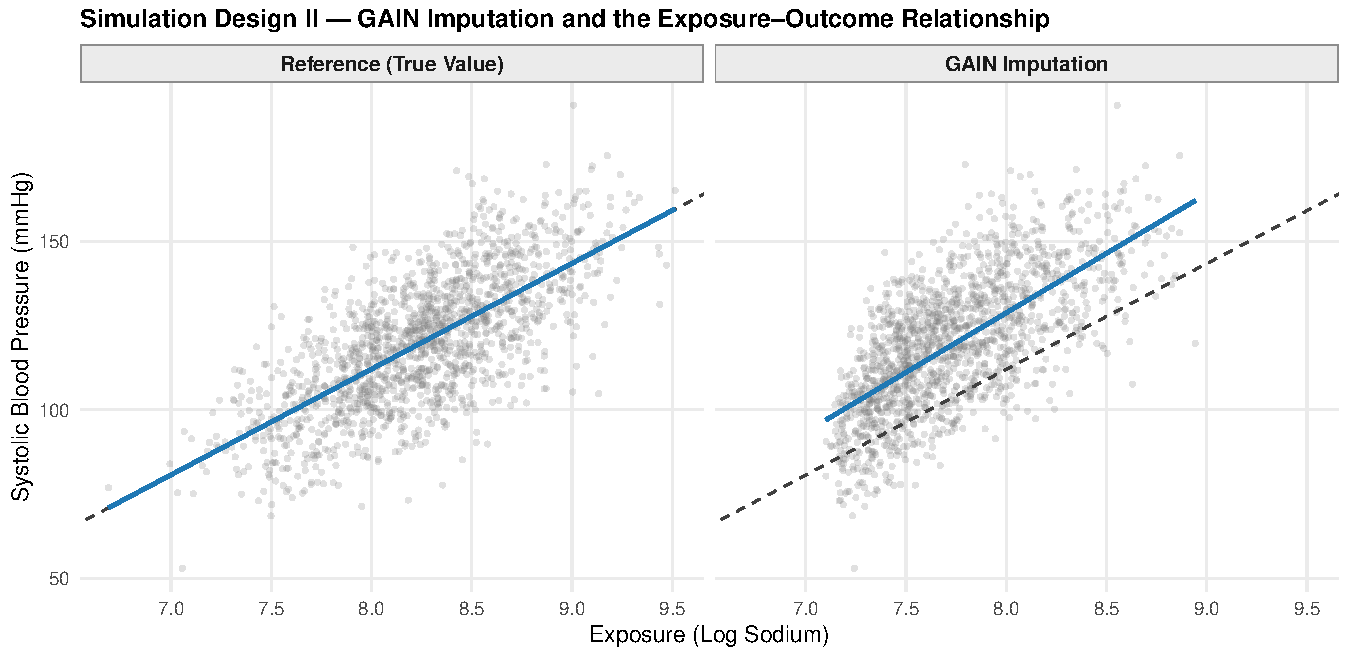
\includegraphics[width=\textwidth]{gain_underdispersion.pdf}
\caption{A trained GAIN model under Simulation Design~II, on a single replicate under simple random sampling. Each panel plots the Gaussian outcome against the exposure for the unvalidated units: the left panel uses the true exposure and the right the GAIN imputation. The dashed line is the true regression fit, repeated in both panels, and the solid line is the fit within each panel. In the right panel the imputed exposure is concentrated near its conditional mean given the outcome, so its spread is compressed and the fitted exposure--outcome line steepens, which is the mechanism by which the distorted imputation biases the downstream coefficient $\hat{\beta}$.}
\label{fig:gain_underdispersion}
\end{figure}


\subsection{Diffusion Models}
\label{sec:diffusion}

Score-based diffusion models \citep{sohl-dickstein2015deep, song2020score} define a forward Markov chain that progressively corrupts a data sample $x_0 \sim q(x)$ into pure noise by adding Gaussian perturbations over a sequence of time steps $t = 1, \ldots, T$. Under the denoising diffusion probabilistic model (DDPM) framework of \citet{ho2020denoising}, the forward transitions are
\begin{equation}
    q(x_t \mid x_{t-1})
    = \mathcal{N}\bigl(x_t;\; \sqrt{1 - \beta_t}\, x_{t-1},\;
      \beta_t I\bigr),
    \label{eq:ddpm_forward}
\end{equation}
where $\{\beta_t\}_{t=1}^T$ is a variance schedule chosen so that $x_T$ is approximately distributed as $\mathcal{N}(0, I)$ for sufficiently large $T$. The generative model parameterises the reverse transitions $p_{\theta}(x_{t-1} \mid x_t)$ and is trained by minimising a reweighted variational bound on the negative log-likelihood, which reduces to a sequence of denoising objectives \citep{ho2020denoising}. The simplified loss function is
\begin{equation}
    L_{\mathrm{DM}}
    = \mathrm{E}_{x_0,\, z \sim \mathcal{N}(0,I),\, t}
    \bigl[\lVert z - z_{\theta}(\sqrt{\bar{\alpha}_t}\, x_0
    + \sqrt{1 - \bar{\alpha}_t}\, z,\; t) \rVert^2\bigr],
    \label{eq:ddpm_loss}
\end{equation}
where $\bar{\alpha}_t = \prod_{s=1}^{t}(1 - \beta_s)$ and $z_{\theta}$ is the noise prediction network.

The connection to score-based modelling \citep{song2019generative, song2020score} provides an alternative perspective: the network learns the score function $\nabla_x \log p_t(x)$, the gradient of the log of $p_t$, where $p_t$ denotes the marginal density after $t$ forward-noising steps, and generation proceeds along the learned score field. Diffusion training does not use the adversarial objective that gives rise to GAN mode-collapse dynamics. A fitted finite network can still approximate the score poorly or miss parts of the target distribution, so the construction does not guarantee complete mode coverage.

For imputation, the reverse diffusion process is conditioned on the observed entries. The conditional score function $\nabla_{x^{\mathrm{mis}}} \log p_t(x^{\mathrm{mis}} \mid x^{\mathrm{obs}})$ guides denoising of the missing entries. \citet{tashiro2021csdi} introduced the Conditional Score-based Diffusion model for Imputation (CSDI), using separate attention modules for temporal and feature dependencies. \citet{zheng2022diffusion} adapted it to tabular data as TabCSDI by removing temporal attention and representing categorical variables through one-hot encoding, analog bits, or feature tokenisation. These representations allow the score model to process mixed data in an encoded continuous space. They do not give TabCSDI a separate multinomial diffusion kernel; that distinction becomes relevant for SIRD in Chapter~\ref{chap:SIRD}.

Several recent extensions have addressed specific limitations of the original diffusion imputation framework. \citet{zhang2025diffputer} combined the EM algorithm with score-based models to handle training on incomplete data, iteratively refining the joint distribution estimate. \citet{liu2024simpdm} introduced self-supervised alignment to reduce sensitivity to the initial noise realisation. \citet{villaizan2025mtabgen} proposed an encoder-decoder transformer with multinomial and Gaussian diffusion kernels to handle heterogeneous feature types in a unified architecture. \citet{zhou2025missddim} adopted non-Markovian deterministic sampling paths to accelerate inference, reducing the number of reverse steps required without sacrificing imputation quality.

Repeated reverse-diffusion runs from different initial noise values provide stochastic draws from the fitted conditional distribution, so one trained model can generate multiple completed datasets. These runs represent variation conditional on the fitted network. They do not vary its fitted parameters and therefore do not constitute the posterior step required for proper multiple imputation. The simulations examine separately whether the resulting coefficient estimates are centred and whether the reported intervals cover under two-phase sampling.

\section{Applicability to Two-Phase Designs}
\label{sec:two_phase_applicability}

The remaining question is which methods have been evaluated for coefficient and interval estimation in settings comparable to a two-phase validation design.

\subsection{Divergent Evaluation Standards in Statistics and Computer Science}
\label{sec:3.5.1}

The statistical and machine-learning literatures have usually evaluated imputation for different purposes. In statistics, imputation is used to support estimation and uncertainty quantification for an analysis parameter $\beta$ \citep{Rubin1987, meng1994multiple}. Relevant evaluations therefore examine the downstream estimator, including its bias and confidence-interval coverage. Section~\ref{sec:eval_metrics} adds oracle diagnostics that separate displacement of the estimate from miscalibration of its standard error. Pointwise prediction error does not answer either question.

In the computer science and machine learning literature, imputation is more commonly treated as a prediction or distribution-recovery task. The most commonly reported evaluation metrics are the root mean squared error (RMSE) between imputed and held-out true values, the mean absolute error (MAE), and, in more recent work, distributional distances such as the Wasserstein distance or maximum mean discrepancy (MMD). Some studies also report predictive performance from a classifier trained on the completed data, using measures such as the area under the receiver operating characteristic curve (AUROC) or the F1 score. These metrics do not, by themselves, establish the bias or interval coverage of a regression estimator fitted to the completed data.

\citet{naf2023imputation} showed across fifteen real datasets that RMSE can favour conditional-mean predictors over methods that draw from a conditional distribution. \citet{naf2025mar} formulated imputation as distributional prediction and advocated proper scoring rules rather than pointwise error alone. These results explain why pointwise and distributional evaluations can rank methods differently. They do not replace direct evaluation of coefficient bias or interval coverage.

\subsection{Evaluation Practices in the Existing Literature}
\label{sec:3.5.2}
To make this divergence concrete, Table~\ref{tab:eval_metrics_lit} catalogues the evaluation metrics reported in the original papers for each imputation method discussed in this chapter. The metrics are classified into three categories: \emph{data-level} metrics that measure pointwise prediction accuracy (RMSE, MAE, classification accuracy); \emph{distribution-level} metrics that assess whether the imputed data recover the joint or marginal distribution of the original data (Wasserstein distance, MMD, energy distance, KL divergence, distributional plots); and \emph{inference-level} metrics that evaluate the properties of a downstream statistical estimator fitted to the imputed data (bias of $\hat{\beta}$, confidence interval coverage, SE ratio, type~I error rate). A method is marked as reporting a given metric only if the original paper includes it in the primary evaluation; downstream prediction accuracy (e.g., AUROC of a classifier) is classified under data-level because it measures predictive performance rather than inferential validity.

\begin{table}[ht]
\centering
\caption{Evaluation metrics reported in the original publications of the imputation methods reviewed in this chapter. A tick (\checkmark) indicates the metric was reported; a dash (--) indicates it was not. Column headers: \textbf{D} = data-level (pointwise prediction); \textbf{Dist} = distribution-level (distributional agreement); \textbf{Inf} = inference-level (downstream statistical inference). For the statistical methods in the first two groups, inference-level evaluation refers to the demonstration of valid inference via Rubin's combining rules, which may take the form of a formal simulation study or an applied analysis reporting bias, variance components, and confidence intervals.}
\label{tab:eval_metrics_lit}
\small
\setlength{\tabcolsep}{4pt}
\begin{tabularx}{\textwidth}{>{\raggedright\arraybackslash}Xccc}
\hline
\textbf{Method} & \textbf{D} & \textbf{Dist} & \textbf{Inf} \\
\hline
\multicolumn{4}{l}{\textit{Joint modelling and FCS}} \\
\texttt{norm/cat/mix} \citep{schafer1997analysis} & -- & -- & \checkmark \\
\texttt{Amelia II} \citep{honaker2011amelia} & -- & -- & \checkmark \\
\texttt{mice} (PMM) \citep{vanBuuren2011} & -- & -- & \checkmark \\
\texttt{jomo} \citep{quartagno2015jomo} & -- & -- & \checkmark \\[2pt]
\multicolumn{4}{l}{\textit{Tree-based and ensemble methods}} \\
\texttt{mice.impute.cart/.rf}$^{\dag}$ \citep{burgette2010multiple, doove2014recursive} & -- & -- & \checkmark \\
\texttt{missForest} \citep{stekhoven2012missforest} & \checkmark & -- & -- \\
\texttt{mixgb} \citep{deng2024multiple} & -- & -- & \checkmark \\[2pt]
\multicolumn{4}{l}{\textit{Autoencoders and VAEs}} \\
MIDA \citep{gondara2018mida} & \checkmark & -- & -- \\
MIDAS \citep{lall2022midas} & \checkmark & -- & \checkmark \\
HI-VAE \citep{nazabal2020handling} & \checkmark & -- & -- \\
VAEAC \citep{ivanov2018variational} & \checkmark & -- & -- \\
MIWAE \citep{mattei2019miwae} & \checkmark & -- & -- \\
MIVAE \citep{ma2023mivae} & \checkmark & -- & -- \\
\texttt{miae} \citep{deng2024thesis} & -- & -- & \checkmark \\[2pt]
\multicolumn{4}{l}{\textit{Generative adversarial networks}} \\
GAIN \citep{yoon2018gain} & \checkmark & -- & -- \\
GAIN variants \citep{wang2021pc, friedjungova2020missing, neves2021sgain} & \checkmark & -- & -- \\
MI-GAN \citep{dai2021multiple} & \checkmark & -- & \checkmark \\[2pt]
\multicolumn{4}{l}{\textit{Diffusion models}} \\
CSDI \citep{tashiro2021csdi} & \checkmark & -- & -- \\
TabCSDI \citep{zheng2022diffusion} & \checkmark & -- & -- \\
DIFFPUTER \citep{zhang2025diffputer} & \checkmark & -- & -- \\
SimPDM \citep{liu2024simpdm} & \checkmark & -- & -- \\
mTabGen \citep{villaizan2025mtabgen} & \checkmark & \checkmark & -- \\
MissDDIM \citep{zhou2025missddim} & \checkmark & -- & -- \\
\hline
\multicolumn{4}{l}{\footnotesize $^{\dag}$\,\texttt{mice.impute.cart} was first proposed by \citet{burgette2010multiple}; the current \texttt{mice}} \\
\multicolumn{4}{l}{\footnotesize implementation and the random forest extension \texttt{mice.impute.rf} are due to} \\
\multicolumn{4}{l}{\footnotesize \citet{doove2014recursive}. Both papers report inference-level metrics.} \\
\end{tabularx}
\end{table}

Table~\ref{tab:eval_metrics_lit} shows that the statistical multiple-imputation methods report coefficient bias, confidence-interval coverage, or both. MIDAS \citep{lall2022midas} and MI-GAN \citep{dai2021multiple} also include an inferential evaluation, and \citet{yoon2018gain} report a limited coefficient analysis for one logistic model. Most other VAE, GAN and diffusion publications in the table report data-level metrics; mTabGen \citep{villaizan2025mtabgen} additionally reports distributional distances. These evaluations do not report confidence-interval coverage or variance calibration.

Evaluation by RMSE alone provides no evidence about coefficient bias or interval calibration. These are separate properties and must be examined directly. A conditional-mean predictor can have low pointwise error while supplying little variation across completed datasets, but the consequences for a particular coefficient and its interval depend on the analysis. For most deep generative methods in Table~\ref{tab:eval_metrics_lit}, those inferential consequences were not tested in the original evaluations.

\subsection{Between-Imputation Variance and the Uncertainty Gap in Deep Generative Models}
\label{sec:uncertainty_gap}

Under Rubin's combining rules \citep{Rubin1987}, the total variance of the multiply imputed estimator decomposes as $\hat{V}_{\mathrm{total}} = \hat{V}_{\mathrm{within}} + (1 + 1/m)\, \hat{V}_{\mathrm{between}}$. The between-imputation term is the variance of the completed-data estimates, not the variance of the missing values themselves. Under proper imputation it reflects the variation in $\hat{\beta}_{\mathrm{com}}$ induced by posterior-predictive draws, including variation in the fitted imputation parameters.

In parametric multiple imputation, this requirement is met through two alternating operations. In the posterior step, the model parameters are drawn from their approximate posterior: $\theta_j^{(t)} \sim P(\theta_j \mid \mathcal{D}_j^{\mathrm{obs}}, \mathcal{D}_{-j}^{(t)})$. In the imputation step, the missing values are drawn conditional on the current parameter realisation: $\mathcal{D}_j^{\mathrm{mis}(t)} \sim P(\mathcal{D}_j^{\mathrm{mis}} \mid \mathcal{D}_j^{\mathrm{obs}}, \mathcal{D}_{-j}^{(t)}, \theta_j^{(t)})$. Because each of the $m$ completed datasets uses a different $\theta_j$ and a different $\mathcal{D}_j^{\mathrm{mis}}$, the between-imputation variance captures both sources of uncertainty simultaneously.

Many deep generative implementations instead fit one network and generate $m$ completed datasets by varying only the stochastic input: a latent draw in a VAE, a noise vector in a GAN, or the reverse-process noise in a diffusion model. In this single-fit procedure, the between-imputation variance reflects variation in the completed-data estimate conditional on one fitted $\hat{\theta}$. It does not include variation across fitted networks.

In the deep learning literature, \citet{gawlikowski2023survey} describe the corresponding distinction as \emph{aleatoric} and \emph{epistemic} uncertainty. This thesis uses the plainer terms \emph{data noise} and \emph{parameter uncertainty}. Repeated training in MIDA and MI-GAN, and Monte Carlo dropout in MIDAS, vary more than the generated input alone. SICG tests Monte Carlo dropout. SIRD uses a proxy-referenced, non-adversarial denoiser that was feasible to fit on a separate bootstrap sample for each completed dataset.

Conditioning on the observed data $\mathcal{D}_{\mathrm{obs}}$, the relevant decomposition is
\begin{equation}
    \mathrm{Var}\bigl(\hat{\beta}_{\mathrm{com}}\mid\mathcal{D}_{\mathrm{obs}}\bigr)
    = \underbrace{\mathrm{Var}_{\theta\mid\mathcal{D}_{\mathrm{obs}}}
      \!\left\{E\bigl(\hat{\beta}_{\mathrm{com}}\mid
      \mathcal{D}_{\mathrm{obs}},\theta\bigr)\right\}}_{\text{parameter uncertainty}}
    + \underbrace{E_{\theta\mid\mathcal{D}_{\mathrm{obs}}}
      \!\left\{\mathrm{Var}\bigl(\hat{\beta}_{\mathrm{com}}\mid
      \mathcal{D}_{\mathrm{obs}},\theta\bigr)\right\}}_{\text{data noise}}.
    \label{eq:var_decomp}
\end{equation}
Proposition~\ref{prop:improper-mi} in Appendix~\ref{app:improper-mi} isolates this omission under Conditions C, M and R: the proper-imputation and single-fit Rubin variance estimators differ by a non-negative parameter-uncertainty component. That result does not by itself prove that every single-fit procedure undercovers. The coverage conclusion in Proposition~\ref{prop:improper-mi-coverage} additionally requires first-order equivalence of the coefficient estimators and a strictly positive limiting variance gap. A smaller validation sample can increase the omitted component by increasing uncertainty in $\theta$, but its size also depends on how the completed-data estimate changes with $\theta$. The simulation results provide the separate evidence about the size and coverage consequence of this gap in the settings studied here.

Reverse-process noise in a diffusion model can represent conditional variation under one fitted score network, and a non-adversarial objective avoids the mode-collapse dynamics of a GAN. Reusing one fitted network still omits variation across training samples and fitted solutions. Model specification and tuning can affect coefficient bias and conditional spread separately from that omission. Chapters~\ref{chap:SICG} and~\ref{chap:SIRD} compare the implemented uncertainty procedures. SICG's Monte Carlo dropout varies masks and generated values around one learned fit, but produces much less between-imputation variance of the fitted coefficients than bootstrap refitting in the reported diagnostic rows. The full SIRD construction improves the coefficient estimate relative to SICG. Its bootstrap fits address the separate interval problem by carrying fitted-model variation into the completed datasets; the study does not attribute the coefficient-estimate improvement to bootstrapping. The Cox interaction remains a separate limitation.

\subsection{Structural Challenges for Two-Phase Imputation}
\label{sec:3.5.4}
Beyond the evaluation gap and the uncertainty gap, the two-phase validation setting imposes structural constraints that differ from the standard missing data problems against which these methods were developed.

Multiple imputation has already been used in validation-subsample analyses, including the dependent-error setting of \citet{giganti2020accounting}, and it can also construct phase-one auxiliaries for raking \citep{han2021combining}. The narrower evidence gap concerns deep generative multiple imputation evaluated by coefficient bias and interval coverage across the two-phase sampling designs studied here. The genotype-imputation application of \citet{luo2024thesis} provides one related setting; this thesis evaluates Gaussian, Binomial and Cox analyses with continuous and categorical phase-two variables.

The first constraint concerns the training objective. A common training device in deep imputation is to create artificial reconstruction tasks by masking entries that are actually observed, and then asking the model to reconstruct them \citep{ma2023mivae, zheng2022diffusion}. This strategy is useful when a large incomplete table contains many observed values from which conditional structure can be learned. In a two-phase validation study, the informative part of the imputation problem is concentrated in the phase-two records. The phase-one variables $(\tilde{X},Y,Z,A)$ are observed for all $N$ units, but the validated variable $X$ is observed only for the validation sample. The analysis-time task is to estimate $P(X\mid \tilde{X},Y,Z,A)$ from the $n$ validated observations and use it for the $N-n$ unvalidated observations. When $n/N$ is small, random masking hides some of this limited validated information during training, while reconstruction losses on the phase-one variables can use capacity on variables that are not imputation targets. The usual self-supervised objective may therefore use the validation sample inefficiently when the missing target block is known in advance.

The second constraint concerns the role of the missingness mechanism. General-purpose deep imputation methods often devote substantial modelling structure to learning, conditioning on, or stabilising across missingness patterns. GAIN uses a hint matrix to guide the discriminator toward the missing entries \citep{yoon2018gain}; VAEAC conditions its networks on the observed-feature set \citep{ivanov2018variational}; MIVAE trains with synthetic corruption to improve performance under varying missingness configurations \citep{ma2023mivae}. These devices are natural when the pattern of missing data is itself irregular or partly unknown. The two-phase problems studied in this thesis are different. The missingness pattern is generated by the validation design and is recorded through the phase-two indicator $R_i$: the validated measurements are observed for selected units and missing for the remaining units. Hence the main difficulty is to use a small validation sample and, when required, its design information to obtain an imputation distribution that gives valid inference for $\hat{\beta}$.

\subsection{Summary}

This chapter reviewed joint modelling, FCS, tree and boosting methods, and three classes of neural generative models. Their multiple-imputation mechanisms differ in two respects that matter for the thesis: the distribution used to draw the missing values and the way fitted-model uncertainty enters the completed datasets.

Table~\ref{tab:eval_metrics_lit} shows that most deep generative methods were evaluated with prediction or distributional metrics rather than confidence-interval coverage. Chapter~\ref{chap:SimDesigns} therefore evaluates coefficient bias and interval coverage directly under the distinct two-phase sampling designs used in the thesis.

\chapter{Simulation Designs and Evaluation Strategy}
\label{chap:SimDesigns}
This chapter defines the simulation framework used to compare the methods in the thesis. It contains three simulation designs and the VCCC case study. Simulation Design~I is an informative-sampling design under a privacy constraint and supports Chapter~\ref{chap:SISL}. Simulation Design~II uses Gaussian and Binomial analysis models, and Simulation Design~III uses a high-dimensional Cox proportional hazards model \citep{therneau2000cox}; these two designs support Chapters~\ref{chap:SICG} and~\ref{chap:SIRD}.

Across these settings, performance is evaluated through inferential criteria rather than purely predictive ones. The reporting block used in the results chapters consists of signed or absolute percentage bias, relative root mean squared estimation error, nominal $95\%$ confidence-interval coverage, and two oracle coverage diagnostics that separate displacement of the coefficient estimate from standard-error calibration. This choice reflects the inferential goals of two-phase studies, where the target is estimation of regression coefficients with calibrated uncertainty, not individual-level prediction accuracy. A full account of these metrics is given in Section~\ref{sec:eval_metrics}.

The notation used in this chapter is defined locally within each simulation design and the case study. In particular, the coefficient vectors $\beta$, $\alpha$, $\theta$ and the variable labels $X_i^{(\cdot)}$, $Z_i^{(\cdot)}$, $Y_i$ are re-defined in each subsection to match the model under discussion, and should not be read as carrying over from one section to another.

\section{Selection of Comparator Methods}
\label{sec:comparators}
The present study evaluates the proposed methods against six comparator approaches. Three of these, \texttt{mice.impute.pmm}, \texttt{mice.impute.rf}, and \texttt{mixgb}, represent widely used tabular multiple-imputation baselines. Two further comparators, GAIN and TabCSDI, are included because they are the early reference methods for GAN-based and diffusion-based imputation respectively, as reviewed in Chapter~\ref{chap:ImpReview}. The sixth comparator, generalised raking, provides a design-based reference for two-phase studies when the relevant phase-one auxiliary information is available.

For fully conditional specification, the study uses two methods from the \texttt{mice} package in \texttt{R} \citep{vanBuuren2011}. The first is \texttt{mice.impute.pmm}, a regression-based donor method that keeps imputed values on the observed support \citep{vanBuuren2018}. The second is \texttt{mice.impute.rf} \citep{doove2014recursive}, which uses random forests to represent non-linear conditional relations and interactions. The two methods keep the chained-equation framework fixed while changing the conditional model.

The third statistical comparator is \texttt{mixgb} \citep{deng2024multiple}, which uses XGBoost \citep{chen2016xgboost} inside the imputation procedure and is among the most competitive general-purpose imputation methods on high-dimensional tabular data; its inclusion reflects that standing. XGBoost learns default splitting directions for missing predictors during tree construction. In the current package, row subsampling contributes stochastic variation across completed datasets and there is no additional bootstrap \citep{deng2026mixgb}. The package default is also \texttt{pmm.type = NULL}, which is the setting used in the thesis.

GAIN and TabCSDI provide neural comparators. GAIN is an early adversarial method designed for missing-data imputation \citep{yoon2018gain}. TabCSDI is an early diffusion method for mixed tabular data \citep{zheng2022diffusion}; diffusion is of interest here because its iterative denoising construction can give better mode coverage than adversarial training in some settings \citep{song2020score}. Their inclusion allows the later chapters to test adversarial and diffusion imputation by coefficient bias and interval coverage, rather than transferring conclusions from prediction and distributional metrics.

Generalised raking provides the design-based comparator \citep{deville1992calibration, lumley2011connections}. It adjusts the phase-two design weights by minimising a smooth distance $g(w_i,d_i)$ from the original weights $d_i$, subject to calibration of weighted phase-two totals to phase-one totals. Raking has been used in two-phase studies \citep{lumley2011connections, breslow2009improved}, including a multinational HIV cohort analysis that combined error-prone and validated data \citep{slone2026analysis}. It is used here as a design-based reference rather than an imputation method. A correctly specified imputation model can be more efficient because it uses a fuller model, while raking retains its design-based role where the required calibration information is available.

\section{Hyperparameter Tuning Protocol}
\label{sec:tuning}
Optimising the selected machine learning comparators requires a tuning protocol whose objective function is aligned with the inferential goals of multiple imputation rather than with standard predictive accuracy criteria. In the traditional machine learning literature, the performance of an imputation method is often evaluated by the root mean squared error (RMSE) or mean squared error (MSE) between the imputed and true masked values \citep{stekhoven2012missforest, yoon2018gain}. For multiple imputation, this criterion is incomplete. Either error can favour methods that approximate the conditional mean $\mathbb{E}[X_{\mathrm{mis}} \mid X_{\mathrm{obs}}]$. Such methods may achieve small pointwise error while understating the conditional spread of $X_{\mathrm{mis}}$, which can reduce the between-imputation component and produce confidence intervals that are too narrow \citep{vanBuuren2018, Rubin1987}. A small masked-value RMSE therefore does not by itself establish that $\hat{\beta}$ has calibrated uncertainty.

\subsection{Evaluation Metric}
As highlighted by \citet{muzellec2020missing}, point-to-point evaluation metrics fail to preserve the underlying geometry and joint distribution of the data. From a statistical perspective, \citet{naf2023imputation} demonstrated that RMSE systematically misranks imputation methods, assigning lower error to conditional-mean predictors than to methods that correctly draw from the conditional distribution. By formalising multiple imputation as intrinsically a distributional prediction task, \citet{naf2025mar} strongly advocate for the use of proper distributional metrics.

For this reason, the present study adopts the energy distance (ED) \citep{szekely2003statistics} as the distributional component of the tuning objective. It is a metric between probability distributions that is estimable directly from samples via pairwise Euclidean distances. In population form, it equals zero if and only if the two distributions are identical, which is a property that pointwise metrics like RMSE are not designed to provide. \citet{naf2025mar} use energy distance rather than optimal transport alternatives, such as the sliced Wasserstein distance \citep{shadbahr2023}, because it is computationally simpler and requires no tuning parameters such as the number of random projections.

For an observed data matrix $X$ of $n$ rows and an imputed data matrix $Y$ of $m$ rows, the empirical energy distance is defined as
\begin{equation}
    \mathrm{ED}(X, Y) \;=\; \frac{2}{nm} \sum_{i=1}^{n}\sum_{j=1}^{m}
    \|X_i - Y_j\|_2
    \;-\; \frac{1}{n^2} \sum_{i=1}^{n}\sum_{j=1}^{n} \|X_i - X_j\|_2
    \;-\; \frac{1}{m^2} \sum_{i=1}^{m}\sum_{j=1}^{m} \|Y_i - Y_j\|_2,
    \label{eq:energy_distance}
\end{equation}
where $\mathrm{ED}(X, Y) \geq 0$ and, in population form, equals zero if and only if $X$ and $Y$ follow the same distribution \citep{szekely2003statistics}. 

The pointwise and distributional losses use different scaling. For MSE, each numeric phase-two target is standardised by its mean and standard deviation in the held-out true rows. For energy distance, the held-out true rows and their imputed versions are combined first, and each numeric column is then standardised in that combined matrix. Categorical variables are expanded by one-hot encoding. The relative scale of a categorical and a continuous variable remains dependent on these choices, so the resulting Euclidean distance is scale-dependent. The study uses it as a common mixed-data discrepancy \citep{naf2025mar}. Because the combined scaling is recomputed for each set of imputations, different trials can be evaluated under different numeric scales. Fixing the scale from the training data would remove this dependence, but it would define a different tuning objective and require the methods to be retuned. All reported configurations use the combined scaling stated here.

The tuning calculation returns three terms. The weighted MSE is scaled by $w_{\mathrm{num}} = n_{\mathrm{num}}/(n_{\mathrm{num}}+n_{\mathrm{cat}})$. The categorical error, written $\mathrm{CatErr}$, is the mean misclassification rate over the categorical phase-two targets and is scaled by $w_{\mathrm{cat}} = n_{\mathrm{cat}}/(n_{\mathrm{num}}+n_{\mathrm{cat}})$. Energy distance is calculated on the full encoded feature space. These terms form two objectives:
\[
\mathcal{L}_{\mathrm{data}}
=w_{\mathrm{num}}\mathrm{MSE}+w_{\mathrm{cat}}\mathrm{CatErr},
\qquad
\mathcal{L}_{\mathrm{dist}}=\mathrm{ED}(X,Y).
\]
The first measures held-out pointwise error and the second measures distributional discrepancy in the chosen representation. Keeping them separate allows the optimisation to retain configurations that trade one discrepancy against the other \citep{naf2023imputation}.

\subsection{Optimisation Procedure}

The R comparators, \texttt{mice.impute.pmm}, \texttt{mice.impute.rf} and \texttt{mixgb}, are tuned with \texttt{mlr3mbo} and ParEGO \citep{bischl2024hyperparameter, knowles2006parego}. GAIN and TabCSDI are tuned with multi-objective Optuna \citep{Akiba2019}. Each comparator is tuned once per setting on one phase-two sample from that setting's reference design: \texttt{InfSamp} for Simulation Design~I and \texttt{SRS} for the remaining settings. Three-fold cross-validation is constructed on the validated rows. Within each fold, the phase-two targets in the validation subset are masked, the method is fitted on the training rows, and both losses are evaluated against the held-out values. The R methods and GAIN use their stated search spaces. TabCSDI uses its full search space in the VCCC case study and the reduced higher-importance set in Simulation Designs~I--III, as described in Appendix~\ref{app:hyperparam}. SICG and SIRD follow the ablation and configuration procedures in their own chapters, and their retained configurations are reused across Simulation Designs~I--III and the VCCC case study.

To reduce the computational cost of evaluating complex neural network architectures, an intermediate pruning strategy is incorporated into the cross-validation loop. After a burn-in period of $\max(10,\, \lfloor 0.25 \times N_{\mathrm{trials}} \rfloor)$ completed trials, any subsequent trial is terminated early if both $\mathcal{L}_{\mathrm{data}}$ and $\mathcal{L}_{\mathrm{dist}}$ simultaneously exceed the 75th percentile of the corresponding loss distributions across all previously completed trials. Under this joint condition, a trial is discarded only when it performs poorly on both objectives at once; trials that achieve a favourable trade-off by sacrificing one objective for the other are preserved.

The completed trials are screened for non-dominance in $(\mathcal{L}_{\mathrm{data}},\mathcal{L}_{\mathrm{dist}})$. Most deployed configurations use the componentwise median of the hyperparameters among the non-dominated trials. The survival random-forest search uses a separate rule because its Pareto set collapsed at a boundary: it takes componentwise medians over the five trials with the lowest min--max-standardised combined loss. In Design~III, \texttt{ntree} and \texttt{mtry} were then reduced manually to control computation; Appendix~\ref{app:config_comparators} records this exception and the retained values. The remaining rules summarise the trial history rather than selecting the Pareto trial with the smallest raw sum of the two losses.

\subsection{Why Inference Metrics Are Not Used as the Tuning Objective}

Coefficient bias and confidence-interval coverage are not used as tuning losses because they are tied to a particular analysis model and require repeated samples to estimate. The completed datasets can support more than one analysis, provided that the imputation model includes the variables, transformations and relationships those analyses require \citep{Rubin1987, meng1994multiple}. Tuning directly to one coefficient would instead select the configuration for that coefficient and model.

Hyperparameters can affect both the coefficient estimate and coverage. They change the fitted conditional distribution and can alter the spread of the completed-data estimates. They cannot, however, add variation across fitted models to a procedure that holds one fitted network fixed. The uncertainty mechanism and the tuning problem are therefore evaluated separately.

The study tunes on $\mathcal{L}_{\mathrm{data}}$ and $\mathcal{L}_{\mathrm{dist}}$ to balance pointwise and distributional discrepancies without choosing one downstream coefficient. Energy distance can detect some forms of under-dispersion in the chosen representation, but it does not establish that the conditional draws are correct or that Rubin's variance is calibrated. Bias and coverage are evaluated later under repeated simulation samples.

\section{Simulation Designs}
\label{sec:simcontext}
Unless otherwise stated, the synthetic simulation settings use $500$ independent population-generation seeds, and the phase-two samples are then drawn using a separate set of independent sampling seeds. The VCCC case study differs from these synthetic settings because the underlying cohort is fixed; there, the repeated experiments come from repeatedly drawing phase-two validation samples from the available validated cohort.

\subsection{Simulation Design I: Informative Sampling under a Privacy Constraint}
\label{sec:infsamp_context}
Simulation Design~I represents a survey-release problem in which the data producer uses confidential stratifying variables and the observed outcome to draw the phase-two validation sample. The selection indicator and design weight are released, while the stratifying variables and joint-stratum label are suppressed. This can occur in public-use survey data when small-area identifiers or sensitive stratifiers are withheld for disclosure control. The analyst can observe unequal selection through $W_i = 1/\pi_i$ and can use the released outcome, but cannot condition directly on the hidden stratifying variables. The design is denoted \texttt{InfSamp} and is analysed in Chapter~\ref{chap:SISL}.

In each synthetic replicate, a population of $N = 10{,}000$ independent individuals is generated. Two suppressed stratifying variables $S_1$ and $S_2$, each taking three equiprobable levels, define nine hidden combinations. The two variables shift both the location and the spread of the validated measurement $X$: the mean for combination $(S_1,S_2)$ is $m_{S_1 S_2} = a_{1,S_1} + a_{2,S_2}$, and the within-combination standard deviation of $X$ increases with this mean. Writing $Z = (Z_1, Z_2, Z_3)$ for three recorded covariates, the validated measurement, the error-prone surrogate and the outcome are generated as
\begin{align}
X_i &= m_{S_{1i} S_{2i}} + \gamma^\top Z_i + \sigma^X_{S_{1i} S_{2i}}\,\varepsilon^X_i, \label{eq:infsamp_X}\\
\tilde{X}_i &= \alpha X_i + \delta^\top Z_i + \tilde{\sigma}\,\tilde{\varepsilon}_i, \label{eq:infsamp_surr}\\
Y_i &= \beta_X X_i + \beta^\top Z_i + \sigma^Y_{S_{1i} S_{2i}}\,\varepsilon^Y_i, \label{eq:infsamp_Y}
\end{align}
with independent standard normal errors and $\beta_X = 0.48$ the estimand of interest in the analysis model $Y \mid X, Z$. The surrogate is non-classical and noisy: it depends on the recorded covariates as well as on $X$ and has residual variance $\tilde{\sigma}^2$. It contains no direct $S_1$ or $S_2$ term, but it remains indirectly associated with the hidden stratifying variables through $X$. The parameter values are listed in Appendix~\ref{app:infsamp}.

The single sampling design of this setting, \texttt{InfSamp}, crosses the nine hidden $(S_1,S_2)$ combinations with three empirical tertiles of the observed outcome $Y$, producing 27 joint sampling strata. The allocation is
\[
n_h \propto N_h s^Y_h,
\]
where $s^Y_h$ is the within-stratum standard deviation of $Y$ in joint stratum $h$, under the total budget $n=500$. The continuous allocation is converted to integer stratum sizes by the exact algorithm of \citet{wright2017exact}. Within each joint stratum the selected units are drawn at random, so the inclusion probability is positive for every individual. For each individual the producer releases $(\tilde{X}_i, Z_i, Y_i)$, the selection indicator $R_i$, and the design weight $W_i = N_h / n_h$; the validated $X_i$ is supplied only for selected individuals. The joint-stratum label and the variables $S_1$ and $S_2$ are not released, while the outcome component of the stratification remains observed.

The design is informative for imputation because phase-two selection depends on the 27 joint strata, while only $Y$ and the resulting design weight are released. The validated records are therefore not a random subset for learning $X\mid \tilde{X},Z,Y$. The released weight $W_i=1/\pi_i$ carries information about the suppressed part of the sampling stratum. Chapter~\ref{chap:SISL} studies whether that weight can be used inside the imputation model to recover the target analysis of $Y$ on $X$ and $Z$.

\subsection{Simulation Design II: Generalised Linear Models}
\label{sec:sim1context}
The population-level dataset adapts the simulation of \citet{baldoni2021use}, which evaluated regression calibration under the three-stage stratified cluster design of the Hispanic Community Health Study \citep{Sorlie2010}. The present study changes its survey design, measurement-error target and outcome models as described below and in Appendix~\ref{app:sim1_data}.

The most substantial structural departure is the removal of the complex survey design entirely. In \citet{baldoni2021use}, a target population of $N = 179{,}268$ individuals is organised into households, block groups, and strata, and phase-one samples of average size approximately $3{,}893$ are drawn via a three-stage stratified sampling scheme. In the present study, we instead simulate a fixed population of $N = 10{,}000$ independent individuals with no clustering or stratification, and the phase-two validation sample of $n = 500$ is drawn directly from this population, yielding a $5\%$ overall sampling fraction. This modification keeps the focus on phase-two missingness and imputation, rather than on additional variation from multistage survey sampling.

The second departure concerns the measurement error structure. The original design involves three tiers: the self-reported naive intake $\tilde{X}_i$ (24-hour recall), the true intake $X_i$, and the biomarker $X^{**}_i$, where $X^{**}_i = X_i + \varepsilon_i$ with $\varepsilon_i \sim \mathcal{N}(0, \sigma^2_\varepsilon)$, and the scientific task is regression calibration from the biomarker. In the present study, the biomarker $X^{**}_i$ is generated but immediately discarded, because there is no direct analogue of a regression calibration task within the generative deep learning framework evaluated in later chapters. The true intake $X_i$ is instead treated directly as the phase-two target variable subject to missingness, and the self-reported intake $\tilde{X}_i$ serves as its phase-one auxiliary. The measurement error model runs in the calibration direction: the true value $X_i$ is generated as a linear function of the surrogate $\tilde{X}_i$ and the fully observed covariates $Z_i$. Taking log-sodium as the primary example, the model is
\begin{equation}
    X_i^{(\mathrm{Na})} \;=\; \gamma_0
    + \gamma_1\, \tilde{X}_i^{(\mathrm{Na})}
    + \gamma_2^{\top} Z_i
    + \delta_i,
    \qquad
    \delta_i \sim \mathcal{N}(0,\, \sigma^2_{\delta}),
    \label{eq:glm_me}
\end{equation}
with analogous models for log-potassium, log-kilocalories, and log-protein. The coefficients $\{\gamma_j\}$ and the error variance $\sigma^2_\delta$ are taken directly from the simulation parameters of \citet{baldoni2021use}, which incorporate the amplification factors applied to the naive intake coefficients and the attenuation of the biomarker error variance described in their Web Appendix~5; no further modification is made in the present study. Full values are given in Appendix~\ref{app:sim1_data}. In this formulation the truth $X_i$ is generated from the surrogate $\tilde{X}_i$. This is the standard calibration regression direction and is the key structural feature that distinguishes this measurement error model from the one used in Simulation Design~III, where the direction is reversed.

The third departure concerns the outcome models. The original coefficients of \citet{baldoni2021use} are retained as the base specification, except that an interaction term $X_i^{(\mathrm{Na})} \cdot Z_i^{(\mathrm{AGE})}$ is added to both the SBP and hypertension models. The interaction supplies a non-additive target for the later imputation comparisons under a $95\%$ phase-two missingness rate.

The first target model is a Gaussian model for systolic blood pressure,
\begin{align}
    Y_i^{(\mathrm{sbp})} \;=\; \beta_0
    &+ \beta_1 Z_i^{(\mathrm{AGE})}
    + \beta_2 Z_i^{(\mathrm{BMI})}
    + \beta_3 X_i^{(\mathrm{Na})}
    + \beta_4 Z_i^{(\mathrm{CHOL})}
    + \beta_5 Z_i^{(\mathrm{BORN})}
    + \beta_6 Z_i^{(\mathrm{SEX})} \nonumber \\
    &+ \beta_7 Z_i^{(\mathrm{PR})}
    + \beta_8 Z_i^{(\mathrm{OTH})}
    + \beta_9 \bigl(X_i^{(\mathrm{Na})} \cdot Z_i^{(\mathrm{AGE})}\bigr)
    + \varepsilon_i,
    \label{eq:app_sbp_model}
\end{align}
with $\varepsilon_i \sim \mathcal{N}(0,\, \sigma^2)$, $\sigma^2 = 145.740$, and true interaction coefficient $\beta_9 = 0.15$. The remaining coefficients are given in Table~\ref{tab:app_outcome_coef}. The second target model is a Binomial model for hypertension status $Y_i^{(\mathrm{htn})} \in \{0,1\}$,
\begin{align}
    \log \frac{\Pr(Y_i^{(\mathrm{htn})} = 1)}{%
              1 - \Pr(Y_i^{(\mathrm{htn})} = 1)}
    \;=\; \alpha_0
    &+ \alpha_1 Z_i^{(\mathrm{AGE})}
    + \alpha_2 Z_i^{(\mathrm{BMI})}
    + \alpha_3 X_i^{(\mathrm{Na})} \nonumber \\
    & + \alpha_4 Z_i^{(\mathrm{CHOL})}
    + \alpha_5 Z_i^{(\mathrm{BORN})}
    + \alpha_6 Z_i^{(\mathrm{SEX})} \nonumber \\
    & + \alpha_7 Z_i^{(\mathrm{PR})}
    + \alpha_8 Z_i^{(\mathrm{OTH})}
    + \alpha_9 \bigl(X_i^{(\mathrm{Na})} \cdot Z_i^{(\mathrm{AGE})}\bigr),
    \label{eq:app_htn_model}
\end{align}
with true interaction coefficient $\alpha_9 = 0.005$.

In total, seven sampling designs are applied to each simulated population to draw the phase-two validation sample: simple random sampling (\texttt{SRS}), residual sampling (\texttt{RS}), weighted residual sampling (\texttt{WRS}), score-function sampling (\texttt{SFS}), outcome-dependent tail sampling (\texttt{ODS-Tail}), outcome-dependent Neyman allocation (\texttt{Neyman-ODS}), and influence-function Neyman allocation (\texttt{Neyman-IF}). Full specifications are given in Appendix~\ref{app:sim1_sampling}. The privacy-constrained informative-sampling setting, \texttt{InfSamp}, is the separate design used in Chapter~\ref{chap:SISL}.

\subsection{Simulation Design III: Complex Survival Data}
\label{sec:sim2context}
Simulation Design~III evaluates the methods in a high-dimensional survival problem that differs from Simulation Design~II. The dataset is constructed for a Cox proportional hazards model of the time from sodium-glucose cotransporter~2 (SGLT2) inhibitor treatment initiation to type~2 diabetes diagnosis. A population of $N = 20{,}000$ independent individuals is generated in each replicate. The construction is synthetic and does not make a clinical claim about SGLT2 inhibitor therapy or type~2 diabetes aetiology. Full technical details are given in Appendix~\ref{app:sim2}.

\subsubsection{Empirical Parameter Derivation}

The simulation parameters for clinical laboratory panels, vital signs, and lifestyle variables are derived from an electronic health record dataset collected at two New Zealand metropolitan hospitals, North Shore Hospital and Waitakere Hospital, covering $530{,}165$ emergency department presentations from July 2016 to June 2021. The dataset contains sociodemographic variables, emergency-department-specific variables, inpatient history, vital signs, laboratory test results from the seven days prior to triage, and dispensing records from the six months prior to triage. Race- and sex-stratified covariance matrices for each laboratory panel are estimated from this EHR dataset using pairwise complete observations. Regression coefficients linking each laboratory outcome to the fully observed demographic predictors are estimated by fitting generalised linear models to the EHR data and retaining only predictors significant at the $p < 0.05$ level. To protect data privacy, small independent Gaussian noise with standard deviation $0.05$ is added to the race-specific regression coefficients before they are used in the simulation. The allele frequencies and linkage disequilibrium (LD) matrices for 15 single-nucleotide polymorphisms (SNPs) are fetched dynamically from the LDlinkR database \citep{Machiela2015}. Together, these parameters give the simulated dataset a complex multivariate dependence structure without reproducing individual patient records.

\subsubsection{Data Structure and Measurement Error Model}
The full variable set spans approximately 120 variables before error-prone versions are added. Both outcome configurations contain phase-one proxies for the SNP genotypes, laboratory measurements and lifestyle indicators. Their validated counterparts form the shared phase-two covariate block. In \texttt{SampleE}, the true survival outcome remains observed for all individuals. In \texttt{SampleOE}, the phase-one data contain error-prone survival variables and their validated counterparts are added to the phase-two target block.

The direction of the error model differs from Simulation Design~II. There, the true dietary intake $X_i$ is generated from the surrogate $\tilde{X}_i$ and the covariates $Z_i$ \citep{baldoni2021use}. In Simulation Design~III, the true clinical variables are generated first from the EHR-derived population model, after which error-prone versions are generated from them. For the continuous variables assigned the common log-scale error model,
\begin{equation}
    \log \tilde{X}_i^{(j)} \;=\; a_0^{(j)}
    + a_1^{(j)} \Bigl(\log X_i^{(j)}
      - \overline{\log X^{(j)}}\Bigr)
    + \mathbf{a}_2^{(j)\top} \tilde{Z}_i^{(j)}
    + e_i^{(j)},
    \qquad
    e_i^{(j)} \sim \mathcal{N}(0,\, \sigma^2_{e,j}),
    \label{eq:surv_me_cont}
\end{equation}
where $a_1^{(j)}$ controls attenuation relative to the truth, $\mathbf{a}_2^{(j)}$ controls the covariate-dependent shift, and $\sigma^2_{e,j}$ is the residual noise \citep{carroll2006seemingly}. These error-model parameters are fixed across simulation replicates. The equation does not describe every continuous proxy. Creatinine receives additive error; error-prone eGFR is derived from error-prone creatinine; error-prone BMI is derived from error-prone weight; and the survival proxies are produced through the altered censoring construction.

For binary and ordinal categorical variables, including smoking status, household income, alcohol use, and exercise level, the measurement error takes the form of a covariate-dependent misclassification model rather than an additive noise model. The probability that the observed surrogate agrees with the true category is
\begin{equation}
    \Pr\!\bigl(\tilde{X}_i^{(j)} = X_i^{(j)}\bigr)
    \;=\; \mathrm{logit}^{-1}\!\bigl(
        q_0 + \mathbf{q}^{\top} \mathbf{c}_i
    \bigr),
    \label{eq:surv_me_cat}
\end{equation}
where $\mathrm{logit}^{-1}(q_0) = p_{j}^{classify}$ is the base classification accuracy and $\mathbf{c}_i$ collects scaled demographic characteristics of individual~$i$. Fixed variable-specific coefficients $\mathbf{q}$ make the misclassification probability depend on the demographic profile. When misclassification occurs, an incorrect category is drawn uniformly from the remaining levels. For the 15 SNP genotypes, a uniform misclassification matrix is applied with diagonal entries $0.990$ and off-diagonal entries $0.005$.

\subsubsection{Outcome Configurations and Sampling Designs}
The present study generates two parallel datasets from each simulated population, referred to as \texttt{SampleE} and \texttt{SampleOE}, which differ in whether the survival outcome variables $(T_I, \Delta, C)$ are themselves included among the phase-two targets. They represent two two-phase data structures that arise in practice.

\texttt{SampleE} corresponds to a common two-phase validation design, in which the outcome $Y$ and the inexpensive covariates $Z$ are fully observed for all phase-one individuals, and only the expensive or error-prone covariates $X$ are subject to validation in the phase-two subsample \citep{tao2017efficient, amorim2021two}. The inferential goal is to recover estimates of $\beta$ despite covariate missingness, while the outcome remains reliably observed for all $N$ individuals. In \texttt{SampleE}, the event time $T_I$, event indicator $\Delta$, and censoring time $C$ are therefore treated as fully observed at phase one, and only the 32 expensive covariate measurements are missing for individuals with $R_i = 0$. Because the survival outcome is fully observed at phase one in this configuration, using $(T_{I,i}, \Delta_i)$ to define the stratification variable for the sampling designs is standard practice in two-phase designs \citep{amorim2021two}.

\texttt{SampleOE} corresponds to a more difficult joint-validation scenario, motivated by the VCCC dependent-error example studied by \citet{giganti2020accounting}. In that setting, error in the recorded treatment start date can propagate into derived covariates, event times and censoring times. In \texttt{SampleOE}, the present study mimics this structure by treating the event time $T_I$, event indicator $\Delta$, and censoring time $C$ as error-prone phase-two targets alongside the expensive covariates, so that for individuals with $R_i = 0$ the outcome variables are also unobserved. The stratification variables for sampling designs are therefore constructed from the surrogate outcome $(\tilde{T}_{I,i}^*, \tilde{\Delta}_i^*)$ rather than the true outcome, since the latter is unavailable at phase one.

The true data-generating Cox model for $T_I$ is specified as
\begin{equation}
\begin{split}
    \lambda(t \mid X_i, Z_i) = \lambda_0(t) \exp\Bigl(
      & \beta_1 X_i^{(\mathrm{HbA1c})}
      + \beta_2 X_i^{(\mathrm{SNP})}
      + \beta_3 Z_i^{(\mathrm{AGE})}
      + \beta_4 X_i^{(\mathrm{eGFR})}  \\
      &+ \beta_5 X_i^{(\mathrm{Insulin})}
      + \beta_6 X_i^{(\mathrm{BMI})}
      + \beta_7 Z_i^{(\mathrm{SEX})}
      + \beta_8 Z_i^{(\mathrm{INS})}  \\
      &+ \beta_9 Z_i^{(\mathrm{RACE})}
      + \beta_{10} X_i^{(\mathrm{SMOKE})}
      + \beta_{11} Z_i^{(\mathrm{AGE})} \times X_i^{(\mathrm{Insulin})}
    \Bigr),
\end{split}
    \label{eq:app_cox_true}
\end{equation}
where all continuous covariates are standardised by location and scale constants chosen to reflect clinically meaningful units (e.g., $(\mathrm{HbA1c} - 50)/5$, $(\mathrm{AGE} - 60)/5$, $(\mathrm{eGFR} - 75)/10$, $(\mathrm{Insulin} - 15)/2$, $(\mathrm{BMI} - 28)/2$). The true hazard ratios are given in Appendix~\ref{app:sim2}. This same model structure is used as the phase-one auxiliary model for the sampling designs described below, with error-prone surrogates $\tilde{X}_i$ replacing the unobserved $X_i$ and, in the \texttt{SampleOE} configuration, the surrogate survival outcome $(\tilde{T}_{I,i}^*, \tilde{\Delta}_i^*)$ replacing the true outcome.

Three sampling designs are applied to each simulated population under each outcome configuration: simple random sampling (\texttt{SRS}), balanced sampling (\texttt{Balanced}), and influence-function Neyman allocation (\texttt{Neyman-IF}). The balanced and Neyman designs share the same joint stratum variable, constructed by crossing the event indicator, survival time interval, HbA1c category, and surrogate smoking status. For the Neyman design, the phase-one auxiliary Cox model is fitted on the surrogate covariates, and the \texttt{dfbeta} residuals for the HbA1c coefficient are extracted to form the individual influence scores used to determine the within-stratum allocation. Full model specifications and sampling design details are given in Appendix~\ref{app:sim2}.

\section{VCCC Case Study}
\label{sec:sim3context}
The Vanderbilt Comprehensive Care Clinic (VCCC) is a large outpatient clinic providing primary and sub-specialty care for patients living with HIV. Its EHR contains demographics, laboratory values, medications and clinical outcomes. The cohort has been used in two-phase sampling and measurement-error research: \citet{amorim2021two} compared validation designs for a Gaussian model, and \citet{giganti2020accounting} developed a multiple-imputation analysis in which treatment-date errors induce dependent errors in covariates and time-to-event outcomes. The EHR-derived records are available with versions obtained through manual chart review, allowing repeated phase-two samples to be compared with a full validated-data benchmark.

The VCCC case study evaluates the methods under Gaussian, Binomial and Cox models. The earlier VCCC analyses focused on one outcome type at a time.

\subsubsection{Data Preprocessing and Variable Derivation}

Following the general processing framework of \citet{amorim2021two}, we partition the available variables into error-free and error-prone categories. Demographic characteristics (sex, race/ethnicity, HIV transmission risk group), mortality status, year of enrolment, and the raw laboratory test results are treated as error-free variables $Z_i$, since these fields are either stable administrative records or objective test values that do not depend on the ART initiation date. The error-prone variables, which are only observed without error in the phase-two validation sample, include the dates of antiretroviral therapy (ART) initiation and cessation, the onset dates of opportunistic infections (OIs), the specific OI diagnosis text, and the ART drug name. These variables constitute the phase-two target vector $X_i$.

The dependent error studied by \citet{giganti2020accounting} arises because laboratory records are mapped to windows anchored at ART initiation. Different reference and EHR-derived ART dates can select different laboratory records even when the laboratory result itself is recorded without error. The retained analysis contains reference and EHR-derived mappings for baseline viral load, so baseline viral load is a phase-two target. Baseline and one-year cluster of differentiation~4 (CD4) counts are mapped using the reference ART date and are treated as fully observed in the analysis models.

We construct the analysis dataset as follows. For each patient, the first validated and unvalidated ART records are identified and linked to the demographic spine. The closest laboratory measurement within a window of $-180$ to $+30$ days relative to the respective ART start date is selected as the baseline value; the one-year CD4 count is mapped analogously with a target date shifted by one year. Patients missing any of the four required laboratory values (validated baseline CD4, validated one-year CD4, validated baseline viral load, unvalidated baseline viral load) after this mapping procedure are excluded, yielding the complete-case analysis cohort.

For the opportunistic infection variables, we retain only the index (first) infection for each patient under both the validated and unvalidated records. A custom text-matching algorithm is applied to the raw diagnosis strings to categorise each OI into clinically meaningful groups. Historical or latent conditions, recorded by phrases such as ``H/O Tuberculosis'' (a documented \emph{history of} tuberculosis) and ``LTBI'' (latent tuberculosis infection), denote past or dormant infection rather than an active opportunistic-infection event. These are neutralised before diagnostic classification so that they do not inflate the opportunistic-infection indicator $D_i$ (Appendix~\ref{app:vccc_preprocessing}). The remaining diagnoses are classified hierarchically. Acquired immunodeficiency syndrome (AIDS)-defining events (ADEs), including \textit{Pneumocystis} pneumonia (PCP), active tuberculosis, \textit{Mycobacterium avium} complex (MAC), toxoplasmosis, cryptococcosis and cytomegalovirus (CMV) end-organ disease, are evaluated before non-ADE infections and non-specific symptoms. A binary indicator $D_i$ records the occurrence of any OI. For the survival analysis, follow-up runs from ART initiation to OI onset or the last clinic visit. Appendix~\ref{app:vccc_preprocessing} gives the text-matching rules and diagnostic categories.

The CD4 counts are square-root transformed and the viral loads are log-transformed prior to analysis, following standard practice in HIV research \citep{amorim2021two}. The final dataset contains both the validated ($X_i$) and unvalidated ($\tilde{X}_i$) versions of all error-prone variables, enabling direct comparison of estimates obtained from the full validated data against those from the error-prone data.

\subsubsection{Target Models}

To evaluate our methods across different outcome types and model structures, we establish three target models for this dataset. Each model is fitted twice: once using the fully validated variables and once using the error-prone unvalidated variables, so that the bias induced by measurement error can be quantified directly.

\paragraph{Model 1: Gaussian model.}
The first target model investigates the association between baseline viral load and immune recovery, measured by the CD4 count at one year after ART initiation. We specify
\begin{equation}
    \mathrm{E}(Y_i \mid X_i, Z_i) \;=\;
    \beta_0
    + \beta_1 X_i^{(\mathrm{VL})}
    + \beta_2 Z_i^{(\mathrm{CD4})}
    + \beta_3 Z_i^{(\mathrm{SEX})}
    + \beta_4 X_i^{(\mathrm{AGE})},
    \label{eq:vccc_gauss}
\end{equation}
where $Y_i = \sqrt{\mathrm{CD4}_{1\mathrm{yr},i}}$ is the square-root transformed CD4 count at one year, $X_i^{(\mathrm{VL})} = \log(\mathrm{VL}_{0,i})$ is the log-transformed validated baseline viral load, $Z_i^{(\mathrm{CD4})} = \sqrt{\mathrm{CD4}_{0,i}}$ is the square-root transformed validated baseline CD4 count, $Z_i^{(\mathrm{SEX})}$ is a binary sex indicator, and $X_i^{(\mathrm{AGE})}$ is the age at validated ART initiation. In this model, the primary error-prone covariate of interest is the baseline viral load $X_i^{(\mathrm{VL})}$; its unvalidated counterpart $\tilde{X}_i^{(\mathrm{VL})}$ is mapped via the error-prone ART start date and therefore inherits the dependent error structure described above. The age at ART initiation $X_i^{(\mathrm{AGE})}$ is also error-prone for the same reason.

\paragraph{Model 2: Binomial model.}
The second model targets the overall risk of experiencing any opportunistic infection. We fit a Binomial model,
\begin{equation}
    \mathrm{logit}\bigl(\Pr(D_i = 1 \mid Z_i, X_i)\bigr) \;=\;
    \alpha_0
    + \alpha_1 Z_i^{(\mathrm{CD4})}
    + \alpha_2 Z_i^{(\mathrm{SEX})}
    + \alpha_3 X_i^{(\mathrm{AGE})}
    + \alpha_4 Z_i^{(\mathrm{YR})},
    \label{eq:vccc_binom}
\end{equation}
where $D_i$ is the binary indicator for any validated OI, and $Z_i^{(\mathrm{YR})}$ is the year of enrolment. In the error-prone version, the outcome $D_i$ itself is replaced by its unvalidated counterpart $\tilde{D}_i$, and the age at ART initiation is replaced by its unvalidated version. This model therefore exhibits simultaneous errors in both a covariate and the binary outcome, a setting that is more challenging than the Gaussian model where the outcome is always correctly observed.

\paragraph{Model 3: Cox proportional hazards.}
The third model is a survival analysis for the time to first OI. We assume the hazard function follows a proportional hazards structure,
\begin{equation}
    \lambda(t \mid Z_i, X_i) \;=\;
    \lambda_0(t) \exp\!\bigl(
        \theta_1 Z_i^{(\mathrm{CD4})}
      + \theta_2 Z_i^{(\mathrm{SEX})}
      + \theta_3 X_i^{(\mathrm{AGE})}
      + \theta_4 Z_i^{(\mathrm{YR})}
    \bigr),
    \label{eq:vccc_cox}
\end{equation}
where $\lambda_0(t)$ is the unspecified baseline hazard and the follow-up time is measured from validated ART initiation to the first validated OI or censoring at the last clinic visit. In the error-prone version, both the event indicator $\tilde{D}_i$ and the follow-up time $\tilde{T}_i$ are derived from the unvalidated ART start date and unvalidated OI onset date, so that the dependent error contaminates the outcome, the covariate, and the risk set simultaneously. This is the most challenging of the three models and directly mirrors the setting studied by \citet{giganti2020accounting}.

For each model, the relative bias of the error-prone estimates is computed as $(\hat{\theta}^{\mathrm{nv}} - \hat{\theta}^{\mathrm{v}}) / \hat{\theta}^{\mathrm{v}}$, where the superscripts denote the non-validated and validated fits respectively. For the Cox model, the relative bias is computed on the hazard ratio scale. These full-data comparisons serve as the benchmark against which the two-phase imputation methods are evaluated in subsequent chapters.


\section{Evaluation Metrics}
\label{sec:eval_metrics}
The metrics below evaluate final performance after tuning and are not tuning objectives. The results chapters use a fixed reporting block: bias, relative root mean squared estimation error, the empirical and mean reported standard errors, nominal coverage, empirical-standard-error oracle coverage, and bias-corrected oracle coverage.

\subsection{Coefficient bias and root mean squared error}

Let $\beta_j$ denote one target coefficient of the substantive analysis model, and let $\hat{\beta}^{(r)}_j$ denote the corresponding estimate in simulation replicate $r = 1,\ldots,M$. The empirical bias is
\begin{equation}
    \mathrm{Bias}_j
    \;=\; \bar{\hat{\beta}}_j - \beta_j
    \;=\; \frac{1}{M} \sum_{r=1}^{M} \hat{\beta}^{(r)}_j - \beta_j,
    \label{eq:eval_bias}
\end{equation}
and, when $\beta_j \neq 0$, the signed percentage bias is $100\,\mathrm{Bias}_j/\beta_j$. Bias records the direction and size of systematic displacement, without recording the dispersion of the estimates around their mean.

Root mean squared estimation error combines these two sources of error. It is defined as
\begin{equation}
    \mathrm{RMSE}_j
    \;=\; \sqrt{\frac{1}{M} \sum_{r=1}^{M}
    \bigl(\hat{\beta}^{(r)}_j - \beta_j\bigr)^2}
    \label{eq:eval_rmse}
\end{equation}
Its exact empirical decomposition is $\mathrm{RMSE}_j^2 = \mathrm{Bias}_j^2 + M^{-1}\sum_{r=1}^{M}(\hat{\beta}^{(r)}_j-\bar{\hat{\beta}}_j)^2$. It is reported as the relative root mean squared estimation error, $\mathrm{RelRMSE}_j = 100\,\mathrm{RMSE}_j/|\beta_j|$, when the relative scale is meaningful. Bias asks whether the estimator is centred correctly, whereas RMSE measures average estimation error from both bias and dispersion. The ablation tables report signed Mean Bias (\%), while the aggregate ranking tables report Mean $|\mathrm{Bias}|$ (\%). In the grouped ranking tables, absolute bias and relative root mean squared estimation error are averaged on the log scale as stated in the table captions. This transformation reduces the influence of an extreme relative error when a true coefficient is close to zero, although the relative metric still requires caution near the null.

\subsection{Confidence-Interval Coverage}

The nominal coverage is the empirical probability that the reported $95\%$ confidence interval contains the target coefficient:
\begin{equation}
    \mathrm{NomCov}_j
    \;=\; \frac{1}{M} \sum_{r=1}^{M}
    \mathbf{1}\!\bigl(
        \hat{\beta}_{j,\mathrm{lo}}^{(r)}
        \leq \beta_j \leq
        \hat{\beta}_{j,\mathrm{up}}^{(r)}
    \bigr),
    \label{eq:eval_coverage}
\end{equation}
where $\hat{\beta}_{j,\mathrm{lo}}^{(r)}$ and $\hat{\beta}_{j,\mathrm{up}}^{(r)}$ are constructed from the analytic standard error reported by the method. For imputation methods this standard error is obtained after combining the completed-data analyses under Rubin's rules \citep{Rubin1987}; for design-based comparators it is obtained from the corresponding survey-weighted variance estimator.

Nominal coverage alone does not identify why an interval misses. The interval can miss because $\hat{\beta}_j$ is displaced, because its reported standard error is too small or too large, or because both occur. Following the simulation-diagnostic practice of \citet{williamson2026assessing} and \citet{morris2019using}, two oracle coverages are therefore reported beside nominal coverage.

The empirical-standard-error oracle, written Orc.\ Cov.\ (Emp), replaces the reported standard error by the Monte Carlo empirical standard error (ESE)
\begin{equation}
    \mathrm{ESE}_j
    \;=\; \Bigl\{ (M-1)^{-1} \sum_{r=1}^{M}
    \bigl(\hat{\beta}^{(r)}_j - \bar{\hat{\beta}}_j\bigr)^2
    \Bigr\}^{1/2}.
    \label{eq:eval_ese}
\end{equation}
Each oracle interval is centred at $\hat{\beta}^{(r)}_j$ with half-width $z_{0.975}\,\mathrm{ESE}_j$. If Orc.\ Cov.\ (Emp) is materially closer to $0.95$ than nominal coverage, replacing the reported standard errors by the empirical spread accounts for part of the coverage difference. This comparison leaves any bias in the centre unchanged. The SE ratio below is needed to determine whether the reported scale is smaller or larger on average.

The bias-corrected oracle, written Orc.\ Cov.\ (BC), instead recentres each estimate by subtracting the empirical bias, $\hat{\beta}^{(r)}_j - \mathrm{Bias}_j$, while keeping the method's reported analytic standard error. If this oracle is close to $0.95$ while the nominal coverage is not, removing average displacement in this hypothetical replacement accounts for much of the coverage difference. When neither oracle coverage approaches the nominal level, both replacements remain inadequate. The diagnostics do not identify the cause of the displacement or distinguish standard-error miscalibration from failure of the Wald approximation.

Two standard-error summaries are reported alongside the coverages. The empirical standard error is $\mathrm{ESE}_j$ of~\eqref{eq:eval_ese}, written Emp.\ SE. It estimates the repeated-sampling standard deviation from the simulation replicates. Among estimators that are centred correctly, a smaller Emp.\ SE indicates greater precision. The mean reported standard error,
\begin{equation}
    \overline{\mathrm{SE}}_j \;=\; M^{-1}\sum_{r=1}^{M} \mathrm{SE}^{(r)}_j,
    \label{eq:eval_meanse}
\end{equation}
written Mean SE, is the average across replicates of the standard error reported by the method. It is obtained from Rubin's rules for the imputation methods and from the survey-weighted variance estimator for the design-based comparators. Emp.\ SE estimates how much the coefficient estimate varies across repeated samples, while Mean SE records the uncertainty reported for each analysed dataset. Their agreement checks the scale of the reported standard error; it does not by itself establish correct coverage when the estimate is biased or the interval approximation is poor. The scale comparison is
\begin{equation}
    \mathrm{SE\ ratio}_j \;=\; \overline{\mathrm{SE}}_j \,/\, \mathrm{ESE}_j ,
    \label{eq:eval_seratio}
\end{equation}
which is read against one. A ratio below one means that the reported standard error is smaller on average than the empirical spread; a ratio above one means that it is larger. The ratio records the direction and size of this scale difference. Its effect on coverage must be interpreted with the estimator's bias, variation in the replicate-specific standard errors, and the adequacy of the interval approximation. Emp.\ SE and Mean SE are read within a coefficient because they retain the coefficient's scale, whereas the SE ratio can be compared across coefficients and methods.

These quantities define the fixed reporting block reused in Chapters~\ref{chap:SISL} to~\ref{chap:SIRD}. The method chapters introduce no additional primary metric; they interpret the same bias, standard errors, relative root mean squared estimation error and coverage diagnostics in the context of each simulation setting.

\subsection{Reading the Complete-Case and Naive References}
\label{sec:cc_reference}

Two reference analyses appear beside the imputation and design-based methods. UNVAL fits the analysis model to the error-prone phase-one variables. CC fits an ordinary unweighted regression to the validated phase-two records and ignores the sampling design. Its behaviour therefore depends on the selection mechanism and the analysis model.

In Simulation Design~II, complete-case bias is low under \texttt{SRS} and the near-proportional \texttt{Neyman-ODS} allocation recorded in Appendix~\ref{app:sim1_sampling}. It is much larger under \texttt{RS}, \texttt{WRS}, \texttt{SFS} and \texttt{ODS-Tail}, which select records from residual, weighted-residual, score-function or outcome tails. The \texttt{Neyman-IF} result lies between these cases, and the privacy-constrained Simulation Design~I also gives material complete-case bias. These are empirical results under the stated designs. They do not imply that complete-case bias must increase monotonically with a general measure of sampling concentration.

\section{Summary}

Six comparator methods are used: \texttt{mice.impute.pmm}, \texttt{mice.impute.rf}, \texttt{mixgb}, GAIN, TabCSDI and generalised raking. The first three represent the main statistical and tree-based imputation baselines, GAIN and TabCSDI represent the early GAN and diffusion imputation references, and raking provides a design-based comparator when its phase-one calibration information is available.

The hyperparameter tuning protocol separates model fitting from downstream inference. Comparator methods are tuned by a bivariate objective combining data-level loss with energy distance \citep{szekely2003statistics, naf2023imputation, naf2025mar}. SICG and SIRD are handled differently: their structural choices are settled by the ablation studies in Chapters~\ref{chap:SICG} and~\ref{chap:SIRD}, and their final configurations are held fixed across the later settings.

The framework contains three simulation designs and the VCCC case study. Simulation Design~I (\texttt{InfSamp}) isolates informative sampling under a privacy constraint for Chapter~\ref{chap:SISL}. Simulation Design~II adapts the dietary validation design of \citet{baldoni2021use} to Gaussian and Binomial outcomes with $95\%$ phase-two missingness. Simulation Design~III is a synthetic high-dimensional survival design with \texttt{SampleE} and \texttt{SampleOE} outcome configurations. The VCCC case study applies the methods to an HIV cohort with validated and EHR-derived records.

Across these settings, performance is judged by inferential criteria rather than pointwise imputation accuracy. The fixed reporting block consists of signed or absolute percentage bias, relative root mean squared estimation error, the empirical and mean reported standard errors, nominal confidence-interval coverage, and two oracle coverage diagnostics. Bias describes centring and RMSE describes repeated-sample error. The two oracle quantities show how coverage changes after replacing either the reported standard error or the average simulation bias. They do not causally assign a coverage failure to one mechanism.

With these benchmarks fixed, each method chapter can ask two separate questions of its method: whether it removes the measurement-error bias, and whether its confidence intervals are correctly calibrated.

\chapter{Sample Imputation via Sample Likelihood}
\label{chap:SISL}
 
\section{Introduction}
\label{sec:SISL_intro}
 
Chapter~\ref{chap:ImpReview} reviewed imputation methods that are in common use for tabular data. This chapter considers a narrower problem. The phase-two sample is drawn by a probability design whose hidden stratifying variables and joint-stratum label are not released. The outcome component of the sampling stratum remains observed. The analyst also observes the error-prone surrogate $\tilde{X}_i$, the recorded covariates, the selection indicator $R_i$, and the design weight $W_i = 1/\pi_i$. The reference measurement $X_i$ is observed only when $R_i = 1$.

The analyst cannot condition on the hidden stratifying variables used for sampling. When complete design variables are available, regression adjustment can be preferable to weight-only adjustment \citep{gelman2007struggles}. When part of that conditioning information is unavailable or cannot be represented in the working model, direct use of the known inclusion probabilities may be needed \citep{robins1997toward}. Design~I has this second structure: the hidden stratifying variables are not merely inconvenient to model, they have been suppressed.

The consequence is an imputation problem. Let $V_i=(\tilde{X}_i,Z_i,A_i,Y_i)$ denote the released phase-one information. Standard multiple imputation fits a model for $X_i\mid V_i$ on the phase-two rows and then uses that fitted model to impute the remaining rows. This is appropriate when $R_i \perp X_i \mid V_i$. Under the informative-sampling design of Section~\ref{sec:infsamp_context}, that conditional independence need not hold, because the suppressed variables are related to $X_i$ and also determine $\pi_i$. The selected rows therefore follow the sample distribution of $X_i\mid V_i,R_i=1$, not necessarily the population distribution of $X_i\mid V_i$ needed for imputation.

This chapter introduces Sample Imputation via Sample Likelihood (SISL). The method uses the released weights inside the fit of the imputation model, rather than treating them only as analysis weights or as another ordinary predictor. Its construction follows the sample-likelihood identity of \citet{pfeffermann1999parametric}, which relates a population density to the corresponding density among selected units through the inclusion probability. The same identity underlies ascertainment-conditional likelihood estimators for two-stage and response-biased samples \citep{breslow1988logistic, scott2011fitting}; the present chapter applies it to the imputation factor instead of directly to the analysis model.
 
The remainder of this chapter is arranged as follows. Section~\ref{sec:SISL_background} sets out the two-phase setting specific to this chapter and introduces the sample-likelihood identity on which the method is built. Section~\ref{sec:SISLmethod} introduces SISL. Section~\ref{sec:SISL_sim} describes the simulation study and the comparators. Section~\ref{sec:SISL_disc} concludes.
 
 
\section{Background}
\label{sec:SISL_background}
 
\subsection{Setting}
\label{sec:SISL_background_setting}
 
We retain the notation of Section~\ref{sec:two_phase}, but specialise it to the privacy-constrained design of Section~\ref{sec:infsamp_context}. The released phase-one information is
\[
V_i = (\tilde{X}_i,Z_i,A_i,Y_i),
\]
where $Y_i$ is included explicitly because it is observed for every unit, enters the imputation models, and is the variable on which the within-stratum Neyman allocation is computed in the informative-sampling simulation. The reference measurement $X_i$ is observed only when $R_i=1$.

The data producer also observes the pair of hidden stratifying variables $C_i=(S_{1i},S_{2i})$, which has nine levels in the simulation of Section~\ref{sec:infsamp_context}. Let $T_i$ denote the empirical tertile of the observed outcome $Y_i$. The sampling stratum is the joint label $H_i=(C_i,T_i)$, so the phase-two sample is allocated across $K=27$ strata and the inclusion probability is constant within joint stratum $h$:
\begin{equation}
\pi_i \;=\; \pi_h \quad \text{for every unit } i \text{ in joint stratum } h,
\label{eq:SISL_piecewise}
\end{equation}
with $\pi_h=n_h/N_h$ determined by the design. The analyst receives $\pi_i$, or equivalently $W_i=1/\pi_i$, for every row in the released data. The outcome and hence $T_i$ remain observed, but the analyst does not receive $C_i$ or the joint-stratum label $H_i$.

Across the levels of $C_i$ the conditional distribution of $X_i$ differs in both mean and variance, so selection through $H_i$ remains associated with $X_i$ after conditioning on the released variables $V_i$. If $C_i$ were released, the imputation model could condition on it directly and estimate $P(X_i\mid V_i,C_i)$. The weights would then mainly describe the sampling design. In the present setting $C_i$ is suppressed, so the model fitted on the selected rows estimates the sample distribution unless the weights are used in some further way. The target for imputation remains the population conditional density
\[
f_p(x\mid V_i;\alpha,\sigma),
\]
because the missing values are needed for the full phase-one cohort, not only for the selected rows.
 
\subsection{Existing approaches and the gap}
\label{sec:SISL_background_gap}
 
A useful way to organise the existing methods is by how they use the released weight. The first option is not to use it. A standard parametric imputation method fits
\begin{equation}
\ell_0(\alpha,\sigma)
\;=\;
\sum_{i:\,R_i = 1} \log f_p(X_i \mid V_i;\alpha,\sigma),
\label{eq:SISL_existing_MI}
\end{equation}
and then draws imputations from the fitted model. This is the baseline to which ordinary chained-equation and automated imputation methods reduce when the weight is excluded. It is justified when the selected rows are representative for $X_i$ after conditioning on $V_i$. It is not generally justified when $R_i$ remains associated with $X_i$ through suppressed design variables.

The second option is to condition on the weight. In a parametric imputation method this means replacing $f_p(X_i\mid V_i;\alpha,\sigma)$ by a model such as $f(X_i\mid V_i,W_i;\alpha,\sigma)$; in automated imputation methods it means allowing $W_i$ to enter the predictor set like any other released variable. This is the model-based route suggested by \citet{gelman2007struggles}: represent the design-relevant information in the model whenever it is available in a usable form. Several survey-imputation papers use related ideas, but their targets are not the same as the one considered here. \citet{marti2011multiple} study multiple imputation for case-cohort data, where the sampling structure is part of the observed design. \citet{seaman2012combining} discuss how multiple imputation and inverse-probability weighting can be combined when missingness and weighting both enter the final analysis. \citet{quartagno2020multiple} use survey weights in a multilevel imputation framework for complex surveys. On the design side, \citet{chen2026generalised} treat a two-phase setting in which the design variables cannot be used as covariates and modify the released weights instead, stabilising them to remove the part of the sampling variation the covariates already explain and combining this with generalised raking to improve the precision of a weighted analysis. Stabilisation and SISL both draw on the relationship between the design weight and the covariates that \citet{pfeffermann1999parametric} formalise, but the former adjusts the weights for a weighted analysis while the latter uses that relationship inside the imputation model. These papers show that weights can enter imputation or analysis in more than one way; they do not derive a sample likelihood for a released-weight design in which the stratifying variables behind $\pi_i$ are suppressed.

The third option is to use the weights in a direct weighted likelihood for the imputation model,
\begin{equation}
\ell_w(\alpha,\sigma)
\;=\;
\sum_{i:\,R_i = 1} W_i\,\log f_p(X_i\mid V_i;\alpha,\sigma).
\label{eq:SISL_weighted_MI}
\end{equation}
This is closer to the survey pseudo-likelihood idea reviewed in Section~\ref{sec:ipw}. It uses the realised weights as case weights and targets a design-weighted population score when the weights are correct. It still does not model the conditional sample density of $X_i$ among selected rows. In particular, it does not account for the fact that, for a fixed $V_i$, the probability of appearing in the validation sample may change across possible values of $X_i$.

The fourth option is to use multiple imputation only as a working model inside a design-based estimator. The raking construction of \citet{han2021combining} is of this type: imputation is used to build an auxiliary variable for calibration, and the final estimator remains a calibrated weighted estimator rather than a completed-data estimator. This is useful as a robust design-based comparator, but it answers a different question. It estimates the analysis parameter $\beta$ for a specified analysis model; it does not produce a reusable imputed dataset whose distribution is intended to represent $X_i\mid V_i$ in the full cohort.

\citet{schildcrout2015biased} is closer in spirit, because the paper studies outcome-dependent subsampling and uses imputation for expensive covariates in a full-cohort analysis. Its imputation distribution is, however, built from a joint model tailored to a longitudinal outcome-dependent design. The present problem is different: the design variables that created the weights are suppressed, and the chapter asks whether the released weights themselves can be used inside the imputation likelihood.

\subsection{Sample-likelihood identity for the imputation factor}
\label{sec:SISL_background_samplelik}

The population imputation density is $f_p(x\mid V_i;\alpha,\sigma)$. The density observed among selected phase-two rows is
\begin{equation}
\begin{aligned}
f_s(x\mid V_i,R_i=1;\alpha,\sigma)
&\;=\;
\frac{\pi^*(x,V_i)\, f_p(x\mid V_i;\alpha,\sigma)}
{D_i(\alpha,\sigma)}, \\
D_i(\alpha,\sigma)
&\;=\;
\int \pi^*(u,V_i)\, f_p(u\mid V_i;\alpha,\sigma)\,\mathrm{d}u,
\end{aligned}
\label{eq:SISL_ps_identity}
\end{equation}
where $\pi^*(x,V_i)=P(R_i=1\mid X_i=x,V_i)$ is the inclusion probability as a function of the reference value and the released phase-one information. This is the sample-distribution identity of \citet{pfeffermann1999parametric}, written for the imputation factor. The outcome $Y_i$ is part of $V_i$ because it is observed at phase one and belongs to the conditioning information used by the imputation model.

Equation~\eqref{eq:SISL_ps_identity} uses the released weight differently from a model that simply adds $W_i$ to the predictor set. Let $H_i$ denote the 27-level joint sampling stratum and let $\pi_h=P(R_i=1\mid H_i=h)$. Since the joint-stratum label is not released, the inclusion probability entering the sample-density identity is not the stratum-specific value $\pi_{H_i}$ itself, but the conditional inclusion function
\[
\pi^*(x,V_i)=P(R_i=1\mid X_i=x,V_i)
=\sum_h \pi_h P(H_i=h\mid X_i=x,V_i).
\]
Thus $\pi^*(x,V_i)$ marginalises over the unreleased joint-stratum label after conditioning on the reference value and the released phase-one variables. The normalising term
\[
D_i(\alpha,\sigma)
=
\int \pi^*(u,V_i) f_p(u\mid V_i;\alpha,\sigma)\,\mathrm{d}u
\]
is the corresponding conditional expectation of $\pi^*(X_i,V_i)$ under the imputation model for $X_i\mid V_i$. The comparison is therefore between two ways of modelling the released weight. The covariate approach conditions directly on the released weight and targets $f_p(X_i\mid V_i,W_i)$. The SISL formulation used here leaves $W_i$ outside the imputation conditioning vector, uses it to estimate the conditional inclusion function $\pi^*(x,V_i)$, and fits $f_p(X_i\mid V_i)$ through the selected-row density in~\eqref{eq:SISL_ps_identity}.

In the two-phase validation literature, related conditional likelihoods have mostly been applied to the analysis-model score. \citet{breslow1988logistic} derived the corresponding likelihood for two-stage case-control logistic regression, where the sampling offset corrects the analysis likelihood. \citet{scott2011fitting} extended the response-biased-sampling likelihood to broader regression families. In both cases the identity produces a direct estimator of the analysis parameter. SISL instead applies the same sample-distribution argument to the imputation model for $X_i\mid V_i$. The resulting completed datasets can then be analysed under the usual multiple-imputation workflow.
 
 
\section{Method}
\label{sec:SISLmethod}
 
\subsection{Sample likelihood for the imputation model}
\label{sec:SISL_method_samplelik}
 
Let $P(X_i \mid V_i;\alpha,\sigma)$ denote a parametric imputation model for the reference measurement, with $V_i = (\tilde{X}_i, Z_i, A_i, Y_i)$ collecting the released phase-one variables together with the outcome, and with $\alpha$ and $\sigma$ a location and a scale parameter. For notational simplicity, this section writes the conditional inclusion function $\pi^*(x,V)$ from Section~\ref{sec:SISL_background_samplelik} as $\pi(x,V)$. A standard imputation fit on the phase-two rows treats those rows as sufficient for learning $f_p(X_i\mid V_i)$. This is appropriate when the validation indicator is conditionally independent of $X_i$ given $V_i$. The privacy-constrained design weakens that condition: the suppressed stratum affects both the realised inclusion probability and the distribution of the reference measurement, while the released variables need not fully recover the stratum. The phase-two data therefore identify a selected-row conditional distribution unless the released information is rich enough to remove the remaining design dependence.

The sample-likelihood identity~\eqref{eq:SISL_ps_identity} requires the conditional inclusion function $\pi(x,V)$ to be available. The strata that generated $\pi_i$ are not released, so $\pi(\cdot)$ is not a known step function over observable boundaries. The released file does contain $W_i = 1/\pi_i$ for every row, and the phase-two rows contain the reference value $X_i$. The sample-distribution argument of \citet{pfeffermann1999parametric} gives
\begin{equation}
E_s(W_i\mid X_i=x,V_i)=\frac{1}{\pi(x,V_i)},
\qquad
\hat{\pi}(x, V) \;=\; \frac{1}{\hat{E}_s\!\left[\,W \mid X = x, V\,\right]}.
\label{eq:SISL_pi_est}
\end{equation}
To see the identity, use
\[
P(H_i=h\mid X_i=x,V_i,R_i=1)
=\frac{\pi_hP(H_i=h\mid X_i=x,V_i)}{\pi^*(x,V_i)}.
\]
It follows that
\[
E_s(W_i\mid X_i=x,V_i)
=\sum_h\frac{1}{\pi_h}
  \frac{\pi_hP(H_i=h\mid X_i=x,V_i)}{\pi^*(x,V_i)}
=\frac{1}{\pi^*(x,V_i)}.
\]
The conditional inclusion function can therefore be estimated without reconstructing the hidden stratum. Its quality depends on the regression for $E_s(W\mid x,V)$ and on phase-two support for the required values of $(x,V)$. Section~\ref{sec:SISL_method_implementation} gives the working specification used in Design~I. In the following derivation, $\pi(\cdot)$ is treated as a smooth function of $(x,V)$.
 
Replacing the population density in~\eqref{eq:SISL_existing_MI} by the conditional density on the selected rows via~\eqref{eq:SISL_ps_identity}, the sample log-likelihood on the phase-two rows is
\begin{equation}
\ell_s(\alpha,\sigma)
\;=\;
\sum_{i:\,R_i = 1}
\left\{
\log P(X_i \mid V_i;\alpha,\sigma)
\;+\; \log \pi(X_i, V_i)
\;-\; \log D_i(\alpha,\sigma)
\right\},
\label{eq:SISL_sample_loglik}
\end{equation}
where
\begin{equation}
D_i(\alpha,\sigma)
\;=\;
E\!\left[\,\pi(X_i, V_i) \mid V_i;\alpha,\sigma\,\right]
\;=\;
\int \pi(x, V_i)\, P(x \mid V_i;\alpha,\sigma)\,\mathrm{d}x
\label{eq:SISL_denominator}
\end{equation}
is the conditional expectation of $\pi(X_i,V_i)$ under the imputation model. Conditional on a fitted or drawn weight-regression parameter $\lambda$, the function $\hat\pi(\cdot,V;\lambda)$ is held fixed while $(\alpha,\sigma)$ are estimated. The numerator value $\log\hat\pi(X_i,V_i;\lambda)$ is then constant with respect to $(\alpha,\sigma)$. The normaliser is not constant: $D_i(\alpha,\sigma;\lambda)$ changes with the distribution assigned to $X_i\mid V_i$. Each draw of $\lambda$ therefore defines a new inclusion surface and requires the sample likelihood to be refitted. When $\pi(\cdot)$ does not vary across the support of $X$, the normaliser equals that common value and the sample log-likelihood reduces to the population log-likelihood~\eqref{eq:SISL_existing_MI}.
 
Under the Gaussian linear specification
\begin{equation}
X_i \mid V_i
\;\sim\;
\mathcal{N}\!\left(\mathbf{w}_i^{\top}\alpha,\;\sigma^2\right),
\qquad
\mathbf{w}_i = (1,\, \tilde{X}_i^{\top},\, Z_i^{\top},\, A_i^{\top},\, Y_i)^{\top},
\label{eq:SISL_gaussian}
\end{equation}
the normaliser is the one-dimensional expectation
\[
D_i(\alpha,\sigma;\lambda)
=E_Z\!\left\{\pi(\mathbf w_i^\top\alpha+\sigma Z,V_i;\lambda)\right\},
\qquad Z\sim\mathcal N(0,1).
\]
The implementation evaluates this expectation numerically at 15 fixed points under the standard normal density. The calculation uses the fitted conditional inclusion surface rather than the original stratum boundaries.
 
For proper multiple imputation in the sense of \citet{Rubin1987}, each imputed dataset requires fresh parameter draws. Let $\lambda$ index the weight regression used to construct $\pi(x,V;\lambda)$, and write $\psi=(\alpha,\log\sigma)$ for the parameters of the population imputation model. For imputation $j$, a draw $\lambda^{(j)}$ is taken from the fitted sampling distribution of the weight regression, the corresponding inclusion surface $\pi^{(j)}(x,V)$ is constructed, and the sample log-likelihood~\eqref{eq:SISL_sample_loglik} is refitted at that surface. A draw $\psi^{(j)}$ is then centred at the resulting sample-likelihood estimate. Section~\ref{sec:SISL_method_implementation} defines the three covariance rules used for these two stages.
 
\begin{proposition}
\label{prop:SISL_consistency}
Let $(\alpha_0,\sigma_0)$ denote the population-level parameters of the imputation model~\eqref{eq:SISL_gaussian}, and let $(\hat{\alpha},\hat{\sigma})$ denote the maximiser of the sample log-likelihood~\eqref{eq:SISL_sample_loglik}. Suppose that
\begin{enumerate}[label=(\roman*)]
\item the imputation model~\eqref{eq:SISL_gaussian} is correctly specified; and
\item the inclusion model $\pi(x, V)$ is correctly specified, in the sense that the weight regression~\eqref{eq:SISL_pi_est} is consistent for $E_s[W \mid x, V]$.
\end{enumerate}
Then, under standard regularity conditions \citep{newey1994large}, the estimator $(\hat{\alpha},\hat{\sigma})$ is consistent for $(\alpha_0,\sigma_0)$ as $n \to \infty$.
\end{proposition}
 
\begin{proof}[Proof sketch]
Under conditions (i) and (ii), the sample log-likelihood~\eqref{eq:SISL_sample_loglik} is the correctly specified log-likelihood for the conditional density of $X_i$ on the selected rows given by~\eqref{eq:SISL_ps_identity}, with $\pi(\cdot)$ of~\eqref{eq:SISL_pi_est} in the role of the inclusion probability. The correction terms $\log \pi(X_i, V_i)$ and $\log D_i(\alpha,\sigma)$ are then, respectively, free of the imputation-model parameters and a known functional of $(\alpha,\sigma)$, so the expected sample log-likelihood $E[\ell_s(\alpha,\sigma)]$ is a function of $(\alpha,\sigma)$ alone. Under standard identifiability and regularity conditions, it is uniquely maximised at $(\alpha_0,\sigma_0)$, and the conclusion follows from the uniform convergence argument of \citet{newey1994large}, Theorem~2.1. The structure of the proof is the same as the parametric case in Section~3.1 of \citet{pfeffermann1999parametric}, with the analysis-model density replaced by the imputation-model density throughout. Condition (ii) is essential and is not automatic: because $\pi(\cdot)$ is estimated rather than known, a misspecified weight regression carries directly into a bias in $(\hat{\alpha},\hat{\sigma})$, a point returned to in Section~\ref{sec:SISL_method_implementation}.
\end{proof}

The privacy constraint prevents direct reconstruction of the original stratum rule, but it does not prevent identification of the conditional inclusion function. Equation~\eqref{eq:SISL_pi_est} identifies $\pi(x,V)$ through the selected-sample conditional mean of the released weight. Consistency still requires the fitted regression for that conditional mean to be adequate over the relevant support. The spline model used below is a working model for Design~I. Any remaining coefficient bias can reflect its approximation error, the Gaussian imputation model, or finite-sample estimation; the simulation does not separate these sources.
 
 
\subsection{Imputation draws for unsampled units}
\label{sec:SISL_method_imputation}
 
The fit of Section~\ref{sec:SISL_method_samplelik} targets the population parameters $(\alpha,\sigma)$ using the selected rows. Imputation is required for units with $R_i=0$. Given $V_i$, their distribution differs from the population model whenever $1-\pi(x,V_i)$ varies with $x$. The imputation distribution must therefore condition on non-selection.
 
By Bayes' rule, and using $P(R_i = 0 \mid X_i = x, V_i) = 1 - \pi(x, V_i)$,
\begin{equation}
f_0(x \mid V_i, R_i = 0;\alpha,\sigma)
\;=\;
\frac{\bigl(1 - \pi(x, V_i)\bigr)\, f_p(x \mid V_i;\alpha,\sigma)}
{1 - D_i(\alpha,\sigma)},
\label{eq:SISL_fR0}
\end{equation}
where $1 - D_i(\alpha,\sigma)$ is the marginal probability of non-selection under the imputation model, with $D_i$ as in~\eqref{eq:SISL_denominator}. The non-selection density is the population imputation density tilted by the factor $1 - \pi(x, V_i)$, which up-weights the regions of low inclusion probability that the phase-two sample under-represents.
 
Because the estimated $\hat{\pi}(\cdot)$ is a smooth function of $(x, V)$ rather than a step function with known boundaries, the density~\eqref{eq:SISL_fR0} is not of a standard parametric form, and a rejection scheme with a simple envelope is no longer convenient. The density is univariate and bounded, so it is sampled by inversion on a fine grid. For each unsampled unit, the population density $f_p(x \mid V_i;\hat{\alpha}^{\star},\hat{\sigma}^{\star})$ and the factor $1 - \hat{\pi}(x, V_i)$ are evaluated on a common grid spanning the support used by the imputation model. Their product is normalised to approximate~\eqref{eq:SISL_fR0}, and a uniform draw is mapped through the resulting cumulative distribution by linear interpolation. Each imputed value $X_{i,\mathrm{mis}}^{(j)}$ uses a fresh parameter draw rather than a single fixed estimate, so the fitted-model uncertainty represented by the chosen covariance estimator enters the imputations.
 
The complete procedure is summarised in Algorithm~\ref{alg:sisl}.
 
\begin{algorithm}[t]
\caption{Sample imputation via sample likelihood (SISL)}
\label{alg:sisl}
\begin{algorithmic}[1]
    \Require reference $X_i$ for $\{i : R_i = 1\}$;
             released weights $W_i = 1/\pi_i$ for $i = 1,\ldots,N$;
             phase-one variables $V_i$;
             $m$: number of imputations
    \State Fit the weight regression on $\{i:R_i=1\}$ to obtain $\hat\lambda$, with
           $\hat\pi(x,V;\lambda)=1/\hat E_s[W\mid x,V;\lambda]$
    \State Fit the sample likelihood at $\hat\lambda$ and estimate the covariance pair
           $(\hat V_\lambda,\hat V_\psi)$ by the selected model-based, sandwich,
           or bootstrap rule
    \For{$j = 1,\ldots,m$}
        \State Draw $\lambda^{(j)}\sim\mathcal N(\hat\lambda,\hat V_\lambda)$ and
               set $\pi^{(j)}(x,V)=\hat\pi(x,V;\lambda^{(j)})$
        \State Maximise the sample log-likelihood on $\{i:R_i=1\}$,
               \[
               \ell_s(\alpha,\sigma;\pi^{(j)})
               =\sum_{R_i=1}\left\{
               \log f_p(X_i\mid V_i;\alpha,\sigma)
               -\log D_i(\alpha,\sigma;\pi^{(j)})
               \right\},
               \]
               where $D_i$ is evaluated as the numerical expectation in
               \eqref{eq:SISL_denominator}, to obtain
               $\hat\psi^{(j)}=(\hat\alpha^{(j)},\widehat{\log\sigma}^{(j)})$
        \State Draw $\psi^{(j)}\sim\mathcal N(\hat\psi^{(j)},\hat V_\psi)$
               \hfill\textit{(parameter-draw step)}
        \For{each $i$ with $R_i = 0$}
            \State Draw $X_{i,\mathrm{mis}}^{(j)}$ from the non-selection density~\eqref{eq:SISL_fR0}
                   by grid inversion, using $\psi^{(j)}$ and $\pi^{(j)}(\cdot)$
                   \hfill\textit{(imputation step)}
        \EndFor
    \EndFor
    \State \Return $\{X_{i,\mathrm{mis}}^{(j)} : R_i = 0,\; j = 1,\ldots,m\}$
\end{algorithmic}
\end{algorithm}
 
 
\subsection{Design I implementation and covariance estimators}
\label{sec:SISL_method_implementation}
 
The Design~I simulation uses a standalone R routine. It receives the reference measurement on the phase-two rows, the released phase-one variables and the released weight. The hidden stratifying variables and the joint-stratum label are not inputs. The conditional inclusion function is estimated from the selected rows through the working regression
\begin{equation}
\begin{aligned}
L_i
&= \log(W_i-1) \\
&= \gamma_0
 + \mathbf b_{X,6}(X_i)^\top\gamma_X
 + \mathbf b_{Y,5}(Y_i)^\top\gamma_Y
 + \{\mathbf b_{X,4}(X_i)\otimes\mathbf b_{Y,3}(Y_i)\}^\top\gamma_{XY}
 + Q_i^\top\gamma_Q + e_i,
\end{aligned}
\label{eq:SISL_weight_model}
\end{equation}
where $\mathbf b_{X,d}$ is a $d$-term B-spline basis, $\mathbf b_{Y,d}$ is a $d$-term natural-spline basis, and $Q_i=(\tilde X_i,Z_{1i},Z_{2i},Z_{3i})^\top$. The coefficients are fitted by least squares on the phase-two rows. With fitted mean $\hat\eta(x,V)$ and residual variance $\hat\tau^2$, the working shifted log-normal calculation gives
\begin{equation}
\widehat E_s(W\mid x,V)
=1+\exp\{\hat\eta(x,V)+\hat\tau^2/2\},
\qquad
\hat\pi(x,V)
=\left[1+\exp\{\hat\eta(x,V)+\hat\tau^2/2\}\right]^{-1}.
\label{eq:SISL_weight_surface}
\end{equation}
This specification was chosen for Design~I. The interaction allows the weight surface to change jointly with the reference measurement and the observed outcome. It is not a general specification for other sampling designs.

The residual variance $\hat\tau^2$ is held at its full-phase-two estimate when the weight-regression coefficients are drawn. The variance comparison below does not add a separate draw for this shift term.

The spline basis for $X$ is evaluated at the nearest boundary when the likelihood or imputation grid extends outside the range of the phase-two reference values. This avoids extrapolating the fitted weight regression beyond its observed support. For each likelihood evaluation, $D_i$ is calculated from the 15-point numerical expectation described after~\eqref{eq:SISL_gaussian}. The sample likelihood is maximised by the Broyden--Fletcher--Goldfarb--Shanno algorithm. Missing reference values are then drawn by the grid inversion in Section~\ref{sec:SISL_method_imputation}.

The three SISL variants use different covariance estimators at both fitted stages. Let $P$ be the design matrix in~\eqref{eq:SISL_weight_model}, let $H$ be the observed Hessian of the negative sample log-likelihood, and let $J$ be the outer product of its rowwise scores. SISL-M uses the classical least-squares covariance $\hat\tau^2(P^\top P)^{-1}$ for the weight regression and $H^{-1}$ for the main imputation-model parameters. SISL-S uses an HC0 covariance for the weight regression and $H^{-1}JH^{-1}$ for the main parameters. SISL-B uses the empirical covariance of 100 bootstrap refits at each stage. The weight-model spline bases are rebuilt in each weight-model resample. The main-model bootstrap refits use the inclusion surface from the full phase-two fit. The two bootstrap covariances are estimated separately.

All three variants use the same draw sequence. For each imputation, a weight-coefficient draw defines a new inclusion surface. The sample likelihood is refitted on all phase-two rows at that surface, and the main imputation-model parameters are drawn around the refitted values. The two covariance matrices are calculated once from the full phase-two fits and are reused across the $m=20$ imputations.

The model-based covariance would be exact only if the fitted sample likelihood were the true selected-row density. It is not. The inclusion function is a step surface over the suppressed strata, and across those strata $X_i$ shifts in both mean and variance, so the fit of Section~\ref{sec:SISL_method_implementation} recovers it only as a smooth function of the released variables. The sample likelihood built on that smooth fit is a working approximation, and the model-based covariances taken at the two fitted stages understate the repeated-sampling spread of the estimates. The sandwich and the bootstrap do not assume the fit is exact. The sandwich estimates the spread from the per-observation scores, and the bootstrap resamples the phase-two rows and refits both stages \citep{huber1967behavior,white1982maximum}.

\begin{table}[!htbp]\centering
\caption{Variance calibration of the three SISL constructions on the exposure coefficient $\beta_X$ of the informative-sampling design, over $500$ replicates. The empirical standard error (Emp.\ SE) is the standard deviation of the coefficient estimates, and Mean SE is the mean reported standard error. Their ratio summarises calibration, and nominal coverage (Nom.\ Cov.) is assessed against $0.95$. The empirical-standard-error oracle coverage, Orc.\ Cov.\ (Emp), replaces the reported standard error with the empirical standard error. All variants draw the weight-regression parameters; SISL-M, SISL-S and SISL-B use model-based, sandwich and bootstrap covariance, respectively, at both fitted stages.}
\label{tab:sisl_variance}
\small
\begin{tabular}{lrrrrr}
\toprule
Variance source & \multicolumn{1}{c}{Emp.\ SE} & \multicolumn{1}{c}{Mean SE} & \multicolumn{1}{c}{SE ratio} & \multicolumn{1}{c}{Nom.\ Cov.} & \multicolumn{1}{c}{Orc.\ Cov.\ (Emp)} \\
\midrule
SISL-M (model-based) & 0.040 & 0.029 & 0.72 & 0.83 & 0.94 \\
SISL-S (sandwich) & 0.039 & 0.037 & 0.95 & 0.94 & 0.95 \\
SISL-B (bootstrap) & 0.039 & 0.043 & 1.10 & 0.96 & 0.95 \\
\bottomrule
\end{tabular}
\end{table}

SISL-M reports a mean standard error of $0.029$ against an empirical standard error of $0.040$, giving an SE ratio of $0.72$. Its intervals cover in $0.83$ of the replicates. Replacing the reported standard error by the empirical standard error raises the oracle coverage to $0.94$, so the scale difference accounts for most of the observed undercoverage. SISL-S has an SE ratio of $0.95$ and coverage of $0.94$. SISL-B has an SE ratio of $1.10$ and coverage of $0.96$, indicating slight overestimation of the repeated-sample spread. These results support sandwich or bootstrap covariance for the two-stage SISL procedure in Design~I. The model-based covariance is too small because it treats the smooth inclusion fit as exact, when that fit only approximates the step selection over the suppressed strata across which $X_i$ varies in mean and variance.

In the simulation study of Section~\ref{sec:SISL_sim}, SISL imputes the single reference measurement $X_i$; the remaining released variables are observed for every unit and enter the imputation and inclusion models as predictors.
 
 
\section{Simulation study}
\label{sec:SISL_sim}

\subsection{Design}
\label{sec:SISL_sim_setup}

The method is assessed on the informative-sampling design under a privacy constraint introduced in Section~\ref{sec:infsamp_context}, whose data generation and sampling are set out in full in Appendix~\ref{app:infsamp}. Each simulated population contains $N = 10{,}000$ units. The phase-two validation sample of $n = 500$ is allocated across 27 joint strata formed by the nine hidden $(S_1,S_2)$ combinations and three observed-$Y$ tertiles. The released data carry the weight $W_i = 1/\pi_i$, the surrogate $\tilde{X}_i$, the covariates $Z_i$ and the outcome $Y_i$, but not the hidden stratifying variables or joint-stratum label. The reference measurement $X_i$ is observed on the phase-two rows and is the target of imputation. Its coefficient $\beta_X$ is estimated in the Gaussian analysis model $Y_i = \beta_X X_i + Z_i^{\top}\beta_Z + \varepsilon_i$.

The comparison is organised around the role of the released weight. The first estimator ignores it and imputes $X$ from the released variables; this is the naive multiple imputation that Section~\ref{sec:SISL_background_gap} identifies as vulnerable when the selected rows do not represent $X_i\mid V_i$. The second enters the factor-coded weight as an additional covariate, testing whether it can serve as a modelling surrogate for the hidden stratifying variables. Weighted-likelihood multiple imputation (WLMI) instead uses $W_i=1/\pi_i$ as a case weight in the imputation-model likelihood and propagates parameter uncertainty by a Bayesian bootstrap. SISL uses the released weights to estimate the conditional inclusion function in Section~\ref{sec:SISLmethod}. These four approaches compare ignoring the weight, conditioning on it, using it directly in the likelihood, and using it to estimate the sample-likelihood correction.

Alongside these four, the imputation methods that serve as comparators throughout the thesis, described in Section~\ref{sec:comparators}, are applied to the same design. This places methods that use the released weight in the likelihood or analysis beside methods that do not. Performance is summarised by the benchmark block of Section~\ref{sec:eval_metrics}.







\subsection{Results}
\label{sec:SISL_sim_results}

Table~\ref{tab:sisl_rank} reports the benchmark block for the exposure coefficient $\beta_X$ over the $500$ replicates. The full per-method metrics, broken down by coefficient group, are collected in Table~\ref{tab:appc_sisl}, and the per-replicate percentage-bias distributions for the exposure and for the Phase-One covariates are shown in Figures~\ref{fig:sisl_pctbias} and~\ref{fig:sisl_phase1cov}, all in Appendix~\ref{app:suppC_sisl}.

\begin{table}[!htbp]\centering
\definecolor{rankone}{RGB}{33,113,181}\definecolor{ranktwo}{RGB}{107,174,214}\definecolor{rankthree}{RGB}{198,219,239}
\caption{Method performance on the exposure coefficient $\beta_X$ of the informative-sampling design, over 500 replicates. Mean $|$Bias$|$ and relative RMSE of the coefficient estimate are in per cent; the empirical standard error (Emp.\ SE) and mean reported standard error (Mean SE) are on the coefficient scale, and their ratio summarises variance calibration. The three coverages are assessed against $0.95$. Mean $|$Bias$|$ and relative RMSE are ranked ascending, and the SE ratio and coverages by proximity to their targets. The three best distinct ranks in each shaded column, including the complete-case (CC) and naive-proxy (UNVAL) references, are shown by colour; displayed ties receive the same shade. SICG and SIRD are introduced in Chapters~\ref{chap:SICG} and~\ref{chap:SIRD}; SISL-S and SISL-B use sandwich and bootstrap covariance. TabCSDI is computed over 100 of the 500 replicates.}
\label{tab:sisl_rank}
\scriptsize
\setlength{\tabcolsep}{4pt}
\adjustbox{max width=\linewidth}{%
\begin{tabular}{lrrrrrrrr}
\toprule
Method & \multicolumn{1}{c}{Mean $|$Bias$|$ (\%)} & \multicolumn{1}{c}{Rel.\ RMSE (\%)} & \multicolumn{1}{c}{Emp.\ SE} & \multicolumn{1}{c}{Mean SE} & \multicolumn{1}{c}{SE ratio} & \multicolumn{1}{c}{Nom.\ Cov.} & \multicolumn{1}{c}{Orc.\ Cov.\ (Emp)} & \multicolumn{1}{c}{Orc.\ Cov.\ (BC)} \\
\midrule
CC & 14.7 & 18.0 & 0.050 & 0.047 & 0.94 & 0.65 & 0.69 & \cellcolor{rankthree}0.93 \\
UNVAL & 77.4 & 77.5 & 0.005 & 0.005 & \cellcolor{rankone}1.00 & 0.00 & 0.00 & \cellcolor{ranktwo}0.94 \\
NAIVE & 13.4 & 15.1 & 0.034 & 0.031 & 0.91 & 0.49 & 0.53 & 0.92 \\
NAIVE+W & 14.2 & 15.8 & 0.033 & 0.030 & 0.91 & 0.45 & 0.47 & 0.92 \\
WLMI & \cellcolor{ranktwo}0.9 & \cellcolor{rankone}7.6 & 0.036 & 0.038 & 1.06 & \cellcolor{rankone}0.95 & \cellcolor{rankone}0.95 & \cellcolor{ranktwo}0.94 \\
RAKING & \cellcolor{rankone}0.3 & \cellcolor{rankthree}8.5 & 0.041 & 0.040 & \cellcolor{ranktwo}0.98 & \cellcolor{rankone}0.95 & \cellcolor{rankone}0.95 & \cellcolor{rankone}0.95 \\
MICE-PMM & 7.4 & 9.9 & 0.031 & 0.028 & 0.90 & \cellcolor{rankthree}0.76 & \cellcolor{rankthree}0.79 & 0.90 \\
MICE-RF & 12.0 & 13.9 & 0.034 & 0.014 & 0.41 & 0.18 & 0.61 & 0.58 \\
MIXGB & 130.5 & 131.4 & 0.076 & 0.041 & 0.54 & 0.00 & 0.00 & 0.71 \\
GAIN & 10.2 & 67.3 & 0.320 & 0.011 & 0.03 & 0.03 & \cellcolor{rankone}0.95 & 0.05 \\
TabCSDI & 18.9 & 24.4 & 0.075 & 0.015 & 0.20 & 0.12 & 0.72 & 0.24 \\
\textbf{SICG} & 6.6 & 12.3 & 0.050 & 0.013 & 0.26 & 0.37 & \cellcolor{ranktwo}0.90 & 0.45 \\
\textbf{SIRD} & 19.8 & 21.1 & 0.034 & 0.051 & 1.50 & 0.60 & 0.21 & 0.98 \\
\textbf{SISL-S} & 3.0 & 8.7 & 0.039 & 0.037 & \cellcolor{rankthree}0.95 & \cellcolor{ranktwo}0.94 & \cellcolor{rankone}0.95 & \cellcolor{ranktwo}0.94 \\
\textbf{SISL-B} & \cellcolor{rankthree}2.2 & \cellcolor{ranktwo}8.4 & 0.039 & 0.043 & 1.10 & \cellcolor{ranktwo}0.96 & \cellcolor{rankone}0.95 & \cellcolor{ranktwo}0.96 \\
\bottomrule
\end{tabular}}
\end{table}

The methods that ignore the released weight retain substantial bias. NAIVE has $13.4\%$ bias and $15.1\%$ relative RMSE. This is consistent with fitting the conditional distribution among the selected rows when selection remains informative given the released predictors. Entering the factor-coded weight as a main effect does not change the result: NAIVE+W has $14.2\%$ bias and $15.8\%$ relative RMSE. This comparison assesses the tested factor-covariate specification. It does not rule out a richer outcome model containing interactions between the weight and the other predictors.

WLMI and raking use the realised inverse inclusion probabilities directly. WLMI has $0.9\%$ bias and $7.6\%$ relative RMSE, while raking has $0.3\%$ bias and $8.5\%$ relative RMSE. SISL-S and SISL-B also remove most of the bias left by NAIVE. Their biases are $3.0\%$ and $2.2\%$, and their relative RMSEs are $8.7\%$ and $8.4\%$. These four procedures have nominal coverage between $0.94$ and $0.96$. In this design, the fitted conditional inclusion surface reduces bias and gives near-nominal coverage, but it does not improve on methods that use the realised weights directly.

The comparison of SISL-S and SISL-B is mainly a variance comparison. Their empirical standard errors are both $0.039$. The sandwich version reports a mean standard error of $0.037$, and the bootstrap version reports $0.043$. Their corresponding coverages of $0.94$ and $0.96$ agree with the calibration results in Table~\ref{tab:sisl_variance}. The small difference between their coefficient biases is not evidence that one covariance rule improves centring; the simulation was not designed to separate that difference from Monte Carlo and imputation variation.

The general-purpose methods show different failures. MICE-PMM reduces the bias to $7.4\%$, but its SE ratio of $0.90$ and coverage of $0.76$ remain below the SISL, WLMI and raking results. MICE-RF and TabCSDI report much smaller standard errors than the repeated-sample spread, with SE ratios of $0.41$ and $0.20$. GAIN has a mean absolute bias of $10.2\%$, but its relative RMSE is $67.3\%$ and its empirical standard error is $0.320$. Its mean reported standard error is only $0.011$. MIXGB has $130.5\%$ bias in this setting. These results show that a moderate average bias alone does not establish stable coefficient estimation or calibrated intervals.

SICG and SIRD are included in the table for comparison with later chapters. Their construction and uncertainty procedures have not yet been introduced, so their Design~I results are not interpreted here. More generally, the oracle columns are hypothetical replacements of the reported standard error or the average bias. They help describe an interval failure but do not identify its cause.

\section{Discussion}
\label{sec:SISL_disc}

Design~I separates two forms of available sampling information. The analyst observes each realised weight and the outcome component of the sampling stratum, while the other stratifying variables are withheld. Equation~\eqref{eq:SISL_pi_est} shows that this suppression does not prevent identification of the conditional inclusion function. It changes the estimation task: the function must be learned from the selected rows rather than reconstructed from the original stratum rule. The quality of the fitted function then depends on the working regression and the phase-two support.

Regression adjustment can use sampling information efficiently when the model represents the relevant dependence \citep{gelman2007struggles}. The NAIVE+W result shows that a factor-coded weight entered as one main effect was not sufficient in Design~I. WLMI takes another route by using the inverse inclusion probabilities in the imputation likelihood. This follows the broader principle that inverse-probability weighting and imputation must be combined in a way that preserves the target estimating equation \citep{robins1997toward,seaman2012combining}. SISL instead estimates $P(R=1\mid X,V)$ and uses it in the selected-row likelihood.

The main SISL result is negative within this comparison. \citet{pfeffermann1999parametric} established an efficiency advantage for a correctly specified sample likelihood used directly to estimate analysis-model parameters. SISL applies that identity to a Gaussian imputation model, estimates the inclusion surface, and then fits the analysis model to multiply imputed data. Under the Design~I working specifications, SISL-S and SISL-B reduce the naive bias and attain near-nominal coverage. WLMI and raking have lower coefficient bias. This result does not contradict the direct sample-likelihood result because the estimators and fitted components differ.

The covariance comparison also concerns the complete two-stage procedure. All three variants draw the weight-model coefficients and refit the main sample likelihood. SISL-M uses model-based covariance at both stages and underestimates the empirical spread. Sandwich and bootstrap covariance give SE ratios closer to one and restore near-nominal coverage. This agrees with the use of sandwich covariance when likelihood curvature alone does not represent score variation under a working model \citep{huber1967behavior,white1982maximum}. The working model is the smooth inclusion surface fitted in place of the suppressed step selection. Because $X_i$ differs in mean and variance across those strata, that surface only approximates the selection, and the model-based covariance is too small at both stages.

The choice between WLMI, raking and SISL also depends on the intended output. WLMI and SISL produce completed datasets that can be passed to the specified analysis workflow. Survey-weighted imputation methods likewise coordinate the imputation and sampling models to support population inference \citep{quartagno2020multiple}. Raking uses imputation to construct calibration variables and retains a design-based analysis for a specified estimating equation \citep{han2021combining}. In Design~I, WLMI and raking have the lowest coefficient bias. SISL shows how an estimated conditional inclusion function can enter the imputation likelihood, but the present simulation gives no advantage over direct use of the realised weights.

\chapter{Sample Imputation via Conditional Generative Adversarial Networks}
\label{chap:SICG}

\section{Introduction}
\label{sec:sicg_intro}

Chapter~\ref{chap:SISL} asked whether the sampling weight of a two-phase design has a role inside the imputation model, and not only inside the analysis model where it is conventionally applied. The answer depends on whether the variables that drove phase-two selection are available to the analyst. When they are available, the imputation can condition on them, so that conditioning already removes the selection effect and the released weight adds little to the imputation model. When they are suppressed, as in the privacy-constrained design of Chapter~\ref{chap:SISL} where the stratifying variables behind $\pi_i$ are withheld, conditioning cannot remove that effect and the weight must carry the correction. That setting is a narrow one, in which the design is driven by withheld variables and only the weight remains in the released file.

The present chapter takes the first of those settings. When the variables that drive phase-two selection are recorded at phase one and the imputation conditions on them, the validated values are selected on observed information, and the inclusion probability is no longer a component of the imputation model but at most a design weight that guards against covariate shift. What then remains is the modelling problem itself: to estimate the conditional distribution $P(X_i\mid\tilde{X}_i,Z_i,A_i,Y_i)$ faithfully and to propagate its uncertainty. Chapter~\ref{chap:ImpReview} reviewed the candidate models, from the chained equations of \texttt{mice} \citep{vanBuuren2011} and the gradient-boosted trees of \texttt{mixgb} \citep{deng2024multiple} to the deep generative architectures GAIN \citep{yoon2018gain} and TabCSDI \citep{zheng2022diffusion}, and concluded that none was designed for the structural constraints of a two-phase validation study. This chapter asks whether a neural generative model can meet those constraints.

Against the tree-based and chained-equation methods, a neural generator offers two practical advantages here. It models the joint conditional distribution $P(X_i\mid\tilde{X}_i,Z_i,A_i,Y_i)$ directly rather than decomposing it into a sequence of univariate conditionals, and it returns mixed continuous and categorical outputs in a single forward pass.

The starting point pursued here does not come from the imputation literature. The deep generative imputation methods reviewed in Chapter~\ref{chap:ImpReview} share an architectural assumption that is poorly matched to two-phase data: they spend capacity learning or adapting to the missingness pattern, which in this setting is known and identical across all unvalidated individuals. GAIN trains a discriminator to classify which entries are observed against imputed \citep{yoon2018gain}, and TabCSDI applies self-supervised random masking to expose the network to many missingness configurations \citep{zheng2022diffusion}. Under a known missing design neither capability is the main requirement, because the missing block is fixed by the phase-two indicator $R_i$ and needs no learning. What is required instead is a model that conditions on a large set of fully observed covariates and generates the missing block, a task closer to conditional tabular generation than to general-purpose imputation. The more appropriate starting point is therefore the tabular data generation literature. \citet{xu2019modeling} proposed the Conditional Tabular GAN (CTGAN) and \citet{zhao2022ctabganplus} the Conditional Tabular GAN+ (CTAB-GAN+); both show that a Wasserstein generative adversarial network with tabular-specific encoding can produce synthetic data of sufficient quality for downstream modelling, although neither reported inferential summaries such as coefficient bias or coverage. This chapter adapts that generation framework to imputation in the two-phase setting.

Sample Imputation via Conditional Generative Adversarial Networks (SICG) differs from both the existing imputation and generation methods in three respects. First, the generator does not synthesise whole rows from noise and does not reconstruct masked entries from partial inputs; it conditions on the observed block $(\tilde{X}_i,C_i)$ and outputs only the missing phase-two block $X_i$, so the task reduces to learning $P(X_i\mid\tilde{X}_i,C_i)$ within an adversarial framework. Second, the critic receives the full completed record, so the adversarial signal reflects the joint plausibility of the imputed values in their covariate context. Third, to address the parameter-uncertainty gap discussed in Chapter~\ref{chap:ImpReview}, between-imputation variability is generated by Monte Carlo dropout on the trained generator, with bootstrap retraining and Stochastic Weight Averaging-Gaussian (SWAG) examined as alternatives \citep{gal2016dropout,maddox2019simple}. The contribution is not a new adversarial architecture but the demonstration that an existing tabular generation framework can be repurposed for two-phase imputation, with an assessment of whether it yields valid inference under the coefficient-bias and coverage criteria the generation literature has not considered. The contents of $C_i$ depend on the study setting and are defined in Section~\ref{sec:sicg_problem}.

Section~\ref{sec:sicg_background} reviews the components of the CTGAN/CTAB-GAN+ framework that SICG inherits. Section~\ref{sec:sicg_method} describes the adaptations for two-phase imputation. Section~\ref{sec:sicg_ablation} reports the staged ablation that fixed each component of the method, with the empirical evidence for every decision. Section~\ref{sec:sicg_sim} then evaluates the retained configuration against the baselines under the framework of Chapter~\ref{chap:SimDesigns}. Section~\ref{sec:sicg_discussion} discusses the findings.


\section{Background}
\label{sec:sicg_background}

The GAN framework and its application to tabular data imputation were introduced in Section~\ref{sec:gans}, which described the minimax objective (equation~\ref{eq:gan_obj}), the Jensen--Shannon divergence under the optimal discriminator, and the GAIN architecture. The present section focuses on the components of the tabular data \emph{generation} literature that SICG inherits, not covered in Chapter~\ref{chap:ImpReview}: the WGAN-GP training objective (Section~\ref{sec:sicg_wgangp}) and the architecture and encoding choices validated by CTGAN and CTAB-GAN+ (Section~\ref{sec:sicg_arch}).


\subsection{The WGAN-GP training objective}
\label{sec:sicg_wgangp}

CTGAN and CTAB-GAN+ train with the Wasserstein objective and gradient penalty (WGAN-GP) rather than the original minimax objective of \citet{goodfellow2014generative}. In the original GAN game, the discriminator separates samples from the data distribution \(P_r\) and the generator distribution \(P_g\), while the generator is trained through the discriminator's response. At the optimal discriminator, this game corresponds to minimising the Jensen--Shannon divergence between \(P_r\) and \(P_g\). If the two distributions are concentrated on separated or nearly separated supports, the discriminator can distinguish them with little ambiguity and the divergence saturates. Small movements of the generator may then produce little change in the objective, leaving a weak or uninformative gradient even when the generated distribution remains far from the data distribution \citep{arjovsky2017principled}.

The Wasserstein-1 distance, stated formally in Appendix~\ref{app:wasserstein}, measures the cost of transporting probability mass from one distribution to the other. When separated distributions move closer, the distance changes with that movement. A Wasserstein generative adversarial network (WGAN) can therefore provide a more informative training signal than the Jensen--Shannon objective when the original GAN loss saturates \citep{arjovsky2017wasserstein}. SICG adopts WGAN-GP because this training objective is used in tabular GAN architectures such as CTGAN and CTAB-GAN+ and is less prone to saturation on separated supports.

Formally, the Wasserstein-1 distance is the smallest average distance the mass of one distribution must be moved to match the other. It cannot be minimised over its defining couplings directly, but its Kantorovich--Rubinstein dual rewrites the same distance as a maximisation over $1$-Lipschitz functions. That dual is the form used in training: a critic network plays the role of the function, returning a real-valued score rather than a probability, and its average score difference between real and generated records estimates the transport cost. Appendix~\ref{app:wasserstein} states the primal distance, the dual, and the Lipschitz constraint that ties them together.

The remaining question is how to impose this Lipschitz restriction in a neural network. \citet{arjovsky2017wasserstein} used weight clipping, but \citet{gulrajani2017improved} showed that clipping can lead to unstable optimisation and poor use of critic capacity. WGAN-GP replaces hard clipping with a soft penalty on the norm of the critic's gradient with respect to its input, evaluated at points interpolated between real and generated samples:
\begin{equation}
\mathcal{L}_D = \mathbb{E}_{z}[D(G(z))] - \mathbb{E}_{x \sim p_{\text{data}}}[D(x)] + \lambda \, \mathbb{E}_{x_{\text{ip}}}[(\|\nabla_{x_{\text{ip}}} D(x_{\text{ip}})\|_2 - 1)^2],
\label{eq:wgan-gp}
\end{equation}
where \(x_{\text{ip}}=\alpha x+(1-\alpha)G(z)\), \(\alpha\sim\mathrm{Uniform}(0,1)\), denotes a random interpolation between a real and a generated sample, and \(\lambda>0\) controls the penalty strength. The penalty encourages the gradient norm to remain close to one on the sampled interpolation points. It is therefore a practical enforcement device for the Wasserstein objective, not a proven mechanism for balancing heterogeneous tabular dimensions. The generator loss is \(\mathcal{L}_G=-\mathbb{E}_z[D(G(z))]\).

Discriminator overfitting under limited training data is also a known difficulty in GAN training and has motivated data-efficient regularisation methods \citep{karras2020training, zhao2020differentiable}. This observation is relevant to the small validated samples used in two-phase studies, but it is not used here as evidence that WGAN-GP solves the limited-data problem. SICG fixes WGAN-GP as part of the inherited CTGAN-style training objective; alternative adversarial losses are not compared in the ablation of Section~\ref{sec:sicg_ablation}. What the simulation study of Section~\ref{sec:sicg_sim} assesses is whether imputations produced under this objective support the target inferential analysis.


\subsection{Architecture and encoding from the generation literature}
\label{sec:sicg_arch}

GANs for tabular data synthesis have been developed through a sequence of methods. \citet{choi2017generating} proposed MedGAN, combining an auto-encoder with a GAN to generate synthetic electronic health records. MedGAN used min-max normalisation to scale continuous variables to $[0,1]$ and could handle either continuous or discrete outputs, but struggled with mixed-type columns and suffered from training instability. \citet{park2018data} proposed TableGAN, which used a convolutional neural network (CNN) generator and discriminator and added an information loss matching first- and second-order discriminator-feature statistics between real and generated batches. TableGAN also added a classifier to penalise semantically inconsistent records. It used min-max normalisation to $[-1,1]$ to match the \texttt{tanh} output activation, which worked for single-mode continuous distributions but could not capture multimodal structure.

\citet{xu2019modeling} proposed CTGAN, which addressed the remaining limitations through three mechanisms. The first is mode-specific normalisation: each continuous value is encoded as a (scalar, one-hot mode indicator) pair using a variational Gaussian mixture model, which allows the generator to represent multimodal distributions that min-max normalisation collapses. The second is a conditional vector with training-by-sampling: the generator receives a mask specifying a particular category of a particular discrete column, and training data are resampled using log-frequency weighting to give minority categories adequate representation. The third is a fully connected residual architecture with WGAN-GP training and PacGAN packing \citep{lin2018pacgan}. PacGAN presents several records jointly to the critic, making a generated distribution with limited sample diversity easier to distinguish from the observed data. The generator recursion is:
\begin{equation}
h_0 = [z,\, c], \qquad h_l = [h_{l-1},\; \text{ReLU}(\text{BN}(W_l h_{l-1} + b_l))], \quad l = 1, \ldots, L,
\label{eq:ctgan-generator}
\end{equation}
where $c$ is the conditioning input, BN denotes batch normalisation and ReLU denotes the rectified linear unit activation. In CTGAN, $c$ is the conditional vector; in SICG it is the observed block $[\tilde{X}_i,C_i]$. Drawing a category is not a differentiable operation, which would block gradient training of the generator; the Gumbel-softmax replaces the hard draw with a differentiable approximation that perturbs the logits with Gumbel noise and applies a temperature-scaled softmax. For categorical logits $\ell_1,\ldots,\ell_K$, the Gumbel-softmax output is
\begin{equation}
y_k=\frac{\exp\{(\ell_k+g_k)/\tau\}}{\sum_{r=1}^K\exp\{(\ell_r+g_r)/\tau\}},
\qquad g_k\stackrel{\mathrm{iid}}{\sim}\mathrm{Gumbel}(0,1),
\label{eq:sicg_gumbel}
\end{equation}
where the temperature $\tau>0$ controls how closely $y$ approaches a one-hot vector. This continuous relaxation permits differentiation through the categorical output during training \citep{jang2017categorical}. At imputation, SICG replaces the relaxation with the category having the largest generator output logit. In their benchmark experiments, CTGAN outperformed prior tabular GANs and Bayesian network baselines on the majority of real datasets under the machine-learning efficacy criterion.

\citet{zhao2022ctabganplus} proposed CTAB-GAN+, building on their earlier CTAB-GAN \citep{zhao2021ctabgan}, which combined architectural elements from prior tabular GANs: the conditional vector and training-by-sampling from CTGAN, the CNN-based generator and information loss from TableGAN, and the WGAN-GP objective. CTAB-GAN+ differs from CTGAN in two structural respects. First, it replaces the fully connected generator and discriminator with CNNs that reshape each tabular row into a square matrix, introducing a spatial adjacency structure into the data representation. Second, it augments the generator loss with two auxiliary terms: the information loss inherited from TableGAN, and a downstream loss from an auxiliary classifier or regressor trained on the real data. They also introduced a mixed-type encoder for variables containing both categorical and continuous values, a general transform for single-Gaussian columns where mode-specific normalisation is unnecessarily complex, and a log-transform for long-tailed distributions. Together these components improved synthetic data utility by at least 41.2\% in accuracy relative to the best prior baseline across five classification datasets. Of the two, only CTGAN reported statistical inference metrics, via likelihood; CTAB-GAN+ evaluated exclusively through machine learning utility and statistical similarity measures.

SICG inherits the generator recursion~\eqref{eq:ctgan-generator}, the WGAN-GP objective~\eqref{eq:wgan-gp}, and the Gumbel-softmax activation. It excludes mode-specific normalisation, category-rebalanced training, the CNN architecture of CTAB-GAN+, and the auxiliary losses. The reasons are evaluated in Section~\ref{sec:sicg_ablation}. The generator is trained on the validated subsample and conditions on the variables observed at phase one. This identifies the target conditional distribution when validation is conditionally independent of the target block and the required covariate profiles have validated support. The deterministic tail designs do not satisfy positivity over the full cohort, so their results also assess extrapolation beyond the validated region.


\section{Method}
\label{sec:sicg_method}

This section describes the adaptations that convert the generation framework of Section~\ref{sec:sicg_background} into an imputation method for two-phase validation studies. Section~\ref{sec:sicg_problem} formulates the imputation task, Section~\ref{sec:sicg_encoding} the data encoding, Section~\ref{sec:sicg_training} the training objective, and Section~\ref{sec:sicg_mi} the procedure for generating multiple completed datasets. The complete method is summarised in Algorithm~\ref{alg:sicg}.


\subsection{Problem formulation}
\label{sec:sicg_problem}

We adopt the notation of Chapter~\ref{chap:background}. Let $X_i$ denote the block whose validated values are observed only when $R_i=1$, let $\tilde X_i$ collect its phase-one proxies, and let $C_i$ collect the remaining variables observed for every cohort member. In the \texttt{SampleE} settings, $C_i=(Z_i,A_i,Y_i)$ and $X_i$ contains the validated covariates. In \texttt{SampleOE}, the validated event time, event indicator and censoring time are also included in $X_i$, while their phase-one proxies remain in the observed block. Thus $X_i$ denotes the complete validation target rather than covariates alone. For the probability sampling designs, $R_i$ has a known inclusion probability; the deterministic tail designs instead have a known selection rule without positive inclusion probability for every unit.

The imputation task is to generate draws from $P(X_i\mid\tilde X_i,C_i)$ for each individual with $R_i=0$. A model fitted on the validated rows targets this conditional distribution when $R_i$ is conditionally independent of $X_i$ given $(\tilde X_i,C_i)$ and the relevant conditioning profiles have validated support. SICG adapts the CTGAN generator~\eqref{eq:ctgan-generator} by replacing the conditional vector with the observed block and restricting the output to $X_i$:
\begin{equation}
\hat{X}_i = G_\theta(z_i, \tilde{X}_i, C_i), \quad z_i \sim \mathcal{N}(0, I_{d_z}).
\label{eq:sicg-generator}
\end{equation}
The critic receives the concatenated record $[\hat{X}_i,\tilde{X}_i,C_i]$ or $[X_i,\tilde{X}_i,C_i]$ and is trained with~\eqref{eq:wgan-gp}. Figure~\ref{fig:sicg-architecture} shows the \texttt{SampleE} form, where the outcome is fully observed; \texttt{SampleOE} moves the validated outcome components into the target block as described above.

\begin{sidewaysfigure}
\centering
\resizebox{0.95\textheight}{!}{%
\begin{tikzpicture}[
  every node/.style={font=\small},
  obs/.style={fill=blue!12, draw=blue!55!black, line width=0.4pt},
  mis/.style={fill=white, draw=red!60!black, dashed, line width=0.6pt},
  imp/.style={fill=green!20, draw=green!50!black, line width=0.4pt},
  data/.style={rounded corners=2pt, draw=blue!50!black, fill=blue!12, align=center, inner sep=3pt},
  lyr/.style={rounded corners=2pt, draw=black!50, fill=black!7, align=center, inner sep=3pt},
  drp/.style={rounded corners=2pt, draw=orange!75!black, fill=orange!22, align=center, inner sep=3pt},
  impbox/.style={rounded corners=2pt, draw=green!55!black, fill=green!22, align=center, inner sep=3pt},
  loss/.style={rounded corners=2pt, draw=red!60!black, fill=red!15, align=center, inner sep=3pt},
  cont/.style={rounded corners=6pt, draw=black!45, dashed, fill=blue!2},
  ghost/.style={rounded corners=3pt, fill=blue!5, draw=blue!28, line width=0.6pt},
  arr/.style={->, line width=0.8pt, draw=black!70},
]
% ===== SICG container (behind) =====
\draw[cont] (9.55,3.5) rectangle (19.55,12.6);
% ===== two-phase cohort (left) =====
\begin{scope}[shift={(1.5cm,12.0cm)}, x=0.78cm, y=0.44cm]
  \foreach \x/\lab in {0.5/{$\tilde{X}$}, 1.5/{$Z$}, 2.5/{$A$}, 3.5/{$Y$}, 4.5/{$X$}} \node at (\x,0.36) {\lab};
  \foreach \r in {0,1} \foreach \c in {0,1,2,3,4} \draw[obs] (\c,-\r) rectangle ++(1,-1);
  \foreach \r in {2,3,4,5,6,7} {
    \foreach \c in {0,1,2,3} \draw[obs] (\c,-\r) rectangle ++(1,-1);
    \draw[mis] (4,-\r) rectangle ++(1,-1);
  }
  \node at (2.5,-8.5) {$\vdots$};
\end{scope}
\node[font=\itshape] at (3.45,12.8) {Two-phase cohort};
\node[anchor=east, font=\footnotesize, align=center] at (1.3,11.56) {Validated\\$R_i{=}1$};
\node[anchor=east, font=\footnotesize, align=center] at (1.3,9.8) {Unvalidated\\$R_i{=}0$};
\draw[red!60!black, dashed, line width=0.9pt] (4.57,8.43) rectangle (5.45,11.12);
\draw[red!60!black, line width=0.6pt] (5.01,8.43) -- (5.01,7.82);
\node[anchor=north, font=\footnotesize, text=red!60!black, align=center] at (5.01,7.78) {Phase-two block to impute\\($\approx 95\%$ of rows)};
% ===== SICG internals (centre) =====
\node[font=\itshape] at (14.55,12.85) {SICG};
\node[font=\itshape] at (11.7,12.25) {Generator $G_\theta$};
\node[font=\itshape] at (17.2,12.25) {Critic $D_\phi$};
% generator
\node[data, minimum width=1.7cm, minimum height=0.6cm] (z) at (10.55,11.45) {Noise $z$};
\node[data, minimum width=2.5cm, minimum height=0.78cm] (co) at (12.9,11.45) {Conditioning\\{\scriptsize $(\tilde{X}, Z, A, Y)$}};
\node[circle, draw=blue!50!black, fill=blue!12, inner sep=1.2pt] (cat) at (11.7,10.2) {$\oplus$};
\node[drp, minimum width=2.4cm, minimum height=0.55cm] (dp) at (11.7,9.15) {Dropout};
\draw[lyr] (9.99,7.465) rectangle ++(3.9,0.95);
\draw[lyr] (9.87,7.345) rectangle ++(3.9,0.95);
\node[lyr, minimum width=3.9cm, minimum height=0.95cm] (dn) at (11.7,7.7) {Dense blocks\\{\scriptsize Linear $\cdot$ BN $\cdot$ ReLU $\cdot$ Dropout}};
\node[lyr, minimum width=2.0cm, minimum height=0.55cm] (ln) at (11.7,6.3) {Linear};
\node[impbox, minimum width=2.3cm, minimum height=0.6cm] (xh) at (11.7,5.1) {Imputed $\hat{X}$};
\draw[arr] (z.south) -- (10.55,10.2) -- (cat.west);
\draw[arr] (co.south) -- (12.9,10.2) -- (cat.east);
\draw[arr] (cat.south) -- (dp.north);
\draw[arr] (dp.south) -- (dn.north);
\draw[arr] (dn.south) -- (ln.north);
\draw[arr] (ln.south) -- (xh.north);
% critic
\node[data, minimum width=3.0cm, minimum height=0.82cm] (rec) at (17.2,11.15) {Completed record\\{\scriptsize $[\,\cdot\,,\ \tilde{X}, Z, A, Y]$}};
\draw[lyr] (15.94,9.24) rectangle ++(3.0,0.9);
\draw[lyr] (15.82,9.12) rectangle ++(3.0,0.9);
\node[lyr, minimum width=3.0cm, minimum height=0.9cm] (fcb) at (17.2,9.45) {Fully connected\\{\scriptsize Linear $\cdot$ LeakyReLU}};
\node[lyr, minimum width=2.0cm, minimum height=0.55cm] (ln2) at (17.2,8.1) {Linear};
\node[data, minimum width=2.5cm, minimum height=0.6cm] (sc) at (17.2,6.95) {Score $D(\cdot)$};
\node[loss, minimum width=2.8cm, minimum height=0.62cm] (ls) at (17.2,5.75) {WGAN-GP loss $\mathcal{L}$};
\draw[arr] (rec.south) -- (fcb.north);
\draw[arr] (fcb.south) -- (ln2.north);
\draw[arr] (ln2.south) -- (sc.north);
\draw[arr] (sc.south) -- (ls.north);
% adversarial feed
\draw[arr] (xh.east) -- (14.7,5.1) -- (14.7,11.15) -- (rec.west);
\node[font=\footnotesize, text=black!55] at (14.55,3.95) {Trained adversarially on the validated rows.};
% cohort -> SICG
\draw[arr] (5.6,10.24) -- (9.5,10.24);
% ===== m completed cohorts (right) =====
\draw[ghost] (24.34,8.67) rectangle ++(3.9,3.97);
\draw[ghost] (24.02,8.35) rectangle ++(3.9,3.97);
\begin{scope}[shift={(23.7cm,12.0cm)}, x=0.78cm, y=0.44cm]
  \foreach \x/\lab in {0.5/{$\tilde{X}$}, 1.5/{$Z$}, 2.5/{$A$}, 3.5/{$Y$}, 4.5/{$X$}} \node at (\x,0.36) {\lab};
  \foreach \r in {0,1} \foreach \c in {0,1,2,3,4} \draw[obs] (\c,-\r) rectangle ++(1,-1);
  \foreach \r in {2,3,4,5,6,7} {
    \foreach \c in {0,1,2,3} \draw[obs] (\c,-\r) rectangle ++(1,-1);
    \draw[imp] (4,-\r) rectangle ++(1,-1);
  }
  \node at (2.5,-8.5) {$\vdots$};
\end{scope}
\node[anchor=north, font=\footnotesize, align=center] at (25.65,7.71) {$m$ completed cohorts\\(one per MC-dropout draw)};
\draw[arr] (19.6,10.24) -- (23.55,10.24);
\node[font=\footnotesize, anchor=south] at (21.65,10.34) {Impute $\hat{X}$};
\end{tikzpicture}%
}
\caption{SICG in the \texttt{SampleE} setting. The validated target block $X$ is observed when $R_i=1$ and imputed otherwise. The generator takes noise and the observed block $(\tilde X,Z,A,Y)$ and outputs $\hat X$. The critic compares completed and validated records under the gradient-penalised Wasserstein objective. With dropout active at prediction, $m$ generator runs produce $m$ completed cohorts whose analysis estimates are combined by Rubin's rules. In \texttt{SampleOE}, validated outcome components are included in the target block and their proxies remain observed.}
\label{fig:sicg-architecture}
\end{sidewaysfigure}


\subsection{Data encoding}
\label{sec:sicg_encoding}

The phase-two targets $X_i$ mix continuous clinical measurements with categorical diagnostic variables, encoded separately. Each continuous variable is standardised by the $z$-score computed on the validated subsample $\{i : R_i = 1\}$, preceded, for the severely right-skewed variables, by a $\log(1 + x + s)$ shift in which $s$ is the smallest constant making the argument positive. Each categorical variable is one-hot encoded, with any missing level inside the phase-two block treated as an additional category; the generator emits one logit per level, passed through the Gumbel-softmax reparameterisation \citep{jang2017categorical} during training and replaced by a hard $\arg\max$ at imputation time. Phase-one variables $\tilde{X}_i$ and conditioning covariates $C_i$ use the same $z$-score and one-hot encodings, but with parameters from the full cohort, since they are observed for every individual.

After encoding, the generator output is partitioned by a fixed layout that routes the identity activation, clamped to $[-5, 5]$, to the continuous dimensions and the Gumbel-softmax to each categorical block.


\subsection{Training objective}
\label{sec:sicg_training}

The training objective follows the WGAN-GP framework of Section~\ref{sec:sicg_wgangp}. At each step the critic is updated $n_D$ times and the generator once. The critic loss is:
\begin{equation}
\mathcal{L}_D = \frac{1}{B}\sum_{i=1}^B D(\hat{X}_i, \tilde{X}_i, C_i) - \frac{1}{B}\sum_{i=1}^B D(X_i, \tilde{X}_i, C_i) + \lambda_{\text{GP}} \cdot \text{GP}(D),
\label{eq:sicg-d-loss}
\end{equation}
where $\text{GP}(D)$ is the gradient penalty term computed on interpolations between real and fake records, as defined in Section~\ref{sec:sicg_wgangp}, and $\lambda_{\text{GP}}$ controls its weight. The generator loss consists of the adversarial term alone:
\begin{equation}
\mathcal{L}_G = -\frac{1}{B}\sum_{i=1}^B D(G_\theta(z_i, \tilde{X}_i, C_i), \tilde{X}_i, C_i).
\label{eq:sicg-g-loss}
\end{equation}

No reconstruction loss, such as squared error between $\hat{X}_i$ and the observed $X_i$, is included in the generator objective. A squared-error term pulls the generated values toward the conditional mean and can reduce their spread. Lemma~\ref{lemma:mean-collapse} formalises the limiting case: as the reconstruction penalty dominates the remaining objective, the generator concentrates on the conditional mean and the resulting between-imputation variance tends to zero. The lemma does not establish collapse for every finite penalty. The finite comparison in Section~\ref{sec:sicg_ablation} instead shows what occurred in the tested SICG setting: adding the reconstruction term reduced the marginal standard deviation of the imputed values by $9.5\%$ and the between-imputation variance of the fitted coefficient by $72\%$. Since about $95\%$ of the phase-two block is imputed in these simulations, this reduction in between-imputation variation can materially reduce Rubin's total variance estimate.


\subsection{Generating multiple imputations}
\label{sec:sicg_mi}

Section~\ref{sec:uncertainty_gap} established that a GAN which fixes its parameters $\theta$ after training and varies only the noise input $z_i$ captures data noise but not parameter uncertainty, producing a between-imputation variance $\hat{V}_{\text{between}}$ that is too small for Rubin's combining rules. How to introduce parameter-uncertainty variation into a trained generator is therefore a central design issue for GAN-based multiple imputation. The present study investigated three approaches; each generates between-imputation variability through a different mechanism and carries its own computational cost and theoretical assumptions.

\paragraph{MC-dropout (default).} The first approach, the default in SICG, exploits the dropout layers already present in the generator. \citet{gal2016dropout} showed that a network with dropout before every weight layer can be interpreted as approximate variational inference over the network weights, with the dropout distribution serving as the variational posterior. Under this interpretation, $m$ stochastic forward passes through the trained generator with dropout active at imputation time produce $m$ samples from an approximate posterior predictive distribution. In SICG a single generator is trained once on the full validated subsample. At imputation time the dropout layers remain active while all other layers are fixed, and each of the $m$ passes uses a fresh noise vector $z_i^{(j)} \sim \mathcal{N}(0, I_{d_z})$ and a fresh dropout mask, yielding a different imputed value $\hat{X}_i^{(j)}$.

Computationally this approach is considerably cheaper than the alternatives. Only one generator is trained, and the $m$ imputation passes are forward evaluations with no gradient computation, so the total training cost is $\mathcal{O}(T)$ rather than $\mathcal{O}(m \cdot T)$. MC-dropout has a Bayesian interpretation as an approximate variational predictive procedure \citep{gal2016dropout}, but this interpretation does not guarantee calibrated between-imputation variability. The uncertainty induced by dropout depends on the dropout rate, regularisation scale, architecture and training objective. SICG uses it to vary the imputations and evaluates the resulting interval coverage in Section~\ref{sec:sicg_sim}.

\paragraph{Bootstrap retraining.} The second approach trains $m$ separate generators, each on an independent bootstrap resample of the validated subsample $\{i : R_i = 1\}$. For the $j$-th imputation, a bootstrap sample $\mathcal{B}^{(j)}$ of size $n$ is drawn with replacement, and a fresh generator--critic pair $(G_\theta^{(j)}, D_\phi^{(j)})$ is trained from random initialisation on $\mathcal{B}^{(j)}$. The resamples and refits vary the fitted generator across imputations without positing a parametric distribution over its weights. Bootstrap refitting is also used by \texttt{mice.impute.rf}, while \texttt{mice.impute.cart} uses a Bayesian bootstrap \citep{doove2014recursive,burgette2010multiple}. The current \texttt{mixgb} implementation uses internal XGBoost row subsampling rather than an outer bootstrap and does not use predictive mean matching by default \citep{deng2024multiple}. For SICG, the disadvantage is computational: producing $m$ completed datasets requires $m$ adversarial training runs for every simulation replicate.

\paragraph{SWAG.} The third approach uses Stochastic Weight Averaging-Gaussian (SWAG) \citep{maddox2019simple}, which constructs a Gaussian approximation to the posterior over the generator weights from snapshots of the weight trajectory during training. A single generator is trained using stochastic gradient descent with a cosine-annealed learning rate schedule, and weight snapshots are collected at regular intervals during the second half of training. Their first and second moments, with a low-rank approximation to their covariance, define a Gaussian $\mathcal{N}(\bar{\theta}, \Sigma_{\text{diag}} + \Sigma_{\text{low-rank}})$ from which generator weights can be sampled at imputation time. Each sampled weight vector $\theta^{(j)}$ yields a different generator, and hence different imputations. Like MC-dropout, SWAG requires only a single training run; unlike MC-dropout, it samples weights from an estimated local Gaussian distribution instead of applying stochastic dropout masks. It assumes that the posterior over $\theta$ is adequately represented by that Gaussian approximation, which may not hold for the highly non-convex loss surfaces of adversarial training. The method is also usually paired with SGD rather than Adam, because its approximation is built from the SGD weight trajectory considered by \citet{maddox2019simple}. For an adversarial generator this is a practical disadvantage: the GAN literature commonly uses adaptive optimisers to stabilise the minimax training dynamics, and plain SGD is more prone to oscillation in such games \citep{mescheder2018which, salimans2016improved}.

\paragraph{Summary.} MC-dropout requires one generator fit, bootstrap retraining requires $m$ fits, and SWAG requires one fit with the optimiser and weight-sampling procedure described above. All three use the same generator architecture, training objective and data encoding. They differ in how they vary the fitted network or its output across completed datasets. Section~\ref{sec:sicg_sim} compares the resulting interval coverage.

The complete procedure under the default MC-dropout configuration is summarised in Algorithm~\ref{alg:sicg}.

\begin{algorithm}[t]
\caption{Sample imputation via conditional generative adversarial networks (SICG)}
\label{alg:sicg}
\begin{algorithmic}[1]
\Require Observed block $\{(\tilde{X}_i,C_i) : i = 1, \ldots, N\}$; validated targets $\{X_i : R_i = 1\}$; number of imputations $m$; training steps $T$; critic steps $n_D$; noise dimension $d_z$; gradient penalty weight $\lambda_{\text{GP}}$; Gumbel temperature $\tau$; dropout rate $\rho$
\Statex
\State Encode all variables (Section~\ref{sec:sicg_encoding}); compute layout $\mathcal{L}$
\State Initialise generator $G_\theta$ and critic $D_\phi$
\For{$t = 1, \ldots, T$} \Comment{Training (single fit)}
    \For{$d = 1, \ldots, n_D$}
        \State Sample mini-batch $\{i_1, \ldots, i_B\}$ from $\{i : R_i = 1\}$
        \State $z_i \sim \mathcal{N}(0, I_{d_z})$ for each $i$ in the mini-batch
        \State $\hat{X}_i \gets \text{GumbelActivate}(G_\theta(z_i, \tilde{X}_i, C_i), \mathcal{L}, \tau)$
        \State Update $D_\phi$ by descending $\nabla_\phi \mathcal{L}_D$ \hfill (equation~\ref{eq:sicg-d-loss})
    \EndFor
    \State Sample mini-batch from $\{i : R_i = 1\}$; generate $z_i \sim \mathcal{N}(0, I_{d_z})$
    \State $\hat{X}_i \gets \text{GumbelActivate}(G_\theta(z_i, \tilde{X}_i, C_i), \mathcal{L}, \tau)$
    \State Update $G_\theta$ by descending $\nabla_\theta \mathcal{L}_G$ \hfill (equation~\ref{eq:sicg-g-loss})
\EndFor
\Statex
\For{$j = 1, \ldots, m$} \Comment{Imputation with MC-dropout}
    \State Activate dropout layers in $G_\theta$ (rate $\rho$); fix all other layers
    \For{each $i$ with $R_i = 0$}
        \State $z_i^{(j)} \sim \mathcal{N}(0, I_{d_z})$
        \State $\hat{X}_i^{(j)} \gets \text{HardActivate}(G_\theta(z_i^{(j)}, \tilde{X}_i, C_i), \mathcal{L})$ \quad \emph{(dropout mask active)}
        \State Inverse-transform $\hat{X}_i^{(j)}$ to original scale
    \EndFor
\EndFor
\Ensure $m$ completed datasets $\{\hat{X}_i^{(j)} : R_i = 0,\; j = 1, \ldots, m\}$
\end{algorithmic}
\end{algorithm}


\section{Ablation Study}
\label{sec:sicg_ablation}

The configuration of SICG was settled by a staged ablation rather than a single head-to-head comparison. Starting from the plain WGAN-GP conditional generator, the ablation tests additional components drawn from GAN training practice, tabular generation models and multiple-imputation uncertainty mechanisms. The retention criterion is inferential: a component is retained only when it improves the downstream Cox-model estimates after imputation, with particular attention to bias, nominal coverage and the oracle coverage diagnostics. A generator can fit the observed phase-two block closely and may nevertheless return confidence intervals that are too narrow, so pointwise reconstruction accuracy is not sufficient for the decisions made in this section.

Table~\ref{tab:sicg_ablation} reports the ablation columns in the order in which they are discussed. The first block compares the plain WGAN-GP generator with three additions taken from tabular GAN training: packing (PACK), the discriminator-feature information loss (INFO), and moment matching on a decorrelated projection (MML). The second block tests losses or targets that use observed phase-one information more directly: categorical cross-entropy (CE), a semi-supervised reconstruction task on unvalidated rows (SEMI), and residual generation around the phase-one proxy (RES). The final block compares three ways of producing variation across the \(m\) completed datasets: bootstrap retraining (BOOT), SWAG, and MC-dropout (DROP).

\subsection{Setup}
\label{sec:sicg_ablation_setup}

The ablation uses the \texttt{SampleE} version of Simulation Design~III under \texttt{SRS}, as defined in Section~\ref{sec:sim2context} and specified in Appendix~\ref{app:sim2}. This setting isolates imputation of the phase-two covariate block: the survival outcome is observed, while the validated covariates are available only for the phase-two subsample. Each replicate has \(N=20{,}000\), \(n=1{,}000\), and \(m=5\) completed datasets. Results are summarised by coefficient blocks rather than by individual coefficient, following the main simulation tables.

\subsection{Generator and adversarial loss}
\label{sec:sicg_ablation_generator}

The first stage fixed the backbone. Four candidates were compared: the unpacked WGAN-GP generator of Section~\ref{sec:sicg_arch}; the same generator with PacGAN packing \citep{lin2018pacgan}, as used in CTGAN \citep{xu2019modeling}; the unpacked generator with the information loss of TableGAN \citep{park2018data}, which matches critic-feature statistics for real and generated records and is also used by CTAB-GAN+ \citep{zhao2022ctabganplus}; and a packed generator with a moment-matching penalty on a principal-component projection, following MargCTGAN \citep{afonja2023margctgan}. The auxiliary losses extend the feature-matching idea of \citet{salimans2016improved} to means and covariances \citep{mroueh2017mcgan}. Their source studies assessed distributional similarity and prediction. The present ablation assesses coefficient bias and coverage after imputation.

PACK, INFO and MML change the continuous-block coefficient-estimate summaries only modestly, and nominal coverage remains far below the target for all four single-fit candidates. Their empirical-standard-error oracle coverage is much higher, which indicates that the reported standard errors are small relative to the empirical spread. Packing, information loss and moment matching add complexity without improving the Cox-model quantities used for retention, so the plain unpacked WGAN-GP generator was retained.

\subsection{Reconstruction and structural refinements}
\label{sec:sicg_ablation_refine}

The retained generator carries no reconstruction term. Section~\ref{sec:sicg_training} gives the limiting result for a dominant squared-error penalty; the following comparison records the finite effect in the tested setting.

Simulation Design~II permits a direct check because its analysis has one imputed exposure. Under \texttt{SRS}, the unpacked generator was fitted with and without a squared-error term on the continuous output. Over ten replicates, Table~\ref{tab:sicg_mse} records the standard deviation of the imputed exposure and the between-imputation variance $B$ of its Gaussian-model coefficient. The reconstruction term reduced the first quantity by $9.5\%$ and the second by $72\%$. The direction agrees with the conditional-mean pull in Lemma~\ref{lemma:mean-collapse}, while the observed magnitudes are empirical results for this configuration. Because $B$ measures variation among the completed-data estimates, reducing it lowers the between-imputation part of Rubin's variance. No reconstruction term is retained.

\begin{table}[!htbp]
\centering
\caption{Effect of a squared-error reconstruction loss on the SICG imputations, on Simulation Design~II
  under \texttt{SRS} ($n = 500$ validated, $m = 5$), reported as the mean over ten
  replicates for the single imputed exposure. \emph{SD of imputed values} is the
  standard deviation of the imputed values on the unvalidated rows. \emph{Between-imputation
  variance} $B = (m-1)^{-1}\sum_{k}(\hat\beta_k - \bar\beta)^2$ is the variation among the
  completed-data estimates of the imputed-exposure coefficient in the Gaussian model. The
  reconstruction condition adds a unit-weight squared-error term to the generator loss.}
\label{tab:sicg_mse}
\small
\setlength{\tabcolsep}{8pt}
\begin{tabular}{lrrr}
\toprule
Quantity & No reconstruction & ${}+{}$ reconstruction & Change \\
\midrule
SD of imputed values         & 0.356   & 0.322   & $-9.5\%$ \\
Between-imputation variance   & 0.00494 & 0.00137 & $-72\%$  \\
\bottomrule
\end{tabular}
\end{table}

The next block tested three ways of using observed values more directly. A cross-entropy term on the categorical outputs (the \texttt{loss\_ce} component) was added first, to check whether an explicit supervised loss could improve the categorical part of the imputed block. On the Binary \& Categorical Phase-Two Covariates, the mean bias changed only from \(3.3\%\) to \(3.5\%\), and nominal coverage changed from \(0.745\) to \(0.759\). These changes are too small to justify retaining the term. The cross-entropy loss is therefore treated as an accuracy-oriented categorical penalty that did not materially improve the downstream Cox-model summaries in this ablation.

The semi-supervised variant tested a different idea: whether the \(N-n\) unvalidated records could help the generator through an auxiliary reconstruction task on their phase-one block. In this implementation, those rows do not carry validated \(X_i\), so they cannot enter the critic as real completed examples for the phase-two block. Their contribution is confined to the auxiliary reconstruction loss on variables that are already observed. The table gives no evidence that this extra task improves the Cox summaries enough to retain it. This statement is limited to the SICG implementation tested here.

Residual modelling was motivated by the geometry of the continuous outputs. Generative adversarial networks can be unstable on multimodal continuous columns, and the standard tabular-GAN remedy is the variational Gaussian-mixture normalisation of CTGAN \citep{xu2019modeling}, which encodes each continuous value as a scalar together with a mode indicator. In an imputation task this remedy adds another discrete target to be imputed. SICG therefore tested a simpler alternative: generate the residual \(X_i-\tilde X_i\) around the phase-one proxy instead of generating \(X_i\) directly. This change helped the coefficient-estimate summaries. On the Continuous Phase-Two Covariates, residual modelling gave the lowest mean bias, \(0.2\%\), and the lowest relative RMSE of the coefficient estimate, \(4.9\%\), among the single-fit configurations. It was not retained because the nominal coverage of the same block fell to \(0.299\), below the \(0.374\) of the plain generator. The residual target appears to make the numeric prediction easier to centre, but in this ablation the gain in bias and RMSE is accompanied by a substantial loss of nominal coverage. Across the three blocks, the retained plain generator gives the more acceptable balance for the next stage, where the uncertainty-injection mechanisms are tested directly.

\subsection{Uncertainty injection}
\label{sec:sicg_ablation_uncertainty}

The fourth stage compared bootstrap retraining, MC-dropout and SWAG. Bootstrap retraining varies the fitted generator through a new resample and WGAN-GP fit for each completed dataset. Repeating that adversarial training \(m\) times for every simulation replicate was too costly for the full study. MC-dropout instead trains one generator and retains stochastic dropout masks at imputation. The ablation assesses whether this lower-cost procedure gives tolerable inference for the selected Cox target.

On the continuous phase-two block of the Cox ablation, MC-dropout raises nominal coverage from \(0.374\) under the single-fit generator to \(0.822\), with mean bias \(-0.1\%\) and relative RMSE of \(3.0\%\). Bootstrap gives coverage of \(0.706\) and mean bias of \(3.2\%\) on the same block. This local result supports retaining MC-dropout for SICG, while the comparisons below show that it is not generally the better calibrated uncertainty procedure.

On the categorical block, the bootstrap gives higher nominal coverage than MC-dropout, \(0.942\) against \(0.879\), although MC-dropout has the smaller RMSE. MC-dropout gives zero nominal coverage on the age-by-insulin interaction; bootstrap and SWAG also remain below nominal at \(0.572\) and \(0.500\). Several imputation methods have difficulty with this product term in the full comparison, while raking remains close to nominal coverage. The ablation therefore records a limitation shared across the tested imputation procedures and does not isolate MC-dropout as its cause. These ablation coverages are computed at $m = 5$, whereas the deployed configuration and the Simulation Design~III results in Section~\ref{sec:sicg_sim_surv} use $m = 20$, so the two are not directly comparable. At the smaller $m$ the pooled intervals are wider and the nominal coverage higher; at $m = 20$ they tighten and the coverage falls to the value reported there, exposing the under-propagation of fitted-model variance that this chapter examines.

Table~\ref{tab:sicg_bm} checks how far the Cox ablation can be generalised. For each outcome model, the table reports the between-imputation variance of the fitted analysis coefficient,
\(B=(m-1)^{-1}\sum_{j=1}^m(\hat\beta^{(j)}-\bar\beta)^2\),
after the completed datasets are passed through the analysis model. Each entry is the median \(B\) under the mechanism divided by the median \(B\) under the corresponding single-fit generator. The ratios are therefore scale diagnostics for variance injection. They are not calibrated targets for nominal coverage.

\begin{table}[!htbp]
\centering
\caption{Between-imputation variance \(B\) of the fitted analysis coefficient under each uncertainty mechanism, reported as a median multiple of the corresponding single-fit generator. The Gaussian and Binomial rows refer to Simulation Design~II and pool the two fitted coefficients within each replicate. Their available records comprise 16 single-fit, 10 bootstrap, 15 MC-dropout and 10 SWAG replicates. The Cox row refers to Simulation Design~III and pools five continuous-block coefficients over 500 replicates for each mechanism. Single fit \(\equiv 1\). The ratios compare variance injection with the single-fit baseline; they are not targets for nominal coverage.}
\label{tab:sicg_bm}
\begin{tabular}{lrrr}
\toprule
Outcome model & Bootstrap & MC-dropout & SWAG \\
\midrule
Gaussian, Simulation Design~II & 1540 & 14 & 5 \\
Binomial, Simulation Design~II & 1290 & 42 & 10 \\
Cox, Simulation Design~III & 96 & 28 & 7 \\
\bottomrule
\end{tabular}
\end{table}

The amount of \(B\) produced by MC-dropout differs across the three analysis settings. In the Cox-model setting, MC-dropout gives about \(28\) times the single-fit \(B\), compared with about \(96\) times for bootstrap. In Simulation Design~II, the corresponding comparisons are about \(14\) against \(1540\) in the Gaussian model and \(42\) against \(1290\) in the Binomial model. The settings differ in outcome model, coefficient scale, validation-sample size and the role of the imputed variables in the analysis, so only the ordering within each row can be compared. The Cox ablation supports MC-dropout for that analysis. In Simulation Design~II, the tested MC-dropout procedure produced much less between-imputation variance than bootstrap retraining.

SWAG is not retained because it gives no compensating inferential or computational advantage in this ablation. On the continuous Cox block it has the highest mean bias among the three uncertainty mechanisms, \(5.1\%\), the weakest nominal coverage, \(0.397\), and poorer RMSE than MC-dropout. Its median \(B\) is also smaller than that of MC-dropout in Table~\ref{tab:sicg_bm}. In addition, as discussed in Section~\ref{sec:sicg_mi}, SWAG requires the adversarial generator to be trained with SGD rather than Adam, which made the SICG training less stable and more expensive in the present implementation. These results are sufficient to discard SWAG here, without making a broader claim about SWAG as a method.

The bootstrap injects substantially more between-imputation variance, but its \(m\)-fold WGAN-GP training cost is infeasible at the scale of this simulation study. Among the mechanisms that avoid \(m\) adversarial retrainings, MC-dropout gives the best results on the Cox continuous-covariate ablation target and has the lower computational cost. In Simulation Design~II, it still produces much less between-imputation variance of the fitted coefficient than the bootstrap. The retained SICG configuration is a computational compromise for this study and does not resolve the parameter-uncertainty gap in general.

\begin{landscape}
\begin{table}[!htbp]
\centering
\definecolor{rankone}{RGB}{33,113,181}
\definecolor{ranktwo}{RGB}{107,174,214}
\definecolor{rankthree}{RGB}{198,219,239}
\captionsetup{font=scriptsize}
\caption{Staged ablation for SICG on Simulation Design~III ($N = 20{,}000$, $n = 1{,}000$,
  \texttt{SRS}, $m = 5$, $500$ replicates). The model coefficients are bound into
  blocks: the Continuous Phase-Two Covariates (HbA1c, eGFR, body mass index, insulin), the
  Binary \& Categorical Phase-Two Covariates (the \texttt{rs4506565} genotype and smoking),
  and the age-by-insulin interaction, the single term involving a product of an imputed
  variable. Each entry is the mean of the per-covariate metric across the block; \emph{Rel.\
  RMSE (\%)} is each coefficient's RMSE as a percentage of its true hazard ratio, averaged over
  the block. The reported metrics, Nom.\ Cov., Orc.\ Cov.\ (Emp) and Orc.\ Cov.\ (BC), are defined in
  Section~\ref{sec:eval_metrics}. Columns: complete case (CC), naive
  proxy (UNVAL), unpacked WGAN-GP (UNPK), PacGAN-packed (PACK), ${}+{}$information loss (INFO),
  packed ${}+{}$moment matching (MML), ${}+{}$cross-entropy (CE), ${}+{}$semi-supervised (SEMI),
  ${}+{}$residual modelling (RES), ${}+{}$bootstrap MI (BOOT), ${}+{}$SWAG, and ${}+{}$MC-dropout
  (DROP, retained). The three best distinct ranks among the non-CC/UNVAL methods are shaded;
  displayed ties receive the same shade. VAL is
  omitted, as it defines the truth. The final two blocks report the fully observed
  adjustment covariates, recovered without measurement error for the whole cohort.}
\label{tab:sicg_ablation}
\scriptsize
\setlength{\tabcolsep}{3.5pt}
\adjustbox{max width=\linewidth}{%
\begin{tabular}{lrrrrrrrrrrrr}
\toprule
 & \multicolumn{1}{c}{CC} & \multicolumn{1}{c}{UNVAL} & \multicolumn{1}{c}{UNPK} & \multicolumn{1}{c}{PACK} & \multicolumn{1}{c}{INFO} & \multicolumn{1}{c}{MML} & \multicolumn{1}{c}{CE} & \multicolumn{1}{c}{SEMI} & \multicolumn{1}{c}{RES} & \multicolumn{1}{c}{BOOT} & \multicolumn{1}{c}{SWAG} & \multicolumn{1}{c}{\textbf{DROP}} \\
\midrule
\multicolumn{13}{l}{\textit{Continuous Phase-Two Covariates}} \\[2pt]
\quad Mean Bias (\%) & 0.3 & -0.3 & 2.9 & 1.1 & 3.4 & \cellcolor{rankthree}1.0 & 3.6 & 1.2 & \cellcolor{ranktwo}0.2 & 3.2 & 5.1 & \cellcolor{rankone}-0.1 \\
\quad Rel.\ RMSE (\%) & 5.2 & 8.0 & 7.1 & 6.8 & 7.3 & 7.7 & 7.5 & \cellcolor{rankthree}6.3 & \cellcolor{ranktwo}4.9 & 7.3 & 8.8 & \cellcolor{rankone}3.0 \\
\quad Nom.\ Cov. & 0.945 & 0.153 & 0.374 & 0.358 & 0.365 & 0.337 & 0.370 & 0.372 & 0.299 & \cellcolor{ranktwo}0.706 & \cellcolor{rankthree}0.397 & \cellcolor{rankone}0.822 \\
\quad Orc.\ Cov.\ (Emp) & 0.946 & 0.170 & 0.706 & 0.697 & \cellcolor{ranktwo}0.736 & 0.708 & 0.700 & 0.710 & 0.605 & \cellcolor{rankthree}0.714 & 0.665 & \cellcolor{rankone}0.912 \\
\quad Orc.\ Cov.\ (BC) & 0.948 & 0.913 & 0.537 & 0.518 & 0.501 & 0.470 & 0.522 & 0.512 & 0.617 & \cellcolor{rankone}0.854 & \cellcolor{rankthree}0.623 & \cellcolor{ranktwo}0.834 \\
\midrule
\multicolumn{13}{l}{\textit{Binary \& Categorical Phase-Two Covariates}} \\[2pt]
\quad Mean Bias (\%) & 4.9 & 6.3 & 3.3 & 4.9 & \cellcolor{ranktwo}3.0 & 6.0 & 3.5 & \cellcolor{rankthree}3.2 & 6.0 & 4.3 & \cellcolor{rankone}1.6 & 4.0 \\
\quad Rel.\ RMSE (\%) & 32.8 & 11.6 & 15.9 & \cellcolor{rankthree}13.4 & 15.2 & 15.9 & 16.3 & \cellcolor{ranktwo}12.1 & 16.9 & 15.2 & \cellcolor{rankone}9.6 & 14.3 \\
\quad Nom.\ Cov. & 0.969 & 0.585 & 0.745 & 0.851 & 0.749 & 0.723 & 0.759 & 0.773 & 0.781 & \cellcolor{rankone}0.942 & \cellcolor{ranktwo}0.889 & \cellcolor{rankthree}0.879 \\
\quad Orc.\ Cov.\ (Emp) & 0.944 & 0.622 & \cellcolor{ranktwo}0.929 & 0.869 & \cellcolor{ranktwo}0.929 & 0.918 & 0.924 & 0.922 & \cellcolor{rankone}0.933 & 0.915 & 0.870 & \cellcolor{rankthree}0.927 \\
\quad Orc.\ Cov.\ (BC) & 0.969 & 0.950 & 0.756 & 0.886 & 0.766 & 0.747 & 0.772 & 0.808 & 0.799 & \cellcolor{ranktwo}0.938 & \cellcolor{rankone}0.945 & \cellcolor{rankthree}0.898 \\
\midrule
\multicolumn{13}{l}{\textit{Interaction}} \\[2pt]
\quad Mean Bias (\%) & 0.4 & 5.2 & -1.6 & \cellcolor{ranktwo}-1.2 & -2.2 & -1.5 & -1.4 & -2.2 & \cellcolor{rankthree}-1.3 & -1.7 & \cellcolor{rankone}-0.4 & -4.9 \\
\quad Rel.\ RMSE (\%) & 1.3 & 5.3 & 1.9 & \cellcolor{ranktwo}1.4 & 2.5 & 1.7 & 1.7 & 2.4 & \cellcolor{rankthree}1.6 & 1.9 & \cellcolor{rankone}1.1 & 4.9 \\
\quad Nom.\ Cov. & 0.938 & 0.000 & 0.126 & \cellcolor{rankthree}0.210 & 0.058 & 0.080 & 0.176 & 0.022 & 0.162 & \cellcolor{rankone}0.572 & \cellcolor{ranktwo}0.500 & 0.000 \\
\quad Orc.\ Cov.\ (Emp) & 0.944 & 0.000 & 0.618 & 0.580 & 0.501 & 0.452 & \cellcolor{rankthree}0.631 & 0.290 & \cellcolor{ranktwo}0.644 & 0.452 & \cellcolor{rankone}0.936 & 0.000 \\
\quad Orc.\ Cov.\ (BC) & 0.940 & 0.820 & 0.550 & \cellcolor{rankthree}0.650 & 0.433 & 0.564 & 0.543 & 0.484 & 0.512 & \cellcolor{ranktwo}0.892 & 0.586 & \cellcolor{rankone}0.962 \\
\midrule
\multicolumn{13}{l}{\textit{Continuous Phase-One Covariates}} \\[2pt]
\quad Mean Bias (\%) & 0.3 & 31.4 & 4.1 & \cellcolor{rankthree}2.2 & 4.0 & \cellcolor{rankone}1.1 & 4.2 & 2.8 & 3.9 & 4.2 & 5.4 & \cellcolor{ranktwo}1.2 \\
\quad Rel.\ RMSE (\%) & 5.3 & 31.6 & 4.7 & 4.2 & 4.7 & \cellcolor{ranktwo}2.8 & 4.8 & \cellcolor{rankthree}3.6 & 4.4 & 4.7 & 5.9 & \cellcolor{rankone}1.9 \\
\quad Nom.\ Cov. & 0.958 & 0.000 & 0.196 & 0.358 & 0.218 & \cellcolor{rankthree}0.572 & 0.196 & 0.434 & 0.230 & \cellcolor{ranktwo}0.646 & 0.160 & \cellcolor{rankone}0.814 \\
\quad Orc.\ Cov.\ (Emp) & 0.958 & 0.000 & 0.606 & \cellcolor{ranktwo}0.930 & 0.625 & \cellcolor{rankone}0.934 & 0.563 & 0.802 & 0.524 & 0.512 & 0.494 & \cellcolor{rankthree}0.846 \\
\quad Orc.\ Cov.\ (BC) & 0.954 & 0.906 & 0.684 & 0.482 & 0.663 & 0.634 & 0.667 & 0.682 & \cellcolor{rankthree}0.740 & \cellcolor{rankone}0.926 & 0.712 & \cellcolor{ranktwo}0.910 \\
\midrule
\multicolumn{13}{l}{\textit{Binary \& Categorical Phase-One Covariates}} \\[2pt]
\quad Mean Bias (\%) & 6.5 & 2.7 & 3.5 & 7.6 & \cellcolor{rankthree}2.9 & 8.7 & \cellcolor{ranktwo}2.7 & 6.9 & 6.5 & \cellcolor{ranktwo}2.7 & \cellcolor{rankone}-1.2 & \cellcolor{rankthree}2.9 \\
\quad Rel.\ RMSE (\%) & 34.7 & 8.0 & 20.2 & 22.9 & 21.6 & 31.1 & 20.4 & 21.3 & \cellcolor{ranktwo}15.0 & 20.4 & \cellcolor{rankthree}19.7 & \cellcolor{rankone}11.0 \\
\quad Nom.\ Cov. & 0.945 & 0.859 & 0.631 & 0.612 & 0.621 & 0.575 & 0.615 & 0.621 & 0.673 & \cellcolor{rankone}0.910 & \cellcolor{rankthree}0.677 & \cellcolor{ranktwo}0.906 \\
\quad Orc.\ Cov.\ (Emp) & 0.944 & 0.879 & \cellcolor{rankthree}0.943 & 0.927 & 0.942 & 0.939 & \cellcolor{rankone}0.948 & 0.931 & 0.909 & \cellcolor{ranktwo}0.944 & 0.936 & 0.933 \\
\quad Orc.\ Cov.\ (BC) & 0.946 & 0.946 & 0.647 & 0.632 & 0.640 & 0.578 & 0.645 & 0.648 & \cellcolor{rankthree}0.746 & \cellcolor{ranktwo}0.890 & 0.708 & \cellcolor{rankone}0.905 \\
\bottomrule
\end{tabular}}
\end{table}
\end{landscape}

The ablation therefore fixes the SICG configuration used in the full comparison. The retained model is the unpacked conditional WGAN-GP generator, without the tested packing, information-loss, moment-matching, reconstruction, semi-supervised or residual-output refinements. These additions either did not improve the downstream Cox-model inference, or improved coefficient-estimate summaries while leaving nominal coverage too low. For uncertainty injection, MC-dropout is retained. This decision is local to the ablation target, namely the \texttt{SampleE} survival design under \texttt{SRS}. The full comparison in Section~\ref{sec:sicg_sim} asks whether this retained configuration remains useful once the target changes across sampling designs, outcome models and case-study settings.


\section{Simulation Results}
\label{sec:sicg_sim}


The retained configuration of Section~\ref{sec:sicg_ablation} is evaluated against the baselines of Section~\ref{sec:comparators} under Chapter~\ref{chap:SimDesigns}. The aggregate tables are followed by the design-specific tables in Appendix~\ref{app:supp_fullsim}, because the aggregates combine sampling schemes with different selection rules. Simulation Design~II and the VCCC case study use \texttt{SRS}, \texttt{RS}, \texttt{WRS}, \texttt{SFS}, \texttt{ODS-Tail}, \texttt{Neyman-ODS} and \texttt{Neyman-IF}. Simulation Design~III uses \texttt{SRS}, \texttt{Balanced} and \texttt{Neyman-IF} under both \texttt{SampleE} and \texttt{SampleOE}. Each aggregate entry averages over the relevant model$\times$design combinations: mean absolute bias and relative RMSE of the coefficient estimate use a log-scale geometric mean, and the three coverages use an arithmetic mean.

SICG imputes the mixed phase-two block in one model. The tables are reported by coefficient block because the completed variables enter the target analyses through different terms. The continuous Phase-Two coefficients give the most favourable coefficient-estimate summary for SICG. Among the imputation methods, SICG has the lowest aggregate mean absolute bias in Simulation Design~II, Simulation Design~III and VCCC, at \(10.7\%\), \(1.5\%\) and \(3.9\%\), and the lowest aggregate relative RMSE of the coefficient estimate, at \(18.1\%\), \(2.9\%\) and \(7.1\%\). The design-based reference remains lower on aggregate bias in the same three settings: generalised raking \citep{deville1992calibration} records \(7.1\%\), \(0.1\%\) and \(1.7\%\), and the complete-case reference is lower in the two simulations, at \(5.9\%\) and \(1.2\%\). As Section~\ref{sec:cc_reference} sets out, this low aggregate is dominated by the designs in which the validated subsample stays near-representative, chiefly \texttt{SRS} and the near-proportional \texttt{Neyman-ODS} allocation. Under the informative \texttt{Neyman-IF} allocation and the tail-enrichment designs, the complete-case estimator is materially biased.

The other focal blocks limit that reading. In Simulation Design~III, the Binary \& Categorical Phase-Two Covariates have a different ordering: SICG has mean absolute bias \(3.5\%\), relative RMSE of the coefficient estimate \(13.5\%\), and nominal coverage \(0.83\), but these are not the leading entries in the block. The interaction results also differ by setting. In Simulation Design~II, SICG has aggregate exposure-by-age nominal coverage \(0.60\) and empirical-standard-error oracle coverage \(0.83\). In Simulation Design~III, the age-by-insulin interaction has zero nominal and empirical-standard-error oracle coverage under SICG, while the bias-corrected oracle coverage is \(0.99\). Section~\ref{sec:sicg_sim_surv} reads this as a displacement of the coefficient estimate for that Cox product term, not as a general statement about interactions in deep learning models.

The coverage rows qualify these coefficient-estimate results. On the continuous phase-two coefficients, SICG has aggregate nominal coverage of \(0.26\) in Simulation Design~II and \(0.62\) in Simulation Design~III, with bias-corrected oracle coverages of \(0.49\) and \(0.78\). These values remain below the raking rows. Separately, Table~\ref{tab:sicg_bm} shows that the tested MC-dropout procedure produces less between-imputation variance than the bootstrap within each analysis setting. In VCCC, empirical-standard-error oracle coverage is \(0.51\) for raking and \(0.60\) for SICG, even though nominal and bias-corrected oracle coverages are close to or above \(0.95\). The VCCC summary is therefore used as a coefficient-estimate check rather than evidence about repeated-sampling calibration.

\subsection{Simulation Design II}
\label{sec:sicg_sim_nutri}

Simulation Design~II is the setting in which the aggregate summaries most need the appendix tables. The three probability designs, \texttt{SRS}, \texttt{Neyman-ODS} and \texttt{Neyman-IF}, give the clearest comparison with the design-based reference. \texttt{SRS} uses a common sampling fraction, and \texttt{Neyman-ODS} is close to proportional allocation. \texttt{Neyman-IF} instead allocates more validation to the two outer outcome strata, where the approximate influence function has greater spread. Under these rows, raking stays close to the full-data exposure coefficient: its Gaussian biases are $0.2\%$, $0.1\%$ and $0.2\%$, and its Binomial biases are $0.9\%$, $1.6\%$ and $0.5\%$ (Tables~\ref{tab:appc_nutri_Gaussian} and~\ref{tab:appc_nutri_Binomial}). SICG is farther from the full-data target in the same rows, with Gaussian biases $4.7\%$, $8.3\%$ and $8.4\%$, and Binomial biases $5.1\%$, $2.7\%$ and $4.5\%$. These rows are the main reason raking has the lower aggregate exposure-bias summary.

The \texttt{RS}, \texttt{WRS}, \texttt{SFS} and \texttt{ODS-Tail} rows have a different structure. They validate records in residual, weighted-residual, score-function or outcome tails, following model-based sampling ideas developed for measurement-error validation designs \citep{amorim2021two}. The same residual, weighted-residual, score or outcome information, or the phase-one variables from which it is formed, is also present in the conditioning information available to the SICG generator. The generator is therefore fitted with information that partly records why the validation rows were selected, but SICG contains no design-based correction for the sampling mechanism. In the Gaussian model, complete-case bias reaches $92.3\%$ under \texttt{RS}, and raking has biases $64.0\%$ and $63.8\%$ under \texttt{WRS} and \texttt{SFS}. SICG remains biased, with smaller corresponding biases of $18.8\%$, $9.6\%$ and $8.2\%$. Under \texttt{ODS-Tail}, SICG has Gaussian exposure bias $19.3\%$ and relative RMSE of the coefficient estimate $19.9\%$, compared with raking bias $30.4\%$ and nominal coverage $0.01$. The Binomial \texttt{ODS-Tail} row is less favourable to SICG: \texttt{mice.impute.pmm} has lower bias and better coverage, while SICG's bias is $36.1\%$, compared with $107.7\%$ for raking and $64.6\%$ for GAIN. The ordering is design-specific. TabCSDI or \texttt{mixgb} has lower bias or RMSE in some rows; SICG avoids several of the largest exposure-coefficient displacements in \texttt{RS}, \texttt{WRS}, \texttt{SFS} and \texttt{ODS-Tail}. Figure~\ref{fig:appc_simI_focal} shows the same pattern at the replicate level.

The coverage rows prevent a stronger conclusion. For the Gaussian exposure, SICG nominal coverage is $0.32$ under \texttt{SRS}, $0.09$ under \texttt{Neyman-ODS}, and $0.10$ under \texttt{Neyman-IF}; the corresponding empirical-standard-error oracle coverages are $0.76$, $0.48$ and $0.56$. For the Binomial exposure, nominal coverage is $0.56$, $0.57$ and $0.55$ in the same three rows, while the empirical-standard-error oracle coverage is $0.94$ throughout. This nominal-versus-oracle separation is the design-level version of Table~\ref{tab:sicg_bm}: MC-dropout supplies only $14$ and $42$ times the single-fit \(B\) in the Gaussian and Binomial analyses, compared with $1540$ and $1290$ under bootstrap retraining. The interaction terms also have to be read by outcome model. In the Gaussian model, SICG has low exposure-by-age coverage, between $0.20$ and $0.48$ across designs, while raking ranges from $0.78$ to $0.96$. In the Binomial model, SICG is much closer to nominal, with interaction coverage between $0.87$ and $0.91$. Simulation Design~II therefore supports a limited statement: SICG is less displaced on the exposure coefficient in several tail-enrichment validation rows, but the retained MC-dropout mechanism does not supply enough variance for nominal coverage, especially for the Gaussian exposure and its interaction.

\begin{table}[!htbp]\centering
\definecolor{rankone}{RGB}{33,113,181}\definecolor{ranktwo}{RGB}{107,174,214}\definecolor{rankthree}{RGB}{198,219,239}
\caption{Method performance on the focal coefficients of Simulation Design~II, summarised over its 14 model$\times$design combinations. For mean $|$bias$|$ and relative RMSE of the coefficient estimate (in per cent), the per-coefficient values are averaged on the log scale. This reduces the influence of extreme relative errors when a true coefficient is close to zero, although relative metrics still require caution near the null. The three coverages are ordinary arithmetic means on the $[0,1]$ scale against the nominal $0.95$. The three best distinct ranks per row, including the complete-case (CC) and naive-proxy (UNVAL) references, are shaded; displayed ties receive the same shade.}
\label{tab:sicg_rank_nutri}
\scriptsize
\setlength{\tabcolsep}{3.5pt}
\adjustbox{max width=\linewidth}{%
\begin{tabular}{lrrrrrrrrr}
\toprule
 & \multicolumn{1}{c}{CC} & \multicolumn{1}{c}{UNVAL} & \multicolumn{1}{c}{MICE-PMM} & \multicolumn{1}{c}{MICE-RF} & \multicolumn{1}{c}{MIXGB} & \multicolumn{1}{c}{TabCSDI} & \multicolumn{1}{c}{GAIN} & \multicolumn{1}{c}{RAKING} & \multicolumn{1}{c}{\textbf{SICG}} \\
\midrule
\multicolumn{10}{l}{\textit{Continuous Phase-Two Covariates}} \\[2pt]
\quad Mean $|$Bias$|$ (\%) & \cellcolor{rankone}5.9 & 63.6 & 41.4 & 46.1 & 42.2 & 13.3 & 54.9 & \cellcolor{ranktwo}7.1 & \cellcolor{rankthree}10.7 \\
\quad Rel.\ RMSE (\%) & \cellcolor{rankthree}26.6 & 63.7 & 43.5 & 46.4 & 50.2 & \cellcolor{ranktwo}23.4 & 102.0 & 30.7 & \cellcolor{rankone}18.1 \\
\quad SE ratio & \cellcolor{ranktwo}1.03 & \cellcolor{rankone}1.01 & 0.39 & 0.62 & 0.74 & 0.24 & 0.04 & \cellcolor{rankthree}0.78 & 0.32 \\
\quad Nom.\ Cov. & \cellcolor{rankone}0.64 & 0.00 & 0.07 & 0.00 & \cellcolor{rankthree}0.41 & 0.10 & 0.07 & \cellcolor{ranktwo}0.45 & 0.26 \\
\quad Orc.\ Cov.\ (Emp) & \cellcolor{ranktwo}0.64 & 0.00 & 0.11 & 0.00 & 0.44 & 0.40 & \cellcolor{rankone}0.90 & \cellcolor{rankthree}0.51 & \cellcolor{ranktwo}0.64 \\
\quad Orc.\ Cov.\ (BC) & \cellcolor{rankone}0.95 & \cellcolor{ranktwo}0.96 & 0.77 & 0.86 & 0.79 & 0.58 & 0.07 & \cellcolor{rankthree}0.87 & 0.49 \\
\midrule
\multicolumn{10}{l}{\textit{Interaction}} \\[2pt]
\quad Mean $|$Bias$|$ (\%) & \cellcolor{rankone}22.1 & 64.8 & 345.3 & 56.4 & 48.1 & \cellcolor{rankthree}39.8 & 116.9 & 42.4 & \cellcolor{ranktwo}38.3 \\
\quad Rel.\ RMSE (\%) & 193.6 & \cellcolor{rankthree}89.6 & 360.7 & \cellcolor{ranktwo}76.7 & 146.9 & \cellcolor{rankone}70.1 & 297.4 & 224.8 & 115.9 \\
\quad SE ratio & \cellcolor{ranktwo}1.07 & \cellcolor{ranktwo}0.93 & \cellcolor{ranktwo}0.93 & 1.36 & 0.73 & \cellcolor{rankone}1.06 & 0.23 & \cellcolor{rankthree}0.88 & 0.53 \\
\quad Nom.\ Cov. & \cellcolor{rankone}0.93 & 0.47 & 0.09 & 0.63 & \cellcolor{rankthree}0.75 & 0.69 & 0.38 & \cellcolor{ranktwo}0.79 & 0.60 \\
\quad Orc.\ Cov.\ (Emp) & \cellcolor{rankone}0.90 & 0.47 & 0.12 & 0.52 & \cellcolor{rankthree}0.83 & 0.66 & 0.81 & \cellcolor{ranktwo}0.89 & \cellcolor{rankthree}0.83 \\
\quad Orc.\ Cov.\ (BC) & \cellcolor{ranktwo}0.96 & \cellcolor{rankone}0.95 & 0.92 & 0.99 & 0.87 & \cellcolor{rankthree}0.97 & 0.51 & 0.89 & 0.77 \\
\bottomrule
\end{tabular}}
\end{table}

\subsection{Simulation Design III}
\label{sec:sicg_sim_surv}

Simulation Design~III has a different role because it uses only \texttt{SRS}, \texttt{Balanced} and \texttt{Neyman-IF}. The \texttt{RS}, \texttt{WRS}, \texttt{SFS} and \texttt{ODS-Tail} rows from Simulation Design~II are absent. Across \texttt{SampleE} and \texttt{SampleOE}, raking's bias on the Continuous Phase-Two Covariates stays between $0.1\%$ and $0.3\%$, and its nominal coverage stays between $0.91$ and $0.94$ (Tables~\ref{tab:appc_surv_SampleE} and~\ref{tab:appc_surv_SampleOE}). SICG has small bias among the imputation methods for the continuous block, although raking has lower bias. Under \texttt{SampleE}, its biases are $1.4\%$, $1.2\%$ and $1.0\%$ under \texttt{SRS}, \texttt{Balanced} and \texttt{Neyman-IF}; under \texttt{SampleOE}, the corresponding biases are $1.7\%$, $2.1\%$ and $1.6\%$. The relative RMSE of the coefficient estimate is between $2.3\%$ and $3.4\%$ across the six rows.

The Binary \& Categorical Phase-Two Covariates do not follow the continuous-block ranking. In the aggregate table, SICG has relative RMSE of the coefficient estimate $13.5\%$ and nominal coverage $0.83$, whereas \texttt{mice.impute.rf} records $6.8\%$ and $1.00$, and \texttt{mixgb} records $8.8\%$ and $0.92$. One plausible explanation is the high agreement between the phase-one and phase-two categorical variables. For one-hot categorical inputs, copying the phase-one category can be a strong low-loss rule, while the correction of measurement error depends on the rarer proxy-target transitions. This resembles a standard problem in representation learning, where bottlenecks or input corruption are used to prevent reconstruction models from merely preserving the input and to force learning of the structure needed to recover the clean target \citep{vincent2008extracting, bengio2013representation, alain2014regularized}. In SICG this is an interpretation of the categorical-block result, not a proved training mechanism. Figures~\ref{fig:appc_simII_cont} and~\ref{fig:appc_simII_cat} show the corresponding per-replicate bias distributions.

The nominal coverage is closer to the target than in Simulation Design~II, but remains below nominal. Under \texttt{SampleE}, SICG nominal coverage on the continuous block rises from $0.57$ under \texttt{SRS} to $0.75$ under \texttt{Neyman-IF}; the empirical-standard-error oracle rises from $0.71$ to $0.78$, and the bias-corrected oracle from $0.82$ to $0.88$. Under \texttt{SampleOE}, nominal coverage is $0.57$, $0.55$ and $0.63$ under \texttt{SRS}, \texttt{Balanced} and \texttt{Neyman-IF}, with empirical-standard-error oracle coverage $0.88$, $0.83$ and $0.86$. Within the Cox row of Table~\ref{tab:sicg_bm}, MC-dropout gives about $28$ times the single-fit $B$ and bootstrap gives about $96$ times it. These ratios use the Cox single-fit baseline and do not support comparisons of absolute gaps with the Gaussian and Binomial rows. The age-by-insulin interaction must be read separately. SICG has zero nominal and empirical-standard-error oracle coverage for this term, while its bias-corrected oracle coverage is $0.99$ in the aggregate table. Several imputation methods have very low nominal coverage on the same Cox interaction, whereas raking remains close to nominal. The experiment therefore shows displacement of this product-term estimate after imputation, but it does not identify a single mechanism for that displacement. Figure~\ref{fig:appc_simII_inter} displays the separation directly, and Figure~\ref{fig:appc_simII_p1} reports the corresponding Phase-One covariate results.

\begin{table}[!htbp]\centering
\definecolor{rankone}{RGB}{33,113,181}\definecolor{ranktwo}{RGB}{107,174,214}\definecolor{rankthree}{RGB}{198,219,239}
\caption{Method performance on the focal coefficients of Simulation Design~III, summarised over its 6 model$\times$design combinations. For mean $|$bias$|$ and relative RMSE of the coefficient estimate (in per cent), the per-coefficient values are averaged on the log scale. This reduces the influence of extreme relative errors when a true coefficient is close to zero, although relative metrics still require caution near the null. The three coverages are ordinary arithmetic means on the $[0,1]$ scale against the nominal $0.95$. The three best distinct ranks per row, including the complete-case (CC) and naive-proxy (UNVAL) references, are shaded; displayed ties receive the same shade. TabCSDI was not run on Simulation Design~III because of its computational cost, so its column is left blank.}
\label{tab:sicg_rank_surv}
\scriptsize
\setlength{\tabcolsep}{3.5pt}
\adjustbox{max width=\linewidth}{%
\begin{tabular}{lrrrrrrrrr}
\toprule
 & \multicolumn{1}{c}{CC} & \multicolumn{1}{c}{UNVAL} & \multicolumn{1}{c}{MICE-PMM} & \multicolumn{1}{c}{MICE-RF} & \multicolumn{1}{c}{MIXGB} & \multicolumn{1}{c}{TabCSDI} & \multicolumn{1}{c}{GAIN} & \multicolumn{1}{c}{RAKING} & \multicolumn{1}{c}{\textbf{SICG}} \\
\midrule
\multicolumn{10}{l}{\textit{Continuous Phase-Two Covariates}} \\[2pt]
\quad Mean $|$Bias$|$ (\%) & \cellcolor{ranktwo}1.2 & 6.0 & 3.8 & 4.5 & 2.0 & -- & 2.9 & \cellcolor{rankone}0.1 & \cellcolor{rankthree}1.5 \\
\quad Rel.\ RMSE (\%) & 4.4 & 6.3 & 5.1 & 4.6 & \cellcolor{ranktwo}3.1 & -- & 14.0 & \cellcolor{rankthree}3.5 & \cellcolor{rankone}2.9 \\
\quad SE ratio & \cellcolor{rankone}1.00 & \cellcolor{rankthree}0.91 & 1.16 & 1.78 & 0.78 & -- & 0.10 & \cellcolor{ranktwo}0.93 & 0.59 \\
\quad Nom.\ Cov. & \cellcolor{ranktwo}0.79 & 0.14 & 0.61 & 0.13 & 0.44 & -- & 0.15 & \cellcolor{rankone}0.92 & \cellcolor{rankthree}0.62 \\
\quad Orc.\ Cov.\ (Emp) & 0.79 & 0.15 & 0.52 & 0.05 & 0.54 & -- & \cellcolor{ranktwo}0.89 & \cellcolor{rankone}0.95 & \cellcolor{rankthree}0.80 \\
\quad Orc.\ Cov.\ (BC) & \cellcolor{rankone}0.95 & 0.91 & \cellcolor{ranktwo}0.93 & 0.99 & 0.87 & -- & 0.17 & \cellcolor{rankthree}0.92 & 0.78 \\
\midrule
\multicolumn{10}{l}{\textit{Binary \& Categorical Phase-Two Covariates}} \\[2pt]
\quad Mean $|$Bias$|$ (\%) & 3.0 & 6.2 & 13.4 & \cellcolor{ranktwo}2.5 & \cellcolor{rankone}2.0 & -- & 6.5 & \cellcolor{rankthree}2.6 & 3.5 \\
\quad Rel.\ RMSE (\%) & 23.3 & \cellcolor{rankthree}9.0 & 22.9 & \cellcolor{rankone}6.8 & \cellcolor{ranktwo}8.8 & -- & 39.2 & 24.9 & 13.5 \\
\quad SE ratio & \cellcolor{ranktwo}1.01 & \cellcolor{rankone}1.00 & 0.90 & 1.96 & \cellcolor{rankthree}0.93 & -- & 0.23 & \cellcolor{rankthree}0.93 & 0.72 \\
\quad Nom.\ Cov. & \cellcolor{rankone}0.95 & 0.56 & 0.67 & 1.00 & \cellcolor{rankthree}0.92 & -- & 0.35 & \cellcolor{ranktwo}0.93 & 0.83 \\
\quad Orc.\ Cov.\ (Emp) & \cellcolor{ranktwo}0.94 & 0.59 & 0.74 & 0.84 & \cellcolor{rankthree}0.93 & -- & \cellcolor{rankone}0.95 & \cellcolor{rankone}0.95 & \cellcolor{rankthree}0.93 \\
\quad Orc.\ Cov.\ (BC) & \cellcolor{ranktwo}0.96 & \cellcolor{rankone}0.95 & 0.90 & 1.00 & \cellcolor{rankthree}0.93 & -- & 0.37 & \cellcolor{rankthree}0.93 & 0.84 \\
\midrule
\multicolumn{10}{l}{\textit{Interaction}} \\[2pt]
\quad Mean $|$Bias$|$ (\%) & \cellcolor{ranktwo}0.4 & 4.3 & 5.1 & 7.0 & \cellcolor{rankthree}3.4 & -- & 5.6 & \cellcolor{rankone}0.1 & 6.5 \\
\quad Rel.\ RMSE (\%) & \cellcolor{ranktwo}1.1 & 4.4 & 5.1 & 7.0 & \cellcolor{rankthree}3.4 & -- & 6.3 & \cellcolor{rankone}1.0 & 6.5 \\
\quad SE ratio & \cellcolor{rankone}1.00 & 0.57 & \cellcolor{rankone}1.00 & 2.50 & \cellcolor{rankthree}0.67 & -- & 0.19 & \cellcolor{ranktwo}0.80 & 1.67 \\
\quad Nom.\ Cov. & \cellcolor{ranktwo}0.86 & 0.00 & 0.00 & 0.00 & 0.01 & -- & \cellcolor{rankthree}0.08 & \cellcolor{rankone}0.90 & 0.00 \\
\quad Orc.\ Cov.\ (Emp) & \cellcolor{ranktwo}0.88 & 0.00 & 0.00 & 0.00 & 0.01 & -- & \cellcolor{rankthree}0.27 & \cellcolor{rankone}0.95 & 0.00 \\
\quad Orc.\ Cov.\ (BC) & \cellcolor{rankone}0.94 & 0.82 & \cellcolor{rankone}0.94 & \cellcolor{rankthree}1.00 & 0.82 & -- & 0.27 & \cellcolor{ranktwo}0.91 & \cellcolor{ranktwo}0.99 \\
\bottomrule
\end{tabular}}
\end{table}

\subsection{The VCCC case study}
\label{sec:sicg_sim_vccc}

The VCCC case study applies the same seven sampling designs as Simulation Design~II to a fixed validated cohort. Summarised over the three models and seven designs, raking and SICG are again the leading rows on the imputed continuous exposures: raking has log-scale mean absolute bias $1.7\%$ and relative RMSE of the coefficient estimate $7.0\%$, while SICG has $3.9\%$ and $7.1\%$ (Table~\ref{tab:sicg_rank_vccc}). In the Cox model, SICG has exposure bias $0.2\%$ under \texttt{SRS} and $0.3\%$ under \texttt{Neyman-IF}, with relative RMSE of the coefficient estimate $1.2\%$ in both rows; raking is still slightly lower on bias, at $0.1\%$ and $0.0\%$ (Table~\ref{tab:appc_vccc_COX}).

The design-specific VCCC tables are used as a compact check on the simulation pattern. In the Gaussian model, complete-case exposure bias is low under \texttt{SRS}, at $1.1\%$, but moves to $55.1\%$ under \texttt{WRS} and $58.1\%$ under \texttt{SFS} (Table~\ref{tab:appc_vccc_LM}), the design-dependence of the complete-case reference discussed in Section~\ref{sec:cc_reference}. SICG is not the best row in those two designs, but its biases are $3.2\%$ and $5.3\%$, while raking remains low at $1.3\%$ and $2.1\%$. In the Cox table, the focal exposure biases are small for both raking and SICG in the rows just noted. The Binomial VCCC table is harder to summarise by relative percentages, because the specified age-at-antiretroviral-therapy coefficient lies close to the null (Figure~\ref{fig:appc_vccc_binom}). VCCC therefore supports the coefficient-estimate reading of the simulations, but it is not used to assess the SICG uncertainty mechanism.

\begin{table}[!htbp]\centering
\definecolor{rankone}{RGB}{33,113,181}\definecolor{ranktwo}{RGB}{107,174,214}\definecolor{rankthree}{RGB}{198,219,239}
\caption{Method performance on the focal coefficients of the VCCC case study, summarised over its 21 model$\times$design combinations. For mean $|$bias$|$ and relative RMSE of the coefficient estimate (in per cent), the per-coefficient values are averaged on the log scale. This reduces the influence of extreme relative errors when a true coefficient is close to zero, although relative metrics still require caution near the null. The three coverages are ordinary arithmetic means on the $[0,1]$ scale against the nominal $0.95$. The three best distinct ranks per row, including the complete-case (CC) and naive-proxy (UNVAL) references, are shaded; displayed ties receive the same shade. UNVAL is computed once on the fixed VCCC cohort, so its empirical standard error is undefined and its SE ratio and empirical-standard-error oracle coverage are shown as a dash.}
\label{tab:sicg_rank_vccc}
\scriptsize
\setlength{\tabcolsep}{3.5pt}
\adjustbox{max width=\linewidth}{%
\begin{tabular}{lrrrrrrrrr}
\toprule
 & \multicolumn{1}{c}{CC} & \multicolumn{1}{c}{UNVAL} & \multicolumn{1}{c}{MICE-PMM} & \multicolumn{1}{c}{MICE-RF} & \multicolumn{1}{c}{MIXGB} & \multicolumn{1}{c}{TabCSDI} & \multicolumn{1}{c}{GAIN} & \multicolumn{1}{c}{RAKING} & \multicolumn{1}{c}{\textbf{SICG}} \\
\midrule
\multicolumn{10}{l}{\textit{Continuous Phase-Two Covariates}} \\[2pt]
\quad Mean $|$Bias$|$ (\%) & \cellcolor{rankthree}6.2 & 7.6 & 13.0 & 9.7 & 22.2 & 11.0 & 7.4 & \cellcolor{rankone}1.7 & \cellcolor{ranktwo}3.9 \\
\quad Rel.\ RMSE (\%) & 19.1 & \cellcolor{rankthree}7.6 & 18.9 & 12.9 & 24.4 & 14.9 & 19.8 & \cellcolor{rankone}7.0 & \cellcolor{ranktwo}7.1 \\
\quad SE ratio & 2.80 & -- & \cellcolor{rankthree}2.08 & 3.00 & 2.18 & \cellcolor{rankone}1.06 & \cellcolor{ranktwo}0.53 & 4.25 & 2.12 \\
\quad Nom.\ Cov. & 0.84 & 0.71 & 0.58 & \cellcolor{rankthree}0.85 & 0.69 & 0.56 & 0.62 & \cellcolor{rankone}0.95 & \cellcolor{ranktwo}0.96 \\
\quad Orc.\ Cov.\ (Emp) & 0.48 & -- & 0.35 & 0.30 & 0.22 & 0.47 & \cellcolor{rankone}0.91 & \cellcolor{rankthree}0.51 & \cellcolor{ranktwo}0.60 \\
\quad Orc.\ Cov.\ (BC) & 0.99 & 1.00 & \cellcolor{rankthree}0.98 & 1.00 & 1.00 & \cellcolor{rankone}0.95 & 0.72 & 0.99 & \cellcolor{ranktwo}0.97 \\
\bottomrule
\end{tabular}}
\end{table}

\section{Discussion}
\label{sec:sicg_discussion}

This chapter asked whether a tabular generative adversarial network could support coefficient estimation and interval estimation after two-phase imputation. The evidence separates into two parts that do not move together. On the continuous phase-two coefficients SICG attains a coefficient bias competitive with the strongest imputation comparators, yet in most settings its retained MC-dropout intervals are too narrow. The contribution of the chapter is therefore diagnostic rather than a claim of success: when about \(95\%\) of the validated block is imputed, low coefficient bias and low held-out distributional discrepancy do not determine interval calibration, and the completed datasets must also vary enough to represent uncertainty from fitting the imputation model.

On the continuous phase-two block, SICG has the lowest aggregate mean absolute bias among the imputation methods in Simulation Design~II, Simulation Design~III and VCCC, at \(10.7\%\), \(1.5\%\) and \(3.9\%\). Its corresponding relative RMSE values, \(18.1\%\), \(2.9\%\) and \(7.1\%\), are also the lowest among those methods. Generalised raking has lower mean absolute bias in the same summaries, at \(7.1\%\), \(0.1\%\) and \(1.7\%\). SICG also gives reasonable categorical estimates in Simulation Design~III: its aggregate bias is \(3.5\%\), relative RMSE is \(13.5\%\), nominal coverage is \(0.83\), and empirical-standard-error oracle coverage is \(0.93\). The random-forest and boosted-tree procedures have lower categorical RMSE, at \(6.8\%\) and \(8.8\%\), and nominal coverages of \(1.00\) and \(0.92\). The categorical results therefore remain positive, although the tree procedures estimate that block more precisely in this comparison.

The standard-error ratios show where the interval problem is concentrated. On the continuous block, SICG's mean reported standard error is \(0.32\) times the empirical standard error in Simulation Design~II and \(0.59\) times it in Simulation Design~III. The corresponding raking ratios are \(0.78\) and \(0.93\). Appendix~\ref{app:supp_fullsim} reports both quantities by design. The Cox age-by-insulin interaction has a different failure: SICG's SE ratio is \(1.67\), while its nominal coverage is zero. That interval is not narrow relative to the empirical spread, so its failure cannot be attributed to standard-error underestimation.

The oracle coverages are hypothetical diagnostics rather than causal decompositions. Under Gaussian \texttt{SRS} in Simulation Design~II, SICG has \(4.7\%\) exposure bias and \(0.32\) nominal coverage. Replacing the reported standard error with the empirical standard error raises coverage to \(0.76\). Standard-error underestimation is therefore a major part of this result, although the remaining gap shows that it is not the whole explanation. Under \texttt{RS}, the exposure bias is \(18.8\%\), nominal coverage is \(0.00\), empirical-standard-error oracle coverage is \(0.02\), and bias-corrected oracle coverage is \(0.35\). Neither hypothetical replacement restores coverage in that row. The tail result combines displacement with inadequate reported uncertainty.

Two internal results attach the standard-error underestimation to the construction rather than to the tuning. Table~\ref{tab:sicg_bm} shows that MC-dropout produces much less \(B\) than bootstrap retraining in each tested row: about \(14\) against \(1540\) times the single-fit baseline in the Gaussian model, \(42\) against \(1290\) in the Binomial model, and \(28\) against \(96\) in the Cox model. This ordering applies to the tested configurations. Table~\ref{tab:sicg_mse} gives a separate finite result: adding a squared-error reconstruction term reduces the marginal spread of the imputed values by \(9.5\%\) and \(B\) by \(72\%\), a direction that agrees with the limiting conditional-mean result in Lemma~\ref{lemma:mean-collapse}. The two tables locate the coverage failure in the mechanism that generates variation across the \(m\) completed datasets, not in a hyperparameter that a further search could adjust, so the retained SICG procedure should not be treated as providing calibrated fitted-model uncertainty.

The interaction results need separate reporting. In Simulation Design~II, SICG's aggregate exposure-by-age interaction coverage is \(0.60\), which is materially below nominal. Its Gaussian interaction coverage ranges from \(0.20\) to \(0.48\) across designs, while its Binomial interaction coverage ranges from \(0.87\) to \(0.91\). In the Cox model of Simulation Design~III, nominal and empirical-standard-error oracle coverage for the age-by-insulin interaction are both zero, while bias-corrected oracle coverage is \(0.99\). This pattern points to average displacement of the product-term estimate rather than a shortage of reported standard error. Several imputation methods have the same difficulty on this interaction, whereas raking remains close to nominal. The simulation does not identify a single mechanism for the shared displacement.

In several tail-enrichment rows, SICG has lower exposure bias than raking and complete-case analysis. Its conditioning set contains the residual, weighted residual or score variable used for selection, or the phase-one quantities from which that variable is formed. These rows report SICG's performance when that selection-related information is supplied; they do not estimate the separate effect of adding it. Coverage remains poor under \texttt{RS}, and the comparisons do not show that SICG recovers the sampling design.

Simulation Design~I presents a different information constraint. The analyst receives the released design weight, while the two hidden variables used to form the joint sampling strata remain unavailable. SICG does not use the released weight. Its exposure bias is \(6.6\%\), nominal coverage is \(0.37\), SE ratio is \(0.26\), and empirical-standard-error oracle coverage is \(0.90\). Chapter~\ref{chap:SISL} reports the fuller comparison with methods that include the design weight. The result should be read within that design rather than transferred to Designs~II and~III, where SICG conditions on the phase-one information related to selection.

Proposition~\ref{prop:improper-mi} gives a first-order variance comparison under its conditions (C), (M) and (R): fixing the fitted imputation model omits the parameter-uncertainty component represented there. The SICG simulations provide separate finite-sample evidence that the retained MC-dropout procedure often reports too little uncertainty. Lemma~\ref{lemma:mean-collapse} likewise concerns the limit in which the reconstruction penalty dominates; Table~\ref{tab:sicg_mse} supplies the finite comparison used here. For generative imputation, distributional fidelity is necessary but not sufficient: the energy-distance criterion in Section~\ref{sec:tuning} selects configurations that reproduce the validation distribution, but a faithful conditional distribution at a fixed fitted parameter does not by itself deliver the between-imputation variance that Rubin's rules require. SICG can therefore be used for completed-data coefficient estimation in these comparisons, including the categorical block, while its nominal intervals require caution under the retained uncertainty procedure. Chapter~\ref{chap:SIRD} develops the next method around repeated refitting so that fitted-model uncertainty can enter the completed datasets.

\chapter{Sample Imputation via Conditional Residual Denoising Diffusion Networks}
\label{chap:SIRD}

\section{Introduction}
\label{sec:sird_intro}

Chapter~\ref{chap:SISL} considered Design~I, where the outcome component of the joint sampling stratum is observed, the variables $S_1$ and $S_2$ are hidden, and the design weight is released. SISL uses that weight in a sample-likelihood correction. Chapter~\ref{chap:SICG} developed an adversarial generator for settings in which the observed phase-one block can identify the target conditional distribution. Both that method and the chained-equation comparators treat the phase-one proxy $\tilde X_i$ as one conditioning covariate among the others, which may not make full use of the information it carries. SIRD instead gives the paired proxy a more specific role. For a continuous measurement, it models the residual $\tilde X_i-X_i$ around the observed proxy. For a categorical measurement, the validated pairs estimate transitions from proxy category to validated category. These two roles define the diffusion paths developed below.

The diffusion imputation methods reviewed in Section~\ref{sec:diffusion} do not use the phase-one proxy in this way. CSDI \citep{tashiro2021csdi} and its tabular adaptation TabCSDI \citep{zheng2022diffusion} inherit the denoising diffusion probabilistic model (DDPM) construction of \citet{ho2020denoising}, in which the forward process corrupts the data toward Gaussian noise and the reverse process reconstructs the missing entries conditional on the observed entries. Two features of this construction are not tailored to the present validation designs. First, as discussed in Section~\ref{sec:3.5.4}, TabCSDI is trained by self-supervised random masking, although the missingness pattern in a two-phase validation study is fixed by \(R_i\) and known to the analyst. The extra masking is useful for a general imputation method that must handle many missingness patterns, but in this setting it consumes part of the already limited validated signal. Second, TabCSDI represents categorical variables through an encoded continuous state rather than through a transition law between the phase-one and phase-two categories. These choices are reasonable for a general-purpose diffusion model, but they do not use the paired proxy as the endpoint of the generative path.

Sample Imputation via Conditional Residual Denoising Diffusion Networks (SIRD) is developed to test this alternative use of the proxy. The continuous component borrows from residual diffusion for restoration: instead of forcing the forward chain to discard the record and then asking the reverse chain to rebuild it from noise, the chain is made to end near the observed degraded measurement. For paired continuous variables, this means moving the validated value \(X_i\) toward the observed proxy \(\tilde{X}_i\), so reverse sampling for an unvalidated individual begins from that individual's own phase-one measurement. For paired categorical variables, the phase-one partner supplies transition information rather than a numerical residual. The chapter also re-evaluates the parameter-uncertainty mechanisms studied for SICG, namely MC-dropout \citep{gal2016dropout}, bootstrap retraining, and SWAG \citep{maddox2019simple}, because their behaviour need not transfer from an adversarial generator to a diffusion denoiser.

Section~\ref{sec:sird_background} reviews the continuous and categorical diffusion choices that were not covered by the DDPM-based account in Section~\ref{sec:diffusion}. Section~\ref{sec:sird_method} gives the SIRD construction. Section~\ref{sec:sird_ablation} reports the ablation decisions, including the uncertainty-injection mechanism. Section~\ref{sec:sird_sim} reports the simulation results under the framework of Chapter~\ref{chap:SimDesigns}. Section~\ref{sec:sird_discussion} discusses the findings.


\section{Background}
\label{sec:sird_background}

The DDPM construction, the score-based perspective, and the conditional diffusion imputation methods CSDI and TabCSDI were described in Section~\ref{sec:diffusion}. The present section reviews the two parts of the diffusion literature that are needed for SIRD but were not central in that earlier review. The first is residual diffusion for continuous variables, where the forward process can terminate near an observed degraded measurement instead of an uninformative noise distribution. The second is diffusion on discrete categorical states, where the transition structure can encode prior information about likely category changes. These two ideas are needed together because the phase-two block in the thesis contains both continuous measurements and misclassified categorical variables.


\subsection{Continuous proxy-anchored diffusion}
\label{sec:sird_rddm}

In the DDPM forward process of equation~\eqref{eq:ddpm_forward}, the marginal corrupted state can be written as \(x_t = \sqrt{\bar{\alpha}_t}\,x_0 + \sqrt{1-\bar{\alpha}_t}\epsilon\), with \(\epsilon\sim\mathcal{N}(0,I)\) and \(\bar{\alpha}_t\) decreasing toward zero. As \(t\) approaches the end of the chain, the marginal state approaches isotropic Gaussian noise and no longer carries record-level information about \(x_0\). The reverse model must therefore learn a path from an uninformative endpoint back to the data distribution. This is a natural construction for unconditional generation. It is less direct for a validation study in which a degraded measurement of the same target quantity is already observed for every unit.

Residual Denoising Diffusion Models (RDDM) were introduced for restoration tasks in which such a degraded reference is available \citep{liu2024residual}. The starting observation is that a standard DDPM can be inefficient in this setting: the reverse model is asked to reconstruct the target from noise even though much of the signal is already present in the degraded input. RDDM therefore separates the deterministic degradation from the stochastic perturbation. Writing \(I_{\text{res}}=\tilde{x}-x_0\) for the residual between a degraded reference \(\tilde{x}\) and a clean target \(x_0\), the RDDM forward marginal is
\begin{equation}
x_t = x_0 + \bar{\alpha}_t I_{\text{res}} + \bar{\beta}_t \epsilon, \qquad \epsilon \sim \mathcal{N}(0, I),
\label{eq:rddm_forward}
\end{equation}
where \(\bar{\alpha}_t\) is a cumulative residual schedule and \(\bar{\beta}_t^2\) is a cumulative noise schedule. At the start of the chain the state is \(x_0\). At the end it is \(\tilde{x}+\bar{\beta}_T\epsilon\), a perturbed version of the reference. When \(\tilde{x}\) is pure noise and \(\bar{\beta}_T^2\) is large, this formulation moves back toward the generative DDPM construction. When \(\tilde{x}\) is an observed degraded measurement and the endpoint perturbation is small, it describes a restoration process whose endpoint remains informative. Because the residual and the noise are injected through separate schedules, the reverse model can be parameterised by predicting both \(\hat I_{\text{res}}\) and \(\hat\epsilon\), yielding \(\hat{x}_0=x_t-\bar{\alpha}_t\hat I_{\text{res}}-\bar{\beta}_t\hat\epsilon\). \citet{liu2024residual} report that this dual parameterisation improves deraining, deblurring and inpainting benchmarks relative to a single noise-prediction parameterisation, using fewer sampling steps in those restoration tasks.

Two restoration papers use related reference-based paths without providing the SIRD construction. Come-Closer-Diffuse-Faster starts a conditional reverse process closer to its target to reduce the required reverse steps \citep{chung2022come}. Self-Supervised Diffusion MRI Denoising with Generative Diffusion Models (DDM2) represents a noisy magnetic resonance imaging measurement as an intermediate state of the diffusion chain \citep{xiang2023ddm2}. Neither paper uses the proxy endpoint and mixed residual--multinomial construction studied here. They show only that an observed degraded measurement can be placed inside a diffusion path.

For continuous variables in a validation study, the phase-one proxy \(\tilde X_i\) has the same formal role as a degraded reference. It is observed for every individual and is paired with the validated measurement \(X_i\) in the phase-two subsample. Setting \(\tilde{x}=\tilde X_i\) in equation~\eqref{eq:rddm_forward} moves the forward endpoint from a noise distribution to the individual proxy. The reverse chain for an unvalidated individual can then begin from that person's own \(\tilde X_i\), with a controlled endpoint perturbation, rather than from a draw unrelated to the record. It also changes the continuous learning target. A noise-anchored tabular diffusion must recover \(X_i\) from a terminal state without record-level information; the residual head in SIRD learns the measurement-error residual \(\tilde X_i-X_i\) around an observed proxy. This is the main departure from TabDDPM-style tabular generation, where records are generated from a noise endpoint \citep{kotelnikov2023tabddpm}.

Classification and Regression Diffusion Models (CARD) anchor the reverse process on an informative learned conditional prior \citep{han2022card}. SIRD instead uses the observed phase-one proxy supplied by the validation design. Its output is a completed phase-two block for a later analysis model rather than a predicted response. The simulation study tests the coefficient bias and coverage obtained from this proxy-anchored construction.


\subsection{Categorical diffusion choices}
\label{sec:sird_multinomial}

The residual construction in Section~\ref{sec:sird_rddm} is not directly available for a categorical validation variable. There is no subtraction analogue to \(\tilde X_i-X_i\). A Gaussian perturbation of a one-hot vector also leaves the discrete state space: intermediate states are real-valued vectors rather than categories, and the final category must be recovered by a decoding rule. One possible response is to encode categories in a continuous representation and then use an ordinary Gaussian diffusion. TabCSDI follows this route through a feature-tokeniser representation, and Analog Bits maps each category to a binary code and diffuses the bits as real-valued channels \citep{chen2023analog}. This keeps the whole record in one continuous state space, but it introduces an encoding-dependent geometry. Two categories may be close because their codes are close, not because the validation data support that relation. The decoded category also depends on the chosen representation.

The alternative is to define the diffusion process directly on categorical states. \citet{hoogeboom2021multinomial} introduced multinomial diffusion, in which a categorical variable with \(K\) levels and one-hot value \(x_0\in\{0,1\}^K\) is gradually mixed toward a stationary distribution \(\boldsymbol{\pi}\). Its closed-form marginal is
\begin{equation}
q(x_t \mid x_0) = \mathrm{Cat}\bigl(x_t;\; (1 - \bar{\alpha}_t)\, x_0 + \bar{\alpha}_t\, \boldsymbol{\pi}\bigr),
\label{eq:multinomial_forward}
\end{equation}
where \(\mathrm{Cat}(\cdot)\) denotes the categorical distribution. The original multinomial diffusion uses a uniform \(\boldsymbol{\pi}\), so the end of the forward chain is uninformative about the starting category except through the reverse model. The Discrete Denoising Diffusion Probabilistic Model (D3PM) framework allows structured transition matrices and non-uniform stationary distributions \citep{austin2021structured}. Its reverse model compares the closed-form categorical posterior of the forward process with a model posterior built from predicted clean-category probabilities. TabDDPM provides a tabular precedent for combining Gaussian diffusion for continuous columns with multinomial diffusion for categorical columns \citep{kotelnikov2023tabddpm}.

The validation setting supplies a more specific choice of \(\boldsymbol{\pi}\). For a paired phase-one and phase-two categorical variable, the validated rows contain an empirical proxy-to-truth transition matrix. The row corresponding to the observed proxy category can be used as a proxy-induced prior over the validated category. SIRD adopts the multinomial kernel with this non-uniform stationary distribution. The transfer from the continuous construction is only partial. The continuous block asks the network to learn the residual \(\tilde X_i-X_i\), whereas the categorical reverse process predicts the clean category itself. The proxy-induced prior therefore anchors the terminal distribution and shapes the forward mixing, but it does not create a categorical residual target in the same strong sense. The method below keeps this distinction explicit: continuous paired variables use residual diffusion, categorical paired variables use multinomial diffusion with a proxy-induced transition prior, and the Analog Bits alternative is checked in the ablation study.


\section{Method}
\label{sec:sird_method}

This section describes the adaptations that convert the residual and multinomial diffusion components of Section~\ref{sec:sird_background} into an imputation method for two-phase validation studies. Section~\ref{sec:sird_problem} formulates the imputation task. Section~\ref{sec:sird_encoding} describes the data encoding and the construction of the paired transition prior. Section~\ref{sec:sird_diffusion} defines the forward processes and the training objective. Section~\ref{sec:sird_mi} describes reverse sampling and the generation of multiple completed datasets. The complete procedure is summarised in Algorithm~\ref{alg:sird}.


\subsection{Problem formulation}
\label{sec:sird_problem}

Let $X_i$ denote the validated target block and $\tilde X_i$ its phase-one proxies. Let $C_i$ contain the remaining variables observed for every cohort member. In \texttt{SampleE}, the outcome $Y_i$ belongs to $C_i$. In \texttt{SampleOE}, the validated event time, event indicator and censoring time belong to $X_i$, while their phase-one proxies remain in the observed block. The phase-two indicator $R_i$ equals one for the $n=\sum_iR_i$ validated individuals. The sampling rule is known: probability designs provide inclusion probabilities $\pi_i$, while deterministic tail designs provide the rule that defines the validated region. The imputation target is $P(X_i\mid\tilde X_i,C_i)$ for each individual with $R_i=0$. Fitting on the validated rows identifies this conditional distribution when validation is conditionally independent of $X_i$ given $(\tilde X_i,C_i)$ and the required conditioning profiles have validated support. Results under deterministic tail selection also involve extrapolation outside that support.

SIRD assigns the observed variables two roles. The proxies $\tilde X_i$ define the endpoint of the continuous forward process and the transition prior for categorical targets. The remaining observed variables $C_i$ enter the denoising network at every step. SICG instead includes the proxies in its ordinary conditioning input. A target without a phase-one partner uses an origin-centred continuous endpoint or a uniform categorical stationary distribution, which gives the corresponding standard noise-referenced construction.


\subsection{Data encoding and the paired transition prior}
\label{sec:sird_encoding}

Continuous variables are transformed to a standardised scale before diffusion. Right-skewed variables first receive a $\log(1+x+s)$ transformation, with \(s\) chosen so the argument is positive; for paired variables the same shift is used for the phase-one and phase-two members. Phase-one and auxiliary variables use transformation parameters from the full cohort. Phase-two variables use parameters from the validated subsample.

Categorical variables are one-hot encoded. For a paired categorical variable, the phase-one and phase-two members are encoded on the union of their observed category sets, so that the transition prior is defined on a common support. The implementation checks this paired support during fitting, since a phase-one category set that is not aligned with the phase-two category set would make the row-wise transition prior ambiguous. Let \(n_{ab}\) count validated individuals with phase-one category \(a\) and phase-two category \(b\). The Laplace-smoothed transition matrix is
\begin{equation}
Q_{ab} = \frac{n_{ab} + 1}{\sum_{c} (n_{ac} + 1)},
\label{eq:transition_matrix}
\end{equation}
which gives the conditional distribution of the phase-two category given the phase-one category. For an individual with phase-one one-hot vector \(\tilde{x}_i^{\text{cat}}\), the stationary distribution of the multinomial forward process is \(\boldsymbol{\pi}_i = (\tilde{x}_i^{\text{cat}})^{\top} Q\). With several paired categorical variables, the transition operator is assembled block by block, so that each variable retains its own category support. Unpaired categorical variables use a uniform stationary distribution.


\subsection{Forward processes and training objective}
\label{sec:sird_diffusion}

The two forward processes share $T$ corrupted states indexed by \(t\in\{0,\ldots,T-1\}\). The uncorrupted validated target is written $x_{\mathrm{clean}}$ and is not assigned one of these time indices. Let
\begin{equation}
a_t = T-t,\qquad
\bar{\alpha}_t = \frac{\sum_{s=0}^{t} a_s}{\sum_{s=0}^{T-1} a_s},
\label{eq:sird_alpha_schedule}
\end{equation}
so that the cumulative residual schedule increases from near \(0\) to \(1\). Let
\begin{equation}
b_t = (t+1)^3,\qquad
\bar{\beta}_t^2 = \eta\,\frac{\sum_{s=0}^{t} b_s}{\sum_{s=0}^{T-1} b_s},
\label{eq:sird_beta_schedule}
\end{equation}
where \(\eta\) is the total noise budget. Thus \(\bar{\beta}_{T-1}^2=\eta\), and the final forward state is the observed proxy plus an endpoint perturbation with variance \(\eta\). On the forward-time scale, the reversed-linear residual schedule gives larger residual increments at small \(t\) and smaller increments later, while the cubic noise schedule places more stochastic perturbation near the endpoint. The proxy endpoint retains record-level information.

\paragraph{Continuous targets.} For a continuous phase-two variable with paired proxy $\tilde{X}_i$, the residual is $I_{\text{res},i} = \tilde{X}_i - X_i$ on the standardised scale, and the forward state at step $t$ is
\begin{equation}
x_{t,i} = X_i + \bar{\alpha}_t\, (\tilde{X}_i - X_i) + \bar{\beta}_t\, \epsilon_i, \qquad \epsilon_i \sim \mathcal{N}(0, I).
\label{eq:sird_cont_forward}
\end{equation}
The denoising network $f_\theta$ receives the current state, the conditioning vector $C_i$, and the time index, and produces a residual head $\hat{I}_{\text{res},i}$ and a noise head $\hat{\epsilon}_i$. The continuous loss combines the two predictions,
\begin{equation}
\mathcal{L}_{\text{num}} = \lambda_{\text{num}}\, \bigl\| \hat{I}_{\text{res},i} - I_{\text{res},i} \bigr\|_2^2 + \bigl\| \hat{\epsilon}_i - \epsilon_i \bigr\|_2^2,
\label{eq:sird_cont_loss}
\end{equation}
with $\lambda_{\text{num}}$ weighting the residual term. The prediction of both quantities corresponds to the dual parameterisation of \citet{liu2024residual}; the residual head is trained on \(\tilde X_i-X_i\), whereas the noise head is trained on the Gaussian perturbation injected by the forward process.

\paragraph{Categorical targets.} For a categorical phase-two variable with one-hot truth $x_{\mathrm{clean},i}$ and stationary distribution $\boldsymbol{\pi}_i = (\tilde{x}_i^{\text{cat}})^{\top} Q$, the forward probabilities are
\[
p_{t,i}=(1-\bar\alpha_t)x_{\mathrm{clean},i}+\bar\alpha_t\boldsymbol\pi_i.
\]
A categorical state is sampled by the Gumbel-max rule,
\[
x_{t,i}=e_{k^*},\qquad k^*=\arg\max_k\{\log p_{t,i,k}+g_k\},\qquad g_k\stackrel{\mathrm{iid}}{\sim}\mathrm{Gumbel}(0,1),
\]
where $e_k$ is the one-hot vector for category $k$. This is a discrete sampling rule, unlike the differentiable Gumbel-softmax relaxation used by SICG. The network produces logits that are softmaxed to predicted clean-category probabilities $\hat{x}_{\mathrm{clean},i}$. The categorical loss is the Kullback--Leibler divergence between the true and model posteriors,
\begin{equation}
\mathcal{L}_{\text{cat}} = \lambda_{\text{cat}}\, \mathrm{KL}\bigl( q(x_{t-1} \mid x_t, x_{\mathrm{clean}},\, \boldsymbol{\pi}_i) \,\big\|\, q(x_{t-1} \mid x_t, \hat{x}_{\mathrm{clean}},\, \boldsymbol{\pi}_i) \bigr),
\label{eq:sird_cat_loss}
\end{equation}
For $t>0$, set $w_{p,t}=\bar\alpha_{t-1}$, $w_{s,t}=1-w_{p,t}$ and
\[
\gamma_t=1-\frac{1-\bar\alpha_t}{1-\bar\alpha_{t-1}}.
\]
At $t=0$, set $w_{p,0}=0$, $w_{s,0}=1$ and $\gamma_0=\bar\alpha_0$. If the current state is $x_t=e_j$, the posterior probability for previous category $k$ is proportional to
\begin{equation}
\left(w_{s,t}x_{\mathrm{clean},k}+w_{p,t}\pi_{i,k}\right)
\left\{(1-\gamma_t)\mathbf{1}(k=j)+\gamma_t\pi_{i,j}\right\}.
\label{eq:sird_cat_posterior}
\end{equation}
The model posterior replaces $x_{\mathrm{clean}}$ in this expression with $\hat x_{\mathrm{clean}}$. The total objective is $\mathcal{L} = \mathcal{L}_{\text{num}} + \mathcal{L}_{\text{cat}}$, optimised over the validated subsample with AdamW, the Adam optimiser with decoupled weight decay, and early stopping on the running loss.

The denoising network is a residual multilayer perceptron, following evidence for residual networks on tabular data \citep{gorishniy2021revisiting} and the architecture used by TabDDPM \citep{kotelnikov2023tabddpm}. The corrupted target block is projected to a hidden width and passed through pre-normalised residual blocks with rectified linear gated unit (ReGLU) activations. ReGLU applies a rectified linear unit to one linear projection and multiplies it elementwise by a second projection. A sinusoidal time embedding and a learned embedding of $C_i$ are added inside each residual block. Two dropout layers regularise each block and supply the masks used in the MC-dropout ablation. Separate output heads produce categorical logits and the continuous residual and noise predictions. The retained implementation combines a non-adversarial objective with a continuous diffusion whose endpoint is the phase-one proxy. In the reported runs, this implementation was feasible to fit separately for the $m=20$ bootstrap imputations.

\begin{sidewaysfigure}
\centering
\resizebox{0.96\textheight}{!}{%
\begin{tikzpicture}[
  every node/.style={font=\footnotesize},
  obs/.style={fill=blue!12, draw=blue!55!black, line width=0.4pt},
  mis/.style={fill=white, draw=red!60!black, dashed, line width=0.6pt},
  imp/.style={fill=green!20, draw=green!50!black, line width=0.4pt},
  data/.style={rounded corners=2pt, draw=blue!50!black, fill=blue!12, align=center, inner sep=3pt},
  lyr/.style={rounded corners=2pt, draw=black!50, fill=black!7, align=center, inner sep=3pt},
  numbox/.style={rounded corners=2pt, draw=teal!65!black, fill=teal!12, align=center, inner sep=3pt, text=teal!40!black},
  catbox/.style={rounded corners=2pt, draw=violet!60!black, fill=violet!12, align=center, inner sep=3pt, text=violet!55!black},
  outbox/.style={rounded corners=2pt, draw=green!55!black, fill=green!22, align=center, inner sep=3pt},
  prx/.style={rounded corners=2pt, draw=blue!50!black, fill=blue!14, align=center, inner sep=3pt},
  formbox/.style={rounded corners=3pt, draw=black!28, fill=blue!3, align=center, inner sep=5pt},
  ghost/.style={rounded corners=3pt, fill=blue!5, draw=blue!28, line width=0.6pt},
  arr/.style={->, line width=0.7pt, draw=black!70},
  fwd/.style={->, line width=0.7pt, draw=black!40, dashed},
  rev/.style={->, line width=0.8pt, draw=black!72},
  callout/.style={dotted, draw=black!35, line width=0.7pt},
]
% ===== two-phase cohort (left) =====
\begin{scope}[shift={(1.4cm,10.0cm)}, x=0.78cm, y=0.44cm]
  \foreach \x/\lab in {0.5/{$\tilde{X}$}, 1.5/{$Z$}, 2.5/{$A$}, 3.5/{$Y$}, 4.5/{$X$}} \node at (\x,0.4) {\lab};
  \foreach \r in {0,1} \foreach \c in {0,1,2,3,4} \draw[obs] (\c,-\r) rectangle ++(1,-1);
  \foreach \r in {2,3,4,5,6,7} {
    \foreach \c in {0,1,2,3} \draw[obs] (\c,-\r) rectangle ++(1,-1);
    \draw[mis] (4,-\r) rectangle ++(1,-1);
  }
  \node at (2.5,-8.5) {$\vdots$};
\end{scope}
\node[font=\itshape] at (3.35,10.78) {Two-phase cohort};
\node[anchor=east, align=center, font=\scriptsize] at (1.2,9.56) {Validated\\$R_i{=}1$};
\node[anchor=east, align=center, font=\scriptsize] at (1.2,7.8) {Unvalidated\\$R_i{=}0$};
\draw[red!60!black, dashed, line width=0.9pt] (4.5,6.45) rectangle (5.35,9.13);
\draw[red!60!black, line width=0.6pt] (4.92,6.45) -- (4.92,5.86);
\node[anchor=north, align=center, font=\scriptsize, text=red!60!black] at (4.92,5.82) {Phase-two block to impute\\($\approx 95\%$ of rows)};
% ===== SIRD container =====
\draw[rounded corners=8pt, draw=black!45, dashed] (7.0,2.7) rectangle (23.9,11.3);
\node[font=\itshape] at (15.45,11.6) {SIRD};
% ===== diffusion chain =====
\node[outbox] (x0)  at (9.3,8.05)  {$x_{\mathrm{clean}}$\\ $X$ / $\hat X$};
\node[lyr]    (xtm) at (13.2,8.05) {$x_{t-1}$};
\node[lyr]    (xt)  at (17.1,8.05) {$x_t$};
\node[prx]    (xT)  at (21.0,8.05) {$x_T\approx\tilde X$\\ proxy};
\node at (11.25,8.05) {$\cdots$};
\node at (19.05,8.05) {$\cdots$};
\foreach \a/\b in {x0/xtm, xtm/xt, xt/xT}{
  \draw[fwd] (\a) to[bend left=16] (\b);
  \draw[rev] (\b) to[bend left=16] (\a);
}
\node[font=\scriptsize, text=black!45] at (11.25,9.05) {forward $q$};
\node[font=\scriptsize, text=black!62] at (19.05,7.05) {reverse $p_\theta$};
% ===== formation of x_t (above the chain) =====
\node[formbox] (form) at (15.15,10.32) {%
  {\itshape Formation of $x_t$ (forward $q$)}\\[2pt]
  \textcolor{teal!42!black}{numeric\quad $x_t^{\mathrm{num}}=X+\bar\alpha_t(\tilde X-X)+\bar\beta_t\,\epsilon$}\\[1pt]
  \textcolor{violet!58!black}{categorical\quad $x_t^{\mathrm{cat}}\sim$ multinomial toward $Q$-prior $\boldsymbol{\pi}=\tilde X^{\mathrm{cat}}Q$}};
\draw[->, draw=black!40, line width=0.7pt] (form.south -| xt) -- (xt.north);
% ===== denoiser zoom (one reverse step) =====
\draw[rounded corners=5pt, draw=black!50, dashed] (9.5,3.0) rectangle (21.4,5.95);
\node[font=\scriptsize\itshape, text=black!55] at (15.45,5.55) {Denoiser $\epsilon_\theta$: one reverse step $p_\theta(x_{t-1}\mid x_t)$ \ (repeat $\times T$)};
\node[data]   (zin)  at (11.2,4.25) {inputs\\ $x_t,\ t,\ C{=}(Z,A,Y)$};
\node[lyr]    (znet) at (14.85,4.25) {ResNet backbone\\ ($t,C$ per block)};
\node[numbox] (zhn)  at (18.0,4.85) {numeric $(\hat r,\hat\epsilon)$};
\node[catbox] (zhc)  at (18.0,3.65) {categorical logits};
\node[outbox] (zout) at (20.6,4.25) {$x_{t-1}$};
\draw[arr] (zin) -- (znet);
\draw[arr] (znet) -- (zhn);
\draw[arr] (znet) -- (zhc);
\coordinate (bus) at ([xshift=-3.5mm]zout.west);
\draw[line width=0.7pt, draw=black!70] (zhn.east) -| (bus);
\draw[line width=0.7pt, draw=black!70] (zhc.east) -| (bus);
\draw[arr] (bus) -- (zout.west);
\draw[callout] (xtm.south) -- (10.3,5.95);
\draw[callout] (xt.south)  -- (20.6,5.95);
% ===== cohort -> SIRD =====
\draw[arr] (5.5,8.24) -- (6.95,8.24);
% ===== m completed cohorts (right) =====
\draw[ghost] (26.24,6.67) rectangle (30.14,10.64);
\draw[ghost] (25.92,6.35) rectangle (29.82,10.32);
\begin{scope}[shift={(25.6cm,10.0cm)}, x=0.78cm, y=0.44cm]
  \foreach \x/\lab in {0.5/{$\tilde{X}$}, 1.5/{$Z$}, 2.5/{$A$}, 3.5/{$Y$}, 4.5/{$X$}} \node at (\x,0.4) {\lab};
  \foreach \r in {0,1} \foreach \c in {0,1,2,3,4} \draw[obs] (\c,-\r) rectangle ++(1,-1);
  \foreach \r in {2,3,4,5,6,7} {
    \foreach \c in {0,1,2,3} \draw[obs] (\c,-\r) rectangle ++(1,-1);
    \draw[imp] (4,-\r) rectangle ++(1,-1);
  }
  \node at (2.5,-8.5) {$\vdots$};
\end{scope}
\node[anchor=north, align=center, font=\scriptsize] at (27.55,5.71) {$m$ completed cohorts\\(one per reverse-diffusion run)};
\draw[arr] (23.95,8.24) -- (25.45,8.24);
\node[anchor=south, font=\scriptsize] at (24.7,8.34) {Impute $\hat X$};
\end{tikzpicture}%
}
\caption{SIRD with a fully observed outcome. The validated target block is missing outside phase two, while its proxies are observed for the full cohort. The continuous forward process moves the clean target toward its proxy, and the categorical process moves toward the paired transition prior. The reverse process uses the current state, time and remaining observed variables to return continuous residual and noise predictions and categorical logits. The displayed pipeline uses one fitted denoiser; the retained procedure repeats the fit on bootstrap samples. When outcome components also require validation, they enter the target block and their phase-one proxies remain observed.}
\label{fig:sird-architecture}
\end{sidewaysfigure}


\subsection{Reverse sampling and generating multiple imputations}
\label{sec:sird_mi}

Imputation runs the reverse chain for every individual with \(R_i=0\). The continuous state is initialised at the proxy endpoint,
\[
x_{T-1,i}=\tilde{X}_i+\sqrt{\eta}\,\xi_i,\qquad \xi_i\sim\mathcal{N}(0,I).
\]
For a paired categorical variable, the initial state is the mode of the proxy-induced distribution, \(\arg\max_k(\boldsymbol{\pi}_i)_k\); for an unpaired categorical variable it is a Gumbel-max draw from the uniform distribution. The chain then iterates \(t=T-1,\ldots,0\). At each step the network predicts the continuous residual and noise and forms
\[
\hat{x}_{\mathrm{clean},i}=x_{t,i}-\bar{\alpha}_t\hat I_{\mathrm{res},i}-\bar{\beta}_t\hat\epsilon_i.
\]
Write $A_t=\bar\alpha_t$, $V_t=\bar\beta_t^2$, $a_t=A_t-A_{t-1}$ and $v_t=V_t-V_{t-1}$, with $A_{-1}=V_{-1}=0$. For $t>0$, the continuous reverse mean and variance used by SIRD are
\begin{equation}
\begin{aligned}
\mu_t={}&\frac{V_{t-1}}{V_t}x_t
+\frac{v_tA_{t-1}-V_{t-1}a_t}{V_t}\hat I_{\mathrm{res}}
+\frac{v_t}{V_t}\hat x_{\mathrm{clean}},\\
\Sigma_t={}&\frac{v_tV_{t-1}}{V_t}I.
\end{aligned}
\label{eq:sird_cont_posterior}
\end{equation}
At $t=0$, the state is set to the predicted clean target. The categorical update uses equation~\eqref{eq:sird_cat_posterior}, with a Gumbel-max draw for $t>0$ and a deterministic $\arg\max$ at $t=0$. The final state is decoded to the original data scale.

With a single fitted denoiser, repeated reverse runs vary the diffusion noise but keep \(\theta\) fixed. The resulting \(m\) imputations therefore do not automatically propagate fitted-model uncertainty. The candidate mechanisms for adding that variation, MC-dropout, bootstrap retraining and SWAG, are evaluated in the ablation study of Section~\ref{sec:sird_uncertainty}. Algorithm~\ref{alg:sird} summarises the base single-fit procedure.

\begin{algorithm}[t]
\caption{Sample imputation via conditional residual denoising diffusion networks (SIRD): base fit and reverse sampler}
\label{alg:sird}
\begin{algorithmic}[1]
\Require Observed block $\{(\tilde X_i,C_i):i=1,\ldots,N\}$; validated targets $\{X_i:R_i=1\}$; imputations $m$; training steps $S_{\text{train}}$; diffusion steps $T$; residual schedule $\bar{\alpha}_t$; noise schedule $\bar{\beta}_t$; noise budget \(\eta\); loss weights $\lambda_{\text{num}}, \lambda_{\text{cat}}$
\Statex
\State Encode all variables (Section~\ref{sec:sird_encoding}); estimate transition matrices $Q$ via equation~\eqref{eq:transition_matrix}
\State Initialise denoiser $f_\theta$
\For{$s = 1, \ldots, S_{\text{train}}$} \Comment{Training (single fit)}
    \State Sample minibatch from $\{i : R_i = 1\}$
    \State $t \sim \mathrm{Unif}\{0, \ldots, T-1\}$; $\epsilon_i \sim \mathcal{N}(0,I)$
    \State Continuous: $x_{t,i} \gets X_i + \bar{\alpha}_t(\tilde{X}_i - X_i) + \bar{\beta}_t \epsilon_i$ \hfill (equation~\ref{eq:sird_cont_forward})
    \State Categorical: $x_{t,i} \sim \mathrm{Cat}\bigl((1-\bar{\alpha}_t) x_{\mathrm{clean},i} + \bar{\alpha}_t \boldsymbol{\pi}_i\bigr)$, $\boldsymbol{\pi}_i = (\tilde{x}_i^{\text{cat}})^\top Q$
    \State $(\hat{I}_{\text{res},i}, \hat{\epsilon}_i, \hat{x}_{\mathrm{clean},i}) \gets f_\theta(x_{t,i}, C_i, t)$
    \State Update $\theta$ by descending $\nabla_\theta(\mathcal{L}_{\text{num}} + \mathcal{L}_{\text{cat}})$ \hfill (equations~\ref{eq:sird_cont_loss},~\ref{eq:sird_cat_loss})
\EndFor
\Statex
\For{$j = 1, \ldots, m$} \Comment{Imputation: $m$ reverse runs, parameters $\theta$ fixed}
    \For{each $i$ with $R_i = 0$}
        \State Continuous init: $x_i \gets \tilde{X}_i + \sqrt{\eta}\, \xi$, $\xi \sim \mathcal{N}(0,I)$
        \State Categorical init: $x_i \gets \arg\max \boldsymbol{\pi}_i$ if paired, else a Gumbel-max draw with uniform class probabilities
        \For{$t = T-1, \ldots, 0$} \Comment{reverse chain}
            \State $(\hat{I}_{\text{res},i}, \hat{\epsilon}_i, \hat{x}_{\mathrm{clean},i}) \gets f_\theta(x_i, C_i, t)$
            \State Continuous: update from equation~\eqref{eq:sird_cont_posterior}
            \State Categorical: update from equation~\eqref{eq:sird_cat_posterior} ($\arg\max$ if $t=0$)
        \EndFor
        \State Inverse-transform the completed $x_i$ to the original scale; record as $X_i^{(j)}$
    \EndFor
\EndFor
\Ensure $m$ completed datasets $\{X_i^{(j)} : R_i = 0,\; j = 1, \ldots, m\}$
\end{algorithmic}
\end{algorithm}

The retained multiple-imputation procedure applies the following wrapper to the base fit. The encoding and transition priors are constructed once, while each completed dataset uses a denoiser fitted on a new bootstrap sample of the validated row indices.

\begin{algorithm}[t]
\caption{Sample imputation via conditional residual denoising diffusion networks (SIRD): retained bootstrap procedure}
\label{alg:sird_bootstrap}
\begin{algorithmic}[1]
\Require Encoded cohort and transition priors; validated index set $\mathcal V=\{i:R_i=1\}$; imputations $m$
\For{$j=1,\ldots,m$}
    \State Draw $\mathcal B_j$ by sampling $|\mathcal V|$ indices with replacement from $\mathcal V$
    \State Fit a new denoiser $f_{\theta_j}$ on $\mathcal B_j$ using the training stage of Algorithm~\ref{alg:sird}
    \State Run one reverse sampler with $f_{\theta_j}$ for all $i$ with $R_i=0$
    \State Store the resulting target block as completed dataset $j$
\EndFor
\Ensure $m$ completed datasets fitted from $m$ bootstrap samples
\end{algorithmic}
\end{algorithm}


\section{Ablation Study}
\label{sec:sird_ablation}

The SIRD configuration was selected by a staged ablation using the \texttt{SampleE}, \texttt{SRS} survival setting of Simulation Design~III, which was also used for the SICG ablation in Section~\ref{sec:sicg_ablation}. This ablation selects the components carried into the full comparison. The first stage compares the categorical state space while keeping the continuous residual construction fixed. The second tests classifier-free guidance on the retained residual--multinomial backbone. The third compares the mechanisms that create the \(m\) completed datasets and Rubin's between-imputation component \(B\). Table~\ref{tab:sird_ablation} reports the continuous, categorical and interaction results for these decisions. Table~\ref{tab:sird_bm} checks the amount of \(B\) supplied by the uncertainty mechanisms in the other analysis settings.

\begin{table}[!htbp]
\centering
\definecolor{rankone}{RGB}{33,113,181}\definecolor{ranktwo}{RGB}{107,174,214}\definecolor{rankthree}{RGB}{198,219,239}
\caption{Staged SIRD ablation on Simulation Design~III (\texttt{SampleE}, \texttt{SRS}, \(N=20{,}000\), \(n=1{,}000\), \(m=5\), \(500\) replicates). The coefficients are grouped into Continuous Phase-Two Covariates, Binary \& Categorical Phase-Two Covariates, and the age-by-insulin interaction. Each entry is the mean of the per-covariate metric within the block; Rel.\ RMSE is each coefficient's RMSE as a percentage of its true hazard ratio, averaged over the block. Columns are complete case (CC), naive proxy (UNVAL), single-fit residual--multinomial SIRD (MULT), Analog Bits categorical encoding (ANALOG), classifier-free guidance (CFG), bootstrap multiple imputation (BOOT, retained), MC-dropout (DROP), and SWAG. The three best distinct ranks among the non-CC/UNVAL methods are shaded; displayed ties receive the same shade. For Mean Bias rows, best means closest to zero. VAL is omitted because it defines the truth. The ablation fixes $m=5$ across all variants for comparability; the deployed SIRD configuration uses $m=20$ bootstrap imputations.}
\label{tab:sird_ablation}
\scriptsize
\setlength{\tabcolsep}{3.0pt}
\adjustbox{max width=\linewidth}{%
\begin{tabular}{lrrrrrrrr}
\toprule
 & \multicolumn{1}{c}{CC} & \multicolumn{1}{c}{UNVAL} & \multicolumn{1}{c}{MULT} & \multicolumn{1}{c}{ANALOG} & \multicolumn{1}{c}{CFG} & \multicolumn{1}{c}{\textbf{BOOT}} & \multicolumn{1}{c}{DROP} & \multicolumn{1}{c}{SWAG} \\
\midrule
\multicolumn{9}{l}{\textit{Continuous Phase-Two Covariates}} \\[2pt]
\quad Mean Bias (\%) & 0.3 & -0.3 & \cellcolor{rankone}-0.1 & \cellcolor{ranktwo}-0.2 & -0.4 & -0.5 & \cellcolor{rankthree}-0.3 & -0.4 \\
\quad Rel.\ RMSE (\%) & 5.2 & 8.0 & \cellcolor{ranktwo}2.1 & \cellcolor{rankthree}2.2 & \cellcolor{ranktwo}2.1 & \cellcolor{rankone}2.0 & 3.1 & 3.1 \\
\quad Nom.\ Cov. & 0.945 & 0.153 & \cellcolor{ranktwo}0.704 & 0.675 & \cellcolor{rankthree}0.677 & \cellcolor{rankone}0.840 & 0.431 & 0.442 \\
\quad Orc.\ Cov.\ (Emp) & 0.946 & 0.170 & \cellcolor{rankone}0.830 & \cellcolor{ranktwo}0.828 & \cellcolor{ranktwo}0.828 & \cellcolor{rankthree}0.766 & 0.634 & 0.569 \\
\quad Orc.\ Cov.\ (BC) & 0.949 & 0.913 & \cellcolor{rankthree}0.848 & 0.836 & 0.845 & \cellcolor{rankone}0.953 & 0.797 & \cellcolor{ranktwo}0.862 \\
\midrule
\multicolumn{9}{l}{\textit{Binary \& Categorical Phase-Two Covariates}} \\[2pt]
\quad Mean Bias (\%) & 4.9 & 6.3 & 5.4 & 5.9 & \cellcolor{ranktwo}4.6 & 5.1 & \cellcolor{rankone}4.0 & \cellcolor{rankthree}4.8 \\
\quad Rel.\ RMSE (\%) & 32.8 & 11.6 & \cellcolor{rankthree}10.2 & 10.5 & \cellcolor{rankone}9.6 & \cellcolor{ranktwo}9.7 & 10.3 & 10.4 \\
\quad Nom.\ Cov. & 0.969 & 0.585 & 0.923 & 0.750 & \cellcolor{ranktwo}0.936 & \cellcolor{rankthree}0.968 & 0.981 & \cellcolor{rankone}0.960 \\
\quad Orc.\ Cov.\ (Emp) & 0.944 & 0.622 & \cellcolor{ranktwo}0.829 & 0.794 & \cellcolor{rankone}0.840 & \cellcolor{rankthree}0.814 & 0.632 & 0.566 \\
\quad Orc.\ Cov.\ (BC) & 0.969 & 0.950 & \cellcolor{rankone}0.947 & \cellcolor{rankthree}0.922 & \cellcolor{ranktwo}0.946 & \cellcolor{rankthree}0.978 & 0.997 & 0.993 \\
\midrule
\multicolumn{9}{l}{\textit{Interaction}} \\[2pt]
\quad Mean Bias (\%) & 0.4 & 5.2 & -2.3 & \cellcolor{rankthree}-1.9 & -2.8 & -2.3 & \cellcolor{ranktwo}-1.3 & \cellcolor{rankone}-1.0 \\
\quad Rel.\ RMSE (\%) & 1.3 & 5.3 & 2.4 & \cellcolor{rankthree}2.0 & 2.8 & 2.4 & \cellcolor{ranktwo}1.4 & \cellcolor{rankone}1.2 \\
\quad Nom.\ Cov. & 0.938 & 0.000 & 0.036 & 0.058 & 0.008 & \cellcolor{rankthree}0.104 & \cellcolor{ranktwo}0.188 & \cellcolor{rankone}0.286 \\
\quad Orc.\ Cov.\ (Emp) & 0.944 & 0.000 & 0.062 & \cellcolor{rankthree}0.124 & 0.004 & 0.004 & \cellcolor{ranktwo}0.282 & \cellcolor{rankone}0.542 \\
\quad Orc.\ Cov.\ (BC) & 0.940 & 0.820 & 0.742 & 0.772 & 0.768 & \cellcolor{rankone}0.922 & \cellcolor{ranktwo}0.840 & \cellcolor{rankthree}0.802 \\
\bottomrule
\end{tabular}}
\end{table}

\subsection{Categorical state space}
\label{sec:sird_ablation_cat}

The categorical-stage comparison used the multinomial kernel of Section~\ref{sec:sird_multinomial} and the Analog Bits encoding of \citet{chen2023analog}. Analog Bits maps each category to a binary code, rescales the bits to \(\{-1,+1\}\), and diffuses the resulting bit vector in a continuous state space. This would keep the numeric and categorical blocks inside one Gaussian residual diffusion. The cost is that the proxy-to-truth transition matrix \(Q\) in equation~\eqref{eq:transition_matrix} no longer appears as the stationary distribution of a categorical forward process. In the ablation, this simplification was not accompanied by better Cox-model diagnostics. The continuous-block summaries were close to the multinomial row, while categorical nominal coverage was lower, \(0.750\) rather than \(0.923\). The decision is therefore local to the present SIRD construction: the multinomial kernel is retained because it matches the paired categorical information and performs better on the categorical block in this ablation.

\subsection{Conditioning guidance}
\label{sec:sird_ablation_guidance}

The next variant added classifier-free guidance (CFG) \citep{ho2022classifier}. During training, the conditioning vector \(C_i\) is randomly replaced by a learned null token. At sampling, conditional and unconditional predictions are combined with a guidance scale \(s>1\), which strengthens the effect of the conditioning information. Recent tabular diffusion work has assessed this device by distributional criteria \citep{shi2025tabdiff}; here it is assessed by downstream inference. Guidance changes continuous nominal coverage from \(0.704\) to \(0.677\) and interaction coverage from \(0.036\) to \(0.008\). Categorical coverage rises from \(0.923\) to \(0.936\), but the continuous and interaction results do not support retaining the guided variant.

\subsection{Uncertainty injection}
\label{sec:sird_uncertainty}

The final ablation stage compared MC-dropout, bootstrap retraining and SWAG on the retained residual--multinomial denoiser. The single-fit baseline produces \(m\) completed datasets by rerunning the reverse diffusion with fixed \(\hat\theta\); it therefore varies the reverse-sampling noise but not the fitted denoiser. Table~\ref{tab:sird_bm} reports the between-imputation variance \(B\) for the fitted coefficients involving the imputed continuous block, expressed as a multiple of this single-fit baseline. The table is a variance-injection diagnostic, not a coverage target.

\begin{table}[!htbp]
\centering
\caption{Between-imputation variance \(B\) for fitted coefficients involving the imputed continuous block, reported as a median multiple of the corresponding single-fit baseline. The Gaussian and Binomial rows each pool two fitted coefficients over 20 replicates per mechanism. The Cox row pools five continuous-block coefficients over 500 replicates per mechanism. The single-fit completed datasets differ only through reverse-sampling noise and define the baseline \(\equiv1\). These ratios compare variance injection within a row and are not targets for coverage.}
\label{tab:sird_bm}
\begin{tabular}{lrrr}
\toprule
Outcome model & Bootstrap & MC-dropout & SWAG \\
\midrule
Gaussian, Simulation Design~II & 214 & 16 & 3 \\
Binomial, Simulation Design~II & 147 & 2 & 4 \\
Cox, Simulation Design~III & 4 & 1 & 1 \\
\bottomrule
\end{tabular}
\end{table}

The bootstrap gives the largest median multiple in all three rows: \(214\) and \(147\) times the single-fit baseline in the Gaussian and Binomial models of Simulation Design~II, and \(4\) times in the Cox model of Simulation Design~III. MC-dropout is smaller, at \(16\), \(2\), and \(1\), while SWAG records \(3\), \(4\), and \(1\). These rows do not identify a single cause for the difference, because the settings differ in outcome model, coefficient scale, validation-sample size, number of imputed covariates entering the analysis, and link function. They do show the fact needed for the SIRD decision: on this diffusion backbone, MC-dropout gives little increase in the between-imputation variance of the fitted analysis coefficients in the Binomial and Cox rows, whereas the bootstrap gives the largest median \(B\) in all three rows.

On the continuous phase-two block in Table~\ref{tab:sird_ablation}, the single-fit multinomial baseline has nominal coverage \(0.704\) and bias-corrected oracle coverage \(0.848\). Bootstrap raises these to \(0.840\) and \(0.953\); MC-dropout and SWAG have nominal coverages of \(0.431\) and \(0.442\). The bootstrap is retained because it gives the largest median \(B\) in every row of Table~\ref{tab:sird_bm} and the highest observed continuous-block nominal and bias-corrected oracle coverage in the ablation. The retained procedure fits the proxy-referenced residual denoiser \(m\) times, which accounts for its higher runtime relative to SICG. Bootstrap spread adds fitted-model variation empirically and is not an exact posterior for neural-network weights \citep{bartlett2020bootstrap}. The age-by-insulin interaction remains poorly covered under the bootstrap, with nominal coverage \(0.104\) in the ablation, and is revisited below.

\section{Simulation Results}
\label{sec:sird_sim}

The ablation study fixes the SIRD configuration as the residual--multinomial denoiser with bootstrap multiple imputation. This section evaluates that configuration against the comparators of Section~\ref{sec:comparators} using the metrics of Section~\ref{sec:eval_metrics}. The aggregate tables average over model--design combinations. The design-specific interpretation retains all seven labels in Simulation Design~II and VCCC: \texttt{SRS}, \texttt{RS}, \texttt{WRS}, \texttt{SFS}, \texttt{ODS-Tail}, \texttt{Neyman-ODS} and \texttt{Neyman-IF}. Simulation Design~III retains \texttt{SRS}, \texttt{Balanced} and \texttt{Neyman-IF} under both \texttt{SampleE} and \texttt{SampleOE}. Tables~\ref{tab:sird_rank_nutri} to~\ref{tab:sird_rank_vccc} give the aggregate summaries. Tables~\ref{tab:appc_nutri_Gaussian} to~\ref{tab:appc_vccc_COX} and Figures~\ref{fig:appc_simI_focal} to~\ref{fig:appc_vccc_cox} give the design-specific results.

SIRD imputes the phase-two block jointly, but the downstream terms differ in bias and coverage. The results are therefore reported separately for the continuous block, the categorical block and the interaction where it is present, using the same groups as Chapter~\ref{chap:SICG}.

The aggregate evidence for SIRD is strongest on the continuous phase-two covariates. Its log-scale mean absolute bias is \(3.5\%\) in Simulation Design~II, \(1.3\%\) in Simulation Design~III and \(2.9\%\) in VCCC; the corresponding SICG values are \(10.7\%\), \(1.5\%\) and \(3.9\%\). SIRD also reduces SICG's relative RMSE from \(18.1\%\) to \(11.0\%\) in Design~II and from \(2.9\%\) to \(2.5\%\) in Design~III. Nominal coverage is \(0.93\) and \(0.89\), compared with \(0.26\) and \(0.62\) for SICG. The first value is close to nominal; the second remains below \(0.95\). Table~\ref{tab:sird_bm} separately shows that bootstrap produces the largest median \(B\) among the tested SIRD uncertainty procedures within each row.

The categorical block also gives a positive result. In Simulation Design~III, SIRD has mean absolute bias \(2.1\%\), relative RMSE \(11.1\%\), nominal coverage \(0.99\), and an SE ratio of \(1.40\). The intervals are conservative on average. The random-forest and boosted-tree procedures have lower relative RMSE, at \(6.8\%\) and \(8.8\%\), and \texttt{mixgb} has comparable bias at \(2.0\%\). SIRD therefore improves on SICG for this block without becoming the most precise categorical method. In Design~II, SIRD has the smallest aggregate mean absolute interaction bias among the imputation methods, \(21.4\%\), with nominal coverage \(0.94\). In Design~III, the interaction bias falls from SICG's \(6.5\%\) to \(3.5\%\), while nominal coverage remains \(0.03\). The product-term result is compatible with imputation-analysis mismatch \citep{meng1994multiple}, but the experiment does not identify its cause.

\subsection{Simulation Design II}
\label{sec:sird_sim_nutri}

Simulation Design~II requires the most explicit design-level reading. Tables~\ref{tab:appc_nutri_Gaussian} and~\ref{tab:appc_nutri_Binomial} first show the three probability designs. \texttt{SRS} uses a common sampling fraction, and \texttt{Neyman-ODS} is close to proportional allocation. \texttt{Neyman-IF} allocates more validation to the two outer outcome strata, where the approximate influence function has greater spread. In all three rows, raking's exposure bias is close to zero and its nominal coverage is near \(0.95\) in both outcome models. SIRD is farther from the full-data exposure coefficient, although its nominal coverage is also close to the target: \(0.94\), \(0.94\) and \(0.95\) in the Gaussian model, and \(0.94\), \(0.93\) and \(0.92\) in the Binomial model.

The \texttt{RS}, \texttt{WRS}, \texttt{SFS} and \texttt{ODS-Tail} rows have a different structure. They concentrate validation in residual, weighted-residual, score-function or outcome tails, following the validation-design strategies studied by \citet{amorim2021two}. For SIRD, these rows also differ in the information passed to the denoiser: the proxy \(\tilde X_i\) anchors the residual endpoint, \(Y_i\) enters the conditioning vector \(C_i\), and the \texttt{RS}, \texttt{WRS} and \texttt{SFS} datasets include the corresponding residual, weighted-residual or score variable as an auxiliary input. The denoiser conditions on these variables rather than estimating the sampling rule. In the Gaussian model, raking's nominal coverage is \(0.00\), \(0.00\), \(0.00\) and \(0.01\) under these four rows, while the corresponding SIRD coverages are \(0.80\), \(0.98\), \(0.98\) and \(0.89\). The associated exposure biases are also smaller for SIRD in these rows: \(7.6\%\), \(1.3\%\), \(0.4\%\) and \(5.2\%\), compared with \(64.7\%\), \(64.0\%\), \(63.8\%\) and \(30.4\%\) for raking. In the Binomial model, the same four rows give raking coverages \(0.18\), \(0.10\), \(0.07\) and \(0.35\), compared with \(0.94\), \(0.94\), \(0.92\) and \(0.93\) for SIRD. Because the aggregate table averages rows with different validation rules, it cannot support a general ranking of SIRD over raking. In the non-tail rows raking remains the lower-bias reference; in the tail-enrichment rows Appendix~\ref{app:supp_fullsim} shows large exposure-coefficient displacement for raking and several other methods, while SIRD is less displaced on the reported exposure coefficient and has higher nominal coverage in those rows.

For the exposure-by-age interaction, SIRD has the smallest aggregate mean absolute bias among the imputation methods, \(21.4\%\), and the highest nominal coverage, \(0.94\). Its empirical oracle coverage is \(0.91\), and its bias-corrected oracle coverage is \(0.97\). TabCSDI and \texttt{mice.impute.rf} have lower relative RMSE of the coefficient estimate, so SIRD leads the bias and coverage comparisons but not RMSE. Figure~\ref{fig:appc_simI_focal} gives the same reading without aggregation: in several \texttt{RS}, \texttt{WRS}, \texttt{SFS} and \texttt{ODS-Tail} panels, the SIRD distributions are closer to zero than the SICG distributions, while the \texttt{SRS}, \texttt{Neyman-ODS} and \texttt{Neyman-IF} panels still indicate raking as the lower-bias reference.

\begin{table}[!htbp]\centering
\definecolor{rankone}{RGB}{33,113,181}\definecolor{ranktwo}{RGB}{107,174,214}\definecolor{rankthree}{RGB}{198,219,239}
\caption{Method performance on the focal coefficients of Simulation Design~II, summarised over its 14 model$\times$design combinations. Mean $|$bias$|$ and relative RMSE are averaged across coefficients and combinations on the log scale. This reduces the influence of extreme relative errors when a true coefficient is close to zero, although relative metrics still require caution near the null. Coverages are ordinary arithmetic means against the nominal $0.95$. The three best distinct ranks per row, including the complete-case and naive-proxy references, are shaded; displayed ties receive the same shade.}
\label{tab:sird_rank_nutri}
\scriptsize
\setlength{\tabcolsep}{3.5pt}
\adjustbox{max width=\linewidth}{%
\begin{tabular}{lrrrrrrrrrr}
\toprule
 & \multicolumn{1}{c}{CC} & \multicolumn{1}{c}{UNVAL} & \multicolumn{1}{c}{MICE-PMM} & \multicolumn{1}{c}{MICE-RF} & \multicolumn{1}{c}{MIXGB} & \multicolumn{1}{c}{TabCSDI} & \multicolumn{1}{c}{GAIN} & \multicolumn{1}{c}{RAKING} & \multicolumn{1}{c}{\textbf{SICG}} & \multicolumn{1}{c}{\textbf{SIRD}} \\
\midrule
\multicolumn{11}{l}{\textit{Continuous Phase-Two Covariates}} \\[2pt]
\quad Mean $|$Bias$|$ (\%) & \cellcolor{ranktwo}5.9 & 63.6 & 41.4 & 46.1 & 42.2 & 13.3 & 54.9 & \cellcolor{rankthree}7.1 & 10.7 & \cellcolor{rankone}3.5 \\
\quad Rel.\ RMSE (\%) & 26.6 & 63.7 & 43.5 & 46.4 & 50.2 & \cellcolor{rankthree}23.4 & 102.0 & 30.7 & \cellcolor{ranktwo}18.1 & \cellcolor{rankone}11.0 \\
\quad SE ratio & \cellcolor{ranktwo}1.03 & \cellcolor{rankone}1.01 & 0.39 & 0.62 & 0.74 & 0.24 & 0.04 & 0.78 & 0.32 & \cellcolor{rankthree}1.13 \\
\quad Nom.\ Cov. & \cellcolor{ranktwo}0.64 & 0.00 & 0.07 & 0.00 & 0.41 & 0.10 & 0.07 & \cellcolor{rankthree}0.45 & 0.26 & \cellcolor{rankone}0.93 \\
\quad Orc.\ Cov.\ (Emp) & \cellcolor{ranktwo}0.64 & 0.00 & 0.11 & 0.00 & 0.44 & 0.40 & \cellcolor{rankone}0.90 & \cellcolor{rankthree}0.51 & \cellcolor{ranktwo}0.64 & \cellcolor{rankone}0.90 \\
\quad Orc.\ Cov.\ (BC) & \cellcolor{rankone}0.95 & \cellcolor{ranktwo}0.96 & 0.77 & 0.86 & 0.79 & 0.58 & 0.07 & \cellcolor{rankthree}0.87 & 0.49 & \cellcolor{rankone}0.95 \\
\midrule
\multicolumn{11}{l}{\textit{Interaction}} \\[2pt]
\quad Mean $|$Bias$|$ (\%) & \cellcolor{ranktwo}22.1 & 64.8 & 345.3 & 56.4 & 48.1 & 39.8 & 116.9 & 42.4 & \cellcolor{rankthree}38.3 & \cellcolor{rankone}21.4 \\
\quad Rel.\ RMSE (\%) & 193.6 & \cellcolor{rankthree}89.6 & 360.7 & \cellcolor{ranktwo}76.7 & 146.9 & \cellcolor{rankone}70.1 & 297.4 & 224.8 & 115.9 & 93.6 \\
\quad SE ratio & \cellcolor{ranktwo}1.07 & \cellcolor{ranktwo}0.93 & \cellcolor{ranktwo}0.93 & 1.36 & 0.73 & \cellcolor{rankone}1.06 & 0.23 & \cellcolor{rankthree}0.88 & 0.53 & 1.15 \\
\quad Nom.\ Cov. & \cellcolor{ranktwo}0.93 & 0.47 & 0.09 & 0.63 & 0.75 & 0.69 & 0.38 & \cellcolor{rankthree}0.79 & 0.60 & \cellcolor{rankone}0.94 \\
\quad Orc.\ Cov.\ (Emp) & \cellcolor{ranktwo}0.90 & 0.47 & 0.12 & 0.52 & 0.83 & 0.66 & 0.81 & \cellcolor{rankthree}0.89 & 0.83 & \cellcolor{rankone}0.91 \\
\quad Orc.\ Cov.\ (BC) & \cellcolor{ranktwo}0.96 & \cellcolor{rankone}0.95 & 0.92 & 0.99 & 0.87 & \cellcolor{rankthree}0.97 & 0.51 & 0.89 & 0.77 & \cellcolor{rankthree}0.97 \\
\bottomrule
\end{tabular}}
\end{table}

\subsection{Simulation Design III}
\label{sec:sird_sim_surv}

Simulation Design~III uses \texttt{SRS}, \texttt{Balanced} and \texttt{Neyman-IF} under both \texttt{SampleE} and \texttt{SampleOE}; it excludes the tail-enrichment rows of Simulation Design~II. Raking has aggregate mean absolute bias \(0.1\%\) and nominal coverage \(0.92\) on the continuous block. SIRD has mean absolute bias \(1.3\%\), relative RMSE \(2.5\%\), nominal coverage \(0.89\), and an SE ratio of \(1.37\). SICG records \(1.5\%\), \(2.9\%\), \(0.62\), and \(0.59\). SIRD therefore improves on SICG, although its coverage remains below nominal and its reported standard errors exceed the empirical spread on average. Bias-corrected oracle coverage of \(0.98\) indicates that average displacement contributes to the remaining coverage pattern; it does not establish standard-error calibration.

On the categorical block, SIRD has mean absolute bias \(2.1\%\), relative RMSE \(11.1\%\), nominal coverage \(0.99\), and an SE ratio of \(1.40\). The tree procedures retain the lower RMSE. This block is not governed by the residual trajectory that drives the continuous result: its correction depends on the proxy-to-truth transition prior and on the denoiser's ability to use the less frequent off-diagonal transitions rather than simply preserving the phase-one category. The categorical component therefore has low bias and conservative coverage, while working through a weaker mechanism than the continuous path.

The age-by-insulin interaction is the exception. SIRD reduces the log-scale mean absolute interaction bias of SICG from \(6.5\%\) to \(3.5\%\), but nominal coverage remains \(0.03\). The empirical-standard-error oracle is also near zero, while the bias-corrected oracle is \(0.99\). Replacing the reported standard errors by the empirical standard error does not restore coverage because the remaining bias is large relative to the standard errors. The result is compatible with an imputation-analysis mismatch for the product term, but the experiment does not distinguish that explanation from other features of the survival setting. Figures~\ref{fig:appc_simII_cont} to~\ref{fig:appc_simII_inter} show the separation visually: the continuous and categorical coefficient blocks behave differently from the interaction.

\begin{table}[!htbp]\centering
\definecolor{rankone}{RGB}{33,113,181}\definecolor{ranktwo}{RGB}{107,174,214}\definecolor{rankthree}{RGB}{198,219,239}
\caption{Method performance on the focal coefficients of Simulation Design~III, summarised over its 6 model$\times$design combinations. Mean $|$bias$|$ and relative RMSE are averaged across coefficients and combinations on the log scale. This reduces the influence of extreme relative errors when a true coefficient is close to zero, although relative metrics still require caution near the null. Coverages are ordinary arithmetic means against the nominal $0.95$. The three best distinct ranks per row, including the complete-case and naive-proxy references, are shaded; displayed ties receive the same shade. TabCSDI was not run in this design because of its computational cost.}
\label{tab:sird_rank_surv}
\scriptsize
\setlength{\tabcolsep}{3.5pt}
\adjustbox{max width=\linewidth}{%
\begin{tabular}{lrrrrrrrrrr}
\toprule
 & \multicolumn{1}{c}{CC} & \multicolumn{1}{c}{UNVAL} & \multicolumn{1}{c}{MICE-PMM} & \multicolumn{1}{c}{MICE-RF} & \multicolumn{1}{c}{MIXGB} & \multicolumn{1}{c}{TabCSDI} & \multicolumn{1}{c}{GAIN} & \multicolumn{1}{c}{RAKING} & \multicolumn{1}{c}{\textbf{SICG}} & \multicolumn{1}{c}{\textbf{SIRD}} \\
\midrule
\multicolumn{11}{l}{\textit{Continuous Phase-Two Covariates}} \\[2pt]
\quad Mean $|$Bias$|$ (\%) & \cellcolor{ranktwo}1.2 & 6.0 & 3.8 & 4.5 & 2.0 & -- & 2.9 & \cellcolor{rankone}0.1 & 1.5 & \cellcolor{rankthree}1.3 \\
\quad Rel.\ RMSE (\%) & 4.4 & 6.3 & 5.1 & 4.6 & \cellcolor{rankthree}3.1 & -- & 14.0 & 3.5 & \cellcolor{ranktwo}2.9 & \cellcolor{rankone}2.5 \\
\quad SE ratio & \cellcolor{rankone}1.00 & \cellcolor{rankthree}0.91 & 1.16 & 1.78 & 0.78 & -- & 0.10 & \cellcolor{ranktwo}0.93 & 0.59 & 1.37 \\
\quad Nom.\ Cov. & \cellcolor{rankthree}0.79 & 0.14 & 0.61 & 0.13 & 0.44 & -- & 0.15 & \cellcolor{rankone}0.92 & 0.62 & \cellcolor{ranktwo}0.89 \\
\quad Orc.\ Cov.\ (Emp) & 0.79 & 0.15 & 0.52 & 0.05 & 0.54 & -- & \cellcolor{ranktwo}0.89 & \cellcolor{rankone}0.95 & \cellcolor{rankthree}0.80 & 0.76 \\
\quad Orc.\ Cov.\ (BC) & \cellcolor{rankone}0.95 & 0.91 & \cellcolor{ranktwo}0.93 & 0.99 & 0.87 & -- & 0.17 & \cellcolor{rankthree}0.92 & 0.78 & \cellcolor{rankthree}0.98 \\
\midrule
\multicolumn{11}{l}{\textit{Binary \& Categorical Phase-Two Covariates}} \\[2pt]
\quad Mean $|$Bias$|$ (\%) & 3.0 & 6.2 & 13.4 & \cellcolor{rankthree}2.5 & \cellcolor{rankone}2.0 & -- & 6.5 & 2.6 & 3.5 & \cellcolor{ranktwo}2.1 \\
\quad Rel.\ RMSE (\%) & 23.3 & \cellcolor{rankthree}9.0 & 22.9 & \cellcolor{rankone}6.8 & \cellcolor{ranktwo}8.8 & -- & 39.2 & 24.9 & 13.5 & 11.1 \\
\quad SE ratio & \cellcolor{ranktwo}1.01 & \cellcolor{rankone}1.00 & 0.90 & 1.96 & \cellcolor{rankthree}0.93 & -- & 0.23 & \cellcolor{rankthree}0.93 & 0.72 & 1.40 \\
\quad Nom.\ Cov. & \cellcolor{rankone}0.95 & 0.56 & 0.67 & 1.00 & \cellcolor{rankthree}0.92 & -- & 0.35 & \cellcolor{ranktwo}0.93 & 0.83 & 0.99 \\
\quad Orc.\ Cov.\ (Emp) & \cellcolor{ranktwo}0.94 & 0.59 & 0.74 & 0.84 & \cellcolor{rankthree}0.93 & -- & \cellcolor{rankone}0.95 & \cellcolor{rankone}0.95 & \cellcolor{rankthree}0.93 & 0.90 \\
\quad Orc.\ Cov.\ (BC) & \cellcolor{ranktwo}0.96 & \cellcolor{rankone}0.95 & 0.90 & 1.00 & \cellcolor{rankthree}0.93 & -- & 0.37 & \cellcolor{rankthree}0.93 & 0.84 & 0.99 \\
\midrule
\multicolumn{11}{l}{\textit{Interaction}} \\[2pt]
\quad Mean $|$Bias$|$ (\%) & \cellcolor{ranktwo}0.4 & 4.3 & 5.1 & 7.0 & \cellcolor{rankthree}3.4 & -- & 5.6 & \cellcolor{rankone}0.1 & 6.5 & 3.5 \\
\quad Rel.\ RMSE (\%) & \cellcolor{ranktwo}1.1 & 4.4 & 5.1 & 7.0 & \cellcolor{rankthree}3.4 & -- & 6.3 & \cellcolor{rankone}1.0 & 6.5 & 3.5 \\
\quad SE ratio & \cellcolor{rankone}1.00 & 0.57 & \cellcolor{rankone}1.00 & 2.50 & \cellcolor{rankthree}0.67 & -- & 0.19 & \cellcolor{ranktwo}0.80 & 1.67 & 1.50 \\
\quad Nom.\ Cov. & \cellcolor{ranktwo}0.86 & 0.00 & 0.00 & 0.00 & 0.01 & -- & \cellcolor{rankthree}0.08 & \cellcolor{rankone}0.90 & 0.00 & 0.03 \\
\quad Orc.\ Cov.\ (Emp) & \cellcolor{ranktwo}0.88 & 0.00 & 0.00 & 0.00 & 0.01 & -- & \cellcolor{rankthree}0.27 & \cellcolor{rankone}0.95 & 0.00 & 0.00 \\
\quad Orc.\ Cov.\ (BC) & \cellcolor{rankone}0.94 & 0.82 & \cellcolor{rankone}0.94 & \cellcolor{rankthree}1.00 & 0.82 & -- & 0.27 & \cellcolor{ranktwo}0.91 & \cellcolor{ranktwo}0.99 & \cellcolor{ranktwo}0.99 \\
\bottomrule
\end{tabular}}
\end{table}

\subsection{The VCCC case study}
\label{sec:sird_sim_vccc}

The VCCC case study is used as an applied check. On the focal Phase-Two covariates, raking has the smallest log-scale mean absolute bias, \(1.7\%\), with SIRD at \(2.9\%\) and SICG at \(3.9\%\); the relative RMSE of the coefficient estimate is similar across the three rows and slightly favours SIRD, \(7.0\%\), \(6.1\%\) and \(7.1\%\) for raking, SIRD and SICG. For nominal coverage, SIRD records \(0.99\), compared with \(0.95\) for raking and \(0.96\) for SICG. The oracle pattern is different from the two simulations. Raking has empirical-standard-error oracle coverage \(0.51\), SICG has \(0.60\), and SIRD has \(0.66\), while the corresponding bias-corrected oracle coverages are \(0.99\), \(0.97\) and \(0.99\). The low empirical-standard-error oracle coverage occurs for all three methods and is treated as a shared case-study pattern under repeated validation subsampling against a fixed full-data target, rather than as evidence about the SIRD uncertainty mechanism.

The detailed VCCC tables, Tables~\ref{tab:appc_vccc_LM} to~\ref{tab:appc_vccc_COX}, give the same compact reading. Several rows already have small bias for multiple methods, and the aggregate summary is not used to rank uncertainty mechanisms. The case study is therefore supportive evidence for applied coefficient-estimate behaviour; the uncertainty mechanism is assessed in the two simulation settings.

\begin{table}[!htbp]\centering
\definecolor{rankone}{RGB}{33,113,181}\definecolor{ranktwo}{RGB}{107,174,214}\definecolor{rankthree}{RGB}{198,219,239}
\caption{Method performance on the focal coefficients of the VCCC case study, summarised over its 21 model$\times$design combinations. Mean $|$bias$|$ and relative RMSE are averaged across coefficients and combinations on the log scale. This reduces the influence of extreme relative errors when a true coefficient is close to zero, although relative metrics still require caution near the null. Coverages are ordinary arithmetic means against the nominal $0.95$. The three best distinct ranks per row, including the complete-case and naive-proxy references, are shaded; displayed ties receive the same shade. The naive-proxy estimate is computed once on the fixed cohort, so its empirical standard error and related entries are unavailable.}
\label{tab:sird_rank_vccc}
\scriptsize
\setlength{\tabcolsep}{3.5pt}
\adjustbox{max width=\linewidth}{%
\begin{tabular}{lrrrrrrrrrr}
\toprule
 & \multicolumn{1}{c}{CC} & \multicolumn{1}{c}{UNVAL} & \multicolumn{1}{c}{MICE-PMM} & \multicolumn{1}{c}{MICE-RF} & \multicolumn{1}{c}{MIXGB} & \multicolumn{1}{c}{TabCSDI} & \multicolumn{1}{c}{GAIN} & \multicolumn{1}{c}{RAKING} & \multicolumn{1}{c}{\textbf{SICG}} & \multicolumn{1}{c}{\textbf{SIRD}} \\
\midrule
\multicolumn{11}{l}{\textit{Continuous Phase-Two Covariates}} \\[2pt]
\quad Mean $|$Bias$|$ (\%) & 6.2 & 7.6 & 13.0 & 9.7 & 22.2 & 11.0 & 7.4 & \cellcolor{rankone}1.7 & \cellcolor{rankthree}3.9 & \cellcolor{ranktwo}2.9 \\
\quad Rel.\ RMSE (\%) & 19.1 & 7.6 & 18.9 & 12.9 & 24.4 & 14.9 & 19.8 & \cellcolor{ranktwo}7.0 & \cellcolor{rankthree}7.1 & \cellcolor{rankone}6.1 \\
\quad SE ratio & 2.80 & -- & \cellcolor{rankthree}2.08 & 3.00 & 2.18 & \cellcolor{rankone}1.06 & \cellcolor{ranktwo}0.53 & 4.25 & 2.12 & 2.75 \\
\quad Nom.\ Cov. & 0.84 & 0.71 & 0.58 & 0.85 & 0.69 & 0.56 & 0.62 & \cellcolor{rankone}0.95 & \cellcolor{ranktwo}0.96 & \cellcolor{rankthree}0.99 \\
\quad Orc.\ Cov.\ (Emp) & 0.48 & -- & 0.35 & 0.30 & 0.22 & 0.47 & \cellcolor{rankone}0.91 & 0.51 & \cellcolor{rankthree}0.60 & \cellcolor{ranktwo}0.66 \\
\quad Orc.\ Cov.\ (BC) & 0.99 & 1.00 & \cellcolor{rankthree}0.98 & 1.00 & 1.00 & \cellcolor{rankone}0.95 & 0.72 & 0.99 & \cellcolor{ranktwo}0.97 & 0.99 \\
\bottomrule
\end{tabular}}
\end{table}


\section{Discussion}
\label{sec:sird_discussion}

This chapter took up the problem Chapter~\ref{chap:SICG} left open. The obstacle identified there was specific: the barrier to valid two-phase inference with a generative imputer lay in carrying fitted-model uncertainty into the between-imputation variance, not in the accuracy of the coefficient estimate, and the cost of an adversarial fit made the natural remedy, repeated refitting, infeasible. SIRD answers that problem by using the phase-one proxy as the reference endpoint of its generative path. For a paired continuous variable, the denoiser learns the measurement-error residual \(\tilde X_i-X_i\) around that reference \citep{liu2024residual,ho2020denoising,kotelnikov2023tabddpm}. The retained proxy-referenced, non-adversarial denoiser is fitted separately for 20 bootstrap imputations. Those fits explain its longer runtime than SICG. The full procedure gives lower coefficient bias and coverage closer to \(0.95\) than SICG on the continuous block, together with useful categorical estimates. The Cox interaction remains poorly covered.

On the continuous phase-two block, aggregate nominal coverage is \(0.93\) in Simulation Design~II and \(0.89\) in Simulation Design~III, against \(0.26\) and \(0.62\) for SICG. The corresponding mean absolute biases are \(3.5\%\) and \(1.3\%\). In the Gaussian model of Design~II, SIRD coverage is \(0.94\) under \texttt{SRS} and ranges from \(0.80\) to \(0.98\) across the four tail-enrichment designs. Its Binomial coverage ranges from \(0.92\) to \(0.94\) across all seven designs. Raking retains lower exposure bias in the non-tail rows and throughout Design~III. In the tail rows, SIRD is fitted with the selection variable or the phase-one information used to form it and records lower bias and higher coverage. These comparisons show its performance when that information is supplied; they do not estimate the separate effect of adding it or show that SIRD recovers the sampling rule.

The continuous-block SE ratio is \(1.13\) in Design~II and \(1.37\) in Design~III, compared with \(0.32\) and \(0.59\) for SICG. SIRD's reported standard errors are close to the empirical spread in Design~II and conservative on average in Design~III. The bootstrap fits add fitted-model variation, while the coefficient-estimate improvement belongs to the full SIRD construction. The Cox age-by-insulin interaction separates the two properties: its SE ratio is \(1.50\), so its reported standard error is conservative relative to the empirical spread, while nominal coverage is only \(0.03\). Together with bias-corrected oracle coverage of \(0.99\), this pattern points to displacement of the estimate rather than a reported variance that is too small.

Table~\ref{tab:sird_bm} has a narrower use. Within each row, bootstrap gives the largest median \(B\): about \(214\) and \(147\) times the single-fit baseline in the Gaussian and Binomial models, and about \(4\) times it in the Cox model. Ratios cannot be compared as absolute uncertainty measures across these settings or with the SICG table because the coefficient scales, validation-sample sizes, analysis models and single-fit baselines differ. The Cox ratio does not show that a single fit is adequately dispersed or that fewer refits would suffice. The table supports the choice among the tested SIRD procedures and no stronger conclusion.

Design~III gives a positive categorical result. SIRD has mean absolute bias \(2.1\%\), relative RMSE \(11.1\%\), nominal coverage \(0.99\), and an SE ratio of \(1.40\). The coefficient estimates improve on SICG and the intervals are conservative on average. Random forest and \texttt{mixgb} remain more precise, with relative RMSE of \(6.8\%\) and \(8.8\%\). The categorical component therefore works well in location and coverage, although it does not lead the precision comparison.

The interaction results differ by analysis. Across the Gaussian and Binomial models of Design~II, aggregate nominal coverage is \(0.94\), empirical-standard-error oracle coverage is \(0.91\), and bias-corrected oracle coverage is \(0.97\). Mean absolute relative bias remains \(21.4\%\), and relative RMSE is \(93.6\%\): the intervals cover because the term is estimated imprecisely and its standard error is large relative to the small effect, not because the estimate is centred. In the Cox model of Design~III, nominal coverage ranges from \(0.00\) to \(0.09\), the empirical-standard-error oracle remains near zero, and the bias-corrected oracle ranges from \(0.96\) to \(1.00\). The oracle substitutions point to average displacement of the product-term estimate. Several imputation methods share this problem, while raking remains close to nominal. That pattern points to uncongeniality \citep{meng1994multiple}: the completed data do not preserve the insulin-by-age relationship the analysis uses, and the failure is shared across imputation architectures rather than produced by the hazard model, which raking fits without failing.

Simulation Design~I provides a separate displacement result. SIRD does not use the released design weight in that privacy-constrained setting. Its exposure bias is \(19.8\%\), SE ratio is \(1.50\), empirical-standard-error oracle coverage is \(0.21\), and bias-corrected oracle coverage is \(0.98\). The reported standard error is conservative relative to the empirical spread, while the oracle pattern points to average displacement from the informative selection. Chapter~\ref{chap:SISL} reports the methods designed to use the released weight.

VCCC is used as an applied coefficient-estimate check. SIRD has focal continuous bias of \(2.9\%\), compared with \(3.9\%\) for SICG, and nominal coverage of \(0.99\). Its empirical-standard-error oracle coverage is \(0.66\), within a case-study pattern also seen for raking and SICG, so VCCC is not used to assess repeated-sampling calibration. SIRD still depends on an informative paired proxy, and the retained bootstrap requires 20 denoiser fits. The latter cost is intentional: each completed dataset is tied to a separate bootstrap refit, rather than to another reverse run from one fitted network.

The main contribution is the use of the phase-one proxy inside the diffusion path. For continuous variables, the proxy defines an informative endpoint and the network learns \(\tilde X_i-X_i\). For categorical variables, the paired data define the transition prior. The complete SIRD procedure gives better coefficient estimates and interval coverage than SICG across both blocks. Bootstrap refitting supplies fitted-model variation for the intervals; the ablation does not identify it as the source of the coefficient-estimate improvement. Design~III coverage is conservative and remains below nominal on the continuous block. Raking remains the lower-bias reference where its calibration equations apply. More generally, the results imply that a generative imputation model should be judged by the coefficient estimate and the total variance \(T=\bar U+(1+1/m)B\) it produces, and by whether the completed data preserve the features of the analysis on which the inference depends, such as the relevant cross-moments, rather than by distributional-fidelity metrics alone.

Future work should address the Cox-model product term directly and should evaluate any cheaper uncertainty procedure by repeated-sampling coverage, rather than infer its adequacy from a small \(B\) multiple. An analysis-aware objective that preserves the relevant covariate cross-moment is one testable option. The present results do not establish that such an objective will remove the displacement.

\chapter{Conclusion}
\label{chap:conclusion}

This thesis developed and evaluated imputation methods for regression inference in two-phase validation designs. An error-prone measurement is observed for the full cohort, while a reference measurement is observed only in a small validated subsample. Probability designs specify inclusion probabilities, whereas deterministic tail designs specify a validated region and require extrapolation beyond it. When only five to ten per cent of the cohort is validated, most cohort members lack the reference measurement. Imputation methods complete those values; design-based methods instead use weighting or calibration. The target is the regression coefficient on the reference scale and its confidence interval. Individual prediction error is secondary to that inferential target. Chapter~\ref{chap:SimDesigns} therefore evaluates coefficient bias, relative root mean squared error, nominal coverage and two oracle coverages. The oracle quantities show how coverage changes after replacing either the reported standard error or the average simulation bias.

The thesis proposes three methods under a common comparison protocol \citep{amorim2021two}. Sample Imputation via Sample Likelihood (SISL) addresses informative sampling when a design weight is released but parts of the sampling information are hidden. Sample Imputation via Conditional Generative Adversarial Networks (SICG) adapts conditional tabular generation to the two-phase missing block. Sample Imputation via Conditional Residual Denoising Diffusion Networks (SIRD) uses the phase-one proxy as a reference endpoint and fits a separate denoiser for each bootstrap imputation. Their results depend on the information released to the analyst and on whether the target is a coefficient estimate or an interval.

\section{Two information settings for two-phase imputation}
\label{sec:conc_regimes}

The main division is between a design whose selection variables are partly hidden and designs whose selection-related phase-one variables are available to the imputation model.

Simulation Design~I forms 27 sampling strata from the observed outcome tertile and the hidden stratifying variables $C=(S_1,S_2)$. The analyst observes the outcome component of the joint stratum and the released design weight, but not $S_1$, $S_2$ or $C$. A naive model fitted to the validated rows has exposure bias of $13.4\%$. Generalised raking reduces it to $0.3\%$, weighted-likelihood multiple imputation reduces it to $0.9\%$, and SISL reduces it to $2.2\%$. SISL is therefore a negative main result. It removes most of the naive bias, but its residual $2.2\%$ exposure bias does not reach weighted-likelihood imputation or raking, and that residual is a property of the weight model rather than of the variance construction: with the stratifying variables suppressed, the estimated inclusion surface cannot exactly recover the true inclusion function (Chapter~\ref{chap:SISL}), so a small bias survives however the interval is formed. The three variants share that bias and differ only in the covariance used for the interval, where the sandwich and bootstrap versions reach near-nominal coverage and the inverse-information version under-covers. The result is specific to this design and these working models, and does not establish a general failure of sample-likelihood imputation under informative sampling.

Adding the factor-coded design weight to the naive imputation model did not help in the tested extension: exposure bias was $14.2\%$, compared with $13.4\%$ without it. Treating the weight as this predictor was not equivalent to the likelihood weighting used by weighted-likelihood multiple imputation.

In Simulation Designs~II and~III, the phase-one variables related to selection are available to the imputation model. Conditional identification still requires the independence and support conditions stated in Chapters~\ref{chap:SICG} and~\ref{chap:SIRD}; deterministic tail rows also test extrapolation. SICG gives low aggregate bias on the continuous block and reasonable categorical estimates, while its retained MC-dropout intervals are often too narrow. The complete SIRD procedure improves the continuous and categorical coefficient estimates and coverage relative to SICG. Its bootstrap fits supply fitted-model variation for the intervals; the study does not attribute the coefficient-estimate differences to bootstrapping. In Design~III its continuous nominal coverage is $0.89$ with an SE ratio of $1.37$, so the reported standard errors are conservative on average even though coverage remains below $0.95$. Its categorical nominal coverage is $0.99$ with an SE ratio of $1.40$. Generalised raking retains lower aggregate bias where its calibration constraints apply. Multiple imputation instead returns $m$ reusable completed datasets, which can support later analyses without constructing a new calibration estimator for every target \citep{Rubin1987,breslow2009improved,han2021combining}.

The continuous-block relative RMSE in Design~III is $2.5\%$ for SIRD, $2.9\%$ for SICG and $3.5\%$ for raking. In VCCC, the corresponding values are $6.1\%$, $7.1\%$ and $7.0\%$. SIRD has the lowest continuous-block relative RMSE among these three methods in both settings, while raking retains the smaller bias. On the Cox product term and in Design~I, the imputation methods have larger displacement. The relative advantage therefore depends on both the design information and the analysis target.

\section{Coefficient estimates and fitted-model uncertainty}
\label{sec:conc_uncertainty}

A single trained network can produce many completed datasets by varying its sampling noise. Those datasets do not vary the fitted network unless the procedure adds another source of fitted-model variation. Rubin's between-imputation term records variation among completed-data estimates. It includes fitted-model uncertainty only when the imputation procedure propagates that uncertainty. Low coefficient bias and low distributional discrepancy at one fitted parameter do not establish interval calibration.

Proposition~\ref{prop:improper-mi} gives a first-order variance comparison under conditions (C), (M) and (R). Under those conditions, fixing the fitted imputation model omits the parameter-uncertainty component represented in the proposition. Its scope is a first-order comparison, rather than an unconditional finite-sample coverage theorem. Lemma~\ref{lemma:mean-collapse} is also a limiting result: as a squared-error reconstruction penalty dominates the remaining objective, the generated values concentrate on the conditional mean. The finite SICG comparison then shows a $9.5\%$ reduction in marginal imputation spread and a $72\%$ reduction in $B$ under the tested reconstruction condition. Uncongeniality, a mismatch between the imputation and analysis models, is a separate issue again: depending on the relation between the two it can displace the completed-data estimate, as on the Cox age-by-insulin interaction of Section~\ref{sec:conc_limitations}, or leave Rubin's variance conservative or anti-conservative \citep{meng1994multiple,robins2000inference}.

The narrowing of the imputed spread is not confined to SICG. Figure~\ref{fig:appc_simI_dispersion} in Appendix~\ref{app:suppC_simI} repeats Figure~\ref{fig:gain_underdispersion} for each imputation method on one Design~II replicate, plotting the outcome against the exposure that the method placed in the unvalidated rows. A method that imputes from a single fitted model tends to pull the imputed exposure towards its conditional mean, so the imputed spread is narrower than the true spread and the fitted line in the panel is steeper than the true line. MIXGB shows this most strongly, with the imputed exposure held in a narrow band; GAIN and MICE-RF show it to a smaller degree. SICG and SIRD keep a spread near the reference, and their fitted lines stay near the true line. The narrowing is already present in the completed data, before the analysis model is fitted, and it is the same distortion that the Design~II coefficient bias reflects.

The same distributional view can be taken for the imputed outcome. Figure~\ref{fig:appc_simIII_TIdensity} in Appendix~\ref{app:suppC_simII} shows the imputed survival time under Simulation Design~III with outcome error, on the unvalidated units. The true survival time is right-skewed with a pile-up at the censoring bound, and the methods reproduce this shape with different success. SIRD and MICE-RF stay close to the true density. SICG is too concentrated near the mode, GAIN moves the mode to shorter times, MIXGB adds secondary modes that are not present in the truth, and MICE-PMM flattens the body while raising the spike at the censoring bound. This is a property of the completed values themselves, and it records which methods recover the shape of the imputed outcome. That is a separate question from whether the fitted coefficient and its interval are calibrated.

The simulations provide separate evidence about the implemented uncertainty procedures. SICG's continuous-block SE ratio is $0.32$ in Design~II and $0.59$ in Design~III. Within each diagnostic row, its tested MC-dropout procedure produces less $B$ than bootstrap retraining. SIRD uses the proxy-referenced residual construction with 20 bootstrap denoiser fits. Its continuous-block SE ratios are $1.13$ and $1.37$, with nominal coverages of $0.93$ and $0.89$. Bootstrap refitting raises the expected between-imputation variance above the single-fit baseline, but it overshoots: these two SE ratios, together with the categorical-block value of $1.40$, all sit above one, so the reported intervals are conservative rather than calibrated. Raising the between-imputation variance is not the same as scaling it correctly, and a correctly calibrated propagation of fitted-model uncertainty is improved but not achieved. In Chapter~\ref{chap:SISL}, the three variants share one point estimate and differ only in the covariances used for the redraws. SISL-M uses model-based covariances at both fitted stages and has coverage of $0.83$; the sandwich and bootstrap versions use robust and resampling covariances and reach $0.94$ and $0.96$. The model-based version is too small because the fitted inclusion surface only approximates the suppressed step selection, across which the exposure varies in mean and variance, so a covariance that treats the fit as exact under-covers.

The evaluation therefore reports coefficient error and interval behaviour separately. Empirical-standard-error oracle coverage replaces the reported standard error by the empirical spread of the estimates. Bias-corrected oracle coverage removes the average simulation bias while retaining each method's reported standard error. These are diagnostics based on hypothetical replacements. They show how coverage changes under each replacement but do not causally isolate a unique source of failure. Reporting them beside nominal coverage is more informative than a single coverage number \citep{morris2019using}.

\section{The generative methods under Design I}
\label{sec:conc_designI}

SICG and SIRD were also evaluated in Design~I, although neither uses the released design weight as a correction. SICG has exposure bias of $6.6\%$, an SE ratio of $0.26$, nominal coverage of $0.37$, and empirical-standard-error oracle coverage of $0.90$. Its reported standard errors are too small relative to the empirical spread. SIRD has exposure bias of $19.8\%$, an SE ratio of $1.50$, nominal coverage of $0.60$, empirical-standard-error oracle coverage of $0.21$, and bias-corrected oracle coverage of $0.98$. Its standard errors are conservative on average, while the oracle pattern points to displacement from the uncorrected informative selection.

Repeated refitting cannot replace a sampling correction. SIRD propagates more fitted-model variation than SICG, but it does not use the released weight to correct the informative selection. Weighted-likelihood multiple imputation and raking address that part of Design~I directly and have much lower exposure bias.

A structural difference between the two generative methods is worth naming, because it bears on why neither closes this gap. SIRD's path diffuses only the phase-two reference measurement toward its proxy, so its denoising objective, a variational bound that decomposes into Kullback--Leibler terms over the reference-measurement trajectory \citep{sohl-dickstein2015deep,ho2020denoising}, treats a conditioning covariate such as the design weight as an input to the reverse kernel rather than as part of the distribution it matches. SICG's critic instead concatenates its inputs, so the adversarial divergence \citep{goodfellow2014generative} is evaluated on the completed record together with those covariates, a more direct channel through which the weight can act. This difference, rather than the proxy anchoring, is the more likely reason SICG's Design~I exposure bias of $6.6\%$ is well below SIRD's $19.8\%$: the anchoring serves SIRD well in Designs~II and~III, where the measurement error is larger and the proxy is further from the reference measurement, so it is not what fails when the proxy is close, as in Design~I. Even so, neither channel is a design-based correction: both networks are trained on the selected rows and treat the weight as a feature rather than an importance weight, so neither reweights the likelihood or calibrates to the inclusion probabilities, and neither reproduces what weighted-likelihood imputation, raking and SISL achieve directly.

The same distinction appears on the Cox product term: a conservative reported standard error does not correct a displaced coefficient estimate.

\section{The two-phase setting and the gap between two literatures}
\label{sec:conc_gap}

Deep generative imputation is often evaluated by reconstruction, distributional similarity or downstream prediction \citep{yoon2018gain,tashiro2021csdi}. Statistical multiple imputation asks whether estimates and intervals from the completed datasets have suitable repeated-sampling behaviour \citep{Rubin1987,meng1994multiple,naf2023imputation}. Good performance under the first set of criteria does not establish the second. The chapters therefore tune network components with held-out criteria where needed, then retain or reject methods using coefficient bias and coverage.

GAIN and TabCSDI perform poorly on several inferential summaries in this thesis. In Design~II, GAIN has exposure bias above $50\%$ on the continuous block, and both methods report standard errors well below the empirical spread. The experiments do not isolate one cause. The training sample is restricted to the validated subsample, most reference values are missing, and the retained objectives were not designed around the target coefficients. SIRD combines a proxy-referenced denoising path with bootstrap refitting and gives lower coefficient error and coverage closer to $0.95$ than SICG on the main coefficient blocks. The comparison evaluates the full SIRD procedure and does not estimate the separate contribution of each component. Benchmark results from other missingness patterns do not verify inference in a two-phase validation design.

\section{Computational cost and outlook}
\label{sec:conc_cost}

Appendix~\ref{app:runtime} reports the full per-replicate cost. \texttt{mixgb} ranges from seconds to minutes. The chained-equations methods take tens of seconds in the 21-variable design and about two to three hours in the 119-variable Design~III. TabCSDI takes about eight to ten and a half hours per replicate in the runs reported here. SICG and SIRD take from minutes to about an hour. In Design~III, SIRD takes about $3{,}800$ seconds and SICG about $600$ seconds. This difference is largely the price of SIRD fitting 20 bootstrap denoisers while SICG trains once and uses dropout at imputation. The longer SIRD runtime is part of its refitting-based uncertainty procedure. Appendix~\ref{app:hyperparam} reports the comparator searches, Appendix~\ref{app:proposed_config} reports the retained deep-model configurations, and Chapters~\ref{chap:SICG} and~\ref{chap:SIRD} report the structural ablations.

Future hardware and software may reduce this cost, but the thesis makes no projection about how quickly that will occur. The present comparison should therefore be read at the reported runtime and hardware configuration. A cheaper procedure still needs repeated-sampling validation before it can replace the retained bootstrap.

\section{Limitations}
\label{sec:conc_limitations}

The main inferential limitation is the Cox-model age-by-insulin interaction. SICG and SIRD both have severe displacement and very low coverage on this term, and so do essentially all of the imputation comparators, while design-based raking stays close to nominal. That pattern points to uncongeniality \citep{meng1994multiple}: the completed datasets do not preserve the insulin-by-age relationship the analysis model uses, and the failure is shared by every imputation route regardless of architecture rather than produced by the hazard model itself, which raking fits without failing. Design~II gives a different interaction result: SIRD has aggregate nominal coverage of $0.94$, so the Cox failure should not be generalised to every product term.

SISL improves on naive imputation in Design~I but has more exposure bias than weighted-likelihood multiple imputation and raking. Its model-based version also underestimates the uncertainty, because the fitted inclusion surface only approximates the suppressed step selection. This conclusion is limited to the tested method and working models.

SICG gives reasonable categorical coefficient estimates but under-covers. SIRD reduces the categorical bias to $2.1\%$ and has nominal coverage of $0.99$, although its SE ratio of $1.40$ is conservative and the tree procedures have lower RMSE. SIRD also costs 20 fitted denoisers per replicate. VCCC is a single cohort and is used as an applied coefficient-estimate check rather than independent evidence of repeated-sampling calibration.

\section{Directions for further work}
\label{sec:conc_future}

The Cox-interaction failure is a congeniality problem, so the natural remedy is a congenial imputation that preserves the insulin-by-age interaction the analysis uses, either by including that interaction in the imputation model or by matching the completed-data cross-moment to the analysis. The present methods impute the exposure without imposing that structure, and whether building it in removes the displacement is untested. The categorical component could also be compared with alternatives to the transition-prior construction, such as a discrete analogue of the residual path.

The retained bootstrap injects fitted-model variation by training a separate denoiser on each resample, which is an ensemble of diffusion refits and is therefore expensive. A small but active line of recent work estimates the epistemic, or fitted-model, uncertainty of a diffusion model without a full ensemble, using hyper-networks and other single-model or low-cost constructions \citep{chan2024estimating,berry2024shedding,ekmekci2023quantifying,jazbec2025generative,gupta2026quantifying}, and this is the natural place to look for a cheaper substitute for the bootstrap. The obstacle is the target rather than the technique: these methods are built and benchmarked for the predictive uncertainty of imaging and forecasting tasks, and none are evaluated against Rubin's between-imputation variance under a two-phase analysis, so each would have to be tested one at a time for multiple imputation, judged by coefficient coverage and SE ratios over repeated replicates rather than by a predictive score.

Multimodality in the imputed continuous variables is a further open problem. Tabular GANs handle it through mode-specific normalisation, where a variational Gaussian mixture encodes each value as a mode indicator together with a within-mode value \citep{xu2019modeling,zhao2022ctabganplus}. In an imputation task this makes the objective harder, because the model then has to recover both the mode and the value from the small validated sample at once. SICG's residual construction could reduce the problem by tying each draw to the phase-one proxy, but it does so by shrinking the imputation spread, the under-dispersion seen earlier in this chapter. SIRD instead tends to return a unimodal density, because its reverse process is Gaussian at each step. The diffusion literature usually handles this with a quantile normalisation that maps each continuous margin to a Gaussian before diffusion \citep{kotelnikov2023tabddpm}, but that transform has to be estimated from the validated rows, and the five percent validated here is too small to fit it stably. A method that recovers a multimodal density and still returns a calibrated coefficient and interval is left for future work.

The tuning objective for the machine-learning imputers is also open. The distance-based criteria used here and in the wider literature, such as the energy distance \citep{szekely2003statistics,naf2025mar}, reward reproduction of the marginal or joint distribution but are only loosely tied to the bias and coverage of a downstream coefficient. A tuning target that is analysis-relevant yet not specialised to one analysis model would be more useful; no such standard is established, and finding one is a problem in its own right.

The generative methods also trained only on the validated phase-two subsample and used the phase-one information solely as conditioning. The much larger phase-one sample carries information about the covariate distribution and the proxy that could help training, and semi-supervised training is the natural device. Two obstacles are separate. The adversarial generator--discriminator training of the WGAN is a structural difficulty in its own right, because that training game sits awkwardly with the small validated sample of a two-phase design. The failure of semi-supervised training is broader and is not specific to the WGAN: the evaluation gap applies to any of these objectives, adversarial or not, none of which is aligned with the between-imputation variance or the target coefficient, so additional phase-one signal need not translate into better inference. The variants attempted here did not help, among them a teacher--student construction, in which a teacher network fitted on the validated rows supplies targets on the unlabelled phase-one records to train a student network \citep{tarvainen2017mean}. Whether a semi-supervised objective aligned with the inferential target can use phase-one information without degrading coverage is unresolved.

Further studies should also vary proxy strength, validation fraction, analysis nonlinearity and the number of imputed covariates. External information about a confidential sampling design is a further extension for SISL, provided it can be supplied without disclosing protected design variables.

\section{Concluding remarks}
\label{sec:conc_final}

The thesis studied automated imputation for two-phase validation with one target held fixed: an unbiased coefficient and a correctly covering interval. The results divide into two settings. When informative phase-two selection is represented only by a released design weight, as in Design~I, the weight has to enter the correction directly, and weighted-likelihood multiple imputation and generalised raking, and to a smaller degree SISL, do better than an imputation model that only conditions on the weight. When the selection-related phase-one variables are available, the task is the conditional distribution of the reference measurement, and a generative imputer can compete: SIRD has lower continuous and categorical bias than SICG and coverage closer to $0.95$ on those blocks, with Design~II continuous coverage $0.93$, Design~III continuous coverage $0.89$ under conservative standard errors, and categorical coverage $0.99$.

The two generative chapters make one diagnosis and one partial fix. SICG shows that a single fitted network can give low coefficient bias and still report intervals that are too narrow, because sampling its noise varies the imputations but not the fitted parameters. SIRD shows that the missing variation can be restored by refitting, which the phase-one proxy makes affordable by leaving the network only a residual to learn. Neither result removes the underlying gap: matching the data distribution, the criterion used in the machine-learning literature, does not guarantee a calibrated coefficient, and a method can do the first and fail the second.

Bootstrap refitting raises the between-imputation variance above the single-fit baseline but overshoots it rather than calibrating it; the Cox age-by-insulin interaction is badly covered by every generative method, so a completed dataset should not be treated as suitable for an arbitrary downstream term; and in Design~I neither generative method recovers what the released weight already carries. Generalised raking stays the lower-bias reference where its calibration constraints hold. The standard the thesis returns to is plain: an imputation method meant for inference must be judged by the target coefficient and the reported variance of that coefficient, because completed values that recover the data well from one fitted model do not, on their own, give a calibrated interval \citep{naf2023imputation,Rubin1987}.

\appendix
% Give appendices letter-based hyperref destinations (chapter.A/B/C, section.A.1 ...)
% so bookmarks and \ref links land in the appendix instead of colliding with the
% \theHchapter of main Chapters 1--3. \theHsection inherits this automatically.
\renewcommand{\theHchapter}{\Alph{chapter}}
\chapter{Appendix A: Proofs and Definitions}

\section{The Wasserstein-1 distance and its dual}\label{app:wasserstein}

The Wasserstein-1 distance measures how far apart two distributions $P_r$ and $P_g$ are by the smallest average distance the mass of one must be moved to match the other. Writing $\Pi(P_r,P_g)$ for the couplings, the joint distributions of $(X,X')$ with marginals $P_r$ and $P_g$,
\begin{equation}
W_1(P_r,P_g)=\inf_{\gamma\in\Pi(P_r,P_g)}\mathbb{E}_{(X,X')\sim\gamma}\bigl[\,\|X-X'\|\,\bigr].
\label{eq:wasserstein-primal}
\end{equation}
Each coupling $\gamma$ is a transport plan and the expectation is its average moving cost, so the infimum is the cheapest plan. This form cannot be optimised during training because it ranges over all couplings. The Kantorovich--Rubinstein duality rewrites the same distance as a maximisation over functions,
\begin{equation}
W_1(P_r,P_g)=\sup_{\|f\|_L\le 1}\bigl\{\mathbb{E}_{X\sim P_r}[f(X)]-\mathbb{E}_{X'\sim P_g}[f(X')]\bigr\}.
\label{eq:wasserstein-dual}
\end{equation}
The function $f$ is required to be $1$-Lipschitz, $|f(x)-f(x')|\le\|x-x'\|$. That constraint is what makes the maximum equal the transport cost: because $f$ can differ between two points by at most their distance, the gap between its average values under the two distributions cannot exceed the cost of moving the mass, and the best $f$ attains that cost. The dual is the form a Wasserstein generative adversarial network uses, since $f$ can be approximated by a critic network whose output is a real-valued score. Without the Lipschitz constraint the supremum is unbounded whenever $P_r$ and $P_g$ differ, and the critic would then report an arbitrary score in place of $W_1(P_r,P_g)$.

\section{Raking and AIPW under quadratic calibration}\label{app:calib-aipw}

Let $\pi_i$ be phase-two inclusion probabilities, $w_i:=\pi_i^{-1}$ the base weights, $H_i$ fully observed auxiliaries (phase-one), and $U_i(\beta)$ the estimating function for the parameter of interest $\beta$. Denote the full-cohort auxiliary total by $T_H=\sum_{i=1}^N H_i$.

\begin{proposition}[Raking $=$ AIPW under quadratic calibration]\label{prop:raking-aipw}
Consider \emph{generalised raking} with the quadratic (GREG) distance $d_1(a,b)=(a-b)^2/(2b)$:
\[
\min_{\{w_i^{\rm cal}\}}\ \sum_{i=1}^N R_i\,d_1\!\big(w_i^{\rm cal},\,w_i\big) \quad\text{s.t.}\quad \sum_{i=1}^N R_i\,w_i^{\rm cal} H_i \;=\; T_H.
\]
Its solution satisfies $w_i^{\rm cal} = w_i\bigl(1+\lambda^\top H_i\bigr)$ for some Lagrange multiplier $\lambda$ (unique when $\sum R_i w_i H_iH_i^\top$ is nonsingular). Let $\widehat\Gamma(\beta)$ be the base-weighted least-squares projection of $U_i(\beta)$ onto $H_i$, defined by
\[
\sum_{i=1}^N R_i w_i\,[U_i(\beta)-\widehat\Gamma(\beta)H_i]H_i^\top=0 .
\]
Then the $\beta$ that solves the raked score $\sum_i R_i w_i^{\rm cal} U_i(\beta)=0$ also solves the AIPW estimating equation
\[
\sum_{i=1}^N\Big\{\, R_i w_i\big[U_i(\beta)-\widehat\Gamma(\beta)H_i\big] \;+\; \widehat\Gamma(\beta)\,H_i \Big\}\;=\;0.
\]
Thus, under quadratic calibration, the raked score equation and the AIPW estimating equation are algebraically identical as functions of $\beta$ on the same realised data.
\end{proposition}

\begin{proof}
By the calibration constraint, $\sum_i H_i=\sum_i R_i w_i^{\rm cal}H_i$. Write the AIPW left-hand side at an arbitrary $\beta$:
\[
\sum_i R_i w_i\big[U_i(\beta)-\widehat\Gamma H_i\big] + \widehat\Gamma\sum_i H_i \;=\; \sum_i R_i\Big\{ w_i\big[U_i(\beta)-\widehat\Gamma H_i\big] + w_i^{\rm cal}\,\widehat\Gamma H_i \Big\}.
\]
Let $A_{\mathrm{AIPW}}(\beta)$ and $A_{\mathrm{rak}}(\beta)$ denote, respectively, the AIPW left-hand side and the raked-score left-hand side. Insert and subtract $w_i^{\rm cal}U_i(\beta)$, then regroup:
\[
A_{\mathrm{AIPW}}(\beta)-A_{\mathrm{rak}}(\beta)
=-\sum_i R_i\big(w_i^{\rm cal}-w_i\big)\big[U_i(\beta)-\widehat\Gamma H_i\big].
\]
Under quadratic calibration $w_i^{\rm cal}-w_i = w_i\,\lambda^\top H_i$, so
\[
A_{\mathrm{AIPW}}(\beta)-A_{\mathrm{rak}}(\beta)
=-\Bigg\{\sum_i R_i w_i\,[U_i(\beta)-\widehat\Gamma H_i]H_i^\top\Bigg\}\lambda .
\]
The defining normal equation for the base-weighted projection sets the term in braces to zero, so $A_{\mathrm{AIPW}}(\beta)=A_{\mathrm{rak}}(\beta)$ for every $\beta$. The two estimating functions have the same finite-sample root and the same asymptotic distribution. This cancellation requires $\widehat\Gamma$ to be the base-weighted projection; the calibrated-weight projection would not set the term in braces to zero.
\end{proof}

\begin{remark}\label{rem:raking-distance}
The exact multiplicative form $w_i^{\rm cal}=w_i\bigl(1+\lambda^\top H_i\bigr)$ is specific to the quadratic (chi-square) distance $d_1$, whose stationarity condition is linear in $w_i^{\rm cal}$. The entropy and logit distances more commonly intended by the term \emph{generalised raking} reproduce this form only to first order in $\lambda$, and, unlike $d_1$, they constrain the calibrated weights to be positive. The equivalence with the augmented estimating equation is therefore exact for $d_1$ and only first-order for the other distances.
\end{remark}

\section{Fourth-root plug-in argument}\label{app:fourth-root}

\begin{proposition}[Fourth-root plug-in]\label{prop:fourth-root}
Let $U(\beta,\alpha)=\frac{1}{n}\sum_{i=1}^n U_i(\beta,\alpha)$ be an estimating equation for the parameter of interest $\beta$ with nuisance parameter $\alpha$. Suppose:
\begin{enumerate}\setlength\itemsep{2pt}
\item[(A1)] \emph{Identification, smoothness and empirical limits:} $\mathbb{E}\{U_i(\tilde\beta,\alpha^*)\}=0$, with $\tilde\beta$ the unique root of $\beta\mapsto\mathbb{E}\{U_i(\beta,\alpha^*)\}$ in a neighbourhood of $\tilde\beta$, and $A_\beta:=\mathbb{E}\{-\partial U_i(\tilde\beta,\alpha^*)/\partial\beta\}$ is nonsingular; $U_i(\beta,\alpha)$ is twice continuously differentiable on a neighbourhood $\mathcal{N}$ of $(\tilde\beta,\alpha^*)$ with an integrable envelope $\sup_{(\beta,\alpha)\in\mathcal{N}}\lVert\partial^2 U_i(\beta,\alpha)\rVert\le M_i$, $\mathbb{E}M_i<\infty$; differentiation may be interchanged with expectation in $\mathcal{N}$; the sample average $n^{-1}\sum_i U_i(\beta,\alpha)$ obeys a uniform law of large numbers over $\mathcal{N}$, jointly in $(\beta,\alpha)$; and the centred empirical averages of $U_i(\tilde\beta,\alpha^*)$ and $\partial_\alpha U_i(\tilde\beta,\alpha^*)$ are $O_p(n^{-1/2})$. These empirical conditions may follow from an independent and identically distributed central limit theorem or from the corresponding central limit theorem for the sampling design.
\item[(A2)] \emph{Orthogonality (Neyman):} $\partial_\alpha \mathbb{E}\{U_i(\tilde\beta,\alpha)\}\big|_{\alpha=\alpha^*}=0$.
\item[(A3)] \emph{Rate:} $\|\hat\alpha - \alpha^*\|_2 = o_p(n^{-1/4})$, where $\alpha^* = \mathrm{plim}\,\hat\alpha$.
\end{enumerate}
Then
\[
\sqrt{n}\,(\hat\beta(\hat\alpha) - \tilde\beta) \;=\; A_\beta^{-1}\Big(\frac{1}{\sqrt{n}}\sum_{i=1}^n U_i(\tilde\beta, \alpha^*)\Big) \;+\; o_p(1).
\]
In particular, the first-order asymptotic distribution of $\hat\beta(\hat\alpha)$ depends on $\hat\alpha$ only through its probability limit $\alpha^*$, so that the estimation noise in $\hat\alpha$ does not affect the limiting variance of $\hat\beta$.
\end{proposition}

\begin{proof}
Taylor-expand $U(\beta,\alpha)$ at $(\tilde\beta,\alpha^*)$:
\begin{align*}
0 = U(\hat\beta(\hat\alpha),\hat\alpha)
&= U(\tilde\beta, \alpha^*)
+ \partial_\beta U(\tilde\beta, \alpha^*)\,(\hat\beta(\hat\alpha) - \tilde\beta) \\
&\quad + \partial_\alpha U(\tilde\beta, \alpha^*)\,(\hat\alpha - \alpha^*) \\
&\quad + O_p\!\big(\|\hat\beta(\hat\alpha) - \tilde\beta\|^2 + \|\hat\alpha - \alpha^*\|^2\big).
\end{align*}
By (A1), $U(\tilde\beta, \alpha^*)=O_p(n^{-1/2})$. The uniform law of large numbers in (A1) gives $\partial_\beta U(\tilde\beta, \alpha^*) \to -A_\beta$ in probability. By (A2) and the interchange condition in (A1), $\mathbb{E}\{\partial_\alpha U(\tilde\beta,\alpha^*)\}=0$, and the empirical-limit condition in (A1) gives $\partial_\alpha U(\tilde\beta,\alpha^*)=O_p(n^{-1/2})$. Combined with (A3), the cross-term satisfies $\partial_\alpha U(\tilde\beta,\alpha^*)\,(\hat\alpha-\alpha^*)=o_p(n^{-1/2})$. Preliminary consistency, $\hat\beta(\hat\alpha)\xrightarrow{p}\tilde\beta$, follows from the local uniqueness of the root and the uniform law of large numbers assumed in (A1), together with (A3), by the standard argument for $M$-estimators with an estimated nuisance \citep{newey1994large}. Given consistency, the linearisation is self-consistent: the leading terms are $O_p(n^{-1/2})$ and the quadratic remainder $O_p(\lVert\hat\beta(\hat\alpha)-\tilde\beta\rVert^2)$ is $o_p(\lVert\hat\beta(\hat\alpha)-\tilde\beta\rVert)$, so it is absorbed to give $\lVert\hat\beta(\hat\alpha)-\tilde\beta\rVert=O_p(n^{-1/2})$ and hence $\lVert\hat\beta(\hat\alpha)-\tilde\beta\rVert^2=o_p(n^{-1/2})$. With the integrable second-derivative envelope $M_i$ of (A1), the full second-order remainder, including the cross term in $\partial^2_{\beta\alpha}U$ bounded through $2ab\le a^2+b^2$, is $o_p(n^{-1/2})$. Rearranging, using that $\partial_\beta U(\tilde\beta,\alpha^*)\to-A_\beta$ is invertible with probability tending to one with inverse tending to $-A_\beta^{-1}$,
\[
\sqrt{n}\,(\hat\beta(\hat\alpha)-\tilde\beta) = A_\beta^{-1}\Big(\frac{1}{\sqrt{n}}\sum_{i=1}^n U_i(\tilde\beta,\alpha^*)\Big) + o_p(1).
\]
\end{proof}

\begin{remark}[Mapping to the raking auxiliary]\label{rem:mapping}
Let $V_i=(Y_i,\tilde X_i,Z_i,A_i)$ denote the phase-one data, let $S_i(\beta)$ be the complete-data score, and let $H_i(\alpha)=H(V_i;\alpha)$ be a phase-one auxiliary constructed from an imputation model. The nuisance vector $\alpha$ may also include the projection coefficient and any preliminary coefficient estimate used to construct $H_i$. The augmented equation associated with quadratic calibration can be written
\[
U_i^{\mathrm{aug}}(\beta,\alpha)
=\frac{R_i}{\pi_i}\{S_i(\beta)-\Gamma(\beta,\alpha)H_i(\alpha)\}
+\Gamma(\beta,\alpha)H_i(\alpha).
\]
For every fixed $\alpha$, design unbiasedness gives
\[
\mathbb E\{U_i^{\mathrm{aug}}(\beta_0,\alpha)\}
=\mathbb E\{S_i(\beta_0)\}=0,
\]
because $\mathbb E(R_i/\pi_i\mid Y_i,X_i,\tilde X_i,Z_i,A_i)=1$. The expectation is therefore constant in $\alpha$, which verifies the orthogonality condition (A2). Proposition~\ref{prop:fourth-root} applies if $H_i(\alpha)$ and $\Gamma(\beta,\alpha)$ satisfy its smoothness conditions, the fitted nuisance satisfies $\lVert\hat\alpha-\alpha^*\rVert=o_p(n^{-1/4})$, and the law-of-large-numbers and central-limit conditions in (A1) hold under the phase-two sampling design. Here $n$ is the phase-two sample size; when $n/N$ tends to a positive constant, $n$ and $N$ give the same rate up to a constant. Estimating the calibration auxiliary then leaves the first-order distribution unchanged, although its probability limit can change efficiency. Proposition~\ref{prop:raking-aipw} transfers this argument exactly to quadratic raking, and Remark~\ref{rem:raking-distance} transfers it to first order for the entropy distance used in the thesis \citep{lumley2023fourthroot}.
\end{remark}

\section{Single-fit generative imputation and the parameter-uncertainty gap}\label{app:improper-mi}

We formalise the claim of Section~\ref{sec:uncertainty_gap} that a generative imputation model which is trained once and then resamples only its stochastic input omits fitted-parameter uncertainty from the between-imputation variance.

\emph{Notation.} Write $\mathcal{D}_{\mathrm{obs}}$ for the observed data (the phase-one variables for all $N$ units together with the validated $X_i$ on the rows with $R_i=1$) and $X_{\mathrm{mis}}$ for the unobserved validated values on the rows with $R_i=0$. Let $\hat{\beta}_{\mathrm{com}}$ be the complete-data estimator of the analysis parameter and $U$ its complete-data variance estimator. An imputation model $P(X_{\mathrm{mis}}\mid\mathcal{D}_{\mathrm{obs}};\theta)$ is indexed by a parameter $\theta$, which for a generative imputation model is the vector of trained network weights, with Bayesian posterior $P(\theta\mid\mathcal{D}_{\mathrm{obs}})$. From $m$ completed datasets Rubin's rules form $\bar{\beta}_m=m^{-1}\sum_d\hat{\beta}^{(d)}_{\mathrm{com}}$, $\bar{U}_m=m^{-1}\sum_d U^{(d)}$, the between-imputation variance $B_m=(m-1)^{-1}\sum_d(\hat{\beta}^{(d)}_{\mathrm{com}}-\bar{\beta}_m)^2$, and the total $T_m=\bar{U}_m+(1+m^{-1})B_m$ \citep{Rubin1987}. \emph{Proper} imputation draws $X_{\mathrm{mis}}^{(d)}$ from the posterior predictive $\int P(X_{\mathrm{mis}}\mid\mathcal{D}_{\mathrm{obs}};\theta)\,P(\theta\mid\mathcal{D}_{\mathrm{obs}})\,d\theta$, equivalently by drawing $\theta^{(d)}\sim P(\theta\mid\mathcal{D}_{\mathrm{obs}})$ and then $X_{\mathrm{mis}}^{(d)}\sim P(\cdot\mid\mathcal{D}_{\mathrm{obs}};\theta^{(d)})$. \emph{Single-fit} imputation fixes one trained value $\hat{\theta}$ and draws $X_{\mathrm{mis}}^{(d)}\sim P(\cdot\mid\mathcal{D}_{\mathrm{obs}};\hat{\theta})$ for every $d$, varying only the stochastic input.

\begin{proposition}[Single-fit imputation omits the parameter-uncertainty component]\label{prop:improper-mi}
Suppose that (C) the imputation and analysis models are congenial \citep{meng1994multiple}, so that proper multiple imputation is calibrated; (M) $\hat{\beta}_{\mathrm{com}}$ has finite second moment conditional on $\mathcal{D}_{\mathrm{obs}}$; and (R) both the conditional, or data-noise, variance $\theta\mapsto\mathrm{Var}(\hat{\beta}_{\mathrm{com}}\mid\mathcal{D}_{\mathrm{obs}},\theta)$ and the expected within-imputation variance $\theta\mapsto E[U\mid\mathcal{D}_{\mathrm{obs}},\theta]$ are constant over the posterior support of $\theta$, with $\hat{\theta}$ lying in that support. Then, as $m\to\infty$,
\[
B_m^{\mathrm{prop}}\xrightarrow{p}\mathrm{Var}\bigl(\hat{\beta}_{\mathrm{com}}\mid\mathcal{D}_{\mathrm{obs}}\bigr),
\qquad
B_m^{\mathrm{sf}}\xrightarrow{p}\mathrm{Var}\bigl(\hat{\beta}_{\mathrm{com}}\mid\mathcal{D}_{\mathrm{obs}},\hat{\theta}\bigr),
\]
and the two limits differ by exactly the parameter-uncertainty component,
\[
\lim_{m\to\infty}\bigl(B_m^{\mathrm{prop}}-B_m^{\mathrm{sf}}\bigr)
=\mathrm{Var}_{\theta\mid\mathcal{D}_{\mathrm{obs}}}\!\bigl(E[\hat{\beta}_{\mathrm{com}}\mid\mathcal{D}_{\mathrm{obs}},\theta]\bigr)\;\ge\;0 .
\]
Under (R), the within-imputation limits also agree, so $T_m^{\mathrm{prop}}-T_m^{\mathrm{sf}}$ converges to the displayed non-negative component. For every finite $m\ge2$, their conditional expectations differ by $(1+m^{-1})$ times that component. This comparison is between the two Rubin variance estimators formed from the same observed data; a coverage conclusion for the single-fit coefficient estimator additionally requires the two procedures to have the same first-order centre and sampling variance.
\end{proposition}

\begin{proof}
Condition throughout on $\mathcal{D}_{\mathrm{obs}}$. Under proper imputation the completed-data estimates $\hat{\beta}^{(d)}_{\mathrm{com}}=\hat{\beta}_{\mathrm{com}}(\mathcal{D}_{\mathrm{obs}},X_{\mathrm{mis}}^{(d)})$ are independent and identically distributed draws of $\hat{\beta}_{\mathrm{com}}$ given $\mathcal{D}_{\mathrm{obs}}$, with mean $E[\hat{\beta}_{\mathrm{com}}\mid\mathcal{D}_{\mathrm{obs}}]$ and variance $\mathrm{Var}(\hat{\beta}_{\mathrm{com}}\mid\mathcal{D}_{\mathrm{obs}})$; by the law of large numbers, finite under (M), the sample variance $B_m^{\mathrm{prop}}$ converges in probability to that variance. Under single-fit imputation the draws are independent and identically distributed given $(\mathcal{D}_{\mathrm{obs}},\hat{\theta})$, so $B_m^{\mathrm{sf}}\to\mathrm{Var}(\hat{\beta}_{\mathrm{com}}\mid\mathcal{D}_{\mathrm{obs}},\hat{\theta})$ by the same argument, the conditional second moment at $\hat{\theta}$ being finite because $E_{\theta\mid\mathcal{D}_{\mathrm{obs}}}[\mathrm{Var}(\hat{\beta}_{\mathrm{com}}\mid\mathcal{D}_{\mathrm{obs}},\theta)]\le\mathrm{Var}(\hat{\beta}_{\mathrm{com}}\mid\mathcal{D}_{\mathrm{obs}})<\infty$ forces the $(R)$-constant conditional variance to be finite. The law of total variance, applied to the posterior law of $\theta$ given $\mathcal{D}_{\mathrm{obs}}$, yields
\[
\mathrm{Var}\bigl(\hat{\beta}_{\mathrm{com}}\mid\mathcal{D}_{\mathrm{obs}}\bigr)
=E_{\theta\mid\mathcal{D}_{\mathrm{obs}}}\!\bigl[\mathrm{Var}(\hat{\beta}_{\mathrm{com}}\mid\mathcal{D}_{\mathrm{obs}},\theta)\bigr]
+\mathrm{Var}_{\theta\mid\mathcal{D}_{\mathrm{obs}}}\!\bigl(E[\hat{\beta}_{\mathrm{com}}\mid\mathcal{D}_{\mathrm{obs}},\theta]\bigr).
\]
By (R) the integrand of the first term is constant over the posterior support and equal to its value at $\hat{\theta}$, so $E_{\theta\mid\mathcal{D}_{\mathrm{obs}}}[\mathrm{Var}(\hat{\beta}_{\mathrm{com}}\mid\mathcal{D}_{\mathrm{obs}},\theta)]=\mathrm{Var}(\hat{\beta}_{\mathrm{com}}\mid\mathcal{D}_{\mathrm{obs}},\hat{\theta})$. Subtracting the two limiting between-variances leaves the parameter-uncertainty term, which is non-negative as a variance. The between- and within-imputation quantities are conditionally unbiased for every $m\ge2$: $E[B_m^{\mathrm{prop}}\mid\mathcal{D}_{\mathrm{obs}}]=\mathrm{Var}(\hat{\beta}_{\mathrm{com}}\mid\mathcal{D}_{\mathrm{obs}})$ and $E[B_m^{\mathrm{sf}}\mid\mathcal{D}_{\mathrm{obs}}]=\mathrm{Var}(\hat{\beta}_{\mathrm{com}}\mid\mathcal{D}_{\mathrm{obs}},\hat{\theta})$, a sample variance of independent and identically distributed draws being unbiased, while $E[\bar{U}_m^{\mathrm{prop}}\mid\mathcal{D}_{\mathrm{obs}}]=E_{\theta\mid\mathcal{D}_{\mathrm{obs}}}[E(U\mid\mathcal{D}_{\mathrm{obs}},\theta)]$ and $E[\bar{U}_m^{\mathrm{sf}}\mid\mathcal{D}_{\mathrm{obs}}]=E(U\mid\mathcal{D}_{\mathrm{obs}},\hat{\theta})$. By (R) the two within-variance terms coincide, so, using the law of total variance above and taking the conditional expectation of $T_m=\bar{U}_m+(1+m^{-1})B_m$,
\[
E[T_m^{\mathrm{prop}}\mid\mathcal{D}_{\mathrm{obs}}]-E[T_m^{\mathrm{sf}}\mid\mathcal{D}_{\mathrm{obs}}]=\bigl(1+m^{-1}\bigr)\,\mathrm{Var}_{\theta\mid\mathcal{D}_{\mathrm{obs}}}\!\bigl(E[\hat{\beta}_{\mathrm{com}}\mid\mathcal{D}_{\mathrm{obs}},\theta]\bigr)\ge0
\]
holds exactly for every $m\ge2$, an identity rather than a limit; averaging over $\mathcal{D}_{\mathrm{obs}}$ preserves the sign. Taking $m\to\infty$ also gives the asserted limit for $T_m^{\mathrm{prop}}-T_m^{\mathrm{sf}}$. Under (C), $T_m^{\mathrm{prop}}$ is calibrated for the proper-imputation estimator \citep{Rubin1987,meng1994multiple}. The coefficient estimate from single-fit imputation generally converges to a different conditional mean, so the variance gap relative to proper imputation does not alone identify its repeated-sampling variance or coverage.
\end{proof}

\begin{proposition}[Coverage consequence under first-order equivalence]\label{prop:improper-mi-coverage}
Let $\beta_0$ be scalar, let the sample size $n\to\infty$, and let the number of imputations $m=m_n\to\infty$. Suppose, in addition to the conditions of Proposition~\ref{prop:improper-mi}, that the proper and single-fit coefficient estimators are first-order equivalent,
\[
\sqrt n\,(\bar\beta_m^{\mathrm{sf}}-\bar\beta_m^{\mathrm{prop}})=o_p(1),
\]
that $\sqrt n(\bar\beta_m^{\mathrm{prop}}-\beta_0)\Rightarrow N(0,V)$ and $nT_m^{\mathrm{prop}}\xrightarrow{p}V$, and that
\[
n\{T_m^{\mathrm{prop}}-T_m^{\mathrm{sf}}\}\xrightarrow{p}\Delta
\qquad\text{for some }0<\Delta<V.
\]
Then $nT_m^{\mathrm{sf}}\xrightarrow{p}V-\Delta$, and the nominal normal-theory interval based on $T_m^{\mathrm{sf}}$ has limiting coverage below its nominal level.
\end{proposition}

\begin{proof}
First-order equivalence gives $\sqrt n(\bar\beta_m^{\mathrm{sf}}-\beta_0)\Rightarrow N(0,V)$. The two variance limits give $nT_m^{\mathrm{sf}}\xrightarrow{p}V-\Delta<V$, so Slutsky's theorem yields an interval whose limiting standardisation uses a denominator smaller than the sampling standard deviation.
\end{proof}

\begin{remark}\label{rem:improper-mi}
The single-fit scheme is Rubin's \emph{improper} imputation in the congenial Bayesian formulation: missing values are drawn at a fixed parameter rather than after drawing that parameter from its posterior \citep{robins2000inference}. For a deep generative model, $\hat\theta$ is the trained network weights and the stochastic input may be a variational latent draw, adversarial noise, or a diffusion initial state. A frequentist treatment of an estimated $\hat\theta$ has additional estimation terms that may have either sign, which the posterior-support formulation does not cover. Condition (R) isolates the parameter-uncertainty channel by holding the conditional spread and expected complete-data variance fixed over $\theta$. Constant residual variance in an imputation model is not sufficient by itself, because the completed-data estimator can still have a conditional variance that depends on the imputed design matrix. Condition (R) does hold, for example, when the completed-data estimator is an affine function of the imputed values with coefficients fixed by the observed data and $\theta$ changes only their conditional mean. A smaller validation sample can increase the omitted component by increasing posterior uncertainty in $\theta$, but the size of the component also depends on how the completed-data estimate changes with $\theta$. The small between-imputation variances observed for the single-fit procedure in Chapter~\ref{chap:SICG} are consistent with this mechanism; the simulation coverage results provide the separate evidence about undercoverage.
\end{remark}

\section{Conditional-mean imputation and the collapse of the between-imputation variance}\label{app:mean-collapse}

The previous result holds even when each completed dataset is a genuine draw from $P(X_{\mathrm{mis}}\mid\mathcal{D}_{\mathrm{obs}};\hat{\theta})$. A second, more severe degeneracy arises when the imputation procedure converges to the conditional mean, so that even the data-noise variance is lost. Let $C_i$ denote the conditioning data for unit $i$ and $X$ the target variable being imputed.

\begin{lemma}[Conditional-mean imputation collapses the between-imputation variance]\label{lemma:mean-collapse}
Suppose $E[X^2]<\infty$, the number of imputed units and the number of imputations $m$ are fixed and finite, and, in the limit indexed for instance by an increasing reconstruction-penalty weight or by training towards the population optimum, an imputation procedure produces values $\hat{X}_i^{(d)}$, $d=1,\dots,m$, whose within-unit conditional variance vanishes, $\mathrm{Var}(\hat{X}_i^{(d)}\mid C_i)\to0$, so that the imputations concentrate on a deterministic function $\hat{g}(C_i)$ of the conditioning data; suppose further that $\hat{\beta}_{\mathrm{com}}$ is continuous in the imputed values. Then $B_m\xrightarrow{p}0$ and Rubin's total variance reduces to $\bar{U}_m$. Rubin's formula then contains no between-imputation contribution, whereas that contribution is positive under a proper procedure whenever the completed-data estimates vary across posterior predictive draws. For a subsequent sequence with sample size $n\to\infty$, suppose that the collapsed estimator is first-order equivalent to a proper estimator with $\sqrt n(\bar\beta_m^{\mathrm{prop}}-\beta_0)\Rightarrow N(0,V)$, while $n\bar U_m\xrightarrow{p}V_U$ for some $0<V_U<V$. The nominal normal-theory interval based on $\bar U_m$ then undercovers. A squared-error reconstruction penalty motivates the deterministic limit, because the minimiser over square-integrable $g$ of $E[(g(C)-X)^2]$ is the conditional mean $g^{*}(C)=E[X\mid C]$.
\end{lemma}

\begin{proof}
For any square-integrable measurable $g$, so that the cross term below is integrable by the Cauchy--Schwarz inequality,
\[
E\bigl[(g(C)-X)^2\bigr]=E\bigl[(g(C)-E[X\mid C])^2\bigr]+E\bigl[\mathrm{Var}(X\mid C)\bigr],
\]
    since the cross term $E\{(g(C)-E[X\mid C])(E[X\mid C]-X)\}$ vanishes after conditioning on $C$. The first term is non-negative and is minimised, uniquely outside a null set, at $g(C)=E[X\mid C]=:g^{*}(C)$, which is deterministic in $C$. This population result motivates the vanishing-conditional-variance limit assumed in the lemma. Extending it to a fitted procedure at a finite penalty would require a uniform-convergence result for $\hat{g}$.

Taking the stated concentration on $\hat{g}(C_i)$ as given, componentwise convergence of the finite imputed vector implies joint convergence. Continuity of $\hat{\beta}_{\mathrm{com}}$ and the continuous mapping theorem give $\hat{\beta}^{(d)}_{\mathrm{com}}\xrightarrow{p}\hat{\beta}_{\mathrm{com}}(\mathcal{D}_{\mathrm{obs}},\hat{g}(C))$ for every $d$, so $B_m\xrightarrow{p}0$ and $T_m-\bar{U}_m=(1+m^{-1})B_m\xrightarrow{p}0$. Under a proper congenial procedure, the between component is positive when completed-data estimates vary across posterior predictive draws \citep{meng1994multiple}. The collapse removes that component from Rubin's variance. The lemma's additional first-order equivalence and variance-calibration conditions convert this variance gap into repeated-sampling undercoverage.
\end{proof}

\begin{remark}\label{rem:mean-collapse}
Reconstruction loss is one route to this degeneracy; mode collapse, to which adversarial training is prone \citep{yoon2018gain}, and prediction-averaging, as in \texttt{missForest} \citep{stekhoven2012missforest}, are others, since each can render the imputations nearly deterministic in $C$. The lemma is the variance-side counterpart of the finding that squared-error-minimising imputations target $E[X\mid C]$ and can score well on pointwise criteria without supplying valid multiple-imputation variation \citep{naf2023imputation}. It is distinct from Proposition~\ref{prop:improper-mi}: there the between-imputation variance retains the data-noise term and omits only the parameter-uncertainty term, whereas here the data-noise term itself is lost.
\end{remark}

\chapter{Appendix B: Simulation Designs}
\section{Hyperparameter Search Spaces}
\label{app:hyperparam}

This section documents the comparator search spaces under the bivariate protocol of Section~\ref{sec:tuning}. Each comparator is tuned once per setting on one reference phase-two sample: \texttt{InfSamp} for Simulation Design~I and \texttt{SRS} for the other settings. Cross-validation (CV) masks the phase-two targets in each held-out fold. The R methods use \texttt{mlr3mbo}, a Mat\'{e}rn-5/2 Gaussian-process surrogate and ParEGO \citep{bischl2024hyperparameter,knowles2006parego}. GAIN and TabCSDI use multi-objective Optuna \citep{Akiba2019}. Completed trials are screened for non-dominance in $(\mathcal L_{\mathrm{data}},\mathcal L_{\mathrm{dist}})$, and most deployed configurations use the componentwise median of the non-dominated hyperparameter values. The survival random forest uses the five trials with the smallest min--max-standardised combined loss. In Design~III, its \texttt{ntree} and \texttt{mtry} values are then reduced manually for computation, as recorded in Section~\ref{app:config_comparators}.

All tuning experiments use $K=3$ folds. Each trial fits the imputation procedure once per fold, so changing from three to ten folds would multiply the number of fits by $10/3$. Three folds were used to keep the tuning runs feasible across the five comparator methods.

\subsection{MICE with Predictive Mean Matching}

Table~\ref{tab:tune_mice_pmm} reports the search space for \texttt{mice.impute.pmm}. Two parameters are tuned.

\begin{table}[ht]
\centering
\caption{Search space for predictive mean matching.}
\label{tab:tune_mice_pmm}
\begin{tabularx}{\textwidth}{lll>{\raggedright\arraybackslash}X}
\toprule
Parameter & Type & Range & Role \\
\midrule
\texttt{mincor} & continuous & $[0.05,\; 0.60]$ &
    Minimum correlation threshold in \texttt{quickpred}. \\
\texttt{ridge} & continuous & $[10^{-5},\; 0.75]$ &
    Ridge penalty added to the diagonal of $X^{\top}X$. \\
\bottomrule
\end{tabularx}
\end{table}

The \texttt{mincor} parameter controls the predictor matrix constructed by \texttt{quickpred}. For each target-predictor pair, \texttt{quickpred} compares the absolute correlation between their observed values and the absolute correlation between the predictor and the target's response indicator. The predictor is included when the larger correlation exceeds \texttt{mincor}; a higher threshold therefore gives a sparser predictor matrix. The \texttt{ridge} parameter adds a diagonal penalty when the conditional regression is fitted. In the deployed runs, a failed fit is retried after increasing \texttt{mincor} by $0.05$. During tuning, the number of MICE iterations is fixed at $\texttt{maxit}=25$ and the number of imputations at $m=5$.

\subsection{MICE with Random Forest}

Table~\ref{tab:tune_mice_rf} reports the search space for \texttt{mice.impute.rf}.

\begin{table}[ht]
\centering
\caption{Search space for random-forest imputation.}
\label{tab:tune_mice_rf}
\begin{tabularx}{\textwidth}{lll>{\raggedright\arraybackslash}X}
\toprule
Parameter & Type & Range & Role \\
\midrule
\texttt{ntree} & integer & $[10,\; 200]$ &
    Number of trees in each random forest. \\
\texttt{mtry} & integer & $[\lfloor p/3 \rfloor,\; p]$ &
    Number of candidate variables at each split. \\
\texttt{nodesize} & integer & $[1,\; 20]$ &
    Minimum terminal node size. \\
\texttt{sampsize\_ratio} & continuous & $[0.20,\; 0.90]$ &
    Fraction of observations drawn for each tree. \\
\bottomrule
\end{tabularx}
\end{table}

During tuning, the thesis calls \texttt{mice()} once with $m=5$ and $\texttt{maxit}=5$. Within the chained equations, \texttt{mice.impute.rf} fits a forest whenever an incomplete target is visited. The \texttt{sampsize\_ratio} parameter controls the fraction of rows used for each tree. Its stochastic subsampling can affect the completed datasets, but it is not an outer bootstrap of the full MICE analysis.

The phase-two targets are observed for $5\%$ of individuals in Simulation Designs~I--III and about $20\%$ in the VCCC case study. The corresponding phase-one auxiliaries are available to the forest as predictors. The \texttt{mtry} range extends from approximately $p/3$ to $p$, allowing the tuning procedure to choose between predictor subsampling and making all predictors available at a split.

The \texttt{nodesize} parameter sets the minimum terminal-node size and controls how many observed records can be pooled within a leaf. During tuning, the number of MICE iterations is fixed at $\texttt{maxit}=5$ and the number of imputations at $m=5$. The deployed simulations use $m=20$.

\subsection{XGBoost Imputation (\texttt{mixgb})}

Table~\ref{tab:tune_mixgb} reports the search space for \texttt{mixgb}.

\begin{table}[ht]
\centering
\caption{Search space for \texttt{mixgb}.}
\label{tab:tune_mixgb}
\begin{tabularx}{\textwidth}{lll>{\raggedright\arraybackslash}X}
\toprule
Parameter & Type & Range & Role \\
\midrule
\texttt{gamma} & continuous & $[0,\; 1]$ &
    Minimum loss reduction for a further partition. \\
\texttt{min\_child\_weight} & integer & $[1,\; 7]$ &
    Minimum sum of instance weights in a child node. \\
\texttt{eta} & continuous & $[0.01,\; 0.20]$ &
    Learning rate (shrinkage factor). \\
\texttt{subsample} & continuous & $[0.50,\; 0.85]$ &
    Row subsampling fraction per boosting round. \\
\texttt{max\_depth} & integer & $[2,\; 7]$ &
    Maximum tree depth. \\
\texttt{colsample\_bytree} & continuous & $[0.50,\; 0.90]$ &
    Column subsampling fraction per tree. \\
\bottomrule
\end{tabularx}
\end{table}

The number of boosting rounds (\texttt{nrounds}) is determined separately via the built-in \texttt{mixgb\_cv} function with early stopping at 500 rounds, repeated 20 times, and the median optimal round is adopted.

In the current \texttt{mixgb} implementation, the \texttt{subsample} parameter has two roles: row subsampling regularises each XGBoost fit and contributes stochastic variation across the $m$ completed datasets \citep{deng2024multiple}. The procedure uses this subsampling without an additional bootstrap. The current package default also performs imputation without predictive mean matching (\texttt{pmm.type = NULL}); the thesis calls do not override this argument \citep{deng2026mixgb}. The \texttt{colsample\_bytree} parameter controls the fraction of columns available to each tree and provides further regularisation.

The \texttt{eta} and \texttt{max\_depth} parameters jointly control the complexity of each tree. The effective training data for a phase-two target comprise the validated records: $5\%$ of the cohort in Simulation Designs~I--III and about $20\%$ in VCCC. The \texttt{gamma} and \texttt{min\_child\_weight} parameters constrain further splits through the loss reduction and child-weight thresholds.

\subsection{Generative Adversarial Imputation Nets (GAIN)}

Table~\ref{tab:tune_gain} reports the search space for GAIN. Tuning is conducted in two stages: the architectural and optimisation parameters are tuned jointly in the first stage, and the number of training epochs is tuned separately in the second stage with all other parameters fixed at their first-stage optima.

\begin{table}[ht]
\centering
\caption{Search space for GAIN.}
\label{tab:tune_gain}
\begin{tabularx}{\textwidth}{lll>{\raggedright\arraybackslash}X}
\toprule
Parameter & Type & Range & Role \\
\midrule
\multicolumn{4}{l}{\textit{Stage 1: Architecture and optimisation}} \\
\texttt{lr} & log-uniform & $[10^{-4},\; 10^{-1}]$ &
    Adam learning rate. \\
\texttt{alpha} & integer & $[1,\; 500]$ &
    Weight on the MSE reconstruction loss for continuous variables. \\
\texttt{beta} & integer & $[1,\; 100]$ &
    Weight on the binary cross-entropy reconstruction loss for one-hot encoded
    categorical variables. \\
\texttt{batch\_size} & power of 2 & $\{16, 32, 64, 128, 256\}$ &
    Mini-batch size. \\
\texttt{hint\_rate} & continuous & $[0.50,\; 0.95]$ &
    Probability that an observed mask entry is revealed to the
    discriminator. \\
\midrule
\multicolumn{4}{l}{\textit{Stage 2: Training duration}} \\
\texttt{epochs} & integer & $[5{,}000,\; 50{,}000]$ &
    Number of training epochs. \\
\bottomrule
\end{tabularx}
\end{table}

The generator loss in GAIN has three components: an adversarial loss from the discriminator, a mean squared error reconstruction loss on observed continuous entries scaled by \texttt{alpha}, and a binary cross-entropy reconstruction loss on observed one-hot categorical entries scaled by \texttt{beta}. The adversarial term is unweighted. Increasing \texttt{alpha} gives more emphasis to continuous reconstruction, while increasing \texttt{beta} gives more emphasis to categorical reconstruction. Their relative values are therefore tuned for each setting.

The reconstruction losses are averaged over all observed entries of the corresponding type. Fully observed phase-one columns contribute entries from every row, while a phase-two target column contributes only the approximately $5\%$ of rows selected for validation. The parameters \texttt{alpha} and \texttt{beta} balance the continuous and categorical reconstruction losses; they do not separately reweight the phase-two target columns.

The original GAIN hint reveals part of the observed-data mask to the discriminator \citep{yoon2018gain}. In the thesis implementation, the hint matrix is $H=M\odot B$, where $M$ is the observed-data mask and each entry of $B$ is Bernoulli with probability \texttt{hint\_rate}. A hint value of one therefore identifies an observed entry; a value of zero can represent either a missing entry or an observed entry that was not revealed. The parameter controls the fraction of observed mask entries revealed to the discriminator. The epoch count is tuned in a second stage to keep it out of the joint search over the remaining parameters.

GAIN is tuned under the same importance-guided protocol as TabCSDI, with the distinction that its analysis isolates no low-importance parameters to fix across settings. On the VCCC reference the five stage-one importances are $0.63$ for \texttt{lr}, $0.17$ for \texttt{alpha}, $0.13$ for \texttt{batch\_size}, and $0.03$ for each of \texttt{beta} and \texttt{hint\_rate}; no negligible architectural cluster of the kind TabCSDI fixes is present, and the ordering is not stable across designs, so that \texttt{alpha} leads on Simulation Design~II while \texttt{lr} leads on Simulation Design~III and the case study. No GAIN parameter is therefore treated as reliably low-importance, and the full grid, together with the epoch count, is re-optimised on every setting rather than carried over from the VCCC run.

\subsection{Tabular Conditional Score-Based Diffusion (TabCSDI)}

TabCSDI has the largest comparator search space. A full grid is applied to the VCCC case study, and a reduced grid derived from the VCCC Optuna importance analysis is used for Simulation Designs~I--III. The two grids are reported in Tables~\ref{tab:tune_tabcsdi_full} and~\ref{tab:tune_tabcsdi_reduced}.

\begin{table}[ht]
\centering
\caption{Full search space for TabCSDI (VCCC case study).}
\label{tab:tune_tabcsdi_full}
\begin{tabularx}{\textwidth}{lll>{\raggedright\arraybackslash}X}
\toprule
Parameter & Type & Range & Role \\
\midrule
\multicolumn{4}{l}{\textit{Stage 1: Architecture and optimisation}} \\
\texttt{lr} & log-uniform & $[10^{-4},\; 4 \times 10^{-3}]$ &
    Adam learning rate. \\
\texttt{channels} & power of 2 & $\{64, 128, 256, 512\}$ &
    Hidden dimension of the network. \\
\texttt{nheads} & categorical & $\{2, 4, 8\}$ &
    Number of attention heads. \\
\texttt{layers} & integer & $[2,\; 5]$ &
    Number of residual layers. \\
\texttt{batch\_size} & power of 2 & $\{16, 32, 64, 128, 256\}$ &
    Mini-batch size. \\
\texttt{num\_steps} & integer & $[25,\; 100]$ &
    Number of diffusion steps $T$. \\
\texttt{diffusion\_embedding\_dim} & power of 2 & $\{32, 64, 128\}$ &
    Dimension of the diffusion time embedding. \\
\texttt{featureemb} & integer & $[2,\; 16]$ &
    Per-feature embedding dimension. \\
\midrule
\multicolumn{4}{l}{\textit{Stage 2: Training duration}} \\
\texttt{epochs} & integer & $[300,\; 5{,}000]$ &
    Number of training epochs. \\
\bottomrule
\end{tabularx}
\end{table}

\begin{table}[ht]
\centering
\caption{Reduced search space for TabCSDI in Simulation Designs~I--III. Parameters not listed are fixed after the VCCC importance analysis.}
\label{tab:tune_tabcsdi_reduced}
\begin{tabularx}{\textwidth}{lll>{\raggedright\arraybackslash}X}
\toprule
Parameter & Type & Range & Role \\
\midrule
\multicolumn{4}{l}{\textit{Stage 1: High-importance parameters only}} \\
\texttt{lr} & log-uniform & $[10^{-4},\; 4 \times 10^{-3}]$ &
    Adam learning rate. \\
\texttt{batch\_size} & power of 2 & $\{16, 32, 64, 128, 256\}$ &
    Mini-batch size. \\
\texttt{featureemb} & integer & $[2,\; 16]$ &
    Per-feature embedding dimension. \\
\midrule
\multicolumn{4}{l}{\textit{Stage 2: Training duration}} \\
\texttt{epochs} & integer & $[300,\; 5{,}000]$ &
    Number of training epochs. \\
\bottomrule
\end{tabularx}
\end{table}

The reduced grid follows the importance scores recorded in the VCCC tuning run. The learning rate, feature embedding dimension and batch size have importances $0.654$, $0.132$ and $0.112$, respectively. Each of the other five parameters has recorded importance below $0.04$, so those parameters are fixed when the simulation designs are tuned. The fixed values are $128$ channels, two attention heads, two layers, $60$ diffusion steps and diffusion embedding dimension $128$. The VCCC epoch trial at $4479$ epochs has the lowest recorded average total loss and energy distance. The deployed value is $3000$ epochs to reduce computation across the Monte Carlo replicates.

The \texttt{featureemb} parameter sets the dimension of the learned embedding for each input feature. The \texttt{num\_steps} parameter sets the number of evaluations in the reverse diffusion process. Both affect the fitted model and its computational cost; their values are chosen from the recorded tuning losses rather than from an assumed monotonic relation with downstream coverage.

\subsection{Summary of Tuning Budget}

Table~\ref{tab:tune_budget} summarises the number of tuning trials and cross-validation folds for each method.

\begin{table}[ht]
\centering
\caption{Tuning budget for each comparator method.}
\label{tab:tune_budget}
\setlength{\tabcolsep}{4pt}
\begin{tabular}{lcccc}
\toprule
Method & Parameters & Trials (Stage 1) & Trials (Stage 2) & CV Folds \\
\midrule
\texttt{mice.impute.pmm} & 2 & 30 & --- & 3 \\
\texttt{mice.impute.rf} & 4 & 30 & --- & 3 \\
\texttt{mixgb} & 6 (+\texttt{nrounds}) & 42 & 20 (CV) & 3 \\
GAIN & 5 & 35 & 10 & 3 \\
TabCSDI (full) & 8 & 56 & 10 & 3 \\
TabCSDI (reduced) & 3 & 30 & 10 & 3 \\
\bottomrule
\end{tabular}
\end{table}

The total number of stage-1 trials is set to $\max(30,\; 7p)$, where $p$ is the number of tuned parameters, following the rule of thumb that Bayesian optimisation with a Gaussian process surrogate requires approximately five to ten evaluations per dimension to adequately explore the search space \citep{bischl2024hyperparameter}. For single-parameter stage-2 searches, 10 trials are used.

\subsection{Computational Environment}
\label{app:compute}

All hyperparameter tuning was run locally on a single desktop (AMD Ryzen~7 7800X3D, NVIDIA RTX~4070~Ti, 32~GB), with the graphics processing unit (GPU) used only for the deep generative methods. The full simulation study was then run on a shared cluster managed by the Slurm Workload Manager (SLURM), with the replicates split into chunks by job arrays. Table~\ref{tab:compute} records the resources deployed for each method.

\begin{table}[ht]
\centering
\caption{Deployed compute resources per method for the simulation study, under the SLURM scheduler. The R methods, the parametric Design~I imputation methods and TabCSDI run on AMD EPYC~7003 (``Milan'') central processing unit (CPU) nodes; GAIN, SICG and SIRD run on GPU nodes. The Milan nodes are hyperthreaded, so the requested CPUs provide twice as many logical threads at run time, while the requested memory is not doubled. Ranges span the four settings; the parametric Design~I imputation methods are NAIVE, NAIVE$+$W, WLMI and SISL.}
\label{tab:compute}
\setlength{\tabcolsep}{5pt}
\begin{tabular}{llccl}
\toprule
Method & Node & CPUs & Memory & Parallelism \\
\midrule
\texttt{mice.impute.pmm} & Milan CPU & 4 & 8\,GB & single thread \\
\texttt{mice.impute.rf} & Milan CPU & 2--4 & 2--8\,GB & \texttt{ranger}, 8 threads \\
\texttt{mixgb} & Milan CPU & 4 & 8\,GB & \texttt{xgboost} threads \\
RAKING & Milan CPU & 4 & 8\,GB & single thread \\
Design~I parametric MI & Milan CPU & 1--2 & 2--4\,GB & single thread \\
GAIN & GPU & 4 & 8\,GB & GPU \\
TabCSDI & Milan CPU & 8 & 2--6\,GB & CPU threads \\
SICG & GPU & 4 & 4--8\,GB & GPU \\
SIRD & GPU & 4--8 & 4\,GB & GPU \\
\bottomrule
\end{tabular}
\end{table}

TabCSDI is the only deep method run on the CPU nodes: the available cluster GPU allocation could not accommodate it over the full set of replicates, and fitting an attention-based diffusion model on the CPU is why its architecture and training length were held at the reduced values in Table~\ref{tab:config_comparators}. For the same reason, TabCSDI was run on $100$ of the $500$ replicates in Simulation Designs~I and~II and in the VCCC case study, and was not run at all on the $119$-variable Simulation Design~III, whereas every other method contributed the full $500$ replicates to the benchmark results.

\subsection{Running Time}
\label{app:runtime}

Table~\ref{tab:runtime} reports the mean wall-clock time to impute and analyse one replicate, in seconds, for each imputation comparator and the two proposed generative methods, on the three settings for which the comparators are the object of comparison. Raking is omitted, since it is a design-based estimator that fits no imputation model and whose cost is therefore not comparable. Each average is taken over the completed replicates of all sampling designs on that setting; on Simulation Design~III the slowest methods did not finish every replicate within the job time limit, so their averages cover fewer replicates. The column headings give the dataset dimension $d$ for context. The settings also differ in their variable types, missingness patterns, fitted hyperparameters and computing resources, so the table does not isolate the effect of dimension. TabCSDI was not run on Simulation Design~III.

\definecolor{rankone}{RGB}{33,113,181}\definecolor{ranktwo}{RGB}{107,174,214}\definecolor{rankthree}{RGB}{198,219,239}
\begin{table}[ht]
\centering
\caption{Mean wall-clock running time per replicate, in seconds, on the three comparator settings, averaged over the completed replicates of all sampling designs. Column headings give $d$, the dimension of the dataset. The three fastest distinct ranks in each column are shaded, with displayed ties receiving the same shade. TabCSDI was not run on Simulation Design~III.}
\label{tab:runtime}
\begin{tabular}{lrrr}
\toprule
Method & Design~II ($d=21$) & Design~III ($d=119$) & VCCC ($d=38$) \\
\midrule
MICE-PMM & \cellcolor{ranktwo}23 & 10{,}305 & 769 \\
MICE-RF & 504 & 8{,}904 & 1{,}194 \\
MIXGB & \cellcolor{rankone}3 & \cellcolor{ranktwo}235 & \cellcolor{rankone}30 \\
GAIN & \cellcolor{rankthree}58 & \cellcolor{rankone}226 & \cellcolor{ranktwo}197 \\
TabCSDI & 37{,}649 & --- & 28{,}763 \\
SICG & 367 & \cellcolor{rankthree}604 & \cellcolor{rankthree}330 \\
SIRD & 242 & 3{,}766 & 1{,}946 \\
\bottomrule
\end{tabular}
\end{table}

The recorded means range from $3$ to $37{,}649$ seconds per replicate. \texttt{mixgb} has the lowest mean in Simulation Design~II and VCCC. In Simulation Design~III, GAIN has the lowest recorded mean at $226$ seconds and \texttt{mixgb} follows at $235$ seconds. TabCSDI has the largest mean on both settings where it was run. Figure~\ref{fig:runtime} plots the per-method medians on a base-ten logarithmic time axis. These comparisons describe the deployed runs and do not estimate separate effects of dataset dimension, hardware or hyperparameter choice.

\begin{figure}[ht]
\centering
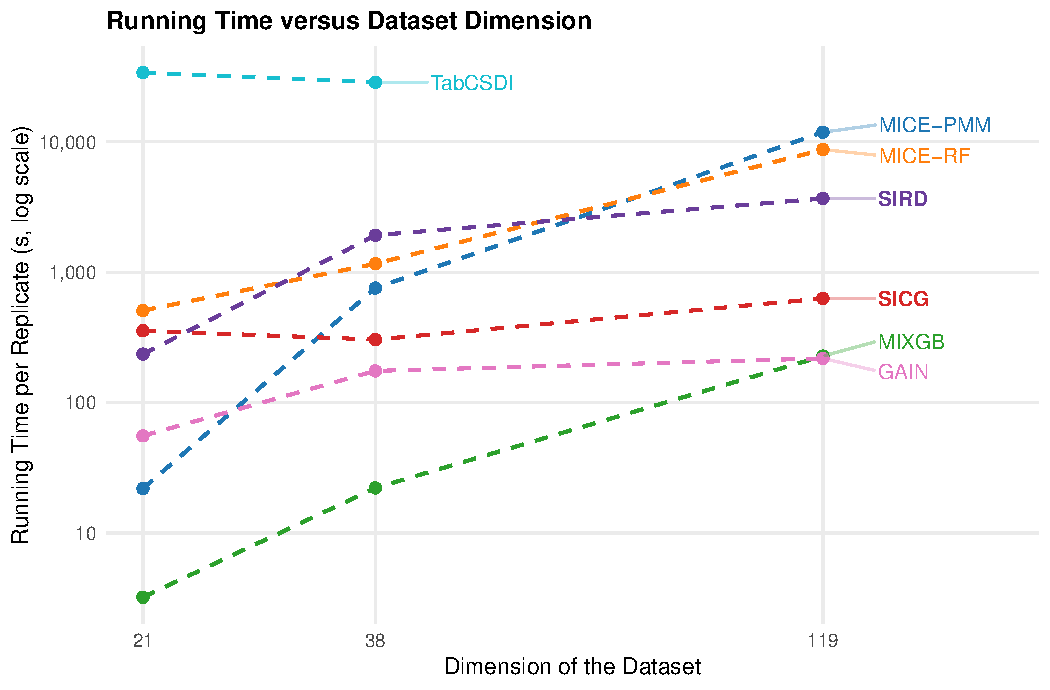
\includegraphics[width=\textwidth]{runtime_vs_dimensionality.pdf}
\caption{Median per-replicate running time in the three comparator settings, plotted against dataset dimension on a base-ten logarithmic time axis. Dashed lines join results for the same method; SICG and SIRD are shown in bold. The settings differ in more than dimension, so the connecting lines are descriptive.}
\label{fig:runtime}
\end{figure}

\subsection{Final Deployed Configurations of the Comparators}
\label{app:config_comparators}

The R methods retain their full search grids and are tuned once per setting. GAIN is also tuned over its full grid in each setting. TabCSDI holds five lower-importance diffusion and architecture parameters fixed while tuning \texttt{lr}, \texttt{batch\_size} and \texttt{featureemb} per setting. The deployed configuration is the componentwise median of the non-dominated trials, except for the survival random forest, which uses the five-trial rule in Section~\ref{sec:tuning}. In Design~III, \texttt{ntree} and \texttt{mtry} are subsequently reduced manually as described below. Table~\ref{tab:config_comparators} records the deployed values in all four settings.

\begin{table}[ht]
\centering
\caption{Deployed comparator configurations. The R methods and GAIN use their full search spaces in each setting. TabCSDI holds five lower-importance parameters fixed and tunes the remaining three. Configurations use the componentwise rule in Section~\ref{sec:tuning}; the survival random forest uses the five-trial rule, followed in Design~III by documented manual reductions to the tree count and the number of candidate variables per split. The final survival TabCSDI configuration was not carried into the simulation because of running cost.}
\label{tab:config_comparators}
\setlength{\tabcolsep}{5pt}
\begin{tabular}{llrrrr}
\toprule
Method & Parameter & Design~I & Design~II & Design~III & VCCC \\
\midrule
\multicolumn{6}{l}{\textit{\texttt{mice.impute.pmm}}} \\
 & \texttt{mincor} & 0.0775 & 0.379 & 0.053 & 0.207 \\
 & \texttt{ridge} & 0.420 & 0.498 & 0.003 & 0.439 \\
\addlinespace[2pt]
\multicolumn{6}{l}{\textit{\texttt{mice.impute.rf}}} \\
 & \texttt{ntree} & 105 & 44 & 10 & 118 \\
 & \texttt{mtry} & 6 & 13 & 63 & 23 \\
 & \texttt{nodesize} & 13 & 8 & 8 & 20 \\
 & \texttt{sampsize\_ratio} & 0.800 & 0.759 & 0.768 & 0.223 \\
\addlinespace[2pt]
\multicolumn{6}{l}{\textit{\texttt{mixgb}} (\texttt{nrounds} set separately by \texttt{mixgb\_cv})} \\
 & \texttt{gamma} & 0.445 & 0.337 & 0.334 & 0.167 \\
 & \texttt{min\_child\_weight} & 4 & 5 & 3 & 4 \\
 & \texttt{eta} & 0.105 & 0.134 & 0.093 & 0.072 \\
 & \texttt{subsample} & 0.605 & 0.650 & 0.725 & 0.687 \\
 & \texttt{max\_depth} & 4 & 4 & 2 & 6 \\
 & \texttt{colsample\_bytree} & 0.845 & 0.689 & 0.625 & 0.552 \\
\addlinespace[2pt]
\multicolumn{6}{l}{\textit{GAIN}} \\
 & \texttt{hint\_rate} & 0.63 & 0.60 & 0.65 & 0.90 \\
 & \texttt{alpha} & 330 & 100 & 200 & 350 \\
 & \texttt{beta} & 30 & 80 & 30 & 60 \\
 & \texttt{batch\_size} & 32 & 64 & 128 & 32 \\
 & \texttt{lr} & $2.5\times10^{-2}$ & $10^{-2}$ & $5\times10^{-3}$ & $10^{-2}$ \\
 & \texttt{epochs} & 9000 & 10000 & 15000 & 37000 \\
\addlinespace[2pt]
\multicolumn{6}{l}{\textit{TabCSDI} (tuned per setting)} \\
 & \texttt{lr} & $3.5\times10^{-4}$ & $2\times10^{-4}$ & $4\times10^{-4}$ & $5\times10^{-4}$ \\
 & \texttt{batch\_size} & 32 & 32 & 32 & 128 \\
 & \texttt{featureemb} & 10 & 15 & 11 & 7 \\
 & \texttt{epochs} & 3000 & 3000 & 3000 & 3000 \\
\addlinespace[2pt]
\multicolumn{6}{l}{\footnotesize TabCSDI held fixed across settings (low importance): \texttt{channels}$=128$, \texttt{nheads}$=2$,} \\
\multicolumn{6}{l}{\footnotesize \texttt{layers}$=2$, \texttt{num\_steps}$=60$, \texttt{diffusion\_embedding\_dim}$=128$.} \\
\bottomrule
\end{tabular}
\end{table}

For Simulation Design~III, the deployed random-forest values \texttt{ntree}$=10$ and \texttt{mtry}$=63$ were set manually below the values returned by the tuning search to reduce computation while retaining predictor subsampling. The tuned \texttt{nodesize}$=8$ and \texttt{sampsize\_ratio}$=0.768$ were retained.

\subsection{The Manually-Specified Comparators}
\label{app:manual_comparators}

The comparators in Table~\ref{tab:config_comparators} are the ones that carry a tuning grid. Several further comparators have no tunable hyperparameter and are defined entirely by the model they fit; this subsection specifies them setting by setting, in the notation of the corresponding technical-details section. Four estimators recur in every setting and differ only in the target model and the surrogate they use. The oracle (VAL) fits the target model on the fully validated cohort, in which the phase-two variables are known for every unit. The naive-proxy estimator (UNVAL) fits the target model on the full phase-one cohort with the error-prone surrogate in place of the validated variable. The complete-case estimator (CC) fits the target model on the validated rows only. Generalized raking (RAKING) fits a design-weighted working imputation model for the validated variable, takes the influence functions of the target-model fit as calibration variables, calibrates the phase-two design weights to them by raking, and refits the target model on the calibrated design \citep{deville1992calibration, breslow1988logistic, lumley2011complex}. The informative-sampling design adds four multiple-imputation comparators specific to it; the other three settings use only these four recurring estimators. Every multiple-imputation comparator imputes the missing values $m = 20$ times and pools the target-model fits by Rubin's rules \citep{Rubin1987}.

\paragraph{Simulation Design~I (informative sampling).} The target model is the Gaussian regression
\begin{equation}
\label{eq:appb_analysis}
Y_i = \beta_0 + \beta_X X_i + Z_i^{\top}\boldsymbol{\beta}_Z + \varepsilon_i ,
\end{equation}
with estimand $\beta_X$, where $X_i$ is the validated exposure observed only when $R_i = 1$, $\tilde{X}_i$ the error-prone surrogate used by UNVAL, $Z_i$ the recorded covariates and $W_i = 1/\pi_i$ the released design weight. Beyond VAL, UNVAL, CC and raking, four multiple-imputation comparators impute $X_i$ from the Gaussian model
\begin{equation}
\label{eq:appb_impmodel}
X_i = \boldsymbol{\alpha}^{\top}\mathbf{w}_i + \eta_i , \qquad \eta_i \sim N(0, \sigma^2), \qquad \mathbf{w}_i = (1, \tilde{X}_i, Z_i^{\top}, Y_i)^{\top},
\end{equation}
differing only in how the released weight enters:
\begin{itemize}
\item \emph{NAIVE} fits \eqref{eq:appb_impmodel} by proper Bayesian least squares on the validated rows (\texttt{imp\_gaussian} with \texttt{weighted = FALSE}), ignoring the weight; it is the standard baseline that Chapter~\ref{chap:SISL} identifies as vulnerable under informative selection.
\item \emph{NAIVE+W} adds factor-coded $W_i$ to the design vector, testing the specific extension in which the released weight enters as a categorical predictor.
\item \emph{WLMI} fits \eqref{eq:appb_impmodel} by weighted least squares with case weights $w_i = W_i/\bar{W}$ equal to the normalised design weights $(1/\pi_i)/\overline{(1/\pi)}$, and propagates the parameter uncertainty by a Bayesian bootstrap rather than a normal-theory draw \citep{Rubin1987, bartlett2020bootstrap}.
\item \emph{SISL} regresses $\log(W_i - 1)$ on flexible bases of $X_i$ and $Y_i$ to obtain a fitted inclusion function $\pi(x,V)$. It fits \eqref{eq:appb_impmodel} with
\[
f_s(x\mid V)=\frac{\pi(x,V)f_p(x\mid V)}{\mathbb E_{f_p}\{\pi(X,V)\mid V\}},
\]
and draws an unvalidated value from the normalised nonselection density
\[
f_0(x\mid V)=\frac{\{1-\pi(x,V)\}f_p(x\mid V)}{1-\mathbb E_{f_p}\{\pi(X,V)\mid V\}}
\]
\citep{pfeffermann1999parametric}. Section~\ref{sec:SISLmethod} gives the full specification.
\end{itemize}

\paragraph{Simulation Design~II (Gaussian and Binomial).} The two target models are the Gaussian systolic-blood-pressure model~\eqref{eq:appb_sbp_model} and the Binomial hypertension model~\eqref{eq:appb_htn_model}, whose exposure is the validated log-sodium intake; the error-prone dietary surrogate, the recorded average intake, plays the role of $\tilde{X}_i$ for UNVAL. Only VAL, UNVAL, CC and raking are used. Raking's working imputation model is a design-weighted Gaussian regression of the validated intake on the surrogate, the covariates and the outcome, and its calibration variables are the influence functions of the two target models.

\paragraph{Simulation Design~III (survival).} The target model is the Cox proportional-hazards model~\eqref{eq:appb_cox_true}; the error-prone surrogate laboratory and covariate values, marked with an asterisk in Appendix~\ref{app:sim2}, play the role of $\tilde{X}_i$ for UNVAL. Only VAL, UNVAL, CC and raking are used here. Raking's calibration variables are the \texttt{dfbeta} influence functions of the Cox partial-likelihood fit.

\paragraph{VCCC case study.} The three target models are the Gaussian, Binomial and Cox models of \eqref{eq:app_vccc_gauss}--\eqref{eq:app_vccc_cox}; the non-validated registry measurements play the role of $\tilde{X}_i$ for UNVAL. Only VAL, UNVAL, CC and raking are used here. Raking is applied to each target model in turn.

\section{Final Configurations for the Proposed Methods}
\label{app:proposed_config}

The comparator and proposed-method protocols differ in scope. Each comparator is tuned once per setting on the reference sample specified above. The R methods and GAIN use their full search spaces. TabCSDI uses its full space for VCCC and the reduced higher-importance space for Simulation Designs~I--III. SICG and SIRD required structural ablations, comparisons of uncertainty procedures and continuous hyperparameter searches. Repeating that full development process in every setting was computationally impractical. Their retained configurations were therefore developed on the Design~III reference setting and then reused unchanged in Simulation Designs~I and~II and the VCCC case study. This evaluates how the selected configurations transfer without per-setting retuning. It does not claim equal tuning budgets across methods or identify the fixed configurations as optimal in every setting.

Method development had two stages. The ablations in Chapters~\ref{chap:SICG} and~\ref{chap:SIRD} selected the network and loss structure, the categorical diffusion choice, classifier-free guidance and the uncertainty procedure by downstream coefficient bias, RMSE and coverage. Continuous architecture and optimisation parameters were then tuned once on a simple-random-sample replicate from Design~III. Each trial used three-fold cross-validation, masked the phase-two variables in the held-out fold, and returned $(\mathcal L_{\mathrm{data}},\mathcal L_{\mathrm{dist}})$ to a multi-objective Optuna study \citep{Akiba2019}.

The Optuna record supplies non-dominated trials and parameter-importance scores. It did not emit the deployed SICG or SIRD configuration automatically. The recorded importances were used to identify the parameters that required close attention; the trial history and marginal combined losses then guided the final values. This step included investigator judgement and should not be presented as a single automatic Pareto rule. Reproduction of the reported study uses the exact configurations in Tables~\ref{tab:config_sicg} and~\ref{tab:config_sird}. Epochs, and the SWAG learning rate where applicable, were examined in separate one-parameter sweeps. The comparator configurations continue to follow the explicit componentwise rule stated at the start of the appendix.

\subsection{SICG}

The retained configuration of SICG is the unpacked Wasserstein GAN with gradient penalty \citep{gulrajani2017improved} combined with MC-dropout multiple imputation \citep{gal2016dropout}. The ablation of Chapter~\ref{chap:SICG} set aside discriminator packing \citep{lin2018pacgan}, the auxiliary reconstruction and moment-matching losses, and the alternative SWAG \citep{maddox2019simple} and bootstrap uncertainty mechanisms, keeping the simplest generator that did not worsen interval calibration. Table~\ref{tab:tune_sicg} reports the search space over which the architecture and optimisation parameters were tuned. The importance analysis identified the generator width, the dropout rate, the learning rate and the batch size as the largest recorded contributors, together accounting for roughly nine tenths of the importance mass, and these were the parameters taken from the Pareto front, at the width of $512$, the dropout of $0.5$, the learning rate of $4 \times 10^{-4}$ and the batch size of $400$ recorded in Table~\ref{tab:config_sicg}. The remaining parameters, including the number of hidden layers, the weight decay, the Gumbel-softmax temperature \citep{jang2017categorical} and the number of discriminator steps, carried little importance and were each set one at a time from the value with the marginally lower combined loss $\mathcal{L}_{\mathrm{data}} + \mathcal{L}_{\mathrm{dist}}$ across the trial history. The discriminator-step count, for example, settled at three, between the value of one used to seed the search and the four preferred by the single lowest-loss trial. The number of training epochs was tuned separately on a categorical grid, and the shortest budget was retained because longer schedules tended to overfit the small phase-two sample. Table~\ref{tab:config_sicg} lists the final deployed configuration.

\begin{table}[ht]
\centering
\caption{Search space for SICG. The packing degree is tuned only in the packed branch of the ablation; the deployed configuration is unpacked.}
\label{tab:tune_sicg}
\begin{tabularx}{\textwidth}{lll>{\raggedright\arraybackslash}X}
\toprule
Parameter & Type & Range & Role \\
\midrule
\multicolumn{4}{l}{\textit{Stage 1: Architecture and optimisation}} \\
\texttt{hidden\_dim} & power of 2 & $\{64, \ldots, 1024\}$ &
    Generator and discriminator width. \\
\texttt{layers} & integer & $[1,\; 4]$ &
    Number of hidden layers. \\
\texttt{dropout} & continuous & $[0,\; 0.5]$ &
    Dropout rate, also the source of MC-dropout variability. \\
\texttt{lr} & log-uniform & $[10^{-4},\; 5 \times 10^{-3}]$ &
    Adam learning rate (generator and discriminator). \\
\texttt{batch\_size} & integer & $\{100, 200, \ldots, 500\}$ &
    Mini-batch size. \\
\texttt{weight\_decay} & log-uniform & $[10^{-6},\; 10^{-3}]$ &
    Adam weight decay. \\
\texttt{discriminator\_steps} & integer & $[1,\; 5]$ &
    Critic updates per generator step. \\
\texttt{tau} & continuous & $[0.1,\; 0.5]$ &
    Gumbel-softmax temperature. \\
\texttt{pack} & integer & $[2,\; 10]$ &
    Packing degree (packed branch only). \\
\midrule
\multicolumn{4}{l}{\textit{Stage 2: Training duration}} \\
\texttt{epochs} & categorical & $\{2500, \ldots, 20000\}$ &
    Number of training epochs. \\
\bottomrule
\end{tabularx}
\end{table}

\begin{table}[ht]
\centering
\caption{Final deployed configuration for SICG, reused without modification across all three simulation designs and the case study.}
\label{tab:config_sicg}
\begin{tabularx}{\textwidth}{ll>{\raggedright\arraybackslash}X}
\toprule
Parameter & Value & Role \\
\midrule
\multicolumn{3}{l}{\textit{Data processing}} \\
\texttt{normalization} & z-score & Column-wise standardisation. \\
\texttt{log} & true & Log transform of skewed variables. \\
\midrule
\multicolumn{3}{l}{\textit{Generator}} \\
\texttt{noise\_dim} & 64 & Latent noise dimension. \\
\texttt{hidden\_dim} & 512 & Hidden width. \\
\texttt{layers} & 2 & Hidden layers. \\
\texttt{dropout} & 0.5 & Dropout rate. \\
\midrule
\multicolumn{3}{l}{\textit{Discriminator}} \\
\texttt{hidden\_dim} & 512 & Hidden width. \\
\texttt{layers} & 2 & Hidden layers. \\
\texttt{pack} & 1 & Unpacked. \\
\midrule
\multicolumn{3}{l}{\textit{Multiple imputation}} \\
\texttt{m} & 20 & Number of imputations. \\
\texttt{mi\_approx} & MC-dropout & Between-imputation variance mechanism. \\
\midrule
\multicolumn{3}{l}{\textit{Training and optimisation}} \\
\texttt{epochs} & 2500 & Training epochs. \\
\texttt{batch\_size} & 400 & Mini-batch size. \\
\texttt{lr\_g}, \texttt{lr\_d} & $4 \times 10^{-4}$ &
    Adam learning rates, with $\beta = (0.5, 0.9)$. \\
\texttt{weight\_decay} & $10^{-6}$ & Adam weight decay. \\
\texttt{discriminator\_steps} & 3 & Critic updates per generator step. \\
\texttt{lambda\_gp} & 10 & Gradient-penalty weight. \\
\texttt{tau} & 0.2 & Gumbel-softmax temperature. \\
auxiliary losses & 0 &
    Reconstruction, cross-entropy, moment-matching and information losses disabled. \\
\bottomrule
\end{tabularx}
\end{table}

\subsection{SIRD}

The retained configuration of SIRD is the multinomial diffusion backbone \citep{hoogeboom2021multinomial} within the residual tabular denoising formulation \citep{kotelnikov2023tabddpm, ho2020denoising}, combined with bootstrap multiple imputation \citep{bartlett2020bootstrap}. The ablation of Chapter~\ref{chap:SIRD} discarded the analog-bits categorical encoding and did not retain classifier-free guidance \citep{ho2022classifier}, since the guided branch did not improve the downstream inferential diagnostics relative to the unguided backbone; the MC-dropout \citep{gal2016dropout} and SWAG \citep{maddox2019simple} mechanisms were examined and also set aside. Table~\ref{tab:tune_sird} reports the search space. The importance is concentrated in a single parameter to an unusual degree. The endpoint perturbation budget \texttt{sum\_scale}, which fixes the total noise variance added by the diffusion schedule, accounts for roughly one half of the importance mass, far above every other parameter. It was therefore treated as the one high-importance parameter, and its value, at the low end of its range, was read from the Pareto front. All of the remaining architecture and optimisation parameters carried low importance and were each set one at a time from the value with the marginally lower combined loss $\mathcal{L}_{\mathrm{data}} + \mathcal{L}_{\mathrm{dist}}$, as for SICG; the numeric and categorical loss weights, in particular, were of negligible importance and were held at unity. The number of diffusion steps was kept at the smallest value for which the tuning loss was still effectively flat, so that a coarser and cheaper reverse process could be used with no measurable penalty in fit. The number of training epochs was tuned on a separate categorical grid. Table~\ref{tab:config_sird} lists the final deployed configuration.

\begin{table}[ht]
\centering
\caption{Search space for SIRD. The guidance parameters are tuned only in the classifier-free-guidance branch of the ablation; the deployed configuration is unguided.}
\label{tab:tune_sird}
\begin{tabularx}{\textwidth}{lll>{\raggedright\arraybackslash}X}
\toprule
Parameter & Type & Range & Role \\
\midrule
\multicolumn{4}{l}{\textit{Stage 1: Diffusion, architecture and optimisation}} \\
\texttt{sum\_scale} & continuous & $[0.01,\; 0.25]$ &
    Terminal noise-variance budget of the schedule. \\
\texttt{num\_steps} & integer & $[20,\; 100]$ &
    Number of diffusion steps. \\
\texttt{diffusion\_embedding\_dim} & power of 2 & $\{64, 128, 256\}$ &
    Diffusion time-embedding dimension. \\
\texttt{channels} & power of 2 & $\{128, \ldots, 1024\}$ &
    Residual-block width. \\
\texttt{layers} & integer & $[2,\; 7]$ &
    Number of residual blocks. \\
\texttt{lr} & log-uniform & $[10^{-4},\; 10^{-2}]$ &
    AdamW learning rate. \\
\texttt{batch\_size} & power of 2 & $\{32, \ldots, 256\}$ &
    Mini-batch size. \\
\texttt{weight\_decay} & log-uniform & $[10^{-6},\; 10^{-3}]$ &
    AdamW weight decay. \\
\midrule
\multicolumn{4}{l}{\textit{Guidance branch (not deployed)}} \\
\texttt{cond\_drop\_prob} & continuous & $[0.05,\; 0.20]$ &
    Conditioning-dropout probability. \\
\texttt{cfg\_scale\_num}, \texttt{cfg\_scale\_cat} & continuous & $[1,\; 2]$ &
    Guidance scales for numeric and categorical variables. \\
\midrule
\multicolumn{4}{l}{\textit{Stage 2: Training duration}} \\
\texttt{epochs} & categorical & $\{2500, \ldots, 20000\}$ &
    Number of training epochs. \\
\bottomrule
\end{tabularx}
\end{table}

\begin{table}[ht]
\centering
\caption{Final deployed configuration for SIRD, reused without modification across all three simulation designs and the case study.}
\label{tab:config_sird}
\begin{tabularx}{\textwidth}{ll>{\raggedright\arraybackslash}X}
\toprule
Parameter & Value & Role \\
\midrule
\multicolumn{3}{l}{\textit{Data processing}} \\
\texttt{normalization} & z-score & Column-wise standardisation. \\
\texttt{log} & true & Log transform of skewed variables. \\
\midrule
\multicolumn{3}{l}{\textit{Diffusion}} \\
\texttt{task} & Res-N & Residual denoising target. \\
\texttt{discrete} & Multinomial & Categorical diffusion kernel. \\
\texttt{diffusion\_embedding\_dim} & 256 & Time-embedding dimension. \\
\texttt{num\_steps} & 25 & Diffusion steps. \\
\texttt{sum\_scale} & 0.01 & Terminal noise-variance budget. \\
\midrule
\multicolumn{3}{l}{\textit{Denoising network}} \\
\texttt{net} & ResNet & Residual multilayer denoiser. \\
\texttt{channels} & 256 & Residual-block width. \\
\texttt{layers} & 6 & Residual blocks. \\
\texttt{loss\_num}, \texttt{loss\_cat} & 1 & Numeric and categorical loss weights. \\
\midrule
\multicolumn{3}{l}{\textit{Multiple imputation}} \\
\texttt{m} & 20 & Number of imputations. \\
\texttt{mi\_approx} & Bootstrap & Between-imputation variance mechanism. \\
guidance & disabled & Classifier-free guidance scales set to zero. \\
\midrule
\multicolumn{3}{l}{\textit{Training and optimisation}} \\
\texttt{epochs} & 5000 & Training epochs. \\
\texttt{patience} & 2000 & Early-stopping patience. \\
\texttt{batch\_size} & 128 & Mini-batch size. \\
\texttt{lr} & $2 \times 10^{-4}$ & AdamW learning rate. \\
\texttt{weight\_decay} & $5 \times 10^{-4}$ & AdamW weight decay. \\
\bottomrule
\end{tabularx}
\end{table}

For both methods the only parameter that differs between the ablation configurations of Chapters~\ref{chap:SICG} and~\ref{chap:SIRD} and the deployed configurations above is the number of imputations, which is raised from five to twenty so that SICG and SIRD are pooled under Rubin's rules on the same number of completed datasets as the comparators \citep{Rubin1987, deng2024multiple}. The configurations in Tables~\ref{tab:config_sicg} and~\ref{tab:config_sird} are those loaded by every SICG and SIRD run reported in this thesis.

\section{Simulation Design I: Technical Details}
\label{app:infsamp}

This section documents the data-generating process and the sampling design used for the informative-sampling study of Chapter~\ref{chap:SISL}, described at a high level in Section~\ref{sec:infsamp_context}.

\subsection{Data generation}

A population of $N = 10{,}000$ individuals is generated under $500$ independent seeds. Two suppressed design variables are drawn independently and uniformly, $S_1, S_2 \in \{1, 2, 3\}$, and three recorded covariates are drawn as $Z_1, Z_2 \sim \mathcal{N}(0, 1)$ and $Z_3 \sim \mathrm{Bernoulli}(0.5)$. The stratum mean and the within-stratum standard deviations of $X$ and $Y$ are
\begin{equation}
m_{s_1 s_2} = a_{1, s_1} + a_{2, s_2}, \quad
\sigma^X_{s_1 s_2} = s_0 + s_1 (m_{s_1 s_2} - m_{\min}), \quad
\sigma^Y_{s_1 s_2} = s_0^Y + s_1^Y (m_{s_1 s_2} - m_{\min}),
\end{equation}
with $m_{\min} = \min_{s_1, s_2} m_{s_1 s_2}$. The validated measurement, the surrogate and the outcome are then generated by equations~\eqref{eq:infsamp_X}--\eqref{eq:infsamp_Y} with independent standard normal errors $\varepsilon^X_i, \tilde{\varepsilon}_i, \varepsilon^Y_i$. The parameter values are $a_1 = (-0.45,\, 0,\, 0.60)$, $a_2 = (-0.35,\, 0,\, 0.45)$, $s_0 = 0.30$, $s_1 = 0.58$, $s_0^Y = 0.30$, $s_1^Y = 0.70$, $\gamma = (0.18,\, 0.12,\, 0.14)$, $\alpha = 1.0$, $\delta = (0.40,\, 0,\, 0.50)$, $\tilde{\sigma} = 1.90$, $\beta_X = 0.48$ and $\beta = (0.30,\, 0.20,\, 0.30)$. The variance-mean coupling $s_1 > 0$ ties the within-stratum spread of $X$ to the stratum location. The surrogate has no direct $S_1$ or $S_2$ term, but it inherits information about them through $X$. Its large additional noise makes it only moderately informative about the validated measurement.

\subsection{Sampling design (\texttt{InfSamp})}

The nine combinations of $(S_1,S_2)$ are crossed with three empirical tertiles of the fully observed outcome $Y$, producing 27 joint sampling strata indexed by $h$. Under the budget $\sum_h n_h=n=500$, allocation follows $n_h\propto N_hs_h^Y$, where $N_h$ and $s_h^Y$ are the size and outcome standard deviation of joint stratum $h$. Within each joint stratum, $n_h$ individuals are selected by simple random sampling without replacement, so $\pi_i=n_h/N_h$ is positive and constant. The released data contain $(\tilde{X}_i,Z_i,Y_i)$, the selection indicator $R_i$, and the design weight $W_i=N_h/n_h=1/\pi_i$ for every individual; $X_i$ is retained only when $R_i=1$. The joint-stratum label and the variables $S_1$ and $S_2$ are not released. Thus the outcome component of the design is observed, while the stratifying variables that complete the sampling stratum remain hidden.

\section{Simulation Design II: Technical Details}
\label{app:sim1}
This section documents the data structure, measurement-error model and target models for Simulation Design~II, described in \ref{sec:sim1context}.
\subsection{Data Structure and Measurement Error Model}
\label{app:sim1_data}

Following the notation of Chapter~\ref{chap:background}, each individual $i$ has a vector of fully observed covariates $Z_i$ comprising centred age $\tilde{A}_i$, centred BMI $\tilde{B}_i$, sex indicator $F_i$, United States nativity status $U_i$, high total cholesterol indicator $C_i$, and ethnic background indicators $P_i$ (Puerto Rican) and $O_i$ (other). The error-prone phase-one dietary auxiliary vector is
\begin{equation}
    \tilde{X}_i \;=\; \bigl(
        \tilde{X}_i^{(\mathrm{Na})},\;
        \tilde{X}_i^{(\mathrm{K})},\;
        \tilde{X}_i^{(\mathrm{kcal})},\;
        \tilde{X}_i^{(\mathrm{prot})}
    \bigr)^{\top},
    \label{eq:app_phase1_aux}
\end{equation}
representing self-reported log-scale intakes of sodium, potassium, kilocalories, and protein, fully observed for all $N = 10{,}000$ individuals. The corresponding true dietary intake vector is
\begin{equation}
    X_i \;=\; \bigl(
        X_i^{(\mathrm{Na})},\;
        X_i^{(\mathrm{K})},\;
        X_i^{(\mathrm{kcal})},\;
        X_i^{(\mathrm{prot})}
    \bigr)^{\top},
    \label{eq:app_phase2_target}
\end{equation}
constituting the phase-two target variables, observed only for individuals with $R_i = 1$.

The original design of \citet{baldoni2021use} involves a three-tier measurement error structure in which the true intake $X_i$ is related to the self-reported intake $\tilde{X}_i$ through a linear Gaussian calibration model, and a biomarker $X^{**}_i = X_i + \varepsilon_i$ with $\varepsilon_i \sim \mathcal{N}(0, \sigma^2_\varepsilon)$ is additionally observed in the phase-two subsample. In the present study, the biomarker tier is removed; $X^{**}_i$ is generated but immediately discarded, and $X_i$ is treated directly as the phase-two target. The measurement error model for each component of $X_i$ retains the parametric form of \citet{baldoni2021use}. For log sodium,
\begin{equation}
    X_i^{(\mathrm{Na})} \;=\; \gamma_0
    + \gamma_1 \tilde{X}_i^{(\mathrm{Na})}
    + \gamma_2^{\top} Z_i
    + \delta_i^{(\mathrm{Na})},
    \qquad
    \delta_i^{(\mathrm{Na})} \;\sim\;
    \mathcal{N}\!\left(0,\, \sigma^2_{X,\mathrm{Na}}\right),
    \label{eq:app_meas_error_na}
\end{equation}
where $\sigma^2_{X,\mathrm{Na}} = \sigma^2_{\mathrm{Na}} - \sigma^2_{\varepsilon,\mathrm{Na}}$, with $\sigma^2_{\mathrm{Na}}$ the total variance and $\sigma^2_{\varepsilon,\mathrm{Na}}$ the biomarker error variance attenuated by a factor of $0.575$ relative to the SOLNAS estimates to ensure $\sigma^2_{X,\mathrm{Na}} > \sigma^2_{\varepsilon,\mathrm{Na}}$ \citep{baldoni2021use}. Analogous models are specified for log potassium, log kilocalories, and log protein. The coefficient $\gamma_1$ on the naive intake was inflated by a factor of $3$ for log sodium, $2$ for log potassium, and $2.5$ for log kilocalories and log protein relative to the SOLNAS estimates. This inflation was applied in \citet{baldoni2021use} to ensure that the surrogate $\tilde{X}_i$ carries sufficient information about the truth $X_i$ for the two-phase design to be effective at small sampling fractions.

\begin{table}[ht]
\centering
\caption{Gaussian linear model coefficients and variance parameters used to simulate the log-transformed true dietary intakes, reproduced from \citet{baldoni2021use}.}
\label{tab:app_meas_coef}
\begin{tabular}{lrrrr}
\hline
Coefficient & Log-sodium & Log-potassium & Log-energy & Log-protein \\
\hline
Intercept & 8.390 & 7.939 & 7.880 & 4.677 \\
Naive intake (centred) & 0.371 & 0.412 & 0.159 & 0.256 \\
Age (centred) & 0.001 & 0.006 & $-$0.001 & 0.001 \\
BMI (centred) & 0.018 & 0.012 & 0.015 & 0.017 \\
Female & $-$0.144 & $-$0.089 & $-$0.112 & $-$0.111 \\
Puerto Rican & $-$0.064 & $-$0.184 & 0.035 & $-$0.113 \\
Other background & 0.009 & 0.038 & 0.026 & 0.018 \\
Hypercholesterolaemia & $-$0.016 & $-$0.066 & $-$0.004 & $-$0.043 \\
Nativity & $-$0.086 & $-$0.036 & 0.025 & $-$0.089 \\
\hline
$\sigma^2$ & 0.220 & 0.174 & 0.021 & 0.100 \\
$\sigma^2_X$ & 0.123 & 0.089 & 0.016 & 0.055 \\
$\sigma^2_\varepsilon$ & 0.097 & 0.085 & 0.005 & 0.045 \\
\hline
\end{tabular}
\end{table}

\subsubsection{Target Outcome Models}
The original outcome model coefficients of \citet{baldoni2021use} are retained as the base specification, with two modifications. First, an interaction term $X_i^{(\mathrm{Na})} \cdot Z_i^{(\mathrm{AGE})}$ is added to both models. Second, the intercepts are recalibrated to achieve a marginal SBP mean of approximately $120\,\mathrm{mmHg}$ and a marginal hypertension prevalence of approximately $8\%$, compared to $122\,\mathrm{mmHg}$ and $10\%$ in the original. The first target model is a Gaussian model for systolic blood pressure,
\begin{align}
    Y_i^{(\mathrm{sbp})} \;=\; \beta_0
    &+ \beta_1 Z_i^{(\mathrm{AGE})}
    + \beta_2 Z_i^{(\mathrm{BMI})}
    + \beta_3 X_i^{(\mathrm{Na})}
    + \beta_4 Z_i^{(\mathrm{CHOL})}
    + \beta_5 Z_i^{(\mathrm{BORN})}
    + \beta_6 Z_i^{(\mathrm{SEX})} \nonumber \\
    &+ \beta_7 Z_i^{(\mathrm{PR})}
    + \beta_8 Z_i^{(\mathrm{OTH})}
    + \beta_9 \bigl(X_i^{(\mathrm{Na})} \cdot Z_i^{(\mathrm{AGE})}\bigr)
    + \varepsilon_i,
    \label{eq:appb_sbp_model}
\end{align}
with $\varepsilon_i \sim \mathcal{N}(0,\, \sigma^2)$, $\sigma^2 = 145.740$, and true interaction coefficient $\beta_9 = 0.15$. The remaining coefficients are given in Table~\ref{tab:app_outcome_coef}. The second target model is a Binomial model for hypertension status $Y_i^{(\mathrm{htn})} \in \{0,1\}$,
\begin{align}
    \log \frac{\Pr(Y_i^{(\mathrm{htn})} = 1)}{%
              1 - \Pr(Y_i^{(\mathrm{htn})} = 1)}
    \;=\; \alpha_0
    &+ \alpha_1 Z_i^{(\mathrm{AGE})}
    + \alpha_2 Z_i^{(\mathrm{BMI})}
    + \alpha_3 X_i^{(\mathrm{Na})}\nonumber \\
    &+ \alpha_4 Z_i^{(\mathrm{CHOL})}
    + \alpha_5 Z_i^{(\mathrm{BORN})}
    + \alpha_6 Z_i^{(\mathrm{SEX})}\nonumber \\
    &+ \alpha_7 Z_i^{(\mathrm{PR})}
    + \alpha_8 Z_i^{(\mathrm{OTH})}
    + \alpha_9 \bigl(X_i^{(\mathrm{Na})} \cdot Z_i^{(\mathrm{AGE})}\bigr),
    \label{eq:appb_htn_model}
\end{align}
with true interaction coefficient $\alpha_9 = 0.005$. The remaining coefficients are given in Table~\ref{tab:app_outcome_coef}.

\begin{table}[ht]
\centering
\caption{Outcome model coefficients used in the present simulation study. Base coefficients are reproduced from \citet{baldoni2021use}; intercepts are recalibrated and interaction coefficients are added in the present study.}
\label{tab:app_outcome_coef}
\begin{tabular}{lrr}
\hline
Coefficient & SBP ($\hat{\beta}$) & Hypertension ($\hat{\alpha}$) \\
\hline
Intercept (recalibrated) & 120.000 (approx.) & $-$2.340 (approx.) \\
Log-sodium (centred) & 27.473 & 1.439 \\
Age (centred) & 0.406 & 0.087 \\
BMI (centred) & 0.170 & 0.056 \\
Female & $-$8.932 & $-$0.120 \\
Puerto Rican & $-$1.670 & $-$0.175 \\
Other background & $-$2.322 & $-$0.845 \\
Hypercholesterolaemia & 1.611 & 0.379 \\
Nativity & $-$0.564 & $-$0.220 \\
Interaction (Na $\times$ Age) & 0.150 & 0.005 \\
$\sigma^2$ & 145.740 & --- \\
\hline
\end{tabular}
\end{table}

\subsection{Sampling Designs}
\label{app:sim1_sampling}

Seven sampling designs are applied to each of the $500$ simulated populations to draw the phase-two validation sample of size $n = 500$. For each design, the selection indicator $R_i \in \{0,1\}$ is defined, $X_i$ is masked for all individuals with $R_i = 0$, and sampling weights $W_i$ are assigned according to the design. The probability designs (\texttt{SRS}, \texttt{Neyman-ODS}, \texttt{Neyman-IF}) admit a positive inclusion probability $\pi_i$ for every unit and carry the design weight $W_i = 1/\pi_i$, which the design-based estimators require; the tail-based designs (\texttt{RS}, \texttt{WRS}, \texttt{SFS}, \texttt{ODS-Tail}) select units deterministically from the extremes of a phase-one score and do not define a positive inclusion probability for every unit, so no design weights are available for them and they are analysed unweighted. Unless otherwise stated, all $W_i = 1$.

\subsubsection{Design 1: Simple Random Sampling (\texttt{SRS})}

Each individual is selected independently with equal inclusion probability $\pi_i = n/N = 0.05$, so the design weight $W_i = 1/\pi_i = N/n = 20$ is constant across units and the weighted analysis coincides with the unweighted one. \texttt{SRS} serves as the na\"ive unweighted baseline and represents the most common validation design used in measurement-error practice \citep{amorim2021two}.

\subsubsection{Design 2: Residual Sampling (\texttt{RS})}

A phase-one linear model for $Y^{(\mathrm{sbp})}$ is fitted using $Z_i$ and $\tilde{X}_i$ jointly. Residuals $\hat{e}_i$ are computed for all $N$ individuals. The $n/2$ individuals with the most extreme positive residuals and the $n/2$ with the most extreme negative residuals are selected deterministically.

For model-based estimators, residual sampling directs validation towards observations whose outcomes are poorly predicted by the phase-one covariates. \citet[Sections~3 and~5]{amorim2021two} show that it performs similarly to the locally optimal weighted-residual design when $\beta$ is close to zero and $\operatorname{Var}(X\mid X^*,Z)$ is constant across $Z$.

\subsubsection{Design 3: Weighted Residual Sampling (\texttt{WRS})}

\citet{tao2019optimal} derived the optimal model-based design under the local alternative $\beta = o(1)$: phase-two selection should maximise $(Y_i - \mu(Z_i))^2 \operatorname{Var}(X_i \mid X^*_i, Z_i)$, where $\mu(Z_i)$ is the linear predictor from a regression of $Y$ on $Z$ alone. The factor $\operatorname{Var}(X \mid X^*, Z)$ up-weights individuals whose error-prone measurements are least informative about the truth; when this variance is approximately constant across covariate levels, \texttt{WRS} reduces to residual sampling \citep[Section~3.1]{amorim2021two}. Because $\operatorname{Var}(X \mid X^*, Z)$ is unknown from phase-one data alone, a pilot subsample of size $n_{\mathrm{pilot}} = \lfloor 0.1 \times n \rfloor = 50$ is drawn by simple random sampling from the $N$ phase-one individuals. A pilot regression of $X^{(\mathrm{Na})}$ on $Z_i$ and $\tilde{X}_i$ is fitted to this subsample, yielding the residual standard deviation $\hat{\sigma}_{\mathrm{pilot}}$. For the remaining $N - n_{\mathrm{pilot}}$ individuals, a phase-one model for $Y^{(\mathrm{sbp})}$ on $Z_i$ alone is fitted and its residuals $\hat{e}^*_i$ are scaled to form $\tilde{e}_i = \hat{e}^*_i \cdot \hat{\sigma}_{\mathrm{pilot}}$. The remaining $n - n_{\mathrm{pilot}}$ individuals are drawn from the tails of $\tilde{e}_i$, and the pilot subsample is combined to complete the phase-two cohort.

\subsubsection{Design 4: Score Function Sampling (\texttt{SFS})}

A phase-one linear model for $Y^{(\mathrm{sbp})}$ is fitted on $Z_i$ only, excluding $\tilde{X}_i$. The empirical score contribution for the sodium coefficient is approximated as $s_i = \hat{e}_i \cdot \tilde{X}_i^{(\mathrm{Na})}$, where $\hat{e}_i$ is the model residual. The $n/2$ individuals with the most extreme positive and negative values of $s_i$ are selected.

\citet{amorim2021two} propose \texttt{SFS} as a practical alternative to \texttt{WRS}: it avoids the need for a pilot sample or prior knowledge of $\operatorname{Var}(X \mid X^*, Z)$ by substituting the error-prone covariate $X^*$ directly into the score expression. \texttt{SFS} therefore selects individuals using the product of the phase-one residual and the surrogate covariate. Simulations in \citet[Table~1]{amorim2021two} show that \texttt{SFS} outperforms \texttt{RS} and \texttt{WRS} when $\beta$ deviates substantially from zero and $X^*$ is a fair surrogate for $X$.

\subsubsection{Design 5: Outcome-Dependent Sampling by Tails (\texttt{ODS-Tail})}

The $n/2$ individuals at the lower extreme and the $n/2$ at the upper extreme of the $Y^{(\mathrm{sbp})}$ distribution are deterministically selected. Outcome-dependent sampling exploits the fact that subjects in the tails of the outcome distribution exert greater influence on the regression parameter; by oversampling them, one expects to increase efficiency for model-based estimators \citep{zhou2002semiparametric, amorim2021two}.

\subsubsection{Design 6: Outcome-Dependent Sampling by Neyman Allocation (\texttt{Neyman-ODS})}

The distribution of $Y^{(\mathrm{sbp})}$ is partitioned into three strata at the 19th and 81st empirical percentiles. Within stratum $k$, the phase-two allocation is $n_k \propto N_k \hat{S}_k$, where $N_k$ is the stratum size and $\hat{S}_k$ is the within-stratum standard deviation of the phase-one sodium proxy $\tilde{X}_i^{(\mathrm{Na})}$. For this allocation variable, the Neyman criterion minimises the design variance of its Horvitz--Thompson total at a fixed sample size \citep{neyman1938contribution}. It is an auxiliary-variable Neyman allocation; Design~7 instead bases the allocation on an approximate influence function for a regression coefficient. Sampling weights are set to $W_i = N_k / n_k$ for all individuals in stratum~$k$ \citep{Weaver2005, lumley2011connections}.

\subsubsection{Design 7: Influence Function Sampling by Neyman Allocation (\texttt{Neyman-IF})}

The same three $Y^{(\mathrm{sbp})}$-based strata from Design~6 are retained. For each individual $i$, the approximate influence $\mathrm{h}_i(\hat{\beta})$ on the $\tilde{A}$ coefficient is computed via the \texttt{dfbeta} approximation applied to the phase-one model for $Y^{(\mathrm{sbp})}$ augmented by $\tilde{X}_i^{(\mathrm{Na})}$ and its interaction with $\tilde{A}_i$. The Neyman allocation within strata is driven by the within-stratum standard deviation of $\mathrm{h}_i(\hat{\beta})$.

\citet[Section~4.1]{amorim2021two} prove that for IPW estimators the optimal phase-two allocation from stratum~$k$ satisfies $n_k / n = N_k s_k / \sum_{k'} N_{k'} s_{k'}$, where $s_k$ is the standard deviation of the influence function for $\hat{\beta}$ within stratum~$k$. Because $\hat{\beta}_w$ is asymptotically equivalent to a sum of influence functions \citep[eq.~10]{amorim2021two}, this result is the direct translation of classical Neyman allocation from the population-total setting to two-phase regression \citep{lumley2011connections, mcisaac2014response}. The influence function is approximated by replacing the unobserved $X_i$ with the error-prone $\tilde{X}_i$; \citet{amorim2021two} recommend that this approximation be highly correlated with the true influence function (following the $r \geq 0.90$ rule of thumb of \citealt{sarndal1992model}). Sampling weights are set to $W_i = N_k / n_k$.

For the two stratified probability designs, the realised per-stratum sampling fractions, averaged over the $500$ replicates, show how the fixed budget of $n = 500$ is distributed across strata. The three $Y^{(\mathrm{sbp})}$ strata, cut at the 19th and 81st percentiles with sizes $N_k \approx 1900$, $6200$ and $1900$, receive sampling fractions $n_k/N_k$ of approximately $0.051$, $0.050$ and $0.048$ under \texttt{Neyman-ODS}, so that this outcome-stratified allocation is close to proportional; under \texttt{Neyman-IF} the same strata receive approximately $0.070$, $0.038$ and $0.069$, concentrating the validation budget in the two outer strata, where the influence-function spread is largest. Under \texttt{SRS} every unit is sampled at the common fraction $0.05$.


\section{Simulation Design III: Technical Details}
\label{app:sim2}
This section documents the electronic-health-record parameter estimates, data structure and target model for Simulation Design~III, described in \ref{sec:sim2context}.
\subsection{Empirical Parameter Estimation from EHR Data}
\label{app:sim2_ehr}

The clinical laboratory parameters used in this simulation are estimated from a retrospective electronic health record cohort comprising $530{,}165$ emergency department presentations across two New Zealand metropolitan hospitals (North Shore Hospital and Waitakere Hospital) between July 2016 and June 2021. Key characteristics of the cohort include a mean age of $52.6$ years (SD $21.7$), $54.1\%$ female, and a hospital admission rate of approximately $40\%$.

For each laboratory panel, a race- and sex-stratified covariance matrix $\hat{\Sigma}$ is estimated from the EHR data using pairwise complete observations, then projected to the nearest positive semi-definite matrix. The panels and their constituent variables are: renal (creatinine, urea, potassium, sodium, chloride, bicarbonate, calcium, magnesium, phosphate); hepatic (aspartate aminotransferase [AST], alanine aminotransferase [ALT], alkaline phosphatase [ALP], gamma-glutamyl transferase [GGT], bilirubin, albumin, globulin, total protein); haematology (haemoglobin [Hb], haematocrit [HCT], red and white blood cell counts [RBC and WBC], platelet count, mean corpuscular volume [MCV], red cell distribution width [RDW], neutrophils, lymphocytes, monocytes, eosinophils, basophils); lipids (triglycerides, high-density lipoprotein [HDL], low-density lipoprotein [LDL]); diabetic markers (glucose, fasting glucose, glycated haemoglobin [HbA1c], insulin); and vital signs (systolic blood pressure [SBP], temperature, heart rate, peripheral oxygen saturation [SpO2]).

For each variable within each panel, a generalised linear model regressing the variable on sex, race, age, BMI, smoking status, and medication count is fitted to the EHR data. Only predictors significant at $p < 0.05$ in the multivariable model are retained; non-significant predictors are set to zero in the simulation. To protect data privacy, independent Gaussian noise $\mathcal{N}(0, 0.05^2)$ is added to each race-specific regression coefficient before use in the simulation. The complete set of estimated coefficients and covariance matrices is fixed across all $500$ simulation replicates.

\subsection{Population Variable Generation}
\label{app:sim2_popgen}

Each simulated population of $N = 20{,}000$ individuals is generated sequentially in the order shown in Table~\ref{tab:app_sim2_overview}. All continuous laboratory outcomes are generated on the log scale and back-transformed via $\exp(\cdot) - 1$ before use. Multivariate panels are drawn jointly from a multivariate Gaussian distribution with empirically estimated covariance matrix $\hat{\Sigma}$ and conditional mean $\boldsymbol{\mu}_i = \hat{\boldsymbol{\gamma}}^{\top}\mathbf{c}_i$.

\begin{table}[ht]
\centering
\caption{Variable generation order, distribution family, predictor set, and back-transformation for each variable or group.}
\label{tab:app_sim2_overview}
\small
\begin{tabular}{p{3.2cm}p{3.2cm}p{4.9cm}p{1.5cm}}
\hline
\textbf{Variable / Group} & \textbf{Distribution} &
\textbf{Predictors} & \textbf{Transf.} \\
\hline
AGE & Trunc.\ Normal$(62,10^2)$, $[25,90]$ & None & No \\
SEX & Bernoulli$(0.55)$ & None & No \\
RACE & Multinomial & None & No \\
INSURANCE & Bernoulli$(0.70)$ & None & No \\
REGION & Categorical (20) & None & No \\
URBAN & Derived & REGION & No \\
INCOME & Categorical (5) & None & No \\
EDU & Poisson$(4)+6$ & None & No \\
15 SNP genotypes & Binomial, Hardy--Weinberg equilibrium & Race-specific minor allele frequencies and linkage disequilibrium & No \\
HEIGHT & Normal & SEX, rs11708067 & No \\
SMOKE & Multinomial logit & AGE, SEX, RACE & No \\
EXER & Multinomial logit & AGE, SEX, RACE, SMOKE & No \\
ALC & Multinomial logit & AGE, SEX, RACE, SMOKE, EXER & No \\
BMI & Log-Normal & SEX, SMOKE, RACE, AGE, 4 SNPs$^a$ & Yes \\
MARRIAGE & Multinomial logit & AGE, SEX, RACE, BMI & No \\
MED\_Count & Poisson log-linear & SEX, SMOKE, RACE, AGE, BMI & No \\
RENAL (9 vars) & Multiv. normal & Standard set$^b$ & Yes \\
LIPIDS (3 vars) & Multiv. normal & Standard set$^b$ & Yes \\
HEMA (12 vars) & Multiv. normal & Standard set$^b$ & Yes \\
NUTRIENTS (4 vars) & Multiv. normal & AGE, SEX, BMI, RACE & Yes \\
LIVER (8 vars) & Multiv. normal & Standard set$^b$ & Yes \\
DIABETE (4 vars) & Multiv. normal & Variable-specific$^c$ & Yes \\
FERRITIN & Log-Normal & SEX, SMOKE, RACE, AGE, MED\_Count & Yes \\
VITALS (4 vars) & Multiv. normal & Variable-specific$^c$ & Yes \\
WEIGHT & Derived & BMI, HEIGHT & No \\
Estimated glomerular filtration rate (eGFR) & Chronic Kidney Disease Epidemiology Collaboration (CKD-EPI) formula & Creatinine, AGE, SEX & No \\
\hline
\multicolumn{4}{l}{$^a$ SNPs: rs10811661, rs11708067, rs4506565, rs5219.} \\
\multicolumn{4}{l}{$^b$ Standard set: SEX, SMOKE, RACE, AGE, BMI, MED\_Count; some variables exclude} \\
\multicolumn{4}{l}{\phantom{$^b$} certain predictors; see Tables~\ref{tab:app_coef_renal}--\ref{tab:app_coef_liver}.} \\
\multicolumn{4}{l}{$^c$ Variable-specific predictors; see Tables~\ref{tab:app_coef_vitals} and~\ref{tab:app_coef_diabete}.} \\
\end{tabular}
\end{table}

\subsection{Regression Coefficients}
\label{app:sim2_coef}

The multivariate-normal blocks listed above, namely RENAL, LIPIDS, HEMA, NUTRIENTS, LIVER, DIABETE, and VITALS, are panels of correlated clinical measurements generated jointly and named for the physiological system they represent; for example, the DIABETE panel collects the glycaemic markers (non-fasting and fasting glucose, glycated haemoglobin, and insulin) and the LIPIDS panel the serum lipids (triglyceride, HDL, and LDL). Tables~\ref{tab:app_coef_scalar}--\ref{tab:app_coef_diabete} report the regression coefficients $\hat{\boldsymbol{\gamma}}$ for each variable group, with predictors as rows and outcome variables as columns. RACE categories are coded relative to European (EUR): RACE2~=~African (AFR), RACE3~=~Admixed American (AMR), RACE4~=~South Asian (SAS), and RACE5~=~East Asian (EAS). SMOKE categories are relative to Current Smoker. All SNP coefficients represent the per-allele additive effect. A dash (---) indicates the predictor was excluded at $p < 0.05$ in the EHR regression.

\begin{table}[ht]
\centering
\caption{Coefficients for scalar variables. Columns give (1)~height, (2)~body mass index on the log scale, (3)~medication count under a Poisson log-linear model, and (4)~ferritin on the log scale.}
\label{tab:app_coef_scalar}
\small
\begin{tabular}{lrrrr}
\hline
\textbf{Predictor} & \textbf{(1)} & \textbf{(2)} &
\textbf{(3)} & \textbf{(4)} \\
\hline
Intercept        & 162.000 &  3.383 & $-$0.334 &  3.073 \\
SEX              &  13.000 &  0.009 & $-$0.126 &  0.625 \\
SMOKE\_Ex        &     --- &  0.063 & $-$0.368 & $-$0.086 \\
SMOKE\_Nev       &     --- &  0.038 & $-$0.495 & $-$0.053 \\
RACE2 (AFR)      &     --- &  0.081 &    0.363 &  0.032 \\
RACE3 (AMR)      &     --- &  0.242 &    0.114 &  0.228 \\
RACE4 (SAS)      &     --- &  0.032 & $-$0.134 & $-$0.124 \\
RACE5 (EAS)      &     --- & $-$0.200 & $-$0.408 &  0.221 \\
AGE              &     --- & $-$0.0018 &  0.0180 &  0.0120 \\
BMI              &     --- &    --- &    0.693 &    --- \\
MED\_Count       &     --- &    --- &      --- & $-$0.001 \\
rs11708067       &   0.015 &  0.055 &      --- &    --- \\
rs10811661       &     --- &  0.027 &      --- &    --- \\
rs4506565        &     --- &  0.011 &      --- &    --- \\
rs5219           &     --- &  0.012 &      --- &    --- \\
\hline
\end{tabular}
\end{table}

\begin{table}[ht]
\centering
\caption{Coefficients for the vital-sign measurements on the log scale. Columns give (1)~systolic blood pressure, (2)~temperature, (3)~heart rate, and (4)~oxygen saturation.}
\label{tab:app_coef_vitals}
\small
\begin{tabular}{lrrrr}
\hline
\textbf{Predictor} & \textbf{(1)} & \textbf{(2)} & \textbf{(3)} & \textbf{(4)} \\
\hline
Intercept    &  4.3936 &  3.6311 &  4.3458 &  4.6071 \\
SEX          &  0.0083 & $-$0.0012 &     --- &  0.0003 \\
SMOKE\_Ex    & $-$0.0236 &  0.0006 & $-$0.0068 &  0.0002 \\
SMOKE\_Nev   & $-$0.0096 &  0.0013 & $-$0.0053 &  0.0019 \\
RACE2 (AFR)  & $-$0.0334 &  0.0346 & $-$0.0812 &  0.0308 \\
RACE3 (AMR)  & $-$0.0504 &  0.0520 & $-$0.0089 &  0.0683 \\
RACE4 (SAS)  &  0.0557 &  0.0918 &  0.0285 & $-$0.0078 \\
RACE5 (EAS)  & $-$0.0414 & $-$0.0400 &  0.0479 &  0.0895 \\
AGE          &     --- & $-$0.0000224 & $-$0.0006 & $-$0.0001 \\
BMI          &  0.0876 &  0.0009 &     --- & $-$0.0038 \\
MED\_Count   & $-$0.0006 &  0.0000086 &  0.0001 & $-$0.0000245 \\
rs5219       &  0.3200 &     --- &     --- &     --- \\
rs7754840    &  0.1800 &     --- &     --- &     --- \\
rs7756992    &  0.2075 &     --- &     --- &     --- \\
\hline
\end{tabular}
\end{table}

\begin{landscape}
\begin{table}[ht]
\centering
\caption{Coefficients for the renal measurements on the log scale. Columns give (1)~creatinine, (2)~urea, (3)~potassium, (4)~sodium, (5)~chloride, (6)~bicarbonate, (7)~calcium, (8)~magnesium, and (9)~phosphate. Dashes indicate a predictor excluded at $p < 0.05$.}
\label{tab:app_coef_renal}
\resizebox{\linewidth}{!}{%
\begin{tabular}{lrrrrrrrrr}
\hline
\textbf{Predictor} & \textbf{(1)} & \textbf{(2)} &
\textbf{(3)} & \textbf{(4)} & \textbf{(5)} & \textbf{(6)} &
\textbf{(7)} & \textbf{(8)} & \textbf{(9)} \\
\hline
Intercept    &  2.8712 &  0.3175 &  1.4837 &  4.9161 &  4.6337
             &  3.1565 &  1.1792 &  0.6138 &  0.6992 \\
SEX          &  0.2924 &  0.1955 &  0.0186 &  0.0018 & $-$0.0032
             &  0.0056 & $-$0.0061 &  0.0102 &     --- \\
SMOKE\_Ex    &  0.1065 &  0.1982 &  0.0057 &     --- &     ---
             & $-$0.0078 &  0.0022 &  0.0113 &  0.0187 \\
SMOKE\_Nev   &  0.0850 &  0.1580 &  0.0044 &     --- &     ---
             & $-$0.0083 &  0.0052 &  0.0193 &  0.0084 \\
RACE2 (AFR)  &  0.2296 &  0.3067 &  0.0439 & $-$0.0044 &  0.0321
             & $-$0.0901 & $-$0.0565 &  0.0141 &  0.0255 \\
RACE3 (AMR)  &  0.2816 &  0.3517 &  0.0086 &  0.1157 & $-$0.0639
             & $-$0.1041 &  0.0801 &  0.0710 &  0.1331 \\
RACE4 (SAS)  &  0.1041 &  0.1591 & $-$0.0036 &  0.0277 & $-$0.0559
             & $-$0.0125 &  0.0307 &  0.0460 & $-$0.0291 \\
RACE5 (EAS)  &  0.0138 &  0.1053 & $-$0.0435 & $-$0.0068 &  0.0210
             & $-$0.1142 &  0.0196 & $-$0.0179 &  0.0268 \\
AGE          &  0.0061 &  0.0110 &  0.0008 & $-$0.0002 & $-$0.0003
             &  0.0003 & $-$0.0001 & $-$0.0002 &     --- \\
BMI          &  0.2091 &  0.1880 &  0.0188 &  0.0080 &  0.0062
             &  0.0123 &  0.0039 & $-$0.0086 &     --- \\
MED\_Count   &  0.0025 &  0.0016 &  0.0002 & $-$0.0001 & $-$0.0001
             &  0.0002 &  0.0001 &     --- &  0.0007 \\
\hline
\end{tabular}}
\end{table}
\end{landscape}

\begin{table}[ht]
\centering
\caption{Coefficients for the lipid measurements on the log scale. Columns give (1)~triglyceride, (2)~high-density lipoprotein cholesterol, and (3)~low-density lipoprotein cholesterol.}
\label{tab:app_coef_lipids}
\small
\begin{tabular}{lrrr}
\hline
\textbf{Predictor} & \textbf{(1)} & \textbf{(2)} & \textbf{(3)} \\
\hline
Intercept    & $-$0.089 &  1.479 &  1.532 \\
SEX          &    0.041 & $-$0.100 & $-$0.055 \\
SMOKE\_Ex    & $-$0.029 &  0.000 & $-$0.031 \\
SMOKE\_Nev   & $-$0.065 &  0.012 & $-$0.003 \\
RACE2 (AFR)  & $-$0.040 & $-$0.025 &  0.047 \\
RACE3 (AMR)  & $-$0.053 & $-$0.056 & $-$0.108 \\
RACE4 (SAS)  &    0.055 & $-$0.063 &  0.012 \\
RACE5 (EAS)  &    0.098 &  0.010 & $-$0.133 \\
AGE          & $-$0.001 &  0.000 & $-$0.003 \\
BMI          &    0.317 & $-$0.154 &    --- \\
MED\_Count   &    0.001 & $-$0.000 & $-$0.001 \\
rs17036101   &    0.032 &    --- &    --- \\
rs7756992    &      --- &    --- &  0.020 \\
\hline
\end{tabular}
\end{table}

\begin{table}[ht]
\centering
\caption{Coefficients for the glycaemic measurements on the log scale. Columns give (1)~glucose, (2)~fasting glucose, (3)~glycated haemoglobin, and (4)~insulin. Insulin has one retained predictor, rs11708067.}
\label{tab:app_coef_diabete}
\small
\begin{tabular}{lrrrr}
\hline
\textbf{Predictor} & \textbf{(1)} & \textbf{(2)} & \textbf{(3)} & \textbf{(4)} \\
\hline
Intercept    &  1.1823 &  0.9513 &  2.5740 &  3.0134 \\
SEX          &  0.0507 &     --- &  0.0613 &     --- \\
SMOKE\_Ex    &     --- &     --- & $-$0.0125 &     --- \\
SMOKE\_Nev   &     --- &     --- & $-$0.0228 &     --- \\
RACE2 (AFR)  &  0.0506 &     --- &  0.1534 &     --- \\
RACE3 (AMR)  &  0.1770 &     --- &  0.1914 &     --- \\
RACE4 (SAS)  &  0.1484 &     --- &  0.0775 &     --- \\
RACE5 (EAS)  &  0.0782 &     --- &  0.0253 &     --- \\
AGE          &  0.0033 &     --- &  0.0035 &     --- \\
BMI          &  0.1546 &  0.2882 &  0.2575 &     --- \\
MED\_Count   &  0.0008 &     --- &  0.0012 &     --- \\
rs7756992    &  0.0340 &     --- &     --- &     --- \\
rs10811661   &     --- &  0.0297 &  0.0918 &     --- \\
rs11708067   &     --- &  0.0327 &  0.0523 &  0.0135 \\
rs4506565    &     --- &  0.0229 &     --- &     --- \\
\hline
\end{tabular}
\end{table}

\begin{table}[ht]
\centering
\caption{Coefficients for the dietary-intake measurements on the log scale. Columns give (1)~sodium intake, (2)~potassium intake, (3)~energy intake, and (4)~protein intake.}
\label{tab:app_coef_nutrients}
\small
\begin{tabular}{lrrrr}
\hline
\textbf{Predictor} & \textbf{(1)} & \textbf{(2)} & \textbf{(3)} & \textbf{(4)} \\
\hline
Intercept    &    7.660 &    7.200 &    7.400 &    4.000 \\
AGE          & $-$0.00084 &  0.00750 & $-$0.00256 &  0.00046 \\
SEX          &    0.270 &    0.177 &    0.160 &    0.187 \\
BMI          &    0.018 &    0.010 &    0.014 &    0.017 \\
RACE2 (AFR)  &    0.009 &    0.040 &    0.200 &    0.020 \\
RACE3 (AMR)  & $-$0.100 & $-$0.080 & $-$0.400 & $-$0.130 \\
RACE4 (SAS)  & $-$0.150 & $-$0.120 & $-$0.600 & $-$0.140 \\
RACE5 (EAS)  &    0.030 &    0.020 &    0.120 &    0.100 \\
\hline
\end{tabular}
\end{table}

\begin{landscape}
\begin{table}[ht]
\centering
\caption{Coefficients for the liver measurements on the log scale. Columns give (1)~aspartate aminotransferase, (2)~alanine aminotransferase, (3)~alkaline phosphatase, (4)~gamma-glutamyl transferase, (5)~bilirubin, (6)~albumin, (7)~globulin, and (8)~total protein. Dashes indicate a predictor excluded at $p < 0.05$.}
\label{tab:app_coef_liver}
\resizebox{\linewidth}{!}{%
\begin{tabular}{lrrrrrrrr}
\hline
\textbf{Predictor} & \textbf{(1)} & \textbf{(2)} & \textbf{(3)} & \textbf{(4)} &
\textbf{(5)} & \textbf{(6)} & \textbf{(7)} & \textbf{(8)} \\
\hline
Intercept    &  3.325 &  2.345 &  4.074 &  1.637
             &  1.823 &  3.731 &  3.304 &  4.204 \\
SEX          &  0.106 &  0.173 &  0.034 &  0.265
             &  0.207 &    --- &    --- &  0.002 \\
SMOKE\_Ex    & $-$0.107 & $-$0.027 & $-$0.031 & $-$0.080
             &  0.061 & $-$0.011 & $-$0.004 & $-$0.003 \\
SMOKE\_Nev   & $-$0.041 &  0.009 & $-$0.035 & $-$0.127
             &  0.093 &  0.005 & $-$0.013 & $-$0.002 \\
RACE2 (AFR)  &  0.007 & $-$0.075 &  0.057 &  0.179
             &  0.150 & $-$0.118 &  0.005 &  0.039 \\
RACE3 (AMR)  &  0.069 &  0.024 &  0.039 &  0.103
             &  0.168 & $-$0.103 &  0.148 &  0.044 \\
RACE4 (SAS)  & $-$0.009 &  0.034 & $-$0.001 &  0.207
             &  0.026 & $-$0.040 & $-$0.011 &  0.070 \\
RACE5 (EAS)  &  0.075 &  0.120 &  0.014 &  0.304
             &  0.124 &  0.022 &  0.097 & $-$0.063 \\
AGE          &  0.0022 & $-$0.0041 &  0.0047 &  0.0063
             &  0.0039 & $-$0.0028 & $-$0.0001 & $-$0.0013 \\
BMI          &    --- &  0.312 &  0.042 &  0.419
             & $-$0.039 &    --- &  0.092 &  0.042 \\
MED\_Count   & $-$0.001 & $-$0.000 &  0.001 &  0.002
             & $-$0.001 & $-$0.000 &  0.000 & $-$0.000 \\
rs11708067   &    --- &  0.032 &  0.015 &    ---
             &    --- &    --- &    --- &    --- \\
rs17036101   &    --- &  0.045 &    --- &    ---
             &    --- &  0.050 &    --- &    --- \\
rs4506565    &    --- &    --- &    --- &    ---
             &    --- &  0.016 &    --- &    --- \\
\hline
\end{tabular}}
\end{table}
\end{landscape}


\subsection{Residual Variances and Covariance Matrices}
\label{app:sim2_sigma}

For univariate variables the residual standard deviations are $\hat{\sigma}_{\mathrm{HEIGHT}} = 7.0\,\mathrm{cm}$, $\hat{\sigma}_{\mathrm{BMI}} = 0.063$ (log scale), and $\hat{\sigma}_{\mathrm{FERRITIN}} = 1.350$ (log scale). For multivariate panels the full empirical covariance matrices $\hat{\Sigma}$ are too large to reproduce in full; Table~\ref{tab:app_sigma_diag} reports the diagonal entries (residual variances on the log scale). The complete off-diagonal covariance structure is available in the simulation codebase.

\begin{center}
\small
\begin{longtable}{llr}
\caption{Diagonal entries (residual variances, log scale) of $\hat{\Sigma}$ for each multivariate panel.}\label{tab:app_sigma_diag}\\
\hline
\textbf{Panel} & \textbf{Variable} & \textbf{Residual variance} \\
\hline
\endfirsthead
\multicolumn{3}{c}{\tablename~\thetable\ (continued)} \\
\hline
\textbf{Panel} & \textbf{Variable} & \textbf{Residual variance} \\
\hline
\endhead
\hline
\endfoot
VITALS      & SBP                & 0.10950  \\
            & Temperature        & 0.000219 \\
            & Heart rate         & 0.01770  \\
            & SpO2               & 0.000247 \\
\hline
RENAL       & Creatinine         & 0.34460  \\
            & Urea               & 0.42530  \\
            & Potassium          & 0.01310  \\
            & Sodium             & 0.000849 \\
            & Chloride           & 0.002610 \\
            & Bicarbonate        & 0.02700  \\
            & Calcium            & 0.003140 \\
            & Magnesium          & 0.006930 \\
            & Phosphate          & 0.04590  \\
\hline
LIPIDS      & Triglyceride       & 0.12490  \\
            & HDL                & 0.03360  \\
            & LDL                & 0.08770  \\
\hline
HEMA        & Hb                 & 0.03650  \\
            & HCT                & 0.002070 \\
            & RBC                & 0.02340  \\
            & WBC                & 0.15100  \\
            & Platelet           & 0.20680  \\
            & MCV                & 0.005860 \\
            & RDW                & 0.01640  \\
            & Neutrophils        & 0.21820  \\
            & Lymphocytes        & 0.10550  \\
            & Monocytes          & 0.03750  \\
            & Eosinophils        & 0.02310  \\
            & Basophils          & 0.002370 \\
\hline
NUTRIENTS   & Na\_INTAKE         & 0.18200  \\
            & K\_INTAKE          & 0.15300  \\
            & KCAL\_INTAKE       & 0.10700  \\
            & PROTEIN\_INTAKE    & 0.12200  \\
\hline
LIVER       & AST                & 0.72270  \\
            & ALT                & 0.51810  \\
            & ALP                & 0.26400  \\
            & GGT                & 0.89110  \\
            & Bilirubin          & 0.37940  \\
            & Albumin            & 0.03810  \\
            & Globulin           & 0.04140  \\
            & Protein            & 0.01540  \\
\hline
DIABETE     & Glucose            & 0.07030  \\
            & F\_Glucose         & 0.06620  \\
            & HbA1c              & 0.08220  \\
            & Insulin            & 1.11070  \\
\hline
\end{longtable}
\end{center}

\subsection{Genotype Simulation}
\label{app:sim2_geno}

The 15 SNPs are organised by chromosome and simulated using race-specific allele frequencies and linkage disequilibrium correlation matrices retrieved dynamically from the LDlinkR database \citep{Machiela2015}. For each individual, the race group is determined first, and genotype dosages are then drawn as $\{0, 1, 2\}$ copies of the effect allele under Hardy-Weinberg equilibrium, with between-SNP correlations on the same chromosome imposed via a Gaussian copula. Table~\ref{tab:app_snp_overview} summarises the chromosome groupings and LD structure. Table~\ref{tab:app_snp_maf} reports the race-specific minor allele frequencies. Table~\ref{tab:app_snp_ld} reports the race-specific pairwise LD correlations for chromosomes with non-negligible inter-SNP correlation; SNPs on chromosomes 3, 9, and 11 are all treated as independent since all pairwise $r \leq 0.009$.

\begin{table}[ht]
\centering
\caption{Chromosome groupings and LD structure for the 15 simulated SNPs.}
\label{tab:app_snp_overview}
\small
\begin{tabularx}{\textwidth}{l>{\raggedright\arraybackslash}X>{\raggedright\arraybackslash}X}
\hline
\textbf{Chr} & \textbf{SNPs} & \textbf{LD structure} \\
\hline
3  & rs17036101, rs358806, rs4607103, rs11708067, rs4402960
   & Independent (all $r \leq 0.009$) \\
6  & rs7754840, rs7756992, rs9465871
   & Correlated (see Table~\ref{tab:app_snp_ld}) \\
9  & rs10811661, rs17584499
   & Independent ($r = 0$ across all races) \\
10 & rs1111875, rs5015480, rs4506565
   & Partially correlated (see Table~\ref{tab:app_snp_ld}) \\
11 & rs5219, rs9300039
   & Independent ($r \leq 0.003$ across all races) \\
\hline
\end{tabularx}
\end{table}

\begin{table}[ht]
\centering
\caption{Race-specific minor allele frequencies (MAF) for the 15 simulated SNPs, retrieved from LDlinkR \citep{Machiela2015}. Effect allele shown in parentheses where applicable.}
\label{tab:app_snp_maf}
\small
\begin{tabular}{llrrrrr}
\hline
\textbf{SNP} & \textbf{Chr} & \textbf{AFR} & \textbf{AMR} &
\textbf{EAS} & \textbf{EUR} & \textbf{SAS} \\
\hline
rs10811661 (C) &  9 & 0.045 & 0.124 & 0.436 & 0.168 & 0.132 \\
rs17584499 (T) &  9 & 0.027 & 0.208 & 0.139 & 0.184 & 0.242 \\
rs7754840      &  6 & 0.368 & 0.318 & 0.401 & 0.318 & 0.256 \\
rs7756992      &  6 & 0.367 & 0.700 & 0.528 & 0.719 & 0.731 \\
rs9465871      &  6 & 0.374 & 0.745 & 0.529 & 0.822 & 0.739 \\
rs17036101 (A) &  3 & 0.027 & 0.017 & 0.023 & 0.047 & 0.051 \\
rs358806 (A)   &  3 & 0.108 & 0.193 & 0.192 & 0.222 & 0.080 \\
rs4607103      &  3 & 0.309 & 0.356 & 0.368 & 0.233 & 0.477 \\
rs11708067 (G) &  3 & 0.131 & 0.313 & 0.004 & 0.171 & 0.191 \\
rs4402960      &  3 & 0.433 & 0.284 & 0.249 & 0.304 & 0.455 \\
rs1111875      & 10 & 0.184 & 0.379 & 0.284 & 0.425 & 0.356 \\
rs5015480      & 10 & 0.361 & 0.536 & 0.827 & 0.426 & 0.632 \\
rs4506565 (T)  & 10 & 0.435 & 0.259 & 0.023 & 0.346 & 0.304 \\
rs5219 (T)     & 11 & 0.023 & 0.293 & 0.338 & 0.353 & 0.396 \\
rs9300039 (A)  & 11 & 0.127 & 0.052 & 0.226 & 0.088 & 0.153 \\
\hline
\end{tabular}
\end{table}

\begin{table}[ht]
\centering
\caption{Race-specific pairwise LD correlations ($r$) for chromosome~6 and chromosome~10. All other chromosomes have $r \leq 0.009$ and are simulated as independent.}
\label{tab:app_snp_ld}
\small
\begin{tabular}{llrrrrr}
\hline
\textbf{Chr} & \textbf{SNP pair} & \textbf{AFR} & \textbf{AMR} &
\textbf{EAS} & \textbf{EUR} & \textbf{SAS} \\
\hline
6 & rs7754840 -- rs7756992 & 0.356 & 0.632 & 0.552 & 0.746 & 0.787 \\
  & rs7754840 -- rs9465871 & 0.162 & 0.361 & 0.543 & 0.398 & 0.710 \\
  & rs7756992 -- rs9465871 & 0.600 & 0.629 & 0.964 & 0.544 & 0.918 \\
\hline
10 & rs1111875 -- rs5015480 & 0.212 & 0.520 & 0.527 & 0.992 & 0.906 \\
   & rs1111875 -- rs4506565 & 0.000 & 0.000 & 0.001 & 0.000 & 0.000 \\
   & rs5015480 -- rs4506565 & 0.000 & 0.001 & 0.001 & 0.000 & 0.001 \\
\hline
\end{tabular}
\end{table}

\subsection{True Cox Model and Survival Parameters}
\label{app:sim2_cox}

The true Cox proportional hazards model is
\begin{align}
    h(t \mid X_i, Z_i) \;=\; h_0(t) \exp\Bigl\{
    &\beta_1 \cdot \tfrac{\mathrm{HbA1c}_i - 50}{5}
    + \beta_2 \cdot \mathrm{rs4506565}_i
    + \beta_3 \cdot \tfrac{\mathrm{AGE}_i - 60}{5}
    \nonumber \\
    &+ \beta_4 \cdot \tfrac{\mathrm{eGFR}_i - 75}{10}
    + \beta_5 \cdot \tfrac{\mathrm{Insulin}_i - 15}{2}
    + \beta_6 \cdot \tfrac{\mathrm{BMI}_i - 28}{2}
    \nonumber \\
    &+ \beta_7 \cdot \mathrm{SEX}_i
    + \beta_8 \cdot \mathrm{INSURANCE}_i
    + \boldsymbol{\beta}_9^{\top} \mathrm{RACE}_i
    \nonumber \\
    &+ \beta_{10} \cdot \mathrm{SMOKE}_i
    + \beta_{11} \cdot \tfrac{\mathrm{AGE}_i - 60}{5}
      \times \tfrac{\mathrm{Insulin}_i - 15}{2}
    \Bigr\}.
    \label{eq:appb_cox_true}
\end{align}
The baseline hazard is Weibull with shape $k = 2$ and scale $\lambda = \log(2)/25^k$. Censoring is drawn from a covariate-dependent Weibull with shape $1.5$ and scale $10 \cdot \exp\{0.05(\mathrm{AGE}_i - 60)/5 - 0.05 \cdot \mathrm{URBAN}_i\}$, then administratively capped at 24 months.

\begin{table}[ht]
\centering
\caption{True hazard ratios $\exp(\beta_j)$ in the Cox model \eqref{eq:appb_cox_true}.}
\label{tab:app_cox_betas}
\small
\begin{tabular}{lr}
\hline
\textbf{Covariate} & $\exp(\beta_j)$ \\
\hline
HbA1c (per 5 mmol/mol above 50) & 1.250 \\
rs4506565 (per allele)           & 1.075 \\
Age (per 5 years above 60)       & 1.150 \\
eGFR (per 10 units above 75)     & 1.100 \\
Insulin (per 2 units above 15)   & 0.900 \\
BMI (per 2 units above 28)       & 1.100 \\
Male sex                         & 1.100 \\
Insurance                        & 0.850 \\
Race: AFR vs EUR                 & 0.900 \\
Race: AMR vs EUR                 & 0.900 \\
Race: SAS vs EUR                 & 1.000 \\
Race: EAS vs EUR                 & 0.900 \\
Smoking                          & 0.850 \\
Age $\times$ Insulin             & 0.900 \\
\hline
\end{tabular}
\end{table}

\subsection{Sampling Designs}
\label{app:sim2_sampling}

Three sampling designs are applied to each of the $500$ simulated populations under each outcome configuration (\texttt{SampleOE} and \texttt{SampleE}), yielding six experimental conditions per replicate. The phase-two sample size is $n = 1{,}000$, a $5\%$ fraction of $N = 20{,}000$.

In the \texttt{SampleOE} configuration, the survival outcome is treated as a phase-two variable: strata are formed using the surrogate event indicator $\Delta^*_i$ and surrogate survival time $T^*_{I,i}$, and the phase-one Cox model for the influence function is fitted on the surrogate outcome $(\tilde{T}_{I,i}^*, \tilde{\Delta}_i^*)$. In the \texttt{SampleE} configuration, the true event indicator $\Delta_i$ and true survival time $T_{I,i}$ are used to form strata and fit the phase-one Cox model, while only the covariate vector $X_i$ is masked for unvalidated individuals.

\subsubsection{Design 1: Simple Random Sampling (\texttt{SRS})}

Each individual is selected with equal probability $\pi_i = 0.05$ and $W_i = 1$. \texttt{SRS} is used as the baseline design. In the simulation settings considered by \citet{amorim2021two} for linear models and \citet{han2021two} for survival models, designs that use phase-one auxiliary information often improve efficiency relative to \texttt{SRS}.

\subsubsection{Design 2: Balanced Sampling (\texttt{Balanced})}

A joint stratum variable $S_i$ is constructed by crossing four factors:
\begin{enumerate}[nosep]
  \item the event indicator ($\Delta^*_i$ in \texttt{SampleOE}; $\Delta_i$ in \texttt{SampleE});
  \item survival time intervals defined by cut-points $\{6, 12, 18, \infty\}$ months applied to the corresponding survival time ($T^*_{I,i}$ in \texttt{SampleOE}; $T_{I,i}$ in \texttt{SampleE});
  \item HbA1c categories defined by cut-points $\{50, 60, \infty\}$ mmol/mol applied to $\tilde{X}_i^{(\mathrm{HbA1c})}$; and
  \item three-category surrogate smoking status $\tilde{X}_i^{(\mathrm{SMOKE})}$.
\end{enumerate}
This yields $k$ non-empty strata. An initial allocation of $\lfloor n/k \rfloor$ individuals is drawn at random from each stratum; strata smaller than this quota contribute all their members. The remaining budget is redistributed equally across strata that still have surplus members. Weights are set to $W_i = N_s / n_s$ for stratum~$s$.

\texttt{Balanced} assigns approximately equal allocation to every stratum regardless of within-stratum variability of the influence function, and corresponds to the comparator used in the survival two-phase framework of \citet{han2021two}. In the simulation and National Wilms Tumor Study examples reported by \citet{han2021two}, the adaptive optimal Neyman design gave lower variance than this balanced comparator \citep[Tables~1--2]{han2021two}. The stratification on both outcome and covariates follows the recommendation of \citet{breslow1999design} for two-phase survival studies.

\subsubsection{Design 3: Influence Function Sampling by Neyman Allocation (\texttt{Neyman-IF})}

The same strata from Design~2 are retained. A preliminary phase-one Cox proportional hazards model is fitted on the surrogate variables with the specification
\begin{equation*}
  \lambda(t \mid \tilde{X}_i) = \lambda_0(t)
    \exp\!\Bigl(
      \beta_1 \tfrac{\tilde{X}_i^{(\mathrm{HbA1c})} - 50}{5}
    + \beta_2 \tilde{X}_i^{(\mathrm{SNP})}
    + \beta_3 \tfrac{\mathrm{AGE}_i - 60}{5}
    + \beta_4 \tfrac{\tilde{X}_i^{(\mathrm{eGFR})} - 75}{10}
    + \cdots
    \Bigr),
\end{equation*}
where the response is $(\tilde{T}_{I,i}^*, \tilde{\Delta}_i^*)$ in \texttt{SampleOE} and $(T_{I,i}, \Delta_i)$ in \texttt{SampleE}. The \texttt{dfbeta} residuals \citep{therneau2000cox} for the HbA1c coefficient (the first predictor) are extracted, yielding individual influence scores $\mathrm{h}_i(\hat{\beta})$.

Neyman allocation sets $n_s \propto N_s \hat{\sigma}_s$, where $\hat{\sigma}_s$ is the within-stratum standard deviation of $\mathrm{h}_i(\hat{\beta})$. The theoretical basis for this design is established by \citet[Section~4.1]{amorim2021two}, who prove that for IPW estimators the optimal phase-two allocation from stratum~$k$ satisfies $n_k / n = N_k s_k \big/ \sum_{k'} N_{k'} s_{k'}$, where $s_k$ is the standard deviation of the influence function for $\hat{\beta}$ within stratum~$k$. This result is the translation of classical Neyman allocation \citep{neyman1938contribution} from the population-total setting to two-phase regression \citep{lumley2011connections, mcisaac2014response}. The extension to survival outcomes is supported by \citet{han2021two}, who derive an analogous Neyman-type optimal allocation for the mean score estimator in discrete-time proportional hazards models and show that designs optimised for the discretised model also yield efficiency gains when applied to continuous-time Cox regression \citep[Tables~3--4]{han2021two}.

Weights are set to $W_i = N_s / n_s$.

The joint stratum crosses the event indicator, the survival-time interval, the HbA1c category and the surrogate smoking status, giving $72$ non-empty strata, and the overall sampling fraction is $n/N = 0.05$. Because \texttt{Balanced} assigns an approximately equal count to every stratum, its per-stratum fractions are inversely proportional to stratum size and range, averaged over the replicates under \texttt{SampleE}, from about $0.006$ in the largest strata to close to $1$ in the smallest; \texttt{Neyman-IF} allocates $n_s \propto N_s \hat{\sigma}_s$ and samples at per-stratum fractions between about $0.005$ and $0.33$, concentrating on the high-influence strata. The \texttt{SampleOE} configuration produces a similar spread.

\section{VCCC Case Study: Technical Details}
\label{app:vccc}

This section documents the data sources, data structure and target models for the VCCC case study, described in \ref{sec:sim3context}.

\subsection{Data Sources}
\label{app:vccc_data}

Six source files are used, all dated 13 February 2014:
\begin{enumerate}[nosep]
  \item \texttt{shepherd\_demo}: demographic and administrative records (sex, race/ethnicity, risk group, enrolment year, dates of first and last visit, age at death);
  \item \texttt{shepherd\_labs}: longitudinal laboratory results (CD4 count, CD4 percent, viral load) with test dates recorded as age at result;
  \item \texttt{shepherd\_valid\_art} / \texttt{shepherd\_non\_valid\_art}: validated and unvalidated antiretroviral therapy records (drug name, age at medication start and stop);
  \item \texttt{shepherd\_valid\_ois} / \texttt{shepherd\_non\_valid\_ois}: validated and unvalidated opportunistic infection records (diagnosis text, age at diagnosis onset).
\end{enumerate}
The demographic and laboratory files are treated as error-free; the ART and OI files each exist in a validated (phase-two) and an unvalidated (phase-one) version.

\subsection{Data Preprocessing}
\label{app:vccc_preprocessing}

\subsubsection{ART and OI Record Extraction}

For each patient, the first ART record is identified by sorting on \texttt{AGE\_AT\_MED\_START} and retaining the earliest entry. Patients with any missing ART start date are excluded entirely. The same procedure is applied to the OI records: the index (first) infection is identified by sorting on \texttt{AGE\_AT\_DX\_ONSET}, retaining only the earliest entry per patient. Both procedures are carried out independently on the validated and unvalidated files, producing paired records with suffixes \texttt{\_v} and \texttt{\_nv}. The four files are then joined to the demographic spine via patient identifier. A binary indicator $D_i \in \{0,1\}$ for the occurrence of any OI is created from each version: $D_i^{(\mathrm{v})} = \mathbf{1}(\texttt{AGE\_AT\_DX\_ONSET\_v} \text{ is not missing})$ and similarly for the unvalidated counterpart.

\subsubsection{Laboratory Value Mapping}

Laboratory results are mapped to the analysis timeline using a closest-within-window algorithm. For a given patient with ART start age $a_0$, the algorithm searches all laboratory records with result date age $a_r$ satisfying $a_0 - 180/365.25 \leq a_r \leq a_0 + 30/365.25$. Among those within the window, the record closest in absolute age to $a_0$ is selected. The baseline CD4 count and viral load are mapped using the validated ART start age $a_0^{(\mathrm{v})}$; the one-year CD4 count is mapped with a target date shifted by one year, i.e., $a_0^{(\mathrm{v})} + 1$. The unvalidated baseline viral load is mapped using $a_0^{(\mathrm{nv})}$ instead. Patients missing any of the four required values (validated baseline CD4, validated one-year CD4, validated baseline viral load, unvalidated baseline viral load) are excluded.

The CD4 counts are square-root transformed and the viral loads are log-transformed: $Z_i^{(\mathrm{CD4})} = \sqrt{\mathrm{CD4}_{0,i}}$, $Y_i = \sqrt{\mathrm{CD4}_{1\mathrm{yr},i}}$, $X_i^{(\mathrm{VL})} = \log(\mathrm{VL}_{0,i}^{(\mathrm{v})})$, $\tilde{X}_i^{(\mathrm{VL})} = \log(\mathrm{VL}_{0,i}^{(\mathrm{nv})})$.

\subsubsection{OI Diagnosis Classification}
\label{app:vccc_dx_classify}

A custom text-matching algorithm is applied to the raw diagnosis strings in both the validated and unvalidated OI files. The algorithm proceeds in two stages.

\paragraph{Stage 1: Neutralisation of historical conditions.}
Strings matching patterns such as ``H/O Tuberculosis'', ``HX OF Tuberculosis'', ``H/O PCP'', and ``HX OF PCP'' are replaced with inert placeholder tokens (e.g., \texttt{HX\_TB\_RECORDED}) before any diagnostic classification is attempted. This prevents latent or resolved infections from being misclassified as active disease.

\paragraph{Stage 2: Hierarchical classification.}
The remaining strings are classified in a strict priority order. Tier~1 captures definitive AIDS-defining events (ADEs): \textit{Pneumocystis} pneumonia (PCP), active tuberculosis, MAC and atypical mycobacteria, toxoplasmosis, cryptococcosis, histoplasmosis, coccidioidomycosis, \textit{Cryptosporidium}/\textit{Isospora} enteritis, CMV end-organ disease (retinitis, colitis, esophagitis, pneumonitis), Kaposi sarcoma, invasive cervical cancer, non-Hodgkin lymphoma, HIV wasting syndrome, progressive multifocal leukoencephalopathy (PML), dementia or encephalopathy, recurrent bacterial pneumonia, and \textit{Salmonella} septicaemia. Tier~2 captures non-ADE conditions evaluated only if no Tier~1 match is found: latent tuberculosis or a recorded purified protein derivative (PPD) test, CMV viraemia not otherwise specified, oral candidiasis, generic weight loss, altered mental status, single bacterial pneumonia, and residual organ-system categories labelled not otherwise specified (NOS). Unmatched strings are assigned to an ``Other'' category. Missing or blank diagnosis fields are coded as ``Not Specified''.

\subsubsection{Survival Time Construction}

For each version (validated and unvalidated), the follow-up time is
\begin{equation*}
    T_i = \begin{cases}
        \texttt{AGE\_AT\_DX\_ONSET} - \texttt{AGE\_AT\_MED\_START}
            & \text{if } D_i = 1, \\
        \texttt{AGE\_AT\_LAST\_VISIT} - \texttt{AGE\_AT\_MED\_START}
            & \text{if } D_i = 0,
    \end{cases}
\end{equation*}
so that $T_i^{(\mathrm{v})}$ uses validated dates and $T_i^{(\mathrm{nv})}$ uses unvalidated dates. The event indicator is $D_i$ as defined above.

\subsection{Phase-Two Variable Partition}
\label{app:vccc_partition}

The error-prone phase-two variables requiring validation are: age at ART start, age at ART stop, ART drug name, age at OI onset, OI diagnosis, year of OI onset, OI indicator, baseline viral load (raw and log-transformed). The corresponding unvalidated phase-one surrogates share the same variable names with an \texttt{\_nv} suffix. All remaining variables (demographics, enrolment year, laboratory values mapped via the validated ART date, CD4 transformations, mortality status) are treated as fully observed at phase one.

\subsection{Target Models}
\label{app:vccc_models}

The three target models are specified below using the $X_i^{(\cdot)}$ / $Z_i^{(\cdot)}$ notation, where $X$ denotes error-prone phase-two variables and $Z$ denotes fully observed phase-one variables.

\paragraph{Model 1: Gaussian model.}
\begin{equation}
    \mathrm{E}(Y_i \mid X_i, Z_i) \;=\;
    \beta_0
    + \beta_1 X_i^{(\mathrm{VL})}
    + \beta_2 Z_i^{(\mathrm{CD4})}
    + \beta_3 Z_i^{(\mathrm{SEX})}
    + \beta_4 X_i^{(\mathrm{AGE})},
    \label{eq:app_vccc_gauss}
\end{equation}
where $Y_i = \sqrt{\mathrm{CD4}_{1\mathrm{yr},i}}$, $X_i^{(\mathrm{VL})} = \log(\mathrm{VL}_{0,i})$, $Z_i^{(\mathrm{CD4})} = \sqrt{\mathrm{CD4}_{0,i}}$, $Z_i^{(\mathrm{SEX})}$ is a binary sex indicator, and $X_i^{(\mathrm{AGE})}$ is the age at ART initiation.

\paragraph{Model 2: Binomial model.}
\begin{equation}
    \mathrm{logit}\bigl(\Pr(D_i = 1 \mid Z_i, X_i)\bigr) \;=\;
    \alpha_0
    + \alpha_1 Z_i^{(\mathrm{CD4})}
    + \alpha_2 Z_i^{(\mathrm{SEX})}
    + \alpha_3 X_i^{(\mathrm{AGE})}
    + \alpha_4 Z_i^{(\mathrm{YR})},
    \label{eq:app_vccc_binom}
\end{equation}
where $D_i$ is the validated OI indicator and $Z_i^{(\mathrm{YR})}$ is the year of enrolment.

\paragraph{Model 3: Cox proportional hazards.}
\begin{equation}
    \lambda(t \mid Z_i, X_i) \;=\;
    \lambda_0(t) \exp\!\bigl(
        \theta_1 Z_i^{(\mathrm{CD4})}
      + \theta_2 Z_i^{(\mathrm{SEX})}
      + \theta_3 X_i^{(\mathrm{AGE})}
      + \theta_4 Z_i^{(\mathrm{YR})}
    \bigr),
    \label{eq:app_vccc_cox}
\end{equation}
where $\lambda_0(t)$ is the unspecified baseline hazard and the follow-up time is $T_i^{(\mathrm{v})}$ as defined above.


\subsection{Sampling Designs}
\label{app:vccc_sampling}

Seven sampling designs, identical in structure to those described in Appendix~\ref{app:sim1_sampling}, are applied to the VCCC dataset. For each design, 500 independent phase-two validation samples of size $n = 304$ are drawn from the full cohort. Below we specify only the adaptations required to map the generic designs of Appendix~\ref{app:sim1_sampling} to the VCCC variable structure; all other details (tail selection rules, Neyman allocation via the exact algorithm of \citealt{wright2017exact}, weight construction) carry over without modification.

The phase-one regression model used to compute residuals and influence functions throughout is
\begin{equation}
    \mathrm{E}(Y_i \mid Z_i) \;=\;
    \gamma_0
    + \gamma_1 Z_i^{(\mathrm{CD4})}
    + \gamma_2 Z_i^{(\mathrm{SEX})},
    \label{eq:app_vccc_phase1}
\end{equation}
where $Y_i = \sqrt{\mathrm{CD4}_{1\mathrm{yr},i}}$. This model regresses the outcome on the fully observed phase-one covariates only and corresponds to equation~\eqref{eq:app_vccc_gauss} with the phase-two covariates removed. The design-specific details are as follows.

\begin{itemize}[leftmargin=2em]
\item \textbf{Design 1 (\texttt{SRS}).} Equal-probability sampling with $W_i = 1$.

\item \textbf{Design 2 (\texttt{RS}).} The phase-one model is augmented with all available phase-one surrogates $\tilde{X}_i$ (including $\tilde{X}_i^{(\mathrm{VL})}$, $\tilde{X}_i^{(\mathrm{AGE})}$, OI diagnosis, ART drug name, etc.). Residuals from this augmented model are computed, and the $n/2$ most extreme positive and $n/2$ most extreme negative residuals are selected. $W_i = 1$.

\item \textbf{Design 3 (\texttt{WRS}).} A pilot subsample of size $n_{\mathrm{pilot}} = \lfloor 0.1 \times n \rfloor = 30$ is drawn. A pilot regression of $X_i^{(\mathrm{VL})}$ on $\tilde{X}_i^{(\mathrm{VL})}$, $Y_i$, $Z_i^{(\mathrm{CD4})}$, and $Z_i^{(\mathrm{SEX})}$ is fitted to the pilot subsample, yielding $\hat{\sigma}_{\mathrm{pilot}}$. For the remaining individuals, a phase-one model~\eqref{eq:app_vccc_phase1} is fitted and its residuals are scaled by $\hat{\sigma}_{\mathrm{pilot}}$. The remaining $n - n_{\mathrm{pilot}}$ individuals are drawn from the tails of the scaled residuals. $W_i = 1$.

\item \textbf{Design 4 (\texttt{SFS}).} The phase-one model~\eqref{eq:app_vccc_phase1} is fitted (excluding $\tilde{X}_i$), and score contributions are computed as $s_i = \hat{e}_i \cdot \tilde{X}_i^{(\mathrm{VL})}$. The $n/2$ most extreme positive and $n/2$ most extreme negative values of $s_i$ are selected. $W_i = 1$.

\item \textbf{Design 5 (\texttt{ODS-Tail}).} The $n/2$ individuals with the smallest and $n/2$ with the largest values of $Y_i$ are selected. $W_i = 1$.

\item \textbf{Design 6 (\texttt{Neyman-ODS}).} Three strata are formed at the 19th and 81st percentiles of $Y_i$. Within each stratum, Neyman allocation is driven by the within-stratum standard deviation of $\tilde{X}_i^{(\mathrm{VL})}$. Integer allocation follows the exact algorithm of \citet{wright2017exact}. Sampling weights are set to $W_i = N_k / n_k$.

\item \textbf{Design 7 (\texttt{Neyman-IF}).} The same three $Y_i$-based strata from Design~6 are retained. The phase-one model~\eqref{eq:app_vccc_phase1} is augmented with $\tilde{X}_i^{(\mathrm{VL})}$ and $\tilde{X}_i^{(\mathrm{AGE})}$, and the \texttt{dfbeta} residuals for the $\tilde{X}_i^{(\mathrm{VL})}$ coefficient are extracted to form the individual influence scores. Neyman allocation within strata is driven by the within-stratum standard deviation of these influence scores. $W_i = N_k / n_k$.

\end{itemize}

Because the VCCC validation budget is a larger share of the fixed cohort, the overall sampling fraction here is about $n/N \approx 0.20$ ($n = 304$), rather than the $0.05$ of the synthetic designs. Averaged over the $500$ repeated subsamples, the three $Y_i$ strata, with sizes $N_k \approx 290$, $940$ and $288$, are sampled at per-stratum fractions of approximately $0.23$, $0.19$ and $0.22$ under \texttt{Neyman-ODS} and approximately $0.22$, $0.19$ and $0.21$ under \texttt{Neyman-IF}; \texttt{SRS} samples every unit at the common fraction $0.20$.

\chapter{Appendix C: Supplementary Results}
\label{app:suppresults}\label{app:supp_fullsim}

This appendix gathers the full per-design supplementary results deferred from Chapters~\ref{chap:SISL}, \ref{chap:SICG} and~\ref{chap:SIRD}. It is organised by setting: Simulation Designs~I--III and the VCCC case study each have a section containing the metric tables followed by the per-replicate percentage-bias figures. Design~I includes SISL, SICG and SIRD; Designs~II--III and VCCC include SICG and SIRD. The regression coefficients are grouped as error-prone variables with phase-two reference values (Phase-Two) and fully observed covariates (Phase-One). A blank or dashed entry marks an undefined quantity or a method that was not run. TabCSDI was not run on Simulation Design~III because of its computational cost (Appendix~\ref{app:runtime}). In VCCC, the naive-proxy reference UNVAL is computed once on the fixed cohort, so it has no empirical standard error, SE ratio or empirical-standard-error oracle coverage.

\clearpage
\section{Simulation Design~I}
\label{app:suppC_sisl}

This section collects the full supplementary results for Simulation Design~I, the informative-sampling design of Chapter~\ref{chap:SISL}. The design uses a single Gaussian analysis model, $Y_i = \beta_X X_i + Z_i^{\top}\beta_Z + \varepsilon_i$; results are reported by coefficient group, separating the imputed Phase-Two exposure $X$ from the fully observed Phase-One covariates $Z_1,Z_2$ (continuous) and $Z_3$ (binary). The full per-method metric table appears first, followed by the per-replicate percentage-bias distributions for the exposure and, separately, the Phase-One covariates.

\subsection{Full per-method metrics}

\begin{landscape}
\definecolor{rankone}{RGB}{33,113,181}\definecolor{ranktwo}{RGB}{107,174,214}\definecolor{rankthree}{RGB}{198,219,239}
\footnotesize\setlength{\tabcolsep}{3.5pt}
\begin{longtable}{lrrrrrrrr}
\caption{Full benchmark metrics for Simulation Design~I over 500 replicates, grouped by the imputed phase-two exposure and the fully observed phase-one covariates. Mean $|$bias$|$ and relative RMSE are averaged on the log scale; empirical and mean reported standard errors are on the coefficient scale; coverages use arithmetic means. The SE ratio is Mean SE divided by Emp. SE. Error metrics are ranked ascending, while the SE ratio and coverages are ranked by proximity to one and $0.95$. The three best distinct ranks in each shaded column are shown by colour; displayed ties receive the same shade. TabCSDI is computed over 100 replicates.}
\label{tab:appc_sisl} \\
\toprule
Method & \multicolumn{1}{c}{Mean $|$Bias$|$ (\%)} & \multicolumn{1}{c}{Rel.\ RMSE (\%)} & \multicolumn{1}{c}{Emp.\ SE} & \multicolumn{1}{c}{Mean SE} & \multicolumn{1}{c}{SE ratio} & \multicolumn{1}{c}{Nom.\ Cov.} & \multicolumn{1}{c}{Orc.\ Cov.\ (Emp)} & \multicolumn{1}{c}{Orc.\ Cov.\ (BC)} \\
\midrule \endfirsthead
\multicolumn{9}{l}{\footnotesize\itshape Table~\ref{tab:appc_sisl} (continued)} \\ \toprule
Method & \multicolumn{1}{c}{Mean $|$Bias$|$ (\%)} & \multicolumn{1}{c}{Rel.\ RMSE (\%)} & \multicolumn{1}{c}{Emp.\ SE} & \multicolumn{1}{c}{Mean SE} & \multicolumn{1}{c}{SE ratio} & \multicolumn{1}{c}{Nom.\ Cov.} & \multicolumn{1}{c}{Orc.\ Cov.\ (Emp)} & \multicolumn{1}{c}{Orc.\ Cov.\ (BC)} \\
\midrule \endhead
\midrule \multicolumn{9}{r}{\footnotesize\itshape continued on next page} \\
\endfoot
\bottomrule \endlastfoot
\multicolumn{9}{l}{\textbf{Continuous Phase-Two Covariates}} \\
\addlinespace[2pt]
CC & 14.7 & 18.0 & 0.050 & 0.047 & 0.94 & 0.65 & 0.69 & \cellcolor{rankthree}0.93 \\
UNVAL & 77.4 & 77.5 & 0.005 & 0.005 & \cellcolor{rankone}1.00 & 0.00 & 0.00 & \cellcolor{ranktwo}0.94 \\
NAIVE & 13.4 & 15.1 & 0.034 & 0.031 & 0.91 & 0.49 & 0.53 & 0.92 \\
NAIVE+W & 14.2 & 15.8 & 0.033 & 0.030 & 0.91 & 0.45 & 0.47 & 0.92 \\
WLMI & \cellcolor{ranktwo}0.9 & \cellcolor{rankone}7.6 & 0.036 & 0.038 & 1.06 & \cellcolor{rankone}0.95 & \cellcolor{rankone}0.95 & \cellcolor{ranktwo}0.94 \\
RAKING & \cellcolor{rankone}0.3 & \cellcolor{rankthree}8.5 & 0.041 & 0.040 & \cellcolor{ranktwo}0.98 & \cellcolor{rankone}0.95 & \cellcolor{rankone}0.95 & \cellcolor{rankone}0.95 \\
MICE-PMM & 7.4 & 9.9 & 0.031 & 0.028 & 0.90 & \cellcolor{rankthree}0.76 & \cellcolor{rankthree}0.79 & 0.90 \\
MICE-RF & 12.0 & 13.9 & 0.034 & 0.014 & 0.41 & 0.18 & 0.61 & 0.58 \\
MIXGB & 130.5 & 131.4 & 0.076 & 0.041 & 0.54 & 0.00 & 0.00 & 0.71 \\
GAIN & 10.2 & 67.3 & 0.320 & 0.011 & 0.03 & 0.03 & \cellcolor{rankone}0.95 & 0.05 \\
TabCSDI & 18.9 & 24.4 & 0.075 & 0.015 & 0.20 & 0.12 & 0.72 & 0.24 \\
\textbf{SICG} & 6.6 & 12.3 & 0.050 & 0.013 & 0.26 & 0.37 & \cellcolor{ranktwo}0.90 & 0.45 \\
\textbf{SIRD} & 19.8 & 21.1 & 0.034 & 0.051 & 1.50 & 0.60 & 0.21 & 0.98 \\
\textbf{SISL-S} & 3.0 & 8.7 & 0.039 & 0.037 & \cellcolor{rankthree}0.95 & \cellcolor{ranktwo}0.94 & \cellcolor{rankone}0.95 & \cellcolor{ranktwo}0.94 \\
\textbf{SISL-B} & \cellcolor{rankthree}2.2 & \cellcolor{ranktwo}8.4 & 0.039 & 0.043 & 1.10 & \cellcolor{ranktwo}0.96 & \cellcolor{rankone}0.95 & \cellcolor{ranktwo}0.96 \\
\addlinespace[3pt]
\multicolumn{9}{l}{\textbf{Continuous Phase-One Covariates}} \\
\addlinespace[2pt]
CC & 8.3 & 23.0 & 0.052 & 0.053 & \cellcolor{ranktwo}1.02 & \cellcolor{rankthree}0.93 & \cellcolor{rankthree}0.92 & \cellcolor{rankone}0.95 \\
UNVAL & 13.0 & 13.9 & 0.011 & 0.011 & \cellcolor{rankone}1.00 & 0.24 & 0.23 & \cellcolor{ranktwo}0.96 \\
NAIVE & 2.4 & 8.4 & 0.019 & 0.020 & 1.05 & \cellcolor{ranktwo}0.94 & \cellcolor{ranktwo}0.94 & \cellcolor{rankone}0.95 \\
NAIVE+W & 3.7 & 8.6 & 0.019 & 0.019 & \cellcolor{rankone}1.00 & \cellcolor{rankthree}0.93 & \cellcolor{rankthree}0.92 & \cellcolor{rankone}0.95 \\
WLMI & \cellcolor{rankthree}0.7 & 8.7 & 0.021 & 0.021 & \cellcolor{rankone}1.00 & \cellcolor{ranktwo}0.96 & \cellcolor{rankone}0.95 & \cellcolor{rankone}0.95 \\
RAKING & \cellcolor{rankone}0.2 & 13.7 & 0.033 & 0.032 & \cellcolor{rankthree}0.97 & \cellcolor{ranktwo}0.94 & \cellcolor{rankone}0.95 & \cellcolor{ranktwo}0.94 \\
MICE-PMM & 3.4 & 8.5 & 0.019 & 0.020 & 1.05 & \cellcolor{rankthree}0.93 & 0.91 & \cellcolor{rankone}0.95 \\
MICE-RF & 4.4 & \cellcolor{rankone}7.1 & 0.013 & 0.011 & 0.85 & 0.78 & 0.87 & 0.90 \\
MIXGB & 29.7 & 32.0 & 0.027 & 0.014 & 0.52 & 0.08 & 0.26 & 0.69 \\
GAIN & 3.3 & 50.9 & 0.125 & 0.011 & 0.09 & 0.15 & \cellcolor{ranktwo}0.94 & 0.17 \\
TabCSDI & 9.0 & 13.0 & 0.022 & 0.011 & 0.50 & 0.41 & 0.77 & 0.68 \\
\textbf{SICG} & 2.7 & 9.7 & 0.023 & 0.011 & 0.48 & 0.64 & \cellcolor{ranktwo}0.94 & 0.67 \\
\textbf{SIRD} & 5.3 & 9.3 & 0.019 & 0.024 & 1.26 & \cellcolor{ranktwo}0.96 & 0.89 & \cellcolor{rankthree}0.98 \\
\textbf{SISL-S} & \cellcolor{ranktwo}0.3 & \cellcolor{ranktwo}8.1 & 0.020 & 0.020 & \cellcolor{rankone}1.00 & \cellcolor{rankone}0.95 & \cellcolor{ranktwo}0.94 & \cellcolor{rankone}0.95 \\
\textbf{SISL-B} & \cellcolor{rankthree}0.7 & \cellcolor{rankthree}8.2 & 0.020 & 0.021 & 1.05 & \cellcolor{ranktwo}0.96 & \cellcolor{ranktwo}0.94 & \cellcolor{ranktwo}0.96 \\
\addlinespace[3pt]
\multicolumn{9}{l}{\textbf{Binary \& Categorical Phase-One Covariates}} \\
\addlinespace[2pt]
CC & 10.4 & 37.5 & 0.108 & 0.105 & \cellcolor{ranktwo}0.97 & 0.92 & \cellcolor{ranktwo}0.94 & \cellcolor{rankone}0.95 \\
UNVAL & \cellcolor{rankone}0.4 & \cellcolor{rankone}7.5 & 0.022 & 0.022 & \cellcolor{rankone}1.00 & \cellcolor{rankone}0.95 & \cellcolor{rankone}0.95 & \cellcolor{rankone}0.95 \\
NAIVE & 1.6 & 13.7 & 0.041 & 0.039 & 0.95 & 0.92 & \cellcolor{ranktwo}0.94 & 0.91 \\
NAIVE+W & 2.5 & 13.4 & 0.039 & 0.037 & 0.95 & \cellcolor{ranktwo}0.94 & \cellcolor{rankone}0.95 & \cellcolor{rankthree}0.93 \\
WLMI & \cellcolor{rankthree}1.1 & 15.3 & 0.046 & 0.042 & 0.91 & \cellcolor{ranktwo}0.94 & \cellcolor{rankone}0.95 & \cellcolor{rankthree}0.93 \\
RAKING & \cellcolor{ranktwo}0.9 & 22.5 & 0.067 & 0.064 & \cellcolor{rankthree}0.96 & \cellcolor{rankthree}0.93 & \cellcolor{rankone}0.95 & \cellcolor{ranktwo}0.94 \\
MICE-PMM & 11.7 & 14.9 & 0.028 & 0.030 & 1.07 & 0.84 & 0.76 & \cellcolor{rankone}0.95 \\
MICE-RF & 2.3 & \cellcolor{ranktwo}8.2 & 0.024 & 0.022 & 0.92 & 0.91 & \cellcolor{rankthree}0.93 & \cellcolor{ranktwo}0.94 \\
MIXGB & 35.4 & 37.3 & 0.035 & 0.024 & 0.69 & 0.05 & 0.14 & 0.83 \\
GAIN & 1.7 & 64.0 & 0.192 & 0.021 & 0.11 & 0.22 & \cellcolor{rankone}0.95 & 0.25 \\
TabCSDI & 4.3 & \cellcolor{rankthree}11.1 & 0.031 & 0.022 & 0.71 & 0.78 & \cellcolor{ranktwo}0.94 & 0.84 \\
\textbf{SICG} & 3.1 & 15.3 & 0.045 & 0.021 & 0.47 & 0.65 & \cellcolor{rankone}0.95 & 0.67 \\
\textbf{SIRD} & 3.1 & 12.8 & 0.037 & 0.043 & 1.16 & \cellcolor{ranktwo}0.96 & \cellcolor{ranktwo}0.94 & \cellcolor{rankthree}0.97 \\
\textbf{SISL-S} & 1.5 & 14.2 & 0.042 & 0.039 & 0.93 & \cellcolor{ranktwo}0.94 & \cellcolor{rankone}0.95 & \cellcolor{rankthree}0.93 \\
\textbf{SISL-B} & 1.7 & 14.2 & 0.042 & 0.040 & 0.95 & \cellcolor{ranktwo}0.94 & \cellcolor{ranktwo}0.96 & \cellcolor{ranktwo}0.94 \\
\addlinespace[3pt]
\end{longtable}
\end{landscape}

\subsection{Per-replicate percentage bias}

\begin{figure}[p]
\centering
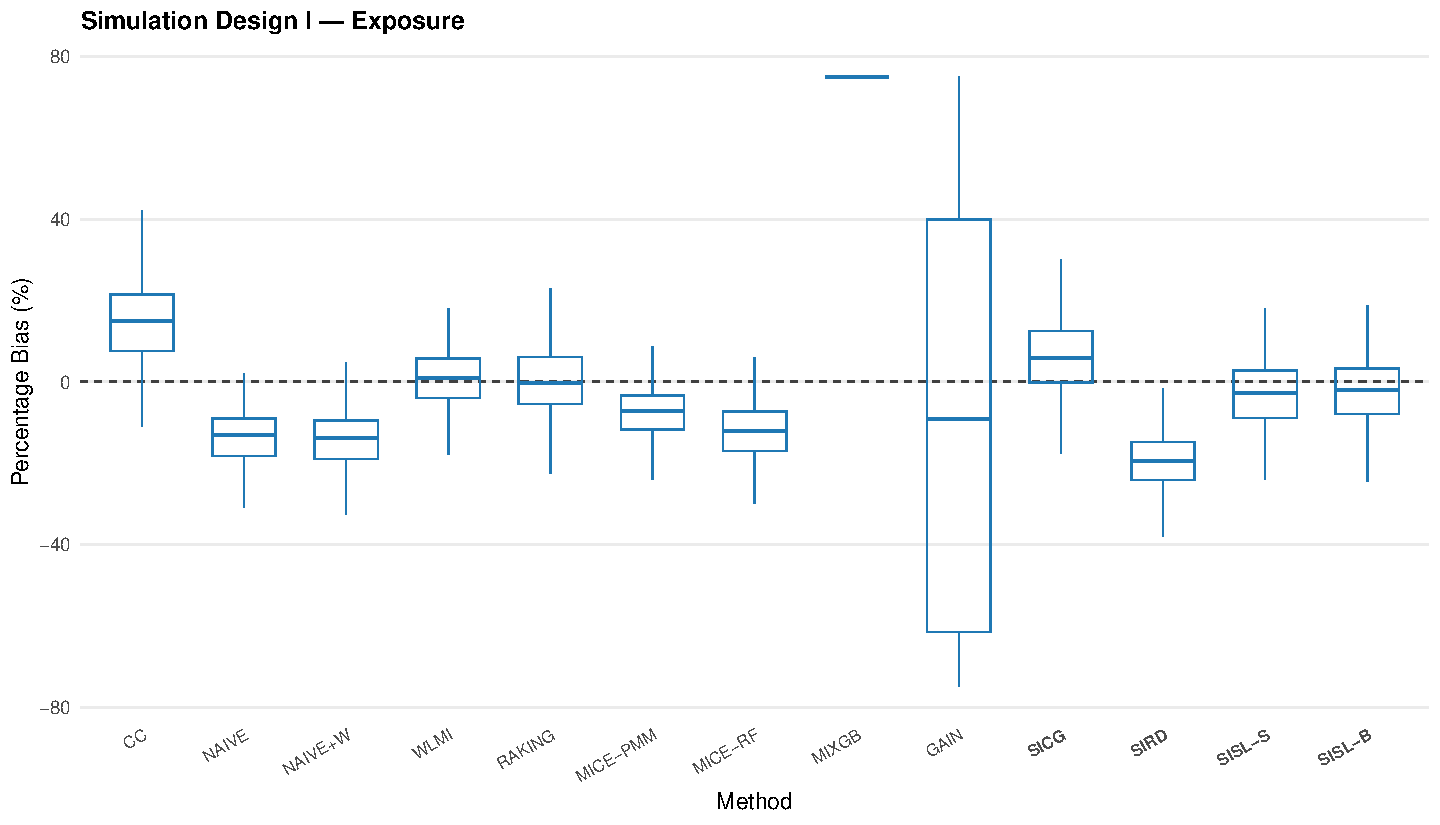
\includegraphics[width=\linewidth,height=0.86\textheight,keepaspectratio]{sisl_pctbias.pdf}
\caption{Per-replicate percentage bias of the exposure coefficient $\beta_X$ under Simulation Design~I, by imputation method, over 500 replicates. The dashed line marks zero bias; the proposed methods SICG, SIRD, SISL-S (sandwich variance) and SISL-B (bootstrap variance) are shown in bold. Extreme methods are clipped to $\pm100\%$ for legibility. TabCSDI, run on $100$ of the $500$ replicates, is not shown in this per-replicate figure; its summary appears in the benchmark table above.}
\label{fig:sisl_pctbias}
\end{figure}

\begin{figure}[p]
\centering
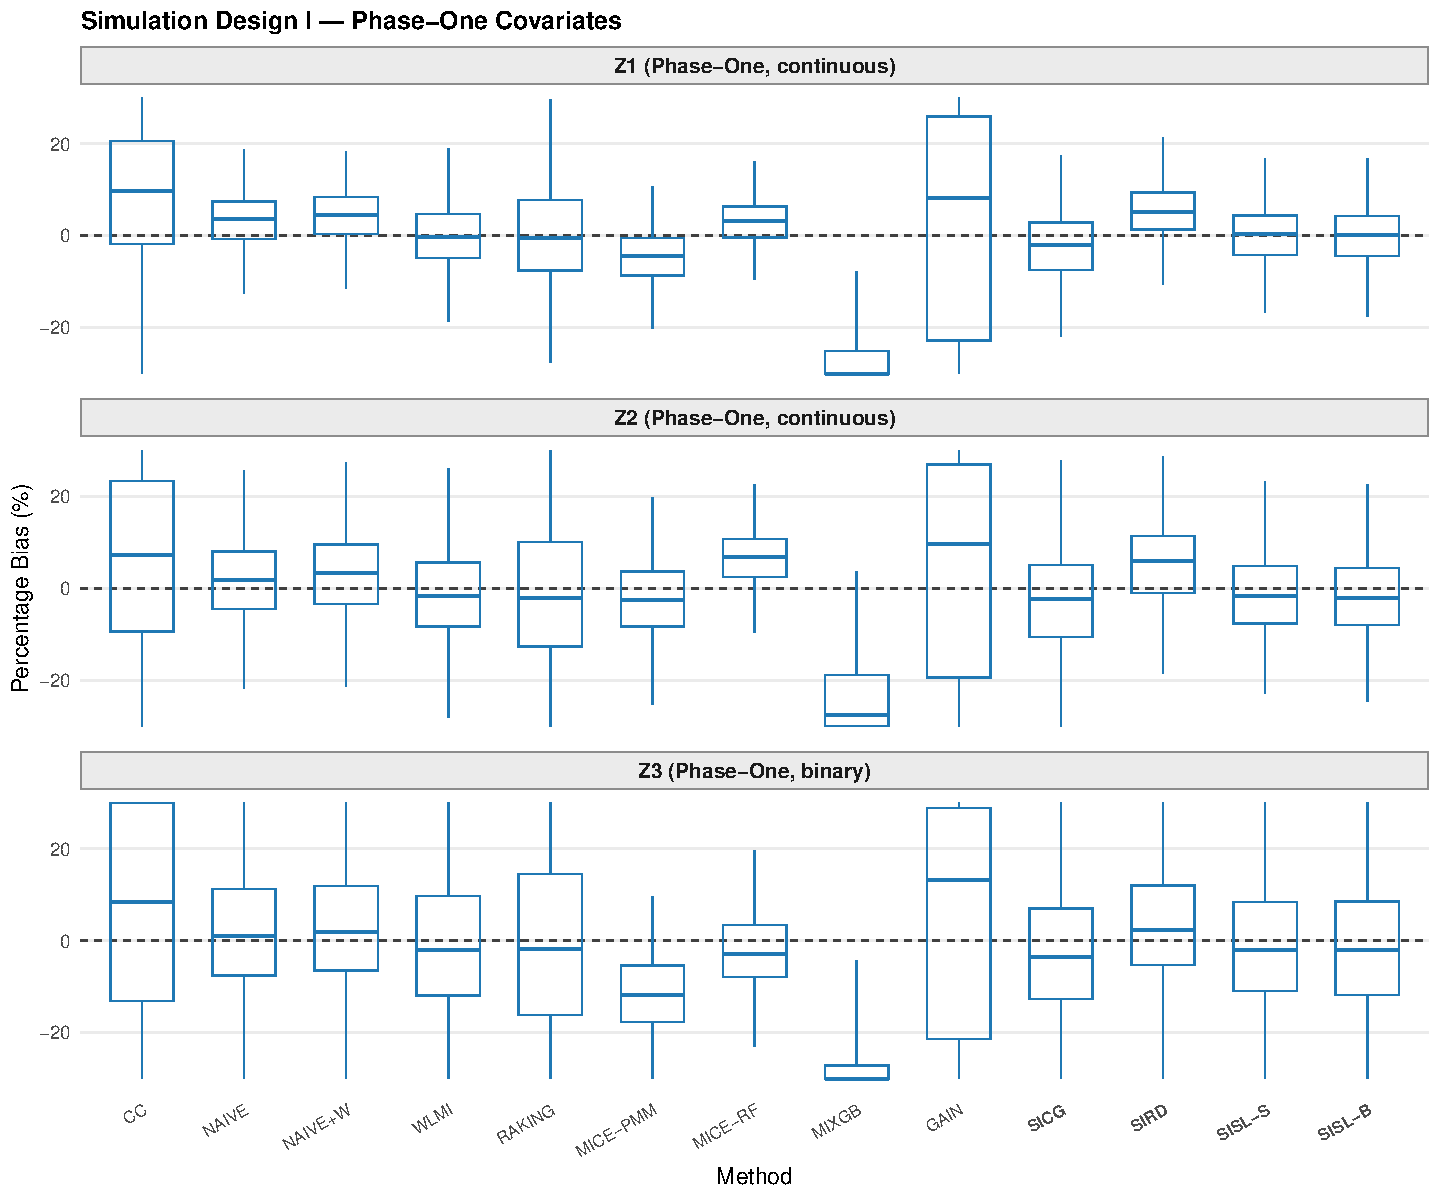
\includegraphics[width=\linewidth,height=0.86\textheight,keepaspectratio]{sisl_phase1cov_pctbias.pdf}
\caption{Per-replicate percentage bias of the fully observed Phase-One covariates ($Z_1$, $Z_2$ continuous; $Z_3$ binary) under Simulation Design~I, by imputation method, over 500 replicates. The dashed line marks zero bias; the proposed methods SICG, SIRD, SISL-S (sandwich variance) and SISL-B (bootstrap variance) are shown in bold. Extreme methods are clipped for legibility. TabCSDI, run on $100$ of the $500$ replicates, is not shown in this per-replicate figure; its summary appears in the benchmark table above.}
\label{fig:sisl_phase1cov}
\end{figure}

\clearpage
\section{Simulation Design~II}
\label{app:suppC_simI}

This section collects the full supplementary results for Simulation Design~II, the generalised-linear-model design of Chapter~\ref{chap:SICG}. Results are reported for the Gaussian and the Binomial analysis models in turn, by coefficient group, separating the imputed Phase-Two exposure from the fully observed Phase-One covariates; the full per-design metric tables appear first, followed by the per-replicate percentage-bias figures.

\subsection{Full per-design metrics}

\begin{landscape}
\definecolor{rankone}{RGB}{33,113,181}\definecolor{ranktwo}{RGB}{107,174,214}\definecolor{rankthree}{RGB}{198,219,239}
\footnotesize\setlength{\tabcolsep}{3.5pt}
\begin{longtable}{llrrrrrrrrrr}
\caption{Full simulation metrics for the Gaussian model of Simulation Design~II over all sampling designs. Metrics are averaged within coefficient groups. Mean $|$bias$|$ and relative RMSE use the log scale, which reduces the influence of extreme relative errors when a true coefficient is close to zero, although relative metrics still require caution near the null. Coverages use arithmetic means. Error metrics are ranked ascending, SE ratios by proximity to one, and coverages by proximity to $0.95$. The three best distinct ranks per row are shaded; displayed ties receive the same shade.}
\label{tab:appc_nutri_Gaussian} \\
\toprule
Design & Metric & \multicolumn{1}{c}{CC} & \multicolumn{1}{c}{UNVAL} & \multicolumn{1}{c}{MICE-PMM} & \multicolumn{1}{c}{MICE-RF} & \multicolumn{1}{c}{MIXGB} & \multicolumn{1}{c}{TabCSDI} & \multicolumn{1}{c}{GAIN} & \multicolumn{1}{c}{RAKING} & \multicolumn{1}{c}{\textbf{SICG}} & \multicolumn{1}{c}{\textbf{SIRD}} \\
\midrule
\endfirsthead
\multicolumn{12}{l}{\footnotesize\itshape Table~\ref{tab:appc_nutri_Gaussian} (continued)} \\
\toprule
Design & Metric & \multicolumn{1}{c}{CC} & \multicolumn{1}{c}{UNVAL} & \multicolumn{1}{c}{MICE-PMM} & \multicolumn{1}{c}{MICE-RF} & \multicolumn{1}{c}{MIXGB} & \multicolumn{1}{c}{TabCSDI} & \multicolumn{1}{c}{GAIN} & \multicolumn{1}{c}{RAKING} & \multicolumn{1}{c}{\textbf{SICG}} & \multicolumn{1}{c}{\textbf{SIRD}} \\
\midrule
\endhead
\midrule \multicolumn{12}{r}{\footnotesize\itshape continued on next page} \\
\endfoot
\bottomrule
\endlastfoot
\multicolumn{12}{l}{\textbf{Continuous Phase-Two Covariates}} \\
\addlinespace[2pt]
\quad \texttt{SRS} & Mean $|$Bias$|$ (\%) & \cellcolor{rankone}0.1 & 62.8 & 26.7 & 37.1 & 88.6 & 17.6 & 44.1 & \cellcolor{ranktwo}0.2 & 4.7 & \cellcolor{rankthree}3.1 \\
 & Rel.\ RMSE (\%) & \cellcolor{ranktwo}5.0 & 62.8 & 28.4 & 37.2 & 89.0 & 20.5 & 69.2 & \cellcolor{rankone}4.6 & 6.1 & \cellcolor{rankthree}5.5 \\
 & Emp.\ SE & 1.374 & 0.321 & 2.642 & 0.746 & 2.183 & 2.905 & 14.670 & 1.273 & 1.072 & 1.260 \\
 & Mean SE & 1.385 & 0.323 & 0.621 & 0.774 & 0.858 & 0.510 & 0.405 & 1.269 & 0.429 & 1.395 \\
 & SE ratio & \cellcolor{ranktwo}1.01 & \cellcolor{ranktwo}1.01 & 0.24 & \cellcolor{rankthree}1.04 & 0.39 & 0.18 & 0.03 & \cellcolor{rankone}1.00 & 0.40 & 1.11 \\
 & Nom.\ Cov. & \cellcolor{rankone}0.95 & 0.00 & 0.00 & 0.00 & 0.00 & 0.05 & 0.02 & \cellcolor{rankone}0.95 & \cellcolor{rankthree}0.32 & \cellcolor{ranktwo}0.94 \\
 & Orc.\ Cov.\ (Emp) & \cellcolor{rankone}0.95 & 0.00 & 0.26 & 0.00 & 0.00 & 0.67 & \cellcolor{rankone}0.95 & \cellcolor{rankone}0.95 & \cellcolor{rankthree}0.76 & \cellcolor{ranktwo}0.89 \\
 & Orc.\ Cov.\ (BC) & \cellcolor{rankone}0.95 & \cellcolor{rankone}0.95 & 0.22 & \cellcolor{rankone}0.95 & \cellcolor{rankthree}0.55 & 0.26 & 0.04 & \cellcolor{rankone}0.95 & \cellcolor{ranktwo}0.56 & \cellcolor{rankone}0.95 \\
\addlinespace[2pt]
\quad \texttt{RS} & Mean $|$Bias$|$ (\%) & 92.3 & 62.8 & 30.5 & 48.1 & 87.1 & \cellcolor{rankone}5.3 & 41.1 & 64.7 & \cellcolor{rankthree}18.8 & \cellcolor{ranktwo}7.6 \\
 & Rel.\ RMSE (\%) & 92.3 & 62.8 & 31.1 & 48.6 & 87.9 & \cellcolor{rankone}8.2 & 58.7 & 65.9 & \cellcolor{rankthree}19.4 & \cellcolor{ranktwo}8.8 \\
 & Emp.\ SE & 1.010 & 0.321 & 1.660 & 1.956 & 3.272 & 1.742 & 11.519 & 3.430 & 1.307 & 1.240 \\
 & Mean SE & 1.325 & 0.323 & 0.875 & 0.633 & 2.585 & 0.344 & 0.337 & 2.126 & 0.351 & 1.483 \\
 & SE ratio & 1.31 & \cellcolor{rankone}1.01 & 0.53 & 0.32 & \cellcolor{rankthree}0.79 & 0.20 & 0.03 & 0.62 & 0.27 & \cellcolor{ranktwo}1.20 \\
 & Nom.\ Cov. & 0.00 & 0.00 & 0.00 & 0.00 & 0.00 & \cellcolor{ranktwo}0.26 & \cellcolor{rankthree}0.02 & 0.00 & 0.00 & \cellcolor{rankone}0.80 \\
 & Orc.\ Cov.\ (Emp) & 0.00 & 0.00 & 0.00 & 0.00 & 0.00 & \cellcolor{rankone}0.89 & \cellcolor{rankone}0.89 & 0.00 & \cellcolor{rankthree}0.02 & \cellcolor{ranktwo}0.61 \\
 & Orc.\ Cov.\ (BC) & \cellcolor{rankthree}0.99 & \cellcolor{rankone}0.95 & 0.72 & 0.51 & 0.85 & 0.27 & 0.04 & 0.79 & 0.35 & \cellcolor{ranktwo}0.97 \\
\addlinespace[2pt]
\quad \texttt{WRS} & Mean $|$Bias$|$ (\%) & 82.3 & 62.8 & 49.9 & 35.0 & 39.1 & \cellcolor{rankone}0.2 & 36.6 & 64.0 & \cellcolor{rankthree}9.6 & \cellcolor{ranktwo}1.3 \\
 & Rel.\ RMSE (\%) & 82.4 & 62.8 & 50.0 & 35.1 & 39.9 & \cellcolor{ranktwo}6.2 & 54.6 & 64.3 & \cellcolor{rankthree}10.9 & \cellcolor{rankone}4.8 \\
 & Emp.\ SE & 0.945 & 0.321 & 0.612 & 0.553 & 2.128 & 1.713 & 11.130 & 1.675 & 1.419 & 1.269 \\
 & Mean SE & 1.105 & 0.323 & 0.497 & 0.548 & 1.798 & 0.331 & 0.330 & 1.169 & 0.337 & 1.569 \\
 & SE ratio & \cellcolor{rankthree}1.17 & \cellcolor{rankone}1.01 & 0.81 & \cellcolor{rankone}0.99 & \cellcolor{ranktwo}0.84 & 0.19 & 0.03 & 0.70 & 0.24 & 1.24 \\
 & Nom.\ Cov. & 0.00 & 0.00 & 0.00 & 0.00 & 0.00 & \cellcolor{ranktwo}0.29 & 0.02 & 0.00 & \cellcolor{rankthree}0.06 & \cellcolor{rankone}0.98 \\
 & Orc.\ Cov.\ (Emp) & 0.00 & 0.00 & 0.00 & 0.00 & 0.00 & \cellcolor{rankone}0.96 & \cellcolor{ranktwo}0.89 & 0.00 & \cellcolor{rankthree}0.56 & \cellcolor{rankone}0.94 \\
 & Orc.\ Cov.\ (BC) & \cellcolor{rankthree}0.98 & \cellcolor{rankone}0.95 & 0.88 & \cellcolor{ranktwo}0.94 & 0.89 & 0.30 & 0.05 & 0.82 & 0.36 & \cellcolor{rankthree}0.98 \\
\addlinespace[2pt]
\quad \texttt{SFS} & Mean $|$Bias$|$ (\%) & 84.5 & 62.8 & 48.5 & 43.7 & 76.9 & \cellcolor{rankone}0.4 & \cellcolor{rankthree}39.0 & 63.8 & \cellcolor{ranktwo}8.2 & \cellcolor{rankone}0.4 \\
 & Rel.\ RMSE (\%) & 84.6 & 62.8 & 48.6 & 43.9 & 77.7 & \cellcolor{ranktwo}7.5 & 56.6 & 64.2 & \cellcolor{rankthree}9.6 & \cellcolor{rankone}4.6 \\
 & Emp.\ SE & 0.911 & 0.321 & 0.703 & 1.073 & 3.101 & 2.065 & 11.258 & 1.911 & 1.392 & 1.272 \\
 & Mean SE & 1.093 & 0.323 & 0.490 & 0.572 & 3.121 & 0.326 & 0.330 & 1.305 & 0.344 & 1.654 \\
 & SE ratio & \cellcolor{ranktwo}1.20 & \cellcolor{rankone}1.01 & \cellcolor{rankthree}0.70 & 0.53 & \cellcolor{rankone}1.01 & 0.16 & 0.03 & 0.68 & 0.25 & \cellcolor{rankthree}1.30 \\
 & Nom.\ Cov. & 0.00 & 0.00 & 0.00 & 0.00 & 0.00 & \cellcolor{ranktwo}0.28 & 0.03 & 0.00 & \cellcolor{rankthree}0.12 & \cellcolor{rankone}0.98 \\
 & Orc.\ Cov.\ (Emp) & 0.00 & 0.00 & 0.00 & 0.00 & 0.00 & \cellcolor{ranktwo}0.93 & \cellcolor{rankthree}0.89 & 0.00 & 0.63 & \cellcolor{rankone}0.95 \\
 & Orc.\ Cov.\ (BC) & \cellcolor{rankthree}0.97 & \cellcolor{rankone}0.95 & 0.84 & 0.68 & \cellcolor{ranktwo}0.94 & 0.27 & 0.03 & 0.82 & 0.37 & 0.98 \\
\addlinespace[2pt]
\quad \texttt{ODS-Tail} & Mean $|$Bias$|$ (\%) & 40.3 & 62.8 & 63.3 & 54.7 & \cellcolor{ranktwo}17.0 & 32.5 & 27.1 & 30.4 & \cellcolor{rankthree}19.3 & \cellcolor{rankone}5.2 \\
 & Rel.\ RMSE (\%) & 40.7 & 62.8 & 63.3 & 54.8 & \cellcolor{ranktwo}18.7 & 33.0 & 52.1 & 31.3 & \cellcolor{rankthree}19.9 & \cellcolor{rankone}7.0 \\
 & Emp.\ SE & 1.606 & 0.321 & 0.382 & 1.057 & 2.171 & 1.575 & 12.243 & 2.033 & 1.343 & 1.313 \\
 & Mean SE & 1.358 & 0.323 & 0.312 & 0.641 & 2.520 & 0.316 & 0.351 & 1.694 & 0.417 & 1.591 \\
 & SE ratio & \cellcolor{ranktwo}0.85 & \cellcolor{rankone}1.01 & 0.82 & 0.61 & \cellcolor{rankthree}1.16 & 0.20 & 0.03 & 0.83 & 0.31 & 1.21 \\
 & Nom.\ Cov. & 0.00 & 0.00 & 0.00 & 0.00 & \cellcolor{ranktwo}0.62 & 0.00 & \cellcolor{rankthree}0.02 & 0.01 & 0.00 & \cellcolor{rankone}0.89 \\
 & Orc.\ Cov.\ (Emp) & 0.00 & 0.00 & 0.00 & 0.00 & \cellcolor{rankthree}0.45 & 0.00 & \cellcolor{rankone}0.98 & 0.02 & 0.03 & \cellcolor{ranktwo}0.81 \\
 & Orc.\ Cov.\ (BC) & 0.90 & \cellcolor{rankone}0.95 & 0.89 & 0.82 & \cellcolor{ranktwo}0.96 & 0.33 & 0.01 & 0.89 & 0.47 & \cellcolor{rankthree}0.98 \\
\addlinespace[2pt]
\quad \texttt{Neyman-ODS} & Mean $|$Bias$|$ (\%) & \cellcolor{ranktwo}0.4 & 62.8 & 38.6 & 24.6 & 87.7 & 8.5 & 45.9 & \cellcolor{rankone}0.1 & 8.3 & \cellcolor{rankthree}2.6 \\
 & Rel.\ RMSE (\%) & \cellcolor{ranktwo}5.0 & 62.8 & 42.0 & 25.0 & 88.0 & 10.6 & 61.1 & \cellcolor{rankone}4.8 & 9.3 & \cellcolor{rankthree}5.3 \\
 & Emp.\ SE & 1.364 & 0.321 & 4.563 & 1.204 & 2.147 & 1.727 & 11.092 & 1.313 & 1.178 & 1.258 \\
 & Mean SE & 1.389 & 0.323 & 0.879 & 0.631 & 0.810 & 0.459 & 0.368 & 1.236 & 0.409 & 1.363 \\
 & SE ratio & \cellcolor{ranktwo}1.02 & \cellcolor{rankone}1.01 & 0.19 & 0.52 & 0.38 & 0.27 & 0.03 & \cellcolor{rankthree}0.94 & 0.35 & 1.08 \\
 & Nom.\ Cov. & \cellcolor{rankone}0.95 & 0.00 & 0.00 & 0.00 & 0.00 & 0.18 & 0.02 & \cellcolor{rankthree}0.93 & 0.09 & \cellcolor{ranktwo}0.94 \\
 & Orc.\ Cov.\ (Emp) & \cellcolor{rankone}0.96 & 0.00 & 0.43 & 0.00 & 0.00 & 0.71 & \cellcolor{rankthree}0.80 & \cellcolor{rankone}0.94 & 0.48 & \cellcolor{ranktwo}0.91 \\
 & Orc.\ Cov.\ (BC) & \cellcolor{ranktwo}0.96 & \cellcolor{rankone}0.95 & 0.16 & 0.68 & 0.55 & 0.39 & 0.06 & \cellcolor{rankthree}0.93 & 0.47 & \cellcolor{ranktwo}0.96 \\
\addlinespace[2pt]
\quad \texttt{Neyman-IF} & Mean $|$Bias$|$ (\%) & 10.1 & 62.8 & 26.4 & 24.7 & 86.6 & 10.8 & 49.4 & \cellcolor{rankone}0.2 & \cellcolor{rankthree}8.4 & \cellcolor{ranktwo}1.6 \\
 & Rel.\ RMSE (\%) & 11.3 & 62.8 & 27.5 & 25.0 & 86.9 & 12.9 & 61.9 & \cellcolor{rankone}5.0 & \cellcolor{rankthree}9.6 & \cellcolor{ranktwo}5.1 \\
 & Emp.\ SE & 1.419 & 0.321 & 2.042 & 1.186 & 2.058 & 1.966 & 10.266 & 1.381 & 1.255 & 1.344 \\
 & Mean SE & 1.396 & 0.323 & 0.824 & 0.637 & 0.774 & 0.463 & 0.355 & 1.223 & 0.413 & 1.392 \\
 & SE ratio & \cellcolor{ranktwo}0.98 & \cellcolor{rankone}1.01 & 0.40 & 0.54 & 0.38 & 0.24 & 0.03 & 0.89 & 0.33 & \cellcolor{rankthree}1.04 \\
 & Nom.\ Cov. & \cellcolor{rankthree}0.47 & 0.00 & 0.01 & 0.00 & 0.00 & 0.13 & 0.02 & \cellcolor{ranktwo}0.91 & 0.10 & \cellcolor{rankone}0.95 \\
 & Orc.\ Cov.\ (Emp) & 0.50 & 0.00 & 0.06 & 0.00 & 0.00 & \cellcolor{ranktwo}0.72 & \cellcolor{rankthree}0.71 & \cellcolor{rankone}0.94 & 0.56 & \cellcolor{rankone}0.94 \\
 & Orc.\ Cov.\ (BC) & \cellcolor{rankone}0.95 & \cellcolor{rankone}0.95 & 0.59 & 0.71 & 0.53 & 0.43 & 0.06 & \cellcolor{rankthree}0.92 & 0.48 & \cellcolor{ranktwo}0.96 \\
\addlinespace[2pt]
\multicolumn{12}{l}{\textbf{Continuous Phase-One Covariates}} \\
\addlinespace[2pt]
\quad \texttt{SRS} & Mean $|$Bias$|$ (\%) & \cellcolor{ranktwo}24.5 & 181.6 & 70.8 & 176.1 & 161.5 & 189.7 & 46.7 & \cellcolor{rankone}22.2 & \cellcolor{rankthree}33.3 & 67.0 \\
 & Rel.\ RMSE (\%) & 136.2 & 189.1 & 155.6 & 181.4 & 205.7 & 196.3 & 211.0 & \cellcolor{rankthree}127.9 & \cellcolor{rankone}87.6 & \cellcolor{ranktwo}103.0 \\
 & Emp.\ SE & 0.464 & 0.106 & 0.262 & 0.127 & 0.461 & 0.167 & 0.591 & 0.423 & 0.273 & 0.275 \\
 & Mean SE & 0.472 & 0.105 & 0.195 & 0.176 & 0.218 & 0.166 & 0.120 & 0.421 & 0.140 & 0.295 \\
 & SE ratio & \cellcolor{rankthree}1.02 & \cellcolor{ranktwo}0.99 & 0.74 & 1.39 & 0.47 & \cellcolor{ranktwo}0.99 & 0.20 & \cellcolor{rankone}1.00 & 0.51 & 1.07 \\
 & Nom.\ Cov. & \cellcolor{rankone}0.83 & 0.16 & 0.44 & 0.24 & 0.27 & 0.05 & 0.24 & \cellcolor{ranktwo}0.81 & \cellcolor{rankthree}0.46 & \cellcolor{ranktwo}0.81 \\
 & Orc.\ Cov.\ (Emp) & \cellcolor{rankthree}0.82 & 0.16 & 0.49 & 0.08 & 0.51 & 0.03 & \cellcolor{rankone}0.96 & \cellcolor{rankthree}0.82 & \cellcolor{ranktwo}0.83 & 0.76 \\
 & Orc.\ Cov.\ (BC) & \cellcolor{ranktwo}0.96 & \cellcolor{ranktwo}0.96 & 0.77 & \cellcolor{rankthree}0.97 & 0.64 & 0.75 & 0.24 & \cellcolor{rankone}0.95 & 0.63 & \cellcolor{ranktwo}0.94 \\
\addlinespace[2pt]
\quad \texttt{RS} & Mean $|$Bias$|$ (\%) & 167.9 & 181.6 & 140.9 & 171.6 & \cellcolor{ranktwo}34.3 & 141.9 & \cellcolor{rankthree}42.6 & 145.4 & 85.2 & \cellcolor{rankone}21.7 \\
 & Rel.\ RMSE (\%) & 231.0 & 189.1 & 156.9 & 177.0 & \cellcolor{rankthree}139.6 & 152.4 & 187.8 & 329.9 & \cellcolor{ranktwo}115.7 & \cellcolor{rankone}104.9 \\
 & Emp.\ SE & 0.387 & 0.106 & 0.224 & 0.118 & 0.418 & 0.149 & 0.510 & 0.975 & 0.305 & 0.273 \\
 & Mean SE & 0.483 & 0.105 & 0.191 & 0.128 & 0.365 & 0.116 & 0.102 & 0.718 & 0.116 & 0.309 \\
 & SE ratio & 1.25 & \cellcolor{rankone}0.99 & 0.85 & \cellcolor{ranktwo}1.08 & \cellcolor{rankthree}0.87 & 0.78 & 0.20 & 0.74 & 0.38 & \cellcolor{rankthree}1.13 \\
 & Nom.\ Cov. & 0.52 & 0.16 & 0.32 & 0.13 & \cellcolor{ranktwo}0.74 & 0.04 & 0.26 & \cellcolor{rankthree}0.72 & 0.31 & \cellcolor{rankone}0.82 \\
 & Orc.\ Cov.\ (Emp) & 0.48 & 0.16 & 0.36 & 0.08 & \cellcolor{rankthree}0.81 & 0.23 & \cellcolor{rankone}0.95 & \cellcolor{ranktwo}0.87 & 0.79 & 0.75 \\
 & Orc.\ Cov.\ (BC) & \cellcolor{ranktwo}0.97 & \cellcolor{rankone}0.96 & \cellcolor{rankthree}0.91 & 0.89 & 0.88 & 0.66 & 0.27 & 0.84 & 0.51 & \cellcolor{rankone}0.96 \\
\addlinespace[2pt]
\quad \texttt{WRS} & Mean $|$Bias$|$ (\%) & 169.6 & 181.6 & 167.4 & 154.5 & \cellcolor{ranktwo}41.4 & 141.3 & \cellcolor{rankone}39.8 & 160.0 & \cellcolor{rankthree}57.8 & 64.6 \\
 & Rel.\ RMSE (\%) & 218.2 & 189.1 & 173.2 & 158.6 & \cellcolor{rankone}86.1 & 150.7 & 190.5 & 222.0 & \cellcolor{ranktwo}96.3 & \cellcolor{rankthree}112.4 \\
 & Emp.\ SE & 0.366 & 0.106 & 0.106 & 0.094 & 0.270 & 0.145 & 0.502 & 0.473 & 0.284 & 0.272 \\
 & Mean SE & 0.411 & 0.105 & 0.128 & 0.121 & 0.191 & 0.111 & 0.100 & 0.422 & 0.112 & 0.318 \\
 & SE ratio & \cellcolor{rankthree}1.12 & \cellcolor{rankone}0.99 & 1.21 & 1.29 & 0.71 & 0.77 & 0.20 & \cellcolor{ranktwo}0.89 & 0.39 & 1.17 \\
 & Nom.\ Cov. & 0.52 & 0.16 & 0.20 & 0.17 & \cellcolor{ranktwo}0.73 & 0.04 & 0.26 & \cellcolor{rankthree}0.60 & 0.37 & \cellcolor{rankone}0.81 \\
 & Orc.\ Cov.\ (Emp) & 0.50 & 0.16 & 0.11 & 0.06 & \cellcolor{ranktwo}0.91 & 0.22 & \cellcolor{rankone}0.95 & 0.65 & \cellcolor{rankthree}0.87 & 0.74 \\
 & Orc.\ Cov.\ (BC) & \cellcolor{rankone}0.96 & \cellcolor{rankone}0.96 & \cellcolor{ranktwo}0.97 & \cellcolor{ranktwo}0.97 & \cellcolor{rankthree}0.81 & 0.68 & 0.28 & \cellcolor{ranktwo}0.93 & 0.51 & \cellcolor{rankone}0.96 \\
\addlinespace[2pt]
\quad \texttt{SFS} & Mean $|$Bias$|$ (\%) & 167.2 & 181.6 & 144.8 & 141.9 & \cellcolor{rankthree}70.2 & 141.1 & \cellcolor{rankone}37.5 & 141.5 & \cellcolor{ranktwo}52.7 & 73.2 \\
 & Rel.\ RMSE (\%) & 217.2 & 189.1 & 154.3 & 148.2 & \cellcolor{rankthree}135.6 & 150.2 & 194.7 & 234.1 & \cellcolor{rankone}92.9 & \cellcolor{ranktwo}114.7 \\
 & Emp.\ SE & 0.356 & 0.106 & 0.113 & 0.103 & 0.381 & 0.156 & 0.531 & 0.562 & 0.294 & 0.285 \\
 & Mean SE & 0.414 & 0.105 & 0.128 & 0.118 & 0.335 & 0.111 & 0.100 & 0.486 & 0.114 & 0.317 \\
 & SE ratio & 1.16 & \cellcolor{rankone}0.99 & 1.13 & 1.15 & \cellcolor{rankthree}0.88 & 0.71 & 0.19 & 0.86 & 0.39 & \cellcolor{ranktwo}1.11 \\
 & Nom.\ Cov. & 0.53 & 0.16 & 0.31 & 0.25 & \cellcolor{ranktwo}0.75 & 0.04 & 0.27 & \cellcolor{rankthree}0.65 & 0.42 & \cellcolor{rankone}0.82 \\
 & Orc.\ Cov.\ (Emp) & 0.49 & 0.16 & 0.27 & 0.17 & \cellcolor{rankthree}0.83 & 0.22 & \cellcolor{rankone}0.95 & 0.68 & \cellcolor{ranktwo}0.89 & 0.74 \\
 & Orc.\ Cov.\ (BC) & \cellcolor{ranktwo}0.96 & \cellcolor{ranktwo}0.96 & \cellcolor{ranktwo}0.96 & \cellcolor{rankthree}0.97 & 0.88 & 0.65 & 0.27 & \cellcolor{rankthree}0.93 & 0.51 & \cellcolor{rankone}0.95 \\
\addlinespace[2pt]
\quad \texttt{ODS-Tail} & Mean $|$Bias$|$ (\%) & 103.8 & 181.6 & 133.9 & 146.9 & 106.9 & 123.3 & \cellcolor{rankone}34.7 & 95.5 & \cellcolor{rankthree}71.8 & \cellcolor{ranktwo}65.6 \\
 & Rel.\ RMSE (\%) & 141.6 & 189.1 & 140.0 & 150.3 & 131.6 & \cellcolor{rankthree}130.6 & 246.1 & 151.8 & \cellcolor{rankone}101.7 & \cellcolor{ranktwo}110.0 \\
 & Emp.\ SE & 0.340 & 0.106 & 0.096 & 0.092 & 0.285 & 0.124 & 0.789 & 0.440 & 0.215 & 0.245 \\
 & Mean SE & 0.361 & 0.105 & 0.119 & 0.119 & 0.336 & 0.103 & 0.104 & 0.413 & 0.121 & 0.313 \\
 & SE ratio & \cellcolor{ranktwo}1.06 & \cellcolor{rankone}0.99 & 1.24 & 1.29 & 1.18 & \cellcolor{rankthree}0.83 & 0.13 & \cellcolor{ranktwo}0.94 & 0.56 & 1.28 \\
 & Nom.\ Cov. & \cellcolor{ranktwo}0.84 & 0.16 & 0.29 & 0.11 & 0.66 & 0.05 & 0.14 & \cellcolor{rankone}0.85 & 0.31 & \cellcolor{rankthree}0.81 \\
 & Orc.\ Cov.\ (Emp) & \cellcolor{rankthree}0.81 & 0.16 & 0.16 & 0.03 & 0.62 & 0.20 & \cellcolor{rankone}0.95 & \cellcolor{ranktwo}0.86 & 0.66 & 0.66 \\
 & Orc.\ Cov.\ (BC) & \cellcolor{rankone}0.96 & \cellcolor{rankone}0.96 & \cellcolor{ranktwo}0.97 & \cellcolor{rankone}0.94 & \cellcolor{rankone}0.94 & \cellcolor{rankthree}0.76 & 0.15 & \cellcolor{rankone}0.94 & 0.67 & \cellcolor{ranktwo}0.97 \\
\addlinespace[2pt]
\quad \texttt{Neyman-ODS} & Mean $|$Bias$|$ (\%) & \cellcolor{rankone}10.0 & 181.6 & 175.5 & 183.0 & 166.2 & 199.3 & 59.7 & \cellcolor{rankthree}19.8 & \cellcolor{ranktwo}17.3 & 67.0 \\
 & Rel.\ RMSE (\%) & 141.4 & 189.1 & 203.3 & 187.8 & 203.6 & 204.7 & 206.8 & \cellcolor{rankthree}128.2 & \cellcolor{rankone}92.5 & \cellcolor{ranktwo}100.4 \\
 & Emp.\ SE & 0.476 & 0.106 & 0.277 & 0.145 & 0.437 & 0.164 & 0.617 & 0.440 & 0.281 & 0.256 \\
 & Mean SE & 0.474 & 0.105 & 0.210 & 0.163 & 0.210 & 0.151 & 0.113 & 0.425 & 0.135 & 0.287 \\
 & SE ratio & \cellcolor{rankone}1.00 & \cellcolor{ranktwo}0.99 & 0.76 & 1.12 & 0.48 & 0.92 & 0.18 & \cellcolor{rankthree}0.97 & 0.48 & 1.12 \\
 & Nom.\ Cov. & \cellcolor{rankone}0.82 & 0.16 & 0.32 & 0.09 & 0.24 & 0.02 & 0.18 & \cellcolor{rankthree}0.79 & 0.42 & \cellcolor{ranktwo}0.80 \\
 & Orc.\ Cov.\ (Emp) & \cellcolor{ranktwo}0.82 & 0.16 & 0.39 & 0.05 & 0.53 & 0.02 & \cellcolor{rankone}0.95 & \cellcolor{rankthree}0.80 & \cellcolor{ranktwo}0.82 & 0.72 \\
 & Orc.\ Cov.\ (BC) & \cellcolor{rankone}0.95 & \cellcolor{ranktwo}0.96 & 0.69 & \cellcolor{rankone}0.95 & 0.60 & \cellcolor{rankthree}0.84 & 0.20 & \cellcolor{rankone}0.95 & 0.60 & \cellcolor{ranktwo}0.96 \\
\addlinespace[2pt]
\quad \texttt{Neyman-IF} & Mean $|$Bias$|$ (\%) & 62.1 & 181.6 & \cellcolor{rankthree}36.0 & 179.1 & 156.2 & 199.0 & 55.9 & \cellcolor{rankone}24.7 & \cellcolor{ranktwo}29.0 & 62.2 \\
 & Rel.\ RMSE (\%) & 149.8 & 189.1 & \cellcolor{rankthree}124.1 & 184.4 & 199.2 & 203.9 & 208.9 & 133.2 & \cellcolor{rankone}93.3 & \cellcolor{ranktwo}101.8 \\
 & Emp.\ SE & 0.467 & 0.106 & 0.177 & 0.150 & 0.446 & 0.150 & 0.596 & 0.424 & 0.296 & 0.290 \\
 & Mean SE & 0.471 & 0.105 & 0.195 & 0.162 & 0.205 & 0.153 & 0.109 & 0.421 & 0.137 & 0.314 \\
 & SE ratio & \cellcolor{rankone}1.01 & \cellcolor{rankone}0.99 & 1.10 & \cellcolor{rankthree}1.08 & 0.46 & \cellcolor{ranktwo}1.02 & 0.18 & \cellcolor{rankone}0.99 & 0.46 & \cellcolor{rankthree}1.08 \\
 & Nom.\ Cov. & \cellcolor{rankone}0.82 & 0.16 & \cellcolor{rankthree}0.49 & 0.09 & 0.26 & 0.02 & 0.20 & \cellcolor{ranktwo}0.77 & 0.42 & \cellcolor{rankone}0.82 \\
 & Orc.\ Cov.\ (Emp) & \cellcolor{rankthree}0.82 & 0.16 & 0.47 & 0.07 & 0.54 & 0.02 & \cellcolor{rankone}0.95 & 0.78 & \cellcolor{ranktwo}0.85 & 0.79 \\
 & Orc.\ Cov.\ (BC) & \cellcolor{rankone}0.95 & \cellcolor{ranktwo}0.96 & \cellcolor{rankthree}0.93 & \cellcolor{ranktwo}0.94 & 0.63 & 0.85 & 0.22 & \cellcolor{rankone}0.95 & 0.56 & \cellcolor{rankone}0.95 \\
\addlinespace[2pt]
\multicolumn{12}{l}{\textbf{Binary \& Categorical Phase-One Covariates}} \\
\addlinespace[2pt]
\quad \texttt{SRS} & Mean $|$Bias$|$ (\%) & \cellcolor{rankone}1.6 & 54.8 & 60.0 & 54.3 & 36.9 & 42.7 & 9.8 & \cellcolor{rankthree}6.9 & \cellcolor{rankthree}6.9 & \cellcolor{ranktwo}5.0 \\
 & Rel.\ RMSE (\%) & 66.7 & 67.4 & 64.2 & 61.4 & 68.7 & \cellcolor{rankthree}52.3 & 232.8 & 61.8 & \cellcolor{ranktwo}48.1 & \cellcolor{rankone}46.4 \\
 & Emp.\ SE & 1.338 & 0.385 & 0.464 & 0.396 & 0.823 & 0.579 & 4.725 & 1.181 & 0.934 & 0.906 \\
 & Mean SE & 1.321 & 0.377 & 0.385 & 0.401 & 0.432 & 0.378 & 0.273 & 1.133 & 0.346 & 0.856 \\
 & SE ratio & \cellcolor{rankone}0.99 & \cellcolor{ranktwo}0.98 & 0.83 & \cellcolor{rankone}1.01 & 0.52 & 0.65 & 0.06 & \cellcolor{rankthree}0.96 & 0.37 & 0.94 \\
 & Nom.\ Cov. & \cellcolor{rankone}0.94 & 0.33 & 0.21 & 0.31 & 0.48 & 0.40 & 0.11 & \cellcolor{ranktwo}0.93 & \cellcolor{rankthree}0.52 & \cellcolor{ranktwo}0.93 \\
 & Orc.\ Cov.\ (Emp) & \cellcolor{rankone}0.95 & 0.33 & 0.24 & 0.30 & \cellcolor{rankthree}0.73 & 0.57 & \cellcolor{ranktwo}0.94 & \cellcolor{ranktwo}0.94 & \cellcolor{ranktwo}0.94 & \cellcolor{ranktwo}0.94 \\
 & Orc.\ Cov.\ (BC) & \cellcolor{ranktwo}0.94 & \cellcolor{ranktwo}0.94 & 0.88 & \cellcolor{rankone}0.95 & 0.73 & 0.82 & 0.10 & \cellcolor{ranktwo}0.94 & 0.53 & \cellcolor{rankthree}0.93 \\
\addlinespace[2pt]
\quad \texttt{RS} & Mean $|$Bias$|$ (\%) & 73.7 & 54.8 & 45.3 & 61.3 & 35.5 & 37.8 & \cellcolor{rankthree}19.8 & 71.3 & \cellcolor{ranktwo}10.9 & \cellcolor{rankone}3.5 \\
 & Rel.\ RMSE (\%) & 142.1 & 67.4 & \cellcolor{rankone}52.4 & 67.9 & 66.6 & \cellcolor{ranktwo}55.6 & 297.1 & 240.1 & 73.2 & \cellcolor{rankthree}57.2 \\
 & Emp.\ SE & 1.877 & 0.385 & 0.401 & 0.500 & 0.856 & 0.811 & 5.909 & 4.200 & 1.175 & 1.101 \\
 & Mean SE & 1.946 & 0.377 & 0.408 & 0.411 & 0.734 & 0.328 & 0.261 & 3.282 & 0.310 & 1.080 \\
 & SE ratio & \cellcolor{ranktwo}1.04 & \cellcolor{rankone}0.98 & \cellcolor{rankone}1.02 & 0.82 & \cellcolor{rankthree}0.86 & 0.40 & 0.04 & 0.78 & 0.26 & \cellcolor{rankone}0.98 \\
 & Nom.\ Cov. & \cellcolor{rankthree}0.74 & 0.33 & 0.33 & 0.27 & 0.60 & 0.35 & 0.10 & \cellcolor{ranktwo}0.80 & 0.32 & \cellcolor{rankone}0.94 \\
 & Orc.\ Cov.\ (Emp) & 0.72 & 0.33 & 0.33 & 0.27 & 0.70 & \cellcolor{rankthree}0.81 & \cellcolor{rankone}0.94 & \cellcolor{ranktwo}0.90 & \cellcolor{rankthree}0.81 & \cellcolor{rankone}0.94 \\
 & Orc.\ Cov.\ (BC) & \cellcolor{rankone}0.95 & \cellcolor{ranktwo}0.94 & \cellcolor{ranktwo}0.94 & 0.89 & \cellcolor{rankthree}0.90 & 0.66 & 0.09 & 0.88 & 0.40 & \cellcolor{ranktwo}0.94 \\
\addlinespace[2pt]
\quad \texttt{WRS} & Mean $|$Bias$|$ (\%) & 68.8 & 54.8 & 55.9 & 56.8 & \cellcolor{rankthree}23.1 & 37.1 & 24.5 & 73.1 & \cellcolor{ranktwo}10.0 & \cellcolor{rankone}8.5 \\
 & Rel.\ RMSE (\%) & 128.5 & 67.4 & 59.9 & 62.7 & \cellcolor{rankone}49.2 & \cellcolor{rankthree}55.1 & 289.3 & 143.7 & 66.7 & \cellcolor{ranktwo}53.3 \\
 & Emp.\ SE & 1.729 & 0.385 & 0.382 & 0.387 & 0.744 & 0.771 & 5.793 & 2.120 & 1.117 & 1.041 \\
 & Mean SE & 1.778 & 0.377 & 0.382 & 0.391 & 0.513 & 0.327 & 0.262 & 1.997 & 0.311 & 1.035 \\
 & SE ratio & 1.03 & \cellcolor{rankthree}0.98 & \cellcolor{rankone}1.00 & \cellcolor{ranktwo}1.01 & 0.69 & 0.42 & 0.05 & 0.94 & 0.28 & \cellcolor{ranktwo}0.99 \\
 & Nom.\ Cov. & \cellcolor{rankthree}0.74 & 0.33 & 0.26 & 0.28 & 0.59 & 0.37 & 0.09 & \cellcolor{ranktwo}0.75 & 0.34 & \cellcolor{rankone}0.95 \\
 & Orc.\ Cov.\ (Emp) & 0.73 & 0.33 & 0.23 & 0.28 & 0.77 & 0.74 & \cellcolor{ranktwo}0.94 & 0.78 & \cellcolor{rankthree}0.85 & \cellcolor{rankone}0.95 \\
 & Orc.\ Cov.\ (BC) & \cellcolor{ranktwo}0.96 & \cellcolor{ranktwo}0.94 & \cellcolor{rankone}0.95 & \cellcolor{rankone}0.95 & 0.81 & 0.67 & 0.10 & \cellcolor{rankthree}0.93 & 0.42 & \cellcolor{rankone}0.95 \\
\addlinespace[2pt]
\quad \texttt{SFS} & Mean $|$Bias$|$ (\%) & 69.0 & 54.8 & 55.3 & 58.5 & 33.8 & 39.2 & \cellcolor{rankthree}10.9 & 77.6 & \cellcolor{rankone}5.4 & \cellcolor{ranktwo}6.1 \\
 & Rel.\ RMSE (\%) & 129.5 & 67.4 & \cellcolor{rankthree}59.3 & 64.0 & 67.1 & \cellcolor{ranktwo}56.9 & 290.7 & 152.4 & 66.2 & \cellcolor{rankone}52.3 \\
 & Emp.\ SE & 1.731 & 0.385 & 0.387 & 0.407 & 0.880 & 0.822 & 5.829 & 2.235 & 1.089 & 1.016 \\
 & Mean SE & 1.785 & 0.377 & 0.381 & 0.412 & 0.741 & 0.324 & 0.260 & 2.154 & 0.315 & 1.014 \\
 & SE ratio & 1.03 & \cellcolor{rankthree}0.98 & \cellcolor{rankthree}0.98 & \cellcolor{ranktwo}1.01 & 0.84 & 0.39 & 0.04 & 0.96 & 0.29 & \cellcolor{rankone}1.00 \\
 & Nom.\ Cov. & \cellcolor{rankthree}0.74 & 0.33 & 0.26 & 0.28 & 0.59 & 0.35 & 0.09 & \cellcolor{ranktwo}0.76 & 0.34 & \cellcolor{rankone}0.95 \\
 & Orc.\ Cov.\ (Emp) & 0.73 & 0.33 & 0.24 & 0.27 & 0.71 & 0.75 & \cellcolor{rankone}0.95 & 0.77 & \cellcolor{rankthree}0.83 & \cellcolor{ranktwo}0.94 \\
 & Orc.\ Cov.\ (BC) & \cellcolor{rankone}0.95 & \cellcolor{ranktwo}0.94 & \cellcolor{ranktwo}0.94 & \cellcolor{rankone}0.95 & \cellcolor{rankthree}0.90 & 0.62 & 0.09 & \cellcolor{ranktwo}0.94 & 0.42 & \cellcolor{ranktwo}0.94 \\
\addlinespace[2pt]
\quad \texttt{ODS-Tail} & Mean $|$Bias$|$ (\%) & 23.9 & 54.8 & 88.6 & 47.4 & \cellcolor{rankthree}19.3 & 40.0 & \cellcolor{ranktwo}10.5 & 30.0 & 32.7 & \cellcolor{rankone}8.4 \\
 & Rel.\ RMSE (\%) & 123.9 & 67.4 & 93.5 & \cellcolor{rankone}54.1 & \cellcolor{ranktwo}54.2 & 60.0 & 279.9 & 131.3 & 73.0 & \cellcolor{rankthree}55.0 \\
 & Emp.\ SE & 1.803 & 0.385 & 0.466 & 0.484 & 0.781 & 0.763 & 5.658 & 1.962 & 0.983 & 1.008 \\
 & Mean SE & 1.684 & 0.377 & 0.433 & 0.423 & 0.808 & 0.361 & 0.279 & 1.869 & 0.371 & 1.017 \\
 & SE ratio & 0.93 & \cellcolor{ranktwo}0.98 & 0.93 & 0.87 & \cellcolor{rankthree}1.03 & 0.47 & 0.05 & 0.95 & 0.38 & \cellcolor{rankone}1.01 \\
 & Nom.\ Cov. & \cellcolor{ranktwo}0.76 & 0.33 & 0.16 & 0.36 & 0.70 & 0.36 & 0.12 & \cellcolor{rankthree}0.75 & 0.40 & \cellcolor{rankone}0.93 \\
 & Orc.\ Cov.\ (Emp) & \cellcolor{rankthree}0.76 & 0.33 & 0.20 & 0.39 & 0.74 & 0.66 & \cellcolor{rankone}0.94 & \cellcolor{rankthree}0.76 & 0.73 & \cellcolor{ranktwo}0.92 \\
 & Orc.\ Cov.\ (BC) & \cellcolor{ranktwo}0.94 & \cellcolor{ranktwo}0.94 & \cellcolor{rankone}0.95 & 0.91 & \cellcolor{rankthree}0.93 & 0.72 & 0.11 & \cellcolor{ranktwo}0.94 & 0.54 & \cellcolor{ranktwo}0.94 \\
\addlinespace[2pt]
\quad \texttt{Neyman-ODS} & Mean $|$Bias$|$ (\%) & \cellcolor{rankone}2.9 & 54.8 & 67.6 & 47.4 & 40.7 & 30.3 & 30.5 & 8.1 & \cellcolor{rankthree}8.0 & \cellcolor{ranktwo}7.0 \\
 & Rel.\ RMSE (\%) & 66.8 & 67.4 & 73.7 & 54.0 & 70.1 & \cellcolor{rankone}45.4 & 227.7 & 61.0 & \cellcolor{rankthree}51.3 & \cellcolor{ranktwo}46.3 \\
 & Emp.\ SE & 1.335 & 0.385 & 0.702 & 0.417 & 0.811 & 0.507 & 4.518 & 1.172 & 0.982 & 0.905 \\
 & Mean SE & 1.325 & 0.377 & 0.417 & 0.390 & 0.403 & 0.366 & 0.263 & 1.136 & 0.337 & 0.849 \\
 & SE ratio & \cellcolor{rankone}0.99 & \cellcolor{ranktwo}0.98 & 0.59 & 0.94 & 0.50 & 0.72 & 0.06 & \cellcolor{rankthree}0.97 & 0.34 & 0.94 \\
 & Nom.\ Cov. & \cellcolor{rankone}0.94 & 0.33 & 0.24 & 0.34 & 0.44 & 0.41 & 0.12 & \cellcolor{ranktwo}0.93 & \cellcolor{rankthree}0.47 & \cellcolor{ranktwo}0.93 \\
 & Orc.\ Cov.\ (Emp) & \cellcolor{ranktwo}0.94 & 0.33 & 0.30 & 0.34 & 0.73 & 0.50 & \cellcolor{rankone}0.95 & \cellcolor{ranktwo}0.94 & \cellcolor{rankthree}0.93 & \cellcolor{ranktwo}0.94 \\
 & Orc.\ Cov.\ (BC) & \cellcolor{rankone}0.94 & \cellcolor{rankone}0.94 & 0.79 & \cellcolor{rankthree}0.92 & 0.70 & 0.87 & 0.11 & \cellcolor{rankone}0.94 & 0.50 & \cellcolor{ranktwo}0.93 \\
\addlinespace[2pt]
\quad \texttt{Neyman-IF} & Mean $|$Bias$|$ (\%) & 9.5 & 54.8 & 60.0 & 46.2 & 39.0 & 30.3 & 27.4 & \cellcolor{rankone}3.4 & \cellcolor{rankthree}4.3 & \cellcolor{ranktwo}3.7 \\
 & Rel.\ RMSE (\%) & 76.7 & 67.4 & 66.6 & 52.7 & 68.0 & \cellcolor{rankone}46.1 & 231.4 & 62.0 & \cellcolor{rankthree}52.3 & \cellcolor{ranktwo}47.2 \\
 & Emp.\ SE & 1.436 & 0.385 & 0.663 & 0.409 & 0.797 & 0.515 & 4.629 & 1.187 & 1.000 & 0.915 \\
 & Mean SE & 1.396 & 0.377 & 0.414 & 0.390 & 0.405 & 0.368 & 0.255 & 1.139 & 0.337 & 0.865 \\
 & SE ratio & \cellcolor{ranktwo}0.97 & \cellcolor{rankone}0.98 & 0.62 & 0.95 & 0.51 & 0.71 & 0.06 & \cellcolor{rankthree}0.96 & 0.34 & 0.95 \\
 & Nom.\ Cov. & \cellcolor{ranktwo}0.92 & 0.33 & 0.25 & 0.35 & 0.45 & 0.42 & 0.10 & \cellcolor{ranktwo}0.92 & \cellcolor{rankthree}0.47 & \cellcolor{rankone}0.94 \\
 & Orc.\ Cov.\ (Emp) & \cellcolor{rankthree}0.93 & 0.33 & 0.35 & 0.34 & 0.73 & 0.53 & \cellcolor{rankone}0.95 & \cellcolor{ranktwo}0.94 & \cellcolor{ranktwo}0.94 & \cellcolor{ranktwo}0.94 \\
 & Orc.\ Cov.\ (BC) & \cellcolor{rankone}0.95 & \cellcolor{ranktwo}0.94 & 0.92 & \cellcolor{rankthree}0.93 & 0.71 & 0.83 & 0.11 & \cellcolor{ranktwo}0.94 & 0.49 & \cellcolor{rankthree}0.93 \\
\addlinespace[2pt]
\multicolumn{12}{l}{\textbf{Interaction}} \\
\addlinespace[2pt]
\quad \texttt{SRS} & Mean $|$Bias$|$ (\%) & \cellcolor{rankone}4.8 & 59.9 & 114.6 & 51.5 & 45.2 & \cellcolor{rankthree}33.6 & 85.3 & \cellcolor{ranktwo}4.9 & 47.9 & \cellcolor{rankthree}33.6 \\
 & Rel.\ RMSE (\%) & 68.1 & 62.0 & 121.0 & \cellcolor{rankthree}54.6 & 81.2 & \cellcolor{rankone}39.8 & 108.9 & 62.0 & 61.6 & \cellcolor{ranktwo}51.4 \\
 & Emp.\ SE & 0.102 & 0.024 & 0.058 & 0.027 & 0.101 & 0.032 & 0.102 & 0.093 & 0.058 & 0.058 \\
 & Mean SE & 0.103 & 0.024 & 0.044 & 0.039 & 0.048 & 0.037 & 0.027 & 0.092 & 0.031 & 0.063 \\
 & SE ratio & \cellcolor{ranktwo}1.01 & \cellcolor{rankone}1.00 & 0.76 & 1.44 & 0.48 & 1.16 & 0.26 & \cellcolor{ranktwo}0.99 & 0.53 & \cellcolor{rankthree}1.09 \\
 & Nom.\ Cov. & \cellcolor{ranktwo}0.97 & 0.03 & 0.04 & 0.47 & 0.54 & 0.79 & 0.21 & \cellcolor{rankone}0.94 & 0.42 & \cellcolor{rankthree}0.89 \\
 & Orc.\ Cov.\ (Emp) & \cellcolor{rankone}0.96 & 0.03 & 0.20 & 0.19 & \cellcolor{ranktwo}0.89 & 0.67 & 0.81 & \cellcolor{rankone}0.94 & 0.77 & \cellcolor{rankthree}0.87 \\
 & Orc.\ Cov.\ (BC) & \cellcolor{ranktwo}0.96 & \cellcolor{rankone}0.95 & 0.85 & 1.00 & 0.64 & \cellcolor{rankthree}0.97 & 0.45 & \cellcolor{rankone}0.95 & 0.70 & \cellcolor{rankone}0.95 \\
\addlinespace[2pt]
\quad \texttt{RS} & Mean $|$Bias$|$ (\%) & 63.2 & 59.9 & 164.8 & \cellcolor{rankthree}59.3 & 106.9 & \cellcolor{ranktwo}44.9 & 118.3 & 63.3 & 63.8 & \cellcolor{rankone}32.2 \\
 & Rel.\ RMSE (\%) & 81.4 & 62.0 & 167.9 & \cellcolor{rankthree}61.2 & 122.4 & \cellcolor{rankone}48.1 & 130.8 & 146.2 & 76.7 & \cellcolor{ranktwo}49.3 \\
 & Emp.\ SE & 0.077 & 0.024 & 0.048 & 0.022 & 0.090 & 0.026 & 0.084 & 0.198 & 0.064 & 0.056 \\
 & Mean SE & 0.100 & 0.024 & 0.039 & 0.027 & 0.080 & 0.025 & 0.023 & 0.144 & 0.025 & 0.064 \\
 & SE ratio & 1.30 & \cellcolor{rankone}1.00 & 0.81 & 1.23 & \cellcolor{rankthree}0.89 & \cellcolor{ranktwo}0.96 & 0.27 & 0.73 & 0.39 & 1.14 \\
 & Nom.\ Cov. & \cellcolor{rankone}0.92 & 0.03 & 0.00 & 0.07 & 0.51 & 0.22 & 0.04 & \cellcolor{rankthree}0.79 & 0.20 & \cellcolor{ranktwo}0.91 \\
 & Orc.\ Cov.\ (Emp) & \cellcolor{rankthree}0.76 & 0.03 & 0.00 & 0.03 & 0.55 & 0.23 & 0.50 & \cellcolor{rankone}0.94 & 0.68 & \cellcolor{ranktwo}0.86 \\
 & Orc.\ Cov.\ (BC) & 0.98 & \cellcolor{rankone}0.95 & 0.89 & 0.98 & 0.90 & \cellcolor{ranktwo}0.94 & 0.45 & 0.84 & 0.56 & \cellcolor{rankthree}0.97 \\
\addlinespace[2pt]
\quad \texttt{WRS} & Mean $|$Bias$|$ (\%) & 57.4 & 59.9 & 69.7 & 65.3 & 78.4 & \cellcolor{ranktwo}48.9 & 119.8 & \cellcolor{rankthree}52.9 & 62.9 & \cellcolor{rankone}31.4 \\
 & Rel.\ RMSE (\%) & 75.5 & \cellcolor{rankthree}62.0 & 71.1 & 66.5 & 86.6 & \cellcolor{ranktwo}51.6 & 130.4 & 83.5 & 74.0 & \cellcolor{rankone}48.5 \\
 & Emp.\ SE & 0.074 & 0.024 & 0.021 & 0.019 & 0.055 & 0.025 & 0.077 & 0.097 & 0.059 & 0.056 \\
 & Mean SE & 0.084 & 0.024 & 0.027 & 0.026 & 0.040 & 0.024 & 0.022 & 0.085 & 0.024 & 0.067 \\
 & SE ratio & 1.14 & \cellcolor{rankone}1.00 & 1.29 & 1.37 & 0.73 & \cellcolor{ranktwo}0.96 & 0.29 & \cellcolor{rankthree}0.88 & 0.41 & 1.20 \\
 & Nom.\ Cov. & \cellcolor{ranktwo}0.86 & 0.03 & 0.00 & 0.01 & 0.25 & 0.13 & 0.03 & \cellcolor{rankthree}0.78 & 0.20 & \cellcolor{rankone}0.92 \\
 & Orc.\ Cov.\ (Emp) & \cellcolor{rankthree}0.75 & 0.03 & 0.00 & 0.00 & 0.40 & 0.14 & 0.37 & \cellcolor{ranktwo}0.85 & 0.62 & \cellcolor{rankone}0.86 \\
 & Orc.\ Cov.\ (BC) & \cellcolor{ranktwo}0.97 & \cellcolor{rankone}0.95 & 0.99 & 0.99 & 0.84 & \cellcolor{rankthree}0.92 & 0.46 & 0.91 & 0.60 & \cellcolor{rankthree}0.98 \\
\addlinespace[2pt]
\quad \texttt{SFS} & Mean $|$Bias$|$ (\%) & \cellcolor{rankthree}59.0 & 59.9 & 78.3 & 72.4 & 85.3 & \cellcolor{ranktwo}50.4 & 111.9 & 63.8 & 66.4 & \cellcolor{rankone}31.2 \\
 & Rel.\ RMSE (\%) & 75.6 & \cellcolor{rankthree}62.0 & 79.8 & 73.8 & 100.6 & \cellcolor{ranktwo}53.9 & 125.7 & 98.7 & 77.8 & \cellcolor{rankone}50.0 \\
 & Emp.\ SE & 0.071 & 0.024 & 0.023 & 0.021 & 0.080 & 0.029 & 0.086 & 0.113 & 0.061 & 0.059 \\
 & Mean SE & 0.084 & 0.024 & 0.027 & 0.025 & 0.073 & 0.024 & 0.022 & 0.095 & 0.025 & 0.066 \\
 & SE ratio & 1.18 & \cellcolor{rankone}1.00 & 1.17 & 1.19 & \cellcolor{ranktwo}0.91 & 0.83 & 0.26 & 0.84 & 0.41 & \cellcolor{rankthree}1.12 \\
 & Nom.\ Cov. & \cellcolor{ranktwo}0.86 & 0.03 & 0.00 & 0.01 & 0.58 & 0.14 & 0.04 & \cellcolor{rankthree}0.78 & 0.20 & \cellcolor{rankone}0.92 \\
 & Orc.\ Cov.\ (Emp) & \cellcolor{ranktwo}0.77 & 0.03 & 0.00 & 0.00 & \cellcolor{rankthree}0.63 & 0.21 & 0.57 & \cellcolor{rankone}0.87 & 0.61 & \cellcolor{rankone}0.87 \\
 & Orc.\ Cov.\ (BC) & \cellcolor{ranktwo}0.97 & \cellcolor{rankone}0.95 & \cellcolor{rankthree}0.98 & \cellcolor{rankthree}0.98 & 0.90 & 0.89 & 0.45 & 0.91 & 0.55 & \cellcolor{ranktwo}0.97 \\
\addlinespace[2pt]
\quad \texttt{ODS-Tail} & Mean $|$Bias$|$ (\%) & \cellcolor{ranktwo}37.1 & 59.9 & 83.9 & 66.2 & 55.6 & 50.7 & 122.8 & 44.7 & \cellcolor{rankthree}43.3 & \cellcolor{rankone}26.2 \\
 & Rel.\ RMSE (\%) & 58.7 & 62.0 & 84.7 & 67.2 & 69.1 & \cellcolor{rankthree}53.0 & 160.0 & 75.5 & \cellcolor{ranktwo}52.3 & \cellcolor{rankone}42.4 \\
 & Emp.\ SE & 0.068 & 0.024 & 0.017 & 0.017 & 0.062 & 0.023 & 0.154 & 0.091 & 0.044 & 0.050 \\
 & Mean SE & 0.073 & 0.024 & 0.022 & 0.025 & 0.074 & 0.022 & 0.023 & 0.085 & 0.026 & 0.065 \\
 & SE ratio & \cellcolor{rankthree}1.07 & \cellcolor{rankone}1.00 & 1.29 & 1.47 & 1.19 & \cellcolor{ranktwo}0.96 & 0.15 & \cellcolor{rankthree}0.93 & 0.59 & 1.30 \\
 & Nom.\ Cov. & \cellcolor{ranktwo}0.89 & 0.03 & 0.00 & 0.00 & \cellcolor{rankthree}0.87 & 0.09 & 0.11 & 0.84 & 0.33 & \cellcolor{rankone}0.96 \\
 & Orc.\ Cov.\ (Emp) & \cellcolor{rankthree}0.86 & 0.03 & 0.00 & 0.00 & 0.76 & 0.08 & 0.77 & \cellcolor{rankone}0.90 & 0.66 & \cellcolor{ranktwo}0.88 \\
 & Orc.\ Cov.\ (BC) & \cellcolor{rankthree}0.97 & \cellcolor{rankone}0.95 & 0.99 & 0.99 & \cellcolor{rankthree}0.97 & \cellcolor{ranktwo}0.94 & 0.20 & \cellcolor{rankthree}0.93 & 0.76 & 0.98 \\
\addlinespace[2pt]
\quad \texttt{Neyman-ODS} & Mean $|$Bias$|$ (\%) & \cellcolor{ranktwo}2.4 & 59.9 & 150.2 & 39.0 & 39.8 & \cellcolor{rankthree}30.8 & 78.1 & \cellcolor{rankone}0.0 & 40.2 & 31.7 \\
 & Rel.\ RMSE (\%) & 69.5 & 62.0 & 155.3 & \cellcolor{ranktwo}44.2 & 74.8 & \cellcolor{rankone}38.3 & 110.7 & 64.8 & 56.7 & \cellcolor{rankthree}48.2 \\
 & Emp.\ SE & 0.104 & 0.024 & 0.059 & 0.031 & 0.095 & 0.034 & 0.118 & 0.097 & 0.060 & 0.054 \\
 & Mean SE & 0.103 & 0.024 & 0.047 & 0.036 & 0.046 & 0.033 & 0.025 & 0.093 & 0.030 & 0.062 \\
 & SE ratio & \cellcolor{ranktwo}0.99 & \cellcolor{rankone}1.00 & 0.80 & 1.16 & 0.48 & \cellcolor{rankthree}0.97 & 0.21 & 0.96 & 0.50 & 1.15 \\
 & Nom.\ Cov. & \cellcolor{rankone}0.95 & 0.03 & 0.00 & 0.66 & 0.59 & 0.69 & 0.26 & \cellcolor{ranktwo}0.93 & 0.48 & \cellcolor{rankthree}0.92 \\
 & Orc.\ Cov.\ (Emp) & \cellcolor{rankone}0.95 & 0.03 & 0.03 & 0.51 & \cellcolor{ranktwo}0.91 & 0.74 & 0.84 & \cellcolor{rankone}0.95 & 0.82 & \cellcolor{rankthree}0.87 \\
 & Orc.\ Cov.\ (BC) & \cellcolor{rankone}0.95 & \cellcolor{rankone}0.95 & 0.83 & 0.98 & 0.66 & \cellcolor{ranktwo}0.96 & 0.31 & \cellcolor{rankthree}0.93 & 0.67 & \cellcolor{rankthree}0.97 \\
\addlinespace[2pt]
\quad \texttt{Neyman-IF} & Mean $|$Bias$|$ (\%) & \cellcolor{ranktwo}2.4 & 59.9 & 106.5 & 40.7 & 48.1 & \cellcolor{rankthree}32.1 & 84.8 & \cellcolor{rankone}0.9 & 45.4 & 36.6 \\
 & Rel.\ RMSE (\%) & 66.9 & 62.0 & 109.3 & \cellcolor{ranktwo}46.0 & 80.6 & \cellcolor{rankone}37.8 & 110.4 & 61.5 & 61.8 & \cellcolor{rankthree}55.3 \\
 & Emp.\ SE & 0.100 & 0.024 & 0.037 & 0.032 & 0.097 & 0.030 & 0.106 & 0.092 & 0.063 & 0.062 \\
 & Mean SE & 0.102 & 0.024 & 0.044 & 0.036 & 0.045 & 0.034 & 0.024 & 0.092 & 0.030 & 0.068 \\
 & SE ratio & \cellcolor{ranktwo}1.02 & \cellcolor{rankone}1.00 & 1.19 & 1.12 & 0.46 & 1.13 & 0.23 & \cellcolor{rankone}1.00 & 0.48 & \cellcolor{rankthree}1.10 \\
 & Nom.\ Cov. & \cellcolor{rankone}0.95 & 0.03 & 0.01 & 0.61 & 0.54 & 0.71 & 0.17 & \cellcolor{ranktwo}0.96 & 0.42 & \cellcolor{rankthree}0.89 \\
 & Orc.\ Cov.\ (Emp) & \cellcolor{rankone}0.95 & 0.03 & 0.00 & 0.53 & \cellcolor{ranktwo}0.89 & 0.63 & 0.79 & \cellcolor{rankone}0.95 & 0.81 & \cellcolor{rankthree}0.87 \\
 & Orc.\ Cov.\ (BC) & \cellcolor{rankone}0.95 & \cellcolor{rankone}0.95 & 0.98 & \cellcolor{rankthree}0.97 & 0.66 & 0.99 & 0.33 & \cellcolor{rankone}0.95 & 0.64 & \cellcolor{ranktwo}0.96 \\
\addlinespace[2pt]
\end{longtable}
\end{landscape}

\begin{landscape}
\definecolor{rankone}{RGB}{33,113,181}\definecolor{ranktwo}{RGB}{107,174,214}\definecolor{rankthree}{RGB}{198,219,239}
\footnotesize\setlength{\tabcolsep}{3.5pt}
\begin{longtable}{llrrrrrrrrrr}
\caption{Full simulation metrics for Simulation Design~II, Binomial model, over all sampling designs. Metrics, aggregation and shading as in Table~\ref{tab:appc_nutri_Gaussian}.}
\label{tab:appc_nutri_Binomial} \\
\toprule
Design & Metric & \multicolumn{1}{c}{CC} & \multicolumn{1}{c}{UNVAL} & \multicolumn{1}{c}{MICE-PMM} & \multicolumn{1}{c}{MICE-RF} & \multicolumn{1}{c}{MIXGB} & \multicolumn{1}{c}{TabCSDI} & \multicolumn{1}{c}{GAIN} & \multicolumn{1}{c}{RAKING} & \multicolumn{1}{c}{\textbf{SICG}} & \multicolumn{1}{c}{\textbf{SIRD}} \\
\midrule
\endfirsthead
\multicolumn{12}{l}{\footnotesize\itshape Table~\ref{tab:appc_nutri_Binomial} (continued)} \\
\toprule
Design & Metric & \multicolumn{1}{c}{CC} & \multicolumn{1}{c}{UNVAL} & \multicolumn{1}{c}{MICE-PMM} & \multicolumn{1}{c}{MICE-RF} & \multicolumn{1}{c}{MIXGB} & \multicolumn{1}{c}{TabCSDI} & \multicolumn{1}{c}{GAIN} & \multicolumn{1}{c}{RAKING} & \multicolumn{1}{c}{\textbf{SICG}} & \multicolumn{1}{c}{\textbf{SIRD}} \\
\midrule
\endhead
\midrule \multicolumn{12}{r}{\footnotesize\itshape continued on next page} \\
\endfoot
\bottomrule
\endlastfoot
\multicolumn{12}{l}{\textbf{Continuous Phase-Two Covariates}} \\
\addlinespace[2pt]
\quad \texttt{SRS} & Mean $|$Bias$|$ (\%) & \cellcolor{ranktwo}2.5 & 64.4 & 51.5 & 53.7 & 33.6 & 42.0 & 79.6 & \cellcolor{rankone}0.9 & 5.1 & \cellcolor{rankthree}3.4 \\
 & Rel.\ RMSE (\%) & 31.6 & 64.6 & 52.0 & 54.4 & 43.7 & 44.3 & 212.9 & \cellcolor{rankthree}24.3 & \cellcolor{ranktwo}23.0 & \cellcolor{rankone}21.4 \\
 & Emp.\ SE & 0.454 & 0.080 & 0.106 & 0.121 & 0.402 & 0.203 & 2.844 & 0.350 & 0.323 & 0.304 \\
 & Mean SE & 0.475 & 0.080 & 0.128 & 0.135 & 0.243 & 0.140 & 0.163 & 0.352 & 0.131 & 0.286 \\
 & SE ratio & \cellcolor{rankthree}1.05 & \cellcolor{rankone}1.00 & 1.21 & 1.12 & 0.60 & 0.69 & 0.06 & \cellcolor{ranktwo}1.01 & 0.41 & 0.94 \\
 & Nom.\ Cov. & \cellcolor{ranktwo}0.96 & 0.00 & 0.00 & 0.01 & \cellcolor{rankthree}0.58 & 0.07 & 0.12 & \cellcolor{rankone}0.95 & 0.56 & \cellcolor{ranktwo}0.94 \\
 & Orc.\ Cov.\ (Emp) & \cellcolor{ranktwo}0.94 & 0.00 & 0.00 & 0.00 & \cellcolor{rankthree}0.81 & 0.16 & \cellcolor{rankone}0.95 & \cellcolor{rankone}0.95 & \cellcolor{ranktwo}0.94 & \cellcolor{rankone}0.95 \\
 & Orc.\ Cov.\ (BC) & \cellcolor{rankone}0.95 & \cellcolor{ranktwo}0.96 & 0.99 & \cellcolor{rankthree}0.97 & 0.79 & 0.86 & 0.10 & \cellcolor{ranktwo}0.96 & 0.59 & \cellcolor{rankthree}0.93 \\
\addlinespace[2pt]
\quad \texttt{RS} & Mean $|$Bias$|$ (\%) & \cellcolor{ranktwo}4.1 & 64.4 & 50.3 & 60.1 & 45.5 & 41.3 & 66.2 & 57.1 & \cellcolor{rankthree}30.8 & \cellcolor{rankone}3.5 \\
 & Rel.\ RMSE (\%) & \cellcolor{ranktwo}24.1 & 64.6 & 51.2 & 60.7 & 54.4 & 42.7 & 169.8 & 64.0 & \cellcolor{rankthree}39.0 & \cellcolor{rankone}20.0 \\
 & Emp.\ SE & 0.343 & 0.080 & 0.135 & 0.120 & 0.430 & 0.155 & 2.253 & 0.414 & 0.344 & 0.283 \\
 & Mean SE & 0.331 & 0.080 & 0.132 & 0.111 & 0.400 & 0.114 & 0.146 & 0.247 & 0.130 & 0.281 \\
 & SE ratio & 0.97 & \cellcolor{rankone}1.00 & \cellcolor{rankthree}0.98 & 0.92 & 0.93 & 0.74 & 0.06 & 0.60 & 0.38 & \cellcolor{ranktwo}0.99 \\
 & Nom.\ Cov. & \cellcolor{rankone}0.95 & 0.00 & 0.01 & 0.00 & \cellcolor{rankthree}0.72 & 0.03 & 0.12 & 0.18 & 0.27 & \cellcolor{ranktwo}0.94 \\
 & Orc.\ Cov.\ (Emp) & \cellcolor{rankone}0.96 & 0.00 & 0.00 & 0.00 & 0.70 & 0.03 & \cellcolor{ranktwo}0.93 & 0.47 & \cellcolor{rankthree}0.75 & \cellcolor{rankone}0.94 \\
 & Orc.\ Cov.\ (BC) & \cellcolor{rankone}0.94 & \cellcolor{rankone}0.96 & \cellcolor{rankone}0.96 & \cellcolor{rankone}0.94 & \cellcolor{rankthree}0.90 & \cellcolor{ranktwo}0.91 & 0.12 & 0.76 & 0.53 & \cellcolor{rankone}0.94 \\
\addlinespace[2pt]
\quad \texttt{WRS} & Mean $|$Bias$|$ (\%) & \cellcolor{rankone}3.5 & 64.4 & 61.0 & 59.3 & \cellcolor{rankthree}10.6 & 44.3 & 72.9 & 66.7 & 18.2 & \cellcolor{ranktwo}8.4 \\
 & Rel.\ RMSE (\%) & \cellcolor{rankthree}22.9 & 64.6 & 62.7 & 59.6 & \cellcolor{rankone}19.0 & 45.5 & 173.3 & 72.8 & 28.7 & \cellcolor{ranktwo}20.5 \\
 & Emp.\ SE & 0.327 & 0.080 & 0.209 & 0.084 & 0.227 & 0.149 & 2.265 & 0.422 & 0.320 & 0.269 \\
 & Mean SE & 0.312 & 0.080 & 0.093 & 0.101 & 0.187 & 0.108 & 0.147 & 0.253 & 0.120 & 0.274 \\
 & SE ratio & \cellcolor{rankthree}0.95 & \cellcolor{rankone}1.00 & 0.44 & 1.20 & 0.82 & 0.72 & 0.06 & 0.60 & 0.38 & \cellcolor{ranktwo}1.02 \\
 & Nom.\ Cov. & \cellcolor{rankone}0.94 & 0.00 & 0.00 & 0.00 & \cellcolor{ranktwo}0.77 & 0.03 & 0.14 & 0.10 & \cellcolor{rankthree}0.42 & \cellcolor{rankone}0.94 \\
 & Orc.\ Cov.\ (Emp) & \cellcolor{rankone}0.94 & 0.00 & 0.00 & 0.00 & \cellcolor{rankthree}0.91 & 0.04 & \cellcolor{ranktwo}0.93 & 0.36 & 0.87 & \cellcolor{ranktwo}0.93 \\
 & Orc.\ Cov.\ (BC) & \cellcolor{rankone}0.95 & \cellcolor{ranktwo}0.96 & \cellcolor{rankthree}0.97 & 0.98 & 0.88 & 0.89 & 0.12 & 0.78 & 0.51 & \cellcolor{ranktwo}0.94 \\
\addlinespace[2pt]
\quad \texttt{SFS} & Mean $|$Bias$|$ (\%) & \cellcolor{rankone}4.1 & 64.4 & 60.0 & 64.3 & 30.9 & 43.4 & 74.7 & 70.5 & \cellcolor{rankthree}22.1 & \cellcolor{ranktwo}8.7 \\
 & Rel.\ RMSE (\%) & \cellcolor{ranktwo}23.5 & 64.6 & 61.9 & 64.5 & 41.5 & 44.7 & 170.1 & 75.7 & \cellcolor{rankthree}31.6 & \cellcolor{rankone}21.3 \\
 & Emp.\ SE & 0.333 & 0.080 & 0.219 & 0.078 & 0.400 & 0.151 & 2.202 & 0.398 & 0.326 & 0.280 \\
 & Mean SE & 0.306 & 0.080 & 0.092 & 0.096 & 0.342 & 0.107 & 0.146 & 0.259 & 0.122 & 0.271 \\
 & SE ratio & \cellcolor{rankthree}0.92 & \cellcolor{rankone}1.00 & 0.42 & 1.23 & 0.85 & 0.71 & 0.07 & 0.65 & 0.37 & \cellcolor{ranktwo}0.97 \\
 & Nom.\ Cov. & \cellcolor{rankone}0.94 & 0.00 & 0.00 & 0.00 & \cellcolor{rankthree}0.81 & 0.04 & 0.12 & 0.07 & 0.37 & \cellcolor{ranktwo}0.92 \\
 & Orc.\ Cov.\ (Emp) & \cellcolor{rankone}0.94 & 0.00 & 0.00 & 0.00 & 0.83 & 0.06 & \cellcolor{ranktwo}0.93 & 0.25 & \cellcolor{rankthree}0.84 & \cellcolor{ranktwo}0.93 \\
 & Orc.\ Cov.\ (BC) & \cellcolor{ranktwo}0.93 & \cellcolor{rankone}0.96 & \cellcolor{rankthree}0.98 & \cellcolor{rankthree}0.98 & 0.90 & 0.86 & 0.10 & 0.81 & 0.50 & \cellcolor{rankone}0.94 \\
\addlinespace[2pt]
\quad \texttt{ODS-Tail} & Mean $|$Bias$|$ (\%) & \cellcolor{rankone}6.0 & 64.4 & \cellcolor{rankthree}10.7 & 63.3 & 60.8 & 44.0 & 64.6 & 107.7 & 36.1 & \cellcolor{ranktwo}8.4 \\
 & Rel.\ RMSE (\%) & \cellcolor{rankthree}27.9 & 64.6 & \cellcolor{rankone}15.1 & 63.6 & 76.0 & 47.8 & 165.2 & 116.8 & 43.2 & \cellcolor{ranktwo}20.4 \\
 & Emp.\ SE & 0.392 & 0.080 & 0.155 & 0.089 & 0.657 & 0.270 & 2.191 & 0.652 & 0.342 & 0.268 \\
 & Mean SE & 0.381 & 0.080 & 0.173 & 0.093 & 0.667 & 0.092 & 0.144 & 0.711 & 0.122 & 0.273 \\
 & SE ratio & \cellcolor{rankthree}0.97 & \cellcolor{rankone}1.00 & 1.12 & 1.04 & \cellcolor{ranktwo}1.02 & 0.34 & 0.07 & 1.09 & 0.36 & \cellcolor{ranktwo}1.02 \\
 & Nom.\ Cov. & \cellcolor{rankone}0.94 & 0.00 & \cellcolor{rankthree}0.91 & 0.00 & 0.89 & 0.05 & 0.14 & 0.35 & 0.19 & \cellcolor{ranktwo}0.93 \\
 & Orc.\ Cov.\ (Emp) & \cellcolor{rankone}0.94 & 0.00 & \cellcolor{rankthree}0.83 & 0.00 & 0.76 & 0.34 & \cellcolor{ranktwo}0.92 & 0.32 & 0.69 & \cellcolor{ranktwo}0.92 \\
 & Orc.\ Cov.\ (BC) & \cellcolor{rankone}0.94 & \cellcolor{rankone}0.96 & \cellcolor{ranktwo}0.98 & \cellcolor{rankone}0.96 & \cellcolor{ranktwo}0.92 & 0.39 & 0.09 & \cellcolor{rankthree}0.90 & 0.53 & \cellcolor{rankone}0.94 \\
\addlinespace[2pt]
\quad \texttt{Neyman-ODS} & Mean $|$Bias$|$ (\%) & \cellcolor{ranktwo}1.7 & 64.4 & 65.0 & 52.4 & 26.4 & 46.9 & 94.5 & \cellcolor{rankone}1.6 & \cellcolor{rankthree}2.7 & 4.4 \\
 & Rel.\ RMSE (\%) & 33.4 & 64.6 & 67.2 & 52.9 & 37.6 & 47.8 & 185.0 & \cellcolor{rankthree}25.7 & \cellcolor{ranktwo}22.4 & \cellcolor{rankone}21.6 \\
 & Emp.\ SE & 0.480 & 0.080 & 0.242 & 0.103 & 0.386 & 0.135 & 2.291 & 0.370 & 0.321 & 0.305 \\
 & Mean SE & 0.474 & 0.080 & 0.134 & 0.130 & 0.212 & 0.131 & 0.155 & 0.354 & 0.129 & 0.282 \\
 & SE ratio & \cellcolor{ranktwo}0.99 & \cellcolor{rankone}1.00 & 0.55 & 1.26 & 0.55 & \cellcolor{rankthree}0.97 & 0.07 & 0.96 & 0.40 & 0.92 \\
 & Nom.\ Cov. & \cellcolor{rankone}0.95 & 0.00 & 0.00 & 0.00 & \cellcolor{rankthree}0.65 & 0.02 & 0.11 & \cellcolor{ranktwo}0.93 & 0.57 & \cellcolor{ranktwo}0.93 \\
 & Orc.\ Cov.\ (Emp) & \cellcolor{ranktwo}0.96 & 0.00 & 0.01 & 0.00 & 0.84 & 0.02 & \cellcolor{rankthree}0.92 & \cellcolor{rankone}0.95 & \cellcolor{ranktwo}0.94 & \cellcolor{rankone}0.95 \\
 & Orc.\ Cov.\ (BC) & \cellcolor{rankone}0.95 & \cellcolor{ranktwo}0.96 & 0.67 & 0.99 & 0.72 & \cellcolor{ranktwo}0.96 & 0.10 & \cellcolor{rankthree}0.93 & 0.56 & 0.92 \\
\addlinespace[2pt]
\quad \texttt{Neyman-IF} & Mean $|$Bias$|$ (\%) & \cellcolor{ranktwo}3.1 & 64.4 & 52.5 & 52.1 & 23.5 & 46.9 & 80.5 & \cellcolor{rankone}0.5 & \cellcolor{rankthree}4.5 & 5.7 \\
 & Rel.\ RMSE (\%) & 31.8 & 64.6 & 53.3 & 52.6 & 34.8 & 47.9 & 164.9 & \cellcolor{rankthree}27.2 & \cellcolor{ranktwo}23.4 & \cellcolor{rankone}21.7 \\
 & Emp.\ SE & 0.455 & 0.080 & 0.138 & 0.102 & 0.370 & 0.140 & 2.073 & 0.392 & 0.330 & 0.302 \\
 & Mean SE & 0.453 & 0.080 & 0.129 & 0.130 & 0.208 & 0.132 & 0.152 & 0.358 & 0.130 & 0.273 \\
 & SE ratio & \cellcolor{rankone}1.00 & \cellcolor{rankone}1.00 & \cellcolor{rankthree}0.93 & 1.27 & 0.56 & \cellcolor{ranktwo}0.94 & 0.07 & 0.91 & 0.39 & 0.90 \\
 & Nom.\ Cov. & \cellcolor{rankone}0.95 & 0.00 & 0.00 & 0.00 & \cellcolor{rankthree}0.68 & 0.02 & 0.11 & \cellcolor{ranktwo}0.92 & 0.55 & \cellcolor{ranktwo}0.92 \\
 & Orc.\ Cov.\ (Emp) & \cellcolor{ranktwo}0.94 & 0.00 & 0.00 & 0.00 & 0.85 & 0.02 & \cellcolor{rankthree}0.93 & \cellcolor{rankone}0.95 & \cellcolor{ranktwo}0.94 & \cellcolor{ranktwo}0.94 \\
 & Orc.\ Cov.\ (BC) & \cellcolor{rankone}0.96 & \cellcolor{rankone}0.96 & 0.91 & \cellcolor{rankthree}0.98 & 0.71 & \cellcolor{rankone}0.94 & 0.10 & \cellcolor{ranktwo}0.93 & 0.54 & \cellcolor{rankthree}0.92 \\
\addlinespace[2pt]
\multicolumn{12}{l}{\textbf{Continuous Phase-One Covariates}} \\
\addlinespace[2pt]
\quad \texttt{SRS} & Mean $|$Bias$|$ (\%) & 23.3 & 25.3 & 171.7 & 29.0 & 15.9 & 31.7 & 19.7 & \cellcolor{ranktwo}11.9 & \cellcolor{rankone}5.0 & \cellcolor{rankthree}14.6 \\
 & Rel.\ RMSE (\%) & 129.3 & 47.1 & 178.6 & \cellcolor{ranktwo}41.0 & 45.0 & 44.1 & 178.7 & 72.4 & \cellcolor{rankthree}42.2 & \cellcolor{rankone}38.5 \\
 & Emp.\ SE & 0.159 & 0.024 & 0.093 & 0.022 & 0.055 & 0.027 & 0.197 & 0.108 & 0.051 & 0.043 \\
 & Mean SE & 0.152 & 0.024 & 0.098 & 0.040 & 0.050 & 0.042 & 0.045 & 0.101 & 0.040 & 0.048 \\
 & SE ratio & \cellcolor{ranktwo}0.96 & \cellcolor{rankone}1.00 & \cellcolor{rankthree}1.05 & 1.82 & 0.91 & 1.56 & 0.23 & 0.94 & 0.78 & 1.12 \\
 & Nom.\ Cov. & \cellcolor{rankone}0.94 & 0.47 & 0.10 & 0.57 & \cellcolor{rankthree}0.89 & 0.60 & 0.45 & \cellcolor{ranktwo}0.92 & 0.83 & \cellcolor{rankone}0.94 \\
 & Orc.\ Cov.\ (Emp) & \cellcolor{rankone}0.94 & 0.47 & 0.09 & 0.52 & \cellcolor{rankone}0.94 & \cellcolor{rankthree}0.57 & \cellcolor{rankone}0.96 & \cellcolor{rankone}0.94 & \cellcolor{ranktwo}0.92 & \cellcolor{ranktwo}0.92 \\
 & Orc.\ Cov.\ (BC) & \cellcolor{ranktwo}0.94 & \cellcolor{rankone}0.95 & \cellcolor{ranktwo}0.96 & \cellcolor{rankthree}0.97 & 0.90 & \cellcolor{rankthree}0.97 & 0.43 & \cellcolor{rankthree}0.93 & 0.86 & \cellcolor{rankone}0.95 \\
\addlinespace[2pt]
\quad \texttt{RS} & Mean $|$Bias$|$ (\%) & \cellcolor{ranktwo}15.3 & 25.3 & 146.3 & 27.0 & \cellcolor{ranktwo}15.3 & 31.8 & 17.0 & 60.4 & \cellcolor{rankthree}15.8 & \cellcolor{rankone}12.3 \\
 & Rel.\ RMSE (\%) & 102.2 & 47.1 & 156.4 & \cellcolor{ranktwo}37.6 & 46.0 & \cellcolor{rankthree}41.9 & 153.9 & 92.6 & 44.7 & \cellcolor{rankone}35.1 \\
 & Emp.\ SE & 0.108 & 0.024 & 0.085 & 0.018 & 0.058 & 0.025 & 0.189 & 0.097 & 0.047 & 0.039 \\
 & Mean SE & 0.106 & 0.024 & 0.109 & 0.031 & 0.059 & 0.035 & 0.040 & 0.065 & 0.039 & 0.045 \\
 & SE ratio & \cellcolor{ranktwo}0.98 & \cellcolor{rankone}1.00 & 1.28 & 1.72 & \cellcolor{ranktwo}1.02 & 1.40 & 0.21 & 0.67 & 0.83 & \cellcolor{rankthree}1.15 \\
 & Nom.\ Cov. & \cellcolor{ranktwo}0.94 & 0.47 & 0.28 & 0.55 & \cellcolor{rankone}0.95 & 0.63 & 0.48 & 0.66 & \cellcolor{rankthree}0.80 & \cellcolor{ranktwo}0.96 \\
 & Orc.\ Cov.\ (Emp) & \cellcolor{rankone}0.94 & 0.47 & 0.25 & 0.51 & \cellcolor{ranktwo}0.93 & 0.64 & \cellcolor{rankone}0.96 & 0.84 & \cellcolor{rankthree}0.90 & \cellcolor{rankone}0.94 \\
 & Orc.\ Cov.\ (BC) & \cellcolor{rankone}0.95 & \cellcolor{rankone}0.95 & \cellcolor{ranktwo}0.97 & \cellcolor{ranktwo}0.97 & \cellcolor{rankone}0.95 & \cellcolor{ranktwo}0.97 & 0.45 & 0.84 & \cellcolor{rankthree}0.85 & \cellcolor{ranktwo}0.97 \\
\addlinespace[2pt]
\quad \texttt{WRS} & Mean $|$Bias$|$ (\%) & \cellcolor{rankthree}16.8 & 25.3 & 139.2 & 25.9 & 20.5 & 30.9 & 25.4 & 72.5 & \cellcolor{rankone}11.7 & \cellcolor{ranktwo}14.0 \\
 & Rel.\ RMSE (\%) & 97.6 & 47.1 & 143.3 & \cellcolor{ranktwo}37.5 & 41.1 & 41.3 & 168.5 & 100.8 & \cellcolor{rankthree}38.8 & \cellcolor{rankone}36.4 \\
 & Emp.\ SE & 0.101 & 0.024 & 0.046 & 0.018 & 0.037 & 0.024 & 0.201 & 0.096 & 0.043 & 0.040 \\
 & Mean SE & 0.101 & 0.024 & 0.063 & 0.030 & 0.037 & 0.033 & 0.040 & 0.065 & 0.036 & 0.044 \\
 & SE ratio & \cellcolor{rankone}1.00 & \cellcolor{rankone}1.00 & 1.37 & 1.67 & \cellcolor{rankone}1.00 & 1.38 & 0.20 & 0.68 & \cellcolor{rankthree}0.84 & \cellcolor{ranktwo}1.10 \\
 & Nom.\ Cov. & \cellcolor{rankone}0.94 & 0.47 & 0.05 & 0.54 & 0.79 & 0.62 & 0.46 & 0.59 & \cellcolor{rankthree}0.84 & \cellcolor{ranktwo}0.93 \\
 & Orc.\ Cov.\ (Emp) & \cellcolor{ranktwo}0.94 & 0.47 & 0.04 & 0.49 & 0.80 & 0.60 & \cellcolor{rankone}0.95 & 0.80 & \cellcolor{ranktwo}0.94 & \cellcolor{rankthree}0.92 \\
 & Orc.\ Cov.\ (BC) & \cellcolor{rankone}0.95 & \cellcolor{rankone}0.95 & \cellcolor{rankthree}0.97 & 0.98 & \cellcolor{ranktwo}0.94 & \cellcolor{ranktwo}0.96 & 0.40 & 0.85 & 0.87 & \cellcolor{ranktwo}0.96 \\
\addlinespace[2pt]
\quad \texttt{SFS} & Mean $|$Bias$|$ (\%) & 15.2 & 25.3 & 141.7 & 22.1 & \cellcolor{ranktwo}11.5 & 31.0 & \cellcolor{rankthree}13.7 & 72.7 & \cellcolor{rankone}10.8 & 14.1 \\
 & Rel.\ RMSE (\%) & 99.0 & 47.1 & 146.1 & \cellcolor{rankone}34.7 & 44.9 & 41.2 & 155.2 & 102.2 & \cellcolor{rankthree}40.6 & \cellcolor{ranktwo}36.4 \\
 & Emp.\ SE & 0.103 & 0.024 & 0.049 & 0.017 & 0.053 & 0.024 & 0.190 & 0.097 & 0.044 & 0.040 \\
 & Mean SE & 0.101 & 0.024 & 0.065 & 0.028 & 0.056 & 0.033 & 0.041 & 0.068 & 0.037 & 0.044 \\
 & SE ratio & \cellcolor{ranktwo}0.98 & \cellcolor{rankone}1.00 & 1.33 & 1.65 & \cellcolor{rankthree}1.06 & 1.38 & 0.22 & 0.70 & 0.84 & 1.10 \\
 & Nom.\ Cov. & \cellcolor{rankone}0.94 & 0.47 & 0.06 & 0.54 & \cellcolor{rankone}0.94 & \cellcolor{rankthree}0.61 & 0.46 & \cellcolor{rankthree}0.61 & \cellcolor{ranktwo}0.82 & \cellcolor{rankone}0.94 \\
 & Orc.\ Cov.\ (Emp) & \cellcolor{rankone}0.94 & 0.47 & 0.06 & 0.50 & \cellcolor{rankthree}0.92 & 0.64 & \cellcolor{rankone}0.96 & 0.80 & \cellcolor{ranktwo}0.93 & \cellcolor{ranktwo}0.93 \\
 & Orc.\ Cov.\ (BC) & \cellcolor{ranktwo}0.94 & \cellcolor{rankone}0.95 & \cellcolor{ranktwo}0.96 & \cellcolor{rankthree}0.97 & \cellcolor{ranktwo}0.94 & \cellcolor{ranktwo}0.96 & 0.44 & 0.85 & 0.86 & \cellcolor{rankthree}0.97 \\
\addlinespace[2pt]
\quad \texttt{ODS-Tail} & Mean $|$Bias$|$ (\%) & \cellcolor{rankone}10.5 & 25.3 & 56.4 & 28.9 & 27.5 & \cellcolor{rankthree}23.0 & 24.1 & 105.4 & 46.5 & \cellcolor{ranktwo}13.0 \\
 & Rel.\ RMSE (\%) & 109.6 & 47.1 & 66.5 & \cellcolor{ranktwo}35.8 & 65.6 & \cellcolor{rankone}33.3 & 148.3 & 144.3 & 65.2 & \cellcolor{rankthree}36.3 \\
 & Emp.\ SE & 0.121 & 0.024 & 0.031 & 0.017 & 0.077 & 0.022 & 0.159 & 0.168 & 0.043 & 0.042 \\
 & Mean SE & 0.118 & 0.024 & 0.049 & 0.026 & 0.079 & 0.028 & 0.039 & 0.175 & 0.035 & 0.047 \\
 & SE ratio & \cellcolor{ranktwo}0.98 & \cellcolor{rankone}1.00 & 1.58 & 1.53 & \cellcolor{rankthree}1.03 & 1.27 & 0.25 & 1.04 & 0.81 & 1.12 \\
 & Nom.\ Cov. & \cellcolor{ranktwo}0.94 & 0.47 & 0.69 & 0.62 & \cellcolor{rankone}0.95 & \cellcolor{rankthree}0.80 & 0.52 & 0.76 & 0.52 & \cellcolor{rankone}0.95 \\
 & Orc.\ Cov.\ (Emp) & \cellcolor{ranktwo}0.94 & 0.47 & 0.43 & 0.53 & 0.90 & 0.82 & \cellcolor{rankone}0.95 & 0.76 & 0.69 & \cellcolor{rankthree}0.93 \\
 & Orc.\ Cov.\ (BC) & \cellcolor{rankone}0.95 & \cellcolor{rankone}0.95 & \cellcolor{rankthree}0.98 & \cellcolor{rankthree}0.98 & \cellcolor{rankone}0.95 & \cellcolor{rankthree}0.92 & 0.45 & \cellcolor{ranktwo}0.94 & 0.84 & \cellcolor{ranktwo}0.96 \\
\addlinespace[2pt]
\quad \texttt{Neyman-ODS} & Mean $|$Bias$|$ (\%) & 22.8 & 25.3 & 143.7 & 31.5 & \cellcolor{rankthree}10.1 & 36.0 & 20.5 & \cellcolor{rankone}9.6 & \cellcolor{ranktwo}10.0 & 15.9 \\
 & Rel.\ RMSE (\%) & 128.1 & 47.1 & 159.4 & 41.4 & \cellcolor{ranktwo}40.9 & 45.0 & 145.3 & 70.5 & \cellcolor{rankthree}41.0 & \cellcolor{rankone}36.5 \\
 & Emp.\ SE & 0.159 & 0.024 & 0.164 & 0.022 & 0.050 & 0.023 & 0.154 & 0.107 & 0.051 & 0.041 \\
 & Mean SE & 0.152 & 0.024 & 0.080 & 0.039 & 0.049 & 0.040 & 0.043 & 0.102 & 0.039 & 0.046 \\
 & SE ratio & \cellcolor{rankthree}0.96 & \cellcolor{rankone}1.00 & 0.49 & 1.77 & \cellcolor{ranktwo}0.98 & 1.74 & 0.28 & 0.95 & 0.76 & 1.12 \\
 & Nom.\ Cov. & \cellcolor{ranktwo}0.94 & 0.47 & 0.12 & 0.57 & \cellcolor{rankthree}0.90 & 0.56 & 0.51 & \cellcolor{ranktwo}0.94 & 0.85 & \cellcolor{rankone}0.95 \\
 & Orc.\ Cov.\ (Emp) & \cellcolor{ranktwo}0.94 & 0.47 & 0.39 & 0.50 & \cellcolor{ranktwo}0.94 & 0.50 & \cellcolor{rankone}0.95 & \cellcolor{ranktwo}0.94 & \cellcolor{rankthree}0.93 & \cellcolor{rankthree}0.93 \\
 & Orc.\ Cov.\ (BC) & \cellcolor{rankone}0.95 & \cellcolor{rankone}0.95 & 0.75 & \cellcolor{rankthree}0.97 & 0.91 & \cellcolor{rankthree}0.97 & 0.48 & \cellcolor{rankone}0.95 & 0.87 & \cellcolor{ranktwo}0.96 \\
\addlinespace[2pt]
\quad \texttt{Neyman-IF} & Mean $|$Bias$|$ (\%) & 13.6 & 25.3 & 151.6 & 30.2 & \cellcolor{ranktwo}6.4 & 33.6 & 20.5 & \cellcolor{rankthree}12.4 & \cellcolor{rankone}6.2 & 14.1 \\
 & Rel.\ RMSE (\%) & 126.4 & 47.1 & 160.7 & 41.5 & \cellcolor{rankthree}39.3 & 43.4 & 133.1 & 70.7 & \cellcolor{ranktwo}38.6 & \cellcolor{rankone}35.6 \\
 & Emp.\ SE & 0.151 & 0.024 & 0.124 & 0.023 & 0.051 & 0.023 & 0.142 & 0.111 & 0.048 & 0.039 \\
 & Mean SE & 0.145 & 0.024 & 0.097 & 0.039 & 0.048 & 0.040 & 0.042 & 0.104 & 0.039 & 0.045 \\
 & SE ratio & \cellcolor{ranktwo}0.96 & \cellcolor{rankone}1.00 & 0.78 & 1.70 & \cellcolor{rankthree}0.94 & 1.74 & 0.30 & \cellcolor{rankthree}0.94 & 0.81 & 1.15 \\
 & Nom.\ Cov. & \cellcolor{rankone}0.94 & 0.47 & 0.10 & 0.57 & \cellcolor{rankthree}0.91 & 0.55 & 0.54 & \cellcolor{ranktwo}0.93 & 0.88 & \cellcolor{rankone}0.94 \\
 & Orc.\ Cov.\ (Emp) & \cellcolor{rankone}0.95 & 0.47 & 0.19 & 0.52 & \cellcolor{ranktwo}0.94 & 0.47 & \cellcolor{ranktwo}0.94 & \cellcolor{rankone}0.95 & \cellcolor{rankthree}0.93 & 0.92 \\
 & Orc.\ Cov.\ (BC) & \cellcolor{ranktwo}0.94 & \cellcolor{rankone}0.95 & 0.91 & \cellcolor{rankthree}0.97 & 0.92 & 0.98 & 0.51 & \cellcolor{rankthree}0.93 & 0.87 & \cellcolor{ranktwo}0.96 \\
\addlinespace[2pt]
\multicolumn{12}{l}{\textbf{Binary \& Categorical Phase-One Covariates}} \\
\addlinespace[2pt]
\quad \texttt{SRS} & Mean $|$Bias$|$ (\%) & \cellcolor{rankthree}6.4 & 29.2 & 18.7 & 28.3 & 11.9 & 27.8 & 7.8 & 13.3 & \cellcolor{rankone}3.1 & \cellcolor{ranktwo}3.2 \\
 & Rel.\ RMSE (\%) & 144.4 & 45.6 & \cellcolor{rankone}37.0 & 44.4 & \cellcolor{rankthree}39.8 & 44.6 & 209.2 & 101.6 & \cellcolor{ranktwo}38.9 & \cellcolor{rankone}37.0 \\
 & Emp.\ SE & 0.396 & 0.081 & 0.085 & 0.080 & 0.097 & 0.090 & 0.580 & 0.159 & 0.106 & 0.100 \\
 & Mean SE & 0.383 & 0.080 & 0.087 & 0.081 & 0.087 & 0.081 & 0.087 & 0.158 & 0.083 & 0.099 \\
 & SE ratio & \cellcolor{rankthree}0.97 & \cellcolor{rankone}0.99 & \cellcolor{ranktwo}1.02 & \cellcolor{rankone}1.01 & 0.90 & 0.90 & 0.15 & \cellcolor{rankone}0.99 & 0.78 & \cellcolor{rankone}0.99 \\
 & Nom.\ Cov. & \cellcolor{rankone}0.94 & 0.71 & \cellcolor{ranktwo}0.91 & 0.72 & \cellcolor{rankthree}0.88 & 0.78 & 0.47 & 0.57 & \cellcolor{rankthree}0.88 & \cellcolor{rankone}0.94 \\
 & Orc.\ Cov.\ (Emp) & \cellcolor{ranktwo}0.94 & 0.72 & 0.90 & 0.72 & \cellcolor{rankthree}0.91 & 0.83 & \cellcolor{ranktwo}0.96 & 0.58 & \cellcolor{ranktwo}0.94 & \cellcolor{rankone}0.95 \\
 & Orc.\ Cov.\ (BC) & \cellcolor{rankone}0.95 & \cellcolor{rankone}0.95 & \cellcolor{ranktwo}0.96 & \cellcolor{rankone}0.95 & \cellcolor{rankthree}0.92 & \cellcolor{rankthree}0.92 & 0.46 & \cellcolor{rankone}0.95 & 0.88 & \cellcolor{rankone}0.95 \\
\addlinespace[2pt]
\quad \texttt{RS} & Mean $|$Bias$|$ (\%) & \cellcolor{ranktwo}7.1 & 29.2 & 11.0 & 29.4 & \cellcolor{rankthree}7.4 & 21.3 & 14.2 & 55.4 & 11.2 & \cellcolor{rankone}2.4 \\
 & Rel.\ RMSE (\%) & 136.3 & 45.6 & \cellcolor{ranktwo}38.4 & 45.7 & \cellcolor{rankthree}39.7 & 42.9 & 202.3 & 113.0 & 48.4 & \cellcolor{rankone}37.7 \\
 & Emp.\ SE & 0.374 & 0.081 & 0.088 & 0.083 & 0.097 & 0.092 & 0.554 & 0.155 & 0.117 & 0.103 \\
 & Mean SE & 0.363 & 0.080 & 0.091 & 0.081 & 0.096 & 0.081 & 0.088 & 0.150 & 0.084 & 0.103 \\
 & SE ratio & 0.97 & \cellcolor{ranktwo}0.99 & 1.03 & \cellcolor{rankthree}0.98 & \cellcolor{ranktwo}0.99 & 0.88 & 0.16 & 0.97 & 0.72 & \cellcolor{rankone}1.00 \\
 & Nom.\ Cov. & \cellcolor{ranktwo}0.94 & 0.71 & \cellcolor{rankthree}0.91 & 0.72 & \cellcolor{rankthree}0.91 & 0.79 & 0.44 & 0.52 & 0.77 & \cellcolor{rankone}0.95 \\
 & Orc.\ Cov.\ (Emp) & \cellcolor{rankone}0.95 & 0.72 & 0.89 & 0.73 & \cellcolor{ranktwo}0.91 & 0.85 & \cellcolor{rankone}0.95 & 0.54 & \cellcolor{rankthree}0.90 & \cellcolor{rankone}0.95 \\
 & Orc.\ Cov.\ (BC) & \cellcolor{rankone}0.95 & \cellcolor{rankone}0.95 & \cellcolor{rankone}0.95 & \cellcolor{rankone}0.95 & \cellcolor{rankone}0.95 & \cellcolor{rankthree}0.92 & 0.43 & \cellcolor{ranktwo}0.94 & 0.84 & \cellcolor{rankone}0.95 \\
\addlinespace[2pt]
\quad \texttt{WRS} & Mean $|$Bias$|$ (\%) & \cellcolor{rankthree}5.6 & 29.2 & 13.2 & 29.7 & 18.0 & 22.2 & 16.0 & 56.6 & \cellcolor{ranktwo}4.6 & \cellcolor{rankone}2.6 \\
 & Rel.\ RMSE (\%) & 136.6 & 45.6 & \cellcolor{rankone}37.0 & 45.8 & \cellcolor{rankthree}38.3 & 42.5 & 193.1 & 118.6 & 45.1 & \cellcolor{ranktwo}37.1 \\
 & Emp.\ SE & 0.375 & 0.081 & 0.088 & 0.080 & 0.086 & 0.089 & 0.528 & 0.160 & 0.113 & 0.100 \\
 & Mean SE & 0.362 & 0.080 & 0.086 & 0.081 & 0.084 & 0.081 & 0.087 & 0.152 & 0.084 & 0.102 \\
 & SE ratio & \cellcolor{rankthree}0.97 & \cellcolor{rankone}0.99 & \cellcolor{ranktwo}0.98 & \cellcolor{rankone}1.01 & \cellcolor{ranktwo}0.98 & 0.91 & 0.16 & 0.95 & 0.74 & \cellcolor{ranktwo}1.02 \\
 & Nom.\ Cov. & \cellcolor{rankone}0.95 & 0.71 & \cellcolor{ranktwo}0.90 & 0.71 & \cellcolor{rankthree}0.88 & 0.80 & 0.44 & 0.49 & 0.82 & \cellcolor{rankone}0.95 \\
 & Orc.\ Cov.\ (Emp) & \cellcolor{rankone}0.95 & 0.72 & 0.90 & 0.71 & 0.89 & 0.84 & \cellcolor{rankone}0.95 & 0.53 & \cellcolor{rankthree}0.92 & \cellcolor{ranktwo}0.94 \\
 & Orc.\ Cov.\ (BC) & \cellcolor{rankone}0.95 & \cellcolor{rankone}0.95 & \cellcolor{ranktwo}0.96 & \cellcolor{rankone}0.95 & \cellcolor{ranktwo}0.94 & \cellcolor{rankthree}0.93 & 0.41 & \cellcolor{rankthree}0.93 & 0.86 & \cellcolor{rankone}0.95 \\
\addlinespace[2pt]
\quad \texttt{SFS} & Mean $|$Bias$|$ (\%) & \cellcolor{ranktwo}6.4 & 29.2 & 10.8 & 30.1 & 8.7 & 18.5 & 13.5 & 51.7 & \cellcolor{rankthree}8.3 & \cellcolor{rankone}3.8 \\
 & Rel.\ RMSE (\%) & 137.6 & 45.6 & \cellcolor{ranktwo}37.5 & 46.0 & \cellcolor{rankthree}38.9 & 42.0 & 193.4 & 115.4 & 46.2 & \cellcolor{rankone}36.9 \\
 & Emp.\ SE & 0.377 & 0.081 & 0.090 & 0.080 & 0.096 & 0.090 & 0.531 & 0.157 & 0.113 & 0.100 \\
 & Mean SE & 0.360 & 0.080 & 0.087 & 0.081 & 0.093 & 0.081 & 0.087 & 0.153 & 0.084 & 0.102 \\
 & SE ratio & 0.95 & \cellcolor{rankone}0.99 & \cellcolor{rankthree}0.97 & \cellcolor{rankone}1.01 & \cellcolor{rankthree}0.97 & 0.90 & 0.16 & \cellcolor{rankthree}0.97 & 0.74 & \cellcolor{ranktwo}1.02 \\
 & Nom.\ Cov. & \cellcolor{rankone}0.95 & 0.71 & \cellcolor{rankthree}0.90 & 0.71 & \cellcolor{ranktwo}0.91 & 0.80 & 0.44 & 0.50 & 0.79 & \cellcolor{rankone}0.95 \\
 & Orc.\ Cov.\ (Emp) & \cellcolor{rankone}0.95 & 0.72 & 0.90 & 0.71 & \cellcolor{rankthree}0.92 & 0.86 & \cellcolor{ranktwo}0.94 & 0.53 & 0.90 & \cellcolor{ranktwo}0.94 \\
 & Orc.\ Cov.\ (BC) & \cellcolor{rankone}0.95 & \cellcolor{rankone}0.95 & \cellcolor{rankone}0.95 & \cellcolor{rankone}0.95 & \cellcolor{ranktwo}0.94 & \cellcolor{rankthree}0.92 & 0.42 & \cellcolor{ranktwo}0.94 & 0.86 & \cellcolor{rankone}0.95 \\
\addlinespace[2pt]
\quad \texttt{ODS-Tail} & Mean $|$Bias$|$ (\%) & \cellcolor{ranktwo}6.2 & 29.2 & 29.6 & 23.9 & \cellcolor{rankthree}12.2 & 17.2 & 19.1 & 92.0 & 19.6 & \cellcolor{rankone}2.2 \\
 & Rel.\ RMSE (\%) & 143.3 & 45.6 & 59.6 & \cellcolor{ranktwo}40.4 & 47.2 & \cellcolor{rankthree}43.9 & 236.3 & 154.4 & 67.6 & \cellcolor{rankone}37.4 \\
 & Emp.\ SE & 0.394 & 0.081 & 0.097 & 0.082 & 0.118 & 0.109 & 0.673 & 0.204 & 0.138 & 0.101 \\
 & Mean SE & 0.379 & 0.080 & 0.097 & 0.082 & 0.135 & 0.082 & 0.088 & 0.208 & 0.088 & 0.105 \\
 & SE ratio & 0.96 & \cellcolor{ranktwo}0.99 & \cellcolor{rankone}1.00 & \cellcolor{rankone}1.00 & 1.14 & 0.75 & 0.13 & \cellcolor{rankthree}1.02 & 0.64 & 1.04 \\
 & Nom.\ Cov. & \cellcolor{rankone}0.95 & 0.71 & 0.74 & \cellcolor{rankthree}0.82 & \cellcolor{ranktwo}0.94 & 0.81 & 0.44 & 0.48 & 0.64 & \cellcolor{ranktwo}0.96 \\
 & Orc.\ Cov.\ (Emp) & \cellcolor{rankone}0.95 & 0.72 & 0.72 & 0.82 & \cellcolor{rankthree}0.90 & \cellcolor{ranktwo}0.91 & \cellcolor{rankone}0.95 & 0.45 & 0.76 & \cellcolor{rankone}0.95 \\
 & Orc.\ Cov.\ (BC) & \cellcolor{rankone}0.95 & \cellcolor{rankone}0.95 & \cellcolor{ranktwo}0.96 & \cellcolor{rankone}0.95 & \cellcolor{ranktwo}0.96 & \cellcolor{rankthree}0.87 & 0.41 & \cellcolor{ranktwo}0.96 & 0.79 & \cellcolor{ranktwo}0.96 \\
\addlinespace[2pt]
\quad \texttt{Neyman-ODS} & Mean $|$Bias$|$ (\%) & \cellcolor{rankthree}6.0 & 29.2 & 28.4 & 27.3 & 12.9 & 28.3 & 16.4 & 7.9 & \cellcolor{ranktwo}2.1 & \cellcolor{rankone}1.8 \\
 & Rel.\ RMSE (\%) & 141.9 & 45.6 & 45.9 & 43.5 & \cellcolor{ranktwo}38.8 & 44.8 & 177.8 & 102.3 & \cellcolor{rankthree}38.9 & \cellcolor{rankone}36.9 \\
 & Emp.\ SE & 0.392 & 0.081 & 0.098 & 0.080 & 0.096 & 0.088 & 0.480 & 0.161 & 0.106 & 0.100 \\
 & Mean SE & 0.382 & 0.080 & 0.084 & 0.081 & 0.085 & 0.081 & 0.087 & 0.158 & 0.083 & 0.099 \\
 & SE ratio & \cellcolor{rankthree}0.97 & \cellcolor{rankone}0.99 & 0.86 & \cellcolor{rankone}1.01 & 0.89 & 0.92 & 0.18 & \cellcolor{ranktwo}0.98 & 0.78 & \cellcolor{rankone}0.99 \\
 & Nom.\ Cov. & \cellcolor{rankone}0.95 & 0.71 & 0.79 & 0.74 & \cellcolor{rankthree}0.88 & 0.74 & 0.44 & 0.58 & 0.87 & \cellcolor{ranktwo}0.94 \\
 & Orc.\ Cov.\ (Emp) & \cellcolor{rankone}0.95 & 0.72 & \cellcolor{rankthree}0.83 & 0.74 & \cellcolor{ranktwo}0.92 & 0.79 & \cellcolor{rankone}0.95 & 0.58 & \cellcolor{rankone}0.95 & \cellcolor{rankone}0.95 \\
 & Orc.\ Cov.\ (BC) & \cellcolor{rankone}0.95 & \cellcolor{rankone}0.95 & 0.88 & \cellcolor{rankone}0.95 & \cellcolor{rankthree}0.92 & \cellcolor{ranktwo}0.93 & 0.42 & \cellcolor{rankone}0.95 & 0.87 & \cellcolor{rankone}0.95 \\
\addlinespace[2pt]
\quad \texttt{Neyman-IF} & Mean $|$Bias$|$ (\%) & \cellcolor{rankthree}9.4 & 29.2 & 22.7 & 26.9 & 11.8 & 28.5 & 17.9 & 16.2 & \cellcolor{rankone}1.9 & \cellcolor{ranktwo}3.2 \\
 & Rel.\ RMSE (\%) & 140.5 & 45.6 & 41.5 & 43.3 & \cellcolor{ranktwo}38.3 & 44.7 & 148.9 & 102.1 & \cellcolor{rankthree}38.7 & \cellcolor{rankone}36.6 \\
 & Emp.\ SE & 0.385 & 0.081 & 0.096 & 0.080 & 0.094 & 0.086 & 0.407 & 0.158 & 0.105 & 0.099 \\
 & Mean SE & 0.379 & 0.080 & 0.086 & 0.081 & 0.085 & 0.081 & 0.086 & 0.158 & 0.083 & 0.099 \\
 & SE ratio & \cellcolor{rankthree}0.98 & \cellcolor{ranktwo}0.99 & 0.90 & \cellcolor{ranktwo}1.01 & 0.90 & 0.94 & 0.21 & \cellcolor{rankone}1.00 & 0.79 & \cellcolor{rankone}1.00 \\
 & Nom.\ Cov. & \cellcolor{rankone}0.94 & 0.71 & \cellcolor{rankthree}0.87 & 0.74 & \cellcolor{ranktwo}0.89 & 0.76 & 0.46 & 0.57 & \cellcolor{rankthree}0.87 & \cellcolor{rankone}0.94 \\
 & Orc.\ Cov.\ (Emp) & \cellcolor{ranktwo}0.94 & 0.72 & 0.90 & 0.74 & \cellcolor{rankthree}0.91 & 0.79 & \cellcolor{rankone}0.95 & 0.58 & \cellcolor{rankone}0.95 & \cellcolor{ranktwo}0.94 \\
 & Orc.\ Cov.\ (BC) & \cellcolor{rankone}0.95 & \cellcolor{rankone}0.95 & \cellcolor{rankthree}0.93 & \cellcolor{rankone}0.95 & \cellcolor{rankthree}0.93 & \cellcolor{rankone}0.95 & 0.45 & \cellcolor{rankone}0.95 & 0.88 & \cellcolor{ranktwo}0.94 \\
\addlinespace[2pt]
\multicolumn{12}{l}{\textbf{Interaction}} \\
\addlinespace[2pt]
\quad \texttt{SRS} & Mean $|$Bias$|$ (\%) & 102.4 & 70.2 & 1962.2 & 54.5 & \cellcolor{ranktwo}8.9 & 40.1 & 128.1 & 88.4 & \cellcolor{rankone}7.5 & \cellcolor{rankthree}9.3 \\
 & Rel.\ RMSE (\%) & 698.0 & \cellcolor{rankthree}129.4 & 2009.2 & \cellcolor{rankone}108.2 & 244.6 & \cellcolor{ranktwo}122.6 & 807.4 & 493.3 & 225.4 & 189.2 \\
 & Emp.\ SE & 0.035 & 0.005 & 0.022 & 0.005 & 0.012 & 0.006 & 0.040 & 0.024 & 0.011 & 0.009 \\
 & Mean SE & 0.033 & 0.005 & 0.023 & 0.009 & 0.011 & 0.009 & 0.010 & 0.023 & 0.009 & 0.011 \\
 & SE ratio & 0.94 & \cellcolor{rankone}1.00 & \cellcolor{rankthree}1.05 & 1.80 & 0.92 & 1.50 & 0.25 & \cellcolor{ranktwo}0.96 & 0.82 & 1.22 \\
 & Nom.\ Cov. & \cellcolor{rankone}0.94 & \cellcolor{rankthree}0.90 & 0.00 & \cellcolor{rankthree}1.00 & \cellcolor{rankone}0.94 & \cellcolor{rankthree}1.00 & 0.64 & \cellcolor{rankone}0.94 & 0.88 & \cellcolor{ranktwo}0.97 \\
 & Orc.\ Cov.\ (Emp) & \cellcolor{rankone}0.95 & \cellcolor{rankthree}0.91 & 0.00 & 0.90 & \cellcolor{ranktwo}0.94 & \cellcolor{rankone}0.95 & \cellcolor{ranktwo}0.96 & \cellcolor{ranktwo}0.94 & \cellcolor{ranktwo}0.94 & \cellcolor{ranktwo}0.94 \\
 & Orc.\ Cov.\ (BC) & \cellcolor{rankone}0.94 & \cellcolor{rankone}0.96 & \cellcolor{rankone}0.96 & 1.00 & \cellcolor{ranktwo}0.93 & \cellcolor{rankthree}0.99 & 0.63 & \cellcolor{ranktwo}0.93 & 0.88 & \cellcolor{ranktwo}0.97 \\
\addlinespace[2pt]
\quad \texttt{RS} & Mean $|$Bias$|$ (\%) & \cellcolor{rankone}23.8 & 70.2 & 2039.8 & 65.9 & 48.3 & \cellcolor{rankthree}36.0 & 124.0 & 380.1 & 60.6 & \cellcolor{ranktwo}33.2 \\
 & Rel.\ RMSE (\%) & 443.1 & \cellcolor{rankthree}129.4 & 2077.0 & \cellcolor{rankone}98.7 & 264.2 & \cellcolor{ranktwo}109.4 & 772.6 & 576.6 & 210.6 & 170.0 \\
 & Emp.\ SE & 0.022 & 0.005 & 0.020 & 0.004 & 0.013 & 0.005 & 0.038 & 0.022 & 0.010 & 0.008 \\
 & Mean SE & 0.022 & 0.005 & 0.026 & 0.007 & 0.013 & 0.008 & 0.009 & 0.014 & 0.008 & 0.010 \\
 & SE ratio & \cellcolor{rankone}1.00 & \cellcolor{rankone}1.00 & 1.30 & 1.75 & \cellcolor{rankone}1.00 & 1.60 & 0.24 & 0.64 & \cellcolor{ranktwo}0.80 & \cellcolor{rankthree}1.25 \\
 & Nom.\ Cov. & \cellcolor{rankone}0.95 & 0.90 & 0.00 & 0.99 & \cellcolor{ranktwo}0.97 & \cellcolor{rankthree}0.98 & 0.62 & 0.60 & 0.89 & \cellcolor{rankthree}0.98 \\
 & Orc.\ Cov.\ (Emp) & \cellcolor{rankone}0.95 & 0.91 & 0.00 & 0.85 & \cellcolor{ranktwo}0.94 & \cellcolor{rankthree}0.93 & \cellcolor{ranktwo}0.96 & 0.86 & \cellcolor{ranktwo}0.94 & \cellcolor{ranktwo}0.94 \\
 & Orc.\ Cov.\ (BC) & \cellcolor{rankone}0.95 & \cellcolor{ranktwo}0.96 & 0.99 & 1.00 & \cellcolor{rankone}0.95 & 0.99 & 0.62 & 0.78 & \cellcolor{rankthree}0.92 & \cellcolor{rankthree}0.98 \\
\addlinespace[2pt]
\quad \texttt{WRS} & Mean $|$Bias$|$ (\%) & \cellcolor{rankone}27.6 & 70.2 & 1108.0 & 70.0 & 55.4 & \cellcolor{rankthree}41.4 & 198.1 & 433.6 & 61.8 & \cellcolor{ranktwo}33.7 \\
 & Rel.\ RMSE (\%) & 411.0 & \cellcolor{rankthree}129.4 & 1126.8 & \cellcolor{rankone}101.9 & 173.1 & \cellcolor{ranktwo}109.1 & 816.4 & 611.2 & 193.7 & 178.4 \\
 & Emp.\ SE & 0.021 & 0.005 & 0.010 & 0.004 & 0.008 & 0.005 & 0.040 & 0.022 & 0.009 & 0.009 \\
 & Mean SE & 0.021 & 0.005 & 0.014 & 0.006 & 0.008 & 0.007 & 0.009 & 0.014 & 0.008 & 0.010 \\
 & SE ratio & \cellcolor{rankone}1.00 & \cellcolor{rankone}1.00 & 1.40 & 1.50 & \cellcolor{rankone}1.00 & 1.40 & 0.22 & \cellcolor{rankthree}0.64 & \cellcolor{ranktwo}0.89 & \cellcolor{ranktwo}1.11 \\
 & Nom.\ Cov. & \cellcolor{rankone}0.95 & 0.90 & 0.02 & 0.99 & \cellcolor{ranktwo}0.94 & 0.98 & 0.61 & 0.52 & 0.89 & \cellcolor{rankthree}0.97 \\
 & Orc.\ Cov.\ (Emp) & \cellcolor{rankone}0.95 & 0.91 & 0.01 & 0.83 & \cellcolor{rankthree}0.93 & \cellcolor{rankthree}0.93 & \cellcolor{rankone}0.95 & 0.85 & \cellcolor{ranktwo}0.94 & \cellcolor{rankone}0.95 \\
 & Orc.\ Cov.\ (BC) & \cellcolor{ranktwo}0.96 & \cellcolor{ranktwo}0.96 & 0.99 & 1.00 & \cellcolor{rankone}0.95 & 0.99 & 0.54 & 0.80 & 0.91 & \cellcolor{rankthree}0.97 \\
\addlinespace[2pt]
\quad \texttt{SFS} & Mean $|$Bias$|$ (\%) & \cellcolor{rankone}28.5 & 70.2 & 1180.8 & 82.3 & 73.1 & \cellcolor{rankthree}40.8 & 89.6 & 415.9 & 72.9 & \cellcolor{ranktwo}38.2 \\
 & Rel.\ RMSE (\%) & 418.5 & \cellcolor{rankthree}129.4 & 1201.2 & \cellcolor{rankone}105.5 & 248.8 & \cellcolor{ranktwo}106.8 & 769.2 & 601.5 & 201.9 & 175.7 \\
 & Emp.\ SE & 0.021 & 0.005 & 0.011 & 0.003 & 0.012 & 0.005 & 0.038 & 0.022 & 0.009 & 0.009 \\
 & Mean SE & 0.021 & 0.005 & 0.015 & 0.006 & 0.013 & 0.007 & 0.009 & 0.014 & 0.008 & 0.010 \\
 & SE ratio & \cellcolor{rankone}1.00 & \cellcolor{rankone}1.00 & 1.36 & 2.00 & \cellcolor{ranktwo}1.08 & 1.40 & 0.24 & 0.64 & \cellcolor{rankthree}0.89 & \cellcolor{rankthree}1.11 \\
 & Nom.\ Cov. & \cellcolor{rankone}0.94 & 0.90 & 0.01 & \cellcolor{rankthree}0.98 & \cellcolor{rankthree}0.98 & \cellcolor{rankthree}0.98 & 0.62 & 0.56 & 0.88 & \cellcolor{ranktwo}0.97 \\
 & Orc.\ Cov.\ (Emp) & \cellcolor{rankone}0.95 & \cellcolor{rankthree}0.91 & 0.00 & 0.77 & \cellcolor{ranktwo}0.94 & \cellcolor{rankthree}0.91 & \cellcolor{ranktwo}0.96 & 0.85 & \cellcolor{ranktwo}0.94 & \cellcolor{rankone}0.95 \\
 & Orc.\ Cov.\ (BC) & \cellcolor{rankone}0.95 & \cellcolor{ranktwo}0.96 & \cellcolor{rankthree}0.97 & 1.00 & \cellcolor{ranktwo}0.96 & 1.00 & 0.62 & 0.79 & 0.91 & 0.98 \\
\addlinespace[2pt]
\quad \texttt{ODS-Tail} & Mean $|$Bias$|$ (\%) & \cellcolor{rankone}7.0 & 70.2 & 278.9 & 50.6 & 238.9 & 49.9 & 226.1 & 1230.3 & \cellcolor{rankthree}12.8 & \cellcolor{ranktwo}12.4 \\
 & Rel.\ RMSE (\%) & 494.3 & \cellcolor{rankthree}129.4 & 307.1 & \cellcolor{rankone}84.4 & 428.1 & \cellcolor{ranktwo}99.7 & 645.0 & 1438.2 & 178.4 & 181.3 \\
 & Emp.\ SE & 0.025 & 0.005 & 0.006 & 0.003 & 0.018 & 0.004 & 0.030 & 0.037 & 0.009 & 0.009 \\
 & Mean SE & 0.024 & 0.005 & 0.010 & 0.006 & 0.018 & 0.006 & 0.009 & 0.037 & 0.007 & 0.010 \\
 & SE ratio & \cellcolor{ranktwo}0.96 & \cellcolor{rankone}1.00 & 1.67 & 2.00 & \cellcolor{rankone}1.00 & 1.50 & 0.30 & \cellcolor{rankone}1.00 & 0.78 & \cellcolor{rankthree}1.11 \\
 & Nom.\ Cov. & \cellcolor{rankone}0.94 & 0.90 & 0.86 & \cellcolor{rankthree}0.99 & \cellcolor{rankone}0.96 & \cellcolor{ranktwo}0.97 & 0.67 & 0.56 & \cellcolor{rankthree}0.91 & \cellcolor{ranktwo}0.97 \\
 & Orc.\ Cov.\ (Emp) & \cellcolor{ranktwo}0.94 & \cellcolor{rankthree}0.91 & 0.43 & 0.88 & 0.89 & 0.90 & \cellcolor{rankone}0.95 & 0.61 & \cellcolor{ranktwo}0.96 & \cellcolor{rankone}0.95 \\
 & Orc.\ Cov.\ (BC) & \cellcolor{rankone}0.95 & \cellcolor{ranktwo}0.96 & 1.00 & 1.00 & \cellcolor{rankone}0.95 & 0.98 & 0.63 & 0.90 & 0.91 & \cellcolor{rankthree}0.97 \\
\addlinespace[2pt]
\quad \texttt{Neyman-ODS} & Mean $|$Bias$|$ (\%) & 98.5 & 70.2 & 1152.1 & 42.7 & \cellcolor{ranktwo}19.3 & \cellcolor{rankthree}27.8 & 108.2 & 104.8 & 31.7 & \cellcolor{rankone}1.0 \\
 & Rel.\ RMSE (\%) & 706.5 & \cellcolor{rankthree}129.4 & 1386.7 & \cellcolor{rankone}102.0 & 224.6 & \cellcolor{ranktwo}103.1 & 627.6 & 496.0 & 228.6 & 181.7 \\
 & Emp.\ SE & 0.035 & 0.005 & 0.039 & 0.005 & 0.011 & 0.005 & 0.031 & 0.024 & 0.011 & 0.009 \\
 & Mean SE & 0.033 & 0.005 & 0.019 & 0.009 & 0.011 & 0.009 & 0.010 & 0.023 & 0.009 & 0.010 \\
 & SE ratio & \cellcolor{rankthree}0.94 & \cellcolor{rankone}1.00 & 0.49 & 1.80 & \cellcolor{rankone}1.00 & 1.80 & 0.32 & \cellcolor{ranktwo}0.96 & 0.82 & 1.11 \\
 & Nom.\ Cov. & \cellcolor{rankone}0.94 & \cellcolor{rankthree}0.90 & 0.22 & \cellcolor{rankthree}1.00 & \cellcolor{rankone}0.94 & \cellcolor{rankthree}1.00 & 0.67 & \cellcolor{rankone}0.94 & 0.87 & \cellcolor{ranktwo}0.97 \\
 & Orc.\ Cov.\ (Emp) & \cellcolor{rankone}0.95 & \cellcolor{rankthree}0.91 & 0.70 & \cellcolor{rankthree}0.91 & \cellcolor{rankone}0.95 & \cellcolor{ranktwo}0.93 & \cellcolor{rankone}0.95 & \cellcolor{rankone}0.95 & \cellcolor{rankone}0.95 & \cellcolor{rankone}0.95 \\
 & Orc.\ Cov.\ (BC) & \cellcolor{rankone}0.95 & \cellcolor{ranktwo}0.96 & 0.58 & 1.00 & \cellcolor{ranktwo}0.94 & 1.00 & 0.67 & \cellcolor{rankone}0.95 & 0.87 & \cellcolor{rankthree}0.97 \\
\addlinespace[2pt]
\quad \texttt{Neyman-IF} & Mean $|$Bias$|$ (\%) & \cellcolor{rankthree}23.2 & 70.2 & 1474.0 & 48.0 & \cellcolor{rankone}13.0 & 39.4 & 116.9 & 39.0 & \cellcolor{ranktwo}17.3 & 26.3 \\
 & Rel.\ RMSE (\%) & 649.5 & \cellcolor{rankthree}129.4 & 1583.9 & \cellcolor{ranktwo}109.5 & 226.8 & \cellcolor{rankone}104.5 & 586.0 & 501.3 & 210.4 & 172.6 \\
 & Emp.\ SE & 0.032 & 0.005 & 0.029 & 0.005 & 0.011 & 0.005 & 0.029 & 0.025 & 0.010 & 0.009 \\
 & Mean SE & 0.031 & 0.005 & 0.023 & 0.009 & 0.011 & 0.009 & 0.009 & 0.023 & 0.009 & 0.010 \\
 & SE ratio & \cellcolor{ranktwo}0.97 & \cellcolor{rankone}1.00 & 0.79 & 1.80 & \cellcolor{rankone}1.00 & 1.80 & 0.31 & \cellcolor{rankthree}0.92 & 0.90 & 1.11 \\
 & Nom.\ Cov. & \cellcolor{rankone}0.94 & 0.90 & 0.09 & 1.00 & \cellcolor{rankone}0.94 & 1.00 & 0.69 & \cellcolor{ranktwo}0.93 & 0.89 & \cellcolor{rankthree}0.98 \\
 & Orc.\ Cov.\ (Emp) & \cellcolor{rankone}0.95 & 0.91 & 0.29 & 0.92 & \cellcolor{ranktwo}0.94 & \cellcolor{rankthree}0.93 & \cellcolor{rankone}0.95 & \cellcolor{rankone}0.95 & \cellcolor{rankone}0.95 & \cellcolor{rankone}0.95 \\
 & Orc.\ Cov.\ (BC) & \cellcolor{rankone}0.95 & \cellcolor{ranktwo}0.96 & 0.86 & 1.00 & \cellcolor{ranktwo}0.94 & 1.00 & 0.71 & 0.92 & 0.88 & \cellcolor{rankthree}0.97 \\
\addlinespace[2pt]
\end{longtable}
\end{landscape}

\FloatBarrier
\subsection{Percentage-bias figures}

\begin{landscape}
\begin{figure}[p]
\centering
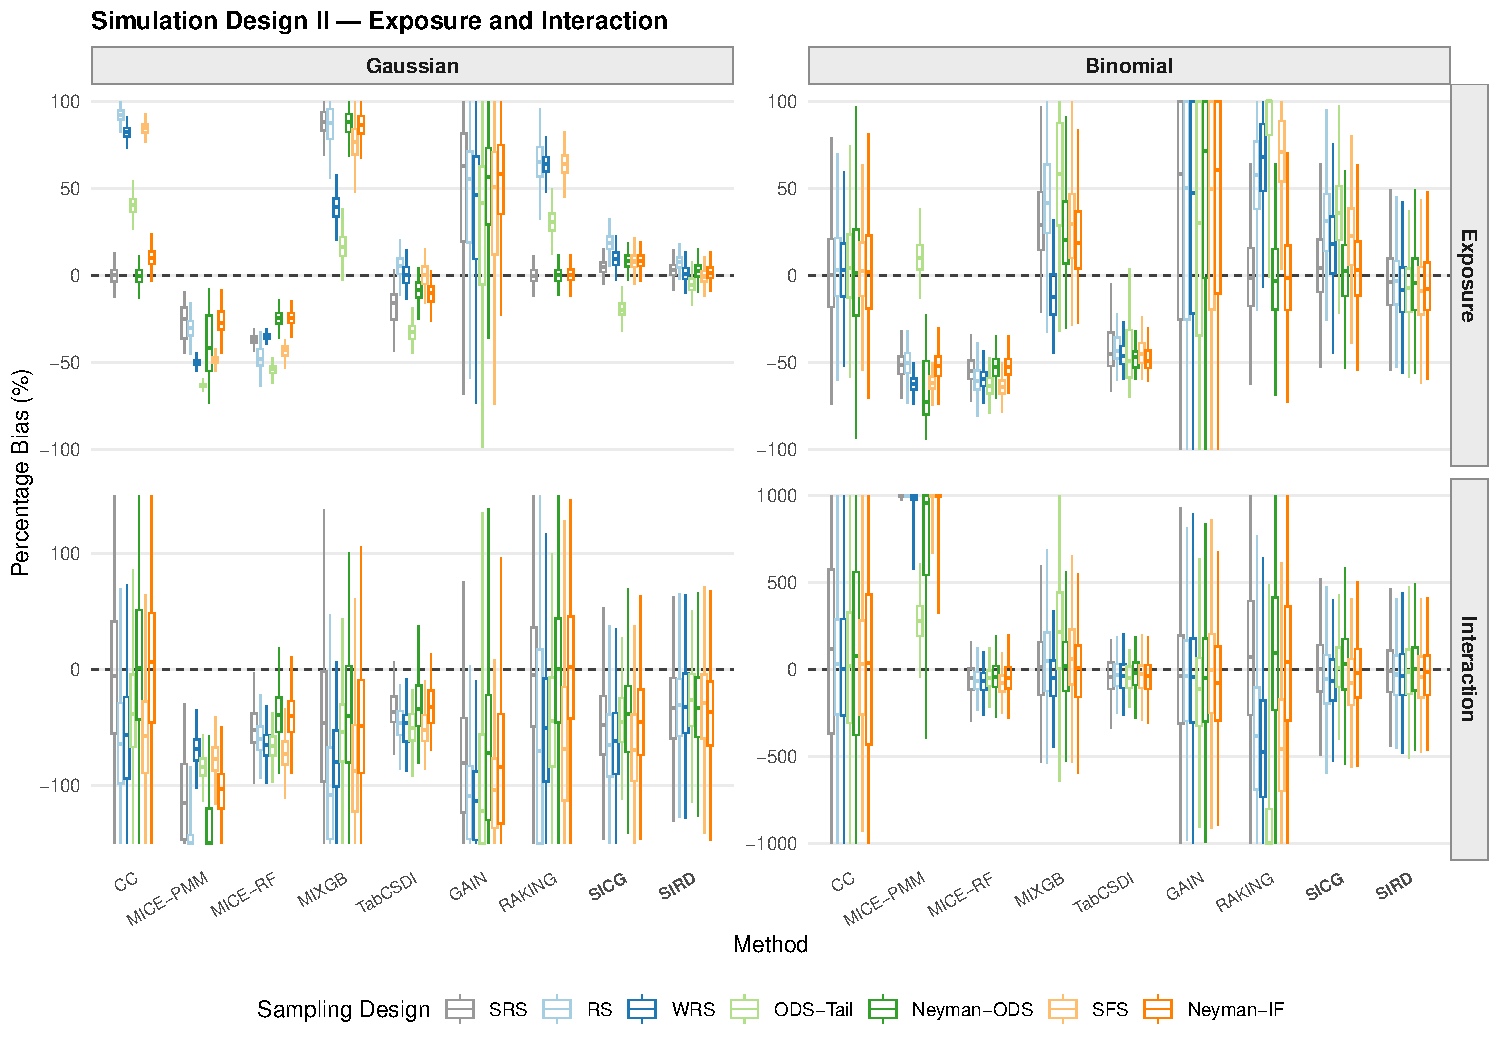
\includegraphics[width=\linewidth,height=0.86\textheight,keepaspectratio]{simI_focal_pctbias.pdf}
\caption{Per-replicate percentage bias of the exposure and the interaction, Simulation Design~II, by imputation method and sampling design (Gaussian and Binomial models). The dashed line marks zero bias; SICG and SIRD are shown in bold.}
\label{fig:appc_simI_focal}
\end{figure}
\end{landscape}
\clearpage

\begin{landscape}
\begin{figure}[p]
\centering
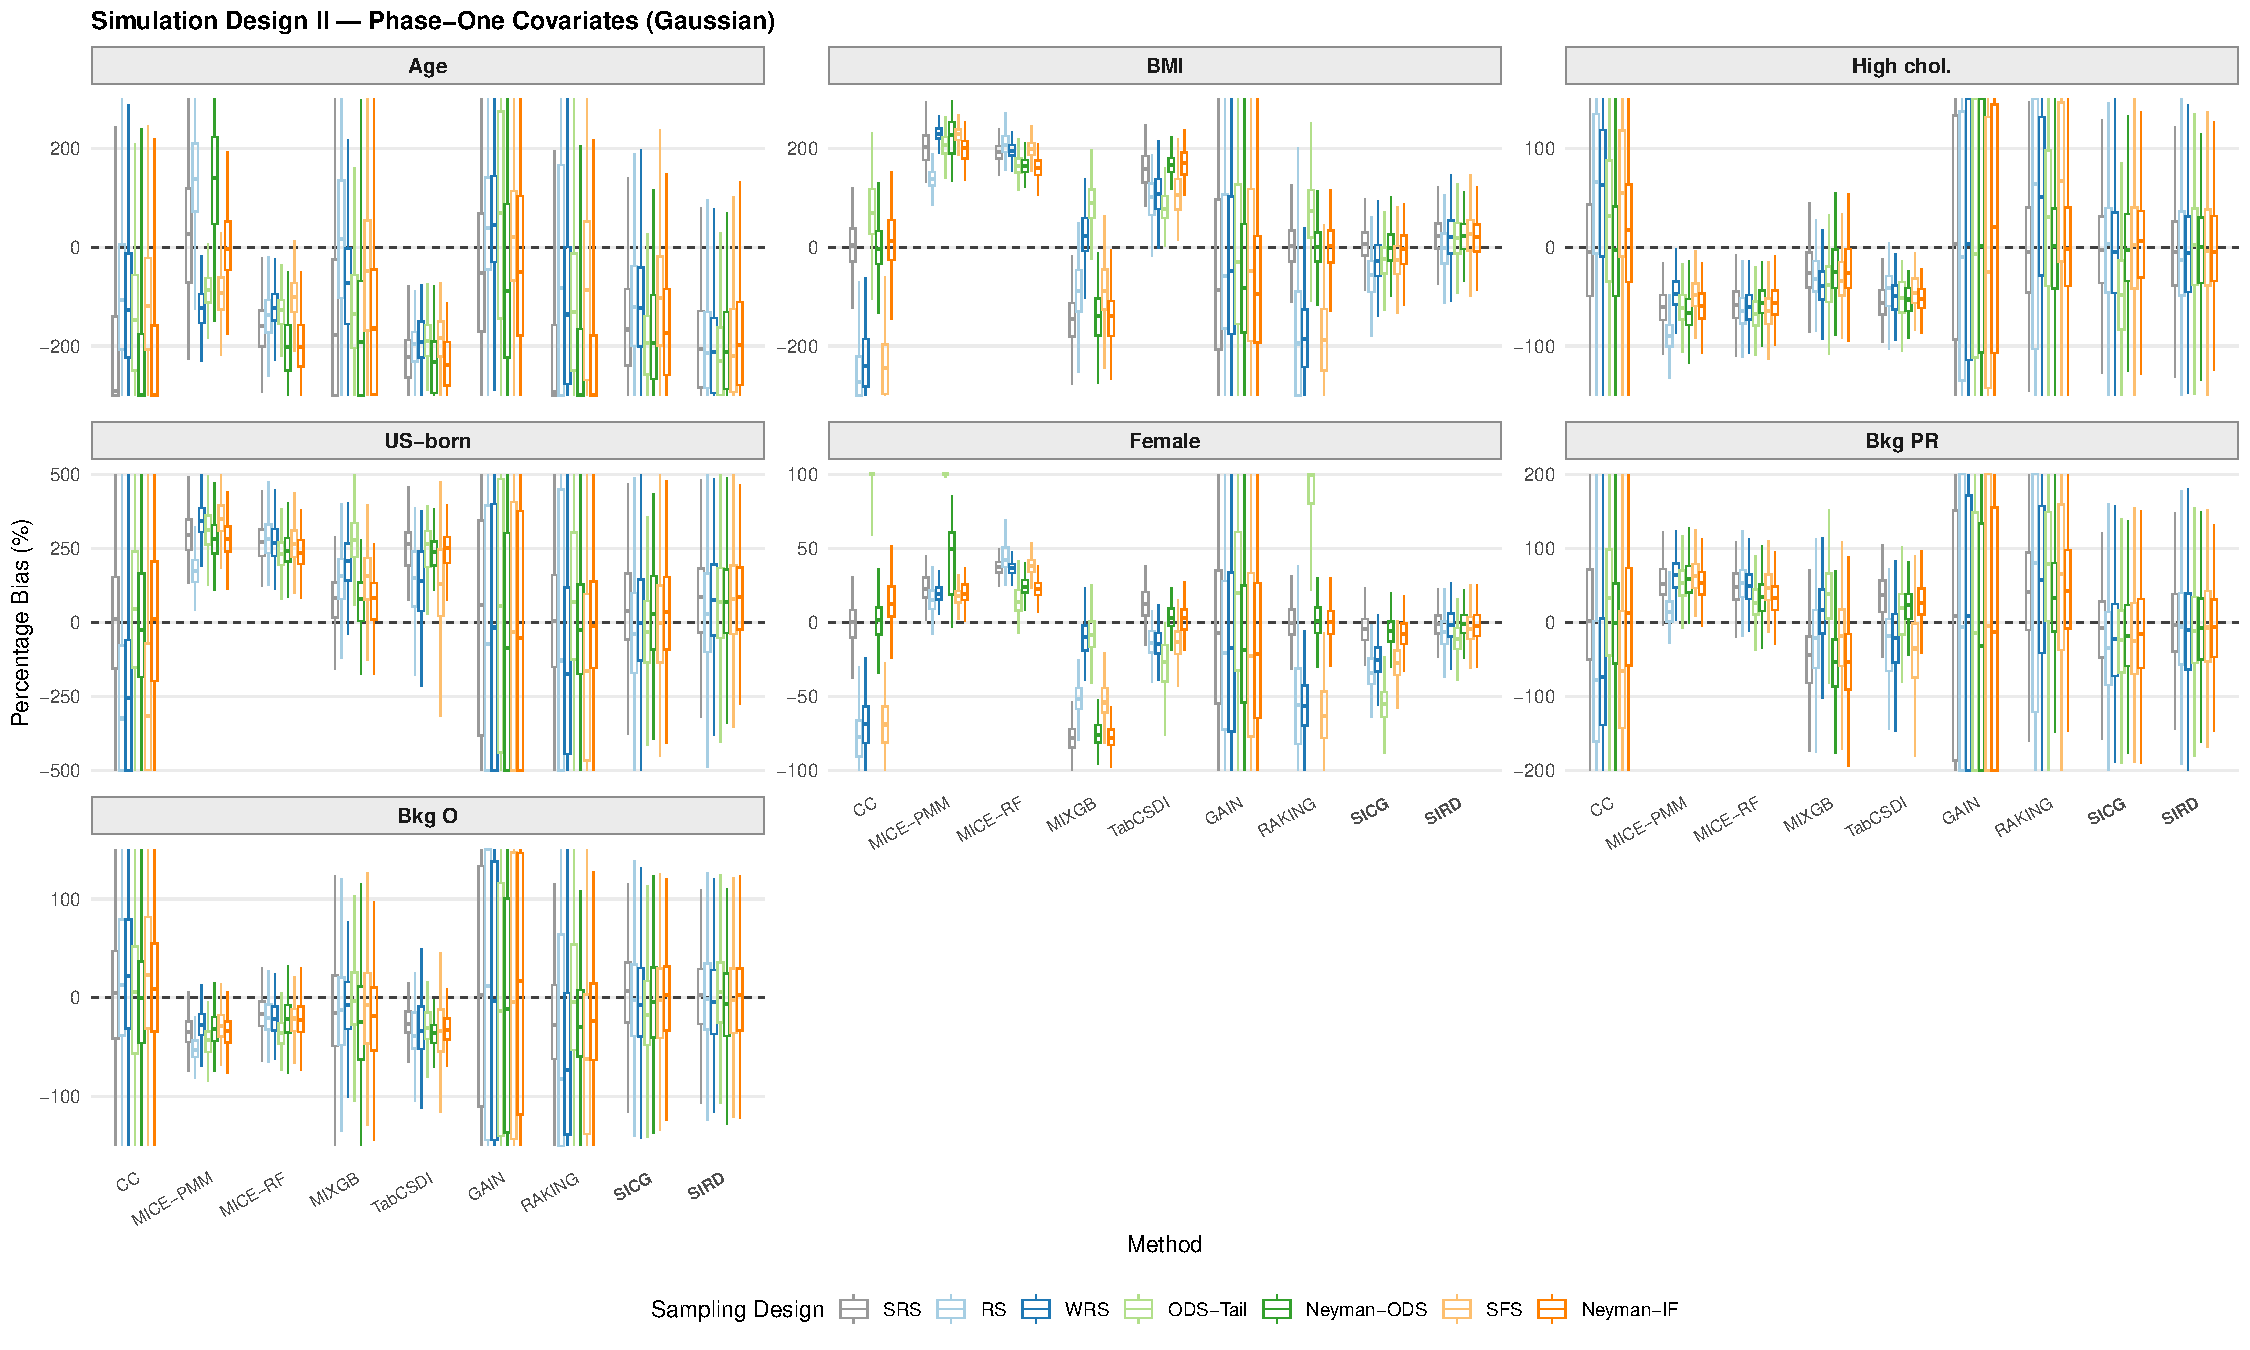
\includegraphics[width=\linewidth,height=0.86\textheight,keepaspectratio]{simI_phase1cov_gaussian_pctbias.pdf}
\caption{Per-replicate percentage bias of the Phase-One (fully observed) covariates, Simulation Design~II, Gaussian model.}
\label{fig:appc_simI_p1_gauss}
\end{figure}
\end{landscape}
\clearpage

\begin{landscape}
\begin{figure}[p]
\centering
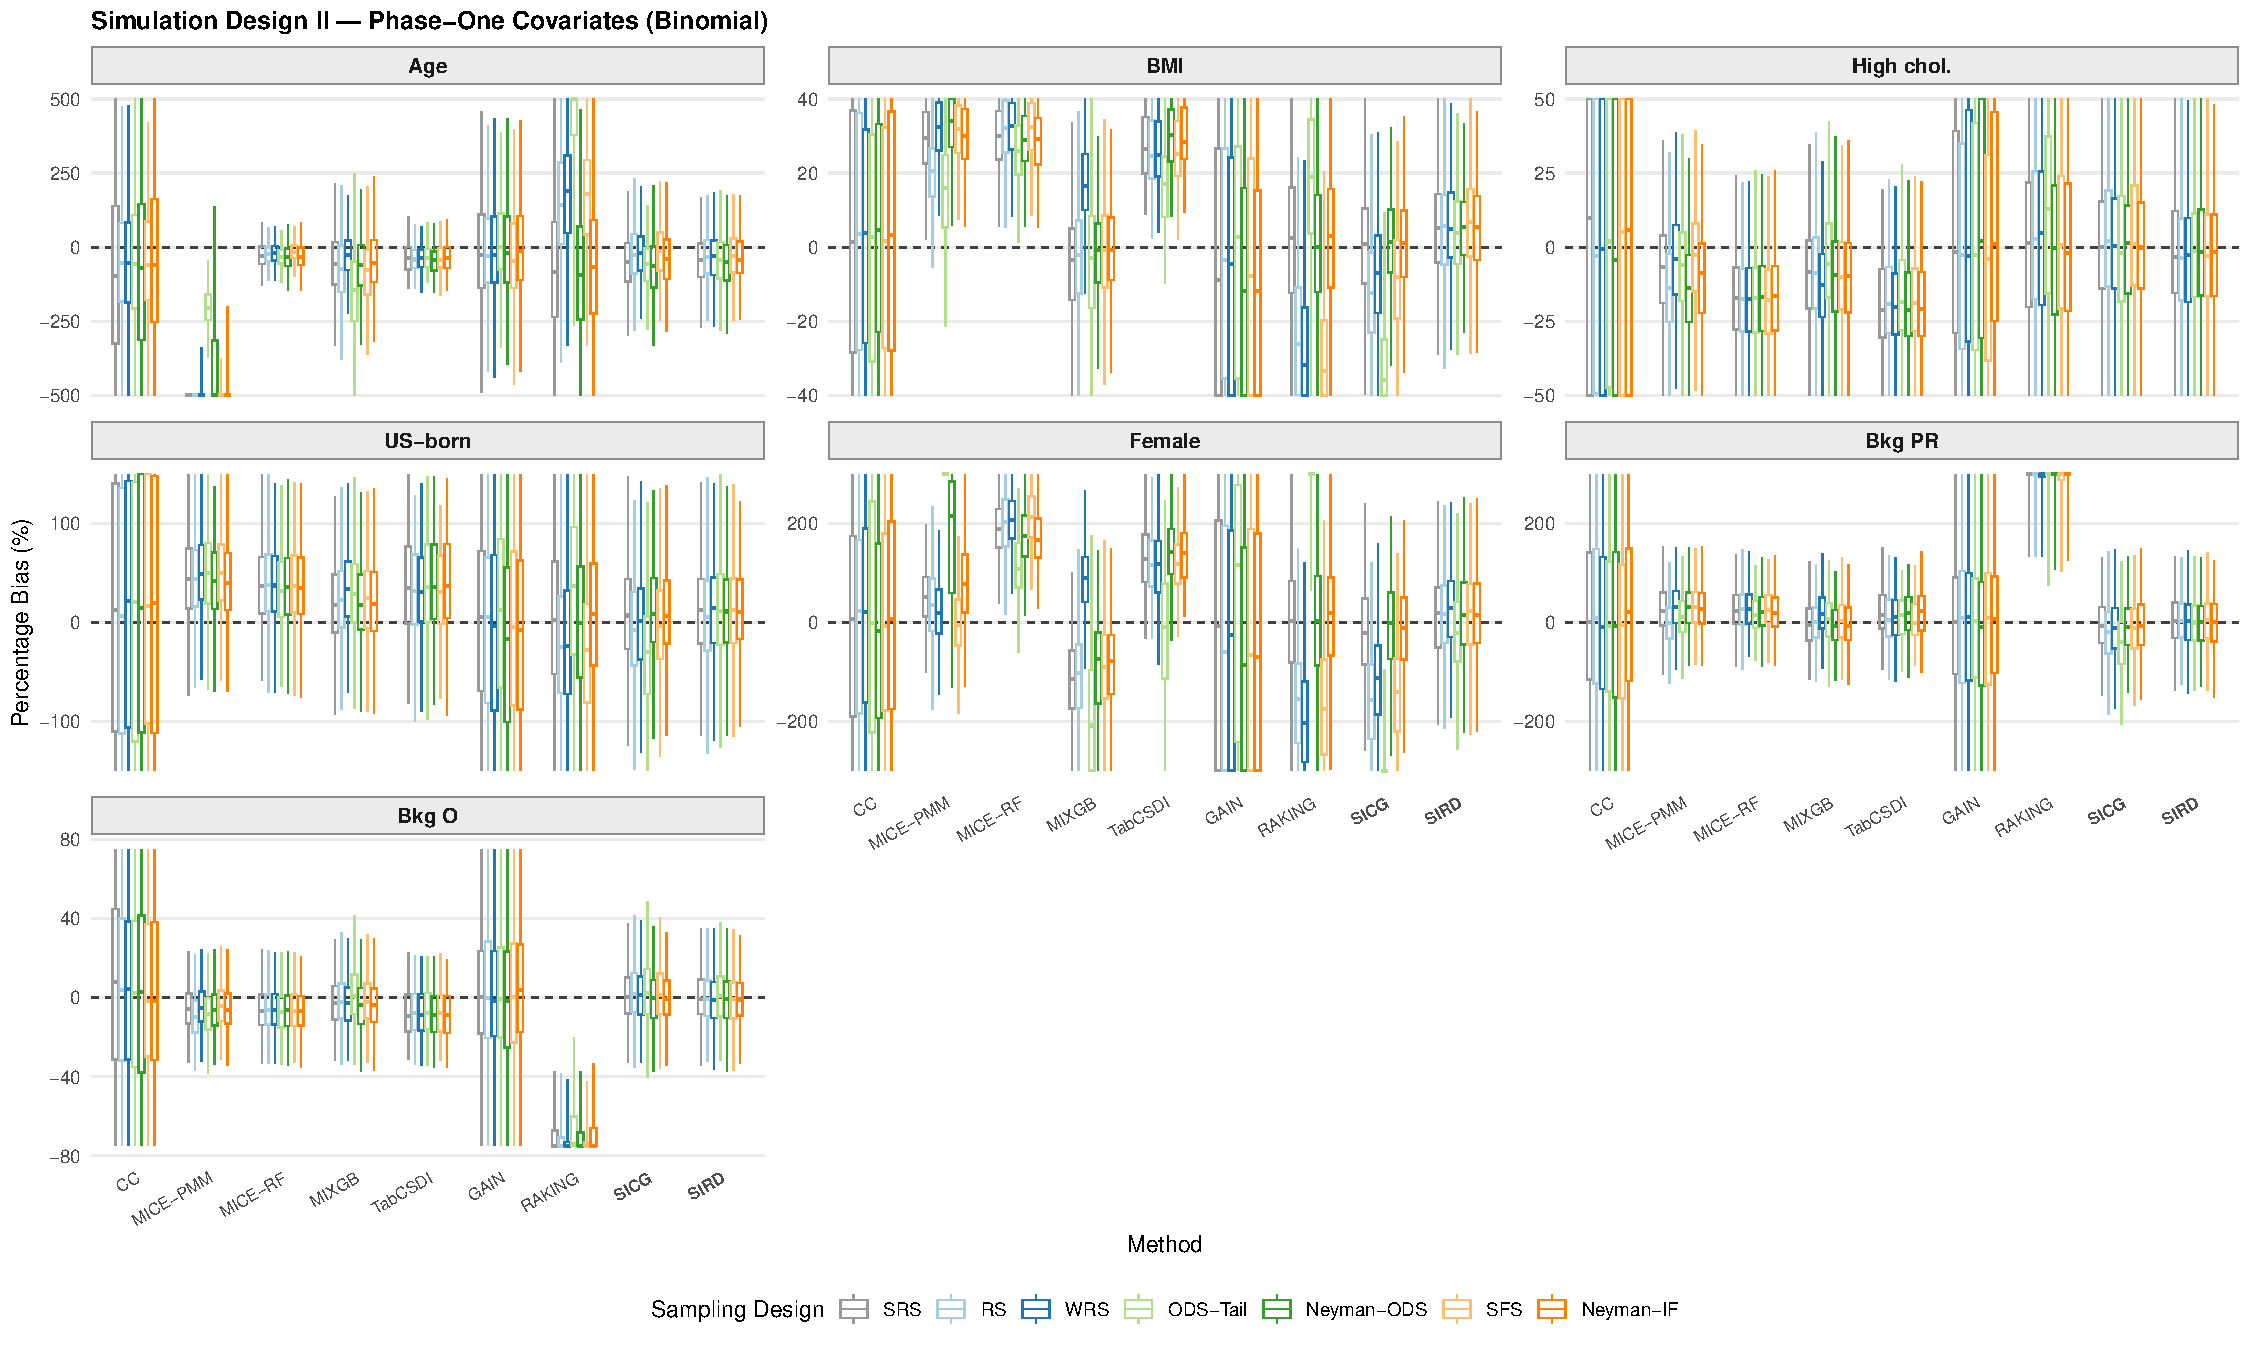
\includegraphics[width=\linewidth,height=0.86\textheight,keepaspectratio]{simI_phase1cov_binomial_pctbias.pdf}
\caption{Per-replicate percentage bias of the Phase-One (fully observed) covariates, Simulation Design~II, Binomial model.}
\label{fig:appc_simI_p1_binom}
\end{figure}
\end{landscape}
\clearpage

\subsection{Imputed exposure distributions}

This companion to Figure~\ref{fig:gain_underdispersion} extends the same single-replicate diagnostic to every imputation method under Simulation Design~II.

\begin{landscape}
\begin{figure}[p]
\centering
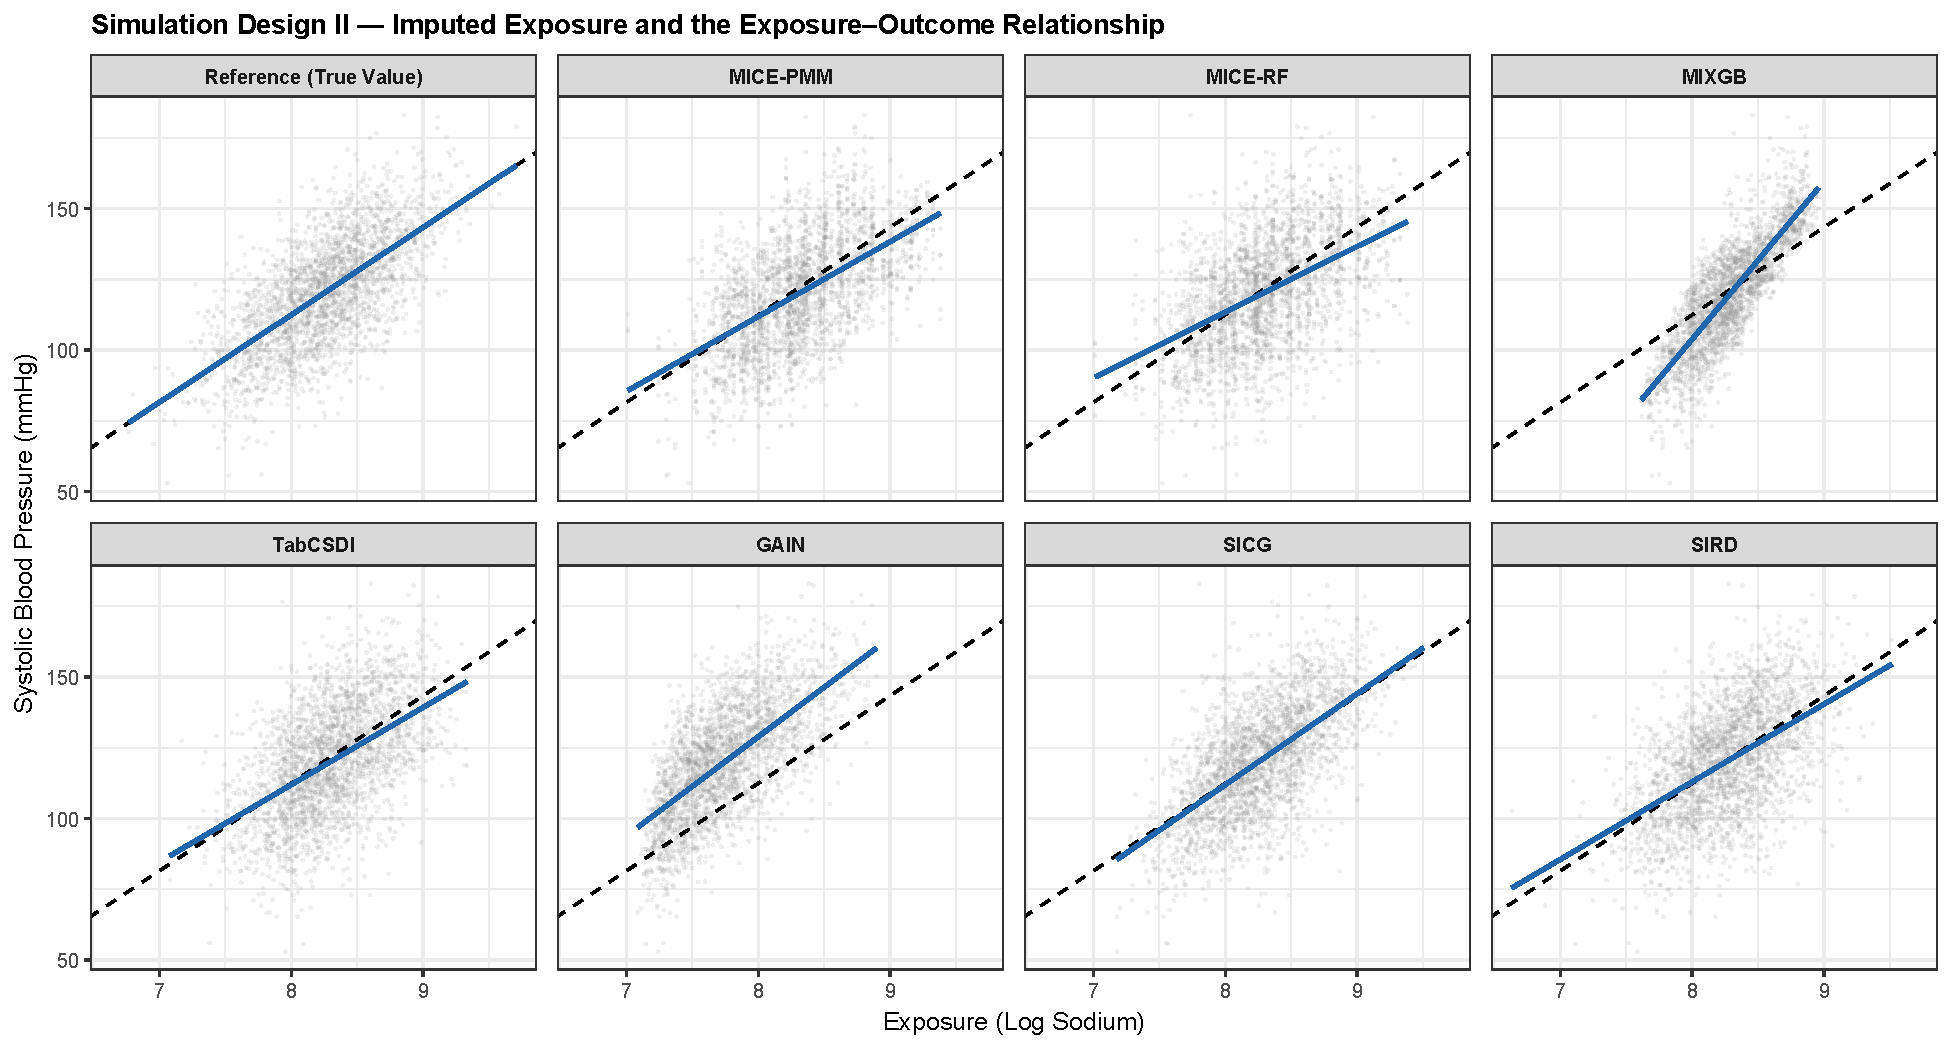
\includegraphics[width=\linewidth,height=0.86\textheight,keepaspectratio]{simII_imputation_dispersion.pdf}
\caption{Imputed exposure and the exposure--outcome relationship under Simulation Design~II, for the first imputation of a single replicate under simple random sampling. Each panel plots the Gaussian outcome against the exposure for the unvalidated units; the reference panel uses the true exposure. The dashed line is the true regression fit, repeated in every panel, and the solid line is the fit within each panel. Where the imputed exposure is concentrated near its conditional mean its spread is compressed and the within-panel line steepens away from the dashed reference, the mechanism described for Figure~\ref{fig:gain_underdispersion}; the distortion is most severe for MIXGB and mildest for SICG and SIRD.}
\label{fig:appc_simI_dispersion}
\end{figure}
\end{landscape}
\clearpage

\FloatBarrier

\clearpage
\section{Simulation Design~III}
\label{app:suppC_simII}

This section collects the full supplementary results for Simulation Design~III, the high-dimensional survival design of Chapter~\ref{chap:SIRD}, targeting a Cox proportional hazards model. Results are reported under the two error mechanisms, \texttt{SampleE} (covariate error) and \texttt{SampleOE} (covariate and outcome error), by coefficient group, separating the imputed Phase-Two covariates from the fully observed Phase-One covariates; the full per-design metric tables appear first, followed by the per-replicate percentage-bias figures.

\subsection{Full per-design metrics}

\begin{landscape}
\definecolor{rankone}{RGB}{33,113,181}\definecolor{ranktwo}{RGB}{107,174,214}\definecolor{rankthree}{RGB}{198,219,239}
\footnotesize\setlength{\tabcolsep}{3.5pt}
\begin{longtable}{llrrrrrrrrrr}
\caption{Full simulation metrics for Simulation Design~III, \texttt{SampleE} (covariate error), over all sampling designs. Metrics, aggregation and shading as in Table~\ref{tab:appc_nutri_Gaussian}.}
\label{tab:appc_surv_SampleE} \\
\toprule
Design & Metric & \multicolumn{1}{c}{CC} & \multicolumn{1}{c}{UNVAL} & \multicolumn{1}{c}{MICE-PMM} & \multicolumn{1}{c}{MICE-RF} & \multicolumn{1}{c}{MIXGB} & \multicolumn{1}{c}{TabCSDI} & \multicolumn{1}{c}{GAIN} & \multicolumn{1}{c}{RAKING} & \multicolumn{1}{c}{\textbf{SICG}} & \multicolumn{1}{c}{\textbf{SIRD}} \\
\midrule
\endfirsthead
\multicolumn{12}{l}{\footnotesize\itshape Table~\ref{tab:appc_surv_SampleE} (continued)} \\
\toprule
Design & Metric & \multicolumn{1}{c}{CC} & \multicolumn{1}{c}{UNVAL} & \multicolumn{1}{c}{MICE-PMM} & \multicolumn{1}{c}{MICE-RF} & \multicolumn{1}{c}{MIXGB} & \multicolumn{1}{c}{TabCSDI} & \multicolumn{1}{c}{GAIN} & \multicolumn{1}{c}{RAKING} & \multicolumn{1}{c}{\textbf{SICG}} & \multicolumn{1}{c}{\textbf{SIRD}} \\
\midrule
\endhead
\midrule \multicolumn{12}{r}{\footnotesize\itshape continued on next page} \\
\endfoot
\bottomrule
\endlastfoot
\multicolumn{12}{l}{\textbf{Continuous Phase-Two Covariates}} \\
\addlinespace[2pt]
\quad \texttt{SRS} & Mean $|$Bias$|$ (\%) & \cellcolor{rankone}0.2 & 6.2 & 1.9 & 4.3 & 2.0 &  & 7.2 & \cellcolor{ranktwo}0.3 & \cellcolor{rankthree}1.4 & \cellcolor{rankthree}1.4 \\
 & Rel.\ RMSE (\%) & 4.5 & 6.5 & 3.2 & 4.4 & \cellcolor{rankthree}3.0 &  & 19.5 & 3.6 & \cellcolor{ranktwo}2.7 & \cellcolor{rankone}2.0 \\
 & Emp.\ SE & 0.051 & 0.013 & 0.033 & 0.008 & 0.017 &  & 0.183 & 0.043 & 0.024 & 0.015 \\
 & Mean SE & 0.051 & 0.011 & 0.027 & 0.016 & 0.014 &  & 0.017 & 0.040 & 0.015 & 0.018 \\
 & SE ratio & \cellcolor{rankone}1.00 & \cellcolor{rankthree}0.85 & 0.82 & 2.00 & 0.82 &  & 0.09 & \cellcolor{ranktwo}0.93 & 0.62 & 1.20 \\
 & Nom.\ Cov. & \cellcolor{rankone}0.95 & 0.15 & 0.70 & 0.11 & 0.46 &  & 0.12 & \cellcolor{ranktwo}0.93 & 0.57 & \cellcolor{rankthree}0.89 \\
 & Orc.\ Cov.\ (Emp) & \cellcolor{rankone}0.95 & 0.17 & 0.75 & 0.04 & 0.54 &  & \cellcolor{ranktwo}0.88 & \cellcolor{rankone}0.95 & 0.71 & \cellcolor{rankthree}0.80 \\
 & Orc.\ Cov.\ (BC) & \cellcolor{rankone}0.95 & 0.91 & \cellcolor{rankthree}0.92 & 0.99 & 0.89 &  & 0.19 & \cellcolor{ranktwo}0.93 & 0.82 & \cellcolor{rankthree}0.98 \\
\addlinespace[2pt]
\quad \texttt{Balanced} & Mean $|$Bias$|$ (\%) & 3.5 & 6.2 & 2.1 & 4.5 & \cellcolor{rankthree}1.7 &  & 2.0 & \cellcolor{rankone}0.2 & \cellcolor{ranktwo}1.2 & \cellcolor{rankthree}1.7 \\
 & Rel.\ RMSE (\%) & 4.5 & 6.5 & 3.2 & 4.6 & \cellcolor{rankthree}2.7 &  & 11.6 & 3.1 & \cellcolor{ranktwo}2.5 & \cellcolor{rankone}2.2 \\
 & Emp.\ SE & 0.028 & 0.013 & 0.032 & 0.008 & 0.016 &  & 0.121 & 0.037 & 0.024 & 0.015 \\
 & Mean SE & 0.028 & 0.011 & 0.023 & 0.015 & 0.013 &  & 0.012 & 0.034 & 0.015 & 0.022 \\
 & SE ratio & \cellcolor{rankone}1.00 & \cellcolor{rankthree}0.85 & 0.72 & 1.88 & 0.81 &  & 0.10 & \cellcolor{ranktwo}0.92 & 0.62 & 1.47 \\
 & Nom.\ Cov. & 0.60 & 0.15 & \cellcolor{rankthree}0.67 & 0.08 & 0.49 &  & 0.16 & \cellcolor{rankone}0.91 & 0.63 & \cellcolor{ranktwo}0.87 \\
 & Orc.\ Cov.\ (Emp) & 0.62 & 0.17 & 0.71 & 0.02 & 0.57 &  & \cellcolor{ranktwo}0.86 & \cellcolor{rankone}0.95 & \cellcolor{rankthree}0.75 & 0.70 \\
 & Orc.\ Cov.\ (BC) & \cellcolor{rankone}0.94 & \cellcolor{ranktwo}0.91 & 0.89 & \cellcolor{rankthree}1.00 & 0.88 &  & 0.17 & \cellcolor{ranktwo}0.91 & 0.83 & \cellcolor{ranktwo}0.99 \\
\addlinespace[2pt]
\quad \texttt{Neyman-IF} & Mean $|$Bias$|$ (\%) & 3.1 & 6.2 & \cellcolor{rankthree}1.6 & 4.2 & 1.8 &  & 3.0 & \cellcolor{rankone}0.1 & \cellcolor{ranktwo}1.0 & 1.7 \\
 & Rel.\ RMSE (\%) & 4.3 & 6.5 & 2.7 & 4.3 & 2.8 &  & 12.6 & \cellcolor{ranktwo}2.5 & \cellcolor{rankone}2.3 & \cellcolor{rankthree}2.6 \\
 & Emp.\ SE & 0.028 & 0.013 & 0.028 & 0.008 & 0.015 &  & 0.120 & 0.030 & 0.022 & 0.015 \\
 & Mean SE & 0.028 & 0.011 & 0.023 & 0.016 & 0.012 &  & 0.012 & 0.028 & 0.016 & 0.024 \\
 & SE ratio & \cellcolor{rankone}1.00 & \cellcolor{rankthree}0.85 & 0.82 & 2.00 & 0.80 &  & 0.10 & \cellcolor{ranktwo}0.93 & 0.73 & 1.60 \\
 & Nom.\ Cov. & 0.61 & 0.15 & 0.73 & 0.16 & 0.44 &  & 0.15 & \cellcolor{rankone}0.92 & \cellcolor{rankthree}0.75 & \cellcolor{ranktwo}0.83 \\
 & Orc.\ Cov.\ (Emp) & 0.59 & 0.17 & 0.77 & 0.04 & 0.51 &  & \cellcolor{ranktwo}0.79 & \cellcolor{rankone}0.94 & \cellcolor{rankthree}0.78 & 0.57 \\
 & Orc.\ Cov.\ (BC) & \cellcolor{rankone}0.95 & \cellcolor{rankthree}0.91 & \cellcolor{rankthree}0.91 & 1.00 & 0.89 &  & 0.17 & \cellcolor{ranktwo}0.93 & 0.88 & \cellcolor{rankthree}0.99 \\
\addlinespace[2pt]
\multicolumn{12}{l}{\textbf{Binary \& Categorical Phase-Two Covariates}} \\
\addlinespace[2pt]
\quad \texttt{SRS} & Mean $|$Bias$|$ (\%) & 4.3 & 6.5 & 8.8 & \cellcolor{rankone}2.6 & \cellcolor{rankthree}3.4 &  & 12.9 & \cellcolor{ranktwo}3.3 & 4.5 & 3.7 \\
 & Rel.\ RMSE (\%) & 31.3 & 9.7 & 17.4 & \cellcolor{rankone}7.9 & \cellcolor{ranktwo}8.9 &  & 59.3 & 27.9 & 11.5 & \cellcolor{rankthree}9.0 \\
 & Emp.\ SE & 0.299 & 0.055 & 0.121 & 0.051 & 0.083 &  & 0.423 & 0.266 & 0.106 & 0.060 \\
 & Mean SE & 0.314 & 0.054 & 0.113 & 0.097 & 0.080 &  & 0.079 & 0.260 & 0.092 & 0.120 \\
 & SE ratio & \cellcolor{rankthree}1.05 & \cellcolor{rankone}0.98 & 0.93 & 1.90 & \cellcolor{ranktwo}0.96 &  & 0.19 & \cellcolor{rankone}0.98 & 0.87 & 2.00 \\
 & Nom.\ Cov. & \cellcolor{ranktwo}0.97 & 0.61 & 0.80 & \cellcolor{rankthree}0.99 & \cellcolor{rankthree}0.91 &  & 0.30 & \cellcolor{rankone}0.94 & 0.88 & \cellcolor{rankthree}0.99 \\
 & Orc.\ Cov.\ (Emp) & \cellcolor{rankone}0.95 & 0.65 & \cellcolor{rankthree}0.86 & 0.72 & \cellcolor{ranktwo}0.92 &  & \cellcolor{rankone}0.95 & \cellcolor{rankone}0.95 & \cellcolor{ranktwo}0.92 & 0.78 \\
 & Orc.\ Cov.\ (BC) & \cellcolor{rankthree}0.97 & \cellcolor{rankone}0.95 & \cellcolor{rankthree}0.93 & 0.99 & \cellcolor{rankthree}0.93 &  & 0.31 & \cellcolor{ranktwo}0.94 & 0.91 & 0.99 \\
\addlinespace[2pt]
\quad \texttt{Balanced} & Mean $|$Bias$|$ (\%) & 2.7 & 6.5 & 34.9 & \cellcolor{rankone}0.9 & \cellcolor{rankthree}1.3 &  & 5.0 & \cellcolor{ranktwo}1.1 & 2.5 & 1.6 \\
 & Rel.\ RMSE (\%) & 15.3 & 9.7 & 40.7 & \cellcolor{rankone}5.8 & \cellcolor{rankthree}7.4 &  & 28.1 & 19.4 & 10.0 & \cellcolor{ranktwo}6.4 \\
 & Emp.\ SE & 0.142 & 0.055 & 0.142 & 0.054 & 0.076 &  & 0.258 & 0.191 & 0.097 & 0.058 \\
 & Mean SE & 0.143 & 0.054 & 0.094 & 0.089 & 0.072 &  & 0.064 & 0.177 & 0.088 & 0.100 \\
 & SE ratio & \cellcolor{rankone}1.01 & \cellcolor{ranktwo}0.98 & 0.66 & 1.65 & \cellcolor{rankthree}0.95 &  & 0.25 & 0.93 & 0.91 & 1.72 \\
 & Nom.\ Cov. & \cellcolor{rankone}0.94 & 0.61 & 0.26 & \cellcolor{rankthree}0.99 & \cellcolor{ranktwo}0.93 &  & 0.37 & \cellcolor{ranktwo}0.93 & \cellcolor{rankthree}0.91 & \cellcolor{rankthree}0.99 \\
 & Orc.\ Cov.\ (Emp) & \cellcolor{ranktwo}0.94 & 0.65 & 0.40 & \cellcolor{rankthree}0.93 & \cellcolor{rankone}0.95 &  & \cellcolor{rankone}0.95 & \cellcolor{rankone}0.95 & \cellcolor{rankthree}0.93 & 0.90 \\
 & Orc.\ Cov.\ (BC) & \cellcolor{ranktwo}0.96 & \cellcolor{rankone}0.95 & 0.82 & 0.99 & \cellcolor{rankthree}0.93 &  & 0.39 & \cellcolor{rankthree}0.93 & 0.91 & 0.99 \\
\addlinespace[2pt]
\quad \texttt{Neyman-IF} & Mean $|$Bias$|$ (\%) & 2.5 & 6.5 & 30.8 & \cellcolor{ranktwo}1.3 & 1.9 &  & 6.7 & \cellcolor{rankthree}1.6 & 3.6 & \cellcolor{rankone}1.0 \\
 & Rel.\ RMSE (\%) & 18.8 & 9.7 & 36.7 & \cellcolor{ranktwo}7.1 & \cellcolor{rankthree}8.7 &  & 34.7 & 18.0 & 11.3 & \cellcolor{rankone}6.8 \\
 & Emp.\ SE & 0.169 & 0.055 & 0.142 & 0.067 & 0.090 &  & 0.287 & 0.180 & 0.105 & 0.066 \\
 & Mean SE & 0.169 & 0.054 & 0.095 & 0.110 & 0.079 &  & 0.077 & 0.170 & 0.094 & 0.116 \\
 & SE ratio & \cellcolor{rankone}1.00 & \cellcolor{ranktwo}0.98 & 0.67 & 1.64 & 0.88 &  & 0.27 & \cellcolor{rankthree}0.94 & 0.90 & 1.76 \\
 & Nom.\ Cov. & \cellcolor{rankone}0.93 & 0.61 & 0.28 & \cellcolor{ranktwo}0.99 & \cellcolor{ranktwo}0.91 &  & 0.39 & \cellcolor{rankone}0.93 & \cellcolor{rankthree}0.90 & \cellcolor{ranktwo}0.99 \\
 & Orc.\ Cov.\ (Emp) & \cellcolor{rankthree}0.93 & 0.65 & 0.46 & \cellcolor{rankthree}0.93 & \cellcolor{ranktwo}0.94 &  & \cellcolor{ranktwo}0.94 & \cellcolor{rankone}0.95 & \cellcolor{rankthree}0.93 & \cellcolor{rankthree}0.93 \\
 & Orc.\ Cov.\ (BC) & \cellcolor{rankone}0.95 & \cellcolor{rankone}0.95 & 0.84 & 1.00 & \cellcolor{rankthree}0.92 &  & 0.43 & \cellcolor{ranktwo}0.93 & \cellcolor{rankthree}0.92 & 0.99 \\
\addlinespace[2pt]
\multicolumn{12}{l}{\textbf{Continuous Phase-One Covariates}} \\
\addlinespace[2pt]
\quad \texttt{SRS} & Mean $|$Bias$|$ (\%) & \cellcolor{ranktwo}0.5 & 31.6 & 4.3 & \cellcolor{rankone}0.1 & 0.8 &  & 7.4 & \cellcolor{rankthree}0.7 & \cellcolor{rankone}0.1 & 3.2 \\
 & Rel.\ RMSE (\%) & 5.3 & 31.7 & 4.9 & \cellcolor{rankone}1.1 & \cellcolor{rankthree}1.8 &  & 11.2 & 3.5 & \cellcolor{ranktwo}1.4 & 3.5 \\
 & Emp.\ SE & 0.052 & 0.023 & 0.024 & 0.011 & 0.016 &  & 0.079 & 0.035 & 0.014 & 0.015 \\
 & Mean SE & 0.051 & 0.020 & 0.020 & 0.012 & 0.014 &  & 0.021 & 0.030 & 0.012 & 0.017 \\
 & SE ratio & \cellcolor{rankone}0.98 & 0.87 & 0.83 & \cellcolor{ranktwo}1.09 & \cellcolor{rankthree}0.88 &  & 0.27 & 0.86 & 0.86 & 1.13 \\
 & Nom.\ Cov. & \cellcolor{rankone}0.95 & 0.00 & 0.43 & \cellcolor{ranktwo}0.98 & 0.89 &  & 0.26 & \cellcolor{ranktwo}0.92 & \cellcolor{rankthree}0.90 & 0.61 \\
 & Orc.\ Cov.\ (Emp) & \cellcolor{ranktwo}0.96 & 0.00 & 0.53 & \cellcolor{ranktwo}0.96 & \cellcolor{rankthree}0.93 &  & 0.87 & \cellcolor{rankone}0.95 & \cellcolor{ranktwo}0.96 & 0.48 \\
 & Orc.\ Cov.\ (BC) & \cellcolor{rankone}0.95 & 0.91 & 0.88 & \cellcolor{rankthree}0.98 & 0.90 &  & 0.41 & \cellcolor{rankthree}0.92 & 0.91 & \cellcolor{ranktwo}0.97 \\
\addlinespace[2pt]
\quad \texttt{Balanced} & Mean $|$Bias$|$ (\%) & 11.3 & 31.6 & 2.8 & \cellcolor{rankone}0.2 & 0.9 &  & \cellcolor{rankthree}0.8 & \cellcolor{rankone}0.2 & \cellcolor{ranktwo}0.3 & 1.8 \\
 & Rel.\ RMSE (\%) & 11.5 & 31.7 & 3.3 & \cellcolor{rankone}1.1 & \cellcolor{rankthree}1.7 &  & 6.4 & 2.8 & \cellcolor{ranktwo}1.4 & 2.3 \\
 & Emp.\ SE & 0.024 & 0.023 & 0.019 & 0.011 & 0.015 &  & 0.064 & 0.028 & 0.014 & 0.015 \\
 & Mean SE & 0.027 & 0.020 & 0.016 & 0.012 & 0.013 &  & 0.012 & 0.025 & 0.011 & 0.019 \\
 & SE ratio & \cellcolor{rankthree}1.12 & 0.87 & 0.84 & \cellcolor{rankone}1.09 & 0.87 &  & 0.19 & \cellcolor{ranktwo}0.89 & 0.79 & 1.27 \\
 & Nom.\ Cov. & 0.00 & 0.00 & 0.58 & \cellcolor{rankone}0.96 & 0.87 &  & 0.28 & \cellcolor{ranktwo}0.91 & 0.88 & \cellcolor{rankthree}0.90 \\
 & Orc.\ Cov.\ (Emp) & 0.00 & 0.00 & 0.69 & \cellcolor{rankone}0.95 & \cellcolor{rankthree}0.91 &  & \cellcolor{rankone}0.95 & \cellcolor{ranktwo}0.94 & \cellcolor{rankone}0.95 & 0.77 \\
 & Orc.\ Cov.\ (BC) & \cellcolor{rankone}0.97 & \cellcolor{rankthree}0.91 & 0.90 & \cellcolor{rankone}0.97 & \cellcolor{ranktwo}0.92 &  & 0.30 & \cellcolor{ranktwo}0.92 & 0.89 & \cellcolor{rankthree}0.99 \\
\addlinespace[2pt]
\quad \texttt{Neyman-IF} & Mean $|$Bias$|$ (\%) & 11.4 & 31.6 & 3.4 & \cellcolor{rankthree}0.8 & 1.0 &  & 1.4 & \cellcolor{rankone}0.4 & \cellcolor{ranktwo}0.6 & 1.6 \\
 & Rel.\ RMSE (\%) & 11.7 & 31.7 & 3.8 & \cellcolor{rankone}1.3 & \cellcolor{rankthree}1.8 &  & 6.1 & 2.5 & \cellcolor{ranktwo}1.5 & 2.3 \\
 & Emp.\ SE & 0.031 & 0.023 & 0.019 & 0.011 & 0.015 &  & 0.060 & 0.025 & 0.014 & 0.015 \\
 & Mean SE & 0.028 & 0.020 & 0.016 & 0.012 & 0.012 &  & 0.012 & 0.022 & 0.012 & 0.019 \\
 & SE ratio & \cellcolor{ranktwo}0.90 & 0.87 & 0.84 & \cellcolor{rankone}1.09 & 0.80 &  & 0.20 & \cellcolor{rankthree}0.88 & 0.86 & 1.27 \\
 & Nom.\ Cov. & 0.01 & 0.00 & 0.44 & \cellcolor{ranktwo}0.91 & 0.81 &  & 0.30 & \cellcolor{ranktwo}0.91 & \cellcolor{rankthree}0.86 & \cellcolor{rankone}0.92 \\
 & Orc.\ Cov.\ (Emp) & 0.01 & 0.00 & 0.55 & 0.89 & \cellcolor{rankthree}0.90 &  & \cellcolor{rankone}0.95 & \cellcolor{rankone}0.95 & \cellcolor{ranktwo}0.93 & 0.81 \\
 & Orc.\ Cov.\ (BC) & \cellcolor{rankone}0.93 & \cellcolor{ranktwo}0.91 & \cellcolor{ranktwo}0.91 & \cellcolor{rankone}0.97 & \cellcolor{rankthree}0.90 &  & 0.34 & \cellcolor{ranktwo}0.91 & \cellcolor{rankthree}0.90 & \cellcolor{ranktwo}0.99 \\
\addlinespace[2pt]
\multicolumn{12}{l}{\textbf{Binary \& Categorical Phase-One Covariates}} \\
\addlinespace[2pt]
\quad \texttt{SRS} & Mean $|$Bias$|$ (\%) & 3.2 & 2.7 & 4.5 & 6.8 & 3.7 &  & 7.3 & \cellcolor{rankthree}2.3 & \cellcolor{ranktwo}1.6 & \cellcolor{rankone}1.5 \\
 & Rel.\ RMSE (\%) & 31.2 & \cellcolor{ranktwo}7.4 & 12.7 & 9.8 & \cellcolor{rankthree}7.8 &  & 36.3 & 20.1 & 8.7 & \cellcolor{rankone}6.9 \\
 & Emp.\ SE & 0.311 & 0.061 & 0.141 & 0.056 & 0.066 &  & 0.410 & 0.214 & 0.098 & 0.066 \\
 & Mean SE & 0.304 & 0.059 & 0.127 & 0.079 & 0.061 &  & 0.064 & 0.192 & 0.078 & 0.074 \\
 & SE ratio & \cellcolor{rankone}0.98 & \cellcolor{ranktwo}0.97 & 0.90 & 1.41 & \cellcolor{rankthree}0.92 &  & 0.16 & 0.90 & 0.80 & 1.12 \\
 & Nom.\ Cov. & \cellcolor{rankone}0.95 & 0.85 & \cellcolor{rankthree}0.92 & 0.81 & 0.86 &  & 0.30 & \cellcolor{rankthree}0.92 & 0.89 & \cellcolor{ranktwo}0.96 \\
 & Orc.\ Cov.\ (Emp) & \cellcolor{rankone}0.95 & 0.87 & 0.92 & 0.65 & 0.90 &  & \cellcolor{ranktwo}0.94 & \cellcolor{rankone}0.95 & \cellcolor{ranktwo}0.94 & \cellcolor{rankthree}0.93 \\
 & Orc.\ Cov.\ (BC) & \cellcolor{rankone}0.95 & \cellcolor{rankone}0.95 & \cellcolor{ranktwo}0.94 & 0.99 & \cellcolor{rankthree}0.93 &  & 0.32 & 0.92 & 0.90 & \cellcolor{rankthree}0.97 \\
\addlinespace[2pt]
\quad \texttt{Balanced} & Mean $|$Bias$|$ (\%) & 3.5 & 2.7 & 4.3 & 7.1 & 4.3 &  & 5.0 & \cellcolor{rankone}0.7 & \cellcolor{rankthree}1.2 & \cellcolor{ranktwo}1.0 \\
 & Rel.\ RMSE (\%) & 16.6 & \cellcolor{ranktwo}7.4 & 12.4 & 10.1 & 8.4 &  & 36.4 & 16.5 & \cellcolor{rankthree}8.1 & \cellcolor{rankone}6.7 \\
 & Emp.\ SE & 0.163 & 0.061 & 0.123 & 0.056 & 0.066 &  & 0.370 & 0.178 & 0.093 & 0.064 \\
 & Mean SE & 0.163 & 0.059 & 0.101 & 0.078 & 0.060 &  & 0.064 & 0.164 & 0.080 & 0.081 \\
 & SE ratio & \cellcolor{rankone}1.00 & \cellcolor{ranktwo}0.97 & 0.82 & 1.39 & 0.91 &  & 0.17 & \cellcolor{rankthree}0.92 & 0.86 & 1.27 \\
 & Nom.\ Cov. & \cellcolor{rankone}0.94 & 0.85 & 0.86 & 0.77 & 0.81 &  & 0.36 & \cellcolor{rankthree}0.92 & \cellcolor{rankthree}0.92 & \cellcolor{ranktwo}0.97 \\
 & Orc.\ Cov.\ (Emp) & \cellcolor{ranktwo}0.94 & 0.87 & 0.90 & 0.64 & 0.85 &  & \cellcolor{rankone}0.95 & \cellcolor{rankone}0.95 & \cellcolor{rankone}0.95 & \cellcolor{rankthree}0.93 \\
 & Orc.\ Cov.\ (BC) & \cellcolor{rankone}0.95 & \cellcolor{rankone}0.95 & 0.91 & 0.99 & \cellcolor{rankthree}0.92 &  & 0.36 & \cellcolor{ranktwo}0.93 & \cellcolor{rankthree}0.92 & \cellcolor{rankthree}0.98 \\
\addlinespace[2pt]
\quad \texttt{Neyman-IF} & Mean $|$Bias$|$ (\%) & 1.7 & 2.7 & 4.9 & 7.1 & 4.4 &  & 3.8 & \cellcolor{rankone}0.6 & \cellcolor{rankthree}1.0 & \cellcolor{ranktwo}0.9 \\
 & Rel.\ RMSE (\%) & 17.0 & \cellcolor{ranktwo}7.4 & 11.9 & 10.1 & 8.5 &  & 37.5 & 14.3 & \cellcolor{rankthree}7.9 & \cellcolor{rankone}7.2 \\
 & Emp.\ SE & 0.170 & 0.061 & 0.118 & 0.056 & 0.065 &  & 0.380 & 0.155 & 0.088 & 0.068 \\
 & Mean SE & 0.169 & 0.059 & 0.104 & 0.083 & 0.060 &  & 0.065 & 0.141 & 0.084 & 0.085 \\
 & SE ratio & \cellcolor{rankone}0.99 & \cellcolor{ranktwo}0.97 & 0.88 & 1.48 & 0.92 &  & 0.17 & 0.91 & \cellcolor{rankthree}0.95 & 1.25 \\
 & Nom.\ Cov. & \cellcolor{ranktwo}0.94 & 0.85 & 0.87 & 0.80 & 0.80 &  & 0.32 & \cellcolor{rankthree}0.93 & \cellcolor{ranktwo}0.94 & \cellcolor{rankone}0.95 \\
 & Orc.\ Cov.\ (Emp) & \cellcolor{ranktwo}0.94 & 0.87 & 0.90 & 0.63 & 0.84 &  & \cellcolor{ranktwo}0.96 & \cellcolor{rankone}0.95 & \cellcolor{rankone}0.95 & \cellcolor{rankthree}0.92 \\
 & Orc.\ Cov.\ (BC) & \cellcolor{rankone}0.95 & \cellcolor{rankone}0.95 & \cellcolor{rankthree}0.93 & 0.99 & \cellcolor{rankthree}0.93 &  & 0.32 & \cellcolor{rankthree}0.93 & \cellcolor{ranktwo}0.94 & 0.98 \\
\addlinespace[2pt]
\multicolumn{12}{l}{\textbf{Interaction}} \\
\addlinespace[2pt]
\quad \texttt{SRS} & Mean $|$Bias$|$ (\%) & \cellcolor{ranktwo}0.4 & 5.2 & 5.0 & 6.8 & 2.3 &  & 3.7 & \cellcolor{rankone}0.2 & 5.7 & \cellcolor{rankthree}2.2 \\
 & Rel.\ RMSE (\%) & \cellcolor{ranktwo}1.3 & 5.2 & 5.0 & 6.8 & 2.4 &  & 4.1 & \cellcolor{rankone}1.1 & 5.7 & \cellcolor{rankthree}2.2 \\
 & Emp.\ SE & 0.012 & 0.007 & 0.006 & 0.003 & 0.006 &  & 0.019 & 0.011 & 0.003 & 0.006 \\
 & Mean SE & 0.012 & 0.005 & 0.006 & 0.007 & 0.005 &  & 0.007 & 0.009 & 0.005 & 0.007 \\
 & SE ratio & \cellcolor{rankone}1.00 & 0.71 & \cellcolor{rankone}1.00 & 2.33 & \cellcolor{ranktwo}0.83 &  & 0.37 & \cellcolor{rankthree}0.82 & 1.67 & \cellcolor{ranktwo}1.17 \\
 & Nom.\ Cov. & \cellcolor{rankone}0.94 & 0.00 & 0.00 & 0.00 & 0.01 &  & \cellcolor{rankthree}0.09 & \cellcolor{ranktwo}0.87 & 0.00 & \cellcolor{rankthree}0.09 \\
 & Orc.\ Cov.\ (Emp) & \cellcolor{rankone}0.95 & 0.00 & 0.00 & 0.00 & 0.02 &  & \cellcolor{rankthree}0.49 & \cellcolor{ranktwo}0.94 & 0.00 & 0.02 \\
 & Orc.\ Cov.\ (BC) & \cellcolor{rankone}0.94 & 0.82 & \cellcolor{ranktwo}0.92 & 1.00 & 0.88 &  & 0.71 & 0.88 & \cellcolor{rankthree}0.99 & \cellcolor{rankone}0.96 \\
\addlinespace[2pt]
\quad \texttt{Balanced} & Mean $|$Bias$|$ (\%) & \cellcolor{ranktwo}0.8 & 5.2 & 3.9 & 6.6 & \cellcolor{rankthree}2.0 &  & 7.5 & \cellcolor{rankone}0.2 & 6.0 & 2.8 \\
 & Rel.\ RMSE (\%) & \cellcolor{ranktwo}1.1 & 5.2 & 3.9 & 6.6 & \cellcolor{rankthree}2.1 &  & 7.6 & \cellcolor{rankone}0.9 & 6.0 & 2.9 \\
 & Emp.\ SE & 0.007 & 0.007 & 0.005 & 0.002 & 0.005 &  & 0.014 & 0.009 & 0.003 & 0.006 \\
 & Mean SE & 0.007 & 0.005 & 0.005 & 0.006 & 0.004 &  & 0.002 & 0.007 & 0.005 & 0.009 \\
 & SE ratio & \cellcolor{rankone}1.00 & 0.71 & \cellcolor{rankone}1.00 & 3.00 & \cellcolor{ranktwo}0.80 &  & 0.14 & \cellcolor{rankthree}0.78 & 1.67 & 1.50 \\
 & Nom.\ Cov. & \cellcolor{ranktwo}0.76 & 0.00 & 0.00 & 0.00 & 0.01 &  & 0.00 & \cellcolor{rankone}0.89 & 0.00 & \cellcolor{rankthree}0.09 \\
 & Orc.\ Cov.\ (Emp) & \cellcolor{ranktwo}0.79 & 0.00 & 0.00 & 0.00 & \cellcolor{rankthree}0.01 &  & 0.00 & \cellcolor{rankone}0.94 & 0.00 & 0.00 \\
 & Orc.\ Cov.\ (BC) & \cellcolor{rankone}0.94 & 0.82 & \cellcolor{rankone}0.94 & \cellcolor{rankthree}1.00 & 0.85 &  & 0.12 & 0.89 & \cellcolor{ranktwo}0.99 & \cellcolor{ranktwo}0.99 \\
\addlinespace[2pt]
\quad \texttt{Neyman-IF} & Mean $|$Bias$|$ (\%) & \cellcolor{ranktwo}0.9 & 5.2 & 3.6 & 6.4 & \cellcolor{rankthree}1.9 &  & 7.6 & \cellcolor{rankone}0.1 & 6.1 & 3.5 \\
 & Rel.\ RMSE (\%) & \cellcolor{ranktwo}1.1 & 5.2 & 3.6 & 6.5 & \cellcolor{rankthree}2.0 &  & 7.7 & \cellcolor{rankone}0.7 & 6.1 & 3.5 \\
 & Emp.\ SE & 0.006 & 0.007 & 0.004 & 0.002 & 0.005 &  & 0.012 & 0.007 & 0.004 & 0.006 \\
 & Mean SE & 0.006 & 0.005 & 0.005 & 0.006 & 0.003 &  & 0.001 & 0.006 & 0.007 & 0.010 \\
 & SE ratio & \cellcolor{rankone}1.00 & 0.71 & \cellcolor{rankthree}1.25 & 3.00 & 0.60 &  & 0.08 & \cellcolor{ranktwo}0.86 & 1.75 & 1.67 \\
 & Nom.\ Cov. & \cellcolor{ranktwo}0.69 & 0.00 & 0.00 & 0.00 & 0.01 &  & 0.00 & \cellcolor{rankone}0.92 & 0.00 & \cellcolor{rankthree}0.02 \\
 & Orc.\ Cov.\ (Emp) & \cellcolor{ranktwo}0.69 & 0.00 & 0.00 & 0.00 & \cellcolor{rankthree}0.06 &  & 0.00 & \cellcolor{rankone}0.96 & 0.00 & 0.00 \\
 & Orc.\ Cov.\ (BC) & \cellcolor{rankone}0.95 & 0.82 & \cellcolor{rankthree}0.99 & 1.00 & 0.78 &  & 0.18 & \cellcolor{ranktwo}0.93 & \cellcolor{rankthree}0.99 & \cellcolor{rankthree}0.99 \\
\addlinespace[2pt]
\end{longtable}
\end{landscape}

\begin{landscape}
\definecolor{rankone}{RGB}{33,113,181}\definecolor{ranktwo}{RGB}{107,174,214}\definecolor{rankthree}{RGB}{198,219,239}
\footnotesize\setlength{\tabcolsep}{3.5pt}
\begin{longtable}{llrrrrrrrrrr}
\caption{Full simulation metrics for Simulation Design~III, \texttt{SampleOE} (covariate and outcome error), over all sampling designs. Metrics, aggregation and shading as in Table~\ref{tab:appc_nutri_Gaussian}.}
\label{tab:appc_surv_SampleOE} \\
\toprule
Design & Metric & \multicolumn{1}{c}{CC} & \multicolumn{1}{c}{UNVAL} & \multicolumn{1}{c}{MICE-PMM} & \multicolumn{1}{c}{MICE-RF} & \multicolumn{1}{c}{MIXGB} & \multicolumn{1}{c}{TabCSDI} & \multicolumn{1}{c}{GAIN} & \multicolumn{1}{c}{RAKING} & \multicolumn{1}{c}{\textbf{SICG}} & \multicolumn{1}{c}{\textbf{SIRD}} \\
\midrule
\endfirsthead
\multicolumn{12}{l}{\footnotesize\itshape Table~\ref{tab:appc_surv_SampleOE} (continued)} \\
\toprule
Design & Metric & \multicolumn{1}{c}{CC} & \multicolumn{1}{c}{UNVAL} & \multicolumn{1}{c}{MICE-PMM} & \multicolumn{1}{c}{MICE-RF} & \multicolumn{1}{c}{MIXGB} & \multicolumn{1}{c}{TabCSDI} & \multicolumn{1}{c}{GAIN} & \multicolumn{1}{c}{RAKING} & \multicolumn{1}{c}{\textbf{SICG}} & \multicolumn{1}{c}{\textbf{SIRD}} \\
\midrule
\endhead
\midrule \multicolumn{12}{r}{\footnotesize\itshape continued on next page} \\
\endfoot
\bottomrule
\endlastfoot
\multicolumn{12}{l}{\textbf{Continuous Phase-Two Covariates}} \\
\addlinespace[2pt]
\quad \texttt{SRS} & Mean $|$Bias$|$ (\%) & \cellcolor{ranktwo}0.2 & 5.9 & 8.4 & 4.8 & 2.2 &  & 4.2 & \cellcolor{rankone}0.1 & 1.7 & \cellcolor{rankthree}0.6 \\
 & Rel.\ RMSE (\%) & 4.5 & 6.1 & 9.3 & 4.9 & \cellcolor{rankthree}3.5 &  & 18.4 & 4.1 & \cellcolor{ranktwo}3.4 & \cellcolor{rankone}3.1 \\
 & Emp.\ SE & 0.051 & 0.009 & 0.036 & 0.009 & 0.022 &  & 0.180 & 0.049 & 0.033 & 0.026 \\
 & Mean SE & 0.051 & 0.009 & 0.061 & 0.018 & 0.015 &  & 0.018 & 0.046 & 0.017 & 0.032 \\
 & SE ratio & \cellcolor{rankone}1.00 & \cellcolor{rankone}1.00 & 1.69 & 2.00 & 0.68 &  & 0.10 & \cellcolor{ranktwo}0.94 & 0.52 & \cellcolor{rankthree}1.23 \\
 & Nom.\ Cov. & \cellcolor{rankone}0.95 & 0.12 & 0.72 & 0.14 & 0.46 &  & 0.15 & \cellcolor{ranktwo}0.94 & 0.57 & \cellcolor{rankthree}0.85 \\
 & Orc.\ Cov.\ (Emp) & \cellcolor{rankone}0.95 & 0.14 & 0.28 & 0.02 & 0.62 &  & \cellcolor{ranktwo}0.91 & \cellcolor{rankone}0.95 & \cellcolor{rankthree}0.88 & 0.79 \\
 & Orc.\ Cov.\ (BC) & \cellcolor{rankone}0.95 & \cellcolor{rankthree}0.92 & \cellcolor{rankthree}0.98 & 0.99 & 0.83 &  & 0.19 & \cellcolor{ranktwo}0.94 & 0.67 & \cellcolor{rankthree}0.98 \\
\addlinespace[2pt]
\quad \texttt{Balanced} & Mean $|$Bias$|$ (\%) & 3.1 & 5.9 & 7.2 & 5.1 & \cellcolor{rankthree}2.1 &  & \cellcolor{ranktwo}1.5 & \cellcolor{rankone}0.1 & \cellcolor{rankthree}2.1 & \cellcolor{ranktwo}1.5 \\
 & Rel.\ RMSE (\%) & 4.9 & 6.1 & 8.2 & 5.3 & \cellcolor{ranktwo}3.3 &  & 12.2 & 4.1 & \cellcolor{rankthree}3.4 & \cellcolor{rankone}2.6 \\
 & Emp.\ SE & 0.039 & 0.009 & 0.032 & 0.011 & 0.018 &  & 0.143 & 0.048 & 0.031 & 0.023 \\
 & Mean SE & 0.040 & 0.009 & 0.035 & 0.017 & 0.014 &  & 0.013 & 0.044 & 0.016 & 0.030 \\
 & SE ratio & \cellcolor{ranktwo}1.03 & \cellcolor{rankone}1.00 & 1.09 & 1.55 & 0.78 &  & 0.09 & \cellcolor{rankthree}0.92 & 0.52 & 1.30 \\
 & Nom.\ Cov. & \cellcolor{rankthree}0.80 & 0.12 & 0.36 & 0.11 & 0.42 &  & 0.15 & \cellcolor{ranktwo}0.93 & 0.55 & \cellcolor{rankone}0.95 \\
 & Orc.\ Cov.\ (Emp) & 0.78 & 0.14 & 0.35 & 0.07 & 0.52 &  & \cellcolor{rankone}0.95 & \cellcolor{rankone}0.95 & \cellcolor{rankthree}0.83 & \cellcolor{ranktwo}0.86 \\
 & Orc.\ Cov.\ (BC) & \cellcolor{rankone}0.95 & \cellcolor{rankthree}0.92 & 0.88 & \cellcolor{rankthree}0.98 & 0.86 &  & 0.15 & \cellcolor{ranktwo}0.93 & 0.72 & \cellcolor{rankthree}0.98 \\
\addlinespace[2pt]
\quad \texttt{Neyman-IF} & Mean $|$Bias$|$ (\%) & 2.0 & 5.9 & 7.8 & 4.3 & 2.5 &  & 2.3 & \cellcolor{rankone}0.1 & \cellcolor{rankthree}1.6 & \cellcolor{ranktwo}1.2 \\
 & Rel.\ RMSE (\%) & 4.0 & 6.1 & 8.6 & 4.5 & \cellcolor{rankthree}3.6 &  & 11.5 & 3.8 & \cellcolor{ranktwo}2.9 & \cellcolor{rankone}2.5 \\
 & Emp.\ SE & 0.036 & 0.009 & 0.028 & 0.010 & 0.018 &  & 0.136 & 0.044 & 0.028 & 0.021 \\
 & Mean SE & 0.036 & 0.009 & 0.046 & 0.016 & 0.014 &  & 0.011 & 0.039 & 0.016 & 0.032 \\
 & SE ratio & \cellcolor{rankone}1.00 & \cellcolor{rankone}1.00 & 1.64 & 1.60 & \cellcolor{rankthree}0.78 &  & 0.08 & \cellcolor{ranktwo}0.89 & 0.57 & 1.52 \\
 & Nom.\ Cov. & \cellcolor{rankthree}0.84 & 0.12 & 0.45 & 0.17 & 0.39 &  & 0.14 & \cellcolor{ranktwo}0.92 & 0.63 & \cellcolor{rankone}0.96 \\
 & Orc.\ Cov.\ (Emp) & 0.84 & 0.14 & 0.28 & 0.10 & 0.47 &  & \cellcolor{ranktwo}0.94 & \cellcolor{rankone}0.95 & \cellcolor{rankthree}0.86 & \cellcolor{rankthree}0.86 \\
 & Orc.\ Cov.\ (BC) & \cellcolor{rankone}0.95 & \cellcolor{ranktwo}0.92 & \cellcolor{rankthree}0.99 & \cellcolor{rankthree}0.99 & 0.85 &  & 0.14 & \cellcolor{ranktwo}0.92 & 0.75 & \cellcolor{ranktwo}0.98 \\
\addlinespace[2pt]
\multicolumn{12}{l}{\textbf{Binary \& Categorical Phase-Two Covariates}} \\
\addlinespace[2pt]
\quad \texttt{SRS} & Mean $|$Bias$|$ (\%) & 4.2 & 5.9 & 9.9 & 4.3 & \cellcolor{ranktwo}3.2 &  & 7.2 & \cellcolor{rankthree}4.1 & \cellcolor{rankone}2.8 & 6.3 \\
 & Rel.\ RMSE (\%) & 31.3 & \cellcolor{ranktwo}8.3 & 19.1 & \cellcolor{rankone}6.8 & \cellcolor{rankthree}10.1 &  & 54.3 & 30.5 & 19.0 & 21.1 \\
 & Emp.\ SE & 0.300 & 0.040 & 0.181 & 0.043 & 0.095 &  & 0.345 & 0.294 & 0.176 & 0.184 \\
 & Mean SE & 0.314 & 0.041 & 0.206 & 0.117 & 0.097 &  & 0.081 & 0.288 & 0.100 & 0.232 \\
 & SE ratio & \cellcolor{ranktwo}1.05 & \cellcolor{rankone}1.02 & \cellcolor{rankthree}1.14 & 2.72 & \cellcolor{rankone}1.02 &  & 0.23 & \cellcolor{rankone}0.98 & 0.57 & 1.26 \\
 & Nom.\ Cov. & \cellcolor{rankthree}0.97 & 0.50 & 0.92 & 1.00 & \cellcolor{ranktwo}0.94 &  & 0.33 & \cellcolor{rankone}0.95 & 0.72 & 0.98 \\
 & Orc.\ Cov.\ (Emp) & \cellcolor{rankone}0.94 & 0.52 & 0.91 & 0.72 & \cellcolor{ranktwo}0.93 &  & \cellcolor{rankone}0.96 & \cellcolor{rankone}0.94 & \cellcolor{rankone}0.94 & \cellcolor{rankthree}0.92 \\
 & Orc.\ Cov.\ (BC) & \cellcolor{rankthree}0.97 & \cellcolor{ranktwo}0.96 & \cellcolor{ranktwo}0.94 & 1.00 & \cellcolor{rankone}0.95 &  & 0.38 & \cellcolor{rankone}0.95 & 0.73 & 0.98 \\
\addlinespace[2pt]
\quad \texttt{Balanced} & Mean $|$Bias$|$ (\%) & \cellcolor{rankthree}1.7 & 5.9 & 10.7 & 3.7 & \cellcolor{rankone}0.8 &  & 4.6 & 3.0 & 3.7 & \cellcolor{ranktwo}1.1 \\
 & Rel.\ RMSE (\%) & 22.2 & \cellcolor{ranktwo}8.3 & 17.8 & \cellcolor{rankone}6.2 & \cellcolor{rankthree}8.8 &  & 33.3 & 27.5 & 15.4 & 13.8 \\
 & Emp.\ SE & 0.205 & 0.040 & 0.150 & 0.052 & 0.092 &  & 0.287 & 0.261 & 0.143 & 0.137 \\
 & Mean SE & 0.206 & 0.041 & 0.140 & 0.105 & 0.082 &  & 0.065 & 0.238 & 0.093 & 0.171 \\
 & SE ratio & \cellcolor{rankone}1.00 & \cellcolor{ranktwo}1.02 & \cellcolor{rankthree}0.93 & 2.02 & 0.89 &  & 0.23 & 0.91 & 0.65 & 1.25 \\
 & Nom.\ Cov. & \cellcolor{rankone}0.95 & 0.50 & 0.84 & 1.00 & 0.91 &  & 0.33 & \cellcolor{ranktwo}0.93 & 0.78 & \cellcolor{rankthree}0.98 \\
 & Orc.\ Cov.\ (Emp) & \cellcolor{ranktwo}0.94 & 0.52 & 0.87 & \cellcolor{rankthree}0.88 & \cellcolor{rankone}0.95 &  & \cellcolor{ranktwo}0.94 & \cellcolor{ranktwo}0.94 & \cellcolor{ranktwo}0.94 & \cellcolor{rankone}0.95 \\
 & Orc.\ Cov.\ (BC) & \cellcolor{rankone}0.95 & \cellcolor{ranktwo}0.96 & 0.90 & 1.00 & 0.92 &  & 0.35 & \cellcolor{rankthree}0.93 & 0.80 & 0.98 \\
\addlinespace[2pt]
\quad \texttt{Neyman-IF} & Mean $|$Bias$|$ (\%) & \cellcolor{rankthree}3.5 & 5.9 & 5.7 & 4.6 & \cellcolor{ranktwo}3.1 &  & 5.2 & 4.1 & 4.1 & \cellcolor{rankone}1.9 \\
 & Rel.\ RMSE (\%) & 25.4 & \cellcolor{ranktwo}8.3 & 16.6 & \cellcolor{rankone}7.3 & \cellcolor{rankthree}9.3 &  & 34.6 & 29.3 & 16.1 & 16.0 \\
 & Emp.\ SE & 0.229 & 0.040 & 0.176 & 0.056 & 0.091 &  & 0.302 & 0.278 & 0.151 & 0.154 \\
 & Mean SE & 0.219 & 0.041 & 0.176 & 0.117 & 0.087 &  & 0.070 & 0.242 & 0.093 & 0.183 \\
 & SE ratio & \cellcolor{rankthree}0.96 & \cellcolor{ranktwo}1.02 & \cellcolor{rankone}1.00 & 2.09 & \cellcolor{rankthree}0.96 &  & 0.23 & 0.87 & 0.62 & 1.19 \\
 & Nom.\ Cov. & \cellcolor{rankone}0.95 & 0.50 & \cellcolor{rankthree}0.91 & 1.00 & \cellcolor{ranktwo}0.92 &  & 0.36 & \cellcolor{ranktwo}0.92 & 0.76 & \cellcolor{ranktwo}0.98 \\
 & Orc.\ Cov.\ (Emp) & \cellcolor{rankone}0.95 & 0.52 & \cellcolor{ranktwo}0.94 & 0.84 & \cellcolor{rankthree}0.93 &  & \cellcolor{ranktwo}0.94 & \cellcolor{rankone}0.95 & \cellcolor{rankthree}0.93 & \cellcolor{rankone}0.95 \\
 & Orc.\ Cov.\ (BC) & \cellcolor{rankone}0.95 & \cellcolor{ranktwo}0.96 & \cellcolor{rankthree}0.93 & 1.00 & \cellcolor{rankthree}0.93 &  & 0.35 & 0.92 & 0.76 & 0.98 \\
\addlinespace[2pt]
\multicolumn{12}{l}{\textbf{Continuous Phase-One Covariates}} \\
\addlinespace[2pt]
\quad \texttt{SRS} & Mean $|$Bias$|$ (\%) & \cellcolor{rankthree}0.5 & 23.7 & 14.2 & 1.4 & 6.2 &  & 11.9 & \cellcolor{rankone}0.0 & \cellcolor{ranktwo}0.2 & 9.4 \\
 & Rel.\ RMSE (\%) & 5.3 & 23.8 & 15.0 & \cellcolor{rankone}2.0 & 6.7 &  & 16.9 & \cellcolor{rankthree}4.5 & \cellcolor{ranktwo}3.2 & 10.0 \\
 & Emp.\ SE & 0.052 & 0.018 & 0.058 & 0.014 & 0.024 &  & 0.110 & 0.045 & 0.032 & 0.030 \\
 & Mean SE & 0.051 & 0.015 & 0.065 & 0.019 & 0.016 &  & 0.023 & 0.042 & 0.014 & 0.036 \\
 & SE ratio & \cellcolor{rankone}0.98 & 0.83 & \cellcolor{rankthree}1.12 & 1.36 & 0.67 &  & 0.21 & \cellcolor{ranktwo}0.93 & 0.44 & 1.20 \\
 & Nom.\ Cov. & \cellcolor{rankone}0.95 & 0.00 & 0.43 & \cellcolor{rankthree}0.97 & 0.12 &  & 0.11 & \cellcolor{ranktwo}0.94 & 0.60 & 0.31 \\
 & Orc.\ Cov.\ (Emp) & \cellcolor{ranktwo}0.96 & 0.00 & 0.09 & 0.85 & 0.33 &  & \cellcolor{rankthree}0.86 & \cellcolor{rankone}0.95 & \cellcolor{ranktwo}0.96 & 0.18 \\
 & Orc.\ Cov.\ (BC) & \cellcolor{rankone}0.95 & 0.90 & \cellcolor{rankthree}0.93 & 1.00 & 0.81 &  & 0.40 & \cellcolor{ranktwo}0.94 & 0.59 & 0.98 \\
\addlinespace[2pt]
\quad \texttt{Balanced} & Mean $|$Bias$|$ (\%) & 10.0 & 23.7 & 16.1 & \cellcolor{ranktwo}2.1 & 4.2 &  & 4.1 & \cellcolor{rankone}0.1 & \cellcolor{rankthree}2.6 & 3.6 \\
 & Rel.\ RMSE (\%) & 10.6 & 23.8 & 16.9 & \cellcolor{rankone}3.3 & 4.6 &  & 10.4 & 4.9 & \cellcolor{ranktwo}3.8 & \cellcolor{rankthree}4.5 \\
 & Emp.\ SE & 0.040 & 0.018 & 0.066 & 0.027 & 0.017 &  & 0.098 & 0.049 & 0.029 & 0.025 \\
 & Mean SE & 0.039 & 0.015 & 0.045 & 0.019 & 0.014 &  & 0.013 & 0.043 & 0.013 & 0.031 \\
 & SE ratio & \cellcolor{rankone}0.97 & \cellcolor{rankthree}0.83 & 0.68 & 0.70 & 0.82 &  & 0.13 & \cellcolor{ranktwo}0.88 & 0.45 & 1.24 \\
 & Nom.\ Cov. & 0.24 & 0.00 & 0.12 & \cellcolor{rankthree}0.78 & 0.20 &  & 0.17 & \cellcolor{rankone}0.91 & 0.49 & \cellcolor{ranktwo}0.88 \\
 & Orc.\ Cov.\ (Emp) & 0.21 & 0.00 & 0.15 & 0.82 & 0.35 &  & \cellcolor{ranktwo}0.94 & \cellcolor{rankone}0.95 & \cellcolor{rankthree}0.84 & 0.71 \\
 & Orc.\ Cov.\ (BC) & \cellcolor{rankone}0.96 & 0.90 & 0.79 & 0.85 & 0.87 &  & 0.23 & \cellcolor{rankthree}0.91 & 0.63 & \cellcolor{ranktwo}0.98 \\
\addlinespace[2pt]
\quad \texttt{Neyman-IF} & Mean $|$Bias$|$ (\%) & 10.4 & 23.7 & 8.4 & \cellcolor{ranktwo}0.8 & 2.9 &  & 7.0 & \cellcolor{rankone}0.2 & 3.6 & \cellcolor{rankthree}2.3 \\
 & Rel.\ RMSE (\%) & 10.9 & 23.8 & 8.7 & \cellcolor{rankone}2.2 & \cellcolor{rankthree}4.1 &  & 11.5 & 4.6 & 4.6 & \cellcolor{ranktwo}3.4 \\
 & Emp.\ SE & 0.038 & 0.018 & 0.025 & 0.021 & 0.028 &  & 0.098 & 0.046 & 0.030 & 0.025 \\
 & Mean SE & 0.037 & 0.015 & 0.052 & 0.019 & 0.018 &  & 0.011 & 0.040 & 0.013 & 0.032 \\
 & SE ratio & \cellcolor{rankone}0.97 & 0.83 & 2.08 & \cellcolor{ranktwo}0.90 & 0.64 &  & 0.11 & \cellcolor{rankthree}0.87 & 0.43 & 1.28 \\
 & Nom.\ Cov. & 0.15 & 0.00 & \cellcolor{rankthree}0.77 & \cellcolor{rankone}0.96 & 0.47 &  & 0.12 & \cellcolor{ranktwo}0.92 & 0.32 & \cellcolor{rankone}0.94 \\
 & Orc.\ Cov.\ (Emp) & 0.14 & 0.00 & 0.05 & \cellcolor{rankone}0.94 & 0.84 &  & \cellcolor{ranktwo}0.91 & \cellcolor{rankone}0.96 & 0.75 & \cellcolor{rankthree}0.86 \\
 & Orc.\ Cov.\ (BC) & \cellcolor{ranktwo}0.94 & 0.90 & 1.00 & \cellcolor{rankone}0.95 & 0.81 &  & 0.16 & \cellcolor{rankthree}0.91 & 0.60 & \cellcolor{rankthree}0.99 \\
\addlinespace[2pt]
\multicolumn{12}{l}{\textbf{Binary \& Categorical Phase-One Covariates}} \\
\addlinespace[2pt]
\quad \texttt{SRS} & Mean $|$Bias$|$ (\%) & \cellcolor{rankthree}3.2 & \cellcolor{ranktwo}3.1 & 3.9 & 8.5 & 6.7 &  & 5.2 & 3.3 & 3.7 & \cellcolor{rankone}2.0 \\
 & Rel.\ RMSE (\%) & 31.2 & \cellcolor{rankone}6.4 & 15.5 & \cellcolor{ranktwo}10.6 & \cellcolor{rankthree}11.7 &  & 41.8 & 27.6 & 17.4 & \cellcolor{ranktwo}10.6 \\
 & Emp.\ SE & 0.311 & 0.046 & 0.131 & 0.048 & 0.089 &  & 0.433 & 0.281 & 0.171 & 0.104 \\
 & Mean SE & 0.304 & 0.044 & 0.251 & 0.100 & 0.076 &  & 0.067 & 0.257 & 0.093 & 0.139 \\
 & SE ratio & \cellcolor{rankone}0.98 & \cellcolor{ranktwo}0.96 & 1.92 & 2.08 & 0.85 &  & 0.15 & \cellcolor{rankthree}0.91 & 0.54 & 1.34 \\
 & Nom.\ Cov. & \cellcolor{rankone}0.95 & 0.77 & \cellcolor{ranktwo}0.93 & 0.87 & 0.77 &  & 0.24 & \cellcolor{ranktwo}0.93 & 0.71 & \cellcolor{rankthree}0.99 \\
 & Orc.\ Cov.\ (Emp) & \cellcolor{rankone}0.95 & 0.80 & \cellcolor{rankthree}0.89 & 0.52 & 0.87 &  & \cellcolor{ranktwo}0.96 & \cellcolor{rankone}0.95 & \cellcolor{ranktwo}0.94 & \cellcolor{ranktwo}0.94 \\
 & Orc.\ Cov.\ (BC) & \cellcolor{rankone}0.95 & \cellcolor{ranktwo}0.94 & 0.98 & 1.00 & 0.90 &  & 0.25 & \cellcolor{rankthree}0.93 & 0.71 & 0.99 \\
\addlinespace[2pt]
\quad \texttt{Balanced} & Mean $|$Bias$|$ (\%) & 3.3 & \cellcolor{rankthree}3.1 & 5.0 & 7.0 & 6.5 &  & 6.3 & \cellcolor{rankthree}3.1 & \cellcolor{rankone}1.3 & \cellcolor{ranktwo}2.4 \\
 & Rel.\ RMSE (\%) & 23.6 & \cellcolor{rankone}6.4 & 14.7 & \cellcolor{rankthree}10.4 & 10.8 &  & 44.1 & 27.6 & 15.2 & \cellcolor{ranktwo}9.1 \\
 & Emp.\ SE & 0.233 & 0.046 & 0.105 & 0.055 & 0.078 &  & 0.415 & 0.283 & 0.151 & 0.089 \\
 & Mean SE & 0.235 & 0.044 & 0.126 & 0.097 & 0.069 &  & 0.062 & 0.256 & 0.089 & 0.122 \\
 & SE ratio & \cellcolor{rankone}1.01 & \cellcolor{ranktwo}0.96 & 1.20 & 1.76 & 0.88 &  & 0.15 & \cellcolor{rankthree}0.90 & 0.59 & 1.37 \\
 & Nom.\ Cov. & \cellcolor{rankone}0.94 & 0.77 & 0.79 & 0.90 & 0.75 &  & 0.25 & \cellcolor{ranktwo}0.92 & 0.75 & \cellcolor{rankthree}0.99 \\
 & Orc.\ Cov.\ (Emp) & \cellcolor{rankone}0.94 & 0.80 & \cellcolor{rankthree}0.82 & 0.59 & \cellcolor{ranktwo}0.83 &  & \cellcolor{rankone}0.94 & \cellcolor{rankone}0.94 & \cellcolor{rankone}0.94 & \cellcolor{rankone}0.94 \\
 & Orc.\ Cov.\ (BC) & \cellcolor{rankone}0.95 & \cellcolor{ranktwo}0.94 & \cellcolor{ranktwo}0.94 & 1.00 & 0.91 &  & 0.25 & \cellcolor{rankthree}0.92 & 0.76 & 0.99 \\
\addlinespace[2pt]
\quad \texttt{Neyman-IF} & Mean $|$Bias$|$ (\%) & \cellcolor{ranktwo}1.4 & 3.1 & 5.9 & 7.3 & 6.9 &  & 6.2 & \cellcolor{ranktwo}1.4 & \cellcolor{rankthree}2.0 & \cellcolor{rankone}1.3 \\
 & Rel.\ RMSE (\%) & 21.5 & \cellcolor{rankone}6.4 & 16.3 & \cellcolor{rankthree}10.5 & 11.2 &  & 44.1 & 25.6 & 14.5 & \cellcolor{ranktwo}8.8 \\
 & Emp.\ SE & 0.219 & 0.046 & 0.116 & 0.048 & 0.080 &  & 0.412 & 0.259 & 0.146 & 0.087 \\
 & Mean SE & 0.218 & 0.044 & 0.176 & 0.091 & 0.067 &  & 0.057 & 0.231 & 0.088 & 0.122 \\
 & SE ratio & \cellcolor{rankone}1.00 & \cellcolor{ranktwo}0.96 & 1.52 & 1.90 & 0.84 &  & 0.14 & \cellcolor{rankthree}0.89 & 0.60 & 1.40 \\
 & Nom.\ Cov. & \cellcolor{rankone}0.95 & 0.77 & 0.85 & 0.82 & 0.73 &  & 0.25 & \cellcolor{ranktwo}0.93 & 0.76 & \cellcolor{rankthree}0.99 \\
 & Orc.\ Cov.\ (Emp) & \cellcolor{rankone}0.95 & 0.80 & 0.86 & 0.50 & 0.81 &  & \cellcolor{ranktwo}0.94 & \cellcolor{rankone}0.95 & \cellcolor{ranktwo}0.94 & \cellcolor{rankthree}0.93 \\
 & Orc.\ Cov.\ (BC) & \cellcolor{rankone}0.95 & \cellcolor{ranktwo}0.94 & 0.98 & 1.00 & 0.90 &  & 0.24 & \cellcolor{rankthree}0.93 & 0.77 & 0.99 \\
\addlinespace[2pt]
\multicolumn{12}{l}{\textbf{Interaction}} \\
\addlinespace[2pt]
\quad \texttt{SRS} & Mean $|$Bias$|$ (\%) & \cellcolor{ranktwo}0.4 & 3.6 & 6.4 & 7.4 & 5.7 &  & \cellcolor{rankthree}2.6 & \cellcolor{rankone}0.0 & 7.2 & 4.0 \\
 & Rel.\ RMSE (\%) & \cellcolor{ranktwo}1.3 & \cellcolor{rankthree}3.7 & 6.5 & 7.4 & 5.8 &  & 4.3 & \cellcolor{rankone}1.2 & 7.2 & 4.0 \\
 & Emp.\ SE & 0.012 & 0.006 & 0.005 & 0.002 & 0.006 &  & 0.035 & 0.012 & 0.003 & 0.006 \\
 & Mean SE & 0.012 & 0.004 & 0.006 & 0.004 & 0.004 &  & 0.008 & 0.010 & 0.004 & 0.009 \\
 & SE ratio & \cellcolor{rankone}1.00 & 0.67 & \cellcolor{rankthree}1.20 & 2.00 & 0.67 &  & 0.23 & \cellcolor{ranktwo}0.83 & 1.33 & 1.50 \\
 & Nom.\ Cov. & \cellcolor{rankone}0.94 & 0.00 & 0.00 & 0.00 & 0.00 &  & \cellcolor{rankthree}0.34 & \cellcolor{ranktwo}0.91 & 0.00 & 0.00 \\
 & Orc.\ Cov.\ (Emp) & \cellcolor{rankone}0.95 & \cellcolor{rankthree}0.00 & \cellcolor{rankthree}0.00 & \cellcolor{rankthree}0.00 & \cellcolor{rankthree}0.00 &  & \cellcolor{ranktwo}0.84 & \cellcolor{rankone}0.95 & \cellcolor{rankthree}0.00 & \cellcolor{rankthree}0.00 \\
 & Orc.\ Cov.\ (BC) & \cellcolor{ranktwo}0.94 & 0.83 & \cellcolor{rankone}0.95 & 1.00 & 0.78 &  & 0.45 & 0.90 & \cellcolor{rankthree}0.99 & \cellcolor{rankthree}0.99 \\
\addlinespace[2pt]
\quad \texttt{Balanced} & Mean $|$Bias$|$ (\%) & \cellcolor{ranktwo}0.3 & \cellcolor{rankthree}3.6 & 6.1 & 7.4 & 5.6 &  & 7.1 & \cellcolor{rankone}0.0 & 7.2 & 4.4 \\
 & Rel.\ RMSE (\%) & \cellcolor{rankone}1.0 & \cellcolor{rankthree}3.7 & 6.1 & 7.4 & 5.6 &  & 7.5 & \cellcolor{ranktwo}1.1 & 7.2 & 4.4 \\
 & Emp.\ SE & 0.009 & 0.006 & 0.006 & 0.002 & 0.006 &  & 0.024 & 0.011 & 0.003 & 0.006 \\
 & Mean SE & 0.009 & 0.004 & 0.005 & 0.004 & 0.004 &  & 0.003 & 0.009 & 0.004 & 0.009 \\
 & SE ratio & \cellcolor{rankone}1.00 & 0.67 & \cellcolor{ranktwo}0.83 & 2.00 & 0.67 &  & 0.12 & \cellcolor{rankthree}0.82 & 1.33 & 1.50 \\
 & Nom.\ Cov. & \cellcolor{rankone}0.92 & 0.00 & 0.00 & 0.00 & 0.00 &  & \cellcolor{rankthree}0.02 & \cellcolor{ranktwo}0.91 & 0.00 & 0.00 \\
 & Orc.\ Cov.\ (Emp) & \cellcolor{ranktwo}0.94 & 0.00 & 0.00 & 0.00 & 0.00 &  & \cellcolor{rankthree}0.18 & \cellcolor{rankone}0.95 & 0.00 & 0.00 \\
 & Orc.\ Cov.\ (BC) & \cellcolor{rankone}0.94 & 0.83 & 0.85 & \cellcolor{rankthree}1.00 & 0.78 &  & 0.06 & \cellcolor{ranktwo}0.91 & \cellcolor{ranktwo}0.99 & \cellcolor{rankthree}1.00 \\
\addlinespace[2pt]
\quad \texttt{Neyman-IF} & Mean $|$Bias$|$ (\%) & \cellcolor{ranktwo}0.2 & \cellcolor{rankthree}3.6 & 6.5 & 7.2 & 5.1 &  & 7.6 & \cellcolor{rankone}0.0 & 7.1 & 4.7 \\
 & Rel.\ RMSE (\%) & \cellcolor{rankone}0.8 & \cellcolor{rankthree}3.7 & 6.5 & 7.2 & 5.1 &  & 7.8 & \cellcolor{ranktwo}0.9 & 7.1 & 4.8 \\
 & Emp.\ SE & 0.008 & 0.006 & 0.003 & 0.002 & 0.006 &  & 0.020 & 0.009 & 0.003 & 0.005 \\
 & Mean SE & 0.008 & 0.004 & 0.006 & 0.004 & 0.004 &  & 0.002 & 0.008 & 0.005 & 0.009 \\
 & SE ratio & \cellcolor{rankone}1.00 & \cellcolor{rankthree}0.67 & 2.00 & 2.00 & \cellcolor{rankthree}0.67 &  & 0.10 & \cellcolor{ranktwo}0.89 & 1.67 & 1.80 \\
 & Nom.\ Cov. & \cellcolor{rankone}0.93 & 0.00 & 0.00 & 0.00 & 0.00 &  & \cellcolor{rankthree}0.01 & \cellcolor{ranktwo}0.92 & 0.00 & 0.00 \\
 & Orc.\ Cov.\ (Emp) & \cellcolor{rankone}0.94 & \cellcolor{rankthree}0.00 & \cellcolor{rankthree}0.00 & \cellcolor{rankthree}0.00 & \cellcolor{rankthree}0.00 &  & \cellcolor{ranktwo}0.09 & \cellcolor{rankone}0.94 & \cellcolor{rankthree}0.00 & \cellcolor{rankthree}0.00 \\
 & Orc.\ Cov.\ (BC) & \cellcolor{rankone}0.95 & 0.83 & 1.00 & 1.00 & 0.83 &  & 0.10 & \cellcolor{ranktwo}0.92 & \cellcolor{rankthree}0.99 & \cellcolor{rankthree}0.99 \\
\addlinespace[2pt]
\end{longtable}
\end{landscape}

\FloatBarrier
\subsection{Percentage-bias figures}

\begin{landscape}
\begin{figure}[p]
\centering
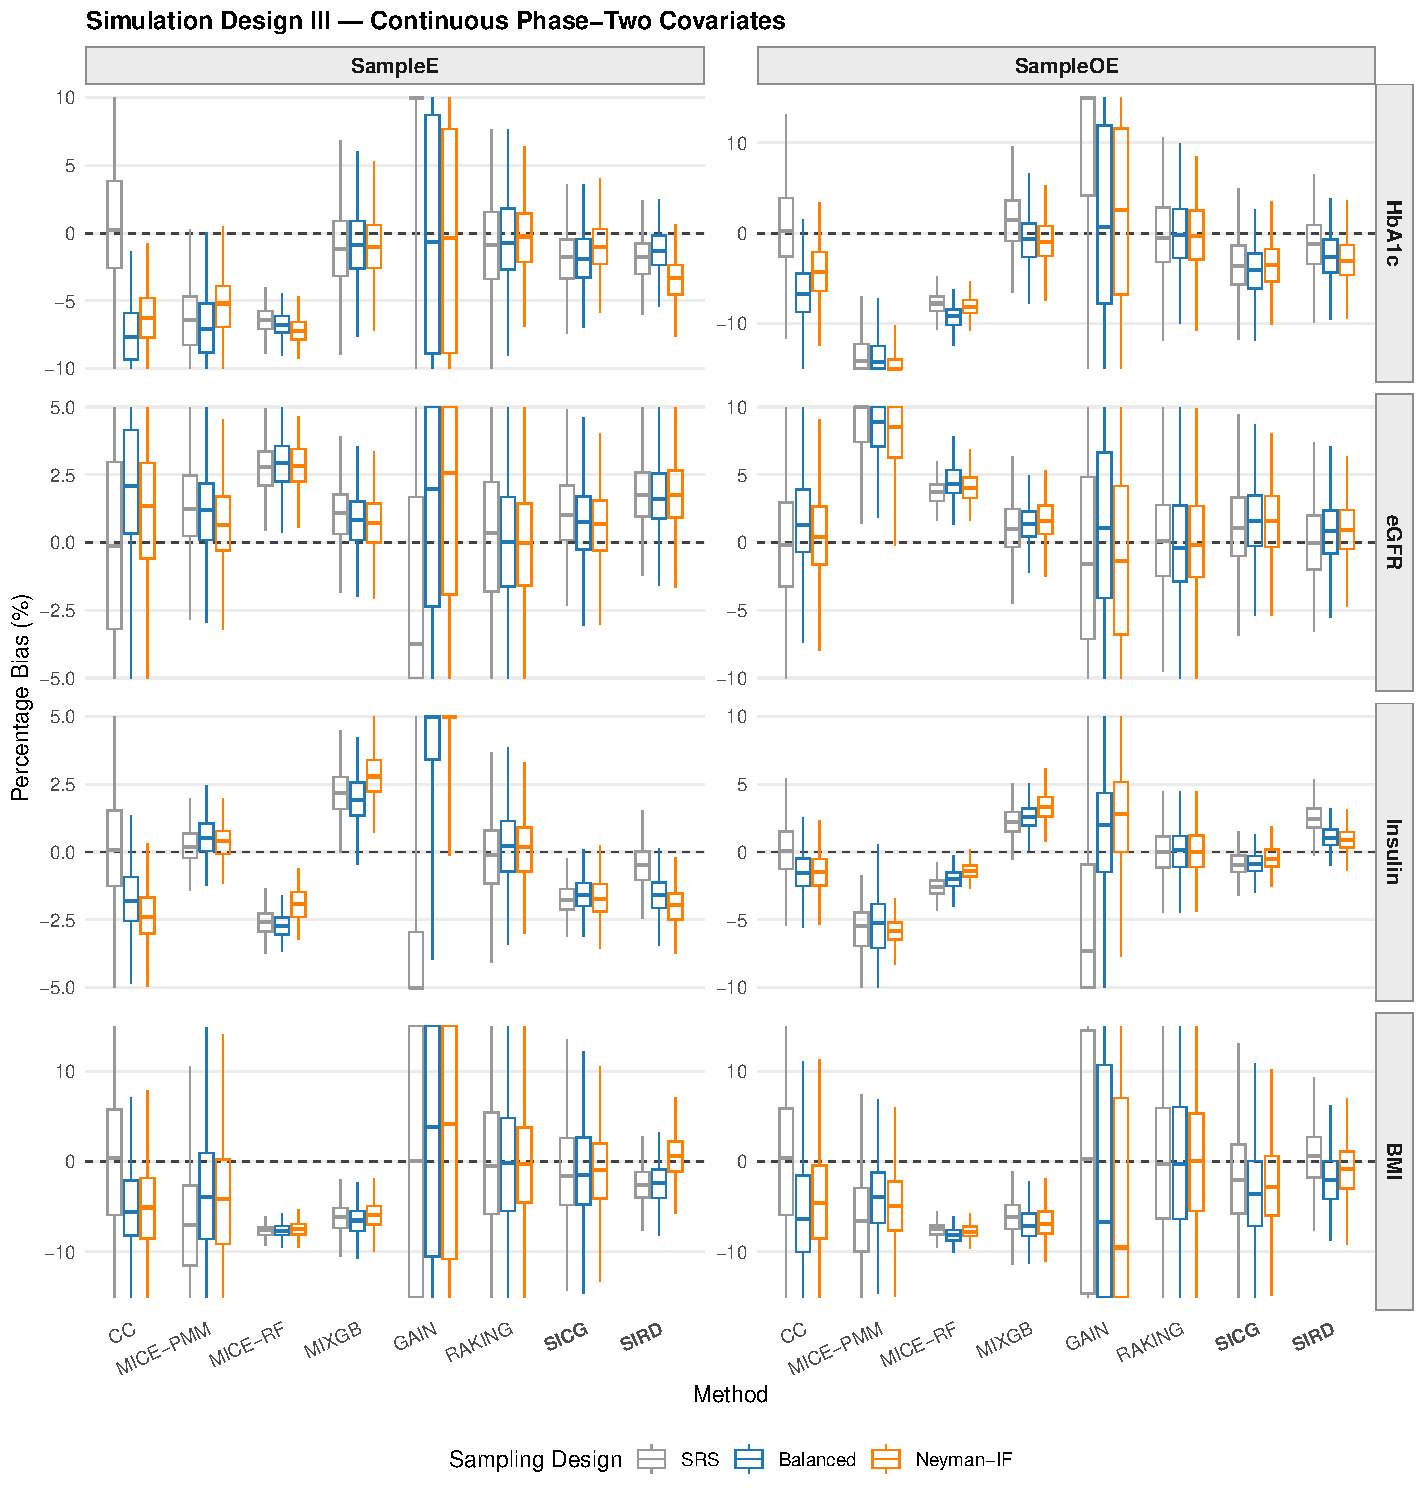
\includegraphics[width=\linewidth,height=0.86\textheight,keepaspectratio]{surv_continuous_phase2_pctbias.pdf}
\caption{Per-replicate percentage bias of the continuous Phase-Two (validated, error-prone) covariates, Simulation Design~III, under \texttt{SampleE} and \texttt{SampleOE}.}
\label{fig:appc_simII_cont}
\end{figure}
\end{landscape}
\clearpage

\begin{landscape}
\begin{figure}[p]
\centering
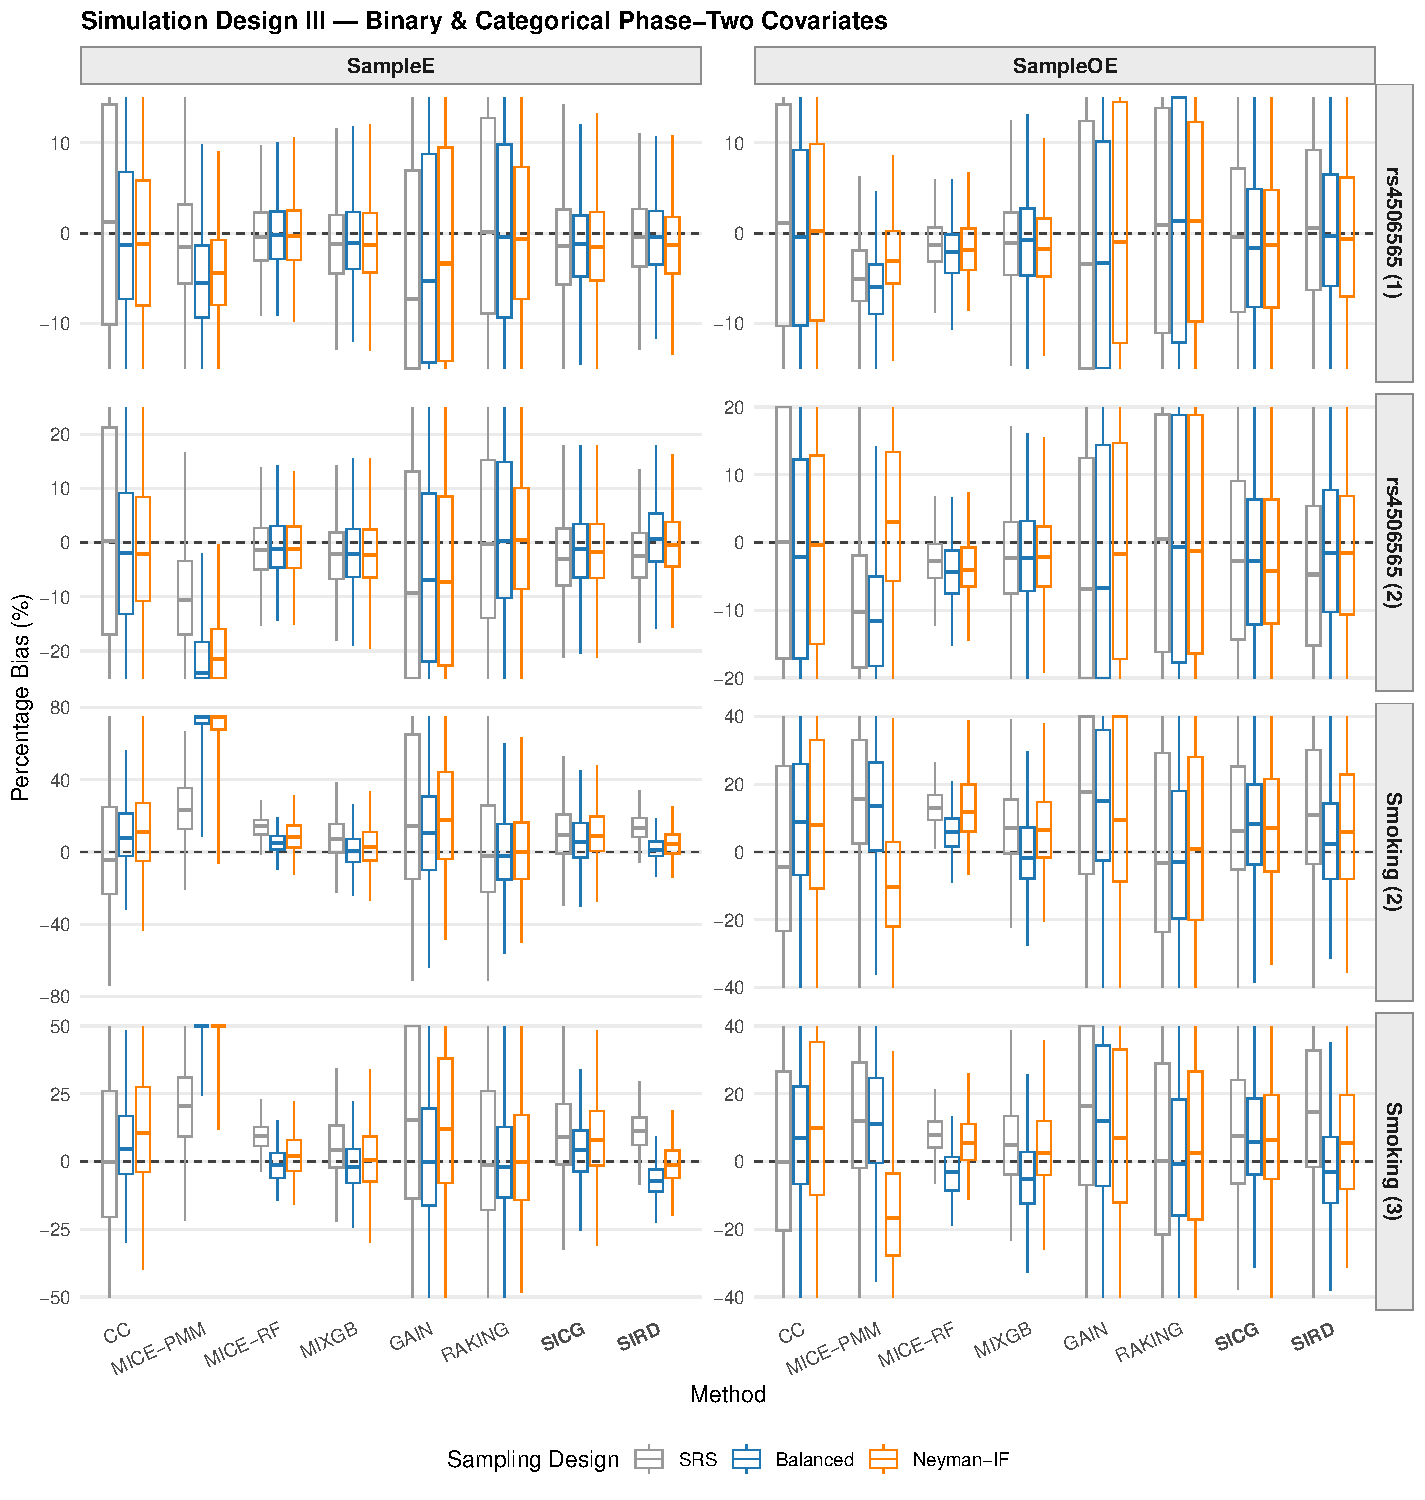
\includegraphics[width=\linewidth,height=0.86\textheight,keepaspectratio]{surv_categorical_phase2_pctbias.pdf}
\caption{Per-replicate percentage bias of the binary and categorical Phase-Two covariates, Simulation Design~III.}
\label{fig:appc_simII_cat}
\end{figure}
\end{landscape}
\clearpage

\begin{landscape}
\begin{figure}[p]
\centering
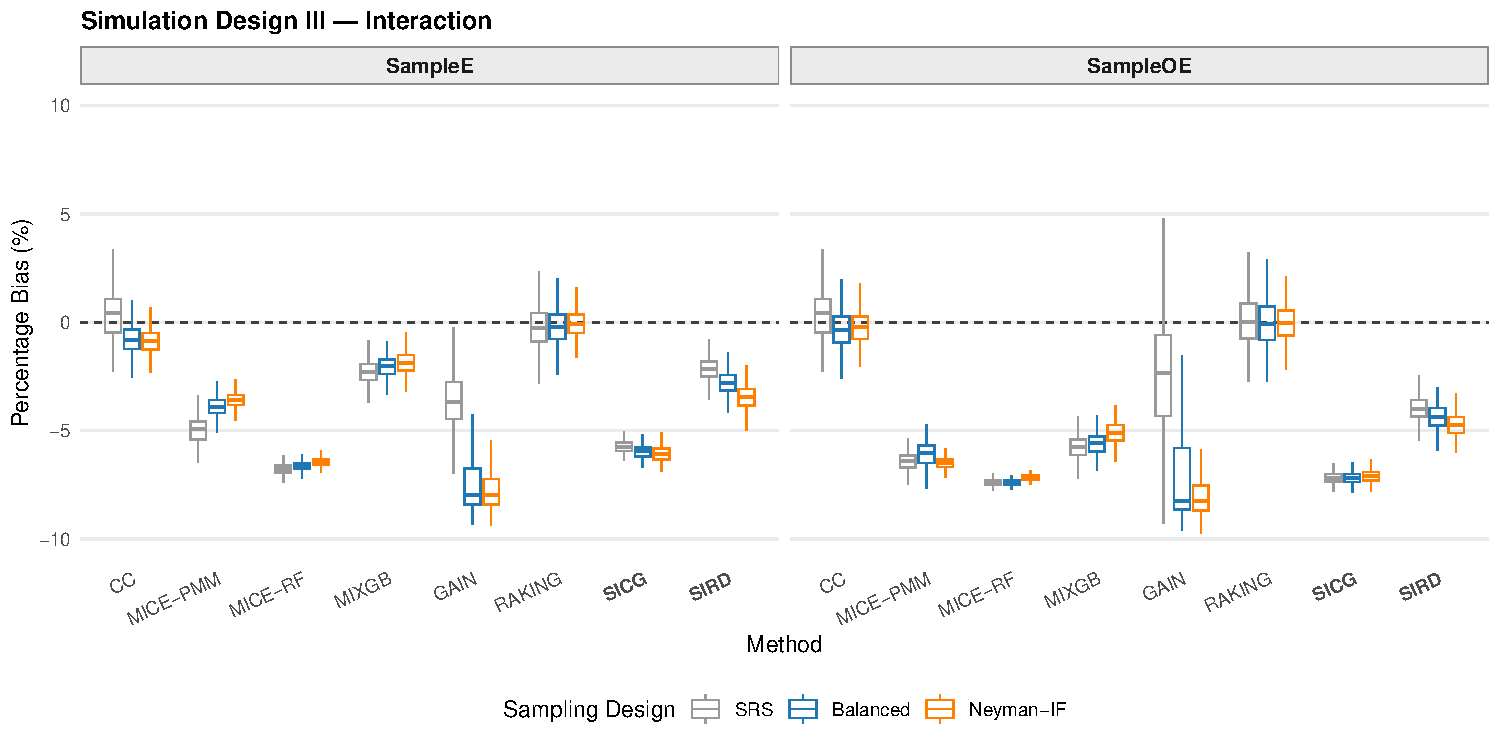
\includegraphics[width=\linewidth,height=0.86\textheight,keepaspectratio]{surv_interaction_pctbias.pdf}
\caption{Per-replicate percentage bias of the interaction, Simulation Design~III.}
\label{fig:appc_simII_inter}
\end{figure}
\end{landscape}
\clearpage

\begin{figure}[p]
\centering
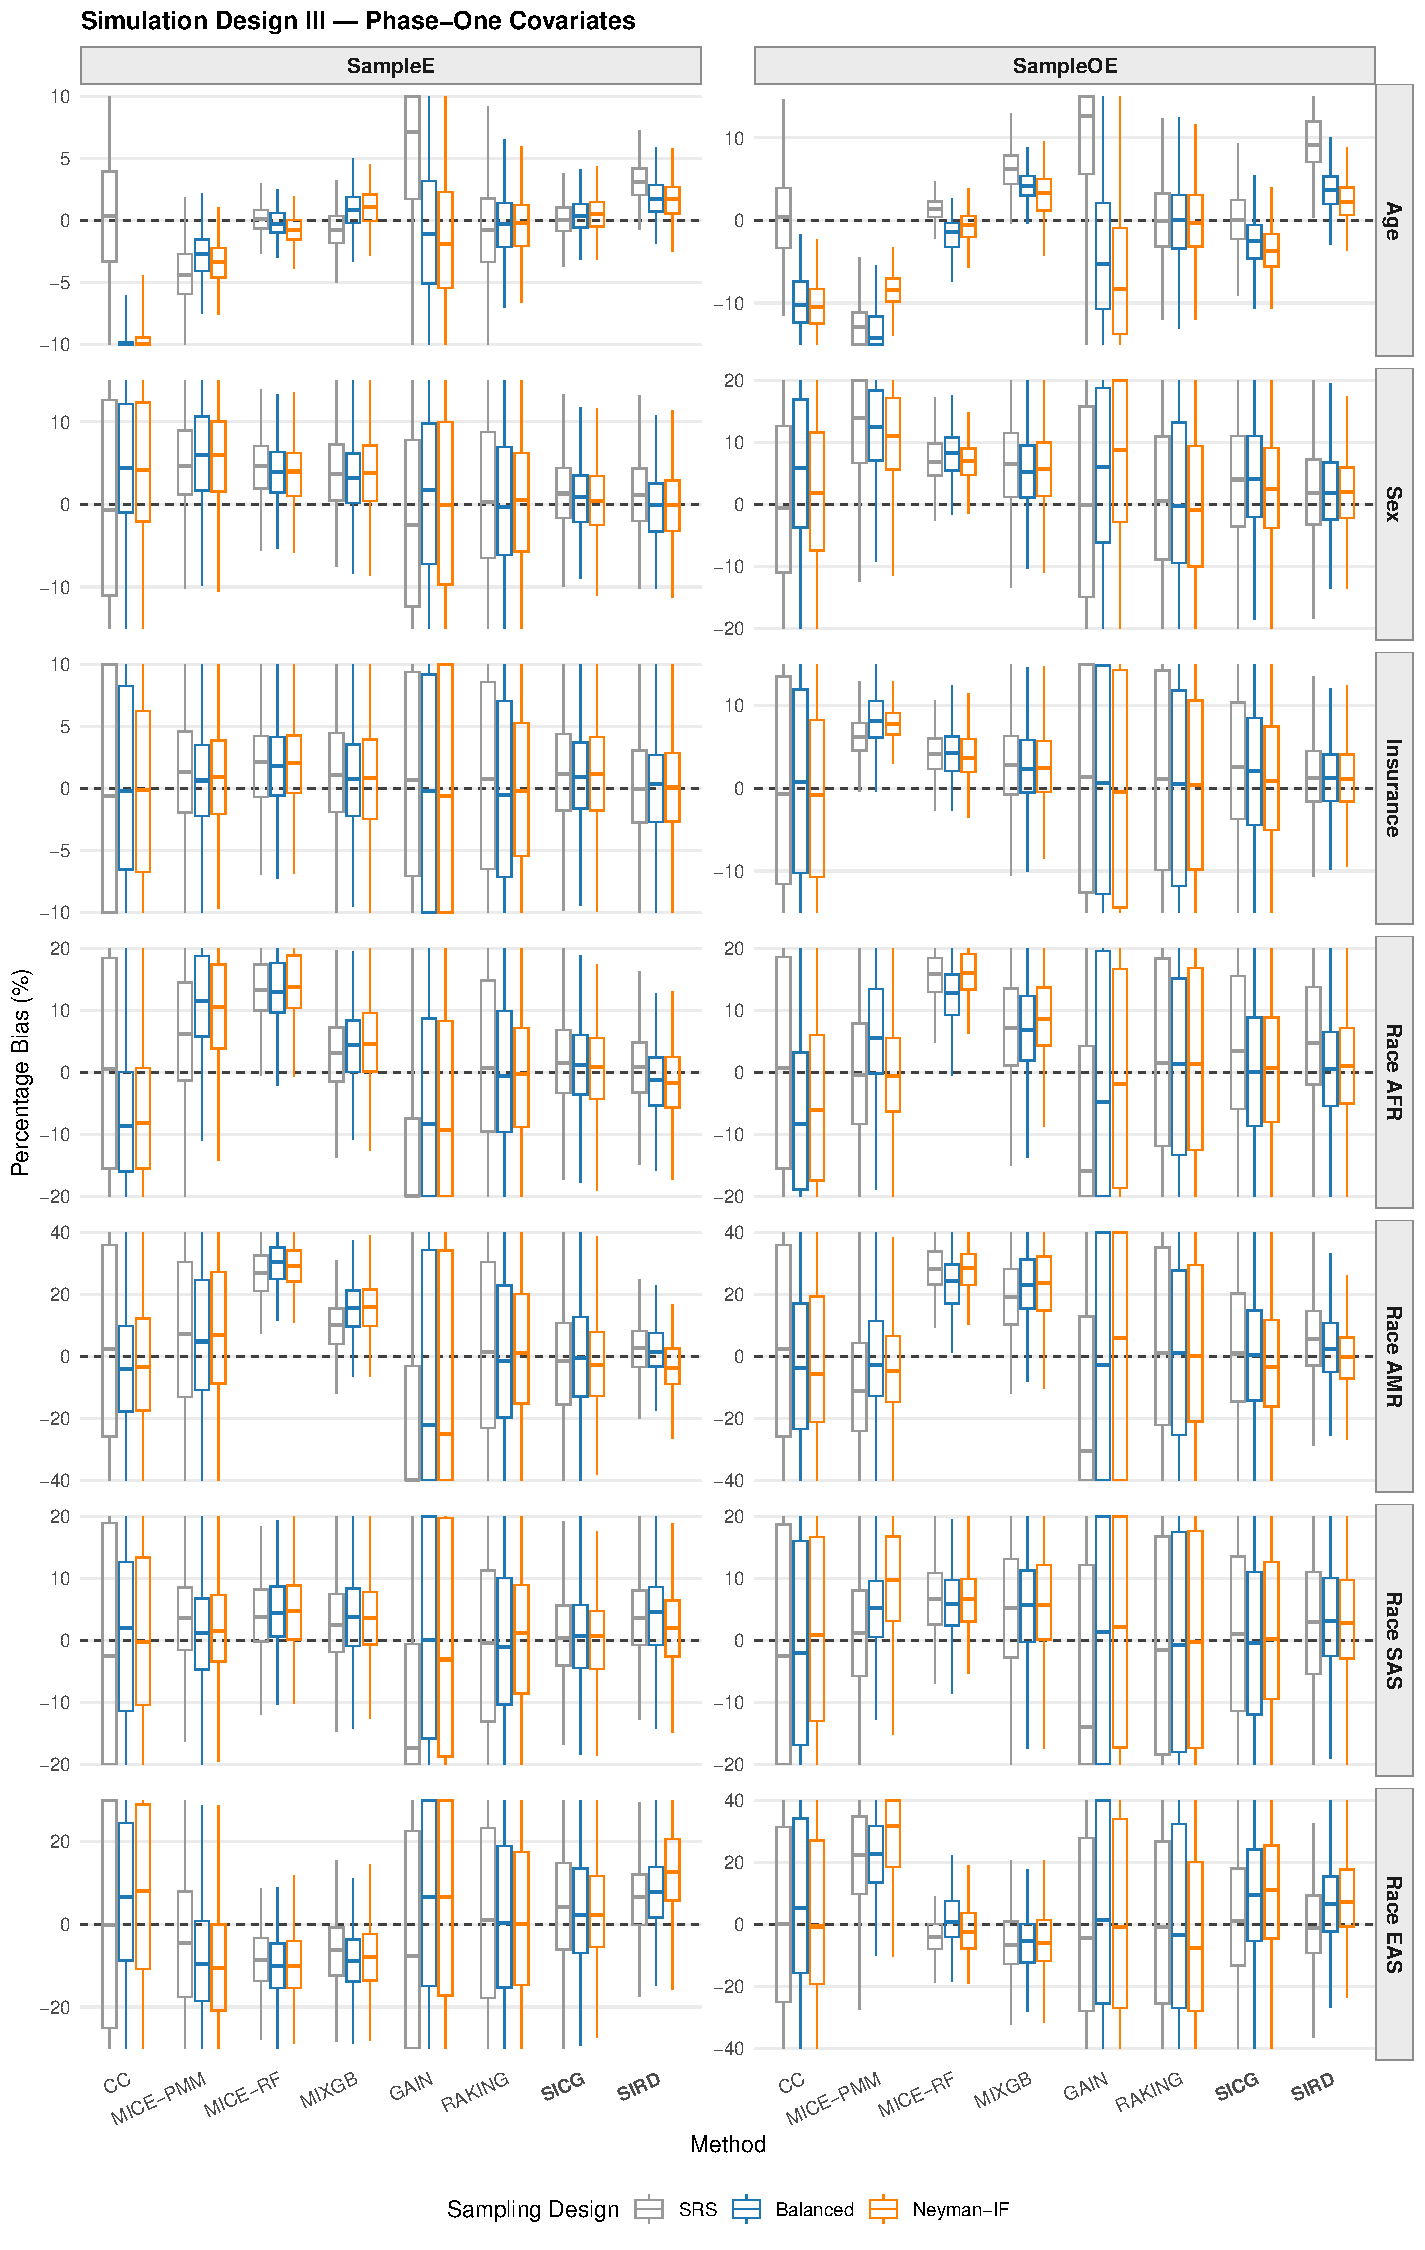
\includegraphics[width=\linewidth,height=0.9\textheight,keepaspectratio]{surv_phase1cov_pctbias.pdf}
\caption{Per-replicate percentage bias of the Phase-One (fully observed) covariates, Simulation Design~III.}
\label{fig:appc_simII_p1}
\end{figure}
\clearpage

\begin{figure}[p]
\centering
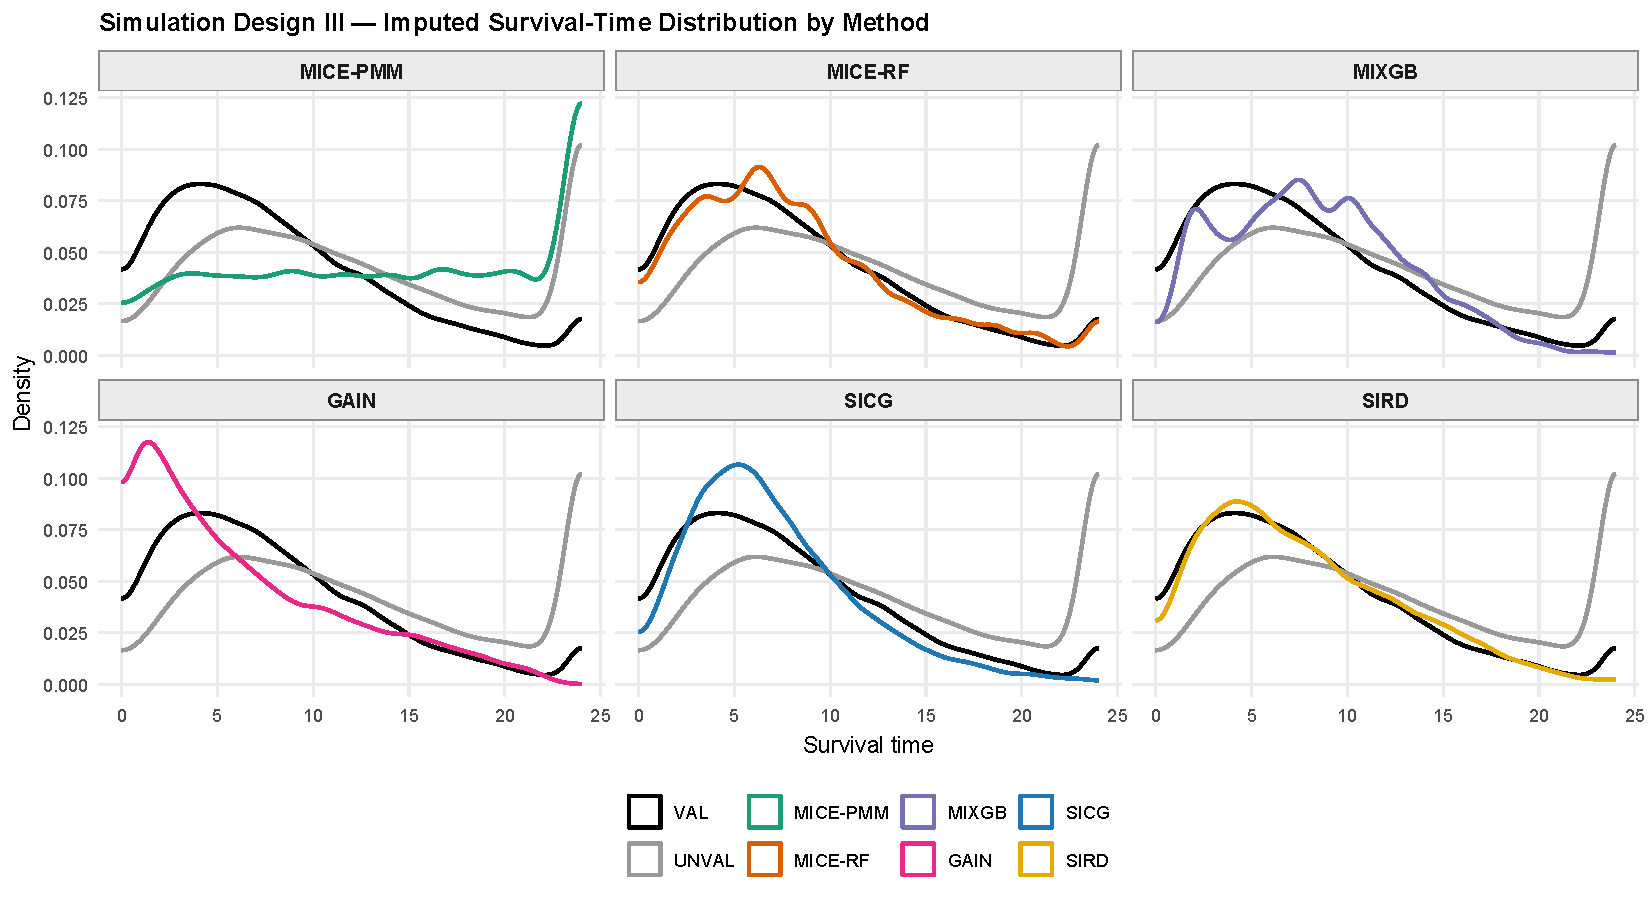
\includegraphics[width=\linewidth]{simIII_TI_density.pdf}
\caption{Imputed survival-time distribution under Simulation Design~III with outcome error (\texttt{SampleOE}), simple random sampling, for the first imputation of a single replicate and restricted to the unvalidated units. In each panel the true survival time is drawn in black, the error-prone observed time in grey, and the named method's imputed survival time in colour. The true distribution is right-skewed with a pile-up at the administrative censoring bound. SIRD and MICE-RF stay closest to it; SICG is too concentrated near the mode; GAIN shifts the mode to shorter times; MIXGB adds spurious secondary modes; MICE-PMM flattens the body and exaggerates the censoring spike.}
\label{fig:appc_simIII_TIdensity}
\end{figure}

\FloatBarrier

\clearpage
\section{The VCCC case study}
\label{app:suppC_vccc}

This section collects the full supplementary results for the VCCC case study, an outpatient cohort of patients living with HIV for which paired validated and error-prone records are available. Results are reported for the Gaussian, Binomial and Cox analysis models in turn, by coefficient group, separating the imputed Phase-Two covariates from the fully observed Phase-One covariates; the full per-design metric tables appear first, followed by the per-replicate percentage-bias figures.

\subsection{Full per-design metrics}

\begin{landscape}
\definecolor{rankone}{RGB}{33,113,181}\definecolor{ranktwo}{RGB}{107,174,214}\definecolor{rankthree}{RGB}{198,219,239}
\footnotesize\setlength{\tabcolsep}{3.5pt}
\begin{longtable}{llrrrrrrrrrr}
\caption{Full repeated-validation-subsampling metrics for the VCCC Gaussian model over all sampling designs. Metrics, aggregation and shading are as in Table~\ref{tab:appc_nutri_Gaussian}. The only covariate assigned to the Continuous Phase-One Covariates block is the year of enrolment, which enters only the Binomial and Cox models, so this block is empty for the Gaussian model.}
\label{tab:appc_vccc_LM} \\
\toprule
Design & Metric & \multicolumn{1}{c}{CC} & \multicolumn{1}{c}{UNVAL} & \multicolumn{1}{c}{MICE-PMM} & \multicolumn{1}{c}{MICE-RF} & \multicolumn{1}{c}{MIXGB} & \multicolumn{1}{c}{TabCSDI} & \multicolumn{1}{c}{GAIN} & \multicolumn{1}{c}{RAKING} & \multicolumn{1}{c}{\textbf{SICG}} & \multicolumn{1}{c}{\textbf{SIRD}} \\
\midrule
\endfirsthead
\multicolumn{12}{l}{\footnotesize\itshape Table~\ref{tab:appc_vccc_LM} (continued)} \\
\toprule
Design & Metric & \multicolumn{1}{c}{CC} & \multicolumn{1}{c}{UNVAL} & \multicolumn{1}{c}{MICE-PMM} & \multicolumn{1}{c}{MICE-RF} & \multicolumn{1}{c}{MIXGB} & \multicolumn{1}{c}{TabCSDI} & \multicolumn{1}{c}{GAIN} & \multicolumn{1}{c}{RAKING} & \multicolumn{1}{c}{\textbf{SICG}} & \multicolumn{1}{c}{\textbf{SIRD}} \\
\midrule
\endhead
\midrule \multicolumn{12}{r}{\footnotesize\itshape continued on next page} \\
\endfoot
\bottomrule
\endlastfoot
\multicolumn{12}{l}{\textbf{Continuous Phase-Two Covariates}} \\
\addlinespace[2pt]
\quad \texttt{SRS} & Mean $|$Bias$|$ (\%) & \cellcolor{ranktwo}1.1 & 4.1 & 14.5 & 12.0 & 7.1 & 5.2 & 3.5 & \cellcolor{rankone}0.2 & 2.9 & \cellcolor{rankthree}2.5 \\
 & Rel.\ RMSE (\%) & 19.1 & \cellcolor{ranktwo}4.1 & 22.0 & 12.7 & 8.9 & 9.6 & 12.1 & \cellcolor{rankone}4.0 & \cellcolor{rankthree}4.8 & \cellcolor{ranktwo}4.1 \\
 & Emp.\ SE & 0.048 &  & 0.038 & 0.013 & 0.020 & 0.031 & 0.042 & 0.017 & 0.013 & 0.012 \\
 & Mean SE & 0.052 & 0.023 & 0.027 & 0.028 & 0.032 & 0.031 & 0.026 & 0.029 & 0.026 & 0.027 \\
 & SE ratio & \cellcolor{ranktwo}1.08 &  & \cellcolor{rankthree}0.71 & 2.15 & 1.60 & \cellcolor{rankone}1.00 & 0.62 & 1.71 & 2.00 & 2.25 \\
 & Nom.\ Cov. & \cellcolor{rankone}0.97 & \cellcolor{rankthree}1.00 & 0.54 & 0.74 & \cellcolor{ranktwo}0.98 & 0.59 & 0.84 & \cellcolor{rankthree}1.00 & \cellcolor{rankthree}1.00 & \cellcolor{rankthree}1.00 \\
 & Orc.\ Cov.\ (Emp) & \cellcolor{rankone}0.95 &  & 0.59 & 0.18 & 0.46 & 0.46 & \cellcolor{ranktwo}0.94 & \cellcolor{ranktwo}0.96 & \cellcolor{rankthree}0.85 & 0.83 \\
 & Orc.\ Cov.\ (BC) & \cellcolor{ranktwo}0.97 & \cellcolor{rankthree}1.00 & 0.81 & \cellcolor{rankthree}1.00 & \cellcolor{rankthree}1.00 & \cellcolor{rankone}0.96 & 0.89 & \cellcolor{rankthree}1.00 & \cellcolor{rankthree}1.00 & \cellcolor{rankthree}1.00 \\
\addlinespace[2pt]
\quad \texttt{RS} & Mean $|$Bias$|$ (\%) & 13.8 & 4.1 & 2.9 & 8.4 & 4.2 & 5.5 & \cellcolor{rankthree}2.3 & \cellcolor{rankone}0.7 & \cellcolor{rankone}0.7 & \cellcolor{ranktwo}1.0 \\
 & Rel.\ RMSE (\%) & 13.8 & \cellcolor{rankthree}4.1 & 5.8 & 8.5 & 5.7 & 7.8 & 7.3 & \cellcolor{rankone}0.7 & \cellcolor{ranktwo}1.1 & \cellcolor{ranktwo}1.1 \\
 & Emp.\ SE & 0.000 &  & 0.002 & 0.002 & 0.007 & 0.014 & 0.023 & 0.000 & 0.002 & 0.002 \\
 & Mean SE & 0.091 & 0.023 & 0.025 & 0.025 & 0.030 & 0.027 & 0.026 & 0.052 & 0.024 & 0.025 \\
 & SE ratio &  &  & 12.50 & 12.50 & \cellcolor{rankthree}4.29 & \cellcolor{ranktwo}1.93 & \cellcolor{rankone}1.13 &  & 12.00 & 12.50 \\
 & Nom.\ Cov. & \cellcolor{ranktwo}1.00 & \cellcolor{ranktwo}1.00 & 0.48 & \cellcolor{ranktwo}1.00 & \cellcolor{ranktwo}1.00 & \cellcolor{rankthree}0.66 & \cellcolor{rankone}0.97 & \cellcolor{ranktwo}1.00 & \cellcolor{ranktwo}1.00 & \cellcolor{ranktwo}1.00 \\
 & Orc.\ Cov.\ (Emp) & 0.00 &  & 0.32 & 0.00 & 0.31 & 0.32 & \cellcolor{rankone}0.96 & 0.00 & \cellcolor{ranktwo}0.84 & \cellcolor{rankthree}0.45 \\
 & Orc.\ Cov.\ (BC) & \cellcolor{ranktwo}1.00 & \cellcolor{ranktwo}1.00 & \cellcolor{ranktwo}1.00 & \cellcolor{ranktwo}1.00 & \cellcolor{ranktwo}1.00 & \cellcolor{ranktwo}1.00 & \cellcolor{rankone}0.97 & \cellcolor{ranktwo}1.00 & \cellcolor{ranktwo}1.00 & \cellcolor{ranktwo}1.00 \\
\addlinespace[2pt]
\quad \texttt{WRS} & Mean $|$Bias$|$ (\%) & 55.1 & 4.1 & \cellcolor{ranktwo}1.3 & 5.8 & 8.4 & 4.8 & 5.9 & \cellcolor{ranktwo}1.3 & \cellcolor{rankthree}3.2 & \cellcolor{rankone}0.7 \\
 & Rel.\ RMSE (\%) & 56.4 & 4.1 & 6.8 & 6.2 & 9.0 & 6.6 & 9.8 & \cellcolor{ranktwo}1.8 & \cellcolor{rankthree}3.5 & \cellcolor{rankone}1.2 \\
 & Emp.\ SE & 0.014 &  & 0.010 & 0.005 & 0.012 & 0.021 & 0.024 & 0.003 & 0.004 & 0.003 \\
 & Mean SE & 0.088 & 0.023 & 0.025 & 0.025 & 0.034 & 0.026 & 0.025 & 0.062 & 0.025 & 0.024 \\
 & SE ratio & 6.29 &  & \cellcolor{rankthree}2.50 & 5.00 & 2.83 & \cellcolor{ranktwo}1.24 & \cellcolor{rankone}1.04 & 20.67 & 6.25 & 8.00 \\
 & Nom.\ Cov. & 0.33 & \cellcolor{rankthree}1.00 & \cellcolor{ranktwo}0.99 & \cellcolor{rankthree}1.00 & \cellcolor{rankthree}1.00 & \cellcolor{rankone}0.93 & 0.85 & \cellcolor{rankthree}1.00 & \cellcolor{rankthree}1.00 & \cellcolor{rankthree}1.00 \\
 & Orc.\ Cov.\ (Emp) & 0.08 &  & 0.60 & 0.20 & 0.26 & \cellcolor{rankthree}0.64 & \cellcolor{rankone}0.86 & 0.52 & 0.35 & \cellcolor{ranktwo}0.79 \\
 & Orc.\ Cov.\ (BC) & \cellcolor{rankthree}1.00 & \cellcolor{rankthree}1.00 & \cellcolor{rankthree}1.00 & \cellcolor{rankthree}1.00 & \cellcolor{rankthree}1.00 & \cellcolor{ranktwo}0.98 & \cellcolor{rankone}0.97 & \cellcolor{rankthree}1.00 & \cellcolor{rankthree}1.00 & \cellcolor{rankthree}1.00 \\
\addlinespace[2pt]
\quad \texttt{SFS} & Mean $|$Bias$|$ (\%) & 58.1 & 4.1 & 7.9 & \cellcolor{ranktwo}1.7 & 9.6 & 3.3 & 6.4 & \cellcolor{rankthree}2.1 & 5.3 & \cellcolor{rankone}0.8 \\
 & Rel.\ RMSE (\%) & 58.1 & 4.1 & 8.0 & \cellcolor{rankthree}2.4 & 9.9 & 6.4 & 10.2 & \cellcolor{ranktwo}2.1 & 5.4 & \cellcolor{rankone}1.0 \\
 & Emp.\ SE & 0.000 &  & 0.003 & 0.003 & 0.011 & 0.024 & 0.026 & 0.000 & 0.003 & 0.002 \\
 & Mean SE & 0.104 & 0.023 & 0.029 & 0.029 & 0.037 & 0.032 & 0.026 & 0.083 & 0.026 & 0.024 \\
 & SE ratio &  &  & 9.67 & 9.67 & \cellcolor{rankthree}3.36 & \cellcolor{ranktwo}1.33 & \cellcolor{rankone}1.00 &  & 8.67 & 12.00 \\
 & Nom.\ Cov. & 0.33 & \cellcolor{ranktwo}1.00 & 0.67 & \cellcolor{ranktwo}1.00 & \cellcolor{ranktwo}1.00 & \cellcolor{rankone}0.96 & \cellcolor{rankthree}0.84 & \cellcolor{ranktwo}1.00 & \cellcolor{ranktwo}1.00 & \cellcolor{ranktwo}1.00 \\
 & Orc.\ Cov.\ (Emp) & 0.00 &  & 0.00 & \cellcolor{rankthree}0.56 & 0.04 & \cellcolor{ranktwo}0.63 & \cellcolor{rankone}0.86 & 0.00 & 0.03 & 0.53 \\
 & Orc.\ Cov.\ (BC) & \cellcolor{rankthree}1.00 & \cellcolor{rankthree}1.00 & \cellcolor{rankthree}1.00 & \cellcolor{rankthree}1.00 & \cellcolor{rankthree}1.00 & \cellcolor{ranktwo}0.98 & \cellcolor{rankone}0.97 & \cellcolor{rankthree}1.00 & \cellcolor{rankthree}1.00 & \cellcolor{rankthree}1.00 \\
\addlinespace[2pt]
\quad \texttt{ODS-Tail} & Mean $|$Bias$|$ (\%) & 10.4 & 4.1 & 6.9 & 15.2 & 13.0 & 10.9 & \cellcolor{rankthree}3.7 & 8.9 & \cellcolor{ranktwo}1.8 & \cellcolor{rankone}1.3 \\
 & Rel.\ RMSE (\%) & 10.4 & \cellcolor{rankthree}4.1 & 7.2 & 15.3 & 13.2 & 12.1 & 13.5 & 8.9 & \cellcolor{ranktwo}2.3 & \cellcolor{rankone}1.9 \\
 & Emp.\ SE & 0.000 &  & 0.003 & 0.003 & 0.010 & 0.019 & 0.045 & 0.000 & 0.003 & 0.003 \\
 & Mean SE & 0.057 & 0.023 & 0.024 & 0.026 & 0.033 & 0.027 & 0.027 & 0.098 & 0.025 & 0.027 \\
 & SE ratio &  &  & 8.00 & 8.67 & \cellcolor{rankthree}3.30 & \cellcolor{ranktwo}1.42 & \cellcolor{rankone}0.60 &  & 8.33 & 9.00 \\
 & Nom.\ Cov. & 0.67 & \cellcolor{ranktwo}1.00 & 0.67 & 0.67 & \cellcolor{rankone}0.99 & 0.39 & \cellcolor{rankthree}0.82 & \cellcolor{ranktwo}1.00 & \cellcolor{ranktwo}1.00 & \cellcolor{ranktwo}1.00 \\
 & Orc.\ Cov.\ (Emp) & 0.00 &  & 0.18 & 0.00 & 0.01 & \cellcolor{rankthree}0.28 & \cellcolor{rankone}0.94 & 0.00 & \cellcolor{ranktwo}0.49 & \cellcolor{ranktwo}0.49 \\
 & Orc.\ Cov.\ (BC) & \cellcolor{ranktwo}1.00 & \cellcolor{ranktwo}1.00 & \cellcolor{ranktwo}1.00 & \cellcolor{ranktwo}1.00 & \cellcolor{ranktwo}1.00 & \cellcolor{rankone}0.98 & \cellcolor{rankthree}0.87 & \cellcolor{ranktwo}1.00 & \cellcolor{ranktwo}1.00 & \cellcolor{ranktwo}1.00 \\
\addlinespace[2pt]
\quad \texttt{Neyman-ODS} & Mean $|$Bias$|$ (\%) & \cellcolor{rankthree}2.9 & 4.1 & 17.8 & 11.5 & 7.5 & 8.1 & 4.1 & \cellcolor{rankone}0.1 & 3.3 & \cellcolor{ranktwo}2.8 \\
 & Rel.\ RMSE (\%) & 20.2 & \cellcolor{ranktwo}4.1 & 20.7 & 12.4 & 9.4 & 11.4 & 12.4 & \cellcolor{rankone}3.9 & 5.0 & \cellcolor{rankthree}4.3 \\
 & Emp.\ SE & 0.048 &  & 0.027 & 0.014 & 0.021 & 0.031 & 0.042 & 0.017 & 0.013 & 0.012 \\
 & Mean SE & 0.052 & 0.023 & 0.031 & 0.028 & 0.031 & 0.030 & 0.026 & 0.029 & 0.026 & 0.026 \\
 & SE ratio & \cellcolor{ranktwo}1.08 &  & \cellcolor{rankthree}1.15 & 2.00 & 1.48 & \cellcolor{rankone}0.97 & 0.62 & 1.71 & 2.00 & 2.17 \\
 & Nom.\ Cov. & \cellcolor{rankone}0.96 & \cellcolor{rankthree}1.00 & 0.63 & 0.74 & \cellcolor{ranktwo}0.98 & 0.47 & 0.84 & \cellcolor{rankthree}1.00 & \cellcolor{rankthree}1.00 & \cellcolor{rankthree}1.00 \\
 & Orc.\ Cov.\ (Emp) & \cellcolor{ranktwo}0.93 &  & 0.31 & 0.22 & 0.46 & 0.39 & \cellcolor{ranktwo}0.93 & \cellcolor{rankone}0.95 & \cellcolor{rankthree}0.83 & 0.82 \\
 & Orc.\ Cov.\ (BC) & \cellcolor{ranktwo}0.97 & 1.00 & \cellcolor{rankthree}0.98 & 1.00 & 0.99 & \cellcolor{rankone}0.95 & 0.89 & 1.00 & 1.00 & 1.00 \\
\addlinespace[2pt]
\quad \texttt{Neyman-IF} & Mean $|$Bias$|$ (\%) & \cellcolor{ranktwo}1.6 & 4.1 & 18.2 & 11.7 & 7.2 & 7.9 & 4.3 & \cellcolor{rankone}0.2 & 1.8 & \cellcolor{rankthree}1.7 \\
 & Rel.\ RMSE (\%) & 19.8 & \cellcolor{rankthree}4.1 & 21.2 & 12.5 & 9.3 & 10.7 & 13.7 & \cellcolor{rankone}3.9 & 5.2 & \cellcolor{ranktwo}4.0 \\
 & Emp.\ SE & 0.047 &  & 0.028 & 0.014 & 0.021 & 0.029 & 0.049 & 0.017 & 0.017 & 0.014 \\
 & Mean SE & 0.052 & 0.023 & 0.031 & 0.028 & 0.031 & 0.030 & 0.026 & 0.029 & 0.026 & 0.027 \\
 & SE ratio & \cellcolor{ranktwo}1.11 &  & \cellcolor{ranktwo}1.11 & 2.00 & 1.48 & \cellcolor{rankone}1.03 & \cellcolor{rankthree}0.53 & 1.71 & 1.53 & 1.93 \\
 & Nom.\ Cov. & \cellcolor{rankone}0.96 & 1.00 & 0.62 & 0.73 & \cellcolor{ranktwo}0.97 & 0.50 & 0.81 & 1.00 & \cellcolor{rankthree}0.99 & 1.00 \\
 & Orc.\ Cov.\ (Emp) & \cellcolor{ranktwo}0.94 &  & 0.31 & 0.20 & 0.46 & 0.35 & \cellcolor{rankthree}0.93 & \cellcolor{rankone}0.95 & 0.90 & \cellcolor{ranktwo}0.94 \\
 & Orc.\ Cov.\ (BC) & \cellcolor{rankone}0.97 & \cellcolor{rankthree}1.00 & \cellcolor{rankone}0.97 & \cellcolor{rankthree}1.00 & \cellcolor{ranktwo}0.99 & \cellcolor{rankone}0.97 & 0.85 & \cellcolor{rankthree}1.00 & \cellcolor{ranktwo}0.99 & \cellcolor{rankthree}1.00 \\
\addlinespace[2pt]
\multicolumn{12}{l}{\textbf{Binary \& Categorical Phase-One Covariates}} \\
\addlinespace[2pt]
\quad \texttt{SRS} & Mean $|$Bias$|$ (\%) & \cellcolor{ranktwo}1.0 & 4.6 & 4.6 & 10.5 & 8.0 & 17.1 & \cellcolor{rankthree}1.3 & \cellcolor{rankone}0.0 & 1.6 & 2.3 \\
 & Rel.\ RMSE (\%) & 68.2 & \cellcolor{ranktwo}4.6 & 16.9 & 10.8 & 8.8 & 17.3 & 14.6 & \cellcolor{rankthree}6.1 & \cellcolor{rankone}4.5 & \cellcolor{ranktwo}4.6 \\
 & Emp.\ SE & 0.514 &  & 0.123 & 0.019 & 0.028 & 0.020 & 0.110 & 0.046 & 0.031 & 0.030 \\
 & Mean SE & 0.521 & 0.233 & 0.236 & 0.236 & 0.234 & 0.234 & 0.232 & 0.254 & 0.234 & 0.235 \\
 & SE ratio & \cellcolor{rankone}1.01 &  & \cellcolor{ranktwo}1.92 & 12.42 & 8.36 & 11.70 & \cellcolor{rankthree}2.11 & 5.52 & 7.55 & 7.83 \\
 & Nom.\ Cov. & \cellcolor{rankone}0.95 & \cellcolor{rankthree}1.00 & \cellcolor{ranktwo}0.99 & \cellcolor{rankthree}1.00 & \cellcolor{rankthree}1.00 & \cellcolor{rankthree}1.00 & \cellcolor{ranktwo}0.99 & \cellcolor{rankthree}1.00 & \cellcolor{rankthree}1.00 & \cellcolor{rankthree}1.00 \\
 & Orc.\ Cov.\ (Emp) & \cellcolor{rankone}0.95 &  & \cellcolor{rankone}0.95 & 0.01 & 0.44 & 0.00 & \cellcolor{rankone}0.95 & \cellcolor{ranktwo}0.96 & \cellcolor{ranktwo}0.94 & \cellcolor{rankthree}0.93 \\
 & Orc.\ Cov.\ (BC) & \cellcolor{rankone}0.95 & \cellcolor{rankthree}1.00 & \cellcolor{ranktwo}0.99 & \cellcolor{rankthree}1.00 & \cellcolor{rankthree}1.00 & \cellcolor{rankthree}1.00 & \cellcolor{ranktwo}0.99 & \cellcolor{rankthree}1.00 & \cellcolor{rankthree}1.00 & \cellcolor{rankthree}1.00 \\
\addlinespace[2pt]
\quad \texttt{RS} & Mean $|$Bias$|$ (\%) & 22.1 & 4.6 & 13.1 & 7.6 & 7.5 & 18.1 & \cellcolor{ranktwo}0.8 & 1.6 & \cellcolor{rankthree}1.1 & \cellcolor{rankone}0.1 \\
 & Rel.\ RMSE (\%) & 22.1 & 4.6 & 13.1 & 7.7 & 7.8 & 18.1 & 9.9 & \cellcolor{rankthree}1.6 & \cellcolor{ranktwo}1.5 & \cellcolor{rankone}0.7 \\
 & Emp.\ SE & 0.000 &  & 0.005 & 0.005 & 0.017 & 0.007 & 0.075 & 0.000 & 0.008 & 0.005 \\
 & Mean SE & 0.891 & 0.233 & 0.234 & 0.235 & 0.234 & 0.234 & 0.233 & 0.409 & 0.233 & 0.234 \\
 & SE ratio &  &  & 46.80 & 47.00 & \cellcolor{ranktwo}13.76 & 33.43 & \cellcolor{rankone}3.11 &  & \cellcolor{rankthree}29.12 & 46.80 \\
 & Nom.\ Cov. & \cellcolor{rankone}1.00 & \cellcolor{rankone}1.00 & \cellcolor{rankone}1.00 & \cellcolor{rankone}1.00 & \cellcolor{rankone}1.00 & \cellcolor{rankone}1.00 & \cellcolor{rankone}1.00 & \cellcolor{rankone}1.00 & \cellcolor{rankone}1.00 & \cellcolor{rankone}1.00 \\
 & Orc.\ Cov.\ (Emp) & 0.00 &  & 0.00 & 0.00 & 0.09 & 0.00 & \cellcolor{ranktwo}0.94 & 0.00 & \cellcolor{rankthree}0.81 & \cellcolor{rankone}0.95 \\
 & Orc.\ Cov.\ (BC) & \cellcolor{rankone}1.00 & \cellcolor{rankone}1.00 & \cellcolor{rankone}1.00 & \cellcolor{rankone}1.00 & \cellcolor{rankone}1.00 & \cellcolor{rankone}1.00 & \cellcolor{rankone}1.00 & \cellcolor{rankone}1.00 & \cellcolor{rankone}1.00 & \cellcolor{rankone}1.00 \\
\addlinespace[2pt]
\quad \texttt{WRS} & Mean $|$Bias$|$ (\%) & 69.8 & 4.6 & 7.4 & 5.8 & 3.8 & 15.1 & \cellcolor{rankthree}3.0 & 3.5 & \cellcolor{ranktwo}2.2 & \cellcolor{rankone}1.8 \\
 & Rel.\ RMSE (\%) & 71.9 & 4.6 & 7.6 & 6.1 & 5.1 & 15.3 & 13.6 & \cellcolor{rankthree}3.9 & \cellcolor{ranktwo}2.8 & \cellcolor{rankone}2.3 \\
 & Emp.\ SE & 0.131 &  & 0.009 & 0.012 & 0.025 & 0.021 & 0.100 & 0.013 & 0.014 & 0.011 \\
 & Mean SE & 0.861 & 0.233 & 0.233 & 0.234 & 0.233 & 0.233 & 0.232 & 0.460 & 0.233 & 0.233 \\
 & SE ratio & \cellcolor{ranktwo}6.57 &  & 25.89 & 19.50 & \cellcolor{rankthree}9.32 & 11.10 & \cellcolor{rankone}2.32 & 35.38 & 16.64 & 21.18 \\
 & Nom.\ Cov. & \cellcolor{rankone}1.00 & \cellcolor{rankone}1.00 & \cellcolor{rankone}1.00 & \cellcolor{rankone}1.00 & \cellcolor{rankone}1.00 & \cellcolor{rankone}1.00 & \cellcolor{rankone}1.00 & \cellcolor{rankone}1.00 & \cellcolor{rankone}1.00 & \cellcolor{rankone}1.00 \\
 & Orc.\ Cov.\ (Emp) & 0.02 &  & 0.00 & 0.03 & \cellcolor{rankthree}0.82 & 0.02 & \cellcolor{rankone}0.96 & 0.45 & 0.79 & \cellcolor{ranktwo}0.84 \\
 & Orc.\ Cov.\ (BC) & \cellcolor{rankone}1.00 & \cellcolor{rankone}1.00 & \cellcolor{rankone}1.00 & \cellcolor{rankone}1.00 & \cellcolor{rankone}1.00 & \cellcolor{rankone}1.00 & \cellcolor{rankone}1.00 & \cellcolor{rankone}1.00 & \cellcolor{rankone}1.00 & \cellcolor{rankone}1.00 \\
\addlinespace[2pt]
\quad \texttt{SFS} & Mean $|$Bias$|$ (\%) & 56.2 & 4.6 & 11.3 & \cellcolor{rankthree}3.7 & \cellcolor{ranktwo}3.1 & 14.1 & 5.9 & 9.1 & 4.6 & \cellcolor{rankone}2.0 \\
 & Rel.\ RMSE (\%) & 56.2 & 4.6 & 11.3 & \cellcolor{ranktwo}3.8 & \cellcolor{rankthree}4.3 & 14.4 & 12.4 & 9.1 & 4.8 & \cellcolor{rankone}2.0 \\
 & Emp.\ SE & 0.000 &  & 0.005 & 0.007 & 0.022 & 0.021 & 0.082 & 0.000 & 0.010 & 0.004 \\
 & Mean SE & 0.883 & 0.233 & 0.233 & 0.235 & 0.233 & 0.233 & 0.232 & 0.465 & 0.233 & 0.234 \\
 & SE ratio &  &  & 46.60 & 33.57 & \cellcolor{ranktwo}10.59 & \cellcolor{rankthree}11.10 & \cellcolor{rankone}2.83 &  & 23.30 & 58.50 \\
 & Nom.\ Cov. & \cellcolor{rankone}1.00 & \cellcolor{rankone}1.00 & \cellcolor{rankone}1.00 & \cellcolor{rankone}1.00 & \cellcolor{rankone}1.00 & \cellcolor{rankone}1.00 & \cellcolor{rankone}1.00 & \cellcolor{rankone}1.00 & \cellcolor{rankone}1.00 & \cellcolor{rankone}1.00 \\
 & Orc.\ Cov.\ (Emp) & 0.00 &  & 0.00 & 0.01 & \cellcolor{ranktwo}0.80 & 0.04 & \cellcolor{rankone}0.91 & 0.00 & \cellcolor{rankthree}0.06 & \cellcolor{rankthree}0.06 \\
 & Orc.\ Cov.\ (BC) & \cellcolor{rankone}1.00 & \cellcolor{rankone}1.00 & \cellcolor{rankone}1.00 & \cellcolor{rankone}1.00 & \cellcolor{rankone}1.00 & \cellcolor{rankone}1.00 & \cellcolor{rankone}1.00 & \cellcolor{rankone}1.00 & \cellcolor{rankone}1.00 & \cellcolor{rankone}1.00 \\
\addlinespace[2pt]
\quad \texttt{ODS-Tail} & Mean $|$Bias$|$ (\%) & 74.9 & 4.6 & 20.9 & 14.7 & 11.4 & 19.9 & 6.2 & \cellcolor{ranktwo}1.8 & \cellcolor{rankthree}1.9 & \cellcolor{rankone}1.2 \\
 & Rel.\ RMSE (\%) & 74.9 & 4.6 & 20.9 & 14.8 & 11.5 & 19.9 & 15.6 & \cellcolor{ranktwo}1.8 & \cellcolor{rankthree}2.3 & \cellcolor{rankone}1.7 \\
 & Emp.\ SE & 0.000 &  & 0.005 & 0.005 & 0.014 & 0.012 & 0.108 & 0.000 & 0.010 & 0.009 \\
 & Mean SE & 0.617 & 0.233 & 0.235 & 0.236 & 0.235 & 0.234 & 0.232 & 0.827 & 0.234 & 0.236 \\
 & SE ratio &  &  & 47.00 & 47.20 & \cellcolor{ranktwo}16.79 & \cellcolor{rankthree}19.50 & \cellcolor{rankone}2.15 &  & 23.40 & 26.22 \\
 & Nom.\ Cov. & \cellcolor{rankone}1.00 & \cellcolor{rankone}1.00 & \cellcolor{rankone}1.00 & \cellcolor{rankone}1.00 & \cellcolor{rankone}1.00 & \cellcolor{rankone}1.00 & \cellcolor{rankone}1.00 & \cellcolor{rankone}1.00 & \cellcolor{rankone}1.00 & \cellcolor{rankone}1.00 \\
 & Orc.\ Cov.\ (Emp) & 0.00 &  & 0.00 & 0.00 & 0.00 & 0.00 & \cellcolor{rankone}0.95 & 0.00 & \cellcolor{rankthree}0.70 & \cellcolor{ranktwo}0.82 \\
 & Orc.\ Cov.\ (BC) & \cellcolor{rankone}1.00 & \cellcolor{rankone}1.00 & \cellcolor{rankone}1.00 & \cellcolor{rankone}1.00 & \cellcolor{rankone}1.00 & \cellcolor{rankone}1.00 & \cellcolor{rankone}1.00 & \cellcolor{rankone}1.00 & \cellcolor{rankone}1.00 & \cellcolor{rankone}1.00 \\
\addlinespace[2pt]
\quad \texttt{Neyman-ODS} & Mean $|$Bias$|$ (\%) & 3.9 & 4.6 & \cellcolor{rankthree}2.2 & 10.8 & 8.3 & 18.7 & \cellcolor{rankone}0.2 & \cellcolor{rankone}0.2 & \cellcolor{ranktwo}1.9 & 2.5 \\
 & Rel.\ RMSE (\%) & 72.2 & \cellcolor{rankone}4.6 & 11.7 & 11.2 & 9.2 & 18.8 & 14.0 & 6.1 & \cellcolor{rankthree}4.8 & \cellcolor{ranktwo}4.7 \\
 & Emp.\ SE & 0.544 &  & 0.087 & 0.021 & 0.029 & 0.017 & 0.106 & 0.046 & 0.033 & 0.030 \\
 & Mean SE & 0.532 & 0.233 & 0.237 & 0.236 & 0.234 & 0.234 & 0.232 & 0.255 & 0.234 & 0.235 \\
 & SE ratio & \cellcolor{rankone}0.98 &  & \cellcolor{rankthree}2.72 & 11.24 & 8.07 & 13.76 & \cellcolor{ranktwo}2.19 & 5.54 & 7.09 & 7.83 \\
 & Nom.\ Cov. & \cellcolor{rankone}0.94 & \cellcolor{ranktwo}1.00 & \cellcolor{ranktwo}1.00 & \cellcolor{ranktwo}1.00 & \cellcolor{ranktwo}1.00 & \cellcolor{ranktwo}1.00 & \cellcolor{ranktwo}1.00 & \cellcolor{ranktwo}1.00 & \cellcolor{ranktwo}1.00 & \cellcolor{ranktwo}1.00 \\
 & Orc.\ Cov.\ (Emp) & \cellcolor{ranktwo}0.94 &  & \cellcolor{rankthree}0.92 & 0.03 & 0.40 & 0.00 & \cellcolor{ranktwo}0.96 & \cellcolor{rankone}0.95 & \cellcolor{ranktwo}0.94 & 0.90 \\
 & Orc.\ Cov.\ (BC) & \cellcolor{rankone}0.94 & \cellcolor{ranktwo}1.00 & \cellcolor{ranktwo}1.00 & \cellcolor{ranktwo}1.00 & \cellcolor{ranktwo}1.00 & \cellcolor{ranktwo}1.00 & \cellcolor{ranktwo}1.00 & \cellcolor{ranktwo}1.00 & \cellcolor{ranktwo}1.00 & \cellcolor{ranktwo}1.00 \\
\addlinespace[2pt]
\quad \texttt{Neyman-IF} & Mean $|$Bias$|$ (\%) & \cellcolor{rankone}0.5 & 4.6 & \cellcolor{rankthree}1.0 & 10.8 & 8.1 & 18.5 & 1.7 & \cellcolor{rankone}0.5 & \cellcolor{ranktwo}0.8 & 2.7 \\
 & Rel.\ RMSE (\%) & 67.3 & \cellcolor{rankone}4.6 & 13.4 & 11.2 & 9.0 & 18.6 & 14.3 & 6.1 & \cellcolor{ranktwo}4.8 & \cellcolor{rankthree}5.0 \\
 & Emp.\ SE & 0.507 &  & 0.101 & 0.021 & 0.030 & 0.015 & 0.107 & 0.046 & 0.036 & 0.031 \\
 & Mean SE & 0.527 & 0.233 & 0.238 & 0.236 & 0.234 & 0.234 & 0.232 & 0.254 & 0.234 & 0.235 \\
 & SE ratio & \cellcolor{rankone}1.04 &  & \cellcolor{rankthree}2.36 & 11.24 & 7.80 & 15.60 & \cellcolor{ranktwo}2.17 & 5.52 & 6.50 & 7.58 \\
 & Nom.\ Cov. & \cellcolor{rankone}0.96 & \cellcolor{ranktwo}1.00 & \cellcolor{ranktwo}1.00 & \cellcolor{ranktwo}1.00 & \cellcolor{ranktwo}1.00 & \cellcolor{ranktwo}1.00 & \cellcolor{ranktwo}1.00 & \cellcolor{ranktwo}1.00 & \cellcolor{ranktwo}1.00 & \cellcolor{ranktwo}1.00 \\
 & Orc.\ Cov.\ (Emp) & \cellcolor{ranktwo}0.94 &  & \cellcolor{rankthree}0.92 & 0.04 & 0.43 & 0.00 & \cellcolor{ranktwo}0.94 & \cellcolor{rankone}0.95 & \cellcolor{rankone}0.95 & 0.91 \\
 & Orc.\ Cov.\ (BC) & \cellcolor{rankone}0.96 & \cellcolor{ranktwo}1.00 & \cellcolor{ranktwo}1.00 & \cellcolor{ranktwo}1.00 & \cellcolor{ranktwo}1.00 & \cellcolor{ranktwo}1.00 & \cellcolor{ranktwo}1.00 & \cellcolor{ranktwo}1.00 & \cellcolor{ranktwo}1.00 & \cellcolor{ranktwo}1.00 \\
\addlinespace[2pt]
\end{longtable}
\end{landscape}

\begin{landscape}
\definecolor{rankone}{RGB}{33,113,181}\definecolor{ranktwo}{RGB}{107,174,214}\definecolor{rankthree}{RGB}{198,219,239}
\footnotesize\setlength{\tabcolsep}{3.5pt}
\begin{longtable}{llrrrrrrrrrr}
\caption{Full repeated-validation-subsampling metrics for the VCCC Binomial model over all sampling designs. Metrics, aggregation and shading are as in Table~\ref{tab:appc_nutri_Gaussian}.}
\label{tab:appc_vccc_LOGISTIC} \\
\toprule
Design & Metric & \multicolumn{1}{c}{CC} & \multicolumn{1}{c}{UNVAL} & \multicolumn{1}{c}{MICE-PMM} & \multicolumn{1}{c}{MICE-RF} & \multicolumn{1}{c}{MIXGB} & \multicolumn{1}{c}{TabCSDI} & \multicolumn{1}{c}{GAIN} & \multicolumn{1}{c}{RAKING} & \multicolumn{1}{c}{\textbf{SICG}} & \multicolumn{1}{c}{\textbf{SIRD}} \\
\midrule
\endfirsthead
\multicolumn{12}{l}{\footnotesize\itshape Table~\ref{tab:appc_vccc_LOGISTIC} (continued)} \\
\toprule
Design & Metric & \multicolumn{1}{c}{CC} & \multicolumn{1}{c}{UNVAL} & \multicolumn{1}{c}{MICE-PMM} & \multicolumn{1}{c}{MICE-RF} & \multicolumn{1}{c}{MIXGB} & \multicolumn{1}{c}{TabCSDI} & \multicolumn{1}{c}{GAIN} & \multicolumn{1}{c}{RAKING} & \multicolumn{1}{c}{\textbf{SICG}} & \multicolumn{1}{c}{\textbf{SIRD}} \\
\midrule
\endhead
\midrule \multicolumn{12}{r}{\footnotesize\itshape continued on next page} \\
\endfoot
\bottomrule
\endlastfoot
\multicolumn{12}{l}{\textbf{Continuous Phase-Two Covariates}} \\
\addlinespace[2pt]
\quad \texttt{SRS} & Mean $|$Bias$|$ (\%) & \cellcolor{ranktwo}21.2 & 145.9 & 467.8 & 132.3 & 726.5 & 327.3 & 87.6 & \cellcolor{rankone}6.9 & 47.1 & \cellcolor{rankthree}38.1 \\
 & Rel.\ RMSE (\%) & 251.9 & \cellcolor{rankone}145.9 & 578.5 & 256.2 & 760.8 & 383.5 & 419.6 & \cellcolor{rankthree}232.6 & \cellcolor{ranktwo}207.9 & 240.1 \\
 & Emp.\ SE & 0.022 &  & 0.018 & 0.013 & 0.012 & 0.016 & 0.033 & 0.020 & 0.017 & 0.020 \\
 & Mean SE & 0.023 & 0.008 & 0.029 & 0.018 & 0.022 & 0.011 & 0.010 & 0.021 & 0.013 & 0.022 \\
 & SE ratio & \cellcolor{rankone}1.05 &  & 1.61 & 1.38 & 1.83 & 0.69 & 0.30 & \cellcolor{rankone}1.05 & \cellcolor{rankthree}0.76 & \cellcolor{ranktwo}1.10 \\
 & Nom.\ Cov. & \cellcolor{ranktwo}0.97 & 0.50 & 0.50 & 0.71 & 0.44 & 0.37 & 0.42 & \cellcolor{rankone}0.95 & \cellcolor{rankthree}0.83 & \cellcolor{ranktwo}0.97 \\
 & Orc.\ Cov.\ (Emp) & \cellcolor{rankone}0.95 &  & 0.41 & 0.59 & 0.20 & 0.52 & \cellcolor{rankthree}0.92 & \cellcolor{rankone}0.95 & \cellcolor{ranktwo}0.94 & \cellcolor{ranktwo}0.94 \\
 & Orc.\ Cov.\ (BC) & \cellcolor{rankthree}0.97 & 1.00 & 0.98 & 0.99 & 0.99 & 0.88 & 0.51 & \cellcolor{rankone}0.95 & 0.84 & \cellcolor{ranktwo}0.96 \\
\addlinespace[2pt]
\quad \texttt{RS} & Mean $|$Bias$|$ (\%) & 206.8 & \cellcolor{rankthree}145.9 & \cellcolor{ranktwo}120.6 & 213.6 & 480.1 & 314.6 & 234.2 & 251.2 & 167.8 & \cellcolor{rankone}85.8 \\
 & Rel.\ RMSE (\%) & 206.8 & \cellcolor{ranktwo}145.9 & 204.7 & 215.1 & 528.6 & 345.3 & 440.2 & 251.2 & \cellcolor{rankthree}174.1 & \cellcolor{rankone}129.5 \\
 & Emp.\ SE & 0.000 &  & 0.007 & 0.002 & 0.008 & 0.010 & 0.034 & 0.000 & 0.004 & 0.004 \\
 & Mean SE & 0.024 & 0.008 & 0.031 & 0.018 & 0.020 & 0.011 & 0.010 & 0.022 & 0.013 & 0.023 \\
 & SE ratio &  &  & 4.43 & 9.00 & \cellcolor{rankthree}2.50 & \cellcolor{rankone}1.10 & \cellcolor{ranktwo}0.29 &  & 3.25 & 5.75 \\
 & Nom.\ Cov. & \cellcolor{ranktwo}1.00 & 0.50 & \cellcolor{rankthree}0.55 & \cellcolor{ranktwo}1.00 & 0.50 & 0.40 & 0.38 & \cellcolor{ranktwo}1.00 & \cellcolor{rankone}0.99 & \cellcolor{ranktwo}1.00 \\
 & Orc.\ Cov.\ (Emp) & 0.00 &  & \cellcolor{ranktwo}0.47 & 0.00 & 0.34 & 0.35 & \cellcolor{rankone}0.92 & 0.00 & 0.06 & \cellcolor{rankthree}0.46 \\
 & Orc.\ Cov.\ (BC) & \cellcolor{ranktwo}1.00 & \cellcolor{ranktwo}1.00 & \cellcolor{ranktwo}1.00 & \cellcolor{ranktwo}1.00 & \cellcolor{ranktwo}1.00 & \cellcolor{rankone}0.97 & \cellcolor{rankthree}0.52 & \cellcolor{ranktwo}1.00 & \cellcolor{ranktwo}1.00 & \cellcolor{ranktwo}1.00 \\
\addlinespace[2pt]
\quad \texttt{WRS} & Mean $|$Bias$|$ (\%) & \cellcolor{rankthree}66.1 & 145.9 & 324.3 & 273.0 & 679.7 & 285.0 & 280.9 & \cellcolor{rankone}42.7 & \cellcolor{ranktwo}65.8 & 223.3 \\
 & Rel.\ RMSE (\%) & \cellcolor{rankthree}102.5 & 145.9 & 355.7 & 283.5 & 701.1 & 309.1 & 431.9 & \cellcolor{rankone}78.8 & \cellcolor{ranktwo}101.9 & 246.0 \\
 & Emp.\ SE & 0.007 &  & 0.008 & 0.006 & 0.008 & 0.011 & 0.029 & 0.006 & 0.007 & 0.008 \\
 & Mean SE & 0.022 & 0.008 & 0.028 & 0.017 & 0.020 & 0.011 & 0.010 & 0.020 & 0.012 & 0.021 \\
 & SE ratio & 3.14 &  & 3.50 & 2.83 & 2.50 & \cellcolor{rankone}1.00 & \cellcolor{ranktwo}0.34 & 3.33 & \cellcolor{rankthree}1.71 & 2.62 \\
 & Nom.\ Cov. & \cellcolor{rankthree}1.00 & 0.50 & 0.54 & 0.61 & 0.48 & 0.47 & 0.34 & \cellcolor{rankthree}1.00 & \cellcolor{ranktwo}0.99 & \cellcolor{rankone}0.97 \\
 & Orc.\ Cov.\ (Emp) & \cellcolor{rankthree}0.86 &  & 0.41 & 0.11 & 0.11 & 0.30 & \cellcolor{rankthree}0.86 & \cellcolor{rankone}0.89 & \cellcolor{ranktwo}0.88 & 0.35 \\
 & Orc.\ Cov.\ (BC) & \cellcolor{ranktwo}1.00 & \cellcolor{ranktwo}1.00 & \cellcolor{ranktwo}1.00 & \cellcolor{ranktwo}1.00 & \cellcolor{ranktwo}1.00 & \cellcolor{rankone}0.95 & \cellcolor{rankthree}0.55 & \cellcolor{ranktwo}1.00 & \cellcolor{ranktwo}1.00 & \cellcolor{ranktwo}1.00 \\
\addlinespace[2pt]
\quad \texttt{SFS} & Mean $|$Bias$|$ (\%) & 263.3 & 145.9 & 104.4 & 279.3 & 624.7 & 198.9 & 365.0 & \cellcolor{ranktwo}50.8 & \cellcolor{rankthree}95.1 & \cellcolor{rankone}8.4 \\
 & Rel.\ RMSE (\%) & 263.3 & 145.9 & 211.5 & 280.4 & 649.1 & 251.9 & 512.4 & \cellcolor{rankone}50.8 & \cellcolor{rankthree}105.7 & \cellcolor{ranktwo}57.1 \\
 & Emp.\ SE & 0.000 &  & 0.005 & 0.002 & 0.008 & 0.012 & 0.030 & 0.000 & 0.004 & 0.004 \\
 & Mean SE & 0.021 & 0.008 & 0.027 & 0.016 & 0.019 & 0.011 & 0.009 & 0.020 & 0.012 & 0.022 \\
 & SE ratio &  &  & 5.40 & 8.00 & \cellcolor{rankthree}2.38 & \cellcolor{rankone}0.92 & \cellcolor{ranktwo}0.30 &  & 3.00 & 5.50 \\
 & Nom.\ Cov. & \cellcolor{rankone}1.00 & 0.50 & 0.50 & \cellcolor{ranktwo}0.65 & 0.50 & \cellcolor{rankthree}0.51 & 0.28 & \cellcolor{rankone}1.00 & \cellcolor{rankone}1.00 & \cellcolor{rankone}1.00 \\
 & Orc.\ Cov.\ (Emp) & 0.00 &  & \cellcolor{rankthree}0.48 & 0.00 & 0.14 & \cellcolor{rankthree}0.48 & \cellcolor{ranktwo}0.84 & 0.00 & 0.37 & \cellcolor{rankone}0.90 \\
 & Orc.\ Cov.\ (BC) & \cellcolor{ranktwo}1.00 & \cellcolor{ranktwo}1.00 & \cellcolor{ranktwo}1.00 & \cellcolor{ranktwo}1.00 & \cellcolor{ranktwo}1.00 & \cellcolor{rankone}0.95 & \cellcolor{rankthree}0.58 & \cellcolor{ranktwo}1.00 & \cellcolor{ranktwo}1.00 & \cellcolor{ranktwo}1.00 \\
\addlinespace[2pt]
\quad \texttt{ODS-Tail} & Mean $|$Bias$|$ (\%) & 272.9 & \cellcolor{ranktwo}145.9 & \cellcolor{rankthree}152.0 & 212.7 & 659.1 & 314.3 & 214.1 & 320.7 & 162.0 & \cellcolor{rankone}84.8 \\
 & Rel.\ RMSE (\%) & 272.9 & \cellcolor{ranktwo}145.9 & 191.7 & 214.3 & 674.5 & 327.7 & 393.4 & 320.7 & \cellcolor{rankthree}167.5 & \cellcolor{rankone}104.1 \\
 & Emp.\ SE & 0.000 &  & 0.004 & 0.002 & 0.007 & 0.008 & 0.028 & 0.000 & 0.003 & 0.004 \\
 & Mean SE & 0.023 & 0.008 & 0.020 & 0.018 & 0.017 & 0.010 & 0.010 & 0.022 & 0.013 & 0.021 \\
 & SE ratio &  &  & 5.00 & 9.00 & \cellcolor{rankthree}2.43 & \cellcolor{rankone}1.25 & \cellcolor{ranktwo}0.36 &  & 4.33 & 5.25 \\
 & Nom.\ Cov. & \cellcolor{rankthree}0.50 & \cellcolor{rankthree}0.50 & \cellcolor{rankthree}0.50 & \cellcolor{ranktwo}1.00 & 0.49 & 0.37 & 0.43 & \cellcolor{rankthree}0.50 & \cellcolor{rankone}0.99 & \cellcolor{ranktwo}1.00 \\
 & Orc.\ Cov.\ (Emp) & 0.00 &  & \cellcolor{rankthree}0.43 & 0.00 & 0.05 & 0.11 & \cellcolor{rankone}0.89 & 0.00 & 0.05 & \cellcolor{ranktwo}0.45 \\
 & Orc.\ Cov.\ (BC) & \cellcolor{ranktwo}1.00 & \cellcolor{ranktwo}1.00 & \cellcolor{ranktwo}1.00 & \cellcolor{ranktwo}1.00 & \cellcolor{ranktwo}1.00 & \cellcolor{rankone}0.99 & \cellcolor{rankthree}0.54 & \cellcolor{ranktwo}1.00 & \cellcolor{ranktwo}1.00 & \cellcolor{ranktwo}1.00 \\
\addlinespace[2pt]
\quad \texttt{Neyman-ODS} & Mean $|$Bias$|$ (\%) & \cellcolor{ranktwo}23.8 & 145.9 & 432.8 & 110.2 & 727.3 & 305.0 & 83.9 & \cellcolor{rankone}8.9 & 53.5 & \cellcolor{rankthree}35.7 \\
 & Rel.\ RMSE (\%) & 237.5 & \cellcolor{rankone}145.9 & 551.3 & 232.2 & 757.7 & 353.9 & 375.1 & \cellcolor{rankthree}214.9 & \cellcolor{ranktwo}207.1 & 238.8 \\
 & Emp.\ SE & 0.021 &  & 0.017 & 0.012 & 0.011 & 0.017 & 0.030 & 0.019 & 0.017 & 0.020 \\
 & Mean SE & 0.023 & 0.008 & 0.029 & 0.018 & 0.022 & 0.011 & 0.010 & 0.021 & 0.013 & 0.022 \\
 & SE ratio & \cellcolor{rankone}1.10 &  & 1.71 & 1.50 & 2.00 & 0.65 & 0.33 & \cellcolor{ranktwo}1.11 & \cellcolor{rankthree}0.76 & \cellcolor{rankone}1.10 \\
 & Nom.\ Cov. & \cellcolor{ranktwo}0.97 & 0.50 & 0.50 & 0.79 & 0.44 & 0.43 & 0.47 & \cellcolor{ranktwo}0.97 & \cellcolor{rankthree}0.83 & \cellcolor{rankone}0.96 \\
 & Orc.\ Cov.\ (Emp) & \cellcolor{rankone}0.95 &  & 0.43 & 0.61 & 0.15 & 0.54 & \cellcolor{rankthree}0.92 & \cellcolor{rankone}0.95 & \cellcolor{ranktwo}0.94 & \cellcolor{ranktwo}0.94 \\
 & Orc.\ Cov.\ (BC) & \cellcolor{rankthree}0.98 & 1.00 & \cellcolor{rankthree}0.98 & 0.99 & 0.99 & 0.85 & 0.52 & \cellcolor{ranktwo}0.97 & 0.85 & \cellcolor{rankone}0.95 \\
\addlinespace[2pt]
\quad \texttt{Neyman-IF} & Mean $|$Bias$|$ (\%) & \cellcolor{ranktwo}26.1 & 145.9 & 462.0 & 120.9 & 726.7 & 283.6 & 37.5 & \cellcolor{rankone}13.3 & 51.1 & \cellcolor{rankthree}35.3 \\
 & Rel.\ RMSE (\%) & 240.7 & \cellcolor{rankone}145.9 & 569.2 & 241.0 & 759.0 & 337.7 & 365.7 & \cellcolor{rankthree}221.8 & \cellcolor{ranktwo}208.1 & 230.2 \\
 & Emp.\ SE & 0.021 &  & 0.016 & 0.013 & 0.011 & 0.017 & 0.029 & 0.019 & 0.017 & 0.019 \\
 & Mean SE & 0.023 & 0.008 & 0.029 & 0.018 & 0.022 & 0.011 & 0.010 & 0.021 & 0.013 & 0.021 \\
 & SE ratio & \cellcolor{rankone}1.10 &  & 1.81 & 1.38 & 2.00 & 0.65 & 0.34 & \cellcolor{ranktwo}1.11 & \cellcolor{rankthree}0.76 & \cellcolor{ranktwo}1.11 \\
 & Nom.\ Cov. & \cellcolor{ranktwo}0.97 & 0.50 & 0.51 & 0.76 & 0.44 & 0.45 & 0.49 & \cellcolor{rankone}0.96 & \cellcolor{rankthree}0.83 & \cellcolor{ranktwo}0.97 \\
 & Orc.\ Cov.\ (Emp) & \cellcolor{ranktwo}0.94 &  & 0.42 & 0.60 & 0.17 & 0.58 & \cellcolor{rankthree}0.92 & \cellcolor{rankone}0.95 & \cellcolor{ranktwo}0.94 & \cellcolor{ranktwo}0.94 \\
 & Orc.\ Cov.\ (BC) & \cellcolor{ranktwo}0.97 & 1.00 & \cellcolor{rankthree}0.99 & \cellcolor{rankthree}0.99 & \cellcolor{rankthree}0.99 & 0.84 & 0.53 & \cellcolor{rankone}0.96 & 0.85 & \cellcolor{ranktwo}0.97 \\
\addlinespace[2pt]
\multicolumn{12}{l}{\textbf{Continuous Phase-One Covariates}} \\
\addlinespace[2pt]
\quad \texttt{SRS} & Mean $|$Bias$|$ (\%) & 9.5 & 110.4 & 24.9 & 56.7 & 47.5 & 115.4 & \cellcolor{rankthree}8.0 & \cellcolor{ranktwo}5.1 & \cellcolor{rankone}4.5 & 8.1 \\
 & Rel.\ RMSE (\%) & 81.6 & 110.4 & \cellcolor{rankone}49.2 & 72.9 & \cellcolor{rankthree}59.8 & 127.4 & 102.7 & 67.9 & \cellcolor{ranktwo}58.1 & 62.7 \\
 & Emp.\ SE & 0.042 &  & 0.022 & 0.023 & 0.019 & 0.028 & 0.053 & 0.035 & 0.030 & 0.032 \\
 & Mean SE & 0.044 & 0.017 & 0.048 & 0.033 & 0.023 & 0.022 & 0.019 & 0.039 & 0.023 & 0.036 \\
 & SE ratio & \cellcolor{rankone}1.05 &  & 2.18 & 1.43 & 1.21 & 0.79 & 0.36 & \cellcolor{ranktwo}1.11 & 0.77 & \cellcolor{rankthree}1.12 \\
 & Nom.\ Cov. & \cellcolor{rankone}0.96 & 0.00 & \cellcolor{rankthree}1.00 & \cellcolor{ranktwo}0.93 & 0.83 & 0.28 & 0.55 & \cellcolor{ranktwo}0.97 & 0.85 & \cellcolor{ranktwo}0.97 \\
 & Orc.\ Cov.\ (Emp) & \cellcolor{ranktwo}0.94 &  & 0.90 & 0.77 & 0.74 & 0.43 & \cellcolor{rankone}0.95 & \cellcolor{rankthree}0.93 & \cellcolor{ranktwo}0.96 & \cellcolor{rankone}0.95 \\
 & Orc.\ Cov.\ (BC) & \cellcolor{rankone}0.96 & 1.00 & 1.00 & 1.00 & \cellcolor{rankthree}0.98 & 0.87 & 0.56 & \cellcolor{ranktwo}0.97 & 0.86 & \cellcolor{ranktwo}0.97 \\
\addlinespace[2pt]
\quad \texttt{RS} & Mean $|$Bias$|$ (\%) & 124.2 & 110.4 & \cellcolor{rankone}17.2 & 91.0 & 70.6 & 98.3 & \cellcolor{rankthree}57.4 & 82.0 & \cellcolor{ranktwo}55.1 & 79.0 \\
 & Rel.\ RMSE (\%) & 124.2 & 110.4 & \cellcolor{rankone}28.1 & 91.2 & \cellcolor{rankthree}75.6 & 103.9 & 112.4 & 82.0 & \cellcolor{ranktwo}57.2 & 80.5 \\
 & Emp.\ SE & 0.000 &  & 0.011 & 0.003 & 0.014 & 0.017 & 0.050 & 0.000 & 0.008 & 0.008 \\
 & Mean SE & 0.044 & 0.017 & 0.055 & 0.031 & 0.019 & 0.021 & 0.019 & 0.045 & 0.023 & 0.041 \\
 & SE ratio &  &  & 5.00 & 10.33 & \cellcolor{ranktwo}1.36 & \cellcolor{rankone}1.24 & \cellcolor{rankthree}0.38 &  & 2.88 & 5.12 \\
 & Nom.\ Cov. & \cellcolor{ranktwo}1.00 & 0.00 & \cellcolor{ranktwo}1.00 & \cellcolor{ranktwo}1.00 & \cellcolor{rankthree}0.55 & 0.31 & 0.51 & \cellcolor{ranktwo}1.00 & \cellcolor{rankone}0.98 & \cellcolor{ranktwo}1.00 \\
 & Orc.\ Cov.\ (Emp) & 0.00 &  & \cellcolor{ranktwo}0.87 & 0.00 & \cellcolor{rankthree}0.26 & 0.17 & \cellcolor{rankone}0.92 & 0.00 & 0.05 & 0.00 \\
 & Orc.\ Cov.\ (BC) & \cellcolor{rankthree}1.00 & \cellcolor{rankthree}1.00 & \cellcolor{rankthree}1.00 & \cellcolor{rankthree}1.00 & \cellcolor{ranktwo}0.99 & \cellcolor{rankone}0.98 & 0.56 & \cellcolor{rankthree}1.00 & \cellcolor{rankthree}1.00 & \cellcolor{rankthree}1.00 \\
\addlinespace[2pt]
\quad \texttt{WRS} & Mean $|$Bias$|$ (\%) & 86.6 & 110.4 & \cellcolor{rankone}6.0 & 93.5 & 74.0 & 94.8 & 95.2 & \cellcolor{ranktwo}21.2 & \cellcolor{rankthree}44.2 & 69.7 \\
 & Rel.\ RMSE (\%) & 90.1 & 110.4 & \cellcolor{rankone}27.5 & 94.8 & 79.0 & 99.9 & 138.5 & \cellcolor{ranktwo}31.5 & \cellcolor{rankthree}52.3 & 75.7 \\
 & Emp.\ SE & 0.013 &  & 0.014 & 0.008 & 0.014 & 0.016 & 0.052 & 0.012 & 0.014 & 0.015 \\
 & Mean SE & 0.042 & 0.017 & 0.049 & 0.031 & 0.019 & 0.021 & 0.018 & 0.042 & 0.022 & 0.040 \\
 & SE ratio & 3.23 &  & 3.50 & 3.88 & \cellcolor{ranktwo}1.36 & \cellcolor{rankone}1.31 & 0.35 & 3.50 & \cellcolor{rankthree}1.57 & 2.67 \\
 & Nom.\ Cov. & \cellcolor{rankthree}1.00 & 0.00 & \cellcolor{rankthree}1.00 & \cellcolor{rankone}0.95 & 0.48 & 0.33 & 0.39 & \cellcolor{rankthree}1.00 & \cellcolor{ranktwo}0.94 & \cellcolor{rankthree}1.00 \\
 & Orc.\ Cov.\ (Emp) & 0.06 &  & \cellcolor{rankone}0.94 & 0.00 & 0.23 & 0.14 & \cellcolor{ranktwo}0.85 & \cellcolor{ranktwo}0.85 & \cellcolor{rankthree}0.65 & 0.34 \\
 & Orc.\ Cov.\ (BC) & \cellcolor{ranktwo}1.00 & \cellcolor{ranktwo}1.00 & \cellcolor{ranktwo}1.00 & \cellcolor{ranktwo}1.00 & \cellcolor{rankone}0.99 & \cellcolor{ranktwo}1.00 & \cellcolor{rankthree}0.57 & \cellcolor{ranktwo}1.00 & \cellcolor{ranktwo}1.00 & \cellcolor{ranktwo}1.00 \\
\addlinespace[2pt]
\quad \texttt{SFS} & Mean $|$Bias$|$ (\%) & 13.8 & 110.4 & \cellcolor{rankone}2.6 & 67.1 & 58.9 & 93.9 & \cellcolor{rankthree}13.2 & 32.3 & 24.4 & \cellcolor{ranktwo}11.7 \\
 & Rel.\ RMSE (\%) & \cellcolor{rankone}13.8 & 110.4 & \cellcolor{rankthree}19.0 & 67.4 & 63.8 & 97.6 & 97.2 & 32.3 & 27.4 & \cellcolor{ranktwo}18.8 \\
 & Emp.\ SE & 0.000 &  & 0.010 & 0.003 & 0.013 & 0.014 & 0.049 & 0.000 & 0.006 & 0.008 \\
 & Mean SE & 0.039 & 0.017 & 0.048 & 0.030 & 0.018 & 0.021 & 0.018 & 0.039 & 0.022 & 0.038 \\
 & SE ratio &  &  & 4.80 & 10.00 & \cellcolor{rankone}1.38 & \cellcolor{ranktwo}1.50 & \cellcolor{rankthree}0.37 &  & 3.67 & 4.75 \\
 & Nom.\ Cov. & \cellcolor{rankone}1.00 & 0.00 & \cellcolor{rankone}1.00 & \cellcolor{rankone}1.00 & \cellcolor{ranktwo}0.67 & 0.32 & \cellcolor{rankthree}0.58 & \cellcolor{rankone}1.00 & \cellcolor{rankone}1.00 & \cellcolor{rankone}1.00 \\
 & Orc.\ Cov.\ (Emp) & 0.00 &  & \cellcolor{ranktwo}0.94 & 0.00 & 0.35 & 0.03 & \cellcolor{rankone}0.95 & 0.00 & 0.48 & \cellcolor{rankthree}0.88 \\
 & Orc.\ Cov.\ (BC) & \cellcolor{ranktwo}1.00 & \cellcolor{ranktwo}1.00 & \cellcolor{ranktwo}1.00 & \cellcolor{ranktwo}1.00 & \cellcolor{rankone}0.99 & \cellcolor{rankone}0.99 & \cellcolor{rankthree}0.59 & \cellcolor{ranktwo}1.00 & \cellcolor{ranktwo}1.00 & \cellcolor{ranktwo}1.00 \\
\addlinespace[2pt]
\quad \texttt{ODS-Tail} & Mean $|$Bias$|$ (\%) & 22.8 & 110.4 & 76.2 & 40.2 & 50.6 & 127.7 & \cellcolor{rankone}19.2 & \cellcolor{rankthree}21.9 & \cellcolor{ranktwo}20.2 & 44.3 \\
 & Rel.\ RMSE (\%) & \cellcolor{ranktwo}22.8 & 110.4 & 78.5 & 40.8 & 57.0 & 131.0 & 86.5 & \cellcolor{rankone}21.9 & \cellcolor{rankthree}23.5 & 45.9 \\
 & Emp.\ SE & 0.000 &  & 0.010 & 0.004 & 0.013 & 0.015 & 0.043 & 0.000 & 0.006 & 0.006 \\
 & Mean SE & 0.042 & 0.017 & 0.049 & 0.031 & 0.020 & 0.021 & 0.018 & 0.042 & 0.023 & 0.035 \\
 & SE ratio &  &  & 4.90 & 7.75 & \cellcolor{ranktwo}1.54 & \cellcolor{rankone}1.40 & \cellcolor{rankthree}0.42 &  & 3.83 & 5.83 \\
 & Nom.\ Cov. & \cellcolor{rankone}1.00 & 0.00 & \cellcolor{rankone}1.00 & \cellcolor{rankone}1.00 & \cellcolor{ranktwo}0.83 & 0.03 & \cellcolor{rankthree}0.63 & \cellcolor{rankone}1.00 & \cellcolor{rankone}1.00 & \cellcolor{rankone}1.00 \\
 & Orc.\ Cov.\ (Emp) & 0.00 &  & 0.02 & 0.00 & \cellcolor{rankthree}0.52 & 0.01 & \cellcolor{rankone}0.93 & 0.00 & \cellcolor{ranktwo}0.62 & 0.04 \\
 & Orc.\ Cov.\ (BC) & \cellcolor{ranktwo}1.00 & \cellcolor{ranktwo}1.00 & \cellcolor{ranktwo}1.00 & \cellcolor{ranktwo}1.00 & \cellcolor{rankone}0.99 & \cellcolor{ranktwo}1.00 & \cellcolor{rankthree}0.65 & \cellcolor{ranktwo}1.00 & \cellcolor{ranktwo}1.00 & \cellcolor{ranktwo}1.00 \\
\addlinespace[2pt]
\quad \texttt{Neyman-ODS} & Mean $|$Bias$|$ (\%) & \cellcolor{rankone}1.3 & 110.4 & 38.7 & 61.0 & 51.8 & 99.6 & 12.4 & \cellcolor{ranktwo}1.5 & \cellcolor{rankthree}1.8 & 8.8 \\
 & Rel.\ RMSE (\%) & 80.3 & 110.4 & \cellcolor{rankone}54.8 & 75.3 & \cellcolor{rankthree}61.9 & 109.1 & 106.6 & 68.8 & \cellcolor{ranktwo}60.2 & 63.9 \\
 & Emp.\ SE & 0.041 &  & 0.020 & 0.023 & 0.017 & 0.023 & 0.054 & 0.035 & 0.031 & 0.032 \\
 & Mean SE & 0.044 & 0.017 & 0.046 & 0.032 & 0.022 & 0.023 & 0.019 & 0.039 & 0.023 & 0.036 \\
 & SE ratio & \cellcolor{ranktwo}1.07 &  & 2.30 & 1.39 & 1.29 & \cellcolor{rankone}1.00 & 0.35 & \cellcolor{rankthree}1.11 & 0.74 & 1.12 \\
 & Nom.\ Cov. & \cellcolor{ranktwo}0.97 & 0.00 & 1.00 & \cellcolor{rankone}0.94 & 0.80 & 0.38 & 0.55 & \cellcolor{rankthree}0.98 & 0.85 & \cellcolor{rankone}0.96 \\
 & Orc.\ Cov.\ (Emp) & \cellcolor{rankone}0.95 &  & \cellcolor{rankthree}0.82 & 0.72 & 0.65 & 0.44 & \cellcolor{rankone}0.95 & \cellcolor{rankone}0.95 & \cellcolor{ranktwo}0.96 & \cellcolor{rankone}0.95 \\
 & Orc.\ Cov.\ (BC) & \cellcolor{rankone}0.97 & 1.00 & 1.00 & \cellcolor{rankthree}0.99 & \cellcolor{rankthree}0.99 & \cellcolor{rankone}0.93 & 0.55 & \cellcolor{ranktwo}0.98 & 0.86 & \cellcolor{rankone}0.97 \\
\addlinespace[2pt]
\quad \texttt{Neyman-IF} & Mean $|$Bias$|$ (\%) & \cellcolor{rankone}3.4 & 110.4 & 33.6 & 61.3 & 55.7 & 100.1 & \cellcolor{rankthree}5.6 & \cellcolor{ranktwo}4.6 & 6.3 & \cellcolor{ranktwo}4.6 \\
 & Rel.\ RMSE (\%) & 79.1 & 110.4 & \cellcolor{rankone}52.9 & 75.2 & 65.1 & 108.6 & 96.9 & 69.5 & \cellcolor{ranktwo}58.9 & \cellcolor{rankthree}61.9 \\
 & Emp.\ SE & 0.041 &  & 0.021 & 0.022 & 0.017 & 0.022 & 0.050 & 0.036 & 0.030 & 0.032 \\
 & Mean SE & 0.044 & 0.017 & 0.047 & 0.033 & 0.022 & 0.022 & 0.019 & 0.039 & 0.023 & 0.036 \\
 & SE ratio & \cellcolor{ranktwo}1.07 &  & 2.24 & 1.50 & 1.29 & \cellcolor{rankone}1.00 & 0.38 & \cellcolor{rankthree}1.08 & 0.77 & 1.12 \\
 & Nom.\ Cov. & \cellcolor{rankthree}0.98 & 0.00 & 1.00 & \cellcolor{rankone}0.94 & 0.77 & 0.39 & 0.61 & \cellcolor{rankthree}0.98 & 0.86 & \cellcolor{ranktwo}0.97 \\
 & Orc.\ Cov.\ (Emp) & \cellcolor{ranktwo}0.96 &  & \cellcolor{rankthree}0.86 & 0.70 & 0.62 & 0.36 & \cellcolor{ranktwo}0.94 & \cellcolor{rankone}0.95 & \cellcolor{rankone}0.95 & \cellcolor{rankone}0.95 \\
 & Orc.\ Cov.\ (BC) & \cellcolor{rankthree}0.98 & 1.00 & 1.00 & 1.00 & 0.99 & \cellcolor{rankone}0.96 & 0.61 & \cellcolor{rankthree}0.98 & 0.87 & \cellcolor{ranktwo}0.97 \\
\addlinespace[2pt]
\multicolumn{12}{l}{\textbf{Binary \& Categorical Phase-One Covariates}} \\
\addlinespace[2pt]
\quad \texttt{SRS} & Mean $|$Bias$|$ (\%) & \cellcolor{rankone}7.2 & 321.3 & 163.8 & 184.1 & \cellcolor{rankthree}96.8 & 263.4 & 228.8 & \cellcolor{ranktwo}46.0 & 196.3 & 603.1 \\
 & Rel.\ RMSE (\%) & 1560.5 & \cellcolor{rankone}321.3 & \cellcolor{ranktwo}330.0 & 913.0 & 709.3 & \cellcolor{rankthree}420.6 & 2182.3 & 1407.0 & 962.4 & 1101.1 \\
 & Emp.\ SE & 0.344 &  & 0.063 & 0.197 & 0.155 & 0.073 & 0.478 & 0.310 & 0.207 & 0.203 \\
 & Mean SE & 0.390 & 0.140 & 0.203 & 0.303 & 0.181 & 0.190 & 0.168 & 0.327 & 0.199 & 0.256 \\
 & SE ratio & \cellcolor{rankthree}1.13 &  & 3.22 & 1.54 & 1.17 & 2.60 & 0.35 & \cellcolor{ranktwo}1.05 & \cellcolor{rankone}0.96 & 1.26 \\
 & Nom.\ Cov. & \cellcolor{ranktwo}0.97 & 1.00 & 1.00 & 1.00 & \cellcolor{rankthree}0.98 & 1.00 & 0.59 & \cellcolor{rankone}0.96 & \cellcolor{rankone}0.94 & \cellcolor{ranktwo}0.97 \\
 & Orc.\ Cov.\ (Emp) & \cellcolor{ranktwo}0.96 &  & \cellcolor{rankthree}0.91 & \cellcolor{rankone}0.95 & \cellcolor{ranktwo}0.94 & 0.90 & \cellcolor{ranktwo}0.96 & \cellcolor{rankone}0.95 & \cellcolor{rankone}0.95 & 0.89 \\
 & Orc.\ Cov.\ (BC) & \cellcolor{rankthree}0.97 & 1.00 & 1.00 & 1.00 & \cellcolor{rankthree}0.97 & 1.00 & 0.59 & \cellcolor{ranktwo}0.96 & \cellcolor{rankone}0.95 & 0.99 \\
\addlinespace[2pt]
\quad \texttt{RS} & Mean $|$Bias$|$ (\%) & 1773.5 & 321.3 & \cellcolor{rankone}76.0 & 1485.6 & 482.2 & \cellcolor{rankthree}312.8 & 884.9 & 603.7 & \cellcolor{ranktwo}227.6 & 1111.0 \\
 & Rel.\ RMSE (\%) & 1773.5 & \cellcolor{rankthree}321.3 & \cellcolor{rankone}151.9 & 1491.3 & 725.7 & 465.2 & 1691.6 & 603.7 & \cellcolor{ranktwo}273.2 & 1127.6 \\
 & Emp.\ SE & 0.000 &  & 0.029 & 0.029 & 0.119 & 0.076 & 0.317 & 0.000 & 0.033 & 0.042 \\
 & Mean SE & 0.337 & 0.140 & 0.193 & 0.264 & 0.166 & 0.177 & 0.162 & 0.293 & 0.195 & 0.257 \\
 & SE ratio &  &  & 6.66 & 9.10 & \cellcolor{rankone}1.39 & \cellcolor{rankthree}2.33 & \cellcolor{ranktwo}0.51 &  & 5.91 & 6.12 \\
 & Nom.\ Cov. & \cellcolor{rankthree}1.00 & \cellcolor{rankthree}1.00 & \cellcolor{rankthree}1.00 & \cellcolor{rankthree}1.00 & \cellcolor{rankone}0.96 & \cellcolor{ranktwo}0.99 & 0.65 & \cellcolor{rankthree}1.00 & \cellcolor{rankthree}1.00 & \cellcolor{rankthree}1.00 \\
 & Orc.\ Cov.\ (Emp) & 0.00 &  & \cellcolor{rankone}0.91 & 0.00 & \cellcolor{rankthree}0.86 & \cellcolor{ranktwo}0.90 & \cellcolor{rankone}0.91 & 0.00 & 0.67 & 0.00 \\
 & Orc.\ Cov.\ (BC) & \cellcolor{ranktwo}1.00 & \cellcolor{ranktwo}1.00 & \cellcolor{ranktwo}1.00 & \cellcolor{ranktwo}1.00 & \cellcolor{rankone}0.99 & \cellcolor{rankone}0.99 & \cellcolor{rankthree}0.71 & \cellcolor{ranktwo}1.00 & \cellcolor{ranktwo}1.00 & \cellcolor{ranktwo}1.00 \\
\addlinespace[2pt]
\quad \texttt{WRS} & Mean $|$Bias$|$ (\%) & 978.7 & 321.3 & \cellcolor{rankone}16.1 & 1722.7 & 222.5 & 263.8 & 340.4 & \cellcolor{rankthree}76.1 & 139.1 & \cellcolor{ranktwo}41.4 \\
 & Rel.\ RMSE (\%) & 1051.7 & \cellcolor{rankthree}321.3 & \cellcolor{rankone}157.4 & 1768.1 & 584.2 & 373.5 & 1594.2 & 355.1 & \cellcolor{ranktwo}317.5 & 329.5 \\
 & Emp.\ SE & 0.085 &  & 0.034 & 0.088 & 0.119 & 0.058 & 0.343 & 0.076 & 0.063 & 0.072 \\
 & Mean SE & 0.323 & 0.140 & 0.194 & 0.260 & 0.162 & 0.176 & 0.163 & 0.281 & 0.190 & 0.238 \\
 & SE ratio & 3.80 &  & 5.71 & \cellcolor{rankthree}2.95 & \cellcolor{rankone}1.36 & 3.03 & \cellcolor{ranktwo}0.48 & 3.70 & 3.02 & 3.31 \\
 & Nom.\ Cov. & \cellcolor{rankthree}1.00 & \cellcolor{rankthree}1.00 & \cellcolor{rankthree}1.00 & \cellcolor{rankone}0.95 & \cellcolor{ranktwo}0.98 & \cellcolor{rankthree}1.00 & 0.73 & \cellcolor{rankthree}1.00 & \cellcolor{rankthree}1.00 & \cellcolor{rankthree}1.00 \\
 & Orc.\ Cov.\ (Emp) & 0.27 &  & \cellcolor{rankone}0.94 & 0.01 & \cellcolor{rankone}0.94 & \cellcolor{rankthree}0.85 & \cellcolor{rankone}0.94 & \cellcolor{rankone}0.94 & \cellcolor{ranktwo}0.93 & \cellcolor{rankone}0.94 \\
 & Orc.\ Cov.\ (BC) & \cellcolor{ranktwo}1.00 & \cellcolor{ranktwo}1.00 & \cellcolor{ranktwo}1.00 & \cellcolor{ranktwo}1.00 & \cellcolor{rankone}0.99 & \cellcolor{ranktwo}1.00 & \cellcolor{rankthree}0.72 & \cellcolor{ranktwo}1.00 & \cellcolor{ranktwo}1.00 & \cellcolor{ranktwo}1.00 \\
\addlinespace[2pt]
\quad \texttt{SFS} & Mean $|$Bias$|$ (\%) & 1000.0 & \cellcolor{rankthree}321.3 & 456.7 & 1298.4 & 350.9 & 337.6 & 483.9 & \cellcolor{rankone}44.9 & \cellcolor{ranktwo}161.2 & 459.2 \\
 & Rel.\ RMSE (\%) & 1000.0 & \cellcolor{rankthree}321.3 & 480.3 & 1303.5 & 614.4 & 432.3 & 1546.3 & \cellcolor{rankone}44.9 & \cellcolor{ranktwo}207.9 & 486.5 \\
 & Emp.\ SE & 0.000 &  & 0.033 & 0.025 & 0.111 & 0.060 & 0.323 & 0.000 & 0.029 & 0.035 \\
 & Mean SE & 0.310 & 0.140 & 0.197 & 0.252 & 0.157 & 0.178 & 0.156 & 0.269 & 0.185 & 0.240 \\
 & SE ratio &  &  & 5.97 & 10.08 & \cellcolor{rankone}1.41 & \cellcolor{rankthree}2.97 & \cellcolor{ranktwo}0.48 &  & 6.38 & 6.86 \\
 & Nom.\ Cov. & \cellcolor{ranktwo}1.00 & \cellcolor{ranktwo}1.00 & \cellcolor{ranktwo}1.00 & \cellcolor{ranktwo}1.00 & \cellcolor{rankone}0.98 & \cellcolor{ranktwo}1.00 & \cellcolor{rankthree}0.65 & \cellcolor{ranktwo}1.00 & \cellcolor{ranktwo}1.00 & \cellcolor{ranktwo}1.00 \\
 & Orc.\ Cov.\ (Emp) & 0.00 &  & 0.13 & 0.00 & \cellcolor{ranktwo}0.89 & \cellcolor{rankthree}0.85 & \cellcolor{rankone}0.95 & 0.00 & 0.77 & 0.19 \\
 & Orc.\ Cov.\ (BC) & \cellcolor{rankone}1.00 & \cellcolor{rankone}1.00 & \cellcolor{rankone}1.00 & \cellcolor{rankone}1.00 & \cellcolor{rankone}1.00 & \cellcolor{rankone}1.00 & \cellcolor{ranktwo}0.69 & \cellcolor{rankone}1.00 & \cellcolor{rankone}1.00 & \cellcolor{rankone}1.00 \\
\addlinespace[2pt]
\quad \texttt{ODS-Tail} & Mean $|$Bias$|$ (\%) & 732.8 & 321.3 & 424.6 & 599.2 & \cellcolor{ranktwo}47.3 & \cellcolor{rankthree}202.9 & 1149.7 & 467.0 & 872.0 & \cellcolor{rankone}18.0 \\
 & Rel.\ RMSE (\%) & 732.8 & \cellcolor{rankthree}321.3 & 450.6 & 614.6 & 532.0 & \cellcolor{ranktwo}296.7 & 2108.0 & 467.0 & 895.2 & \cellcolor{rankone}201.3 \\
 & Emp.\ SE & 0.000 &  & 0.033 & 0.030 & 0.117 & 0.048 & 0.389 & 0.000 & 0.045 & 0.044 \\
 & Mean SE & 0.377 & 0.140 & 0.193 & 0.277 & 0.152 & 0.178 & 0.164 & 0.345 & 0.207 & 0.273 \\
 & SE ratio &  &  & 5.85 & 9.23 & \cellcolor{rankone}1.30 & \cellcolor{rankthree}3.71 & \cellcolor{ranktwo}0.42 &  & 4.60 & 6.20 \\
 & Nom.\ Cov. & \cellcolor{ranktwo}1.00 & \cellcolor{ranktwo}1.00 & \cellcolor{ranktwo}1.00 & \cellcolor{ranktwo}1.00 & \cellcolor{rankone}0.99 & \cellcolor{ranktwo}1.00 & \cellcolor{rankthree}0.55 & \cellcolor{ranktwo}1.00 & \cellcolor{ranktwo}1.00 & \cellcolor{ranktwo}1.00 \\
 & Orc.\ Cov.\ (Emp) & 0.00 &  & 0.20 & 0.01 & \cellcolor{rankone}0.95 & \cellcolor{ranktwo}0.92 & \cellcolor{rankthree}0.91 & 0.00 & 0.02 & \cellcolor{rankone}0.95 \\
 & Orc.\ Cov.\ (BC) & \cellcolor{ranktwo}1.00 & \cellcolor{ranktwo}1.00 & \cellcolor{ranktwo}1.00 & \cellcolor{ranktwo}1.00 & \cellcolor{rankone}0.99 & \cellcolor{ranktwo}1.00 & \cellcolor{rankthree}0.68 & \cellcolor{ranktwo}1.00 & \cellcolor{ranktwo}1.00 & \cellcolor{ranktwo}1.00 \\
\addlinespace[2pt]
\quad \texttt{Neyman-ODS} & Mean $|$Bias$|$ (\%) & \cellcolor{rankone}5.0 & 321.3 & 98.5 & 161.7 & \cellcolor{rankthree}59.9 & 250.0 & 103.1 & \cellcolor{ranktwo}58.2 & 154.6 & 537.8 \\
 & Rel.\ RMSE (\%) & 1463.3 & \cellcolor{ranktwo}321.3 & \cellcolor{rankone}270.7 & 838.1 & 650.6 & \cellcolor{rankthree}375.3 & 1933.6 & 1349.0 & 908.6 & 997.2 \\
 & Emp.\ SE & 0.322 &  & 0.056 & 0.181 & 0.143 & 0.062 & 0.425 & 0.297 & 0.197 & 0.185 \\
 & Mean SE & 0.388 & 0.140 & 0.198 & 0.299 & 0.179 & 0.193 & 0.169 & 0.331 & 0.200 & 0.256 \\
 & SE ratio & \cellcolor{rankthree}1.20 &  & 3.54 & 1.65 & 1.25 & 3.11 & 0.40 & \cellcolor{ranktwo}1.11 & \cellcolor{rankone}1.02 & 1.38 \\
 & Nom.\ Cov. & \cellcolor{rankthree}0.98 & 1.00 & 1.00 & 1.00 & \cellcolor{rankthree}0.98 & 1.00 & 0.61 & \cellcolor{ranktwo}0.97 & \cellcolor{rankone}0.95 & 0.99 \\
 & Orc.\ Cov.\ (Emp) & \cellcolor{rankone}0.95 &  & \cellcolor{ranktwo}0.94 & \cellcolor{rankthree}0.93 & \cellcolor{rankone}0.95 & 0.86 & \cellcolor{rankone}0.95 & \cellcolor{ranktwo}0.94 & \cellcolor{ranktwo}0.94 & 0.90 \\
 & Orc.\ Cov.\ (BC) & 0.99 & 1.00 & 1.00 & 1.00 & \cellcolor{rankthree}0.98 & 1.00 & 0.61 & \cellcolor{ranktwo}0.97 & \cellcolor{rankone}0.96 & 1.00 \\
\addlinespace[2pt]
\quad \texttt{Neyman-IF} & Mean $|$Bias$|$ (\%) & \cellcolor{rankthree}53.7 & 321.3 & 99.6 & 185.5 & 64.8 & 290.1 & \cellcolor{ranktwo}43.7 & \cellcolor{rankone}32.6 & 185.6 & 549.5 \\
 & Rel.\ RMSE (\%) & 1614.3 & \cellcolor{ranktwo}321.3 & \cellcolor{rankone}303.5 & 903.2 & 642.8 & \cellcolor{rankthree}409.6 & 1854.7 & 1432.1 & 903.2 & 1019.1 \\
 & Emp.\ SE & 0.355 &  & 0.063 & 0.195 & 0.141 & 0.064 & 0.408 & 0.315 & 0.195 & 0.189 \\
 & Mean SE & 0.389 & 0.140 & 0.202 & 0.301 & 0.179 & 0.192 & 0.169 & 0.331 & 0.199 & 0.253 \\
 & SE ratio & \cellcolor{rankthree}1.10 &  & 3.21 & 1.54 & 1.27 & 3.00 & 0.41 & \cellcolor{ranktwo}1.05 & \cellcolor{rankone}1.02 & 1.34 \\
 & Nom.\ Cov. & \cellcolor{ranktwo}0.97 & 1.00 & 1.00 & 1.00 & \cellcolor{rankthree}0.99 & 1.00 & 0.64 & \cellcolor{ranktwo}0.97 & \cellcolor{rankone}0.95 & \cellcolor{rankthree}0.99 \\
 & Orc.\ Cov.\ (Emp) & \cellcolor{rankone}0.95 &  & \cellcolor{rankone}0.95 & \cellcolor{ranktwo}0.94 & \cellcolor{rankone}0.95 & 0.83 & \cellcolor{rankone}0.95 & \cellcolor{rankone}0.95 & \cellcolor{ranktwo}0.94 & \cellcolor{rankthree}0.90 \\
 & Orc.\ Cov.\ (BC) & \cellcolor{rankthree}0.98 & 1.00 & 1.00 & 1.00 & 0.99 & 1.00 & 0.64 & \cellcolor{ranktwo}0.97 & \cellcolor{rankone}0.95 & 1.00 \\
\addlinespace[2pt]
\end{longtable}
\end{landscape}

\begin{landscape}
\definecolor{rankone}{RGB}{33,113,181}\definecolor{ranktwo}{RGB}{107,174,214}\definecolor{rankthree}{RGB}{198,219,239}
\footnotesize\setlength{\tabcolsep}{3.5pt}
\begin{longtable}{llrrrrrrrrrr}
\caption{Full repeated-validation-subsampling metrics for the VCCC Cox model over all sampling designs. Metrics, aggregation and shading are as in Table~\ref{tab:appc_nutri_Gaussian}.}
\label{tab:appc_vccc_COX} \\
\toprule
Design & Metric & \multicolumn{1}{c}{CC} & \multicolumn{1}{c}{UNVAL} & \multicolumn{1}{c}{MICE-PMM} & \multicolumn{1}{c}{MICE-RF} & \multicolumn{1}{c}{MIXGB} & \multicolumn{1}{c}{TabCSDI} & \multicolumn{1}{c}{GAIN} & \multicolumn{1}{c}{RAKING} & \multicolumn{1}{c}{\textbf{SICG}} & \multicolumn{1}{c}{\textbf{SIRD}} \\
\midrule
\endfirsthead
\multicolumn{12}{l}{\footnotesize\itshape Table~\ref{tab:appc_vccc_COX} (continued)} \\
\toprule
Design & Metric & \multicolumn{1}{c}{CC} & \multicolumn{1}{c}{UNVAL} & \multicolumn{1}{c}{MICE-PMM} & \multicolumn{1}{c}{MICE-RF} & \multicolumn{1}{c}{MIXGB} & \multicolumn{1}{c}{TabCSDI} & \multicolumn{1}{c}{GAIN} & \multicolumn{1}{c}{RAKING} & \multicolumn{1}{c}{\textbf{SICG}} & \multicolumn{1}{c}{\textbf{SIRD}} \\
\midrule
\endhead
\midrule \multicolumn{12}{r}{\footnotesize\itshape continued on next page} \\
\endfoot
\bottomrule
\endlastfoot
\multicolumn{12}{l}{\textbf{Continuous Phase-Two Covariates}} \\
\addlinespace[2pt]
\quad \texttt{SRS} & Mean $|$Bias$|$ (\%) & \cellcolor{rankone}0.1 & 1.0 & 2.3 & \cellcolor{rankthree}0.3 & 4.1 & 1.3 & 0.5 & \cellcolor{rankone}0.1 & \cellcolor{ranktwo}0.2 & \cellcolor{ranktwo}0.2 \\
 & Rel.\ RMSE (\%) & 1.6 & \cellcolor{rankone}1.0 & 3.3 & \cellcolor{ranktwo}1.1 & 4.3 & 1.7 & 2.2 & 1.4 & \cellcolor{rankthree}1.2 & 1.3 \\
 & Emp.\ SE & 0.017 &  & 0.013 & 0.011 & 0.009 & 0.011 & 0.023 & 0.015 & 0.011 & 0.013 \\
 & Mean SE & 0.018 & 0.006 & 0.019 & 0.016 & 0.017 & 0.008 & 0.008 & 0.016 & 0.009 & 0.015 \\
 & SE ratio & \cellcolor{rankone}1.06 &  & 1.46 & 1.45 & 1.89 & 0.73 & 0.35 & \cellcolor{ranktwo}1.07 & 0.82 & \cellcolor{rankthree}1.15 \\
 & Nom.\ Cov. & \cellcolor{ranktwo}0.97 & 0.50 & 0.49 & \cellcolor{rankthree}1.00 & 0.45 & 0.56 & 0.54 & \cellcolor{rankone}0.95 & 0.86 & \cellcolor{ranktwo}0.97 \\
 & Orc.\ Cov.\ (Emp) & \cellcolor{rankone}0.95 &  & 0.44 & \cellcolor{ranktwo}0.94 & 0.22 & 0.64 & \cellcolor{rankthree}0.93 & \cellcolor{ranktwo}0.94 & 0.90 & \cellcolor{ranktwo}0.94 \\
 & Orc.\ Cov.\ (BC) & \cellcolor{rankthree}0.97 & 1.00 & \cellcolor{ranktwo}0.94 & 1.00 & 0.99 & 0.88 & 0.57 & \cellcolor{rankone}0.95 & 0.91 & \cellcolor{rankthree}0.97 \\
\addlinespace[2pt]
\quad \texttt{RS} & Mean $|$Bias$|$ (\%) & \cellcolor{ranktwo}1.1 & \cellcolor{rankone}1.0 & 2.0 & 1.4 & 2.8 & 1.3 & \cellcolor{ranktwo}1.1 & 1.6 & \cellcolor{rankthree}1.2 & \cellcolor{rankone}1.0 \\
 & Rel.\ RMSE (\%) & \cellcolor{ranktwo}1.1 & \cellcolor{rankone}1.0 & 2.1 & 1.4 & 3.0 & 1.5 & 2.4 & 1.6 & \cellcolor{rankthree}1.2 & \cellcolor{ranktwo}1.1 \\
 & Emp.\ SE & 0.000 &  & 0.004 & 0.002 & 0.006 & 0.007 & 0.022 & 0.000 & 0.002 & 0.003 \\
 & Mean SE & 0.018 & 0.006 & 0.020 & 0.016 & 0.015 & 0.008 & 0.008 & 0.016 & 0.009 & 0.015 \\
 & SE ratio &  &  & 5.00 & 8.00 & \cellcolor{rankthree}2.50 & \cellcolor{rankone}1.14 & \cellcolor{ranktwo}0.36 &  & 4.50 & 5.00 \\
 & Nom.\ Cov. & \cellcolor{rankthree}1.00 & 0.50 & 0.57 & \cellcolor{rankthree}1.00 & 0.50 & 0.52 & 0.46 & \cellcolor{rankthree}1.00 & \cellcolor{rankone}0.98 & \cellcolor{ranktwo}0.91 \\
 & Orc.\ Cov.\ (Emp) & 0.00 &  & 0.01 & 0.00 & \cellcolor{rankthree}0.32 & \cellcolor{ranktwo}0.44 & \cellcolor{rankone}0.91 & 0.00 & 0.01 & \cellcolor{rankthree}0.32 \\
 & Orc.\ Cov.\ (BC) & \cellcolor{ranktwo}1.00 & \cellcolor{ranktwo}1.00 & \cellcolor{ranktwo}1.00 & \cellcolor{ranktwo}1.00 & \cellcolor{ranktwo}1.00 & \cellcolor{rankone}0.98 & \cellcolor{rankthree}0.59 & \cellcolor{ranktwo}1.00 & \cellcolor{ranktwo}1.00 & \cellcolor{ranktwo}1.00 \\
\addlinespace[2pt]
\quad \texttt{WRS} & Mean $|$Bias$|$ (\%) & \cellcolor{rankone}0.2 & 1.0 & \cellcolor{rankthree}0.6 & 0.8 & 3.8 & 1.1 & 1.5 & \cellcolor{ranktwo}0.3 & \cellcolor{ranktwo}0.3 & 1.3 \\
 & Rel.\ RMSE (\%) & \cellcolor{rankthree}0.7 & 1.0 & 1.6 & 0.9 & 4.0 & 1.3 & 2.3 & \cellcolor{ranktwo}0.6 & \cellcolor{rankone}0.5 & 1.4 \\
 & Emp.\ SE & 0.005 &  & 0.006 & 0.005 & 0.006 & 0.007 & 0.020 & 0.005 & 0.004 & 0.005 \\
 & Mean SE & 0.017 & 0.006 & 0.019 & 0.016 & 0.016 & 0.008 & 0.008 & 0.015 & 0.009 & 0.014 \\
 & SE ratio & 3.40 &  & 3.17 & 3.20 & 2.67 & \cellcolor{rankone}1.14 & \cellcolor{ranktwo}0.40 & 3.00 & \cellcolor{rankthree}2.25 & 2.80 \\
 & Nom.\ Cov. & \cellcolor{ranktwo}1.00 & 0.50 & \cellcolor{rankthree}0.55 & \cellcolor{ranktwo}1.00 & 0.48 & 0.54 & 0.46 & \cellcolor{ranktwo}1.00 & \cellcolor{rankone}0.99 & \cellcolor{rankone}0.99 \\
 & Orc.\ Cov.\ (Emp) & \cellcolor{rankthree}0.84 &  & 0.48 & 0.53 & 0.10 & 0.48 & \cellcolor{rankone}0.88 & \cellcolor{ranktwo}0.86 & 0.82 & 0.17 \\
 & Orc.\ Cov.\ (BC) & \cellcolor{rankthree}1.00 & \cellcolor{rankthree}1.00 & \cellcolor{ranktwo}0.99 & \cellcolor{rankthree}1.00 & \cellcolor{rankthree}1.00 & \cellcolor{rankone}0.96 & 0.61 & \cellcolor{rankthree}1.00 & \cellcolor{rankthree}1.00 & \cellcolor{rankthree}1.00 \\
\addlinespace[2pt]
\quad \texttt{SFS} & Mean $|$Bias$|$ (\%) & 1.7 & 1.0 & 1.8 & 0.9 & 3.5 & \cellcolor{ranktwo}0.4 & 2.0 & \cellcolor{rankthree}0.6 & \cellcolor{rankone}0.3 & \cellcolor{rankthree}0.6 \\
 & Rel.\ RMSE (\%) & 1.7 & 1.0 & 1.8 & \cellcolor{rankthree}0.9 & 3.6 & 1.1 & 2.8 & \cellcolor{ranktwo}0.6 & \cellcolor{rankone}0.5 & \cellcolor{ranktwo}0.6 \\
 & Emp.\ SE & 0.000 &  & 0.003 & 0.002 & 0.006 & 0.007 & 0.021 & 0.000 & 0.002 & 0.003 \\
 & Mean SE & 0.016 & 0.006 & 0.018 & 0.015 & 0.014 & 0.008 & 0.007 & 0.015 & 0.008 & 0.015 \\
 & SE ratio &  &  & 6.00 & 7.50 & \cellcolor{rankthree}2.33 & \cellcolor{rankone}1.14 & \cellcolor{ranktwo}0.33 &  & 4.00 & 5.00 \\
 & Nom.\ Cov. & \cellcolor{rankone}1.00 & \cellcolor{rankthree}0.50 & \cellcolor{rankthree}0.50 & \cellcolor{rankone}1.00 & \cellcolor{rankthree}0.50 & \cellcolor{ranktwo}0.58 & 0.37 & \cellcolor{rankone}1.00 & \cellcolor{rankone}1.00 & \cellcolor{rankone}1.00 \\
 & Orc.\ Cov.\ (Emp) & 0.00 &  & 0.12 & 0.03 & 0.12 & \cellcolor{ranktwo}0.55 & \cellcolor{rankone}0.87 & 0.00 & \cellcolor{rankthree}0.49 & 0.40 \\
 & Orc.\ Cov.\ (BC) & \cellcolor{ranktwo}1.00 & \cellcolor{ranktwo}1.00 & \cellcolor{ranktwo}1.00 & \cellcolor{ranktwo}1.00 & \cellcolor{ranktwo}1.00 & \cellcolor{rankone}0.96 & \cellcolor{rankthree}0.63 & \cellcolor{ranktwo}1.00 & \cellcolor{ranktwo}1.00 & \cellcolor{ranktwo}1.00 \\
\addlinespace[2pt]
\quad \texttt{ODS-Tail} & Mean $|$Bias$|$ (\%) & \cellcolor{ranktwo}1.1 & \cellcolor{rankone}1.0 & 1.6 & 2.8 & 3.4 & 1.3 & 1.3 & 1.8 & \cellcolor{rankthree}1.2 & \cellcolor{ranktwo}1.1 \\
 & Rel.\ RMSE (\%) & \cellcolor{ranktwo}1.1 & \cellcolor{rankone}1.0 & 1.7 & 2.8 & 3.5 & 1.4 & 2.3 & 1.8 & \cellcolor{rankthree}1.2 & \cellcolor{rankthree}1.2 \\
 & Emp.\ SE & 0.000 &  & 0.002 & 0.002 & 0.005 & 0.005 & 0.020 & 0.000 & 0.002 & 0.003 \\
 & Mean SE & 0.016 & 0.006 & 0.013 & 0.016 & 0.012 & 0.008 & 0.007 & 0.014 & 0.009 & 0.016 \\
 & SE ratio &  &  & 6.50 & 8.00 & \cellcolor{rankthree}2.40 & \cellcolor{rankone}1.60 & \cellcolor{ranktwo}0.35 &  & 4.50 & 5.33 \\
 & Nom.\ Cov. & 0.50 & 0.50 & 0.50 & 0.50 & 0.49 & \cellcolor{rankthree}0.52 & 0.45 & 0.50 & \cellcolor{rankone}0.98 & \cellcolor{ranktwo}1.00 \\
 & Orc.\ Cov.\ (Emp) & 0.00 &  & 0.04 & 0.00 & 0.07 & \cellcolor{ranktwo}0.31 & \cellcolor{rankone}0.86 & 0.00 & 0.00 & \cellcolor{rankthree}0.16 \\
 & Orc.\ Cov.\ (BC) & \cellcolor{ranktwo}1.00 & \cellcolor{ranktwo}1.00 & \cellcolor{ranktwo}1.00 & \cellcolor{ranktwo}1.00 & \cellcolor{ranktwo}1.00 & \cellcolor{rankone}0.99 & \cellcolor{rankthree}0.61 & \cellcolor{ranktwo}1.00 & \cellcolor{ranktwo}1.00 & \cellcolor{ranktwo}1.00 \\
\addlinespace[2pt]
\quad \texttt{Neyman-ODS} & Mean $|$Bias$|$ (\%) & \cellcolor{rankone}0.1 & 1.0 & 2.0 & \cellcolor{ranktwo}0.3 & 4.1 & 1.2 & \cellcolor{rankthree}0.4 & \cellcolor{rankone}0.1 & \cellcolor{ranktwo}0.3 & \cellcolor{ranktwo}0.3 \\
 & Rel.\ RMSE (\%) & 1.5 & \cellcolor{rankone}1.0 & 3.2 & \cellcolor{ranktwo}1.1 & 4.3 & 1.6 & 2.0 & 1.4 & \cellcolor{rankthree}1.2 & 1.3 \\
 & Emp.\ SE & 0.015 &  & 0.013 & 0.010 & 0.009 & 0.012 & 0.020 & 0.014 & 0.010 & 0.013 \\
 & Mean SE & 0.018 & 0.006 & 0.019 & 0.016 & 0.017 & 0.009 & 0.008 & 0.016 & 0.009 & 0.015 \\
 & SE ratio & 1.20 &  & 1.46 & 1.60 & 1.89 & 0.75 & 0.40 & \cellcolor{ranktwo}1.14 & \cellcolor{rankone}0.90 & \cellcolor{rankthree}1.15 \\
 & Nom.\ Cov. & \cellcolor{ranktwo}0.98 & 0.50 & 0.51 & \cellcolor{rankthree}1.00 & 0.44 & 0.62 & 0.59 & \cellcolor{rankone}0.97 & 0.85 & \cellcolor{rankone}0.97 \\
 & Orc.\ Cov.\ (Emp) & \cellcolor{rankone}0.95 &  & 0.46 & \cellcolor{rankthree}0.92 & 0.17 & 0.72 & \cellcolor{ranktwo}0.94 & \cellcolor{ranktwo}0.96 & 0.89 & \cellcolor{rankthree}0.92 \\
 & Orc.\ Cov.\ (BC) & \cellcolor{rankthree}0.98 & 1.00 & \cellcolor{rankone}0.96 & 1.00 & 0.99 & 0.88 & 0.60 & \cellcolor{ranktwo}0.97 & \cellcolor{rankthree}0.92 & \cellcolor{ranktwo}0.97 \\
\addlinespace[2pt]
\quad \texttt{Neyman-IF} & Mean $|$Bias$|$ (\%) & \cellcolor{ranktwo}0.2 & 1.0 & 2.2 & \cellcolor{rankthree}0.3 & 4.1 & 1.0 & 0.6 & \cellcolor{rankone}0.0 & \cellcolor{rankthree}0.3 & \cellcolor{ranktwo}0.2 \\
 & Rel.\ RMSE (\%) & 1.5 & \cellcolor{rankone}1.0 & 3.3 & \cellcolor{ranktwo}1.1 & 4.3 & 1.5 & 2.0 & 1.4 & \cellcolor{rankthree}1.2 & 1.3 \\
 & Emp.\ SE & 0.015 &  & 0.012 & 0.010 & 0.009 & 0.012 & 0.020 & 0.014 & 0.010 & 0.012 \\
 & Mean SE & 0.018 & 0.006 & 0.019 & 0.016 & 0.018 & 0.009 & 0.008 & 0.016 & 0.009 & 0.015 \\
 & SE ratio & \cellcolor{rankthree}1.20 &  & 1.58 & 1.60 & 2.00 & 0.75 & 0.40 & \cellcolor{ranktwo}1.14 & \cellcolor{rankone}0.90 & 1.25 \\
 & Nom.\ Cov. & \cellcolor{ranktwo}0.97 & 0.50 & 0.50 & 0.99 & 0.45 & 0.64 & 0.59 & \cellcolor{rankone}0.96 & 0.86 & \cellcolor{rankthree}0.98 \\
 & Orc.\ Cov.\ (Emp) & \cellcolor{rankone}0.94 &  & 0.45 & \cellcolor{ranktwo}0.93 & 0.18 & 0.78 & \cellcolor{rankone}0.94 & \cellcolor{rankone}0.94 & \cellcolor{rankthree}0.89 & \cellcolor{ranktwo}0.93 \\
 & Orc.\ Cov.\ (BC) & \cellcolor{rankthree}0.97 & 1.00 & \cellcolor{rankone}0.95 & 1.00 & 0.99 & 0.86 & 0.60 & \cellcolor{ranktwo}0.96 & 0.92 & 0.98 \\
\addlinespace[2pt]
\multicolumn{12}{l}{\textbf{Continuous Phase-One Covariates}} \\
\addlinespace[2pt]
\quad \texttt{SRS} & Mean $|$Bias$|$ (\%) & \cellcolor{rankone}0.2 & 3.3 & 10.8 & \cellcolor{rankthree}1.2 & 12.6 & 1.4 & 5.5 & \cellcolor{ranktwo}0.3 & 3.0 & 3.3 \\
 & Rel.\ RMSE (\%) & \cellcolor{rankthree}3.2 & 3.3 & 11.1 & \cellcolor{rankone}2.4 & 12.8 & \cellcolor{rankone}2.4 & 7.2 & \cellcolor{ranktwo}2.7 & 3.5 & 3.9 \\
 & Emp.\ SE & 0.032 &  & 0.024 & 0.021 & 0.023 & 0.019 & 0.044 & 0.027 & 0.017 & 0.019 \\
 & Mean SE & 0.034 & 0.012 & 0.034 & 0.031 & 0.037 & 0.018 & 0.016 & 0.030 & 0.017 & 0.025 \\
 & SE ratio & \cellcolor{rankthree}1.06 &  & 1.42 & 1.48 & 1.61 & \cellcolor{ranktwo}0.95 & 0.36 & 1.11 & \cellcolor{rankone}1.00 & 1.32 \\
 & Nom.\ Cov. & \cellcolor{rankone}0.96 & 0.00 & 0.10 & \cellcolor{rankthree}0.99 & 0.12 & 0.87 & 0.36 & \cellcolor{ranktwo}0.98 & 0.60 & 0.82 \\
 & Orc.\ Cov.\ (Emp) & \cellcolor{rankone}0.95 &  & 0.01 & \cellcolor{ranktwo}0.91 & 0.00 & \cellcolor{rankthree}0.89 & 0.80 & \cellcolor{rankone}0.95 & 0.60 & 0.64 \\
 & Orc.\ Cov.\ (BC) & \cellcolor{ranktwo}0.97 & 1.00 & 0.99 & 1.00 & 0.99 & \cellcolor{rankone}0.96 & 0.57 & \cellcolor{rankthree}0.98 & \cellcolor{rankone}0.96 & \cellcolor{rankthree}0.98 \\
\addlinespace[2pt]
\quad \texttt{RS} & Mean $|$Bias$|$ (\%) & 4.5 & \cellcolor{rankthree}3.3 & 12.1 & \cellcolor{rankone}2.5 & 15.3 & \cellcolor{ranktwo}2.6 & 7.8 & 5.0 & 6.0 & 6.0 \\
 & Rel.\ RMSE (\%) & 4.5 & \cellcolor{rankthree}3.3 & 12.1 & \cellcolor{rankone}2.6 & 15.4 & \cellcolor{ranktwo}2.9 & 9.1 & 5.0 & 6.1 & 6.1 \\
 & Emp.\ SE & 0.000 &  & 0.007 & 0.003 & 0.015 & 0.012 & 0.042 & 0.000 & 0.004 & 0.005 \\
 & Mean SE & 0.034 & 0.012 & 0.039 & 0.029 & 0.032 & 0.018 & 0.016 & 0.031 & 0.018 & 0.026 \\
 & SE ratio &  &  & 5.57 & 9.67 & \cellcolor{rankthree}2.13 & \cellcolor{rankone}1.50 & \cellcolor{ranktwo}0.38 &  & 4.50 & 5.20 \\
 & Nom.\ Cov. & \cellcolor{rankone}1.00 & 0.00 & 0.00 & \cellcolor{rankone}1.00 & 0.00 & \cellcolor{ranktwo}0.77 & 0.17 & \cellcolor{rankone}1.00 & 0.00 & \cellcolor{rankthree}0.18 \\
 & Orc.\ Cov.\ (Emp) & \cellcolor{rankthree}0.00 &  & \cellcolor{rankthree}0.00 & \cellcolor{rankthree}0.00 & \cellcolor{rankthree}0.00 & \cellcolor{ranktwo}0.38 & \cellcolor{rankone}0.64 & \cellcolor{rankthree}0.00 & \cellcolor{rankthree}0.00 & \cellcolor{rankthree}0.00 \\
 & Orc.\ Cov.\ (BC) & \cellcolor{rankone}1.00 & \cellcolor{rankone}1.00 & \cellcolor{rankone}1.00 & \cellcolor{rankone}1.00 & \cellcolor{rankone}1.00 & \cellcolor{rankone}1.00 & \cellcolor{ranktwo}0.54 & \cellcolor{rankone}1.00 & \cellcolor{rankone}1.00 & \cellcolor{rankone}1.00 \\
\addlinespace[2pt]
\quad \texttt{WRS} & Mean $|$Bias$|$ (\%) & 3.0 & 3.3 & 9.9 & \cellcolor{rankthree}2.9 & 15.4 & \cellcolor{ranktwo}2.7 & 8.4 & \cellcolor{rankone}2.5 & 5.4 & 5.8 \\
 & Rel.\ RMSE (\%) & 3.2 & 3.3 & 10.0 & \cellcolor{rankthree}3.0 & 15.5 & \cellcolor{ranktwo}2.9 & 9.7 & \cellcolor{rankone}2.7 & 5.4 & 5.8 \\
 & Emp.\ SE & 0.010 &  & 0.012 & 0.008 & 0.016 & 0.011 & 0.044 & 0.009 & 0.007 & 0.008 \\
 & Mean SE & 0.033 & 0.012 & 0.035 & 0.030 & 0.031 & 0.017 & 0.016 & 0.032 & 0.017 & 0.025 \\
 & SE ratio & 3.30 &  & 2.92 & 3.75 & \cellcolor{rankthree}1.94 & \cellcolor{rankone}1.55 & \cellcolor{ranktwo}0.36 & 3.56 & 2.43 & 3.12 \\
 & Nom.\ Cov. & \cellcolor{rankone}1.00 & 0.00 & 0.03 & \cellcolor{rankone}1.00 & 0.00 & \cellcolor{ranktwo}0.68 & 0.13 & \cellcolor{rankone}1.00 & 0.00 & \cellcolor{rankthree}0.28 \\
 & Orc.\ Cov.\ (Emp) & \cellcolor{rankthree}0.21 &  & 0.00 & 0.04 & 0.00 & \cellcolor{ranktwo}0.37 & \cellcolor{rankone}0.66 & 0.18 & 0.00 & 0.00 \\
 & Orc.\ Cov.\ (BC) & \cellcolor{rankone}1.00 & \cellcolor{rankone}1.00 & \cellcolor{rankone}1.00 & \cellcolor{rankone}1.00 & \cellcolor{rankone}1.00 & \cellcolor{rankone}1.00 & \cellcolor{ranktwo}0.55 & \cellcolor{rankone}1.00 & \cellcolor{rankone}1.00 & \cellcolor{rankone}1.00 \\
\addlinespace[2pt]
\quad \texttt{SFS} & Mean $|$Bias$|$ (\%) & \cellcolor{rankone}0.0 & 3.3 & 11.3 & \cellcolor{ranktwo}1.0 & 14.9 & \cellcolor{rankthree}2.5 & 6.5 & \cellcolor{rankone}0.0 & 3.5 & 3.4 \\
 & Rel.\ RMSE (\%) & \cellcolor{rankone}0.0 & 3.3 & 11.4 & \cellcolor{ranktwo}1.1 & 14.9 & \cellcolor{rankthree}2.7 & 8.2 & \cellcolor{rankone}0.0 & 3.5 & 3.4 \\
 & Emp.\ SE & 0.000 &  & 0.007 & 0.003 & 0.014 & 0.010 & 0.046 & 0.000 & 0.003 & 0.004 \\
 & Mean SE & 0.031 & 0.012 & 0.035 & 0.027 & 0.028 & 0.018 & 0.016 & 0.029 & 0.017 & 0.023 \\
 & SE ratio &  &  & 5.00 & 9.00 & \cellcolor{rankthree}2.00 & \cellcolor{ranktwo}1.80 & \cellcolor{rankone}0.35 &  & 5.67 & 5.75 \\
 & Nom.\ Cov. & \cellcolor{ranktwo}1.00 & 0.00 & 0.00 & \cellcolor{ranktwo}1.00 & 0.00 & \cellcolor{rankthree}0.83 & 0.26 & \cellcolor{ranktwo}1.00 & 0.32 & \cellcolor{rankone}0.99 \\
 & Orc.\ Cov.\ (Emp) & 0.00 &  & 0.00 & \cellcolor{rankthree}0.03 & 0.00 & \cellcolor{ranktwo}0.28 & \cellcolor{rankone}0.79 & 0.00 & 0.00 & 0.00 \\
 & Orc.\ Cov.\ (BC) & \cellcolor{rankone}1.00 & \cellcolor{rankone}1.00 & \cellcolor{rankone}1.00 & \cellcolor{rankone}1.00 & \cellcolor{rankone}1.00 & \cellcolor{rankone}1.00 & \cellcolor{ranktwo}0.54 & \cellcolor{rankone}1.00 & \cellcolor{rankone}1.00 & \cellcolor{rankone}1.00 \\
\addlinespace[2pt]
\quad \texttt{ODS-Tail} & Mean $|$Bias$|$ (\%) & 2.2 & 3.3 & 13.8 & \cellcolor{rankone}0.7 & 14.9 & 2.1 & 7.5 & \cellcolor{ranktwo}1.0 & 3.1 & \cellcolor{rankthree}1.6 \\
 & Rel.\ RMSE (\%) & 2.2 & 3.3 & 13.9 & \cellcolor{rankone}0.8 & 15.0 & 2.3 & 8.6 & \cellcolor{ranktwo}1.0 & 3.1 & \cellcolor{rankthree}1.7 \\
 & Emp.\ SE & 0.000 &  & 0.007 & 0.003 & 0.014 & 0.010 & 0.040 & 0.000 & 0.004 & 0.004 \\
 & Mean SE & 0.028 & 0.012 & 0.033 & 0.027 & 0.026 & 0.017 & 0.015 & 0.025 & 0.017 & 0.025 \\
 & SE ratio &  &  & 4.71 & 9.00 & \cellcolor{rankthree}1.86 & \cellcolor{ranktwo}1.70 & \cellcolor{rankone}0.38 &  & 4.25 & 6.25 \\
 & Nom.\ Cov. & \cellcolor{rankone}1.00 & 0.00 & 0.00 & \cellcolor{rankone}1.00 & 0.00 & \cellcolor{rankone}0.90 & \cellcolor{rankthree}0.13 & \cellcolor{rankone}1.00 & \cellcolor{ranktwo}0.79 & \cellcolor{rankone}1.00 \\
 & Orc.\ Cov.\ (Emp) & 0.00 &  & 0.00 & \cellcolor{rankthree}0.28 & 0.00 & \cellcolor{ranktwo}0.50 & \cellcolor{rankone}0.67 & 0.00 & 0.00 & 0.02 \\
 & Orc.\ Cov.\ (BC) & \cellcolor{ranktwo}1.00 & \cellcolor{ranktwo}1.00 & \cellcolor{ranktwo}1.00 & \cellcolor{ranktwo}1.00 & \cellcolor{rankone}0.99 & \cellcolor{ranktwo}1.00 & \cellcolor{rankthree}0.61 & \cellcolor{ranktwo}1.00 & \cellcolor{ranktwo}1.00 & \cellcolor{ranktwo}1.00 \\
\addlinespace[2pt]
\quad \texttt{Neyman-ODS} & Mean $|$Bias$|$ (\%) & \cellcolor{ranktwo}0.2 & 3.3 & 11.7 & \cellcolor{rankthree}1.4 & 12.9 & 1.8 & 5.6 & \cellcolor{rankone}0.1 & 3.1 & 3.3 \\
 & Rel.\ RMSE (\%) & \cellcolor{rankthree}3.0 & 3.3 & 11.9 & \cellcolor{rankone}2.4 & 13.1 & \cellcolor{rankone}2.4 & 7.3 & \cellcolor{ranktwo}2.7 & 3.6 & 3.9 \\
 & Emp.\ SE & 0.030 &  & 0.022 & 0.019 & 0.022 & 0.016 & 0.044 & 0.027 & 0.017 & 0.020 \\
 & Mean SE & 0.034 & 0.012 & 0.034 & 0.030 & 0.036 & 0.019 & 0.017 & 0.030 & 0.018 & 0.025 \\
 & SE ratio & \cellcolor{rankthree}1.13 &  & 1.55 & 1.58 & 1.64 & 1.19 & 0.39 & \cellcolor{ranktwo}1.11 & \cellcolor{rankone}1.06 & 1.25 \\
 & Nom.\ Cov. & \cellcolor{rankone}0.97 & 0.00 & 0.04 & \cellcolor{ranktwo}0.99 & 0.07 & \cellcolor{rankthree}0.89 & 0.33 & \cellcolor{rankone}0.97 & 0.56 & 0.81 \\
 & Orc.\ Cov.\ (Emp) & \cellcolor{rankone}0.95 &  & 0.00 & \cellcolor{ranktwo}0.89 & 0.00 & \cellcolor{rankthree}0.82 & 0.81 & \cellcolor{rankone}0.95 & 0.57 & 0.63 \\
 & Orc.\ Cov.\ (BC) & \cellcolor{rankone}0.97 & 1.00 & 1.00 & 1.00 & \cellcolor{rankthree}0.99 & \cellcolor{ranktwo}0.98 & 0.56 & \cellcolor{rankone}0.97 & \cellcolor{rankone}0.97 & \cellcolor{rankthree}0.99 \\
\addlinespace[2pt]
\quad \texttt{Neyman-IF} & Mean $|$Bias$|$ (\%) & \cellcolor{rankone}0.1 & 3.3 & 11.4 & \cellcolor{ranktwo}1.4 & 12.9 & \cellcolor{rankthree}1.8 & 5.3 & \cellcolor{rankone}0.1 & 3.0 & 3.1 \\
 & Rel.\ RMSE (\%) & \cellcolor{rankthree}3.1 & 3.3 & 11.7 & \cellcolor{rankone}2.4 & 13.1 & \cellcolor{rankone}2.4 & 6.9 & \cellcolor{ranktwo}2.7 & 3.5 & 3.7 \\
 & Emp.\ SE & 0.031 &  & 0.022 & 0.019 & 0.022 & 0.016 & 0.041 & 0.027 & 0.016 & 0.019 \\
 & Mean SE & 0.034 & 0.012 & 0.035 & 0.031 & 0.037 & 0.018 & 0.016 & 0.030 & 0.017 & 0.024 \\
 & SE ratio & \cellcolor{ranktwo}1.10 &  & 1.59 & 1.63 & 1.68 & 1.12 & 0.39 & \cellcolor{rankthree}1.11 & \cellcolor{rankone}1.06 & 1.26 \\
 & Nom.\ Cov. & \cellcolor{rankone}0.97 & 0.00 & 0.06 & \cellcolor{ranktwo}0.99 & 0.07 & \cellcolor{rankthree}0.84 & 0.34 & \cellcolor{rankone}0.97 & 0.62 & 0.83 \\
 & Orc.\ Cov.\ (Emp) & \cellcolor{rankone}0.95 &  & 0.00 & \cellcolor{ranktwo}0.89 & 0.00 & 0.78 & \cellcolor{rankthree}0.85 & \cellcolor{rankone}0.95 & 0.56 & 0.63 \\
 & Orc.\ Cov.\ (BC) & \cellcolor{rankone}0.97 & 1.00 & \cellcolor{rankthree}0.99 & 1.00 & \cellcolor{rankthree}0.99 & \cellcolor{ranktwo}0.98 & 0.65 & \cellcolor{rankone}0.97 & \cellcolor{rankone}0.97 & 1.00 \\
\addlinespace[2pt]
\multicolumn{12}{l}{\textbf{Binary \& Categorical Phase-One Covariates}} \\
\addlinespace[2pt]
\quad \texttt{SRS} & Mean $|$Bias$|$ (\%) & 4.7 & \cellcolor{ranktwo}2.2 & 3.1 & 5.9 & 5.0 & \cellcolor{rankthree}2.6 & 5.1 & 3.1 & \cellcolor{rankone}1.5 & 6.7 \\
 & Rel.\ RMSE (\%) & 30.9 & \cellcolor{rankone}2.2 & \cellcolor{ranktwo}5.4 & 19.9 & 13.9 & \cellcolor{rankthree}5.5 & 46.3 & 25.4 & 13.2 & 13.8 \\
 & Emp.\ SE & 0.275 &  & 0.043 & 0.175 & 0.121 & 0.049 & 0.306 & 0.232 & 0.130 & 0.129 \\
 & Mean SE & 0.307 & 0.104 & 0.145 & 0.280 & 0.158 & 0.147 & 0.136 & 0.253 & 0.149 & 0.184 \\
 & SE ratio & \cellcolor{ranktwo}1.12 &  & 3.37 & 1.60 & 1.31 & 3.00 & 0.44 & \cellcolor{rankone}1.09 & \cellcolor{rankthree}1.15 & 1.43 \\
 & Nom.\ Cov. & \cellcolor{rankone}0.97 & 1.00 & 1.00 & 1.00 & \cellcolor{ranktwo}0.98 & 1.00 & 0.69 & \cellcolor{rankone}0.97 & \cellcolor{rankone}0.97 & \cellcolor{rankthree}0.99 \\
 & Orc.\ Cov.\ (Emp) & \cellcolor{ranktwo}0.94 &  & 0.90 & \cellcolor{rankone}0.95 & \cellcolor{rankthree}0.93 & 0.90 & 0.98 & \cellcolor{ranktwo}0.94 & \cellcolor{ranktwo}0.96 & 0.92 \\
 & Orc.\ Cov.\ (BC) & \cellcolor{rankone}0.97 & 1.00 & 1.00 & 1.00 & \cellcolor{rankthree}0.99 & 1.00 & 0.69 & \cellcolor{rankone}0.97 & \cellcolor{ranktwo}0.98 & 1.00 \\
\addlinespace[2pt]
\quad \texttt{RS} & Mean $|$Bias$|$ (\%) & 23.4 & \cellcolor{rankthree}2.2 & 5.3 & 23.2 & \cellcolor{rankone}0.5 & 2.5 & 6.6 & 9.6 & \cellcolor{ranktwo}1.7 & 13.5 \\
 & Rel.\ RMSE (\%) & 23.4 & \cellcolor{rankone}2.2 & 5.6 & 23.3 & 8.8 & \cellcolor{rankthree}5.4 & 19.9 & 9.6 & \cellcolor{ranktwo}2.6 & 13.7 \\
 & Emp.\ SE & 0.000 &  & 0.019 & 0.024 & 0.088 & 0.051 & 0.197 & 0.000 & 0.020 & 0.026 \\
 & Mean SE & 0.254 & 0.104 & 0.141 & 0.236 & 0.144 & 0.138 & 0.127 & 0.215 & 0.144 & 0.180 \\
 & SE ratio &  &  & 7.42 & 9.83 & \cellcolor{ranktwo}1.64 & \cellcolor{rankthree}2.71 & \cellcolor{rankone}0.64 &  & 7.20 & 6.92 \\
 & Nom.\ Cov. & \cellcolor{rankone}1.00 & \cellcolor{rankone}1.00 & \cellcolor{rankone}1.00 & \cellcolor{rankone}1.00 & \cellcolor{rankone}1.00 & \cellcolor{rankone}1.00 & \cellcolor{ranktwo}0.76 & \cellcolor{rankone}1.00 & \cellcolor{rankone}1.00 & \cellcolor{rankone}1.00 \\
 & Orc.\ Cov.\ (Emp) & 0.00 &  & 0.23 & 0.00 & \cellcolor{rankone}0.95 & \cellcolor{ranktwo}0.93 & \cellcolor{rankone}0.95 & 0.00 & \cellcolor{rankthree}0.87 & 0.00 \\
 & Orc.\ Cov.\ (BC) & \cellcolor{rankone}1.00 & \cellcolor{rankone}1.00 & \cellcolor{rankone}1.00 & \cellcolor{rankone}1.00 & \cellcolor{rankone}1.00 & \cellcolor{rankone}1.00 & \cellcolor{ranktwo}0.81 & \cellcolor{rankone}1.00 & \cellcolor{rankone}1.00 & \cellcolor{rankone}1.00 \\
\addlinespace[2pt]
\quad \texttt{WRS} & Mean $|$Bias$|$ (\%) & 18.7 & \cellcolor{rankthree}2.2 & 5.6 & 26.4 & 3.7 & \cellcolor{ranktwo}2.0 & 11.8 & 11.2 & 2.7 & \cellcolor{rankone}0.8 \\
 & Rel.\ RMSE (\%) & 19.6 & \cellcolor{rankone}2.2 & 6.1 & 27.0 & 9.8 & \cellcolor{ranktwo}4.4 & 35.2 & 13.3 & \cellcolor{rankthree}4.7 & \cellcolor{ranktwo}4.4 \\
 & Emp.\ SE & 0.073 &  & 0.024 & 0.078 & 0.087 & 0.040 & 0.233 & 0.064 & 0.038 & 0.043 \\
 & Mean SE & 0.252 & 0.104 & 0.144 & 0.237 & 0.139 & 0.137 & 0.133 & 0.219 & 0.141 & 0.170 \\
 & SE ratio & 3.45 &  & 6.00 & \cellcolor{rankthree}3.04 & \cellcolor{ranktwo}1.60 & 3.43 & \cellcolor{rankone}0.57 & 3.42 & 3.71 & 3.95 \\
 & Nom.\ Cov. & \cellcolor{ranktwo}1.00 & \cellcolor{ranktwo}1.00 & \cellcolor{ranktwo}1.00 & \cellcolor{rankone}0.98 & \cellcolor{ranktwo}1.00 & \cellcolor{ranktwo}1.00 & \cellcolor{rankthree}0.78 & \cellcolor{ranktwo}1.00 & \cellcolor{ranktwo}1.00 & \cellcolor{ranktwo}1.00 \\
 & Orc.\ Cov.\ (Emp) & 0.11 &  & 0.42 & 0.00 & \cellcolor{ranktwo}0.93 & \cellcolor{rankthree}0.92 & \cellcolor{rankone}0.95 & 0.67 & 0.90 & \cellcolor{rankone}0.95 \\
 & Orc.\ Cov.\ (BC) & \cellcolor{rankone}1.00 & \cellcolor{rankone}1.00 & \cellcolor{rankone}1.00 & \cellcolor{rankone}1.00 & \cellcolor{rankone}1.00 & \cellcolor{rankone}1.00 & \cellcolor{ranktwo}0.78 & \cellcolor{rankone}1.00 & \cellcolor{rankone}1.00 & \cellcolor{rankone}1.00 \\
\addlinespace[2pt]
\quad \texttt{SFS} & Mean $|$Bias$|$ (\%) & 12.7 & 2.2 & \cellcolor{rankone}0.5 & 20.3 & \cellcolor{ranktwo}1.5 & 3.0 & \cellcolor{rankthree}1.7 & 4.9 & 3.4 & 5.6 \\
 & Rel.\ RMSE (\%) & 12.7 & \cellcolor{ranktwo}2.2 & \cellcolor{rankone}2.1 & 20.4 & 8.1 & 4.8 & 21.5 & 4.9 & \cellcolor{rankthree}3.9 & 6.0 \\
 & Emp.\ SE & 0.000 &  & 0.021 & 0.021 & 0.078 & 0.040 & 0.205 & 0.000 & 0.018 & 0.022 \\
 & Mean SE & 0.236 & 0.104 & 0.139 & 0.225 & 0.132 & 0.138 & 0.124 & 0.197 & 0.140 & 0.172 \\
 & SE ratio &  &  & 6.62 & 10.71 & \cellcolor{ranktwo}1.69 & \cellcolor{rankthree}3.45 & \cellcolor{rankone}0.60 &  & 7.78 & 7.82 \\
 & Nom.\ Cov. & \cellcolor{rankone}1.00 & \cellcolor{rankone}1.00 & \cellcolor{rankone}1.00 & \cellcolor{rankone}1.00 & \cellcolor{rankone}1.00 & \cellcolor{rankone}1.00 & \cellcolor{ranktwo}0.77 & \cellcolor{rankone}1.00 & \cellcolor{rankone}1.00 & \cellcolor{rankone}1.00 \\
 & Orc.\ Cov.\ (Emp) & 0.00 &  & \cellcolor{rankone}0.95 & 0.00 & \cellcolor{rankthree}0.93 & 0.91 & \cellcolor{ranktwo}0.96 & 0.00 & 0.55 & 0.23 \\
 & Orc.\ Cov.\ (BC) & \cellcolor{rankone}1.00 & \cellcolor{rankone}1.00 & \cellcolor{rankone}1.00 & \cellcolor{rankone}1.00 & \cellcolor{rankone}1.00 & \cellcolor{rankone}1.00 & \cellcolor{ranktwo}0.80 & \cellcolor{rankone}1.00 & \cellcolor{rankone}1.00 & \cellcolor{rankone}1.00 \\
\addlinespace[2pt]
\quad \texttt{ODS-Tail} & Mean $|$Bias$|$ (\%) & 7.5 & \cellcolor{ranktwo}2.2 & 13.6 & 10.5 & 7.9 & \cellcolor{rankthree}4.2 & 22.4 & 10.0 & 12.0 & \cellcolor{rankone}1.1 \\
 & Rel.\ RMSE (\%) & 7.5 & \cellcolor{rankone}2.2 & 13.8 & 10.7 & 11.9 & \cellcolor{rankthree}5.4 & 41.8 & 10.0 & 12.4 & \cellcolor{ranktwo}3.0 \\
 & Emp.\ SE & 0.000 &  & 0.020 & 0.024 & 0.081 & 0.032 & 0.237 & 0.000 & 0.028 & 0.029 \\
 & Mean SE & 0.258 & 0.104 & 0.133 & 0.238 & 0.126 & 0.137 & 0.129 & 0.201 & 0.156 & 0.200 \\
 & SE ratio &  &  & 6.65 & 9.92 & \cellcolor{ranktwo}1.56 & \cellcolor{rankthree}4.28 & \cellcolor{rankone}0.54 &  & 5.57 & 6.90 \\
 & Nom.\ Cov. & \cellcolor{ranktwo}1.00 & \cellcolor{ranktwo}1.00 & \cellcolor{ranktwo}1.00 & \cellcolor{ranktwo}1.00 & \cellcolor{rankone}0.98 & \cellcolor{ranktwo}1.00 & \cellcolor{rankthree}0.65 & \cellcolor{ranktwo}1.00 & \cellcolor{ranktwo}1.00 & \cellcolor{ranktwo}1.00 \\
 & Orc.\ Cov.\ (Emp) & 0.00 &  & 0.00 & 0.00 & 0.85 & \cellcolor{rankthree}0.88 & \cellcolor{ranktwo}0.92 & 0.00 & 0.03 & \cellcolor{rankone}0.94 \\
 & Orc.\ Cov.\ (BC) & \cellcolor{rankone}1.00 & \cellcolor{rankone}1.00 & \cellcolor{rankone}1.00 & \cellcolor{rankone}1.00 & \cellcolor{rankone}1.00 & \cellcolor{rankone}1.00 & \cellcolor{ranktwo}0.76 & \cellcolor{rankone}1.00 & \cellcolor{rankone}1.00 & \cellcolor{rankone}1.00 \\
\addlinespace[2pt]
\quad \texttt{Neyman-ODS} & Mean $|$Bias$|$ (\%) & 3.9 & \cellcolor{ranktwo}2.2 & 4.5 & 5.0 & 5.6 & \cellcolor{rankthree}2.5 & 5.5 & 5.9 & \cellcolor{rankone}1.0 & 6.0 \\
 & Rel.\ RMSE (\%) & 28.1 & \cellcolor{rankone}2.2 & \cellcolor{rankthree}5.9 & 18.0 & 13.2 & \cellcolor{ranktwo}4.8 & 34.0 & 25.8 & 12.4 & 12.6 \\
 & Emp.\ SE & 0.252 &  & 0.037 & 0.160 & 0.111 & 0.042 & 0.279 & 0.223 & 0.122 & 0.117 \\
 & Mean SE & 0.304 & 0.104 & 0.141 & 0.274 & 0.156 & 0.151 & 0.137 & 0.256 & 0.150 & 0.184 \\
 & SE ratio & \cellcolor{ranktwo}1.21 &  & 3.81 & 1.71 & 1.41 & 3.60 & 0.49 & \cellcolor{rankone}1.15 & \cellcolor{rankthree}1.23 & 1.57 \\
 & Nom.\ Cov. & \cellcolor{ranktwo}0.99 & \cellcolor{rankthree}1.00 & \cellcolor{rankthree}1.00 & \cellcolor{rankthree}1.00 & \cellcolor{ranktwo}0.99 & \cellcolor{rankthree}1.00 & 0.70 & \cellcolor{rankone}0.98 & \cellcolor{rankone}0.98 & \cellcolor{rankthree}1.00 \\
 & Orc.\ Cov.\ (Emp) & \cellcolor{ranktwo}0.94 &  & 0.78 & \cellcolor{rankthree}0.93 & \cellcolor{ranktwo}0.94 & 0.91 & \cellcolor{ranktwo}0.96 & \cellcolor{ranktwo}0.94 & \cellcolor{rankone}0.95 & 0.92 \\
 & Orc.\ Cov.\ (BC) & \cellcolor{ranktwo}0.99 & \cellcolor{rankthree}1.00 & \cellcolor{rankthree}1.00 & \cellcolor{rankthree}1.00 & \cellcolor{rankthree}1.00 & \cellcolor{rankthree}1.00 & 0.69 & \cellcolor{rankone}0.98 & \cellcolor{rankone}0.98 & \cellcolor{rankthree}1.00 \\
\addlinespace[2pt]
\quad \texttt{Neyman-IF} & Mean $|$Bias$|$ (\%) & 5.4 & \cellcolor{ranktwo}2.2 & 4.5 & 5.7 & 5.5 & \cellcolor{rankthree}3.1 & 5.8 & 4.8 & \cellcolor{rankone}1.5 & 6.2 \\
 & Rel.\ RMSE (\%) & 32.1 & \cellcolor{rankone}2.2 & \cellcolor{rankthree}6.4 & 19.4 & 12.9 & \cellcolor{ranktwo}5.2 & 33.5 & 26.2 & 12.3 & 12.8 \\
 & Emp.\ SE & 0.283 &  & 0.042 & 0.171 & 0.110 & 0.043 & 0.270 & 0.233 & 0.120 & 0.119 \\
 & Mean SE & 0.306 & 0.104 & 0.144 & 0.277 & 0.157 & 0.148 & 0.136 & 0.256 & 0.150 & 0.183 \\
 & SE ratio & \cellcolor{rankone}1.08 &  & 3.43 & 1.62 & 1.43 & 3.44 & 0.50 & \cellcolor{ranktwo}1.10 & \cellcolor{rankthree}1.25 & 1.54 \\
 & Nom.\ Cov. & \cellcolor{rankone}0.97 & 1.00 & 1.00 & 1.00 & \cellcolor{rankthree}0.99 & 1.00 & 0.72 & \cellcolor{rankone}0.97 & \cellcolor{ranktwo}0.98 & \cellcolor{rankthree}0.99 \\
 & Orc.\ Cov.\ (Emp) & \cellcolor{rankone}0.95 &  & 0.88 & \cellcolor{ranktwo}0.93 & \cellcolor{rankthree}0.91 & 0.90 & \cellcolor{ranktwo}0.97 & \cellcolor{rankone}0.95 & \cellcolor{rankone}0.95 & \cellcolor{ranktwo}0.93 \\
 & Orc.\ Cov.\ (BC) & \cellcolor{rankone}0.97 & \cellcolor{rankthree}1.00 & \cellcolor{rankthree}1.00 & \cellcolor{rankthree}1.00 & \cellcolor{rankthree}1.00 & \cellcolor{rankthree}1.00 & 0.73 & \cellcolor{rankone}0.97 & \cellcolor{ranktwo}0.99 & \cellcolor{rankthree}1.00 \\
\addlinespace[2pt]
\end{longtable}
\end{landscape}

\FloatBarrier
\subsection{Percentage-bias figures}

\begin{landscape}
\begin{figure}[p]
\centering
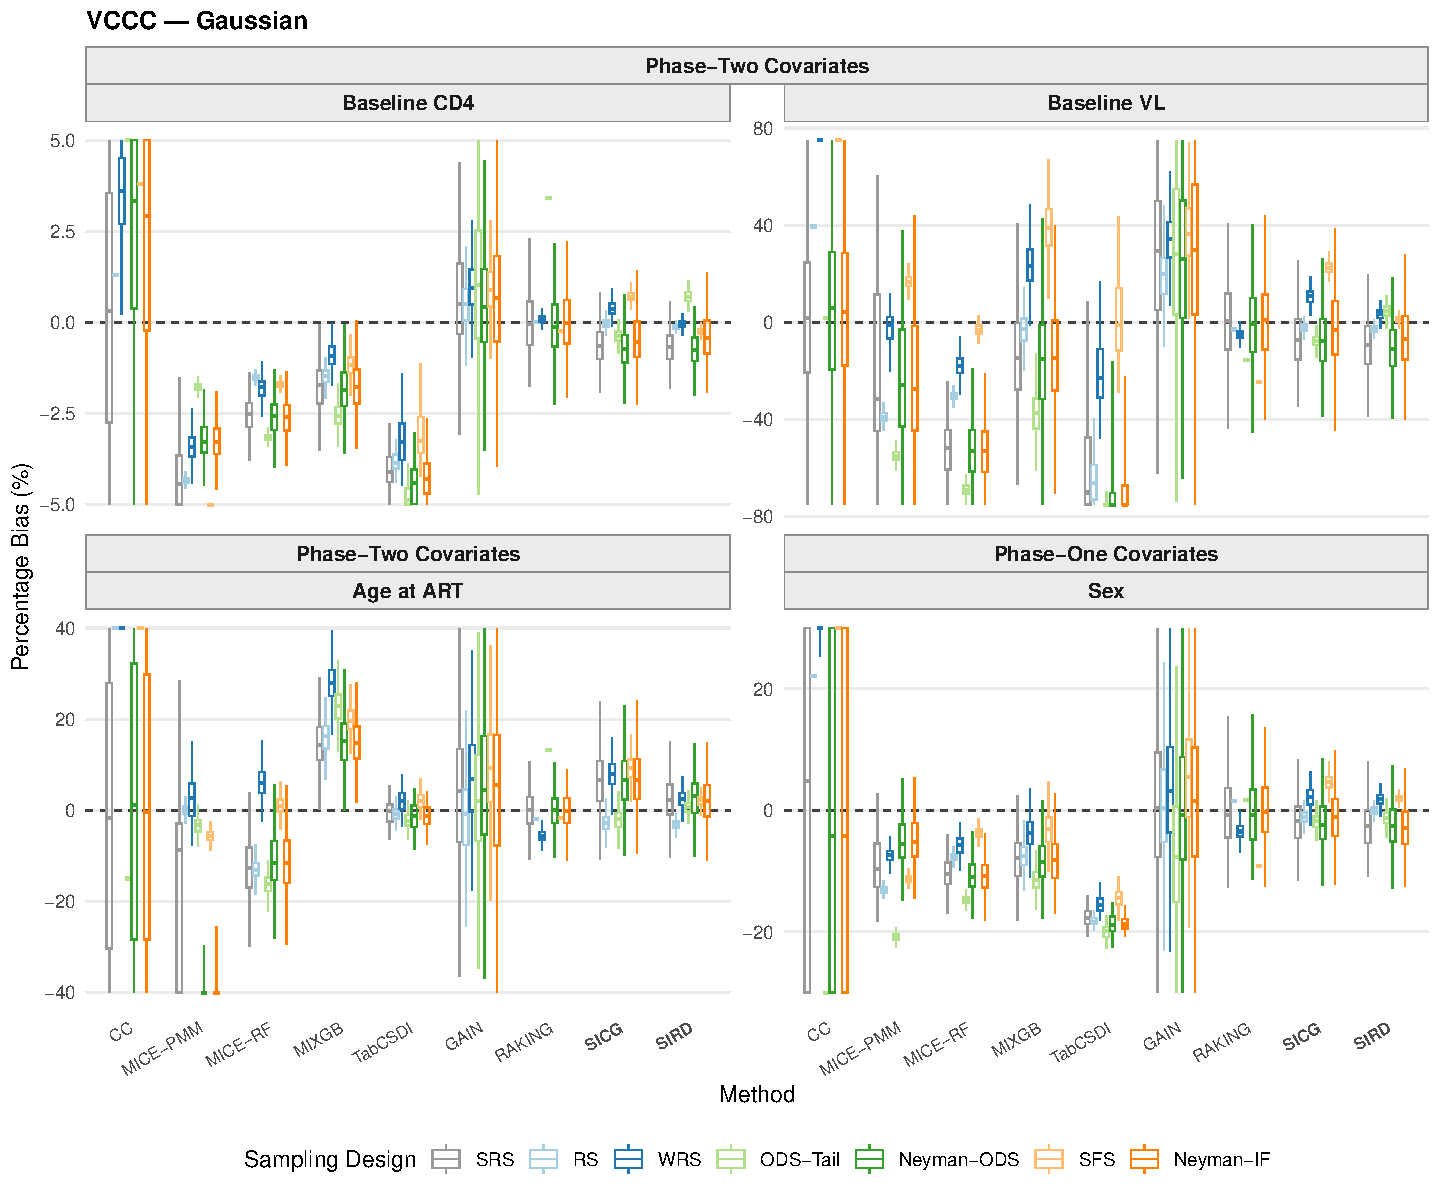
\includegraphics[width=\linewidth,height=0.86\textheight,keepaspectratio]{vccc_gaussian_pctbias.pdf}
\caption{Per-replicate percentage bias for the VCCC case study, Gaussian model, by method and sampling design; covariates grouped into Phase-Two and Phase-One.}
\label{fig:appc_vccc_gauss}
\end{figure}
\end{landscape}
\clearpage

\begin{landscape}
\begin{figure}[p]
\centering
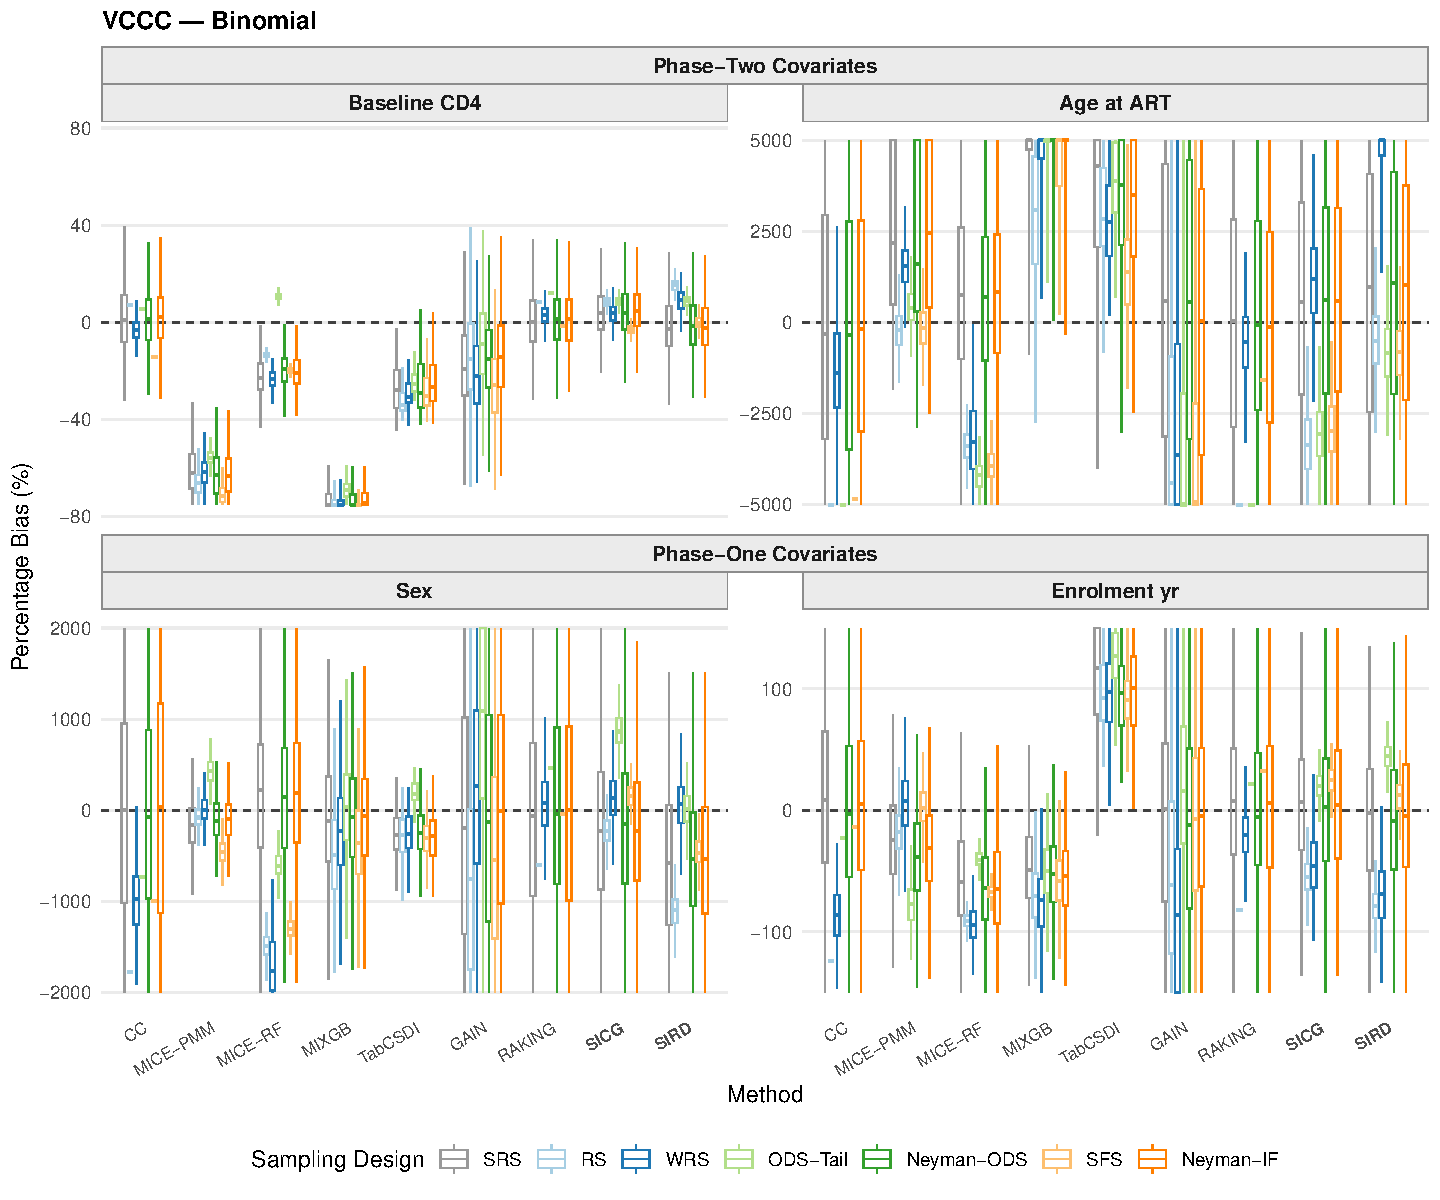
\includegraphics[width=\linewidth,height=0.86\textheight,keepaspectratio]{vccc_binomial_pctbias.pdf}
\caption{Per-replicate percentage bias for the VCCC case study, Binomial model.}
\label{fig:appc_vccc_binom}
\end{figure}
\end{landscape}
\clearpage

\begin{landscape}
\begin{figure}[p]
\centering
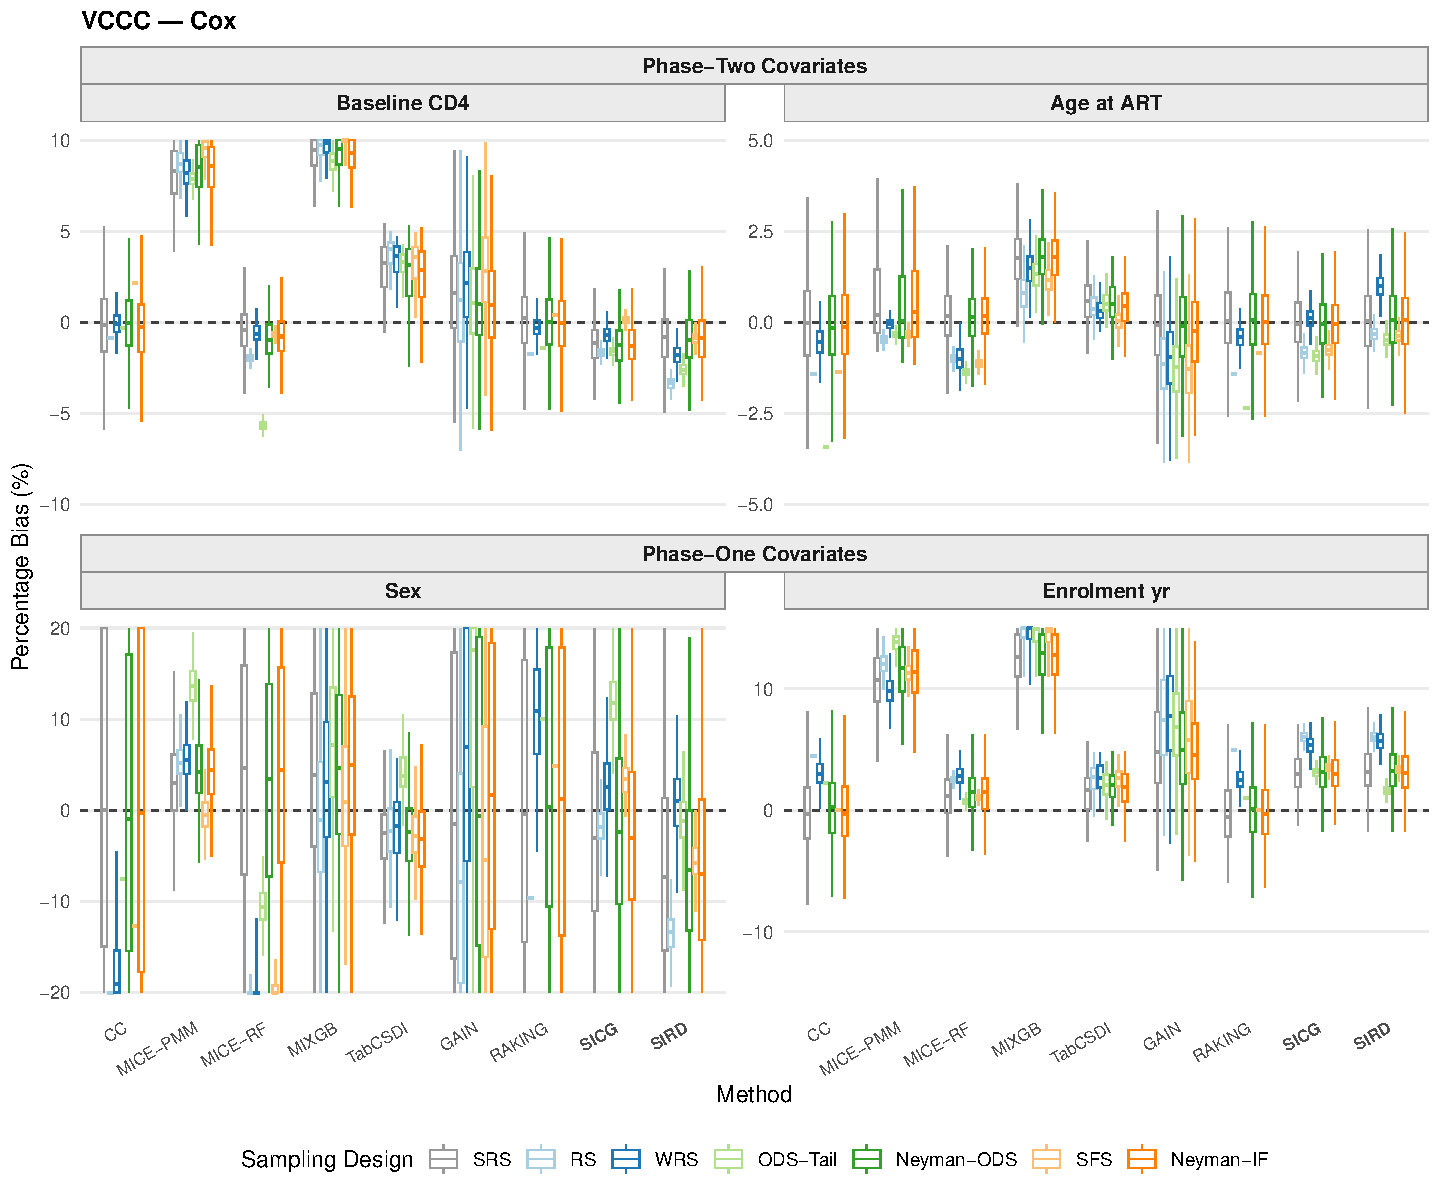
\includegraphics[width=\linewidth,height=0.86\textheight,keepaspectratio]{vccc_cox_pctbias.pdf}
\caption{Per-replicate percentage bias for the VCCC case study, Cox model.}
\label{fig:appc_vccc_cox}
\end{figure}
\end{landscape}
\clearpage

\FloatBarrier

\backmatter

\cleardoublepage
\bibliographystyle{plainnat}
\bibliography{bibliography}

\end{document}
